%%%%%%%%%%%%%%%% Springer %%%%%%%%%%%%%%%%%%%%%%%%%%%%%%%%%%


% RECOMMENDED %%%%%%%%%%%%%%%%%%%%%%%%%%%%%%%%%%%%%%%%%%%%%%%%%%%
\documentclass[graybox, envcountchap]{svmult}

% choose options for [] as required from the list
% in the Reference Guide
\usepackage[utf8]{inputenc}
\usepackage[charter]{mathdesign}       % selects basic font
\usepackage{helvet}         % selects Helvetica as sans-serif font
\usepackage{courier}        % selects Courier as typewriter font
\usepackage{type1cm}        % activate if the above 3 fonts are
                            % not available on your system
%
\usepackage[T1]{fontenc}

\usepackage{makeidx}         % allows index generation
\usepackage{graphicx}        % standard LaTeX graphics tool
                             % when including figure files
\usepackage{multicol}        % used for the two-column index
\usepackage[bottom]{footmisc}% places footnotes at page bottom
\usepackage[italian]{babel}
\usepackage[a4paper,top=2.5cm,bottom=2cm,left=2.5cm,right=2.5cm]{geometry}
\usepackage{float}
\usepackage{blindtext}
\usepackage[dvipsnames]{xcolor} %Usa i colori avanzati latex
\usepackage{titlesec}
\usepackage{wrapfig}

% Colori personalizzati
\definecolor{color_sigfied}{HTML}{007FFF} % Colore dei dettagli

\usepackage{pdfpages}


% Definizione nuovi comandi
\newcommand{\hsp}{\hspace{20pt}}

% FILIGRANA PER BOZZE
%\usepackage{draftwatermark}
%\SetWatermarkText{ 1\textsuperscript{o} Parziale}
%\SetWatermarkScale{0.7}

%Formattazione dei vari titoli
\titleformat{\chapter}[block]{\Huge\bfseries\sffamily}{Parte \thechapter\hsp\textcolor{color_sigfied}{}\hsp}{0pt}{\Huge\bfseries}
\titleformat{\section}[block]{\color{color_sigfied}\huge\bfseries\sffamily}{\thesection}{0.5em}{}
\titleformat{\subsection}[block]{\LARGE\bfseries\sffamily}{\thesubsection}{0.5em}{}
\titleformat{\subsubsection}[block]{\Large\sffamily}{\thesubsubsection}{0.5em}{}
\titleformat{\paragraph}[runin]{\normalfont\large\bfseries}{\theparagraph}{1em}{}
\titleformat{\subparagraph}[runin]{\normalfont\normalsize\bfseries}{\thesubparagraph}{1em}{}


\makeindex



%%%%%%%%%%%%%%%%%%%%%%%%%%%%%%%%%%%%%%%%%%%%%%%%%%%%%%%%%%%%%%%%%%%%%%%%%%%%%%%%%%%%%%%


\begin{document}

\includepdf[pages={1}]{igienecop.pdf}


\newpage\null\thispagestyle{empty}\newpage


\tableofcontents

\title*{Dispensa di Igiene, Sanità Pubblica e Politiche della Salute}
\titlerunning{Dispensa di Igiene, Sanità Pubblica e Politiche della Salute} 
\author{Gruppo Sigfied 2.0}
\maketitle
\newpage

\abstract{\textbf{Istruzioni per l'uso}
\begin{itemize}
\item Le dispense \textit{non} rappresentano un libro di testo perfetto ma un aiuto, crediamo molto valido, per orientarsi nello studio della materia;
\item Per la loro stessa natura le lezioni trascritte non sono scevre da errori sia di forma che di contenuto: per tanto vale il concetto aureo che per essere sicuri di un dato o di un concetto conviene cercare una rassicurazione su una fonte ufficiale;
\item I professori, spesso, ritengono questi materiali “ufficiosi” passibili di ogni denigrazione e li sconsigliano categoricamente agli studenti. È nostra opinione che, in realtà, le dispense costituiscano un valido ausilio per capire il filo conduttore da seguire per affrontare e studiare le tematiche mediche proposte dalla materia.
\end{itemize}
In bocca al lupo a tutti per gli esami!\\
\textbf{Gruppo Sigfied 2.0}}


\newpage

\section{LEZIONE INTRODUTTIVA AL CORSO INTEGRATO DI IGIENE E POLITICHE DELLA SALUTE}


Questa lezione è una lezione introduttiva in cui vengono spiegate oltre
alle modalità d'esame anche la gestione complessiva della didattica.

Questo corso è costituito da lezioni frontali a cui però, per la parte
di MEDICINA DI FAMIGLIA, si possono aggiungere delle visite ad alcune
strutture, per esempio alle case della salute come accaduto l'anno
scorso. ( le CASE DELLE SALUTE sono una forma aggregativa legata alla
medicina di famiglia e alla gestione soprattutto delle patologie cronico
degenerative).

\subsection{IL PROGRAMMA}


\textbf{1)EPIDEMIOLOGIA E PROFILASSI GENERALE DELLE MALATTIE INFETTIVE}(
questa parte si da per scontata che sia stata già fatta)
\begin{itemize}

\item misure di profilassi diretti e indiretti

\item vaccinoprofilassi, chemioprofilassi
\end{itemize}
\textbf{2)LA PREVENZIONE , SORVEGLIANZA E CONTROLLO DEI RISCHI SANITARI}
\begin{itemize}

\item concetti generali di prevenzione e sanità pubblica

\item metodologia epidemiologica

\item indicatori salutari e sistemi di sorveglianza

\item emergenze sanitarie e medicina delle catastrofi

\item rischi sanitari del viaggiatore internazionale

-educazione sanitaria e promozione della salute
\end{itemize}
\textbf{3)MALATTIE PREVEDIBILI CON VACCINI E ALTRE PATOLOGIE INFETTIVE}
\begin{itemize}

\item malattie vpd dell'infanzia. Il PNPV.

\item malattie vpd dell'adolescenza, dell'adulto, dell'anziano

\item calendari e strategie vaccinali

\item  malattie trasmissibili non vpo

\item  tossinfezione alimentare e HACCP

\item infezioni correlate all'assistenza
\end{itemize}
\textbf{4)ORGANIZZAZIONE SANITARIA ECONOMIA SANITARIA E MEDICINA DI
FAMIGLIA}
\\\\
\textbf{5)DETERMINANTI DI SALUTE E MALATTIA}
\begin{itemize}

\item epidemiologia malattie ad alto impatto socioeconomico

\item fattori di rischio modificabili e non modificabili

\item medicina preventiva e medicina predittiva, screening

\item incidenti, infortuni, e patologie comportamentali
\end{itemize}
\textbf{6)AMBIENTE E SALUTE}
\begin{itemize}

\item rischi ambientali e sviluppo sostenibile

\item inquinamenti atmosferici

\item ciclo idrico integrato

\item Urbanistica e salute e healthy buildings
\end{itemize}
\subsection{INTRODUZIONE}


Ricordiamo che per fare sanità pubblica non servono solo medici ma a
seconda degli approcci, servono inoltre diverse categorie, molto spesso
``decisori'' ovvero dal ministro della salute in giù, cioè chi prende
decisioni di politica sanitaria.

In tutto il corso di igiene ci sono 2 punti fermi:

\begin{enumerate}
\def\labelenumi{\arabic{enumi})}
\item
  Le priorità di sanità pubblica
\item
  Cosa si può fare in termini di prevenzione
\end{enumerate}

  Non a caso è stata mostrata una diapositiva che riguarda la campagna
  pubblicitaria per ridurre il sodio , che ha un suo ruolo come fattore
  di rischio delle malattie cerebrovascolari. Questo è un tema
  importante e prioritario in sanità pubblica poiché le morti per
  malattie cardiovascolari sono la prima causa di morte in Italia. Se
  noi agiamo sul fattore dieta possiamo fare molto in termini di
  riduzione di incidenza di mortalità da malattie
  cerebrovascolari.Perciò in tutto il corso cercheremo di identificare
  le priorità e di identificare dove la prevenzione può arrivare.

  I medici non hanno più quella piena e completa autonomia e devono fare
  i conti con patti, piani e nuove normative. L' Italia ha un servizio
  sanitario nazionale, che affronteremo come argomento a Novembre, lo
  sentiamo sempre con lo slogan ``la libertà di cura'' cioè ciascun
  cittadino per alcune prestazioni ( le più importanti) ha le cure
  gratuite o pagando un ticket di entità bassa rispetto alla prestazione
  che riceve. Questa cartina ci dice che siccome c'è libertà di
  circolazione, ovviamente quando si tratta di un emergenza il paziente
  tenderà ad andare nell'ospedale piu vicino, ma quando l'intervento
  chirurgico è programmato, quando il ricovero per far diagnosi è
  programmabile e dilazionabile , li ci sono i movimenti per l'italia

  Le regioni segnate in rosso sono le regioni che hanno una quantità di
  pazienti che migrano in altre regioni superiori al 5\% dei ricoveri.
  La Liguria ad esempio essendo circoscritta da diverse regioni verdi (
  sono verdi le regioni che accettano molto) tende ad avere un flusso
  alto verso le altre regioni. Al centro- sud invece vediamo un
  agglomerato di regioni rosse, qui evidentemente c'è un problema grosso
  di flusso di pazienti verso le regioni verdi ad esempio Emilia
  Romagna, Veneto, Lombardia significa che le strutture non sono buone o
  ritenute tali o c'è qualcosa che non va nell'organizzazione sanitaria
  di quelle regioni. ( questo argomento verrà comunque trattato più
  avanti). Il legislatore sanitario in questo caso deve fare delle
  riflessioni profonde riguardo alle ``migrazioni regionali'' perché non
  è che se la regione Sicilia perde il20\% dei ricoveri vada a
  risparmiare, anzi! Perché il meccanismo è tale per cui il ricovero del
  siciliano è pagato dal servizio sanitario della Sicilia anche se va a
  farsi curare fuori, con un contributo economico da parte della ragione
  Sicilia alla struttura alla quale il paziente si è rivolto secondo
  precisi tariffari. Perciò laddove c'è ``la fuga'' c'è un grave
  problema di dissesto economico in queste regioni, poiché i medici
  assunti ,quelli sono e quelli rimangono, avremo posti letto vuoti ,
  costi uguali e spese maggiori perché devono anche pagare il DRG ,
  ovvero la tariffa che viene pagata per la prestazione di ricovero alle
  regioni dove queste persone si sono rivolte per curarsi. Questo è un
  flash per far capire come la sanità in realtà sia più complicata del
  previsto.

  La tabella di sinistra ( grafico a barre: in questo caso la lunghezza
  della barra corrisponde alla percentuale del PIL che viene speso nella
  sanità nei paesi Europei). Possiamo notare che l' Italia è a metà
  classifica, ma considerando che dentro a quel valore di 9.2 prcento
  del PIL (che è una cifra spaventosa , siamo attorno a 150 miliardi di
  cui 120 miliardi spesi dal pubblico e i 30 restanti dal circuito delle
  prestazioni private. Per capire quanti siano questi 150 miliardi : lo
  stato spende in media 1800 euro per ogni cittadino all'anno!). Anche
  questo è un flash , sarà un argomento trattato più avanti.

  Parlando di \textbf{METODOLOGIA EPIDEMIOLOGICA} , che è una parte di
  corso ,noi illustreremo:

\begin{itemize}
\item
  Che cos'è l'epidemiologia
\item
  Quali sono gli strumenti di lavoro
\item
  Fonti dei dati, misure , lettura e interpretazione dei dati
\item
  C'è un'aggiunta che riguarda l'epidemiologia clinica: cioè
  l'applicazione dei metodi epidemiologici a quegli studi che
  sostanzialmente validano le terapie, anche gli approcci preventivi e
  vanno a far maturare le esigenze e le evidenze scientifiche.
\end{itemize}

  Vedremo inoltre la parte delle MALATTIE INFETTIVE, e qui emerge la
  gestione dell'evento infettivo quando ci sono situazioni di epidemie
  di scala mondiale, ma leggendo i giornali oggi si parla di un caso di
  epidemia di Legionellosi a parma , che è un epidemia su piccola scala
  ma che ha acceso i riflettori su una provincia , su una patologia e
  anche qui servono interventi e prese di posizione sul fronte della
  gestione.
\\\\
  Ci dedicheremo alla questione delle vaccinazioni e cercheremo almeno
  in una lezione di non trascurare un fenomeno esistente, ovvero ci sono
  vaccini sempre più efficaci e sempre meno gente che si vaccina ( un
  po' come la questione dello screening) e ciò è un po' la frustrazione
  di chi si occupa di prevenzione, che però qualcosa può fare ovvero
  cercare di capire ciò accada.

  Vedremo poi i determinanti di malattia qui c è un grafico che mostra
  in che modo i fattori esterni possono influenzare l'incidenza e lo
  sviluppo di malattia.
\\\\
  Ha peso del 5\% la genetica, ci sono il 5\% di malattie dove noi
  possiamo fare poco in realtà, possiamo al più fare diagnosi precoce.

  Su tutto il resto ci sono fattori esterni su cui noi possiamo lavorare
  molto bene a volte. L' ambiente è considerato non solo come ambiente
  fisico ma anche sociale,in quanto i luoghi di vita e le condizioni di
  vita in generale possono avere influenza sull'andamento di alcune
  malattie. Poi ci sono gli `` health behaviors'' che sonoi
  comportamenti individuali , e i ``medical care'' che sarebbe il
  servizio sanitario in grado di far fronte ai bisogni della
  popolazione. Mettendo tutto insieme facciamo il 100\%. Possiamo
  lavorare su quasi tutti questi ambiti cercando di ridurre l'impatto
  delle malattie.
\\\\
  Il tema DELL'AMBIENTE è esemplificato da 3 fotografie che non sono
  casuali ( manca diapo) una fotografia classica che parla
  dell'inquinamento tradizionale dell'aria ( tema rilevante in ITALIA e
  soprattutto in Pianura Padana). Settimana scorsa è uscito un rapporto
  che classificava la salute degli italiani , mettendo alcuni aspetti
  positivi, uno di questi al servizio sanitario nazionale che comunque è
  universalistica e fa fronte alle principali esigenze sanitarie e
  mettendo in evidenza inoltre le debolezze nazionali principali tra cui
  ricordiamo l'inquinamento atmosferico riferito soprattutto al nord
  Italia poiché è più inquinato per motivi climatici e geografici .Anche
  questo tema verrà esplicato più avanti.
\\\\
  A questo punto il prof ha introdotto due concetti base:

\paragraph{lo stato di salute}
  

  Definizione : completo stato di benessere fisico, sociale , mentale e
  non soltanto assenza di malattia.

\paragraph{La sanità pubblica}
  

  Definizione: è l'organizzazione che mobilita risorse scientifiche,
  tecniche e professionali ed economiche per far fronte ai problemi
  sanitari delle popolazioni cercando di garantire loro il miglior stato
  di salute.

  Da ciò capiamo che la strategia della sanità pubblica non è uguale
  dappertutto, cioè se faccio sanità pubblica in Uganda non ho gli
  stessi problemi dell' Italia per cui ne consegue che l'approccio sarà
  completamente diverso. In Uganda l'epidemiologia ci dice che ci sono
  malattie infettive ad incidenza altissima, pochi anziani e tanti
  bambini, quindi dovrò commisurare tutti gli interventi a quella
  situazione demografica e sanitaria.

  Cerchiamo di vedere la principale differenza tra la sanità pubblica e
  l'attività medica clinica:

  la medicina clinica salva una vita per volta , la sanità pubblica
  dovrebbe arrivare a salvare milioni di vite (soprattutto tramite la
  PREVENZIONE . La prevenzione lavora a lungo termine si basa su
  evidenze scientifiche tende ma l operazione è in corso a lavorare sul
  consenso e sulla responsabilizzazione individuale senza quello la
  prevenzione fallisce. Ci stiamo ad esempio adoperando per uno studio
  che riguarda il vaccino per lo zoster, e sappiamo che molti non sono a
  conoscenza dell'esistenza del vaccino e ciò sarebbe perdonabile da
  parte di un cittadino anziano, la cosa grave è che nemmeno i medici
  sanno molte volte dell'esistenza del vaccino. Per cui bisogna
  informare e responsabilizzare.

  Esistono diversi tipi di prevenzione:
  \begin{itemize}

\item
  La primaria che cerca di rimuovere i rischi e proteggere gli esposti
  ai fattori di rischio ( es. tramite i vaccini)
\item
  La secondaria che fa diagnosi precoce e identifica situazioni a
  rischio
\item
  Prevenzione attiva che fa interventi sulla persona ( ex. Vaccini e
  screening)
\item
  Prevenzione collettiva
  \end{itemize}
\subsection{COME SI SVOLGERà L'ESAME DI IGIENE E SANITA'  PUBBLICA}

Innanzitutto è un esame di 12 crediti. 
Come si svolge l’esame: per tutto l’anno viene garantita la possibilità di svolgere un quiz di 36 domande a scelta multipla su tutto il programma più orale finale. Invece per la prima fase dell’anno fino a febbraio , si possono svolgere i 3 compiti a quiz , suddividendo così la materia , più sempre un orale. Il voto finale dipenderà molto dalla media dei 3 scritti, si arriverà all’orale con un certo range di voto ( ad esempio tra il 26 e il 28) e l orale quindi non modificherà più di tanto l’esito finale.
La prima prova verterà su 2 argomenti( saranno 12 domande e il primo appello sarà tra la metà e la fine di novembre, la seconda possibilità di darlo sarà a Dicembre e altre fino a fine Febbraio):
\begin{itemize}

\item epidemiologia e prevenzione delle malattie infettive
\item metodologia epidemiologica
\end{itemize}
La seconda parte comprende argomenti trattati da inizio Novembre e termina a Natale( l’appello sarà dal 15 Dicembre in poi) :
\begin{itemize}

\item economia sanitaria e organizzazione sanitaria
\item le altri parti le stiamo valutando
\end{itemize}
Tutto ciò che manca verrà messo nel terzo e ultimo compito a Gennaio/Febbraio

Superando i diversi compitini che avranno un giudizio ( sufficiente, discreto, buono, ottimo) si avrà un giudizio finale che corrisponde a un range di voto e si accede con questo poi all’orale.

Ci sono alcune parti in cui il materiale delle lezioni è sufficiente come per esempio Bioetica, o la parte di medicina generale , per altre invece va fatta  integrazione soprattutto per questi argomenti:
\begin{itemize}

\item Organizzazione sanitaria
\item Metodologia epidemiologica
\item Profilassi malattie infettive
\item Alimenti e ambiente
\end{itemize}

\section{Fonti dei dati, indicatori sanitari, sorveglianza}

\subsection{Cronaca}


La Gazzetta di Parma del 05/10/2016 riporta 3 notizie legate alla Sanità
Pubblica:

\begin{enumerate}
\def\labelenumi{\arabic{enumi}.}
\item
  La seconda vittima di Legionella e il 31esimo caso, siamo di fronte ad
  un'epidemia
\item
  Capitolo ambiente, gestione dei rifiuti
\item
  La modifica costituzionale include anche cambiamenti per quanto
  riguarda la materia sanitaria (verrà trattata nelle lezioni di
  organizzazione sanitaria); vengono riportate allo stato alcune
  competenze legislative che erano state date nel 2001 alle regioni,
  quindi, se il referendum verrà approvato, dal punto di vista della
  struttura del sistema sanitario ci saranno più decisioni al centro e
  meno nelle regioni
\end{enumerate}

L'epidemia in corso riguarda la Legionella, un batterio ambientale, non
c'è trasmissione interumana dimostrata, c'è contaminazione ambientale in
vario modo: soprattutto immissione di aria o di aerosol nell'ambiente.
Gli ultimi focolai epidemici hanno riguardato condutture idriche o
impianti di distribuzione dell'aria.

Com'è stata scoperta la legionellosi 40 anni fa? È stata scoperta perchè
ci fu una riunione a Philadelphia di veterani del Vietnam che si
ritrovano annualmente cercando alberghi non utilizzati, fuori dalle
stagioni turistiche per spendere poco. Questi alberghi venivano riaperti
per queste convention e la Legionella, se viene lasciata nei filtri
d'aria, non ben mantenuti, presenti negli impianti di climatizzazione,
si moltiplica e alla riaccensione degli impianti viene immessa in
quantità importante nell'aria. Ciò ha portato ad un'epidemia. Inoltre i
veterani avevano una certa età, e quindi ci fu il primo caso epidemico
di Legionella che da quel momento in poi fu battezzata ``la malattia dei
legionari''.

La legionella è un batterio ambientale che, se presente in basse
concentrazioni non porta grandi rischi, a meno che ci sia una
suscettibilità dell'ospite (secondo elemento che nell'attuale epidemia è
fondamentale). Quindi, c'è una fonte d'immissione, probabilmente nel
caso di Parma sono le condutture idriche. Nelle condutture idriche poco
utilizzate, con incrostazioni, la Legionella c'è, si moltiplica in un
range di temperatura che va dai 20 ai 40C; si tratta di condutture in
stagione estiva o condutture dove passa l'acqua calda e quindi le
Legionelle vengono immesse nell'aria alla riapertura delle condutture
come aerosol e vengono respirate. A volte possono esserci microepidemie
nelle strutture ospedaliere. La legionella è termolabile, per cui con
l'acqua a 60C c'è l'inattivazione, come per l'acqua a temperature
minori.

Una precauzione individuale è quella di lasciar un po' scorrere l'acqua
prima di lavarsi la faccia, perchè altrimenti viene respirato l'aerosol
del primo getto; ciò riguarda soprattutto impianti usati poco, perchè se
sono impianti usati molto il problema non si pone. Se lo respira un
soggetto giovane immunocompetente non gli succede nulla, ha una forma
asintomatica; ma se lo respira un immunodepresso o un anziano può dare
molti problemi. A Parma non è ancora stata identificata esattamente la
fonte di partenza.

Quando ci sono i morti la psicosi epidemica ha sempre un forte impatto.

\subsection{Fonti dei dati}


Gli argomenti del primo parziale, sono 2: Metodologia epidemiologica,
Profilassi delle malattie infettive. Verranno trattatati fino all'ultimo
Venerdì di Ottobre, in totale dovrebbero essere 11 lezioni.

\subsubsection{Epidemiologia}


\begin{itemize}
\item
  Deriva dal greco ``studio sul popolo''
\item
  Scienza che studia le malattie e i fenomeni ad essere correlati a
  livello di popolazione
\item
  Include studi sulla frequenza delle malattie, sui fattori di rischio,
  sui servizi sanitari
\end{itemize}

L'epidemiologia nasce come disciplina che studia le epidemie delle
malattie infettive: Colera (Londra, 1870). Nasce per studiare le
malattie infettive, ma in un secondo tempo con gli stessi metodi si sono
studiate le malattie non infettive, i fattori di rischio e i
bisogni/servizi sanitari.

Siamo abituati a considerare l'epidemiologia uno strumento e non una
disciplina: è uno strumento che si applica spesso alla sanità pubblica e
alla medicina clinica.

Queste lezioni hanno lo scopo di farci comprendere le principali
tecniche epidemiologiche che possono essere usate in sanità pubblica, ma
anche nelle varie discipline/specialità con qualche aggiustamento e
particolarità.

Esempio 1. L'epidemiologia psichiatrica ha come punto debole del
meccanismo di valutazione il fatto che le diagnosi sono variopinte e non
sempre riconducibili a delle situazioni oggettive.

Esempio 2. L'epidemiologia dei tumori ha a che fare con dei dati molto
più oggettivi, però chiede di occuparsi dei fattori di rischio (non
sempre facilmente analizzabili).

C'è una parte dell'epidemiologia (clinica) applicata alle
sperimentazioni dei nuovi farmaci/trattamenti ed è quello strumento che,
insieme alla statistica, consente di poter fare le sperimentazioni e di
poter dimostrare, dove possibile, che nuovi trattamenti sono migliori di
quelli descritti.

Quindi abbiamo a che fare con uno strumento di lavoro che, come tale,
deve basarsi su dati.

L'epidemiologia analizza dati. In 2 modi l'epidemiologia si occupa di
dati:

\begin{enumerate}
\def\labelenumi{\arabic{enumi}.}
\item
  \textbf{approccio DESCRITTIVO}: descrive i fenomeni sanitari.
\end{enumerate}

\begin{quote}
Prende dati esistenti, già presenti e raccolti attraverso le fonti, li
riordina/analizza/stratifica e produce le statistiche sanitarie. Magari
con qualche correlazione tra l'andamento di un fenomeno e condizioni
esterne, ambientali, sociali, economiche; ma tendenzialmente descrive il
fenomeno. Difficilmente con la descrizione dei fenomeni si riesce ad
arrivare all'identificazione delle cause che, invece, attiene alla parte
dell'epidemiologia analitica.
\end{quote}

\begin{enumerate}
\def\labelenumi{\arabic{enumi}.}
\item
  \textbf{approccio ANALITICO}: indagare le cause / i determinanti.
\end{enumerate}

\begin{quote}
Accanto ai dati esistenti si cercano dati oggettivi per poter associare
la malattia ai fattori di rischio. Es. per scoprire la causa della
Legionella bisogna vedere caso per caso, vedere dove vivono, che
abitudini hanno le persone, se sono state o meno esposte a certi fattori
di rischio che potrebbero esser quelli ad aver causato la sua
diffusione.
\end{quote}

Quindi, l'epidemiologia descrittiva elenca i casi, l'analitica va a
cercare le cause e non sempre ci riesce.

Per soddisfare il primo obiettivo, i dati spesso ci sono, anche se non
sempre sono attendibili al 100\%. A volte sono disponibili ed
utilizzabili immediatamente, a volte sono parzialmente disponibili
(ossia sono raccolti ma devono essere elaborati), altre volte non ci
sono (bisognerà fare indagini ad hoc per cercarli).

\paragraph{Fonte di dati epidemiologici}


\begin{itemize}
\item
  Dati disponibili
\item
  Dati parzialmente disponibili
\item
  Dati non disponibili
\item
  Finalità sanitaria
\item
  Finalità amministrativa
\item
  Finalità di ricerca
\item
  Dati aggregati
\item
  Dati individuali
\end{itemize}

Esempio di \textbf{dati sanitari disponibili} (aprendo il computer e
cercandoli): schede di dimissione ospedaliera e report sulle cause di
ricoveri in Italia. A livello centrale si raccolgono i dati sui ricoveri
che hanno un duplice significato: finalità sanitaria, ma soprattutto una
finalità amministrativa.

Le schede di dimissione ospedaliera:

\begin{enumerate}
\def\labelenumi{\alph{enumi})}
\item
  sono fatte per tutti i pazienti dimessi
\item
  tendono a riportare le diagnosi di dimissione in maniera abbastanza
  precisa, perchè da quello dipende il rimborso alla struttura
  ospedaliera per la prestazione erogata
\item
  devono essere attendibili, perchè soggette a controlli
\end{enumerate}

Esempio di \textbf{dati sanitari parzialmente disponibili}: cartelle
cliniche (i dati ci sono ma non sono raccolti e rielaborati). Se voglio
fare una ricerca per una determinata malattia: prendo, con tutti i
permessi e i nulla osta dei comitati etici, le cartelle cliniche,
raccolgo e ricopio tutti i dati che a noi interessano.

Esempio di \textbf{dati sanitari non disponibili} (non c'è nessuna fonte
che li raccoglie). È il gruppo più numeroso. Se volessi sapere quanti
sono i fumatori in Italia i dati non li troverei. Non c'è un elenco
nazione dei fumatori, come non c'è l'obbligo di dichiarare le proprie
generalità all'acquisto di tabacchi. Non ho i dati, ma posso stimarli in
2 modi: prendendo il dato del Monopolio di Stato che ci dice quanti
pacchetti di sigarette sono venduti, questo è un dato che può monitorare
il trend degli anni oppure facendo un'indagine a campione (telefonate a
casa o questionari).

Quindi, quando studio un problema, devo sempre chiedermi se i dati ci
sono o meno.

Ci sono situazioni in cui posso cercare di prendere i dati ma questi non
sono attendibili: più delicato è il tema, più difficile è la raccolta
del dato, soprattutto sulle abitudini individuali.

Es. Se volessi analizzare quante sono le lesioni da morsicatura di cane.
Negli USA muoiono ogni anno 20 persone morsicate da un cane, in Italia
ne muoiono 3-4. Nelle schede dei pronti soccorsi troviamo quanti
pazienti entrano con la diagnosi di morsicatura di animale e i dati sul
ricovero se la lesione è grave. Non ho modo di trovare dati che
riguardano le medicazioni ambulatoriali o le automedicazioni, devo fare
delle stime, ma a volte l'indagine campionaria può non essere
attendibile spesso perché i soggetti coinvolti non ricordano. Un'altra
grande difficoltà si ha nelle indagini nutrizionali, se chiedo ad un
campione di persone di raccontarmi ciò che ha mangiato nell'ultimo anno
e qual è il pasto medio, è possibile che non si ricordino e quindi non
forniscono un dato attendibile.

Il dato deve essere sempre pesato in relazione alla sua attendibilità.

Ho dati di attendibilità piena, come la scheda di morte che è un dato
oggettivo, sempre presente; sulle cause di morte i dati sono meno
attendibili, perchè ci può essere qualche notifica non precisa.

Tra i dati disponibili: schede di morte, schede di nascita, notifica
delle malattie infettive, schede di dimissione ospedaliera, cartelle
cliniche. Oltre a questa fonte di dati prettamente sanitari, abbiamo
dati più demografici/economici come il censimento che raccoglie dati
demografici, economici, sugli ambienti di vita, sulla mobilità.


\begin{figure}[!ht]
\centering
	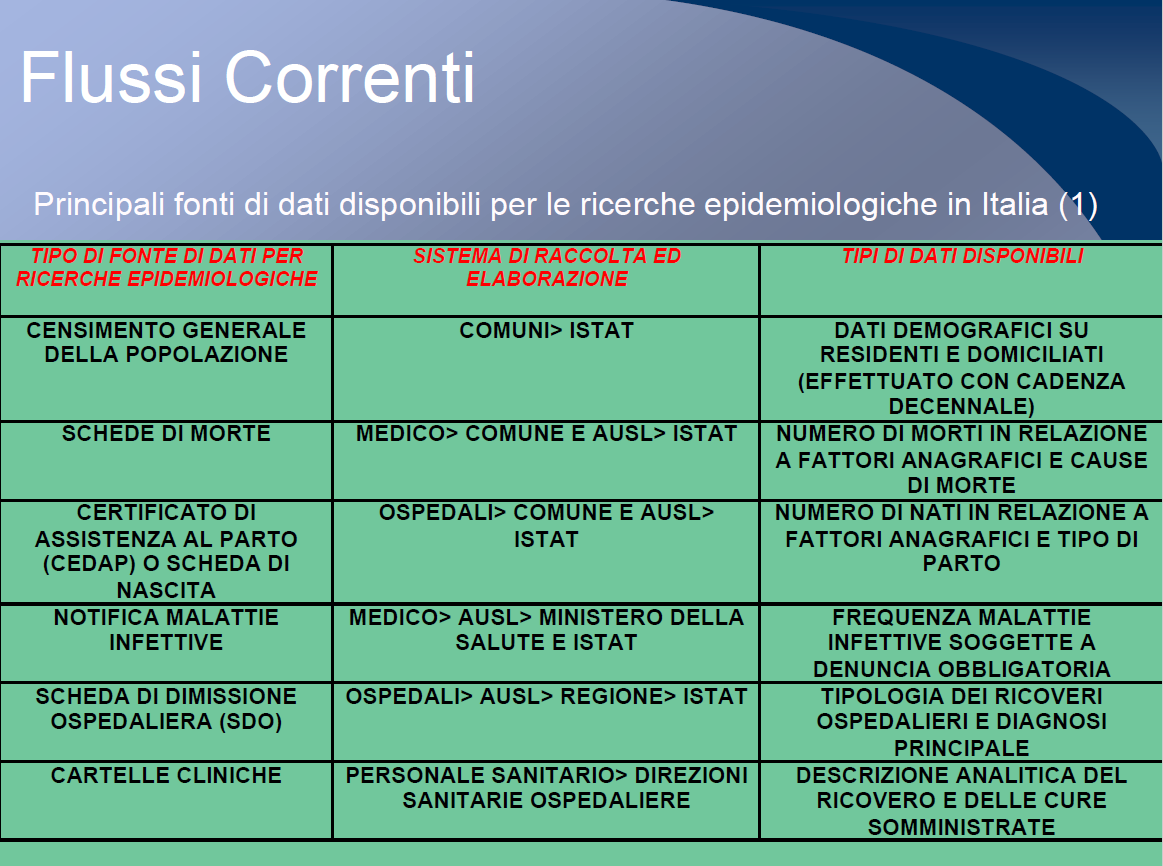
\includegraphics[width=0.9\textwidth]{02/image1.png}
\end{figure}



\paragraph{Notifica delle malattie infettive}

La notifica delle malattie infettive merita una segnalazione. Ogni tanto
c'è qualche caso di Legionella, oggi a Parma c'è un episodio epidemico;
ma i casi di Legionellosi comunque ci sono. Se sono lievi la probabilità
che questi casi vengano notificati non è altissima, cioè il medico
potrebbe, se i sintomi sono generici e aspecifici, non chiedere indagini
diagnostiche e quindi quel caso non è notificato oppure il medico
potrebbe, anche in presenza di accertamento diagnostico, non notificare
perchè il paziente viene visitato in ambulatorio dove i tassi di
notifica sono meno stringenti rispetto alla struttura ospedaliera.
Quindi noi siamo certi che tutte le Legionellosi che arrivano in
ospedale vengano notificate, ma non ne siamo affatto certi per le
Legionellosi che arrivano in ambulatorio.

La notifica delle malattie infettive risente della sottonotifica, questa
è tanto maggiore quanto di minor gravità è la malattia. Se leggo sulle
statistiche che ci sono 1000 casi di malaria all' anno, ritengo che
questo dato sia molto attendibile; perchè la malaria è una malattia che
quando viene vista viene notificata.

Quando trovo 1000 casi di morbillo, non sono convinto che questi siano
in realtà tutti casi di morbillo; perchè abbiamo a che fare con una
malattia che nella maggior parte dei casi è di lieve impatto e non
sempre viene notificata: vengono notificati circa 2 casi su 10 di
morbillo, quindi abbiamo il 20-30\% di tasso di notifica.

Quando ci sono le epidemie, i medici diventano scrupolosissimi, quindi
dei 31 casi di Legionellosi a Parma siamo certi, perchè oggi qualunque
caso di sospetta Legionellosi richiede l'accertamento diagnostico.
Quindi l'episodio epidemico tende a rende il medico più scrupoloso nella
diagnosi e nella notifica del caso. Dunque, anche la stessa fonte, in
momenti diversi, può essere più o meno attendibile.


\begin{figure}[!ht]
\centering
	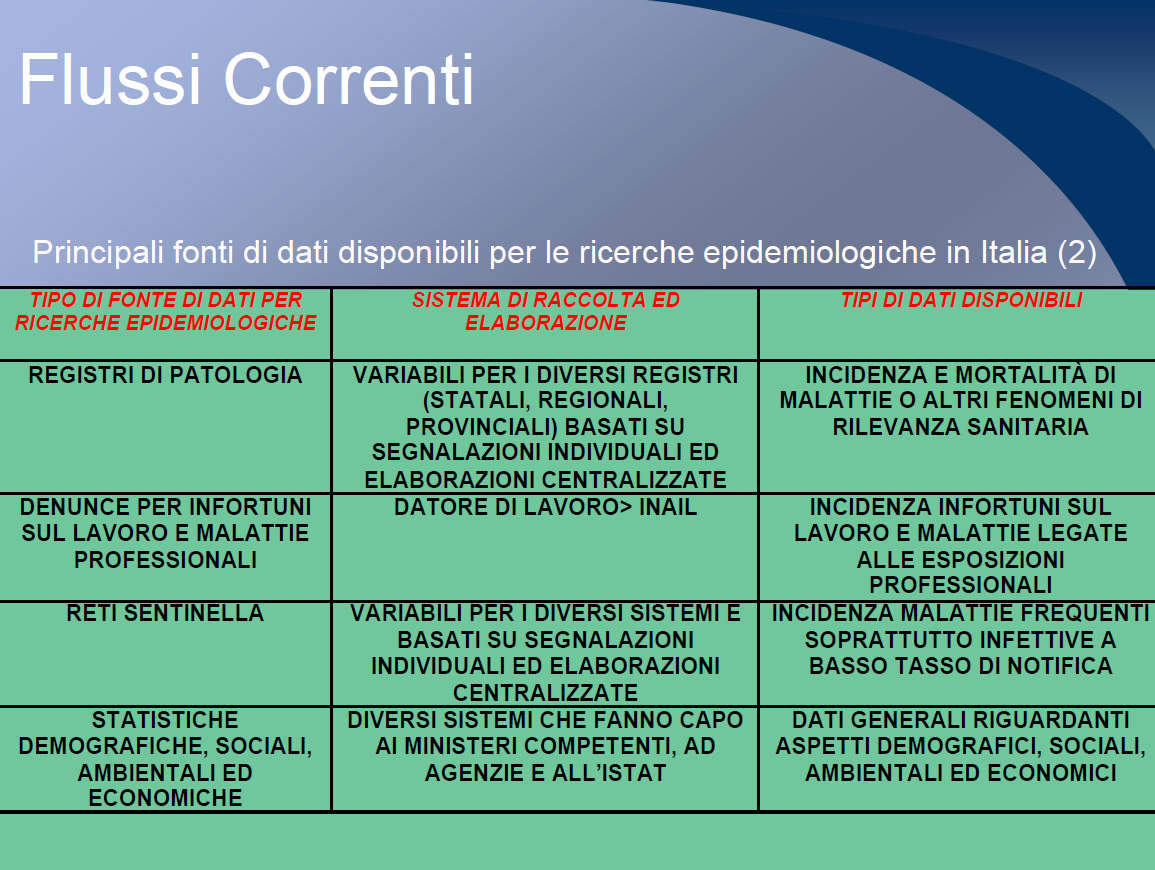
\includegraphics[width=0.9\textwidth]{02/image2.png}
\end{figure}


\paragraph{Registri di patologia}


Es. registro dei tumori (c'è a Parma e in altre 15 province italiane).

Al contrario delle malattie infettive, noi non abbiamo l'obbligo di
notifica dei tumori, però il paziente col tumore, durante la sua
malattia (solitamente nelle prime fasi) va in ospedale, quasi tutti i
tumori maligni accedono ad una struttura ospedaliera, quindi avranno la
loro SDO e questa avrà una diagnosi che riporterà quel tumore, se
confermato da accertamenti diagnostici.

Se vado a leggere quanti ricoveri per tumore al polmone ho in un anno
tra i residenti nella provincia di Parma e scopro che sono 2500 ricoveri
con diagnosi di tumore al polmone, questo dato mi serve ai fini di
valutare il numero di tumori o i nuovi casi di tumore? No. Da
epidemiologo mi serve sapere quanti sono i nuovi casi, quanti sono i
casi presenti e sapere come negli anni va la malattia. Quindi questo
dato non mi basta, perchè i 2500 potrebbero essere tutte persone che
entrano una volta, ma anche meno persone che vengono ricoverate più
volte, alcuni di questi potrebbero già avere il tumore e rientrare in
ospedale per una complicazione o una cura, altri sono nuovi casi. In
realtà i dati ci sono ma occorre riordinarli per poter calcolare
l'incidenza della malattia.

Il registro tumori raccoglie tutti i dati diagnostici incrociandoli con
i dati anagrafici e compone un quadro per tutti i tumori maligni di
numero di nuovi casi, incrociandoli con le schede di morte di questi
pazienti, si riesce anche ad avere il dato di mortalità e anche di
letalità dei tumori (i dati di sopravvivenza dalla prima diagnosi). Il
registro tumori dà dei risultati attendibili. Il presupposto
fondamentale è che ci sia l'accesso al sistema ospedaliero di tutti i
tumori, è quasi vero, perchè perdiamo qualche paziente che si cura in
strutture private o all'estero (questi casi non vengono visti dalle
statistiche). Le SDO sono compilate dalle strutture pubbliche e dalle
strutture private accreditate di tutta Italia, quindi è possibile con
agilità ricostruire i dati dei cittadini di Parma che vanno a farsi
curare in tutta Italia, perchè la SDO arriva all'ASL per il pagamento
della prestazione. Però in Italia l'accesso delle strutture private
pure, è marginale per malattie di questo tipo (tumori).

Si tratta di dati che non potrei avere in nessuna delle altre fonti,
nella scheda di morte c'è la causa di morte, ma non tutti i tumori sono
ad alta letalità e qualcuno guarisce anche; quindi dal punto di vista
epidemiologico non sono soddisfatto dal dato di mortalità, lo potrei
essere per i tumori ad alta letalità, ma fortunatamente oggi molti
tumori non hanno una letalità altissima. Quindi per avere i dati
d'incidenza devo avere il registro dei tumori.

\paragraph{Reti sentinella}


Ci sono situazioni dove la malattia non è cosi grave da determinare il
ricovero ospedaliero, dove le notifiche non sono fatte bene, dove non si
muore o si muore molto poco. Un caso emblematico è l'influenza
(\textbf{sindrome} \textbf{influenzale}): si muore raramente, non si va
in ospedale se non per fatti gravi. In questi casi esiste una rete
sentinella in cui un campione ormai consolidato di medici di famiglia,
sparsi su tutto il territorio nazionale, fanno notifica attraverso un
sistema consolidato all'istituto superiore di sanità, secondo le linee
guida internazionali, ogni qual volta riscontrano sintomi riconducibili
all'influenza, secondo un protocollo che viene stabilito e con un certo
margine di errore/imprecisione che, però, è calcolato e può esser tenuto
in conto.

\begin{figure}[!ht]
\centering
	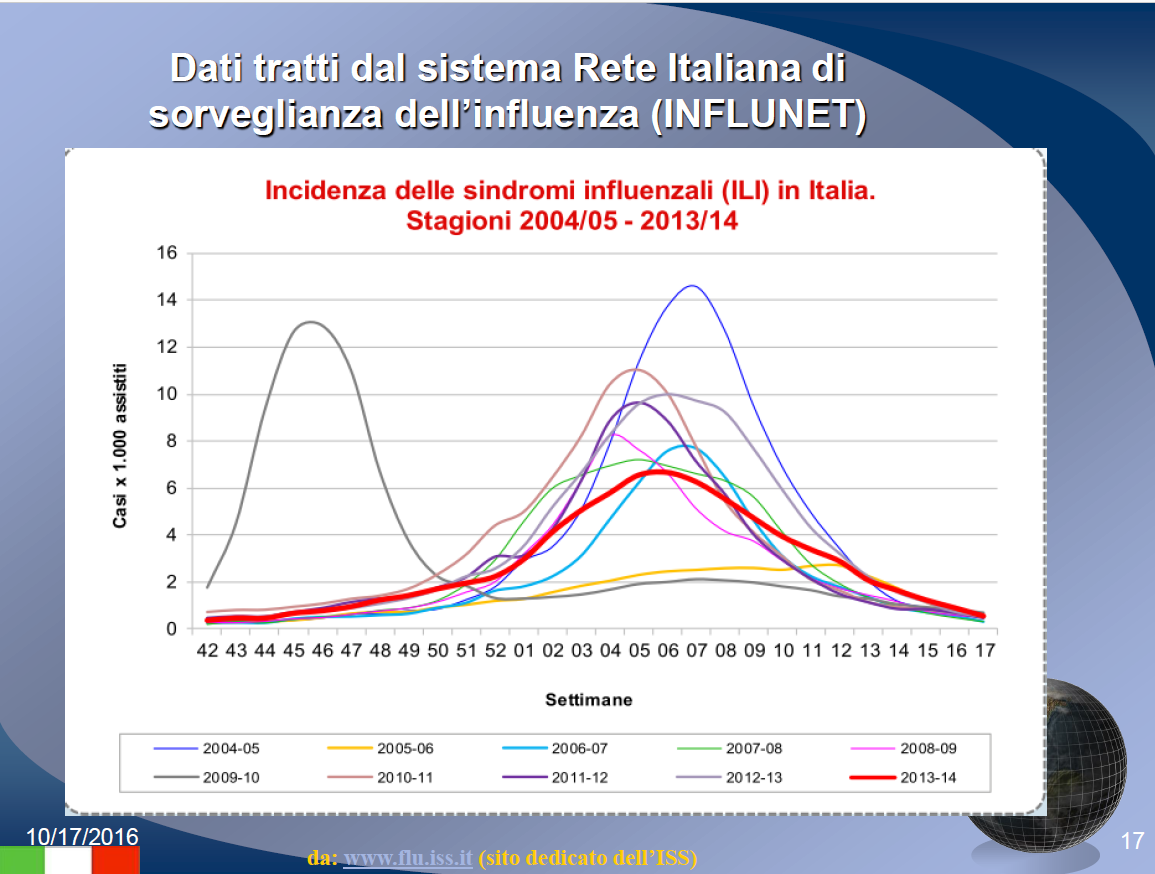
\includegraphics[width=0.9\textwidth]{02/image3.png}
\end{figure}


Ogni colore è una stagione invernale, anno per anno (per 10 anni) ci
disegna la frequenza delle sindromi influenzali in base alla settimana
dell'anno (1 -> 52). Cosa ci dice questo grafico?

Grossomodo, a prescindere dai picchi, in tutte le annate notiamo che
l'influenza comincia a diffondersi nelle ultime settimane dell'anno e
nelle prime 3-4 settimane del nuovo anno, quindi tra fine Dicembre ed
inizio di Gennaio e, termina a Marzo. Quindi la vaccinazione verrà fatta
entro l'inizio, ossia entro la metà di Dicembre.

Ci sono annate in cui il picco è più alto e altre in cui il picco è più
basso. Grossomodo nel decennio non notiamo un trend discendente o
ascendente. {[}Quando ci sono pochi cambiamenti antigenici, i soggetti
che hanno fatto la vaccinazione l'anno prima sono protetti, perchè c'è
la cross-reattività; ma quando arriva un virus nuovo i casi sono
maggiori.{]}

La curva grigia (anno 2009-2010) è l'anno in cui è arrivata la pandemia,
un nuovo virus con caratteristiche antigeniche completamente diverse,
con diversa distribuzione e il picco c'è stato a Novembre,
fortunatamente è stato un picco non acuto in termini di sintomi e di
gravità.

Dal punto di vista tecnico, con un grafico riesco a descrivere il
fenomeno in maniera molto chiara e molto semplice. L'epidemiologia ci da
anche qualche metodo per dimostrare i dati in maniera molto chiara. Una
raccolta di questo genere ci consente anche le differenziazioni per
fascia d'età.

Il sistema sentinella riporta il caso ma ne imposta anche le
caratteristiche.
\begin{figure}[!ht]
\centering
	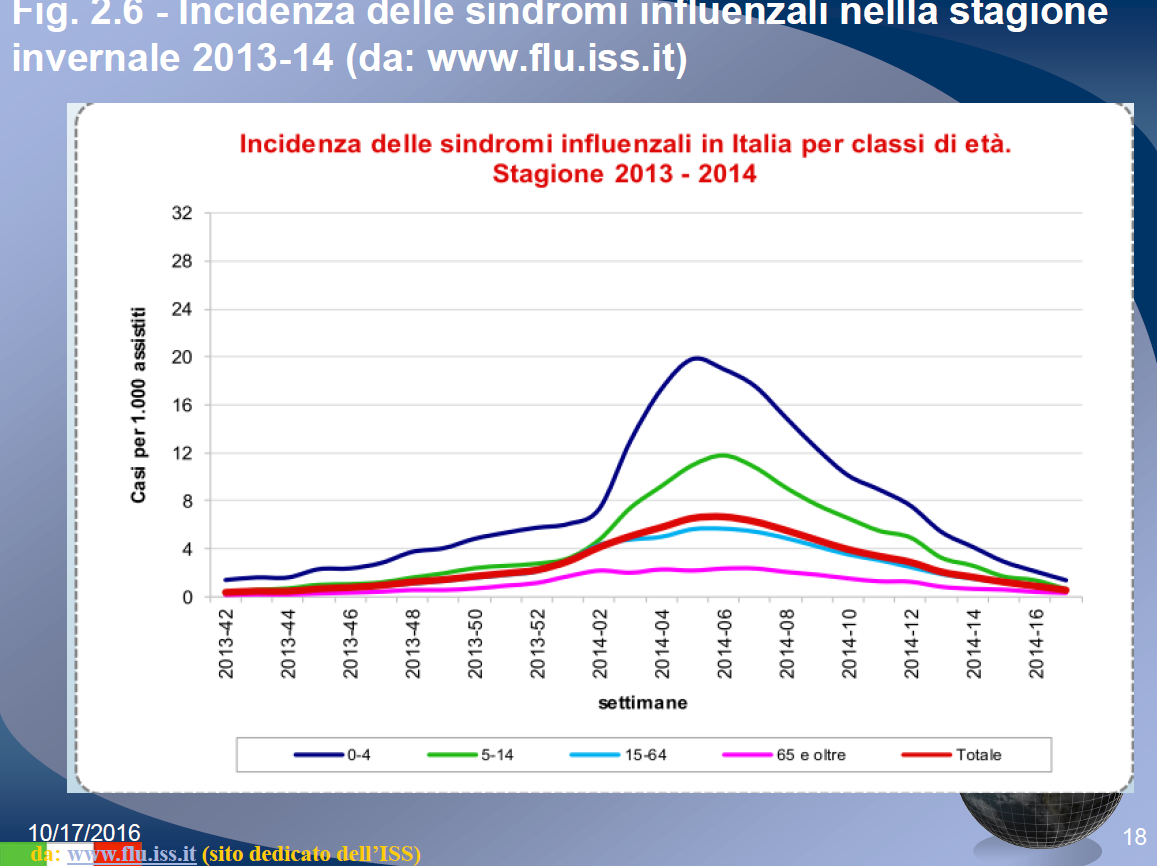
\includegraphics[width=0.9\textwidth]{02/image4.png}
\end{figure}


Distribuzione per un'annata (2013-2014) dei casi per fascia d'età. Si
nota che la fascia più colpita è quella infantile (0-4) seguita da
quella 5-14 anni.

Grazie ad una vaccinazione su larga scala fatta agli anziani,
l'influenza è più diffusa tra i bambini.

La vaccinazione si può fare nei bambini: negli USA è raccomandata a
tutti i bambini anche sani, in Italia è raccomandata solo ai bambini che
frequentano comunità affollate dove il rischio è maggiore.

\subsection{INDICATORI SANITARI}


Caratteristica di un individuo, di una popolazione o di un ambiente che
può essere quantificata ed è strettamente associata ad un fenomeno che
non è direttamente misurabile.

Es. Mortalità infantile \textgreater{} livello igienico

• Indicatori di sopravvivenza

• Indicatori dello stile di vita

• Indicatori di ``qualità di vita''

• Indicatori socio-economici

Indicatori sanitari, cosa sono? Gli indicatori sono dei dati, quasi
sempre epidemiologici, che misurano caratteristiche individuali o
collettive e che tendono a spiegare un fenomeno che non è direttamente
misurabile.

Se il fenomeno è lo stato di salute di una popolazione, devo trovare dei
dati che esemplifichino/quantifichino quel fenomeno che non è
direttamente misurato. Ho bisogno di dati oggettivi per misurare questo
stato di salute.

La \textbf{vita media} è un esempio di dato indicatore dello stato di
salute di una popolazione; se calcolo con le schede di morte che la vita
media della popolazione italiana è 81 anni, quella dell'Uganda è 55, c'è
in definitiva una bella differenza.

Quindi, l'indicatore sanitario misura un fenomeno.

L'indicatore non si ferma al dato sanitario. Ad es. c'è l'indicatore
economico che è il reddito medio della popolazione. Ogni dato va
contestualizzato e va valutata l'attendibilità.

La \textbf{mortalità infantile} è ancor più specifica della vita media
per valutare il livello igienico-sanitario di una popolazione. La
mortalità infantile è il numero di bambini morti nel primo anno di vita
diviso il numero di bambini nati vivi: alcune morti sono conseguenza di
malformazioni già presenti, altre sono legate a fattori ambientali; in
Italia è 5x1000, mediamente 5 bambini muoino nel primo anno di vita
rispetto a 1000 bambini nati vivi; nei paesi coi peggiori livelli
igienico-sanitari è 40x1000. Non sono considerate le morti fetali,
queste sono indicatori non dell'ambiente, ma dell'assistenza al parto.

\begin{figure}[!ht]
\centering
	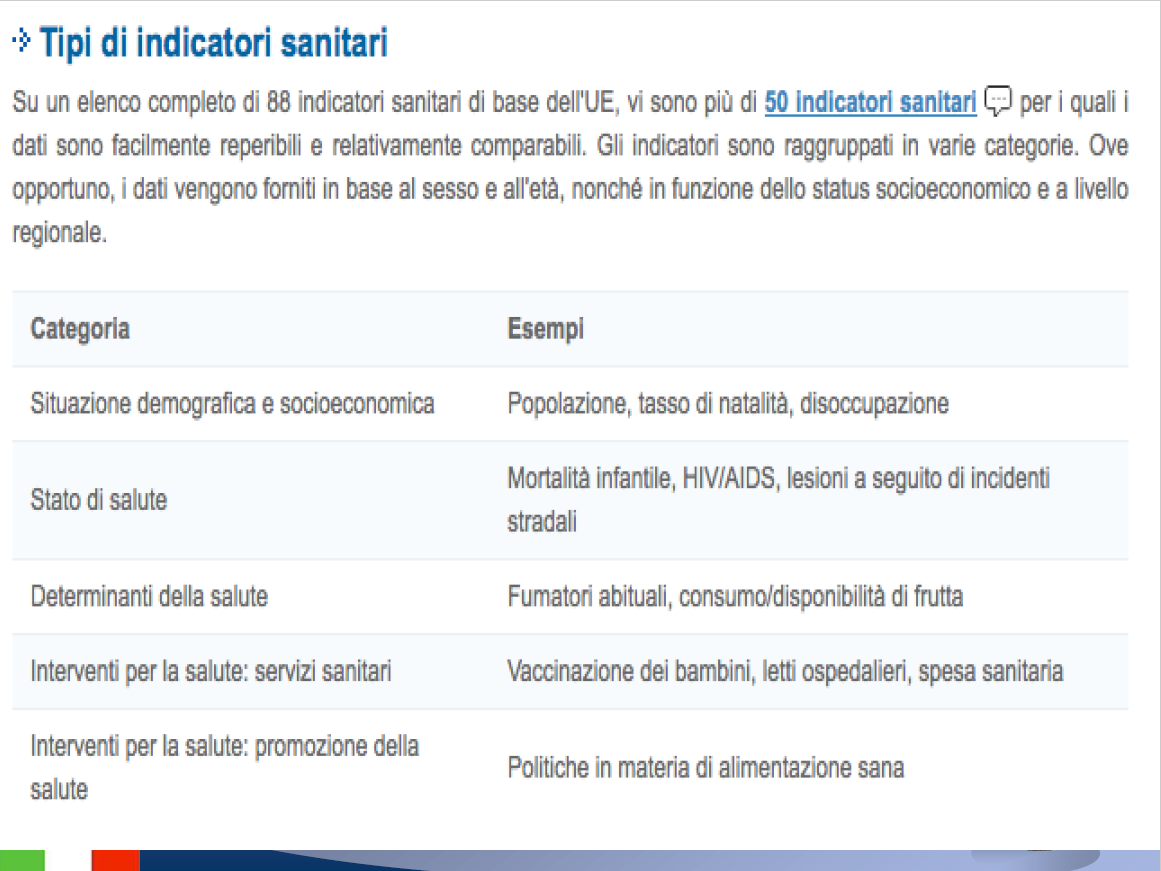
\includegraphics[width=0.9\textwidth]{02/image5.png}
\end{figure}


Abbiamo moltissimi indicatori sanitari su diversi ambiti; es. stato di
salute: mortalità infantile, incidenza di mortalità di AIDS, lesioni a
seguito di incidenti stradali. A seconda dell'obiettivo/studio/ricerca
possiamo prendere tutti i dati di cui abbiamo bisogno, usando le fonti
prima menzionate. Idem per i determinanti di salute, i fumatori, i
consumatori di alcool, percentuale di bambini vaccinati.

I dati abbondano, bisogna solo verificarne l'attendibilità, riordinarli
ed usarli per lo scopo della mia ricerca.
\begin{figure}[!ht]
\centering
	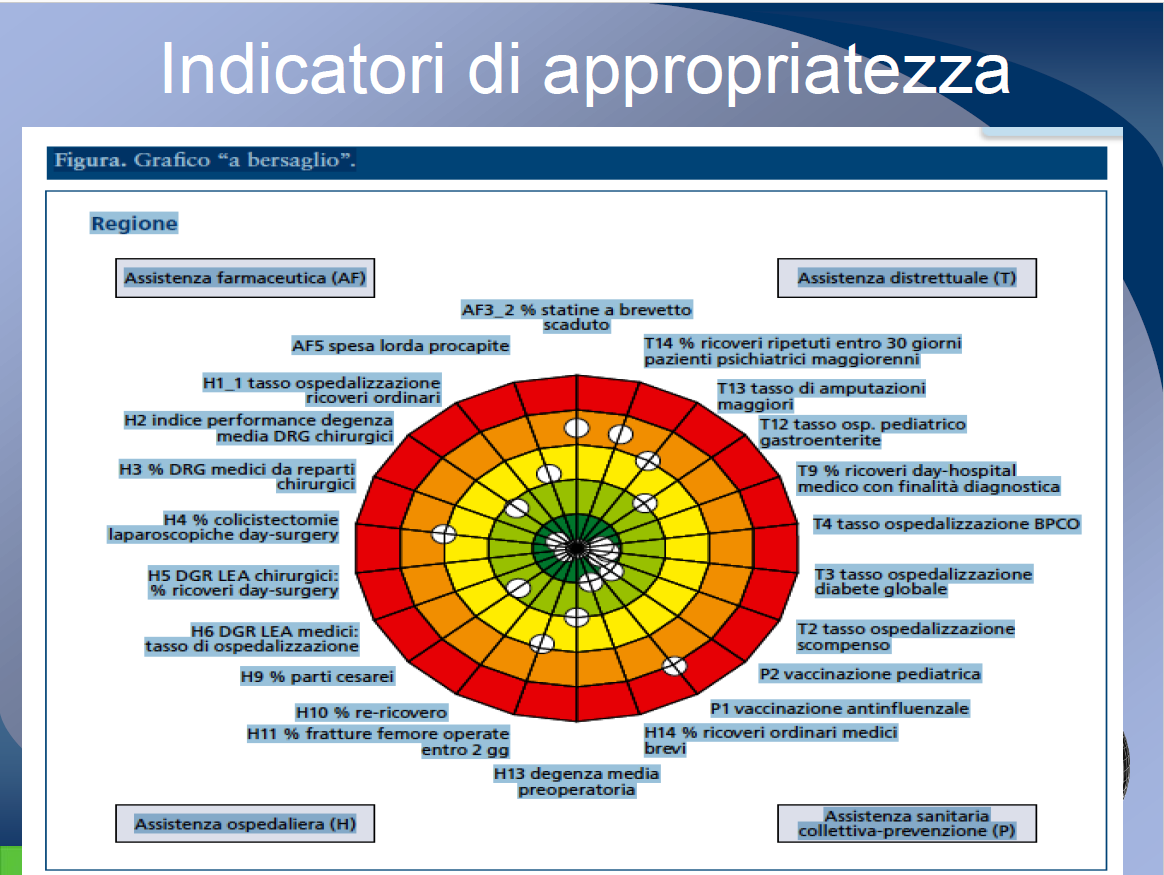
\includegraphics[width=0.9\textwidth]{02/image6.png}
\end{figure}


Trattamenti quali: degenza media pre-operatoria, frattura del femore
operato entro 2 giorni, \% dei parti cesarei, \% di colecistectomie
laparoscopiche in day surgery.

Sono tutti dati ed indicatori dell' assistenza sanitaria. Possiamo
vedere quali sono, regione per regione, le situazioni anomale rispetto
agli standard prestabiliti.

Qui non parliamo più di malattie, ma di assistenza sanitaria.
L'approccio è lo stesso.

\begin{figure}[!ht]
\centering
	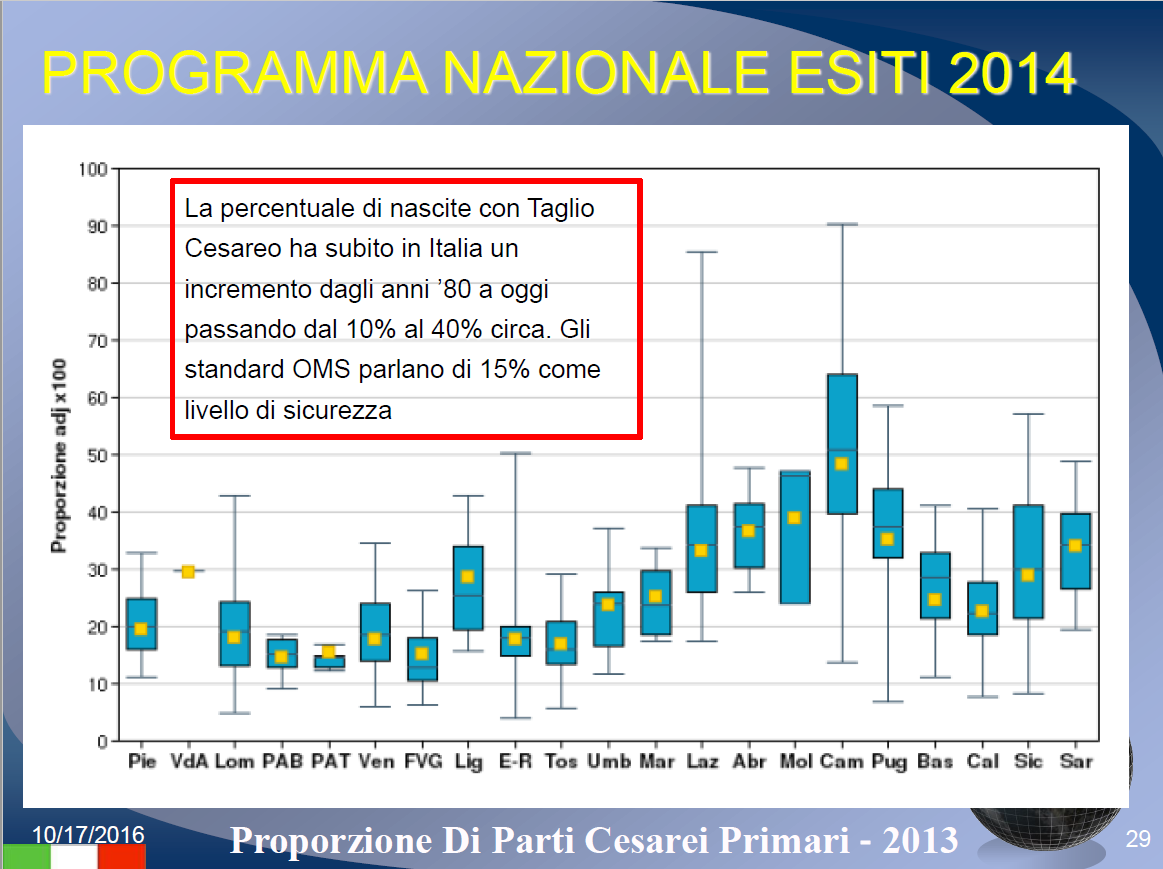
\includegraphics[width=0.9\textwidth]{02/image7.png}
\end{figure}


Queste sono le nascite con taglio cesareo nelle diverse regioni
italiane: un buon gruppo di regioni, soprattutto al Nord è sotto al
20\%, in altre regioni come la Campania si ha il 50\% di nascite con
taglio cesareo.

L'OMS ritiene che il 15\% di cesarei è sufficiente per far fronte a
quelle situazioni rischiose per la madre e per il feto. In Italia, negli
anni 80, la percentuale era del 10\%, ora siamo arrivati al 35\% ed è un
problema, perchè ciò comporta più costi e più complicazioni.

Ci sono una serie di motivi che lentamente hanno portato a questo
aumento di taglio cesareo, uno di questi è legato al non rischiare di
gestire dei parti complicati per via naturale preferendo la soluzione
del cesareo, perchè è più comodo, è più veloce e apparentemente più
sicuro (rischia meno il bambino, rischia più la madre). La mortalità
materna dopo taglio cesareo è 8 su 100.000; invece, la mortalità materna
dopo parto vaginale è 2 su 100.000. Ci sono 500.000 parti all'anno in
Italia, perdiamo almeno 30 donne morte dopo taglio cesareo: l'evento
accidentale è inevitabile dopo intervento chirurgico. Perchè succede
questo? Spesso è la partoriente a chiedere il parto con taglio cesareo,
firma e accetta il rischio; inoltre negli anni ci si è abituati a
gestire certe criticità col cesareo (presentazione podalica e parto
gemellare), si fa il cesareo e questa è diventata routine.

In Campania metà dei parti avvengono in strutture private non
accreditate, in tali strutture si va a prenotazione e si preferisce fare
un cesareo, perchè la durata è molto inferiore (30 minuti) rispetto al
parto per via vaginale (4-5 ore).

\subsection{Sistemi di sorveglianza sanitaria }

\begin{figure}[!ht]
\centering
	
\includegraphics[width=0.9\textwidth]{02/image8.png}
\end{figure}


Raccolta, attivazione, analisi dei dati seguiti dalla diffusione di
informazioni a tutte le persone potenzialmente interessate. Vi è una
sorveglianza di sanità pubblica, di luoghi di lavoro. La sorveglianza
sanitaria è un monitoraggio della situazione sanitaria con particolare
rilievo a qualche dato più importante, più sensibile di altro che
richiede interventi specifici e ad hoc.
\begin{figure}[!ht]
\centering
	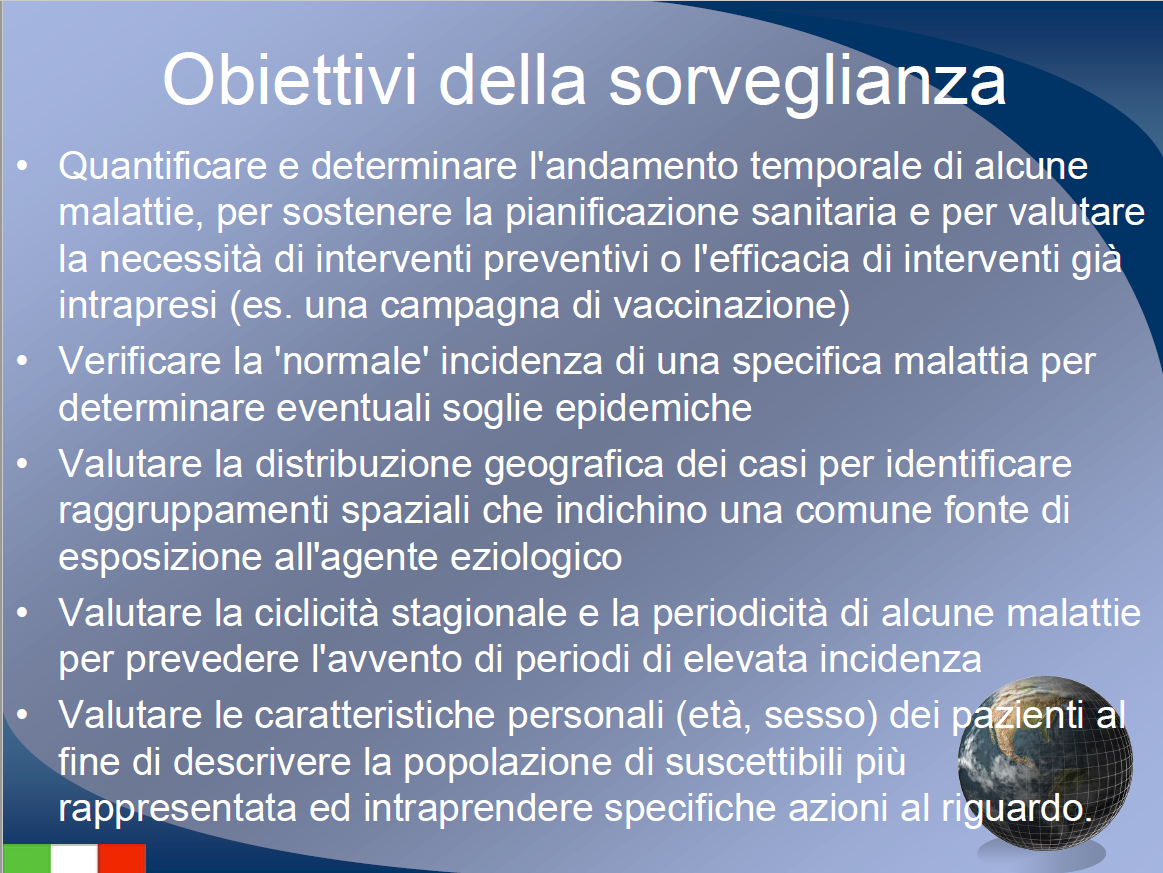
\includegraphics[width=0.9\textwidth]{02/image9.png}
\end{figure}


Obiettivi della sorveglianza: quantificare, determinare l'andamento
temporale di alcune malattie, verificare la normale incidenza,
verificare la distribuzione geografica, valutare la ciclicità
stagionale, valutare le caratteristiche personali. È una sorta di
``cruscotto'' che a livello locale, regionale, nazionale o
internazionale bisogna avere, perchè soprattutto per le patologie
infettive, dove sono più comuni i fenomeni epidemici, bisogna
intervenire laddove c'è un'anomalia notata in relazione al numero di
case. Le epidemie si identificano grazie alla sorveglianza sanitaria, se
non avessi il sistema delle notifiche non potrei dire che c'è in corso a
Parma l'epidemia di Legionellosi.
\begin{figure}[!ht]
\centering
	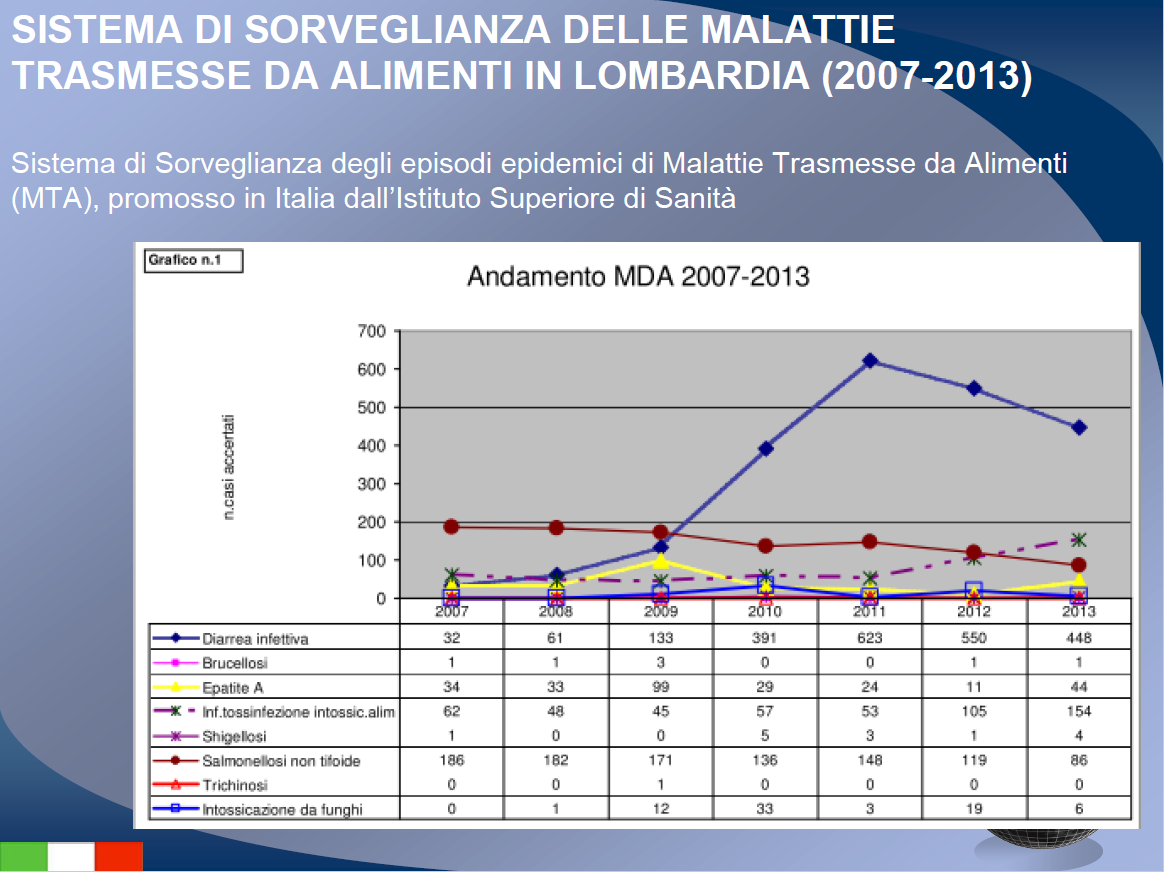
\includegraphics[width=0.9\textwidth]{02/image10.png}
\end{figure}


È un sistema di sorveglianza di malattie trasmesse da alimenti in
Lombardia: diarrea infettiva, brucellosi, epatite A, tossinfezione da
salmonella, trichinosi, intossicazione da funghi.

\begin{figure}[!ht]
\centering
	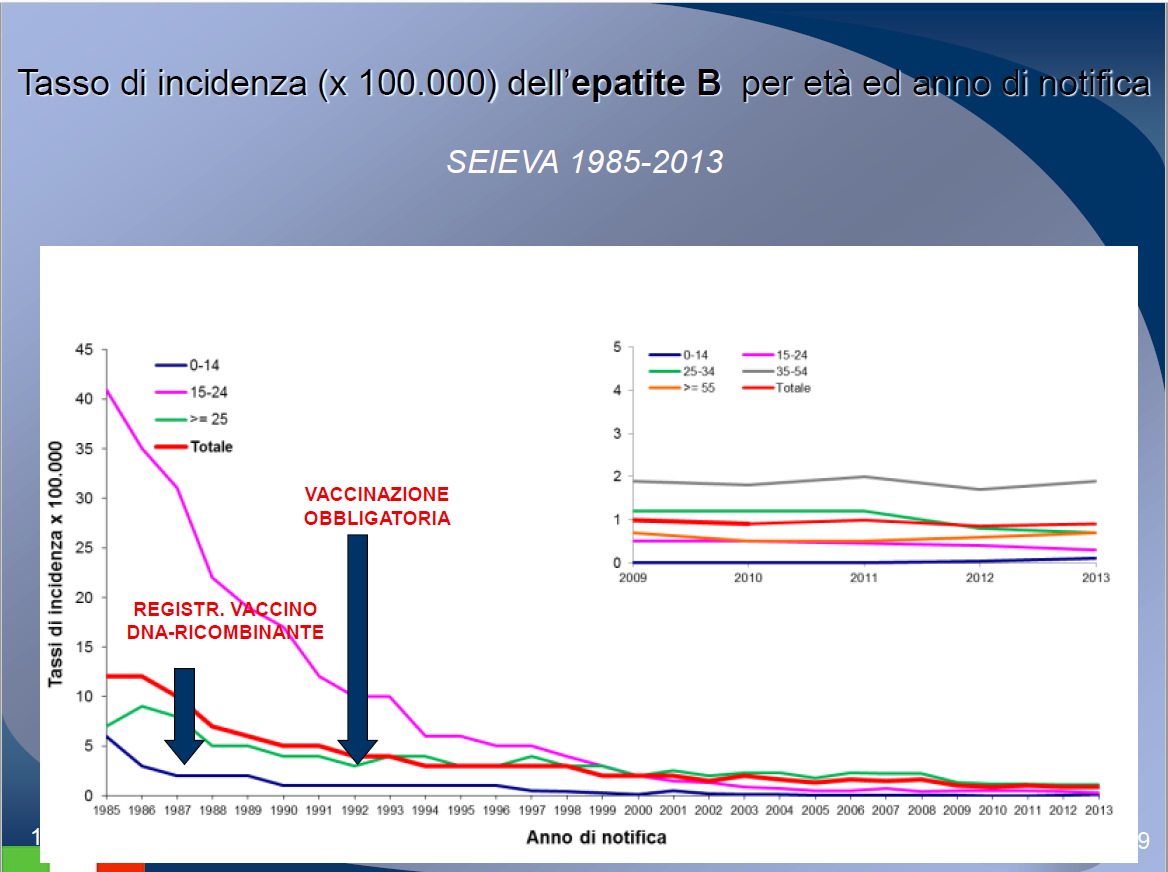
\includegraphics[width=0.9\textwidth]{02/image11.png}
\end{figure}


Sorveglianza dell'epatite B messa a punto dall'istituto superiore di
sanità. Questo grafico ci fa vedere che la malattia negli anni 80 già
scendeva, ma che è stato l'arrivo del primo vaccino nell'87 e del
vaccino obbligatorio nel 1992 che ha portato progressivamente ad una
diminuzione e quasi ad un azzeramento di casi.
\begin{figure}[!ht]
\centering
	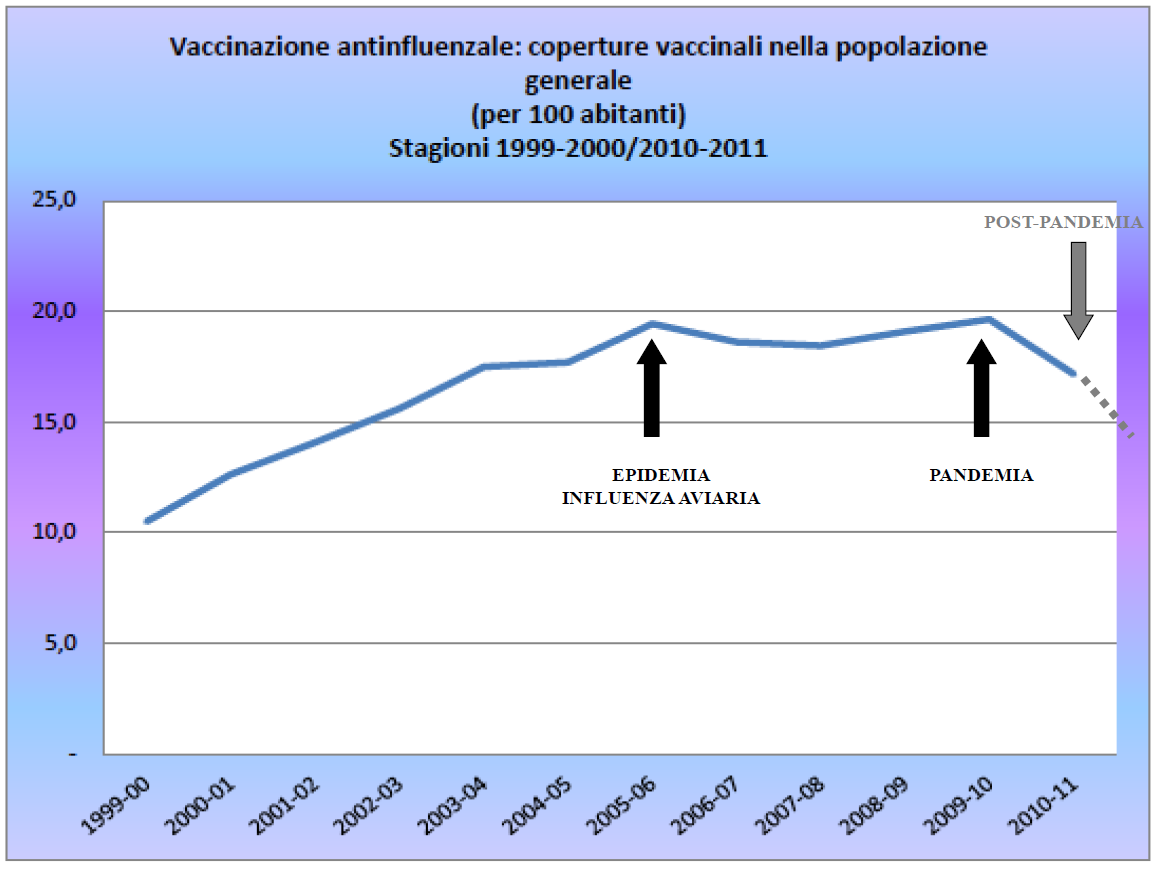
\includegraphics[width=0.9\textwidth]{02/image12.png}
\end{figure}


Andamento della vaccinazione antinfluenzale. Negli anni dell'epidemia
dell'influenza aviaria e nella pandemia c'è stata adesione più alta e
poi subito dopo dei cali di adesione alla vaccinazione.

Categorie raccomandate per la vaccinazione: malati cronici, ultra
65enni, bambini che frequentano comunità.

Gli operatori sanitari si vaccinano poco, non più del 15-20\%, questo è
un problema: in sé l'operatore sanitario non è un soggetto a rischio per
se stesso, ma può esser un rischio per i pazienti.
\begin{figure}[!ht]
\centering
	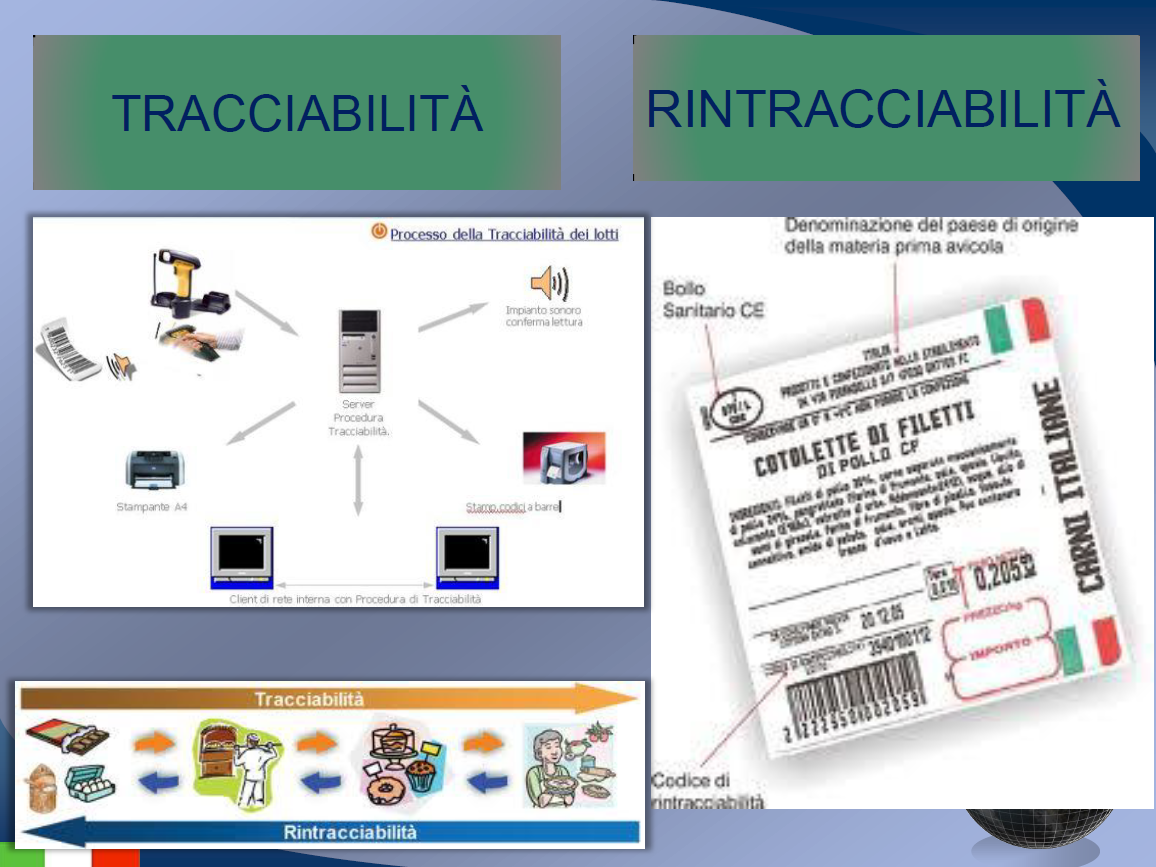
\includegraphics[width=0.9\textwidth]{02/image13.png}
\end{figure}


Sorveglianze per la tracciabilità alimentare con tutti i vari tipi di
controlli.

\begin{figure}[!ht]
\centering
	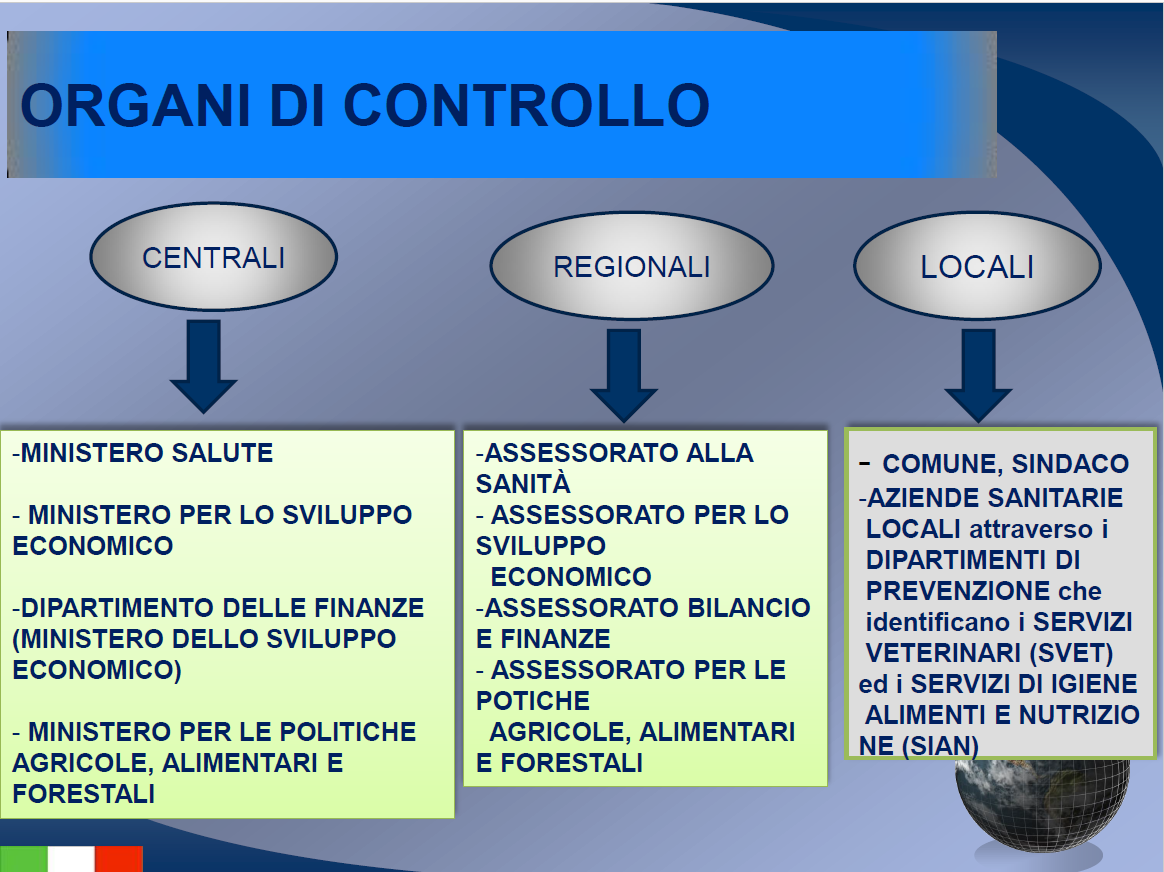
\includegraphics[width=0.9\textwidth]{02/image14.png}
\end{figure}


Il servizio sanitario nazionale non si occupa solo delle terapie e dei
ricoveri ospedalieri e in generale delle cure. Tutta questa filiera si
occupa dei controlli alimentari, questi sono un problema serio, in
Italia molto ben gestito che però mette in campo tutte queste strutture:
ministero della salute, ministero dello sviluppo economico, ministero
per le politiche agricole, forestale, alimentari, i vari assessorati
competenti nelle provincie e a livello locale; abbiamo da un lato le
aziende AUSL con i dipartimenti di prevenzione o i dipartimenti di
sanità pubblica, i servizi veterinari, i servizi di generi e alimenti
della nutrizione: tutti coinvolti nella filiera di verifiche, di
controlli a campione e di interventi in caso di problemi contingenti.

Qualche volta attivano i N.A.S. che sono un nucleo speciale dei
carabinieri specializzato nel settore sanitario, intervengono al bisogno
per ispezioni quando le autorità locali non ce la fanno o quando il caso
è talmente eclatante da dover indagare anche sulle mancanze
dell'autorità deputata al controllo, in questo caso si tratta di un
intervento ispettivo, è una anomalia, non è una routine. La routine
viene fatta attraverso questa filiera che parte dallo Stato e passa per
le regioni.
\begin{figure}[!ht]
\centering
	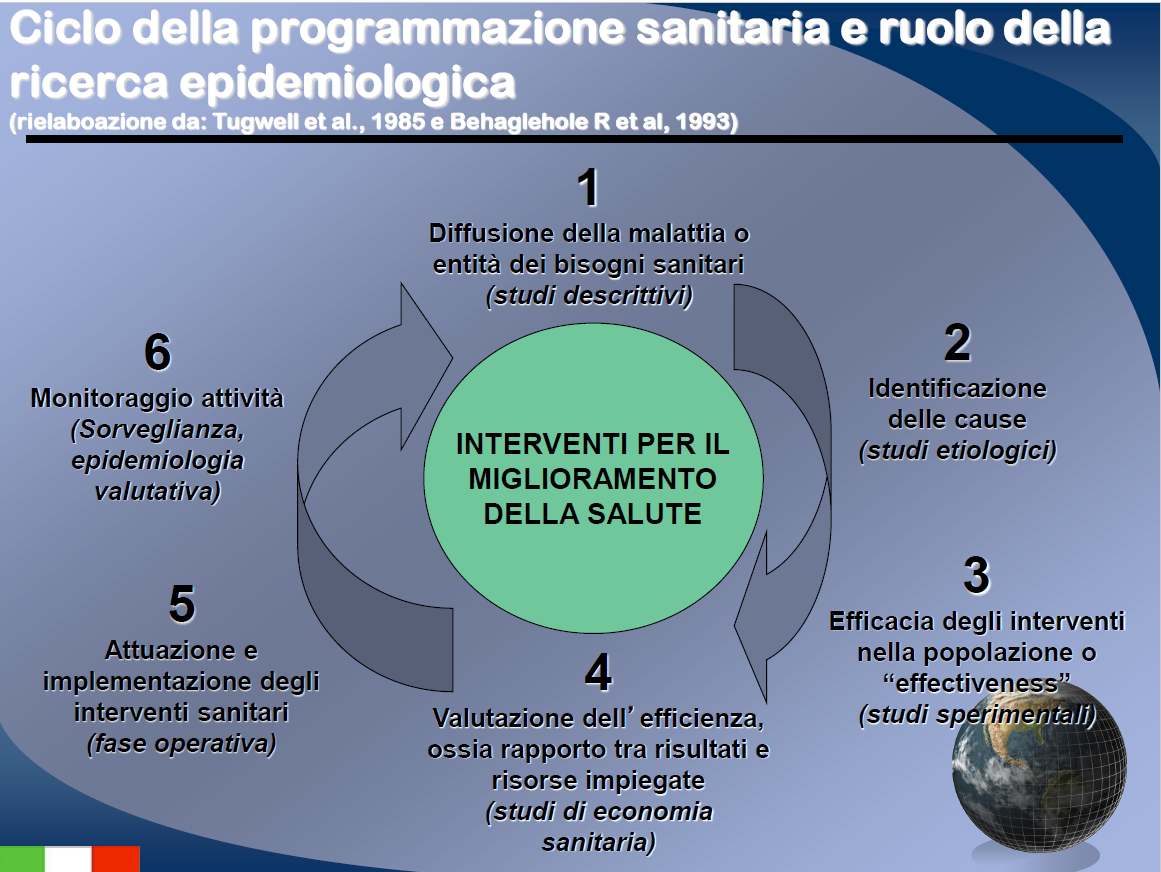
\includegraphics[width=0.9\textwidth]{02/image15.png}
\end{figure}


Questa diapositiva inquadra il ruolo dell'epidemiologia nella
programmazione sanitaria.

\textbf{1.} Per poter far bene la programmazione sanitaria bisogna
conoscere la situazione sanitaria e quindi bisogna conoscere la
distribuzione delle malattie e più specificamente quali sono i bisogni
sanitari di una popolazione che possono essere diversi tra una
popolazione e un'altra. In certi continenti abbiamo problemi sanitari
completamente diversi rispetto a quelli che abbiamo nel nostro paese. Se
facessimo programmazione sanitaria in Camerun e in tutti i paesi del
centro Africa ci dovremmo occupare in prima battuta di malaria,
HIV-AIDS, tubercolosi. Questi vengono chiamati ``the big killers'', sono
3 malattie infettive importanti per i quali non esiste di fatto la
copertura vaccinale: per la malaria è in sperimentazione ma non c'è il
vaccino, per l'HIV-AIDS se ne parla da 30 anni e non è mai arrivato, per
la tubercolosi c'è un vaccino poco efficace. Se facciamo programmazione
in Camerun abbiamo i 3 big killers che rappresentano i 3 obiettivi
principali; quindi avremo i dati di diffusione e dovremo occuparci di
come ridurre l'impatto di queste malattie. Fortunatamente in Italia non
abbiamo questi big killers, abbiamo queste malattie in quantità molto
ridotta, i nostri big killers sono altri: fumo, alcool, dieta; in
generale quei fattori di rischio che incidono sull'andamento delle
malattie più frequenti quali tumori e patologie cardiovascolari. Ciò
nonostante noi dobbiamo avere il quadro sanitario complessivo per poter
decidere quali sono le priorità.

\textbf{2.} Dobbiamo, dove possibile, identificare le cause; perchè se
conosciamo le cause delle malattie possiamo intervenire, se non le
conosciamo diventa tutto più difficile. Quindi, da un lato abbiamo gli
studi descrittivi che descrivono i fenomeni, dall'altro abbiamo quelli
eziologici o analitici che indagano sulle cause. Non basta dire che c'è
un eccesso di tumore al polmone, bisogna anche dire quali sono le cause
possibilmente removibili che determinano l'aumento di tumore al polmone;
qualche volta si può, altre non si riesce, dove non si riesce sarà
difficile ottenere buoni risultati in termini di riduzione della
malattia (se non conosco la causa).

\textbf{3.} e \textbf{4.} Valutare l'efficacia degli interventi
preventivi o curativi. Ci sono casi in cui devo applicare le migliori
terapie per scongiurare gli esiti di un fenomeno, caso eclatante è
l'epatite C: c'è un nuovo farmaco, è efficace, gli studi epidemiologici
confermano ciò, c'è un problema di costi; ma se riusciamo a dar le
terapie a tutti quei pazienti e questi le accettano risolviamo il
problema delle epatiti croniche con tutte le sequele che queste danno.
Qualche altra volta sperimentiamo i nuovi vaccini, sono sempre studi
sperimentali, se il vaccino è efficace lo si fa a tutti; in questo modo
andiamo ad incidere sull'incidenza della malattia in maniera diretta.

Dobbiamo fare lo sforzo, perchè il decisore sanitario (locale o
nazionale) ce lo chiede quasi sempre, di valutare il rapporto tra le
risorse impiegate e i risultati. L'epidemiologia ci da gli elementi per
farlo, lavora congiuntamente all'economia sanitaria che deve inserire i
computi economici del problema. Molta gestione in sanità è basata su
parametri economici: le terapie e i ricoveri costano; non abbiamo
risorse infinite da dedicare alla sanità.

\textbf{5.} È una fase operativa. Ho identificato il problema, ho
selezionato il metodo per ridurlo. La fase 5 lo attua cercando di
arrivare all'obiettivo di ridurre l'impatto di quella malattia.

\textbf{6.} Il sistema di sorveglianza deve essere in grado di dirci se,
dopo un congruo periodo (che dipende da situazione a situazione), si può
arrivare ad una situazione complessiva migliore.

Dunque, questa diapositiva ci fa capire come l'epidemiologia può aiutare
la programmazione sanitaria e in che modo leghiamo questi strumenti
utili e indispensabili per poter far bene l'approccio terapeutico.




\section{2a lezione di epidemiologia metodologica}

\subsection{Cronaca}


La Legionella è un microrganismo che si annida normalmente in tubature,
condutture, filtri. L'ipotesi che ci fosse la Legionella nelle torri di
raffreddamento è abbastanza plausibile. Non è però ancora chiusa
l'indagine. I casi sono diventati 38 ed i morti sono rimasti 2. I casi
ricoverati sono in via di miglioramento perchè la Legionella è sensibile
agli antibiotici. Ci devono essere un po' di accorgimenti per quanto
riguarda l'acqua, ma solo dal punto di vista delle vaporizzazioni,
perchè la Legionella ha una trasmissione aerea e non gastrointestinale.

La volta scorsa abbiamo parlato dei sistemi di sorveglianza e delle
fonti dei dati. Per quanto riguarda i dati, l'epidemiologia opera in due
direzioni:

\begin{enumerate}
\def\labelenumi{\arabic{enumi}.}
\item
  \textbf{APPROCCIO DESCRITTIVO} ai fenomeni sanitari
\item
  \textbf{APPROCCIO ANALITICO} dove l'epidemiologia è chiamata a
  identificare le cause ed i fattori di rischio
\end{enumerate}

Venendo all' esempio di Parma, il dato descrittivo è il numero di casi
di Legionellosi: 38. Questo numero però identifica il fenomeno
epidemico, ma non ci dice nulla su quelle che possono essere le cause.
Da che cosa deriva l'indagine epidemiologica analitica? Dal fatto che 35
di quei 38 casi erano concentrati in una determinata zona della città.
Questo porta ad identificare che in quell'area c'è un problema. Che
siano le torri o no, lo vedremo, ma il problema evidentemente è in
quell'area.

Nel 1874 a Londra ancora non si sapeva da cosa fosse causato il Colera e
così qualcuno diceva mangiando, altri bevendo, altri ancora respirando
quelli che venivano chiamati miasmi, cioè arie cattive maleodoranti. Ad
un certo punto, un medico di famiglia Inglese, il Dott. Snow, identificò
che la maggior parte dei casi si era verificata attorno ad una pompa
vicino a Piccadilly (non c'era ancora l'acqua corrente nelle case e si
andava ad attingere alle pompe in strada). Capì che i casi di Colera
derivavano dall'assunzione dell'acqua attinta da quella pompa. Si
identificò l'epidemia di colera 5 anni prima che fosse identificato a
Parigi, da Pasteur, il vibrione del Colera, che è l'agente eziologico.
Questo per dire che l'epidemiologia a volte identifica il problema anche
in assenza della conoscenza del meccanismo biologico. Nel caso della
Legionella si sa tutto e bisogna solo accertarsi che il patogeno sia in
quel determinato punto.

Quindi l'approccio \emph{descrittivo} sono le fotografie delle
situazioni: CHI, COSA ,QUANDO ,DOVE. Uno dei modi con cui affrontiamo
questo approccio può essere così definito: stima di nuovi casi di
tubercolosi per 100.000 all'anno, nelle diverse parti del mondo. Bisogna
ricordarsi che quando si scrive un lavoro scientifico, un rapporto, si
devono privilegiare le tabelle; quando si va ai congressi, si
privilegiano le diapositive. Come si può descrivere questa tabella?


\begin{figure}[!ht]
\centering
	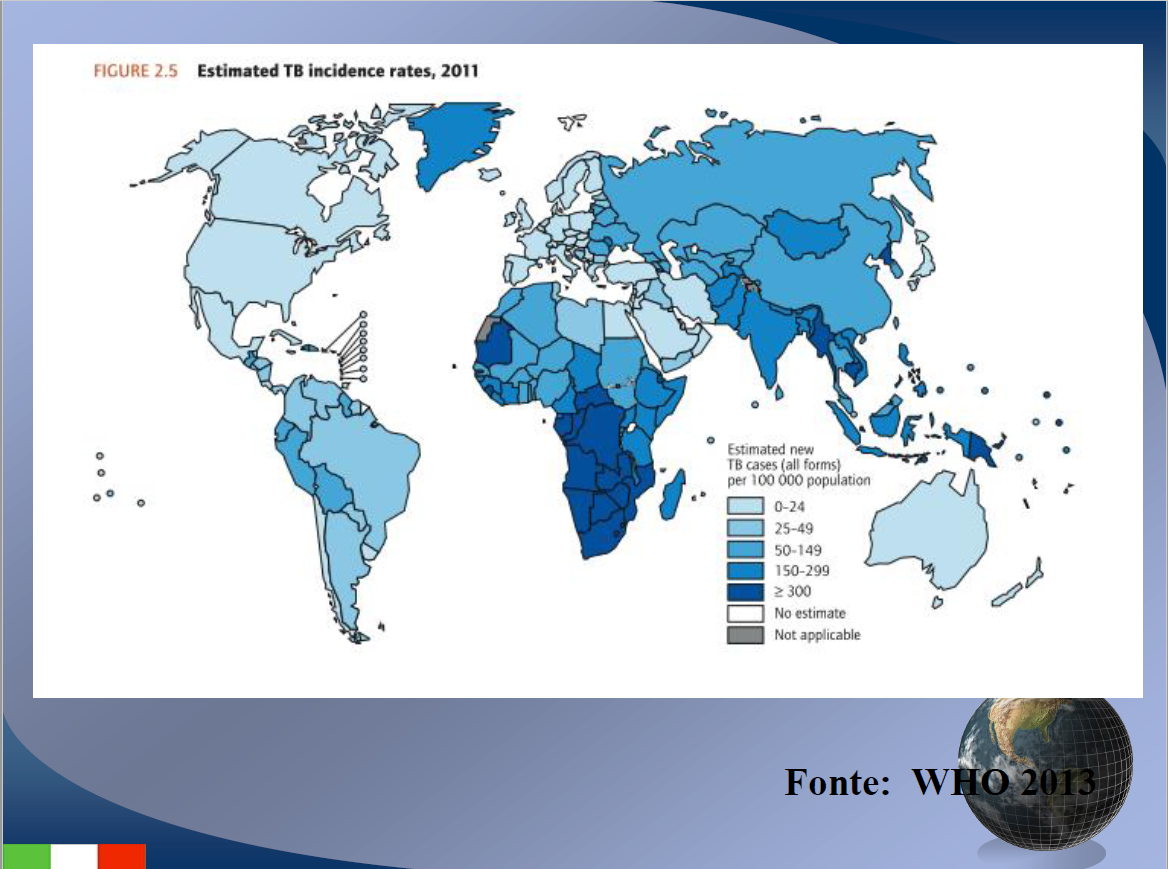
\includegraphics[width=0.7\textwidth]{03/image1.png}
\end{figure}

I paesi con più di 300 casi per 100.000 sono Africa Subsahariana,
qualche area del Sud est asiatico e la ex Unione sovietica. In realtà un
po' di TBC c'è in tutti i paesi del mondo. Non è una situazione
epidemica, ma endemica, con picchi diversi. Questo è il classico
approccio descrittivo al problema.

Se ci spostiamo alla seconda funzione dell' epidemiologia e cioè
all'approccio \emph{analitico}, andiamo a fare un'operazione leggermente
diversa , che è quella di identificare un'esposizione, che noi definiamo
così ma in realtà può essere una caratteristica individuale, una
genetica, un fattore di rischio o ambientale ecc. Generalmente noi
diciamo esposizione e misuriamo l'outcome e quindi l'effetto, cioè la
presenza e insorgenza della malattia. Di esempi ce ne sono tantissimi.

Ad es. \textbf{ESPOSIZIONE}: SINDROME METABOLICA, FATTORI EREDITARI,
ALIMENTAZIONE, SOVRAPPESO O OBESITA'-\/-\/-\/-\textgreater{}
\textbf{MALATTIA:} DIABETE.

Vedremo poi quali sono gli studi che ci permettono di fare questa
associazione, ma per il momento deve essere chiaro che l'approccio è
analitico.

Quando si va a valutare l'esposizione al fumo, si hanno dei risultati
così belli che i grafici vengono altrettanto bene a scopo didattico. In
questo caso abbiamo:

\begin{figure}[!ht]
\centering
	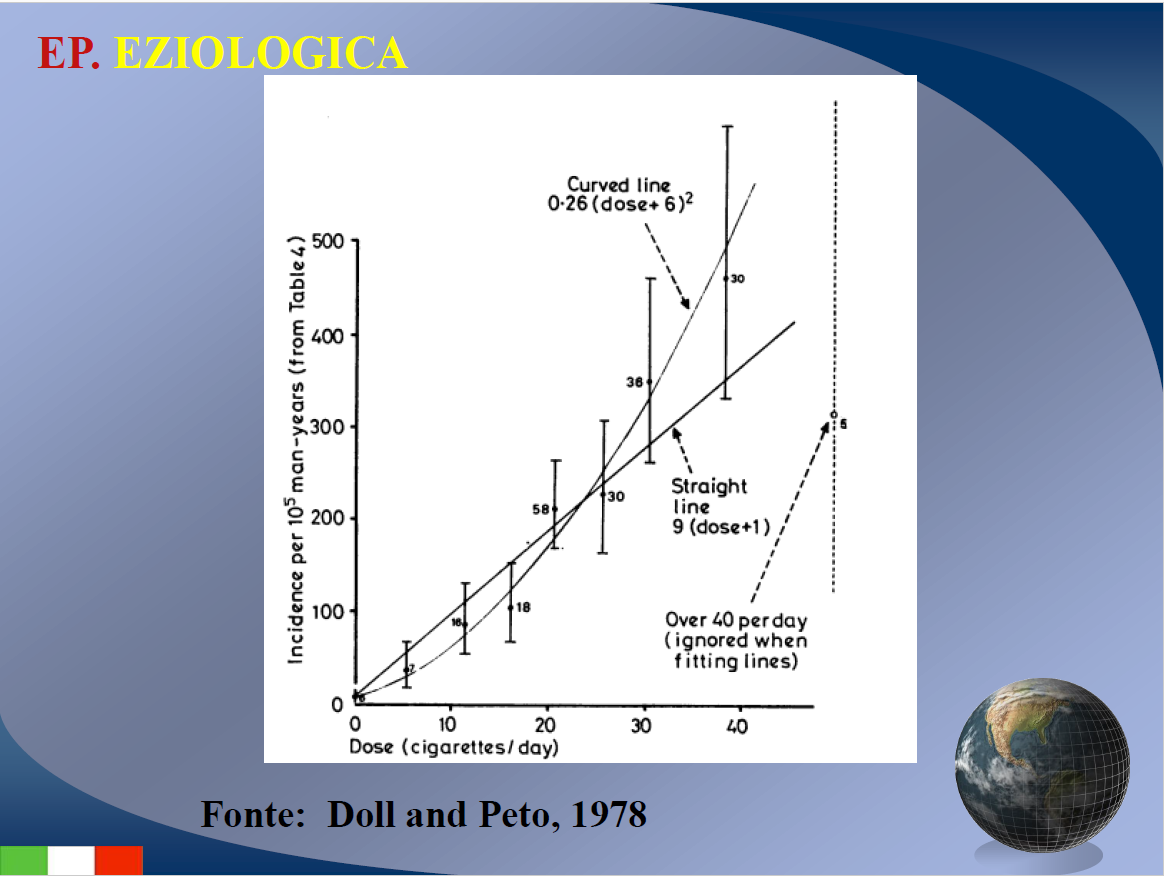
\includegraphics[width=0.7\textwidth]{03/image2.png}
\end{figure}

Sull'asse delle ascisse il numero di sigarette al giorno e in ordinata
l'incidenza, quindi la frequenza delle malattie cardiovascolari x $10^5$. I
puntini e le linee rappresentano i valori ed i limiti di confidenza. Le
rette sono le rette di correlazione. Al di là dei tecnicismi noi vediamo
che all'aumentare dell'esposizione, c'è un aumento dell' outcome e
quindi del rischio cardiovascolare.

Nei fattori di rischio c'è sempre una correlazione lineare
DOSE-RISPOSTA? Quasi sempre. Normalmente più siamo esposti, più
rischiamo, con qualche eccezione però. Ad esempio l'alcool. Se misuriamo
l'alcool e gli effetti cardiovascolari, notiamo che per piccole quantità
di alcool assunto, non solo non c'è effetto aggravante, ma addirittura,
per una ragione legata alla presenza di un maggior numero di
lipoproteine ad alta densità, l'alcool a modiche esposizioni può essere
un fattore protettivo per gli eventi cardiovascolari maggiori. Per
piccole quantità si intende mezzo bicchiere di vino a pasto. In questo
caso avremo una curva a U e non una retta lineare. Avremo che, per
piccole quantità, ci sarà un calo del rischio, via via salendo, un
rischio aumentato.

\subsection{Misure di frequenza di malattia}


\begin{figure}[!ht]
\centering
	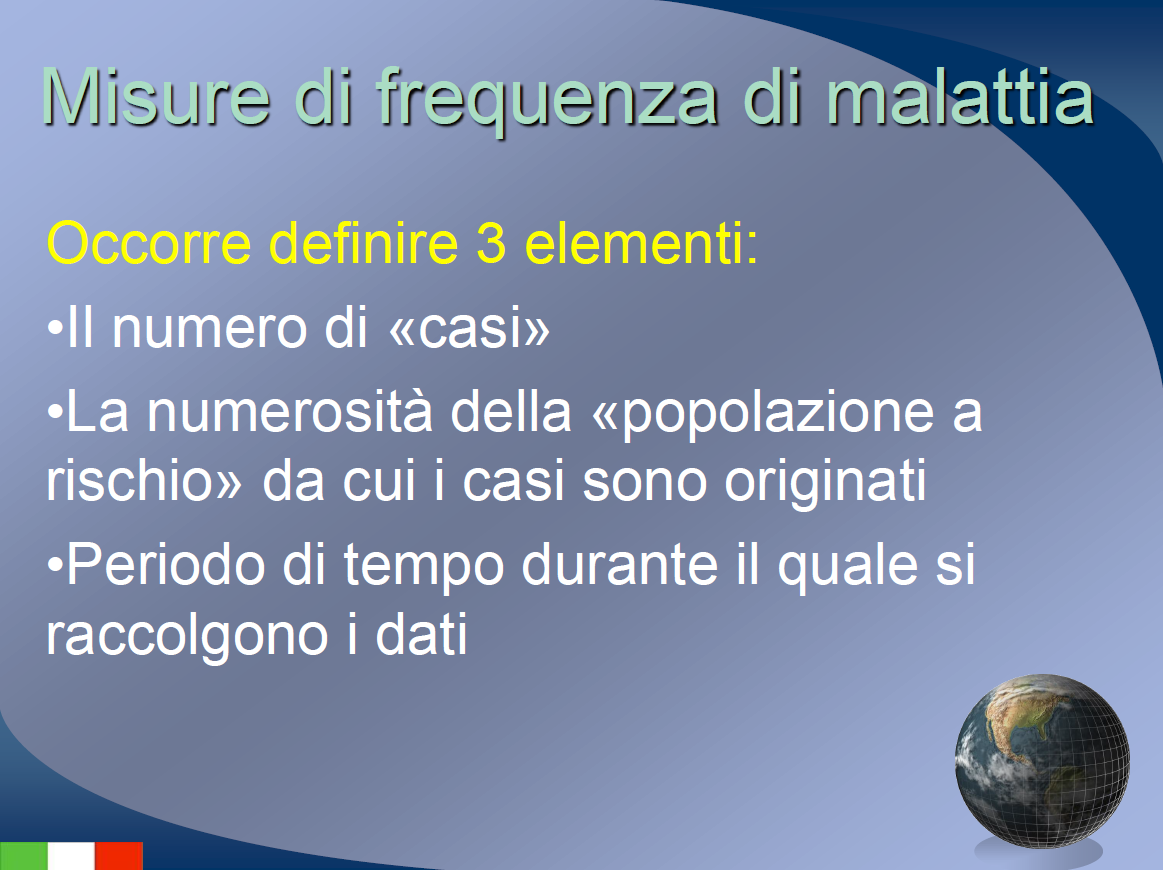
\includegraphics[width=0.7\textwidth]{03/image3.png}
\end{figure}

Vediamo ora quali sono le \textbf{misure di FREQUENZA} di un EVENTO
SANITARIO che per comodità qui chiamiamo malattia, ma potrebbe essere
morte, insorgenza di sintomi e così via.

Normalmente, misuriamo il numero di eventi in questo modo: numero di
nuovi casi per 100.000 abitanti, ma ci deve essere l'unità temporale che
nella maggior parte dei casi, per le misure epidemiologiche, è un anno .
Non è però sempre così, perchè, se misuriamo una tossinfezione
alimentare, abbiamo un periodo di incubazione talmente breve, che
potremmo calcolare l'incidenza settimanale o giornaliera. Più
frequentemente però, i dati epidemiologici, hanno l'incidenza annua.

\begin{figure}[!ht]
\centering
	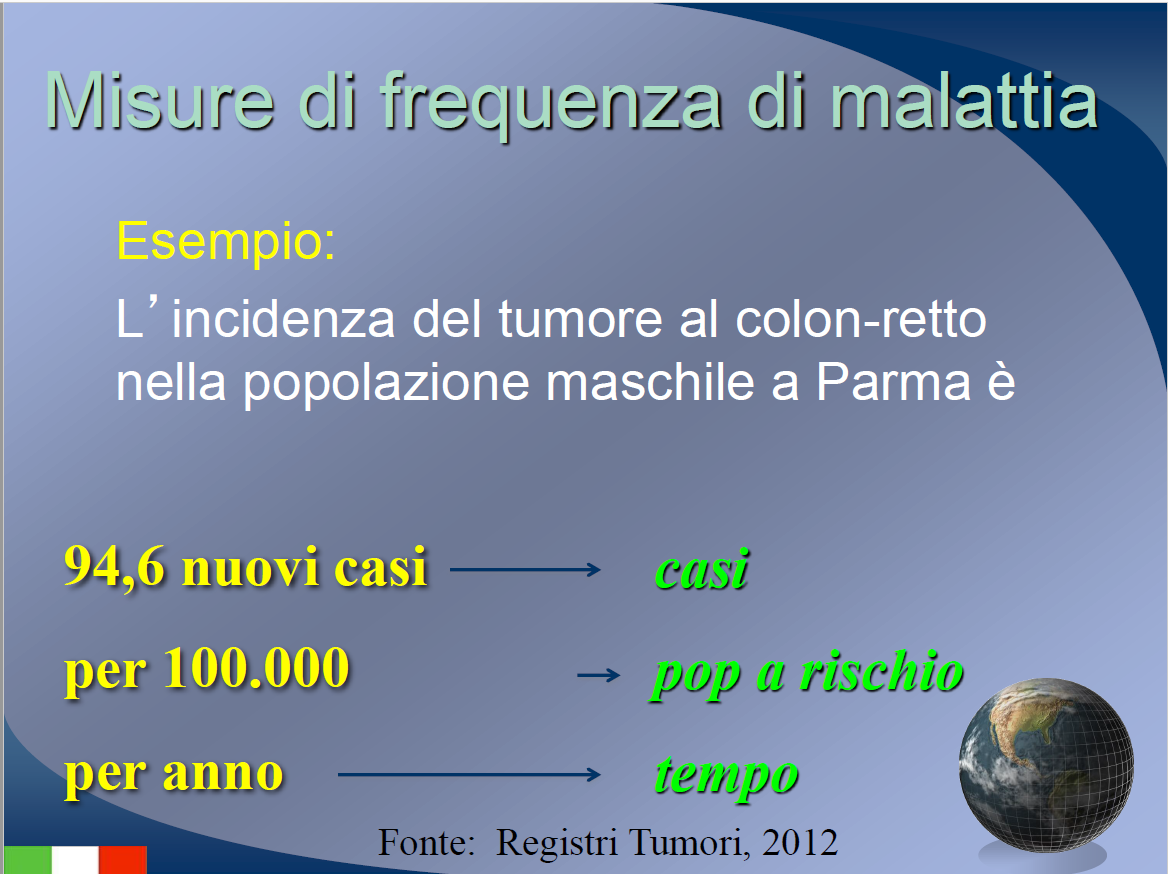
\includegraphics[width=0.7\textwidth]{03/image4.png}
\end{figure}

Questo dato, tratto dal registro dei tumori di Parma, significa che,
ogni anno, abbiamo 94,6 casi di tumore al colon-retto per 100.000.
Quindi, se la provincia di Parma ha più o meno 400.000 abitanti, ci
aspettiamo più o meno circa 379 casi di tumore al colon. Questo è un
dato descrittivo che ha una duplice funzione: da un lato valutare
l'incidenza e vedere se nel tempo sale, scende o rimane uguale;
dall'altro è utile per sapere cosa aspettarci,ovvero che la rete
ospedaliera di Parma deve essere pronta a gestire ogni anno 379 casi di
tumore al colon retto. Può sembrare una cosa non rilevante ,ma è invece
fondamentale per organizzare le chirurgie. Si spera sempre che i casi
scendano, ma potrebbero anche salire e nel caso del colon-retto i casi
sono in continua ascesa. Perchè? Una parte è legata al fatto che sta
aumentando la popolazione anziana e questo è un tumore che tende a
svilupparsi nell'età avanzata (ha il suo picco a 60 anni); un'altra è
legata all'introduzione di un elemento più raffinato per il quale oggi
contiamo più casi: lo SCREENING, la diagnosi precoce; ed infine ci sono
fattori di rischio che incidono e fanno aumentare questa patologia.

Esiste oggi un programma di screening per la ricerca di tumore al
colon-retto che si effettua tramite la ricerca di sangue occulto nelle
feci ed è richiesto dai 50 ai 70 anni con frequenza biennale. Andando a
fare centinaia o migliaia di questi test, ogni tanto trovo un tumore non
diagnosticato e ancora in fase precoce. Alla ricerca del sangue occulto,
se positivo, segue la colonscopia. Identificato il tumore, lo opero.
Ovviamente questo conta uno come caso, ma ha una prognosi decisamente
migliore rispetto a quando il paziente viene perchè ha dei sintomi. Così
però, mi aumenta l'incidenza. Quando inizio un programma di screening
devo mettere in conto che avrò un aumento dell'incidenza e che questo è
un artefatto, dovuto al fatto che anticipo la diagnosi. C'è anche
qualcuno che si chiede: se identifico un tumore di 1 cm, siamo certi che
questo maturerebbe fino a dare dei sintomi e porterebbe a morte il
paziente? Questo non si sa. Però se trovo un tumore maligno lo devo
eliminare. Anche perchè c'è un rischio di metastasi che è direttamente
proporzionale alle dimensioni della neoplasia, quindi prima la prendo,
più piccola è, migliore sarà la prognosi. Questo vale anche per la
diagnosi precoce del tumore al seno. Tutto ciò fa lievitare l'incidenza
dei tumori. Però qualcosa di positivo c'è perchè, mentre sale
l'incidenza del tumore al colon-retto, la mortalità cala.

Vediamo le \textbf{MISURE DI FREQUENZA} di una malattia.

Se misuriamo il numero assoluto di casi, questo non ci da risposte per
poter fare un'analisi comparativa con altri paesi. Abbiamo bisogno di un
denominatore. Contare i casi di per sè interessa poco, a meno che non si
tratti di una situazione come l'epidemia di legionellosi, in cui
normalmente la base è zero casi e quando inizio ad averne 10, 20, 30, mi
rendo conto dell'impatto che può avere la patologia. Normalmente si
lavora con due misure:

\begin{enumerate}
\def\labelenumi{\arabic{enumi}.}
\item
  \textbf{INCIDENZA:} \emph{numero di nuovi casi in un intervallo di
  tempo prestabilito}.
\end{enumerate}

E' una misura dinamica. Se vogliamo complicarci le cose, dobbiamo fare
un'ulteriore precisazione. Dobbiamo parlare di \textbf{INCIDENZA
CUMULATIVA e TASSO PERSONA-TEMPO.}
\begin{figure}[!ht]
\centering
	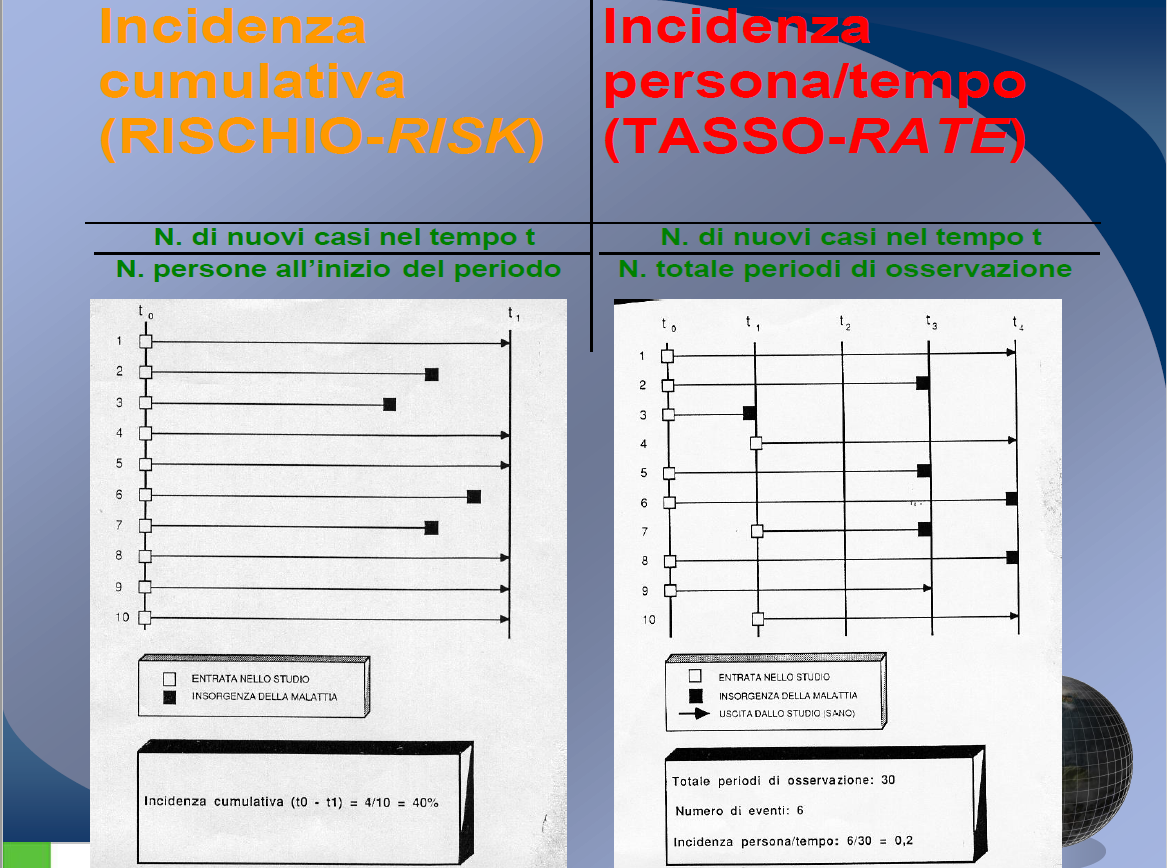
\includegraphics[width=0.7\textwidth]{03/image5.png}
\end{figure}

Il caso più semplice (incidenza cumulativa) mostra: 10 persone (il
numero è indifferente), un intervallo di tempo e un numero di casi che
insorgono in quel periodo. In questo caso 4 su 10 =\textgreater{} numero
di nuovi casi 4, persone all'inizio 10, incidenza del 40\%
nell'intervallo, che facciamo conto sia un anno. Un caso del genere si
ha quando prendiamo un numero limitato di soggetti, li seguiamo
dall'inizio di una certa età, data una certa esposizione ecc.. è un
gruppo chiuso di pazienti. Quando noi lavoriamo sulla popolazione però,
non abbiamo mai a che fare con gruppi chiusi, perchè in una popolazione
c'è gente che muore, che nasce, che migra. Non ho mai un denominatore
fisso e bloccato e allora devo fare un'operazione di approssimazione:
anzichè valutare X soggetti e il numero di casi in quei soggetti, valuto
le unità di tempo. Quindi il soggetto A ce l'ho per 4 anni
-\/-\/-\textgreater{} 0 casi per 4 anni. Nel secondo caso ho che, al
terzo anno, insorge la malattia. In realtà ho avuto la persona a rischio
per 3 anni, ma quando si ammala non è più a rischio di riammalare perchè
di solito la malattia si prende una volta sola: malattia
infettiva-\/-\/-\textgreater{} sviluppo l'immunità, malattia
cronica-\/-\/-\textgreater{} quando la prende ce l'ha per sempre. Noi
lavoriamo facendo il numero di nuovi casi diviso per il periodo di
osservazione. Quindi il dato di incidenza è quello che viene fuori nelle
statistiche perchè, quando lavoro su una popolazione, non ho mai la
coorte stabile. Tanto è vero che per calcolare il denominatore delle
popolazioni si usa il dato al 30 giugno e non al 1 gennaio o al 31
dicembre, perchè se c'è un movimento demografico, andando a prendere a
metà del periodo, ho una buona approssimazione di quante sono le persone
a rischio in quell'anno. I movimenti demografici normalmente sono lenti,
però, per essere precisi, scelgo quel periodo. Quindi alla fine avrò
incidenza persona-tempo, numero di casi, divido a periodi e lo 0,2
(della diapositiva in alto, incidenza persona-tempo) significa 20\%. Ma
rispetto a cosa? non alle persone, ma rispetto all'anno. Quindi ciascun
soggetto sano che sta un anno, ha il rischio del 20\% di sviluppare la
malattia. Il concetto non cambia, è solo un modo diverso di applicare il
tasso di incidenza. Questi dati sono di mortalità: incidenza intesa come
morte non come casi di malattia. Il tasso di mortalità non è altro che
un tasso di incidenza in cui l'evento non è l'insorgenza della malattia
ma è la morte del soggetto. Noi diciamo tasso e questo evoca un
interavallo temporale. Siamo nell'ambito dell'epidemiologia descrittiva.

\begin{figure}[!ht]
\centering
	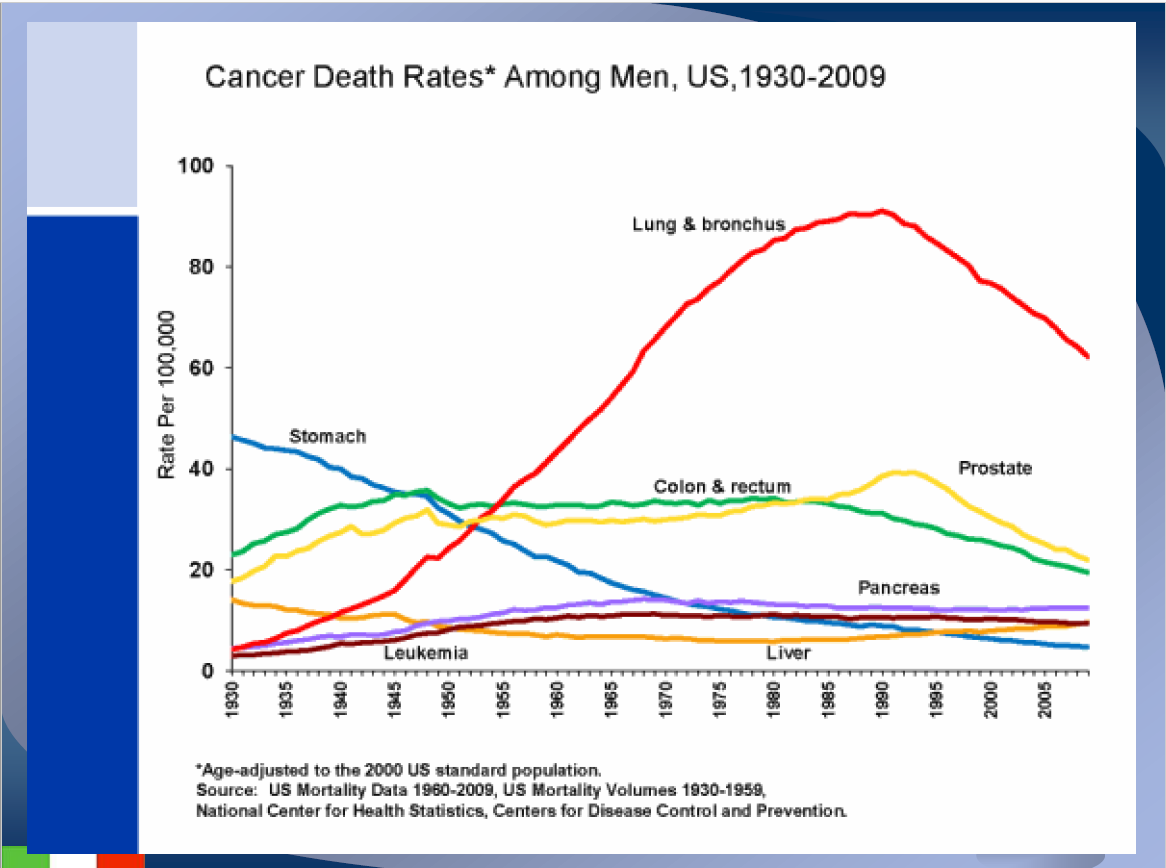
\includegraphics[width=0.7\textwidth]{03/image6.png}
\end{figure}

Questo dato, riferito agli Stati Uniti, ci dice il tasso di mortalità
per singoli tumori. Dal 1930 al 2010 vediamo un grande picco di tumori
polmonari che poi è andato calando dagli anni '90 in poi. Notiamo un
calo drastico del tumore allo stomaco dagli anni '30. I dati di
mortalità sono più attendibili e vanno indietro nel tempo molto più dei
tassi di incidenza, maggiormente difficili da calcolare, perchè mentre
sulla fonte dei dati la scheda di morte c'è sempre, sull'incidenza
potremmo non avere tutti i dati. Per il colon-retto notiamo un calo, ma
stiamo parlando di mortalità. Se avessimo i dati di incidenza, noteremmo
un aumento. Leucemia e tumore al pancreas sono in crescita. Il tumore
alla prostata ha un andamento ondulante.
\begin{figure}[!ht]
\centering
	
\includegraphics[width=0.7\textwidth]{03/image7.png}
\end{figure}
E' sempre bene avere presente il numero di casi, ma non bisogna
focalizzarsi solo su quelli, bensì sull'incidenza. E perchè questo?
Perchè ci fa capire che, se mettiamo insieme le mortalità per cancro
(questi sono dati australiani), possiamo avere numero assoluto in
aumento e l'incidenza in diminuzione. A noi non interessa il numero
assoluto perchè, se aumenta la popolazione, avremo più casi e non è
detto che ci sia un'incidenza maggiore. Dunque, in teoria, se la
popolazione rimanesse la stessa, il numero di casi avrebbe un trend
identico all'incidenza, ma siccome la popolazione cambia, si può vedere
la situazione in cui il numero di casi aumenta e l'incidenza diminuisce.
A quale credere? se sto facendo lo studio epidemiologico devo guardare
l'incidenza, ma se sto organizzando i servizi sanitari per curare i
malati, mi interessa il numero assoluto.

\begin{quote}
\textbf{2. PREVALENZA:} \emph{rapporto tra i casi esistenti e la
popolazione totale}.
\end{quote}

L'incidenza è un film, non è una misura istantanea, perchè devo sempre
avere un riferimento temporale. Non ci può essere un'incidenza puntuale.
Ci deve sempre essere la misura tempo che convenzionalmente per le
malattie è l'anno. Un po' come quando misurate la velocità. Misurate
km/h, m/s, c'è sempre l'intervallo temporale. La prevalenza invece è una
fotografia istantanea e fotografa la situazione esistente: numero di
casi di malattia, numero di esposti ai fattori di rischio...

Se faccio alzare la mano qui dentro a chi ha il raffreddore e mi alzano
la mano in 10, mettiamo che siete in 100 -\/-\/-\textgreater{} ho la
prevalenza del raffreddore del 10\%. Altro esempio: chi fuma? si alzano
25 mani. In questo caso ho la prevalenza del 25\%.

Classico dato di prevalenza: nell'annuario statistico 2012 si indica che
è diabetico il 5,5\% degli Italiani, valore leggermente più alto nelle
donne rispetto agli uomini; o ancora, secondo uno studio dell'OMS il
25\%-79\% degli adulti risulta in sovrappeso e il 5-30\% obeso. Sono
fotografie istantanee delle situazioni che hanno un loro significato di
rilievo istantaneo, che può essere ripetuta nel tempo. Se io fotografo
la situazione del sovrappeso in diversi anni, potrei arrivare a scoprire
differenze di un certo significato. Ad es .dagli anni '80 agli anni
2000, il sovrappeso è aumentato con tutte le conseguenze che esso può
comportare. Questo è un dato di prevalenza.
\begin{figure}[!ht]
\centering
	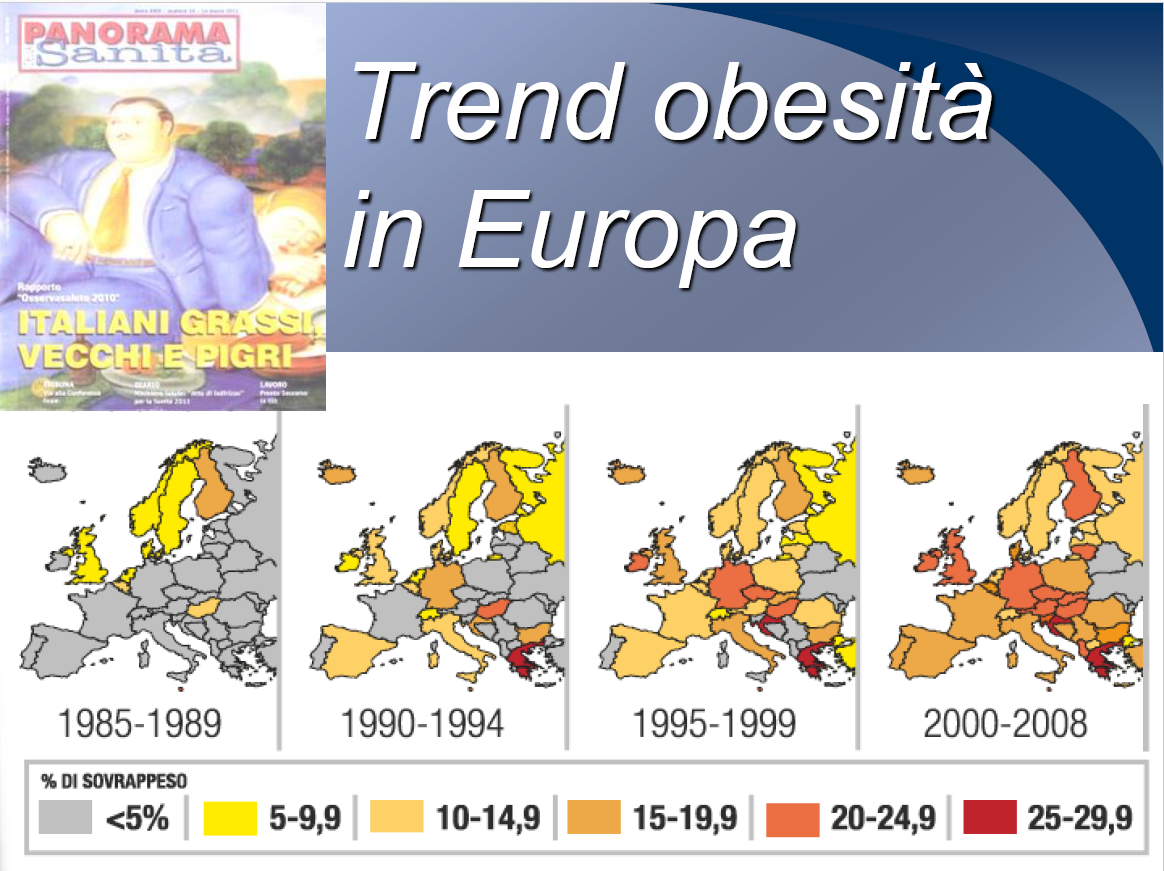
\includegraphics[width=0.7\textwidth]{03/image8.png}
\end{figure}

C'è un'immagine interessante che descrive gli Italiani come vecchi,
grassi e pigri. Se ci chiediamo quanti Italiani svolgono attività
motoria o sportiva, troviamo dei dati che imbarazzano. Meno del 50\%
degli italiani svolge attività motoria o sportiva, il che vuol dire che
abbiamo un popolo sedentario. Il problema riguarda anche i bambini e
questo è un fatto più pericoloso. Infatti il tessuto adiposo si sviluppa
in certi momenti della vita e quindi l'obesità iperplastica porta un
bambino grasso a diventare potenzialmente un adulto grasso. Un soggetto
con elevato numero di cellule adipose se le tiene come corredo della
malnutrizione dell'infanzia e della preadolescenza. Se si guardano i
bambini d'estate si nota subito come un gran numero sia in sovrappeso,
se non addirittura obeso. Si può dire che abbiano un elevato BMI
(parametro che incrocia l'altezza e il peso e determina la situazione di
normopeso, sovrappeso e obeso). C'è uno studio che dimostra che i
proprietari di cani ammalano meno di infarto o di malattie
cardiovascolari, perchè questi, bello o brutto che ci sia, devono farsi
qualche centinaio di metri al giorno per portare fuori l'animale. Queste
persone sono obbligate a farsi almeno un km al giorno. Ovviamente,
sapendo che il bilancio calorico è fatto da entrate e uscite, mangiando
di più (per un fatto culturale e sociale), l'attività motoria dovrebbe
essere adeguata. C'è dunque il problema di iperalimentazione ma anche di
attività motoria scarsa.

\begin{figure}[!ht]
\centering
	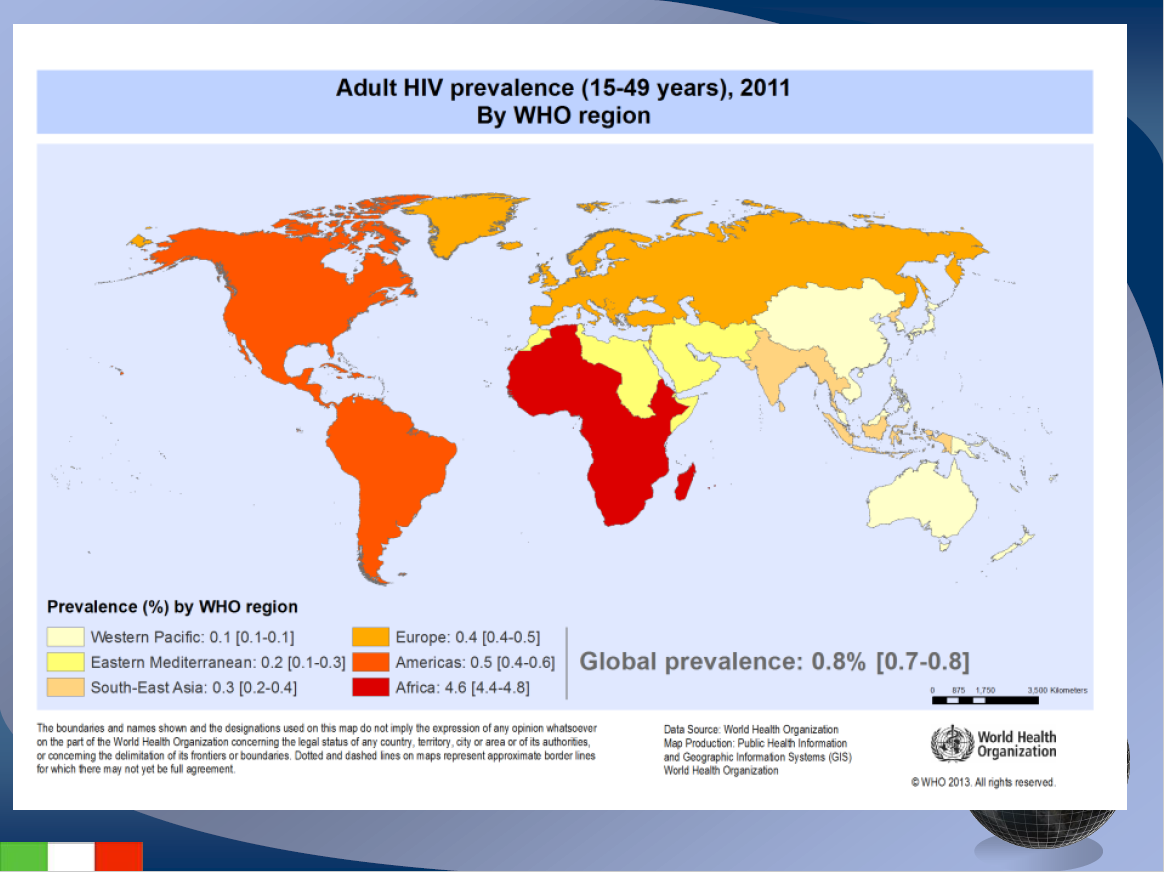
\includegraphics[width=0.7\textwidth]{03/image9.png}
\end{figure}

Prendiamo un altro esempio di prevalenza come quello dell' infezione da
HIV negli adulti, popolazione dai 15 ai 49 anni. Questa è una bella
fotografia che ci dice che oggi, la prevalenza di soggetti HIV nel mondo
è 0.8\%. Ma non è uguale dappertutto. In Europa è 0.4\%, nelle Americhe
0.5\%, in Africa 4.6\%. Alcuni paesi come Australia, Nuova Zelanda,
Giappone e Cina sono allo 0.1\%.

Ci sono poi i big killers che a livello mondiale fanno più morti e per
cui non esistono i vaccini: HIV, TBC e MALARIA. Un milione di morti o
poco meno la malaria e più o meno uguale le altre due patologie. Questi
sono dati di prevalenza, ma se andiamo a vedere l'incidenza, soprattutto
per categoria, scopriamo quali sono i principali fattori di rischio e le
principali categorie, in modo da contenere le patologie. Ad es. in
Africa i modi con cui si trasmette HIV sono 2 ancora: rapporti sessuali
non protetti e trasfusioni di sangue non controllato.

\begin{figure}[!ht]
\centering
	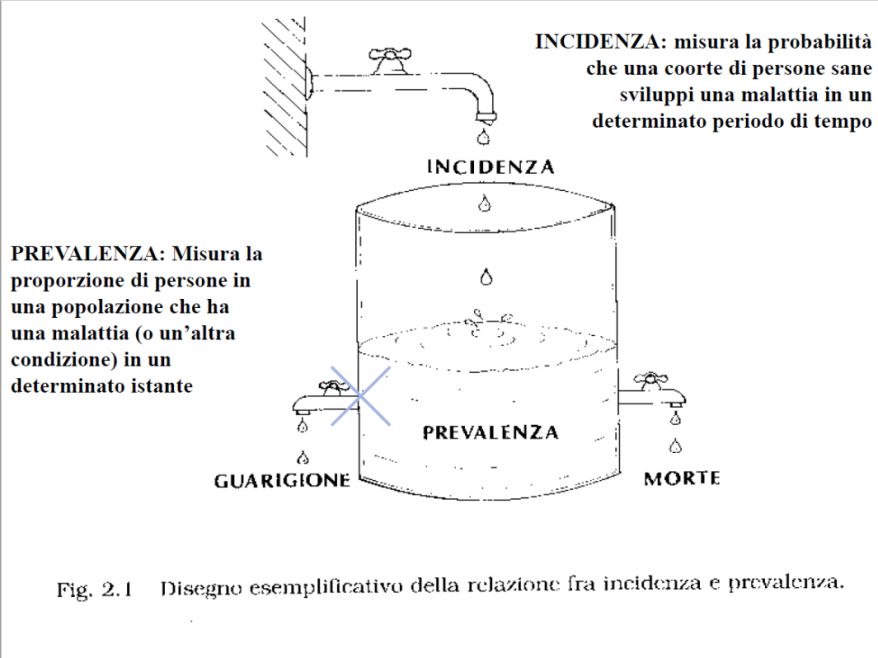
\includegraphics[width=0.7\textwidth]{03/image10.png}
\end{figure}

La botte è stata messa non per capire la differenza
incidenza-prevalenza, ma per comprendere un altro fenomeno. Quando siamo
davanti a dati epidemiologici, dobbiamo porci un problema: come si cessa
di essere un caso di malattia? o si guarisce o si muore. Per assurdo, se
ci fosse una malattia con letalità del 100\% in tempi rapidi, avrei
incidenza quello che è, ma prevalenza 0, quindi una persona appena
ammalata morirebbe (caso limite la rabbia). La rabbia non è curabile, ma
è prevenibile. Addirittura per la rabbia si può fare un vaccino post
esposizione, perchè ha un periodo di incubazione molto lungo. La rabbia
è un problema di sanità pubblica da trattare, ma oggi non dovremmo più
avere morti di rabbia. In realtà ne abbiamo pochi e solo nei paesi in
cui non si fa profilassi post esposizione. Date queste premesse, la
prevalenza della rabbia è zero, perchè come ci si ammala si muore.
Prendiamo il diabete e facciamo conto che la sua incidenza negli ultimi
30 anni non sia cambiata, anche se in realtà non è proprio così. L'acqua
che entra nella botte è sempre quella, il rubinetto della guarigione nel
diabete non c'è perchè chi lo ha se lo tiene per sempre, la letalità è
calata negli anni perchè noi, da vent'anni a questa parte, il diabetico
lo riusciamo a curare molto bene dandogli insulina. La qualità della
vita cala un po', ma il paziente riesce a sopravvivere a lungo. Cosa mi
aspetto dalla botte se riesco a stringere il rubinetto della mortalità
ed è chiuso quello della guarigione? A parità di incidenza mi aspetto
che aumenti la prevalenza. L'incidenza stabile con la prevalenza in
aumento non è negativo come dato. Questo dato ci dice che si muore meno,
quindi curo meglio il diabete. Se voglio monitorare nel tempo
l'andamento di una malattia, calcolo l'incidenza. Ma la prevalenza mi
serve per capire quanti casi sono e quindi prevedere la preparazione di
ambulatori, farmaci e personale sanitario adeguato.

\subsubsection{Misure epidemiologiche descrittive}


\begin{figure}[!ht]
\centering
	
\includegraphics[width=0.7\textwidth]{03/image11.png}
\end{figure}

La mortalità è un'incidenza in cui l'evento è la morte della
popolazione. La natalità è sempre un tasso di nati vivi rispetto ai
residenti in quel periodo. Il tasso di natalità in Italia all'ultimo
censimento del 2011 è 9.1 x 1000, la mortalità 9.7 x 1000. In Italia in
questo momento muoiono più persone di quante ne nascono, però la
popolazione è sempre di 60.000.000 e questo grazie all'immigrazione.

\begin{figure}[!ht]
\centering
	
\includegraphics[width=0.7\textwidth]{03/image12.png}
\end{figure}

Se poi andiamo a misurare i tassi di fecondità (numero di nati vivi in
rapporto alle donne in età fertile), l'Italia è a percentuali dell'1.2,
con \% sotto l'1 per gli italiani e superiori per gli stranieri. La
fecondità nazionale continua ad essere concretamente sostenuta dalle
donne straniere con 2.07 figli rispetto alle Italiane con 1.33.

L'ultimo gruppo di misure descrittive sono rappresentate in questa
immagine:

\begin{figure}[!ht]
\centering
	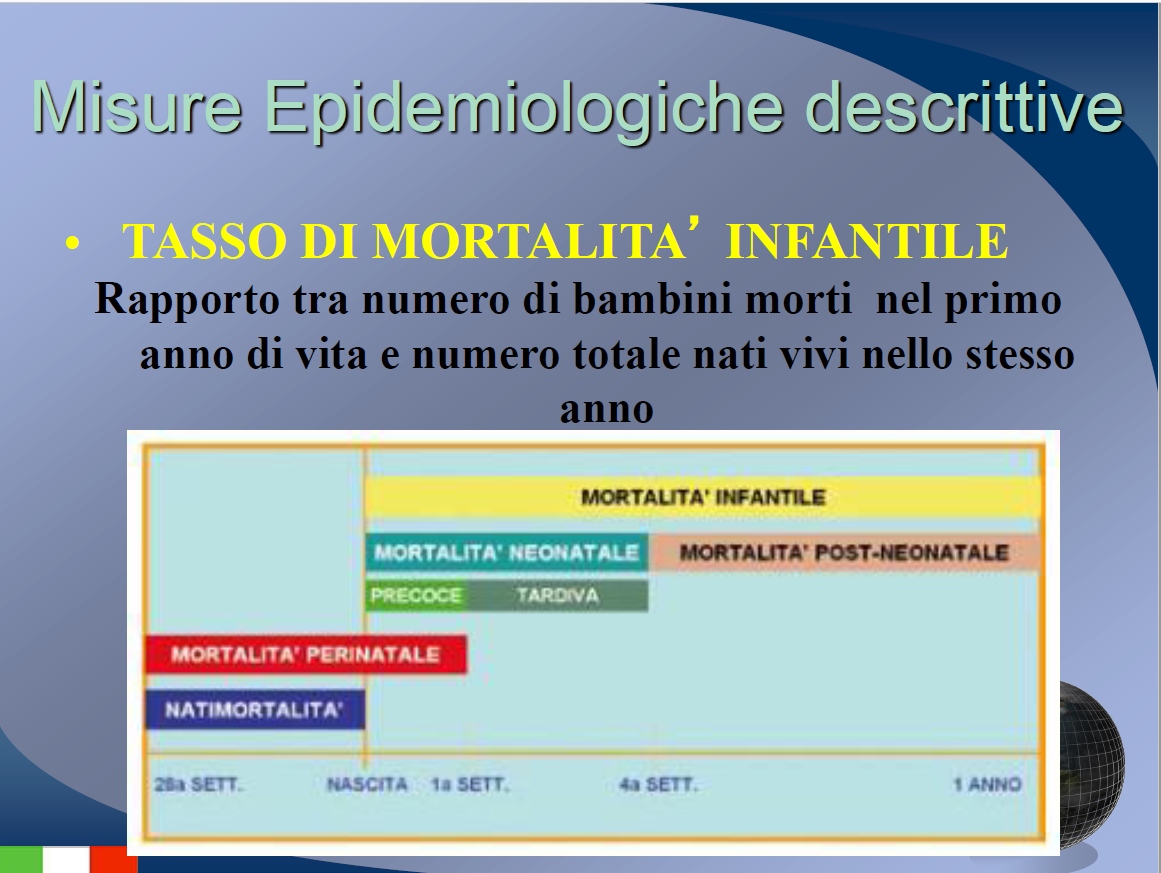
\includegraphics[width=0.7\textwidth]{03/image13.png}
\end{figure}

Ci sono alcune situazioni in cui il dato epidemiologico mi serve per
indagare alcuni fenomeni. Se prendo la \textbf{mortalità perinatale},
questa prende in considerazione le morti fetali più le morti nella prima
settimana di vita. La \textbf{nati-mortalità} tutte le morti fetali. La
\textbf{mortalità infantile}, i morti nel primo anno di vita, che a sua
volta può essere scorporata in \textbf{mortalità neonatale} nel 1\^{}
mese e \textbf{post neonatale} dal 2\^{} al 12\^{} mese. La stessa
mortalità neonatale si divide in \textbf{PRECOCE} nella 1\^{} settimana
e \textbf{TARDIVA} dalla 2\^{} alla 4\^{} settimana di vita. Tutti
questi tassi sono importanti per capire la mortalità e in più essendo
specifici per alcune categorie ci dicono diverse cose. La mortalità
infantile ad esempio è un indicatore molto preciso della situazione
igienico-sanitaria dell'area per cui noi calcoliamo il tasso. In Italia
è il 5 X 1000, in Africa il 40 X 1000. La mortalità perinatale che
analizza l'ultimo periodo di gravidanza e la prima settimana di vita, è
un indicatore dell'assistenza al parto ed alla gravidanza. Se trovo una
mortalità perinatale alta, significa che c'è qualcosa che non funziona
nell'assistenza al parto stesso. In questo caso muoiono per
malformazioni fetali, nella mortalità infantile si muore per malattie
infettive. La causa più comune di mortalità infantile in Italia è la
SIDS o comunemente detta morte in culla. Abbiamo talmente ridotto tutte
le cause di morte per altre ragioni, che è rimasto un 1,5 x 1000 su 5
legato a questa SIDS di cui in realtà non si conosce bene l'origine.
Sono arresti cardiaci improvvisi ed inaspettati.

\subsection{Misure di effetto}


\begin{figure}[!ht]
\centering
	
\includegraphics[width=0.7\textwidth]{03/image14.png}
\end{figure}

Veniamo ora alle \textbf{MISURE DI EFFETTO}: \emph{misurano il ruolo che
possono avere le esposizioni}.

Genericamente, sono confronti tra frequenze di malattie in gruppi
diversi. Abbiamo visto prima che ci sono le esposizioni. Se vogliamo
valutare il ruolo di un esposizione e se questa è collegata o no ad una
malattia, dobbiamo avere un secondo gruppo per calcolare la stessa
misura, l'incidenza, in chi non è esposto. Quindi se voglio calcolare il
rischio di tumore nei fumatori rispetto ai non fumatori, calcolerò
l'incidenza nel primo e nel secondo gruppo, per poter arrivare ad una
misura che si chiama \textbf{RISCHIO RELATIVO}.

\begin{figure}[!ht]
\centering
	
\includegraphics[width=0.7\textwidth]{03/image15.png}
\end{figure}

Il rischio relativo è l'incidenza negli esposti, diviso l'incidenza nei
non esposti. Si chiama r1/r0. Se gli esposti hanno la stessa incidenza
dei non esposti, il risultato sarà 1. Non verrà mai l'1 preciso perchè
c'è la fluttuazione statistica. Mi aspetto un numero vicino a 1 e
comunque, con le tecniche statistiche dei limiti di confidenza che
includono l'1, e che ci fanno capire come ci può essere una
fluttuazione, ma comunque stiamo intorno al'1, che significa nessun
effetto. Quando ho un rischio relativo superiore a 1, il 7 del fumo ad
esempio, cosa significa? Che i fumatori hanno un rischio di ammalare di
tumore superiore di 7 volte ai non fumatori. Ci sono anche i tumori al
polmone non associati al fumo, ma chi fuma ha un rischio maggiore, anche
in proporzione alla quantità di sigarette fumate. Il fumo da effetti a
lungo termine. il tempo di latenza per un effetto grave nel fumatore è
di 15-20 anni. Chi fuma a 20 anni non ha l'evento sanitario a 25, ce
l'ha a 45. L'epidemiologia attraverso studi sofisticati ci ha detto
un'altra cosa. L'ex fumatore non va a zero come rischio subito, ma va a
zero dopo 15 anni. Se il fumatore di adesso (23 anni) smette, a 40 anni
torna al rischio dei non fumatori. Il benefit è che il fumatore di 20
anni rischia 7 volte in più, ma 7 volte in più di una quota bassissima.
Dallo 0.1 x 100.000 diventa 0,7 x 100.000. I tumori al polmone a 20 anni
sono rarissimi e quindi c'è un maggior rischio relativo, ma un valore
insignificante in termini di rischio reale. A 40 anni le cose iniziano a
cambiare. Questo per dire che se l'abitudine viene dismessa presto,
probabilmente in termini assoluti, il rischio aggiuntivo del fumo a 20
anni è molto limitato. Molto diverso è quando il rischio si attesta a
1.1. C'è una controversia epidemiologica sulla pillola e l'aumento del
rischio del tumore al seno. Quando arriva uno studio che prova che il
rischio relativo di 1.1 è reale, in commercio c'è già una pillola con
dosaggi minori e quindi si dice che quello è il risultato della pillola
di vecchia generazione. Qualche volta abbiamo a che fare con risultati
\textless{}1. In questo caso non abbiamo a che fare con fattori di
rischio, ma l'esposizione è protettiva. Se inserisco il numero di
chilometri percorsi al giorno ed il rischio cardiovascolare, mi verrà un
risultato negativo e cioè camminare è un fattore protettivo e non un
fattore di rischio. Un esempio clamoroso: rischio relativo di 31
-\/-\/-\textgreater{} soggetti affetti da HIV hanno 31 volte più
probabilità di ammalare di polmonite di soggetti sani. E' chiaro il
perchè: HIV immunodeprime e ciò favorisce lo sviluppo di patologie
infettive. In uno studio condotto in Portogallo, il rischio di basso
peso alla nascita è 2 volte maggiore nelle famiglie a basso reddito
rispetto a quelle ad alto reddito. Il rischio relativo è 2. Poi il
fenomeno è da studiare nella sua interezza, valutando se ci sono fattori
di confondimento, perchè non è detto che il rischio relativo fornisca il
risultato (come mai pesano meno questi neonati? vengono nutriti meno?
peggio?...).

\begin{figure}[!ht]
\centering
	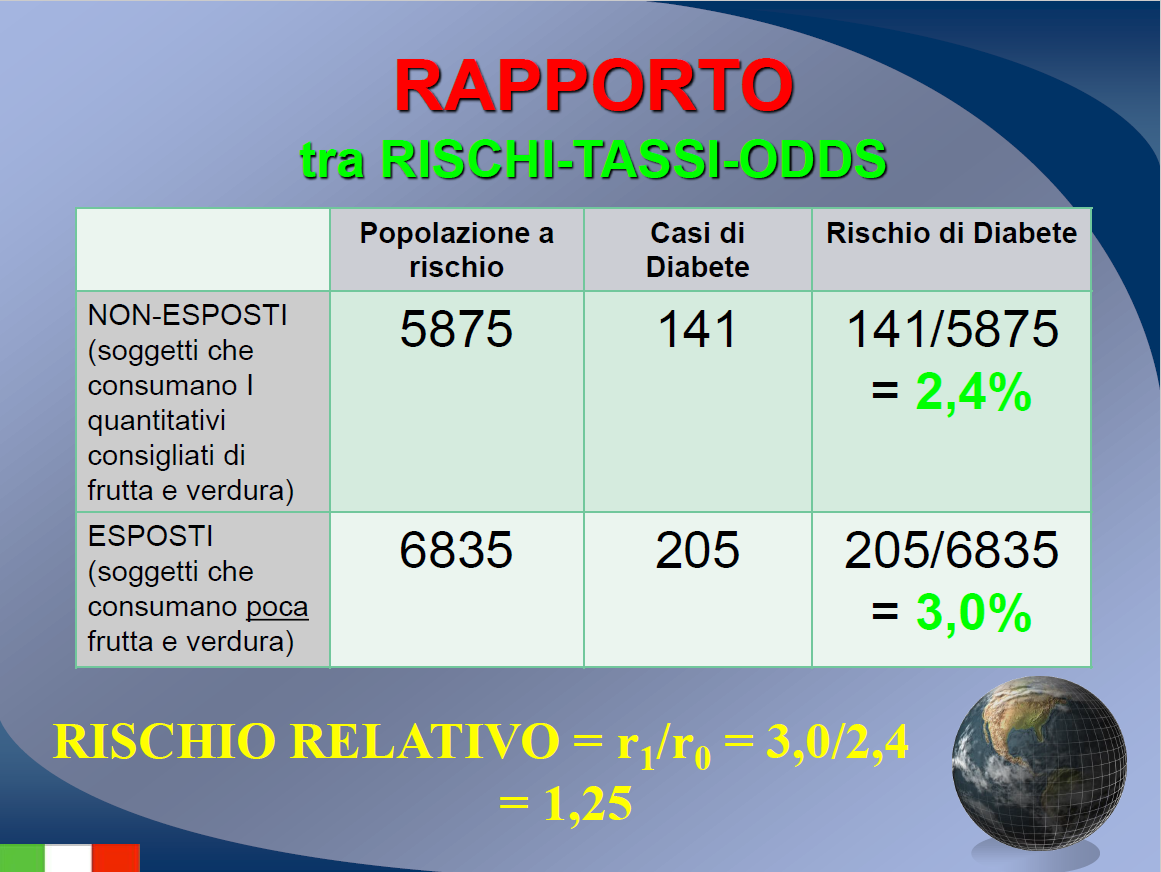
\includegraphics[width=0.7\textwidth]{03/image16.png}
\end{figure}

Guardiamo ora la popolazione a rischio per i casi di diabete. I non
esposti sono i soggetti che consumano adeguati quantitativi di frutta e
verdura, gli esposti quelli che non lo fanno. La differenza c'è, anche
se non macroscopica. Questo ci permette di individuare la frutta e la
verdura come fattori protettivi o la loro assenza come fattori di
rischio. Il rischio relativo è di 1.25. Per tutti questi rischi bisogna
poi calcolare i limiti di confidenza, questione che attiene alla
statistica. Tanto più ampio è il campione, quanto più le fluttuazioni
saranno minori. Su 10 casi le fluttuazioni saranno più ampie perchè ci
possono essere 20 casuali che influenzano i dati.

Fin qui abbiamo parlato di associazioni statistiche che indirizzano
verso una certa ipotesi, la quale è però da confermare, perchè ci
possono essere due generi di interferenze esterne: quelli che vengono
chiamati \textbf{BIAS} e \textbf{FATTORI DI CONFONDIMENTO}.
\\\\
• Il bias è una \emph{distorsione} perchè a volte sono errori di
rilevamento, a volte di conduzione dello studio, altre volte contingenti
legati al tipo di studio. Ad es. quando facciamo uno studio
caso-controllo e cerchiamo i fattori di rischio delle malformazioni
congenite nelle donne che partoriscono bambini malformati rispetto a
donne che partoriscono bambini sani e andiamo a fare l'anamnesi, la
categoria delle donne che hanno partorito un bambino malformato,
ricordano tutto quello che hanno fatto in gravidanza, mentre le altre
ricordano molto meno. Qui noi allora possiamo avere quello che in gergo
tecnico è chiamato \textbf{RECALL BIAS}. Questo non è un errore, ma è
una situazione per cui nel rilievo vedo che un gruppo di soggetti
ricorda meglio. Quando farò l'analisi dei risultati, quel gruppo
risulterà aver riferito un certo elemento che è classificato fattore di
rischio, ma che in realtà magari non lo è, perchè nell'altro gruppo c'è
una sottostima nella raccolta del dato. Questo è il motivo per cui li
chiamiamo bias e non errori.
\\\\
• Il fattore di confondimento è un altro elemento importante. Se valuto
l'andamento di un tumore nei lavoratori di un'azienda rispetto alla
popolazione generale e nell'azienda la prevalenza dei fumatori è doppia
rispetto alla popolazione generale, trovo sicuramente un rischio
relativo significativamente maggiore a uno e quello non è
necessariamente legato all'azienda, ma magari solo al fatto che lì ci
sono abitudini individuali diverse. Il ruolo del fumo in questo caso è
un fattore esterno che influenza l'interpretazione, è un fattore di
confondimento. Se quando studio i lavoratori di un azienda, calcolo
anche la prevalenza del fumo nella stessa rispetto alla popolazione
generale, il confondimento in fase di analisi dei dati lo posso
eliminare.

Dopo aver definito la presenza di bias, come facciamo a capire se
l'associazione è causale o no? Cioè se effettivamente abbiamo a che fare
con un'esposizione che aumenta la probabilità? Dobbiamo andare per
deduzione, vedere se c'è un rapporto temporale tra esposizione ed
effetto, se c'è plausibilità biologica (attenti perchè a volte i
meccanismi non li conosco), la consistenza dei diversi studi (se più
studi portano allo stesso risultato).

Riassumendo: il rischio relativo ci da la misura dell'associazione;
questa associazione per poter essere ipotizzata come causale richiede un
processo che non è statistico, ma è logico. Questo è il motivo per cui
l'epidemiologia è molto legata alla medicina. Non basta la statistica
pura.



\section{Disegni di Studio}

\subsection{La ricerca scientifica}


Il primario interesse dei medici è il beneficio del pz e della comunità.
Come ci si arriva? È un processo lungo, che parte dalla ricerca
scientifica. Con questa si fa un ``focus on the bigger picture'', ovvero
si cerca di mettere in un contesto ciò che stiamo cercando con una
prospettiva più macroscopica. Per mezzo di questo di arriva al beneficio
del pz, questo processo è come la ricerca scientifica e nello specifico
la ricerca epidemiologica supporta il beneficio del pz nella clinica di
tutti i giorni.
\begin{figure}[!ht]
\centering
	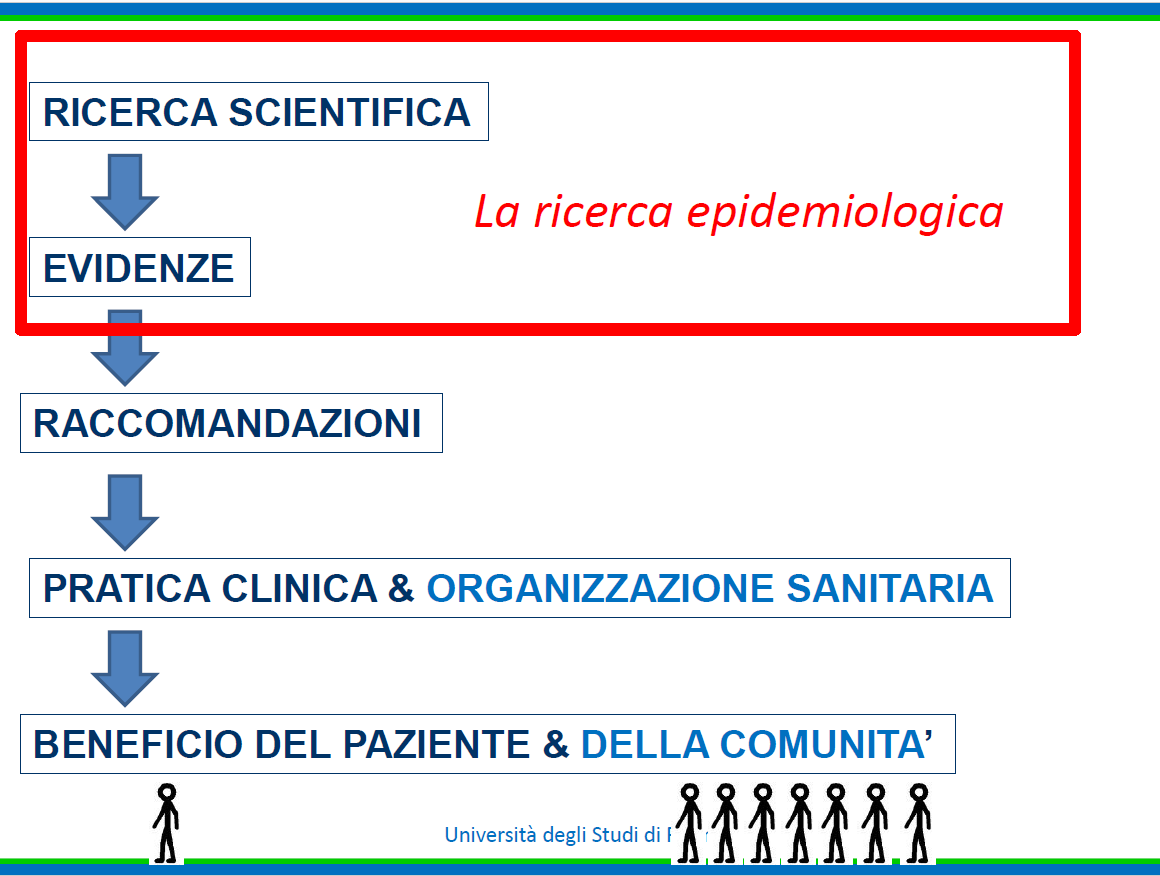
\includegraphics[width=0.8\textwidth]{04/image1.png}
	\end{figure}




\emph{Ricerca scientifica focus on the bigger picture beneficio del pz}

Vedremo quindi quali sono gli step di questo processo.

Ci sono ricerche scientifiche di vari tipi, qui ci si concentra sulla
ricerca epidemiologica.

\subsubsection{La ricerca epidemiologica}

La ricerca scientifica permette di arrivare ad \textbf{evidenze}, quindi
tesi supportate da ricerche dati su popolazioni.

Le evidenze vengono utilizzate per produrre \textbf{raccomandazioni},
come le linee guida.

Dalle linee guida si può fare pratica clinica ed organizzazione
sanitaria basata sulle evidenze e si raggiunge il fine ultimo, che è il
\textbf{beneficio} \textbf{del pz e delle popolazioni.}

\emph{Ricerca scientifica evidenze raccomandazioni buona pratica clinica
beneficio pz e popolazioni}

Nell'ambito della ricerca biomedica ci sono 4 livelli:

\begin{itemize}
\item
  dimensione molecolare (biologia, immunologia)
\item
  dimensione dei tessuti e degli organi (istologia, anatomia patologica,
  quindi indagini di laboratorio sui tessuti)
\item
  dimensione dell'individuo (pratica clinica)
\item
  dimensione della popolazione (epidemiologia): questa è quella su cui
  ci si focalizza qui.
\end{itemize}

\paragraph{Epidemiologia }


L'epidemiologia si occupa della raccolta e analisi di \emph{dati di
popolazione} con un fine che può essere

\begin{itemize}
\item
  DESCRITTIVO: descrivere la distribuzione dei fenomeni sanitari (es.
  prevalenza a livello mondiale della malaria)
\item
  ANALITICO: indagare i determinanti delle malattie (il termine
  ``cause'' al posto di ``determinanti'' è un po' impreciso, ma può
  servire per ricordare il concetto)
\end{itemize}

Si delineano diversi stadi:

\begin{enumerate}
\def\labelenumi{\arabic{enumi}.}
\item
  Study design, ovvero il disegno, la progettazione dello studio
  epidemiologico
\item
  Raccolta dei dati
\item
  Analisi dei dati
\item
  Interpretazione dei dati
\end{enumerate}

{[}nel programma di epidemiologia sono previsti 4 argomenti: fonti dati,
disegni di studio, analisi dati, interpretazione dati{]}

\paragraph{Disegni di studio}


L'epidemiologia raccoglie dati di popolazione, come questi dati vengono
raccolti e organizzati è il disegno di studio.

Ad esempio si può fare un disegno di studio per dimostrare
l'associazione tra fumo di sigaretta e neoplasia polmonare. Sembra
banale, ma è stato dimostrato con studi epidemiologici. Il disegno
organizza i dati al fine di rispondere a determinati quesiti di ricerca,
in questo caso la correlazione fumo-tumore al polmone.

Caratteristiche dei disegni di studio:

\begin{itemize}
\item
  dipendono dal quesito di ricerca (obiettivo) dello studio
\item
  sono influenzati dalla \emph{fattibilità}

  \begin{itemize}
  \item
    disponibilità di risorse economiche
  \item
    aspetti etici
  \item
    tempo
  \end{itemize}
\item
  determinano l'analisi statistica
\end{itemize}

Perché è importante conoscere i diversi disegni di studio?

\textbf{1.} Pianificare il progetto di ricerca, ad esempio per chiedere
fondi o fare una tesi. La conoscenza dei diversi tipi di disegni di
studio vi permette di selezionare le popolazioni oggetto di studio, di
definire gli outcome di interesse, di raccogliere i dati che sono
necessari e pianificare il tipo di analisi.

\textbf{2.} Per individuare i limiti legati a ciascun disegno di studio,
che ne condizionano la solidità delle evidenze prodotte.

Questa è la piramide delle evidenze:

\begin{figure}[!ht]
\centering
	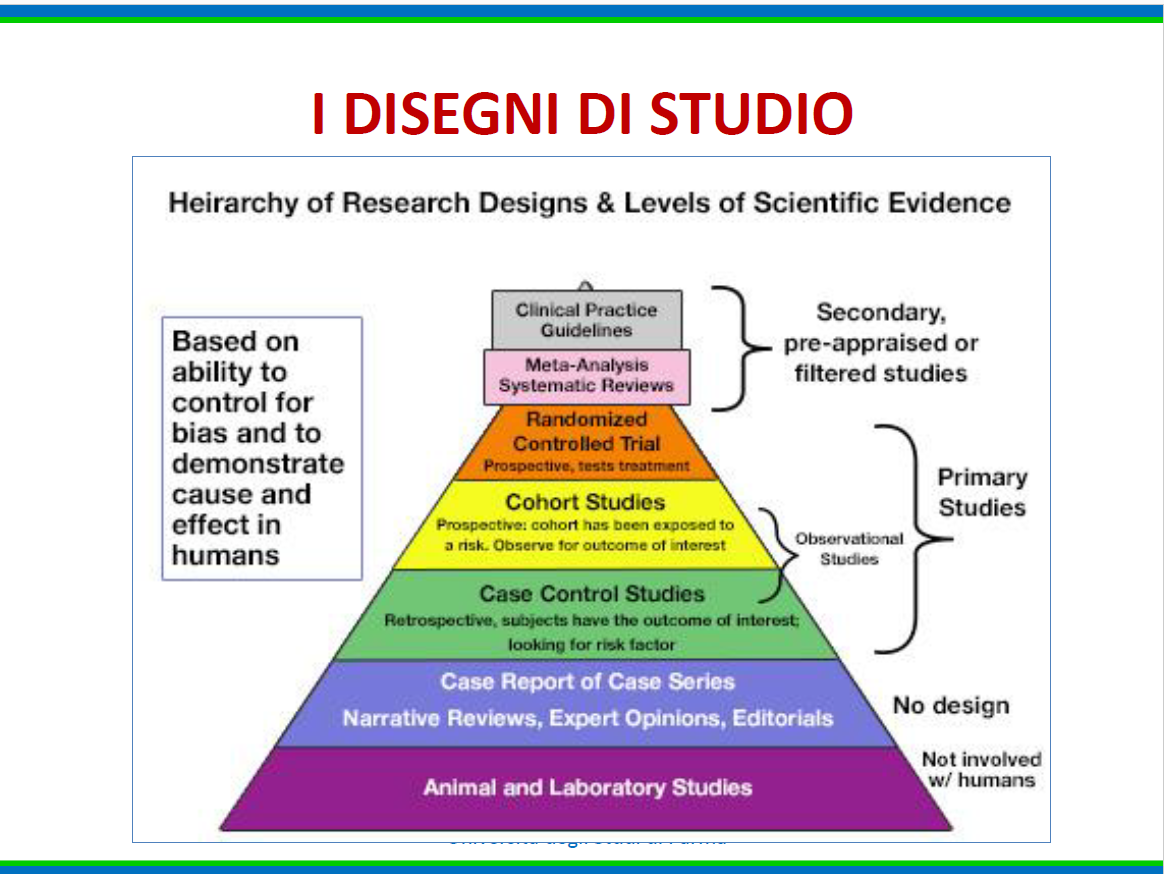
\includegraphics[width=0.8\textwidth]{04/image2.png}
	\end{figure}

Essa suddivide i disegni di studio in base al grado di solidità delle
evidenze, alla base ci sono gli studi più deboli e all'apice quelli più
solidi (meno limitate da bias ecc).

\subparagraph{Classificazione dei disegni di studio}


Ci sono diverse classificazioni, ma tutte li dividono su 3 livelli:

\begin{itemize}
\item
  \emph{fine}: descrittivo o analitico
\item
  \emph{dati}: aggregati o disaggregati
\item
  \emph{disegno}: osservazionali o sperimentali
\end{itemize}

dati

\emph{disaggregati}: di singoli individui

\emph{aggregati}: di gruppi di individui (ad esempio incidenza tumore
alla mammella in Emilia Romagna vs Toscana, confronta gruppi di
individui)

disegno (la più classica)

- \emph{osservazionali}: osservare i fenomeni e basta

- \emph{sperimentali}: viene introdotto ai fini della ricerca
l'esposizione, la terapia o l'intervento.

I più classici degli sperimentali sono i trials clinici, soprattutto
quelli che valutano l'efficacia dei farmaci.

\begin{figure}[!ht]
\centering
	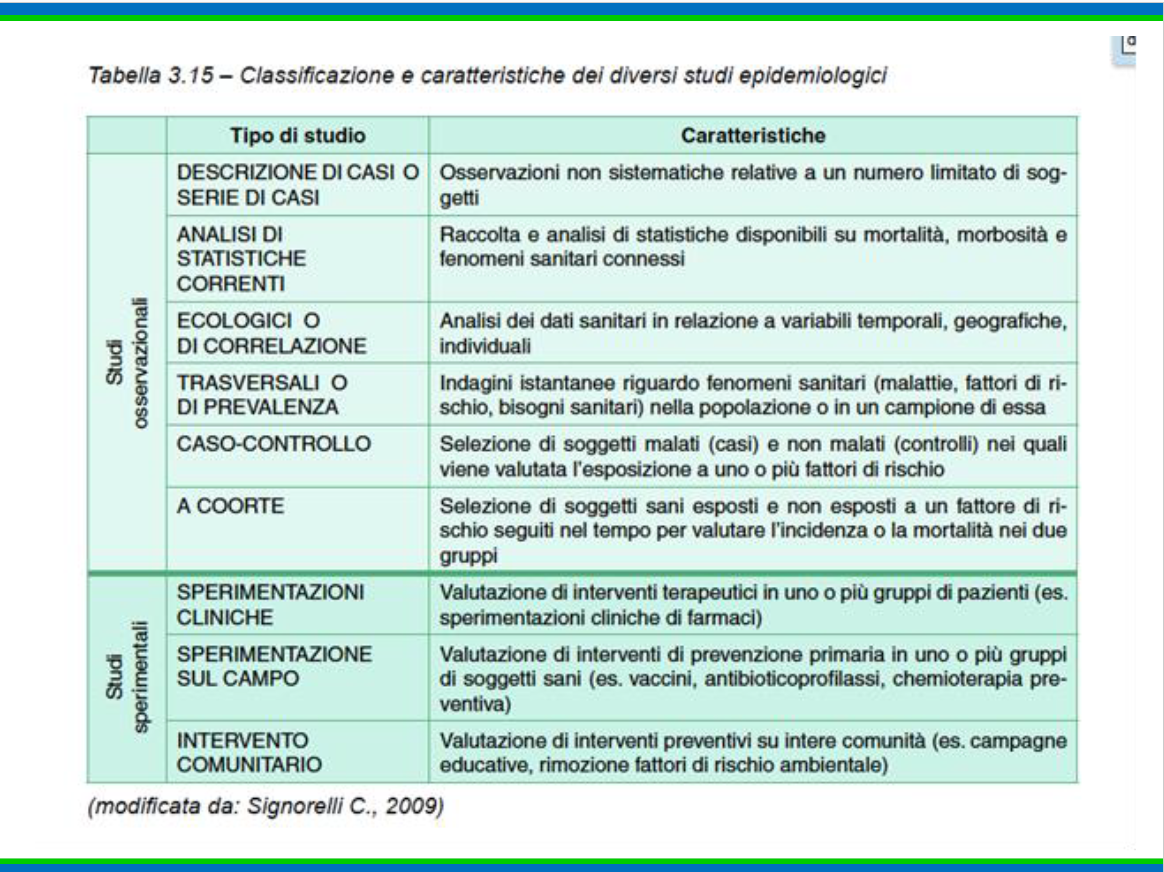
\includegraphics[width=0.8\textwidth]{04/image3.png}
	\end{figure}

\subparagraph{Studi osservazionali }


A) \textbf{Case report} (descrizione di casi clinici) e \textbf{Case
series} (serie di casi): osservazioni non sistematiche relative a un
numero limitato di soggetti.

\begin{enumerate}
\def\labelenumi{\arabic{enumi}.}
\item
  \textbf{Case report}: descrizione dettagliata di segni e sintomi e
  risultati di laboratorio di un caso singolo.
\end{enumerate}

Perché è utile? Potrebbe essere un caso particolarmente interessante che
può stimolare la riflessione. Di solito vengono pubblicati casi
eclatanti o particolarmente importanti.

\begin{enumerate}
\def\labelenumi{\arabic{enumi}.}
\item
  \textbf{Case series}: descrizione dettagliata di segni e sintomi e
  risultati di laboratorio di un numero limitato di casi (fino a 5
  casi).
\end{enumerate}

B) \textbf{Analisi di statistiche correnti}: studi descrittivi che usano
\emph{dati aggregati}, dati amministrativi, statistiche ricorrenti;
descrivono eventi sanitari per età, sesso, periodo, distribuzione
geografica.

Es. Incidenza di tubercolosi nel mondo. Dalla figura si vede come sia
maggiore in Sud Africa (blu scuro) rispetto Nord America ed Europa
(azzurro). A cosa ci può servire questo dato? Può essere utile a livello
politico sanitario per allocare risorse e per la programmazione di
interventi sanitari, quindi incide sull'organizzazione della sanità
pubblica.

\begin{figure}[!ht]
\centering
	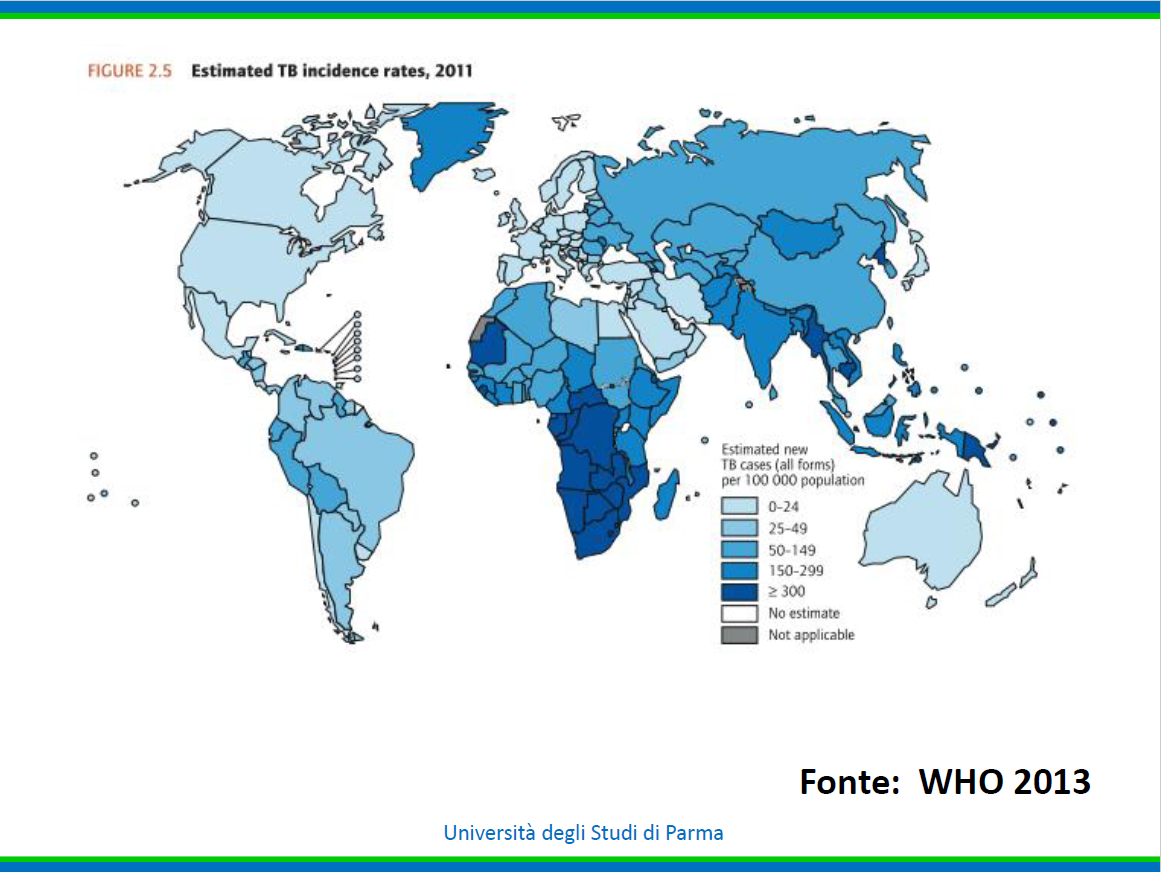
\includegraphics[width=0.8\textwidth]{04/image4.png}
	\end{figure}

C) \textbf{Studi ecologici o di correlazione}: utilizzano \emph{dati
aggregati} non solo per descrivere un fenomeno, ma anche per studiarne i
determinanti. Anche questi utilizzano dati provenienti da flussi
amministrativi e statistiche correnti.

Vengono fatti perché generalmente poco costosi e relativamente rapidi,
proprio perché utilizzano dati già disponibili, anche se hanno una serie
di limitazioni.

Riassumendo, studia l'associazione tra un'esposizione e un outcome,
utilizzando dati aggregati.

\emph{Ciò che fa sempre uno studio è studiare questa associazione tra
un'esposizione, ovvero un fattore di rischio, e un outcome, ovvero una
malattia.}

Es. studio pubblicato sul BMJ del 2014: ha come indicatori sanitari 170
paesi per tipo di economia e grado di democrazia.

\begin{figure}[!ht]
\centering
	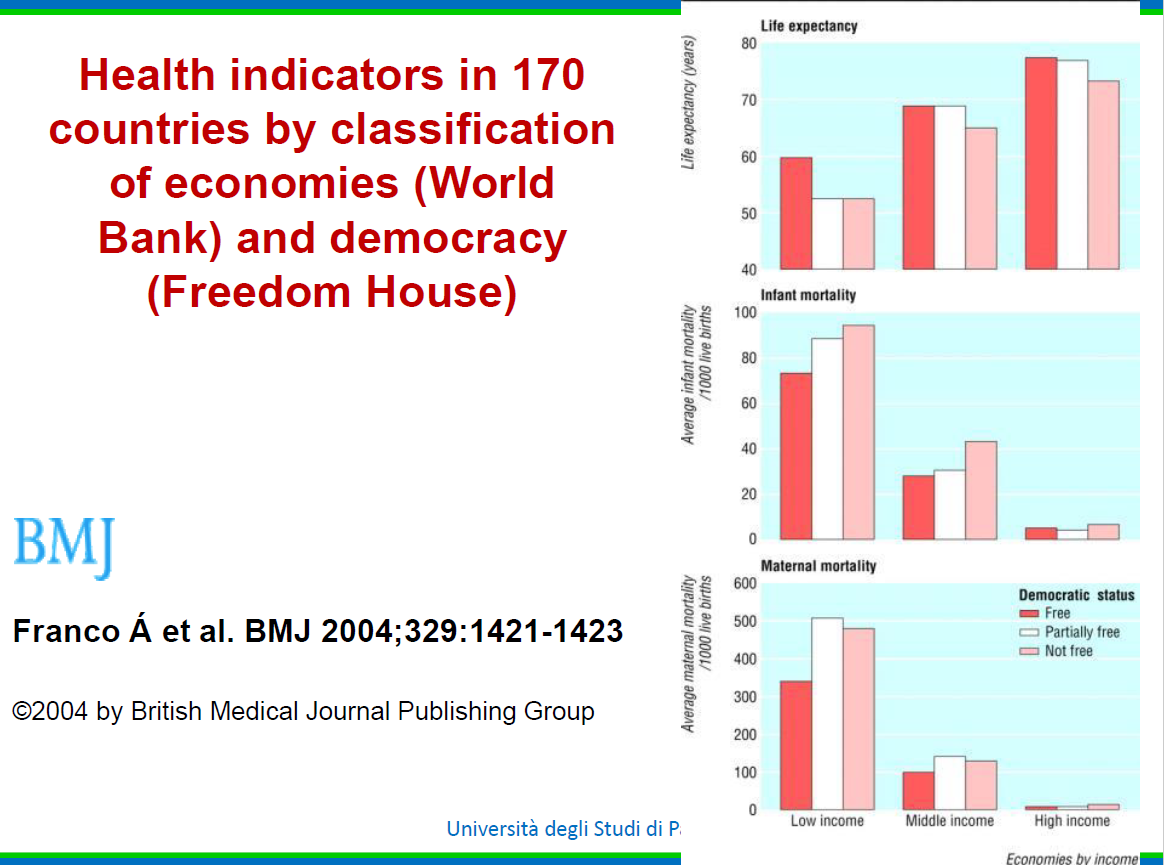
\includegraphics[width=0.8\textwidth]{04/image5.png}
	\end{figure}

Ci sono tre outcome: aspettativa di vita (grafico in alto), la mortalità
infantile (grafico in mezzo) e la mortalità materna (grafico in basso).

Esposizione: stato socioeconomico e livello di democrazia.

Il quesito di ricerca di partenza è: paesi con stato socio economico
diverso, hanno diversi outcomes sanitari?

Sono stati classificati 170 paesi con diverso gradi di esposizione (sono
dati aggregati, di interi paesi): poveri (gruppo di colonne a sinistra
di ciascuna delle tre tabelle), medi (colonne centrali), ricchi (a
destra).

Nel primo ad esempio l'aspettativa di vita aumenta in base allo stato
economico, è minore nei Paesi più poveri. Questa è la risposta al primo
quesito.

Poi i ricercatori hanno posto un secondo quesito: lo stato democratico
influenza questo outcome?

(stato democratico libero: colonne rosse; parzialmente libero: colonne
bianche; non libero: colonne rosa).

La mortalità infantile ad esempio per tutti i gradi di ricchezza è più
alta nei non democratici.

Quindi questo è un esempio di come dati aggregati di nazioni possano
essere usati per studiare l'associazione tra un' esposizione e un
outcome di interesse.

D) \textbf{Studi trasversali o di prevalenza}, cosiddetti \emph{studi
cross-sectional} (l'esempio più classico sono i questionari).

L'informazione è raccolta

\begin{enumerate}
\def\labelenumi{\arabic{enumi}.}
\item
  in un istante temporale definito, a un tempo 0 (es. numero di fumatori
  degli studenti di medicina anno 2016-2017), è uno studio
  \emph{trasversale}
\item
  dati da \emph{singoli individui}
\item
  dati su esposizione e/o outcomes (es. quesito ``vivere in un'area
  inquinata favorisce l'allergia?'': dove vive il soggetto=esposizione;
  è allergico=outcome)
\end{enumerate}

Gli studi trasversali sono tanto più validi e solidi, quanto più vengono
fatti su un campione che viene definito \emph{rappresentativo.}

Es. quesito: prevalenza del fumo nei ragazzi italiani di 23 anni. Per
avere la verità più assoluta si dovrebbero mandare questionari, lettere
via email a tutti i ragazzi italiani, ma questo per questioni di
fattibilità non è possibile (troppo dispendioso, troppo tempo ecc). Si
fa allora un \textbf{campione rappresentativo}: ci sono tecniche di
campionamento che mi permettono di selezionare un campione
rappresentativo.

Nella selezione è importante il concetto ``rappresentativo'': non si può
fare ad esempio solo sugli universitari, perché si avrebbero differenze
con i ragazzi lavoratori per abitudini. Se si fa solo sugli universitari
ovviamente poi si deve interpretare il dato considerando che non
riguarda tutti i ragazzi italiani: sarà rappresentativo della sola
popolazione universitaria.

La solidità dello studio trasversale è quindi legata alla
rappresentatività del campione che noi selezioniamo.

Es. Il The Lancet ha pubblicato nel 2013 un articolo sulle abitudini
sessuali inglesi, un esempio di studio cross-sectional. Perché ci può
essere un interesse di sanità pubblica? Per il controllo delle malattie
sessualmente trasmesse e l'educazione sessuale legata ai metodi
contraccettivi (in Inghilterra ci sono molte maternità giovanili non
volute).

Altro studio cross-sectional su Jama Neurology: la depressione (outcome)
in associazione alla disfunzione cognitiva (esposizione) misurata con
tecniche di neuroimaging negli ex giocatori di football professionisti.
Hanno comparato giocatori con impairment cognitivo e depressione e
giocatori con livello cognitivo normale e assenza di depressione.

Caratteristiche studi cross-secional:

\begin{itemize}
\item
  esposizione e outcome sono misurati \emph{allo stesso tempo}
\item
  relativamente rapidi ed economici
\end{itemize}

\begin{quote}
Limiti:
\end{quote}

\begin{itemize}
\item
  Reverse causality: siccome misura esposizione e outcome allo stesso
  tempo non permette di stabilire se l'esposizione viene prima o dopo
  l'outcome, non possiamo stabilire se in realtà non sia l'outcome che
  favorisce l'esposizione di interesse
\item
  Rischio di bias (di selezione)
\item
  Confondimento
\end{itemize}

E) \textbf{Studi a coorte} e \textbf{studi caso-controllo}

Entrambi studiano sempre l'associazione tra un'esposizione e un outcome,
ma in un modo diverso.

• Gli \textbf{studi a coorte} sono \emph{prospettici, longitudinali}. Si
studia una popolazione di esposti e una popolazione di non esposti nel
tempo e si valuta l'incidenza di malattia, l'insorgenza di nuovi casi
negli esposti e nei non esposti. Poi si calcola il rischio relativo, che
è il rapporto tra incidenza degli esposti e quella dei non esposti, se
\textgreater{}1 allora l'esposizione è un fattore di rischio.

Es. Si segue una popolazione di fumatori e una di non fumatori per 10
anni e si valuta l'incidenza di tumore polmonare nei due gruppi e quindi
il rischio relativo, se \textgreater{}1 allora il fumo è un fattore di
rischio.

Caratteristiche:

\begin{itemize}
\item
  l'esposizione è misurata \emph{prima} dell'insorgenza dell'outcome
\item
  questo riduce il bias
\item
  sono più costosi, perché si seguono i pz anche per molti anni
\item
  tempi prolungati
\item
  rischio di perdita al follow up, essendo per molto tempo posso perdere
  i pz perché si trasferiscono o comunque non si presentano più ai
  controlli
\end{itemize}

Es. Outcome di neoplasia polmonare in pz con esposizione
all'inquinamento atmosferico.

Studio del The Lancet: ha utilizzato 17 coorti (17 gruppi di cittadini
in 9 paesi europei), che sono stati studiati in modo prospettico per un
periodo medio di follow up di 12,8 anni, esposti a inquinamento
atmosferico. L'analisi ha dimostrato un'associazione statisticamente
significativa tra il rischio di tumore al polmone e un valore di PM
(particulate matter) 10 definito inquinante, con rischio relativo di
1,2.

• Gli \textbf{studi caso-controllo} partono invece dai casi e dai
controlli, ovvero i malati e i non malati e valutano in maniera
retrospettiva l'esposizione. La valutazione va indietro rispetto al
tempo.

Es. considerando sempre l'esempio dei fumatori, non si dividono fumatori
e non fumatori, ma si prendono i soggetti con neoplasia polmonare e
quelli definiti ``di controllo'' sani e si valuta in modo retrospettivo
l'esposizione al fumo di sigaretta. Si arriva alla fine a determinare in
maniera diversa sempre l'associazione tra esposizione e outcome.

Caratteristiche:

\begin{itemize}
\item
  i pz sono selezionati in base all'outcome, non in base all'esposizione
\item
  non c'è rischio di perdita al follow up, perché li prendo già malati o
  non malati e indago retrospettivamente l'esposizione
\item
  relativamente rapidi (non devo aspettare l'insorgenza di malattia) e
  meno costosi
\end{itemize}

però forniscono evidenze meno solide rispetto agli studi a coorte:

\begin{quote}
- rischio bias, il più comune è il bias di informazione (se indago
l'esposizione al fattore di rischio nei due gruppi, malati e non malati,
il ricordo è maggiore nei malati, per cui si ha un errore sistematico
con sovrastima)

- confondimento
\end{quote}

{[}Domanda: i casi-controllo sono longitudinali?

No, sono retrospettivi. Longitudinale è sinonimo di prospettico.

Nello studio a coorte il tempo va in una direzione e anche
l'osservazione va nella stessa direzione. Mentre nello studio
caso-controllo il tempo va sempre nella stessa direzione, mentre
l'osservazione è retrospettiva, indago a posteriori l'esposizione al
fattore di rischio.{]}

Es. studio caso-controllo su BMJ

Esposizione: stato socioeconomico

Outcome: morbilità materna

Quesito di ricerca: il livello socioeconomico influenza la morbilità
materna severa?

Sono stati considerati 1144 casi (ovvero con morbilità materna) contro
2256 controlli (donne sane) valutando in maniere retrospettiva lo stato
socioeconomico. Le donne di status più basso hanno rischio maggiore.

Riassumendo analogie e differenze tra i due studi:

\begin{enumerate}
\def\labelenumi{\arabic{enumi}.}
\item
  Studio a coorte
\end{enumerate}

Obiettivo:

\begin{itemize}
\item
  calcolare tassi di incidenza e di mortalità delle malattie
\item
  calcolare il rischio relativo e rischio attribuibile attraverso
  analisi delle esposizione
\end{itemize}

Vantaggi:

\begin{itemize}
\item
  calcolare l' incidenza negli esposti e non esposti ed anche per
  diverse malattie
\item
  tutti i casi di malattia o complicazioni possono essere accertati
  obiettivamente, cioè se ho una coorte in studio posso fare diagnosi di
  un nuovo caso
\end{itemize}

Svantaggi:

\begin{itemize}
\item
  lunga durata
\item
  costosi
\item
  non si addice alle malattie rare o che hanno un'insorgenza a lunga
  latenza
\end{itemize}

\begin{enumerate}
\def\labelenumi{\arabic{enumi}.}
\item
  Studio caso-controllo
\end{enumerate}

Obiettivi:

\begin{itemize}
\item
  valuta ruolo di uno o più fattori di rischio
\item
  permette di stimare l'odds ratio
\end{itemize}

Vantaggi:

\begin{itemize}
\item
  più semplici
\item
  meno costosi
\item
  più rapidi
\item
  adatti a malattie rare, perché posso mettere insieme un gruppo di casi
\item
  consentono di indagare diversi possibili fattori di rischio
\end{itemize}

Svantaggi:

\begin{itemize}
\item
  \emph{non permettono di calcolare l'incidenza e la prevalenza,} perché
  non abbiamo una popolazione a rischio di riferimento
\item
  non è adatto se il fattore di rischio è poco frequente nella
  popolazione
\end{itemize}

\subparagraph{ODDS RATIO }


Lo studio caso-controllo permette di calcolare l'odds ratio, non il
rischio relativo.

La popolazione viene divisa in:

\begin{enumerate}
\def\labelenumi{\arabic{enumi}.}
\item
  malati

  \begin{enumerate}
  \def\labelenumii{\alph{enumii}.}
  \item
    esposti
  \item
    non esposti
  \end{enumerate}
\item
  sani

  \begin{enumerate}
  \def\labelenumii{\alph{enumii}.}
  \item
    esposti
  \item
    non esposti
  \end{enumerate}
\end{enumerate}

Gli odds in inglese sono le probabilità. Matematicamente è il numero di
eventi / il numero dei non eventi. Facendo un passo indietro, cos'è il
rischio? Numero di casi / totale della popolazione a rischio. Es. se su
100 persone 5 hanno il tumore, il rischio ovvero l'incidenza è 5/100: il
denominatore include il numeratore. L'odds invece è 5/95: il
denominatore NON include il numeratore.

\begin{figure}[!ht]
\centering
	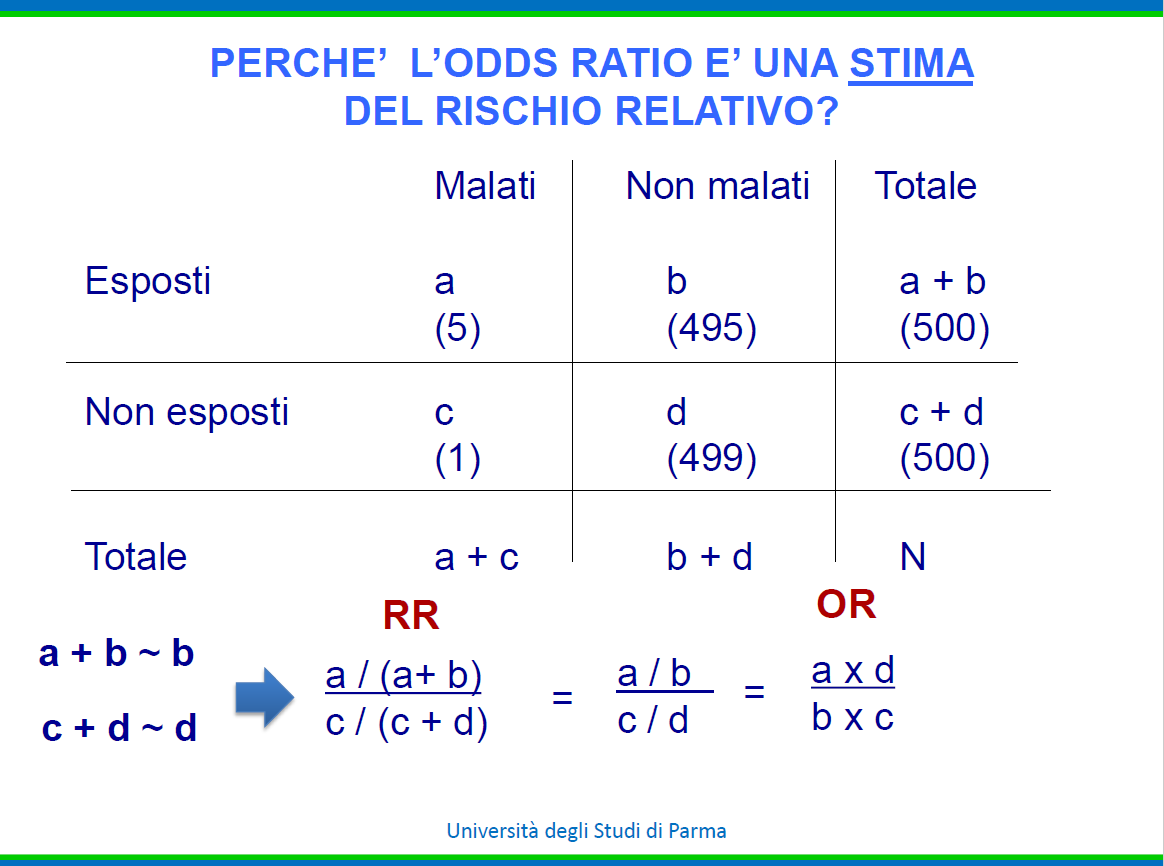
\includegraphics[width=0.8\textwidth]{04/image6.png}
	\end{figure}

L'odds ratio = odds di esposizione nei casi / odds di esposizione nei
controlli

casi: malati esposti/malati non esposti a/c

controlli: controlli esposti/controlli non esposti b/d

quindi odds ratio=a:c / b:d a x d / b x c

\emph{L'odds ratio è una stima del rischio relativo.}

Come si dimostra matematicamente?

Rischio relativo (RR) = a : (a + b) / c : (c + d)

Quindi l'odds ratio è tanto più uguale a RR quanto più (a + b) ha valore
numerico uguale a (b) e allo stesso modo (c + d) è uguale a (d), ovvero
quando i valori (a) e (c) sono bassi in questo modo il risultato sarà
numericamente vicino a quello dell'odds ratio. (vedi figura, uguaglianza
in basso)

Quindi l'odds ratio è tanto più una stima precisa del rischio relativo
quanto più si tratta di una malattia \emph{rara.}

La misura più affidabile è sempre il rischio relativo, ma se non è
disponibile uno studio a coorte, ma solo uno caso-controllo, in cui si
hanno solo il numero degli esposti e dei non esposti in malati e non
malati, allora si calcola l'odds ratio. È tanto più simile al rischio
relativo quanto più la malattia è poco frequente.

Es. primo studio su associazione tra numero di sigarette al giorno e
prevalenza cancro polmone, che era stato fatto proprio su medici.

\begin{figure}[!ht]
\centering
	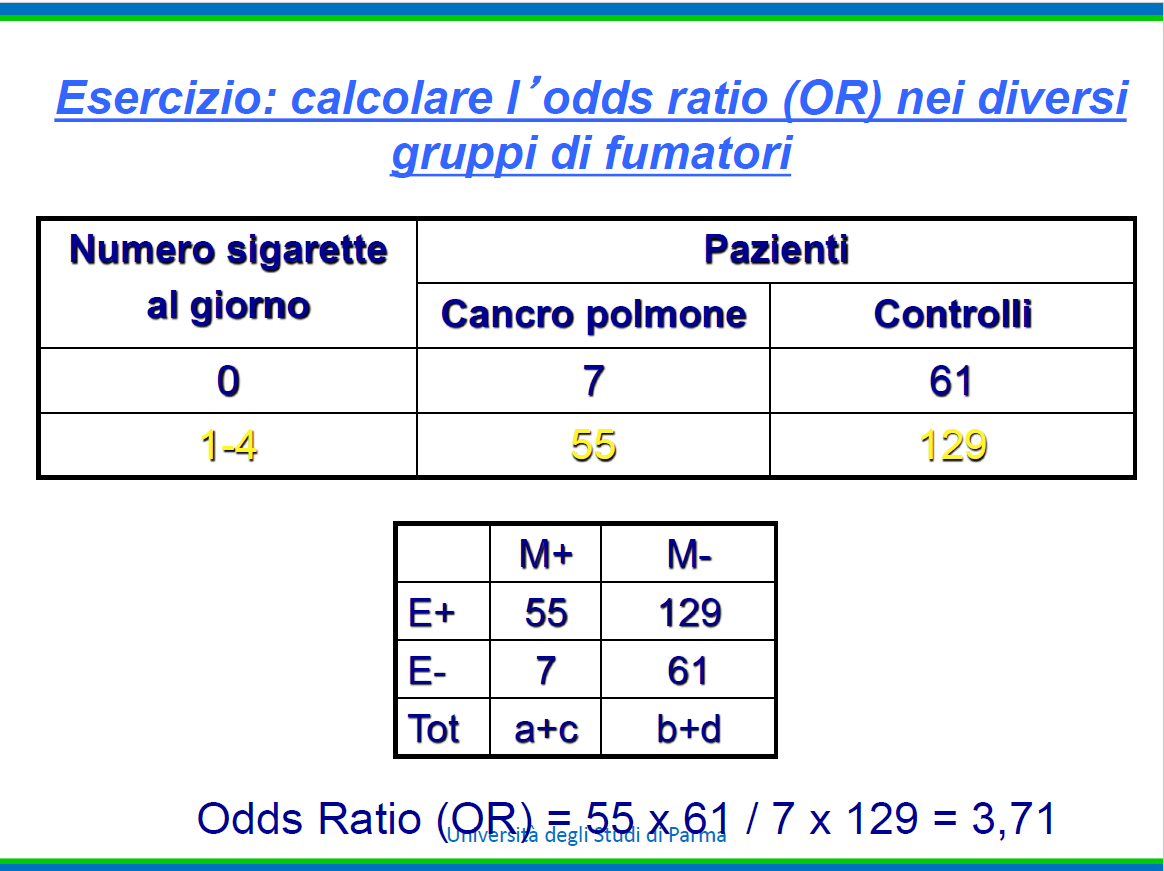
\includegraphics[width=0.8\textwidth]{04/image7.png}
	\end{figure}

Non esposti numero sigarette al giorno= 0; individui con cancro polmone=
7; controlli(sani)= 61

Esposti numero sigarette al giorno= 0-4; individui con cancro polmone=
55; controlli= 129

Quindi 55x61 / 7x129 = 3,71 l'odds ratio di tumore negli esposti è quasi
4 volte maggiore dell'odds di tumore al polmone nei non esposti.

Aumentando esposizione (numero sigarette), aumenta odds ratio patologia:
c'è un effetto dose-risposta.

\subparagraph{Studi Sperimentali}


Negli studi sperimentali si introduce l'esposizione. I più tipici sono i
trials clinici, che valutano l'efficacia di una terapia. Possono essere
trials clinici individuali o anche di comunità.

La maggior parte delle evidenze scientifiche derivano da trials clinici.

\subparagraph{Randomized controller trials }


Si introduce artificialmente un fattore di esposizione, che non è per
forza un fattore di rischio, può anche essere protettivo (ad esempio un
farmaco), in uno solo di due gruppi.

Es. Voglio studiare efficacia di un farmaco oncologico.

Si prende un gruppo di pz oncologici e li si divide in due gruppi: uno a
cui si somministra il trattamento che si vuole studiare e l'altro a cui
non viene somministrato niente oppure viene dato il placebo o un'altra
terapia. Questi gruppi vengono seguiti nel tempo, per un periodo più o
meno lungo di follow up e si valutano i risultati.

Concetto di \textbf{randomizzazione}: l'assegnazione dei pz ai due
gruppi deve essere random, cioè assolutamente casuale, perché i due
gruppi devono essere il più possibile uguali e comparabili e che l'unica
differenza sia nel trattamento, mentre siano uguali per tutte le altre
caratteristiche di età, sesso, comorbidità, ecc... al fine che la
comparazione sia il più possibile oggettiva. Ci sono tecniche di
randomizzazione. Questo limita il più possibile la disomogeneità.

Se questi due gruppi non fossero simili per gravità di patologia, il
rischio sarebbe di avere una sottostima dell'efficacia del trattamento
ad esempio perché si somministra la terapia a pz più gravi.

Caratteristiche:

\begin{itemize}
\item
  sono fatti in condizioni sperimentali
\item
  basso rischio bias e confondimento: sono gli studi ideali, sono quelli
  che più si avvicinano alla verità assoluta, perché lo sperimentatore
  ha la possibilità di introdurre in maniera artificiale l'intervento da
  andare a testare. Sono all'apice della piramide delle evidenze.
\item
  molto complessi
\item
  molto costosi
\item
  aspetti etici: non sempre si può somministrare un trattamento proprio
  per questioni etiche.
\end{itemize}

Gli studi sperimentali sono quelli di approvazione dei farmaci (fase
1,2,3...)

\paragraph{Risultati dei disegni di studio }


I risultati dei disegni di studio vengono \emph{sintetizzati} e
\emph{disseminati} attraverso la letteratura scientifica (i papers) e
costituiscono le \textbf{evidenze scientifiche} sulle quali si basa la
medicina moderna.

Le evidenze scientifiche a cosa servono?

\begin{enumerate}
\def\labelenumi{\arabic{enumi}.}
\item
  a guidare le decisioni cliniche
\item
  ad informare le politiche sanitarie
\end{enumerate}

queste due sono le principali utilità.

\begin{enumerate}
\def\labelenumi{\arabic{enumi}.}
\item
  ad identificare aree dove ulteriori ricerche sono necessarie e quindi
  quesiti di ricerca rilevanti
\item
  ad identificare priorità di ricerca, tematiche, che è prioritario che
  la ricerca approcci
\item
  a sostenere e supportare gli obiettivi di nuovi progetti di ricerca
\item
  interpretare i risultati di un progetto di ricerca
\end{enumerate}

La letteratura scientifica si divide:

\begin{itemize}
\item
  \textbf{primaria}: utilizza dati originali (i disegni di studio)
\item
  \textbf{secondaria}: sintetizza in maniera qualitativa e/o
  quantitativa la letteratura primaria, le evidenze scientifiche
  (metanalisi e revisioni sistematiche).
\item
  \textbf{terziaria}: strumenti per orientare la pratica clinica e le
  politiche sanitarie (utilizzando la letteratura primaria e
  secondaria): linee guida, HTA
\end{itemize}

La letteratura secondaria è fondamentale, perché il numero di evidenze
scientifiche pubblicate su PubMed è enorme e aumenta in maniera
esponenziale.

Le revisioni possono essere narrative e sistematiche. Una
\textbf{revisione narrativa} è un riassunto non sistematico di tutto
quello che viene detto su un argomento; non ha molto valore scientifico
e la sua collocazione sulla piramide delle evidenze non è ai vertici. Le
\textbf{revisioni sistematiche} invece sono ai vertici; sono degli studi
che raccolgono in maniera sistematica e rigorosa tutte le evidenze
disponibili su un determinato argomento.

La \textbf{metanalisi} è l'analisi \emph{quantitativa} di tutte queste
evidenze. La revisione sistematica le raccoglie, la metanalisi le
analizza numericamente. È una tecnica statistica, che mette insieme i
risultati di più studi che hanno approcciato lo stesso argomento.

La revisione sistematica è un tentativo di sintetizzare i risultati di
due o più pubblicazioni su una determinata problematica sanitaria. Viene
realizzata attraverso un approccio scientifico rigoroso ed è un vero e
proprio progetto di ricerca.

Una revisione sistematica può o meno includere una metanalisi. Una
metanalisi è un'analisi statistica dei risultati di studi indipendenti,
che ha generalmente come obiettivo quello di produrre una singola stima
numerica (ad esempio una singola stima di rischio relativo) dell'effetto
di un trattamento, di un intervento.

Es. di metanalisi: impatto del trattamento sulla mortalità espresso come
odds ratio. I diversi studi hanno trovato odds ratio diversi, la
metanalisi consente di mettere numericamente insieme tutti i valori di
odds ratio, tenendo in considerazione anche le dimensioni dei campioni
dei singoli studi, trovando un risultato di odds ratio che li
sintetizza.

Ci sono dei documenti che dicono esattamente quali sono gli step per
fare una revisione sistematica o una metanalisi.

{[}I passi di una revisione sistematica li guardate da soli o saranno
affrontati nella prossima lezione{]}

\begin{figure}[!ht]
\centering
	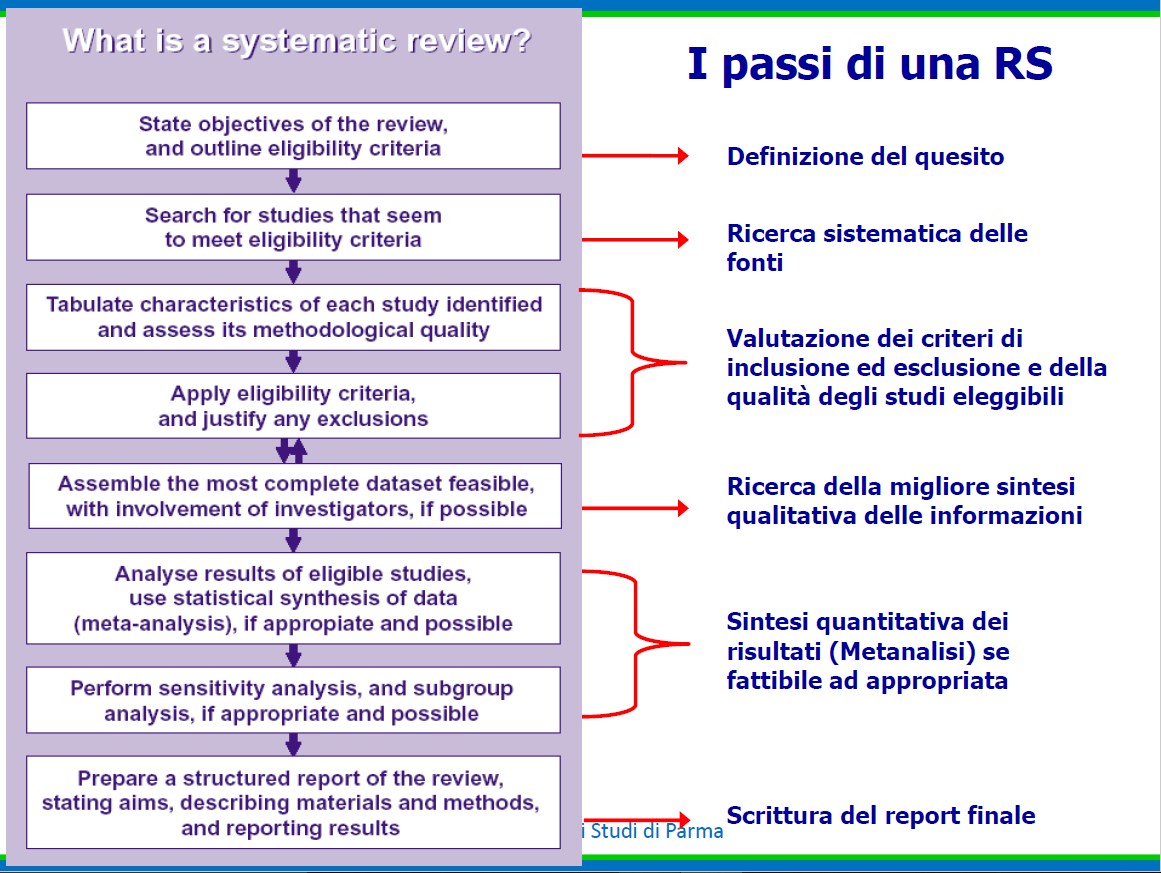
\includegraphics[width=0.8\textwidth]{04/image8.png}
	\end{figure}


{[}Nelle tesi di laurea una revisione sistematica è considerata una
ricerca sperimentale e una metanalisi si può fare anche senza dati, dato
che spesso non sono disponibili, ma se avete un buon quesito di ricerca
potete fare una metanalisi ed è considerata uno studio sperimentale.{]}


\section{Raccomandazioni o Linee Guida}

La funzione della ricerca scientifica e in particolare della ricerca epidemiologica è il beneficio del paziente e il beneficio della comunità (sanità pubblica).

Sono già state trattate a lezione la ricerca scientifica, i disegni di studio, la letteratura primaria e secondaria, le revisione sistematica e metanalisi.

Manca il concetto delle \textbf{\emph{RACCOMANDAZIONI}}.

I ricercatori fanno ricerca, pubblicano il risultato di tali ricerche nelle revisioni sistematiche e tutto questo serve per sviluppare delle \emph{RACCOMANDAZIONI O LINEE GUIDA}. Le linee guida o protocolli vengono stilate da panels di esperti che si basano sulle \textbf{evidenze} della letteratura.

\begin{figure}[!ht]
\centering
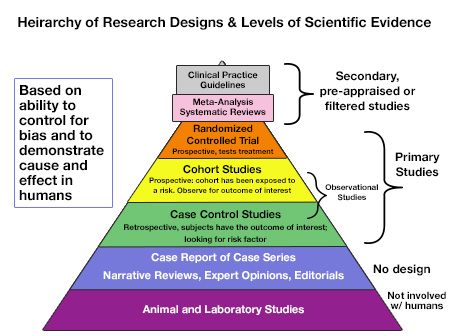
\includegraphics[width=0.7\textwidth]{05/image1.png}
\end{figure}

La \textbf{\emph{piramide delle evidenze}} mostra i vari metodi di studio e di indagine e li va a suddividere a seconda della loro importanza. All'apice della piramide abbiamo le linee guida sulla clinical practice, poi metanalisi e revisioni sistematiche, studi clinici randomizzati e così via.

L'OMS si occupa di stilare le linee guida (che valgono a livello nazionale) attinenti ai vari argomenti clinici e verranno poi implementate a livello degli stati membri.

Arrivare ad una linea guida è un processo molto lungo e che richiede l'azione di più esperti.

\subsection{Medicina basata sulle Evidenze}

La MEDICINA BASATA SULLE EVIDENZE è l'integrazione della migliore ricerca scientifica, con l'aggiunta dell'esperienza clinica del medico e i valori del paziente. (Sackett)

\begin{figure}[!ht]
\centering
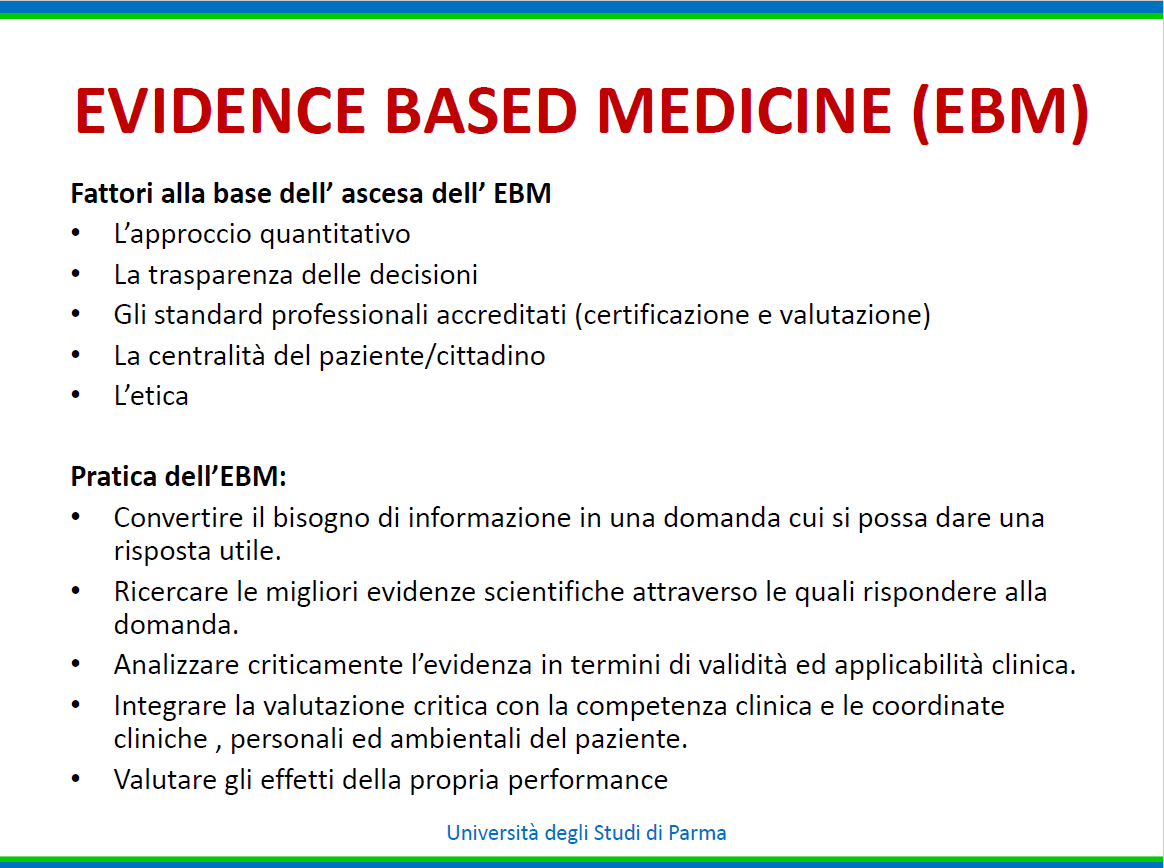
\includegraphics[width=0.7\textwidth]{05/image2.png}
\end{figure}

Tenendo in considerazione ciò che ha detto Sackett, quindi, l'EMB è il risultato di una triangolazione tra:

\begin{itemize}
\item
  applicazione delle evidenze delle ricerche scientifiche
\item
  esperienza clinica da parte del medico
\item
  bisogni clinici e sociali dei pazienti
\end{itemize}

La EMB nasce dalla necessità di sostenere le attività cliniche attraverso principi condivisi di interpretazione dei risultati della ricerca clinica. E' l'uso coscienzioso, esplicito e giudizioso della miglior attuale evidenza scientifica, per prendere decisioni, in relazione all'assistenza sanitaria dei pazienti.

La ricerca scientifica serve ad avere una buona clinica. Qualunque branca della medicina agisce grazie alle evidenze che vengono pubblicate sulle ricerche scientifiche.

\begin{figure}[!ht]
\centering
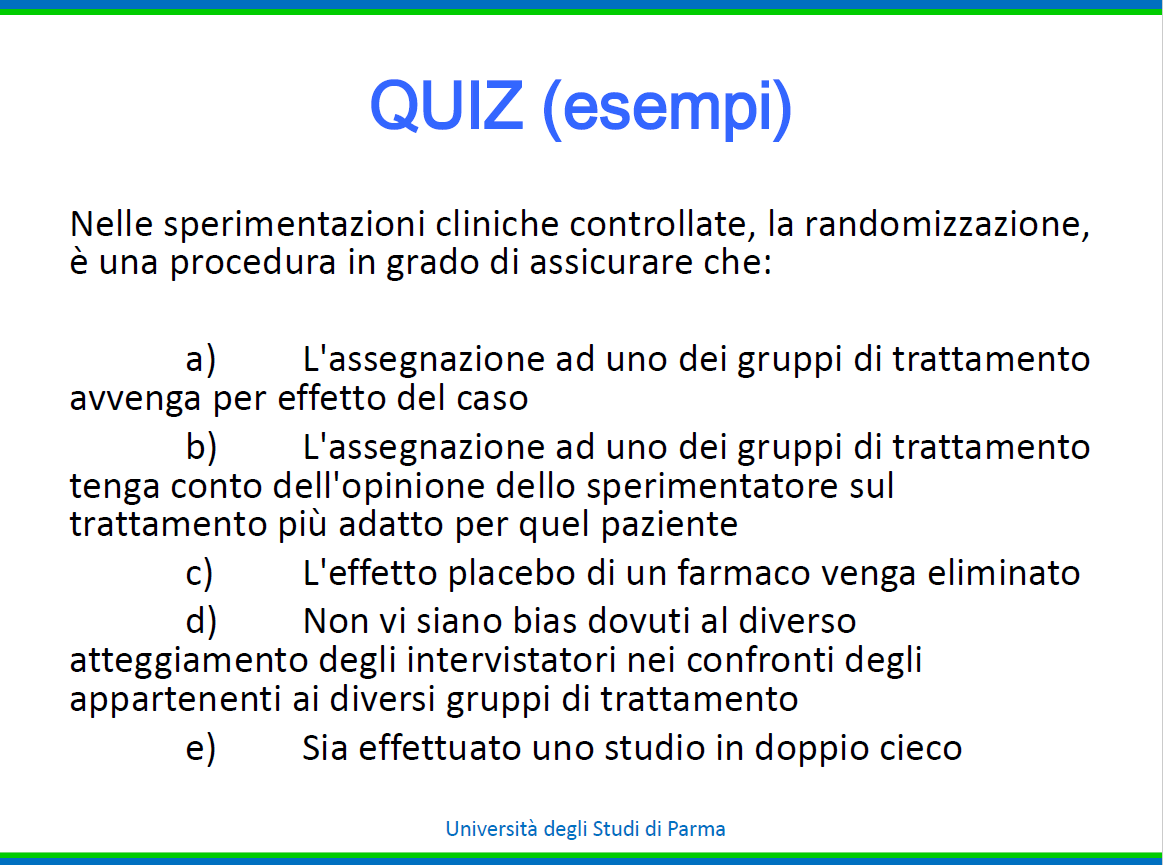
\includegraphics[width=0.7\textwidth]{05/image3.png}
\end{figure}

La risposta corretta è la A.

\begin{figure}[!ht]
\centering
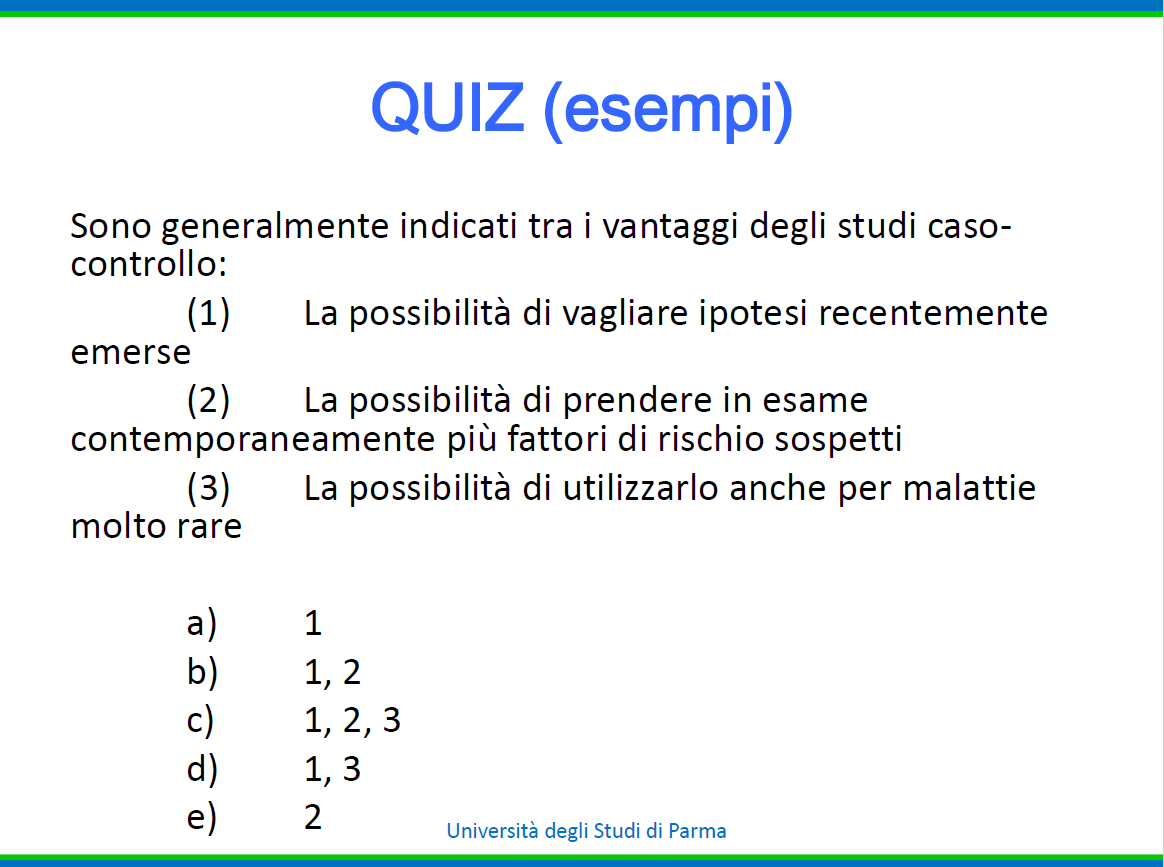
\includegraphics[width=0.7\textwidth]{05/image4.png}
\end{figure}

La risposta corretta è la C.

Lo studio caso-controllo è quello che prende i malati e i non malati e \emph{valuta l'ESPOSIZIONE}. Con questo approccio possiamo \textbf{\emph{indagare più fattori di rischio}} sui malati, mentre \emph{se partiamo dai fattori di rischio} degli esposti e non esposti, sarà \emph{più difficile prendere in considerazione più esposizioni.}

\begin{figure}[!ht]
\centering
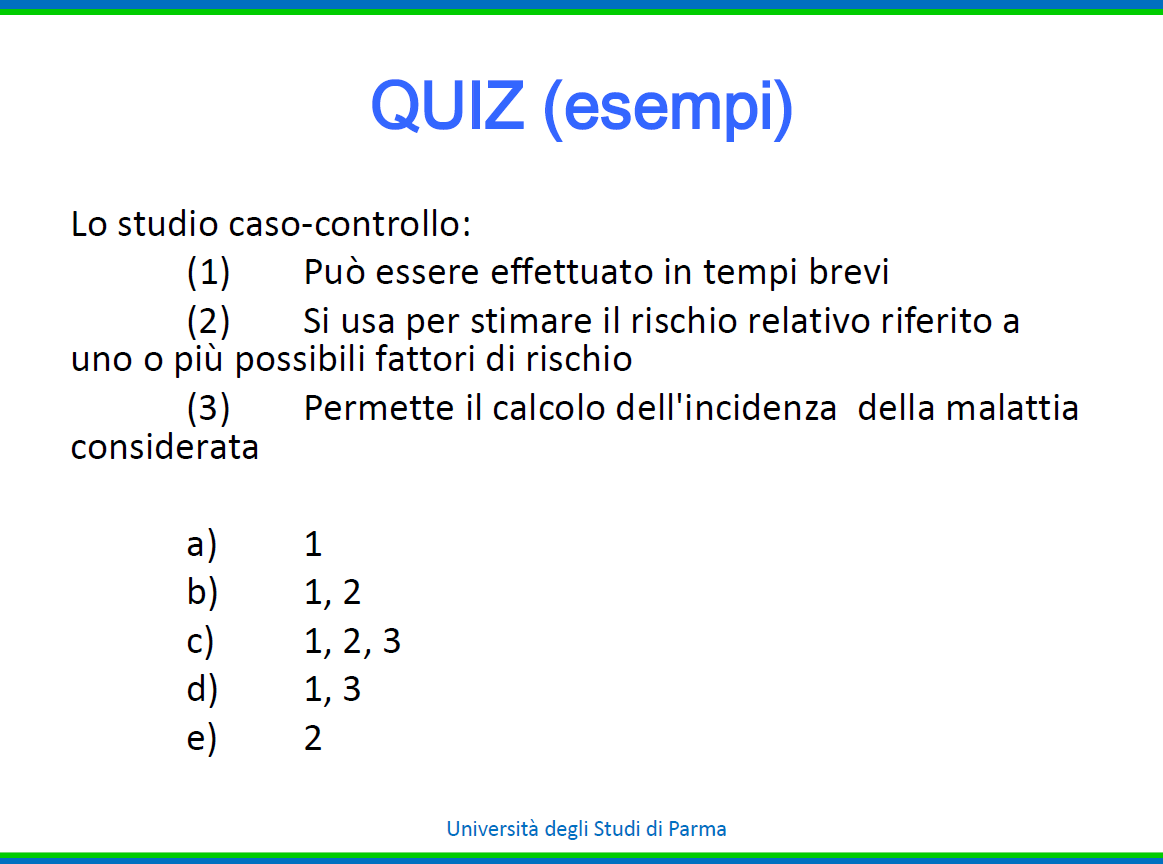
\includegraphics[width=0.7\textwidth]{05/image5.png}
\end{figure}

La risposta corretta è la B.

Lo studio caso-controllo \textbf{\emph{non permette assolutamente il calcolo dell'incidenza della malattia}} considerata. Si calcola in tempi brevi, diversamente da quello che succede con gli studi prospettici.

Non si calcola il rischio relativo degli studi caso-controllo, bensì l'\textbf{\emph{ODDS RATIO}} (che è una stima del rischio relativo, che si avvicina al rischio relativo tanto più la patologia è rara).

\section{Errori in epidemiologia: BIAS e CONFONDIMENTO}

L'obiettivo degli studi epidemiologici di tipo analitico è quello di \textbf{\emph{stimare l'associazione tra un'esposizione e un outcome}}, cioè \textbf{\emph{determinare l'associazione di un fattore di rischio,}} determinante una causa e una patologia di interesse. Gli studi epidemiologici però possono avere degli errori, che possono far si che la stima che si va a calcolare sia errata. Quando si può instaurare l'errore? Può instaurarsi in ciascuno dei passaggi attinenti agli studi epidemiologici, ossia: disegno di studio, raccolta dei dati, analisi e interpretazione dei dati.

\begin{figure}[!ht]
\centering
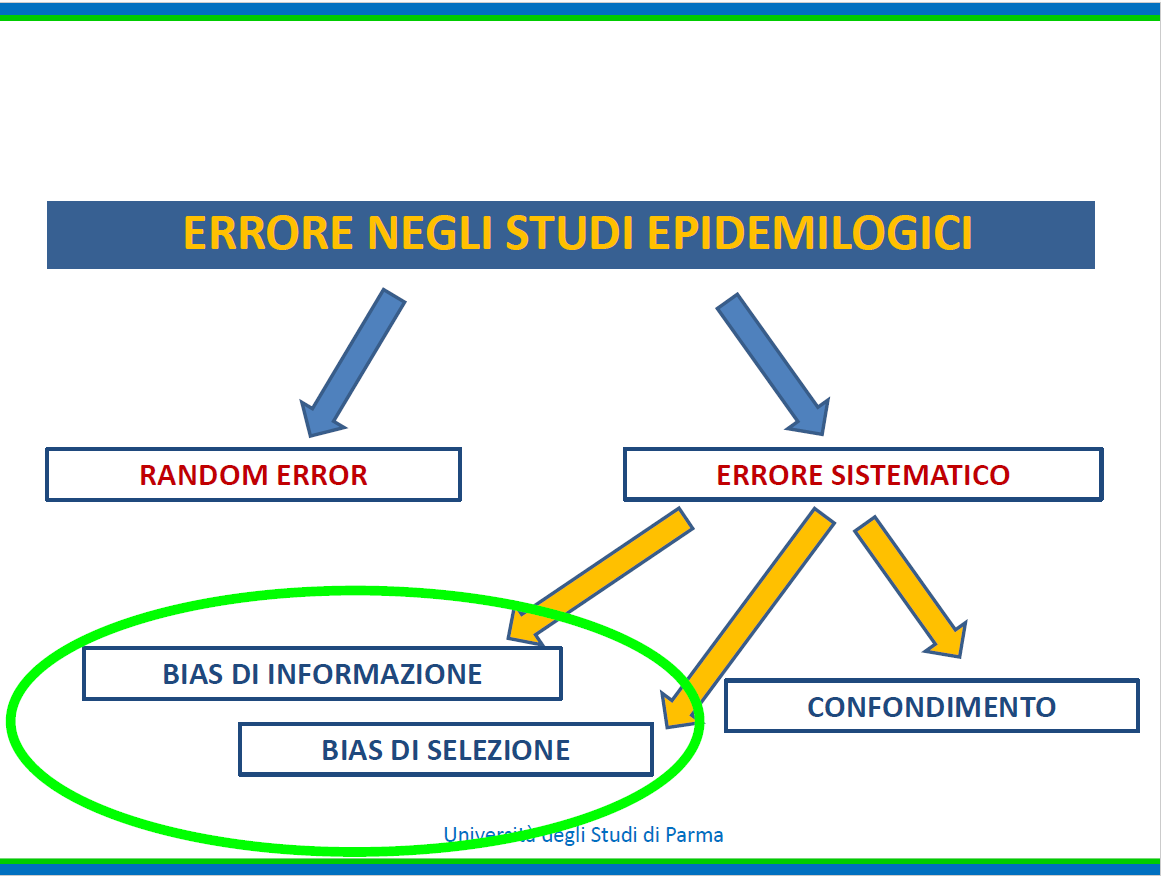
\includegraphics[width=0.7\textwidth]{05/image6.png}
\end{figure}

Tutti gli studi epidemiologici sono potenzialmente a rischio di errore.

Che tipi di errori ci sono? \textbf{\emph{ERRORE RANDOM e ERRORE SISTEMATICO}}

\subsection{Errore Sistematico}

Esso è costituito da due diverse categorie: \textbf{\emph{BIAS e CONFONDIMENTO. }}

Il BIAS è una deviazione dei risultati dal vero; è qualsiasi trend nella raccolta, interpretazione, analisi e review dei dati, che può portare a conclusioni sistematicamente differenti dalla realtà.

Quindi:

\begin{itemize}
\item
  il bias è una forma di distorsione introdotta nei risultati
\item
  i bias possono essere prevenuti attraverso un adeguato disegno sperimentale e una corretta esecuzione dello studio
\item
  i bias non si possono evitare attraverso l'ampliamento della casistica (non dipendono dal numero del campione).
\end{itemize}

I bias sono errori che si instaurano nelle fasi di disegno di studio e nella raccolta dei dati.

Non si può fare molto per minimizzare i bias a livello di analisi dei dati (una volta che i dati sono stati raccolti). Questo è il motivo per cui è necessario spendere adeguate risorse per evitare i bias durante la fase di pianificazione dello studio. I BIAS si suddividono a loro volta in varie categorie:

\paragraph{Bias di Selezione}

Fa riferimento a come gli individui vengono selezionati per prendere parte ad uno studio:

Gli individui selezionati sono rappresentativi della popolazione che si vuole studiare?

\begin{itemize}
\item
  \textbf{\emph{negli studi CASO-CONTROLLO:}} il problema più importante è la selezione dei controlli. Esempi? L'esposizione che si vuole studiare è associata alla probabilità di essere selezionata come controllo. In questo caso i controlli NON sono rappresentativi della popolazione che si vuole studiare.
\end{itemize}

Il bias di selezione fa riferimento ad un \emph{errore} non nella selezione dei casi che vengono selezionati in base all'outcome, bensì \emph{nella selezione dei controlli}.

La selezione dei controlli è in qualche modo associata all'esposizione che si vuole studiare. Ad esempio, vogliamo studiare l'associazione tra fumatori e malati di tumore al polmone. La ricerca dei casi non è difficile: basta prendere i malati di tumore al polmone, dopodichè bisogna valutare una popolazione di controllo sulla quale andare a valutare l'esposizione al fumo per calcolare l'odds ratio quale stima del rischio relativo (odds ratio: valutazione dell'esposizione nei casi e valutazione di esposizione nei controlli, poi si fa il rapporto e tale rapporto rappresenta l'odds ratio, che è uguale, a livello interpretativo, al rischio relativo. Se il risultato è > 1 diciamo che l'esposizione di interesse è un fattore di rischio, se invece il rischio relativo risulta < di 1, l'esposizione di
interesse sarà un fattore protettivo).

Possiamo prendere 100 controlli in via Farini, ad esempio, o 100 controlli in un reparto di ospedale (non in un reparto di oncologia, bensì in un qualsiasi altro reparto). Con questi due tipi di controlli si va a calcolare il rischio relativo. Il calcolo dell'odds ratio come sarà? Si avrà un rischio di neoplasia maggiore nei controlli ospedalieri: è possibile infatti, che i controlli selezionati in ospedale siano più malati rispetto a quelli di via Farini. Il modo in
cui noi andiamo a selezionare i controlli influisce sull'odds ratio!

Ripetendo: non abbiamo nessun problema a selezionare i casi, in questo caso (malati di tumore oppure non malati). La selezione dei controlli (persone sane) è invece difficoltosa! Dobbiamo \textbf{\emph{prendere la popolazione più generale possibile}}, che sia cioè \textbf{\emph{il più
lontano possibile dall'essere un caso}}.

Di solito negli studi caso-controllo, i controlli vengono scelti in ambito ospedaliero, perchè è più semplice, rapido e meno dispendioso in termini economici, ma questo introduce un BIAS DI SELEZIONE. Se invece i
controlli venissero selezionati in modo random nella popolazione
generale, questo si avvicinerebbe di più ad uno studio di tipo
sperimentale. I controlli presi in ambito ospedaliero, infatti,
inficiano la stima relativa dell'odds ratio, perchè sono persone
caratteristicamente diverse dalla popolazione generale, solitamente con
più patologie e morbilità associate. Il fatto di essere in ospedale può
anche condizionare determinate caratteristiche dei pazienti.

\begin{itemize}
\item
  \textbf{\emph{negli studi A COORTE:}} è minore in quanto l'inclusione
  di esposti e non esposti precede l'insorgenza nell'outcome. \emph{Si
  selezionano i pazienti in base all'esposizione (esposti e non esposti)
  e si studia l'insorgenza dell'outcome. }
\end{itemize}

Nel trials, che è la situazione sperimentale per eccellenza, il rischio
di bias è minimo, tranne nei casi in cui ci sia una perdita di follow up
maggiore tra le persone sottoposte all'intervento e le persone presenti
nel gruppo di controllo.

\paragraph{Bias di Informazione}

Fa riferimento alla \textbf{\emph{MISCLASSIFICAZIONE tra esposizione/non
esposizione e/o outcome/non outcome.}} Si deve considerare il fatto che,
in questo tipo di studi, i soggetti malati hanno la tendenza a ricordare
l'esposizione maggiore rispetto ai non malati. Quindi risulta una non
veritiera maggiore esposizione che porta ad una \textbf{\emph{sovrastima
del rischio relativo}}.

\begin{figure}[!ht]
\centering
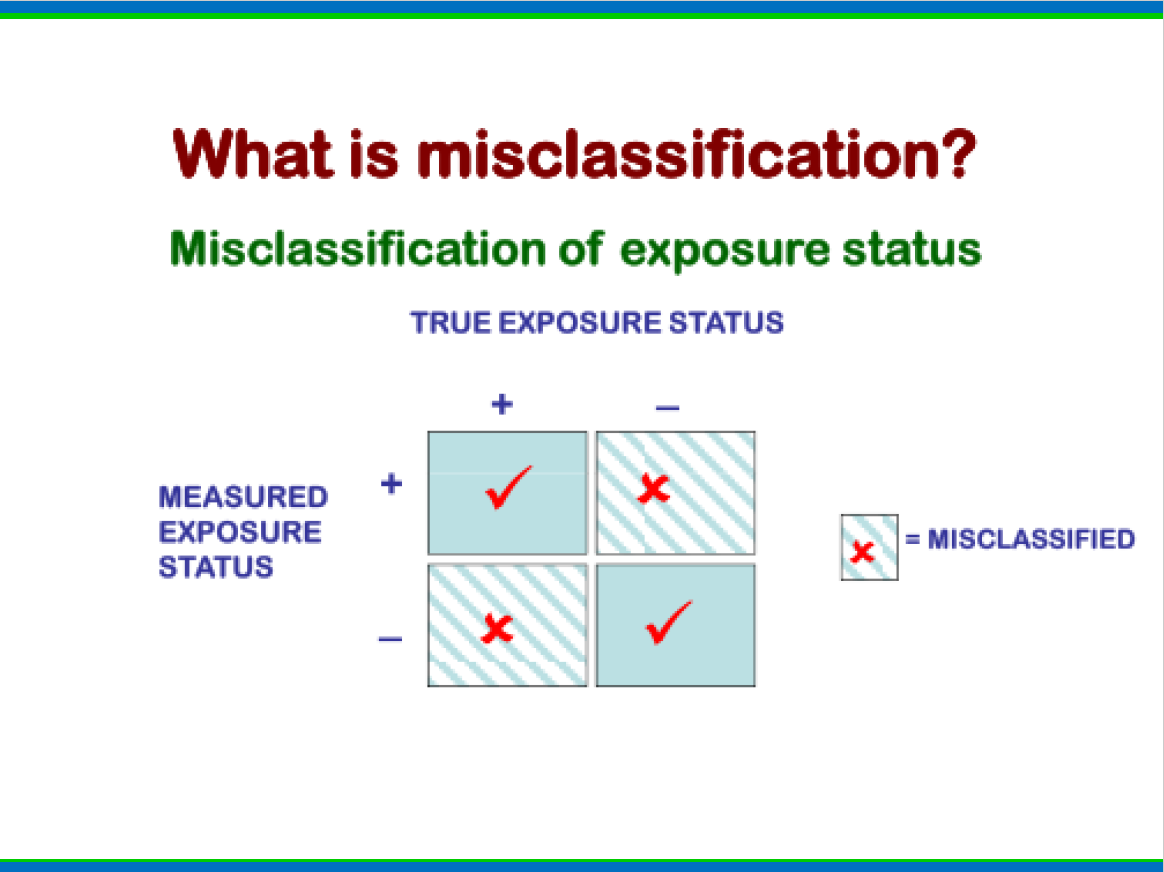
\includegraphics[width=0.7\textwidth]{05/image7.png}
\end{figure}

Guardando l'immagine, lungo la colonna si vede la \emph{vera
esposizione}. Ad esempio: fumatori sì, fumatori no.

Lungo le righe: \emph{esposizione riportata}. Esempio: dicono di essere
fumatori, non dicono di essere fumatori (è difficile non ricordarsi se
si è fumatori oppure no, ma questo è solo un esempio per far capire).

Se l'incrocio tra righe e colonne porta ad un risultato diverso, si
tratta di MISCLASSIFICAZIONE.

Vera esposizione, riportare l'esposizione in maniera corretta; vera non
esposizione, riportare la non esposizione in maniera corretta: queste
sono delle classificazioni corrette. Non lo sono se ad esempio
l'esposizione non c'è ma viene erroneamente riportata.

Questo non si fa per gli studi a coorte perchè, in quel caso, al tempo
0, non c'è nessun malato (persone tutte sane che vanno divise per
diversa esposizione).

Il bias di informazione è perciò un erroneo riportare l'esposizione.
Esso può essere:

\begin{itemize}
\item
  \textbf{\emph{CASUALE}}
\item
  \textbf{\emph{NON CASUALE}}
\end{itemize}

Se è casuale (indipendente dall'outcome o indipendente
dall'esposizione), è semplicemente un errore di misurazione.

Se invece l'errore non è random e se è influenzato dall'outcome e
dall'esposizione, si dice \textbf{\emph{DIFFERENZIALE.}}

Es: stiamo studiando un farmaco che si pensa riesca a curare macchie
cutanee. Vengono presi due gruppi per lo studio: gruppo di malati (con
le macchie cutanee) a cui diamo il farmaco e gruppo di malati a cui non
lo diamo. Dopo un po' di giorni andiamo a vedere l'outcome. Si vede che
le macchie sono diminuite nei pazienti che hanno preso il farmaco. Si
valuta il rapporto della diminuzione delle macchie nei pazienti che
hanno preso il farmaco e il rapporto della diminuzione nei pazienti che
non hanno preso il farmaco. In questo modo si vede l'efficacia del
farmaco.

A volte però l'outcome di interesse non è così oggettivabile: ad esempio
nel caso dei trattamenti con farmaci antidepressivi. Ad un gruppo di
depressi si somministra il farmaco, all'altro gruppo si somministra il
placebo. In questo caso, se io so quale sia il gruppo a cui è stato
somministrato il placebo e quale a cui sia stato somministrato il
farmaco, in una situazione non oggettivabile come questa (lo stato
d'animo dei pazienti), ne potrei essere influenzato e potrei alterare lo
studio.

\emph{\textbf{Bias di informazione di tipo differenziale}: tendo a
considerare come più guarito il paziente che è stato sottoposto al
trattameno. Questo porta ad una sovrastima dell'effetto del farmaco}.

Se invece fossi ignaro riguardo alla suddivisione dei due gruppi, questo
non andrebbe a inficiare sulla valutazione.

Gli effetti della misclassificazione possono quindi essere differenziali
o non differenziali. Se \textbf{\emph{non differenziali, cioè random}},
la stima dell'associazione tra esposizione e outcome è ``biased towards
unity'': \textbf{\emph{l'effetto dell'esposizione è cioè sottostimato.}}

Se invece l'effetto della misclassificazione è
\textbf{\emph{differenziale}}, la stima di associazione tra esposizione
e outcome può essere \textbf{\emph{sia sovra che sottostimato}}, in base
alle circostanze.

\begin{figure}[!ht]
\centering
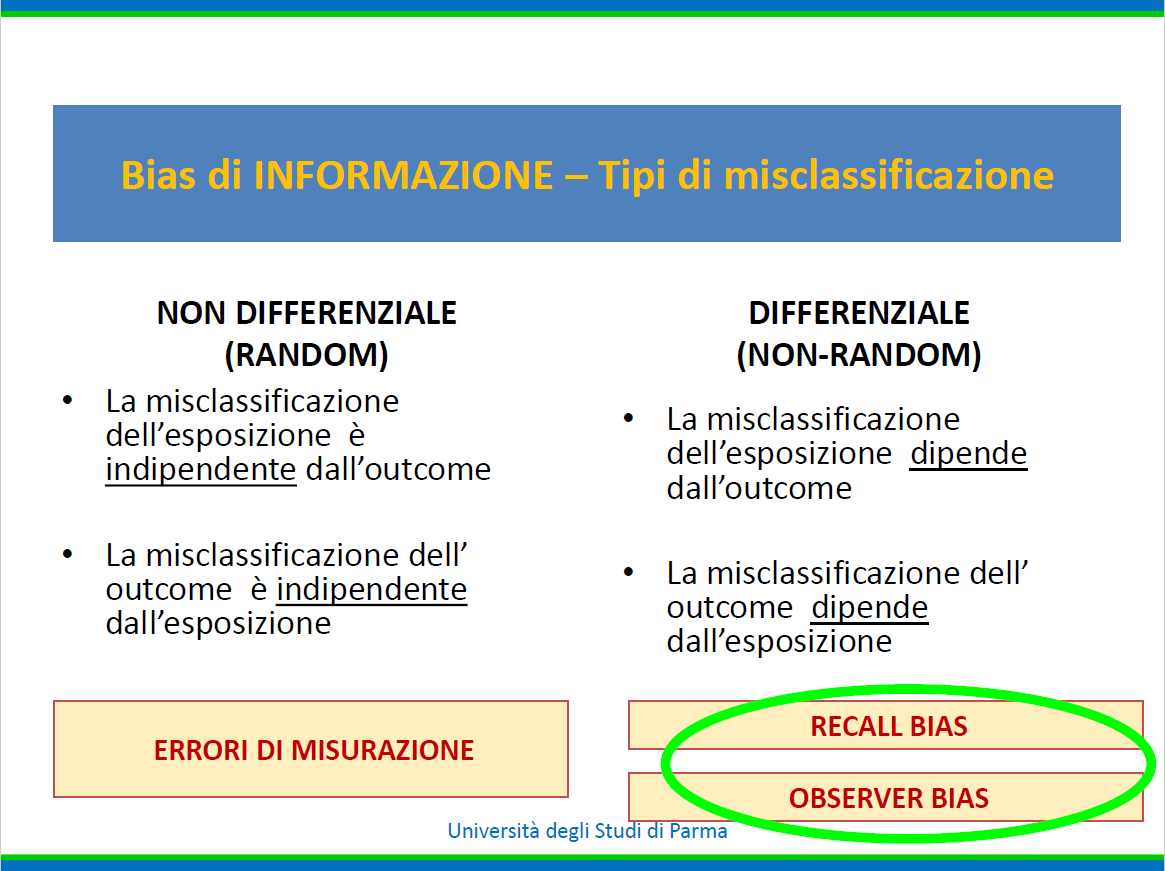
\includegraphics[width=0.7\textwidth]{05/image8.png}
\end{figure}

Il \textbf{RECALL BIAS} è quello del ricordo dell'esposizione; è un
sottotipo di bias di informazione.

E' tipico degli studi caso-controllo; l'accuratezza e l'attendibilità
dell'informazione riportata (e ricordata) dai CASI è superiore a quella
dei CONTROLLI.

COME SI PUO' MINIMIZZARE questo bias?

\begin{itemize}
\item
  facendo interviste standard ai casi ed ai controlli
\item
  usando fonti di dati ogettivi (cartelle cliniche)
\item
  validando il campione delle risposte
\end{itemize}

Ricapitolando: il bias differenziale è in base all'outcome e
all'esposizione. E' un bias che non dipende da errori di misurazione
random, ma è associato al fatto di essere un caso o un controllo: la
misclasificazione è legata allo status di caso, al fatto di essere un
caso o un controllo.

Errore DIFFERENZIALE : la selezione o l'info è sbagliata in maniera
direttamente legata al fatto di essere un caso, un controllo; un
esposto-non esposto.

Errore NON DIFFERENZIALE: l'errore è indifferentemente, in maniera
random, distribuito tra le categorie studiate.

Un esempio classico di information bias, che misclassifica l'esposizione
in base al fatto di essere casi o controlli, è proprio un caso di errore
differenziale, che porta i casi, in maniera differenziale, a
sovrastimare l'esposizione.

Non si tratta di errori di analisi, bensì di errori che avvengono
durante l'attuazione dello studio. L'analisi è un processo in cui non si
verrà più a contatto con i pazienti, ma si studieranno i dati già
ricavati e già opportunatamente trascritti in tabelle excell. Se in fase
di implementazione dello studio sono stati raccolti dei dati sbagliati,
in fase di analisi, ormai, non avrò più la possibilità di minimizzare i
bias.

L' \textbf{OBSERVER BIAS} è un altro tipo di bias d'informazione in cui
l'errore sistematico è dell'osservatore che classifica in base al fatto
che sa a quale gruppi sono stati assegnati i vari soggetti:

\begin{itemize}
\item
  il ricercatore raccoglie dati sull'esposizione in maniera diversa tra
  casi e controlli
\item
  il ricercatore fa diagnosi di outcome in maniera diversa tra
  esposti/non esposti
\end{itemize}

IL RICERCATORE è INFLUENZATO DALL'IPOTESI DI RICERCA.

Come minimizzarlo?

\begin{itemize}
\item
  rendere il ricercatore cieco sullo status di caso/controllo dei
  soggetti (difficile nel caso visto prima, ad esempio, sulle macchie
  cutanee)
\item
  mascherare nei questionari l'ipotesi di ricerca
\item
  utilizzo di misure oggettive e protocolli standard
\item
  training degli operatori
\end{itemize}

\begin{figure}[!ht]
\centering
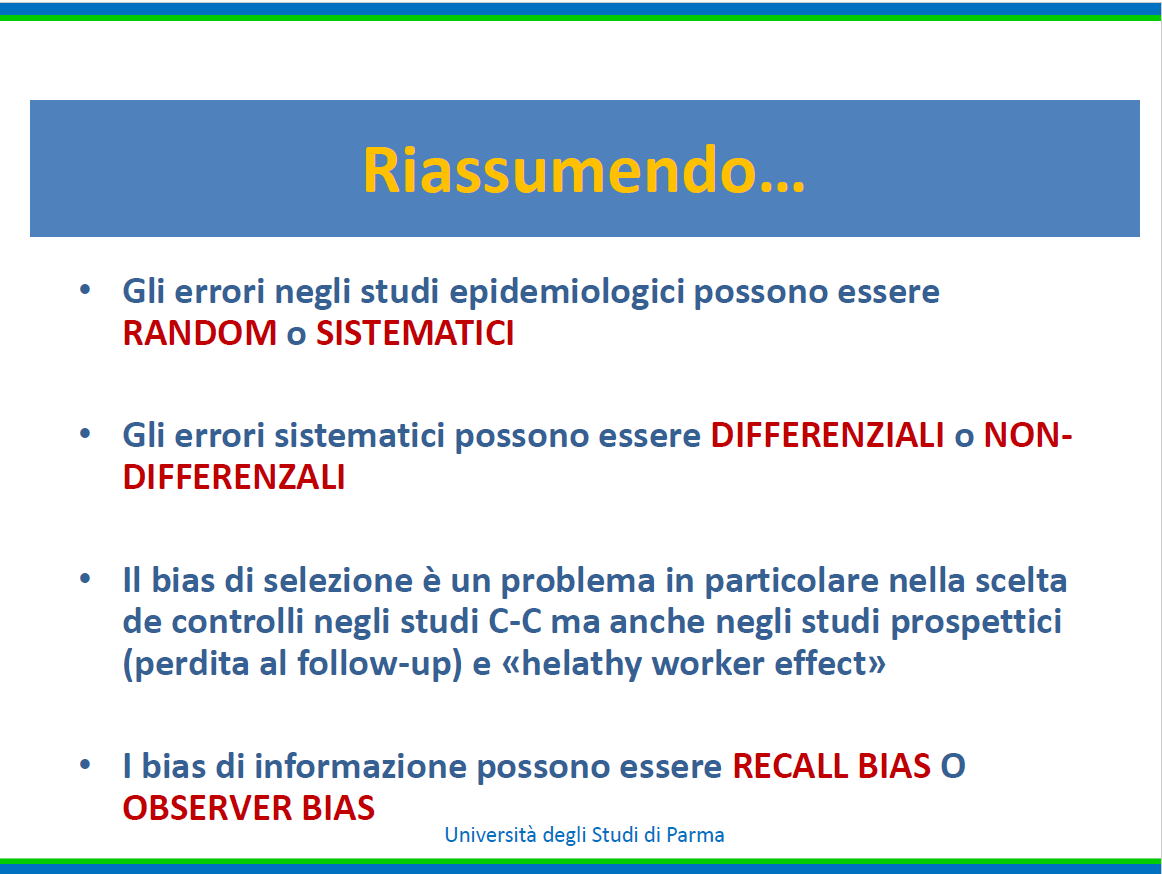
\includegraphics[width=0.7\textwidth]{05/image9.png}
\end{figure}

BIAS DI SELEZIONE, BIAS DI INFORMAZIONE (RECALL BIAS E OBSERVER BIAS,
errore sistematico dell'osservatore che classifica in base al fatto che
sa l'appartenenza dei soggetti ai vari gruppi).

\subsection{Confondimento}

E' un fattore associato sia all'esposizione sia all'outcome.

Se è presente un fattore associato sia all'esposizione che all'outcome e
noi non lo prendiamo in considerazione, sbagliamo.

Es. Vogliamo studiare l'associazione tra colore dei capelli grigi e
presenza di patologia cronica degenerativa. Si prende un gruppo di
persone con i capelli grigi e un gruppo di persone con i capelli di
altri colori e si studia l'insorgenza di patologie cronico-degenerative.
Si scopre che l'incidenza di questo tipo di patologie è proprio più alta
in chi ha i capelli grigi. Quindi, l'avere i capelli grigi è un fattore
di rischio? Assolutamente no! C'è un confondimento, sia legato
all'esposizione, sia all'outcome. Tale confondimento potrebbe essere
l'età. Se tenessi conto dell'età, troverei un rischio relativo attorno
all'uno e che quindi mi indicherebbe che il fatto di avere i capelli
grigi di per sè, non è un fattore di rischio.

Il confondimento può essere eliminato in fase di analisi. Si può
eliminare con delle tecniche statistiche multivariabili che riescono a
valutare il rischio relativo tra capelli grigi e patologia tenendo conto
dell'età, oppure stratificando in vari gruppi di età diverse. Facendo
ciò si va a minimizzare il confondimento.

Non sempre è così facile andare a valutare quale sia il fattore di
confondimento. Ci possono essere molteplici fattori che influenzano i
miei dati, oltre all'età: ad esempio: lo stato socio-economico,
l'istruzione, il peso, varie comorbidità. In fase di analisi, gli studi
migliori sono quelli che tengono in considerazione questi vari possibili
fattori di confondimento e che riescono a denaturare l'analisi,
minimizzandola all'effetto dell'esposizione di interesse e all'outcome.

L'epidemiologia cerca di stimare i determinanti, le varie cause, tenendo
sempre in considerazione tutti i possibili fattori di confondimento.

\subsection{Errore Random}

Noi vogliamo studiare quello che avviene a livello di popolazione, ma
quello che in realtà facciamo è \emph{studiare un piccolo campione di
popolazione} (\textbf{errore campionario}). Per questo motivo, un errore
in questi studi c'è sempre, ed è un errore affidato al caso. In fase di
disegno di studio questo errore non si può eliminare: è INELIMINABILE.
E' stimabile con tecniche statistiche in fase di analisi.

L'errore casuale è tanto più grande quanto più piccolo è il campione.

L'errore sistematico di selezione è un errore che viene fatto in fase di
disegno e conduzione dello studio. Lo si può minimizzare con degli
accorgimenti, in fase di analisi, ma non eliminare del tutto.

\section{Lo sviluppo di un farmaco}

\begin{figure}[!ht]
\centering
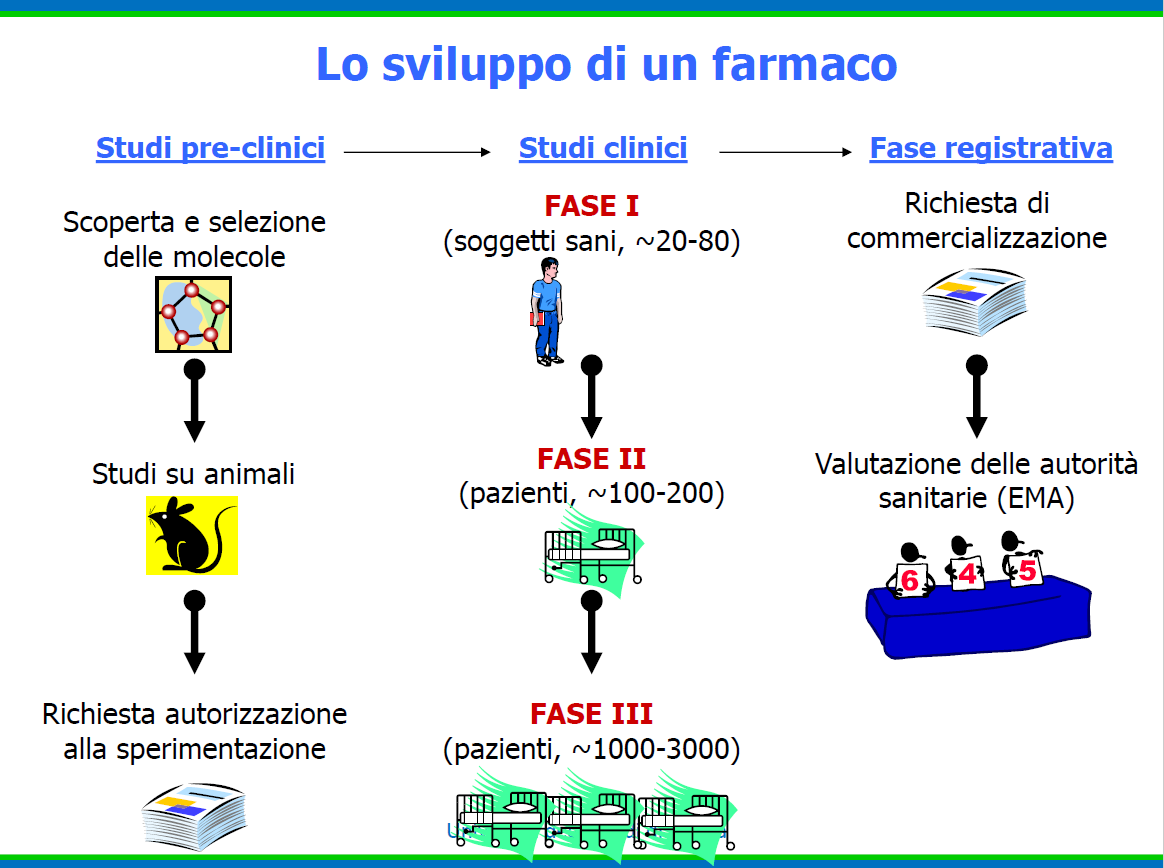
\includegraphics[width=0.7\textwidth]{05/image10.png}
\end{figure}

Le fasi per lo sviluppo di un farmaco sono tre:

\begin{itemize}
\item
  studi clinici
\item
  studi pre-clinici
\item
  fase registrativa
\end{itemize}

Gli studi pre-clinici sono quelli che vengono fatti sugli animali,
terminati i quali sarà possibile richiedere l'autorizzazione per la
sperimentazione, dando così inizio alla fase successiva.

Gli studi clinici si dividono in: fase 1, fase 2, fase 3, tra le quali
varierà il numero di soggetti sottoposti allo studio.

Nella fase di registrazione abbiamo la richiesta di commercializzazione
di un farmaco, che verrà valutata dalle autorità nazionali, tra le
quali, a livello Europeo, abbiamo l'EMA (European Medicine Authority),
mentre in Italia abbiamo l' AIFA (agenzia Italiana del farmaco).

Per alcuni farmaci è richiesta l'autorizzazione a livello Europeo, per
altri, a livello Nazionale.

Gli studi clinici di \textbf{fase 1} hanno una durata di un anno o due,
vengono fatti su soggetti di età compresa tra i 20 e 80 anni, volontari
sani. Vanno a studiare:

\begin{itemize}
\item
  la tollerabilità e sicurezza di un farmaco
\item
  i dati di farmaco-cinetica
\item
  i dosaggi ottimali da impiegare durante la fase 2
\end{itemize}

Anche gli studi di \textbf{fase 2} hanno una durata di 1 o 2 anni.
Vengono svolti su di un numero maggiore di soggetti (centinaia).
Valutano:

\begin{itemize}
\item
  l'efficacia e la tollerabilità del farmaco nei PAZIENTI (cioè in
  soggetti malati)
\item
  l'individuazione del rapporto dose-effetto
\end{itemize}

Gli studi di \textbf{fase 3} sono studi più lunghi (3-4 anni), vengono
fatti su più pazienti (1000-3000), per:

\begin{itemize}
\item
  la valutazione di efficacia e tollerabilità su di un campione AMPIO
\item
  definizione finale tra dose ed effetto
\item
  confronto tra trattamenti diversi
\end{itemize}

Gli studi di \textbf{fase 4} sono quelli di post-marketing e sono i più
lunghi in assoluto: durano per sempre. I soggetti interessati sono tutti
coloro che vengono sottoposti ad un determinato trattamento. Gli
obiettivi sono:

\begin{itemize}
\item
  rilevazione di risposte rare/eventi avversi
\item
  effetto dell'interazione con altri farmaci
\end{itemize}

Quando sono nati i trials clinici? Il primo trial è stato effettuato nel
1948, per il trattamento della tubercolosi, con la STREPTOMICINA. I
soggetti sottoposti allo studio avevano un'età compresa tra i 15 e i 25
anni ed erano randomizzati. Si fece l'analisi dei risultati dopo 6 mesi
di trattamento.

\begin{figure}[!ht]
\centering
\includegraphics[width=0.7\textwidth]{05/image11.png}
\end{figure}

\subsection{Criteri per una corretta sperimentazione clinica sui farmaci}

\begin{figure}[!ht]
\centering
\includegraphics[width=0.7\textwidth]{05/image12.png}
\end{figure}

\textbf{1. Presenza di un gruppo di controllo}

Per gli studi epidemiologici è fondamentale la presenza di un
\textbf{\emph{gruppo di controllo}}. Questi gruppi di controllo possono
essere di tipi diversi:

\textbf{Gruppi paralleli}: gruppo A che fa un trattamento, gruppo B che
assume un altro farmaco o placebo, seguiti nel tempo

\textbf{Disegno cross-over}: ciascun gruppo riceve lo stesso trattamento
in fasi successive del trials. E' questo un disegno di studio più
complicato. I suoi:

\begin{itemize}
\item
  \textbf{vantaggi} sono: minor variabilità, miglior utilizzo del
  campione.
\item
  \textbf{svantaggi}: si può applicare solo in determinati trattamenti
  (soprattutto cronici) e la difficoltà di studio è maggiore rispetto a
  quella dei gruppi paralleli.
\end{itemize}

\begin{figure}[!ht]
\centering
\includegraphics[width=0.7\textwidth]{05/image13.png}
\end{figure}

\textbf{2. BLINDNESS, CECITA'}

Ci può essere a due livelli: a livello del paziente, che non sa a che
gruppo è stato assegnato (\textbf{singolo} \textbf{cieco}) e anche a
livello dello sperimentatore (\textbf{doppio cieco}). Questo impedisce
di essere influenzati dalle aspettative che si hanno da un determinato
trattamento. Altrettanto importante è essere ciechi sulla analisi e
valutazione degli studi.

\textbf{3. RAPPRESENTATIVITA' del campione}

Il campione sul quale noi facciamo ricerca è assimilabile alla
popolazione a cui vogliamo assegnare le conclusioni del nostro studio:

\textbf{3A. CRITERI DI INCLUSIONE ED ESCLUSIONE DEI PAZIENTI}

A partire dalla popolazione generale noi applichiamo dei criteri di
eleggibilità e otteniamo la popolazione oggetto di studio. Reclutiamo
attivamente dei pazienti e abbiamo il campione. Facciamo degli studi sul
campione, ma vogliamo che i risultati dello studio si riferiscano alla
popolazione generale. Questo concetto si definisce
\textbf{\emph{INFERENZA STATISTICA}}. Ossia: \emph{la popolazione è la
collettività di soggetti oggetto di studio. Il campione è invece il
gruppo di soggetti estratti dalla popolazione.}

La casualità del campione permette di utilizzare le procedure
dell'inferenza statistica trasferendo i risultati alla popolazione.

Il problema dei trials è la definizione della popolazione (criteri di
inclusione ed esclusione) e l'estrapolazione dei risultati ad una
popolazione più generale rispetto a quella oggetto di studio.

\textbf{3B. La randomizzazione dei pazienti}

E' una caratteristica fondamentale dei trials clinici. I pazienti,
reclutati sulla base dei criteri di inclusione ed esclusione statistici,
vengono assegnati al gruppo di trattamento o di controllo mediante una
forma più o meno sofisticata di sorteggio o randomizzazione (il pc
genera sequenze numeriche casuali).

La randomizzazione deve rendere imprevedibile a quale trattamento verrà
assegnato il paziente successivo. In questo modo si riescono ad ottenere
dei \emph{gruppi omogenei} tra di loro per tutte le caratteristiche note
ed ignote, \emph{ad esclusione del trattamento}: i due gruppi saranno
omogenei, eccezion fatta per il trattamento testato.

L'omogeneità sarà maggiore in relazione alla numerosità del campione.

Insieme alla randomizzazione viene spesso applicata la
\textbf{\emph{STRATIFICAZIONE DEL CAMPIONE }}

\begin{figure}[!ht]
\centering
\includegraphics[width=0.7\textwidth]{05/image14.png}
\end{figure}

Se ci interessa sapere se i risultati dello studio sono validi in
maniera stratificata, cioè se il trattamento ha lo stesso effetto, ad
esempio, sui maschi e sulle femmine, prima di randomizzare i pazienti li
stratifichiamo per età, per genere, per sesso (in pratica per la
stratificazione che ci interessa valutare).

I risultati di uno studio sono estrapolabili solo ai soggetti con le
stesse caratteristiche dei reclutati. Se facciamo uno studio riferendoci
ad una particolare etnia, lo studio può essere estrapolabile anche ad
una etnia diversa da quella studiata? No!

E' quindi opportuno scegliere criteri di inclusione non troppo rigidi,
perchè altrimenti non si avrebbe la certezza che i dati ottenuti
potrebbero andare bene anche su altre popolazioni.

Molto spesso vengono esclusi dalla ricerca donne in gravidanza, anziani,
bambini.... che sono comunque pazienti che spesso usano proprio quei
farmaci in corso di studio!

\textbf{4. DIMENSIONE DEL CAMPIONE}

La numerosità del campione deve essere tale da rispondere
all'obiettività dello studio. Non dovrebbero mai essere arruolate più
persone di quelle necessarie. Ci sono degli studi statistici che mi
permettono di calcolare quanto grande dovrebbe essere il mio campione:
\textbf{\emph{CALCOLI SUL POTERE STATISTICO DELLO STUDIO.}}

\subsection{Outcome o End Points}

Ci sono altri criteri per la valutazione della sperimentazione: è
importante la scelta degli \textbf{\emph{outcome (o end points)}} sui
quali noi andiamo a valutare il nostro risultato dello studio (esempio,
l'efficacia di un farmaco). Tali outcome devono essere classificati a
priori, prima dello svolgimento dello studio.

Ci sono degli outcome DIRETTI, cioè direttamente misurabili (come ad
esempio, la mortalità totale, la causa di mortalità, eventi non fatali
come per esempio la causa di una frattura di femore).

Ci sono degli outcome INDIRETTI: esempio, le variazioni dei parametri di
laboratorio.

HARD: di sicura determinazione, per la verifica dei quali l'errore è
minimo (la mortalità per esempio).

SOFT: possono essere influenzati da imprecisioni o soggettività
(miglioramento di un quadro sintomatologico, qualità di vita). Sono più
difficili da oggettivare.

Dobbiamo valutar anche gli \textbf{\emph{ASPETTI ETICI e il CONSENSO
INFORMATO}}.

Validità scientifica e valore vanno di pari passo: "bad science, bad
ethics", anche se "good science not always good ethics".

La validità scientifica non comporta il fatto di venir meno ai concetti
di etica.

\subsection{Megatrials}

\begin{figure}[!ht]
\centering
\includegraphics[width=0.7\textwidth]{05/image15.png}
\end{figure}

Si stanno sempre di più facendo i cosiddetti \textbf{\emph{MEGATRIALS}},
al giorno d'oggi. Sono trials che hanno dimensioni del campione molto
più elevate, sono di solito multicentrici, i criteri di inclusione sono
larghi, di disegno semplice e vengono registrati solo i dati essenziali
clinical trials dot com (gli studi clinici vengono registrati in fase di
protocollo, devono essere registrati per legge, e sul protocollo di
registrazione sono indicati i siti, gli ends points, le metodologie con
cui viene fatto lo studio). Gli end points sono non equivocabili e ci
sarà una grande potenza statistica: quanto più sarà grande il campione,
tanto più sarà efficace e preciso lo studio.

\paragraph{MAGNESIO NELL'INFARTO MIOCARDICO: MEGATRIAL}

Per studiare l'efficacia del magnesio su end points di tipo cardiaco
sono stati fatti dei grossi studi clinici randomizzati, dei veri e
propri megatrials.

Razionale: variazione nell'andamento di patologie cardiache in funzione
della quantità di magnesio nell'acqua.

Studi su animali hanno mostrato l'attività antiaritmica, antiaggregante
e coronarodilatatrice del magnesio. Piccoli trials positivi sull'uso del
magnesio nell'infarto. Una review informale dei risultati ha mostrato
una riduzione della mortalità da IMA (infarto miocardico acuto). Una
meta-analisi formale su 1300 pazienti con un totale di 78 decessi ha
mostrato una riduzione del 55\% nel rischio di morte (p= 0,001).

Studio chiamato LIMIT-1 su 100 paz : diminuzione aritmie (1986)

Studio LIMIT-2 su 2300 paz: diminuzione incidenza di insuff.
ventricolare sx (1994)

\begin{figure}[!ht]
\centering
\includegraphics[width=0.5\textwidth]{05/image16.png}
\end{figure}

Risposta: D.

La C è errata perchè errori strumentali non necessariamente determinano
una distorsione dei risultati.

\begin{figure}[!ht]
\centering
\includegraphics[width=0.5\textwidth]{05/image17.png}
\end{figure}

Risposta: D.
\newpage
Gli studi ecologici danno un dato molto generico, perchè utilizzano dati
amministrativi raccolti in precedenza non a fini di ricerca e quindi
possono riportare dati poco specifici o poco attendibili per il dato che
si sta ricercando.

\begin{figure}[!ht]
\centering
\includegraphics[width=0.7\textwidth]{05/image18.png}
\end{figure}

Risposta esatta: A.


\section{Epidemiologia, patogenesi e prevenzione di alcune malattie infettive: difterite, tetano e pertosse}

Oggetto di questa lezione saranno le malattie infettive e nello
specifico la difterite, il tetano e la pertosse. Ci soffermeremo
soprattutto sull'epidemiologia di queste infezioni ovvero l'impatto di
queste nella popolazione generale e in questo caso nella popolazione
Italia. Sarà approfondito anche l'aspetto inerente la possibilità di
prevenzione di queste malattie.

Perché parlare ancora di malattie infettive oggi?

La lotta contro questo gruppo di malattie è iniziata alla fine dell'800
e nonostante siano stati ottenuti importanti risultati, restano ancora
un problema di sanità pubblica perché:

\begin{itemize}
\item
  Molte ancora tra le malattie ``antiche'' presentano elevata morbosità
  però per molte di queste c'è stata una drastica riduzione della
  mortalità. I due apparati più frequentemente colpiti da malattie
  infettive sono quello gastroenterico e respiratorio. Le infezioni a
  carico di questi due apparati ancora oggi una causa importante di
  mortalità nella popolazione. A tal proposito viene mostrato un grafico
  relativo alle principali cause di mortalità nella popolazione
  mondiale.

\begin{figure}[!ht]
\centering
	\includegraphics[width=0.8\textwidth]{06/image1.jpeg}
	\end{figure}

  Ne risulta che:
\end{itemize}

\begin{itemize}
\item
  Nei paese industrializzati le malattie infettive sono una causa
  minoritaria di morte
\item
  In alcune realtà come i paesi sottosviluppati sono ancora la prima
  causa di morte in bambini e adulti.
\end{itemize}

\begin{itemize}
\item
  Comparsa di ``nuove'' malattie e ricomparsa di malattie ritenute sotto
  controllo (TBC, ecc.). A tal proposito viene mostrato
\end{itemize}

\begin{table}
%\caption{Please write your table caption here}
\begin{tabular}{p{0.33\textwidth}p{0.33\textwidth}p{0.33\textwidth}}
\hline\noalign{\smallskip}
Anno scoperta & Agente patogeno & Malattia \\
\noalign{\smallskip}\svhline\noalign{\smallskip}
1960-1989	& Virus epatotropi (A, B, C, D, E) &	Epatiti virali \\
1973	 & Rota virus &	Gastroenteriti virali \\
1976	 & Crystosporidium parvum &	Gastroenteriti virali \\
1977	 & Ebola virus	& Febbre emorragica \\
1977 & 	Legionella pneumophila &	Legionellosi \\
1977	 & Campilobcter jejuni &	Enterite \\
1980	 & HTLV-1	& Leucemia-linfoma \\
1981 & 	Tossina Staf. Aureus	 & Sindrome shock tossico \\
1982	 & E. Coli O157:H7 & 	Colite emorragica \\
1983	 & Helicobacter pylori	& Ulcera peptidica  \\
1983 & 	Hiv	& AIDS \\
1985	 & Prioni	& vCJD \\
 & Coronavirus mutati &	SARS \\
 & Virus aviario	 & Influenza  \\
\noalign{\smallskip}\hline\noalign{\smallskip}
\end{tabular}
\end{table}

Già quanto riportato circa i nuovi patogeni spiega perché l'interesse
verso le malattie infettive è ancora attuale e l'attenzione non può
venire meno

\begin{itemize}
\item
  Comparsa/ aumento di farmaco resistenza che dà problemi sul piano
  terapeutico e preventivo perché allunga i termini di diffusione del
  patogeno. L'Italia è al primo posto per quanto riguarda la
  farmaco-resistenza di alcuni importanti patogeni
\item
  Carenza di farmaci specifici per il trattamento di molte malattie
  virali
\item
  Aumento nella popolazione di soggetti con immunodepressione legata a:

\begin{itemize}
\item
  Interventi terapeutici
\item
  Patologie tumorali
\item
  Fattori genetici
\item
  Incremento della vita media (è ``anziano'' anche il sistema
  immunitario)
\end{itemize}

\item
  Problemi economici: quanto detto fin ora ha una ricaduta considerevole
  in termini economici:

\begin{itemize}
\item
  Richieste di visite mediche
\item
  Ospedalizzazione
\item
  Richieste di farmaci
\item
  Richieste di nuovi farmaci a causa della farmaco resistenza
\item
  Cure a domicilio
\item
  Perdita di giornate di lavoro
\end{itemize}
\end{itemize}

  In termini di prevenzione delle malattie infettive abbiamo a
  disposizione tutta una serie di preparati utili e altamente specifici
  che sono i vaccini. Oggi ce ne sono molti per contrastare diverse
  patologie però ci sono malattie per le quali ad oggi ancora non
  disponiamo di vaccini efficaci e per le quali dovremmo ricorrere alle
  norme di prevenzione generale. Il piano di programmazione vaccinale è
  il documento di riferimento contenente le linee di indirizzo per la
  scelta delle strategie vaccinali e per l'inserimento di nuovi
  preparati nei gruppi di individui a maggior interesse. Si tratta di un
  piano triennale che nasce come strumento tecnico di supporto
  all'accordo stato-regione. Da ricordare infatti che dal 2001 c'è
  l'autonomia sanitaria delle regioni dallo stato però non deve esserci
  un contrasto netto con quella che è l'idea generale dello stato bensì
  la maggiore omogeneità possibile ed è ciò che questo programma vuol
  garantire.

  Viene di seguito proposto il calendario vaccinale del piano nazionale
  prevenzione vaccinale che è in forza ora.

  \begin{figure}[!ht]
\centering
\includegraphics[width=0.7\textwidth]{06/image2.jpg}
\end{figure}

  \begin{figure}[!ht]
\centering
\includegraphics[width=0.7\textwidth]{06/image3.jpg}
\end{figure}

  E' interessante notare che:

\begin{itemize}
\item
  Il calendario vaccinale è inteso come calendario della vita (le
  vaccinazioni non sono limitate solo all'infanzia) perché in ogni
  momento della vita possono esserci dei momenti di fragilità, dei
  fattori di rischio, particolari situazioni in cui quel vaccino può
  trovare una sua applicazione ottimale.
\item
  La maggior parte delle applicazioni è riservata all'infanzia quando il
  bambino per la prima volta incontra i patogeni rispetto ai quali è
  quasi completamente suscettibile
\end{itemize}

  Per comodità didattica dividiamo per gruppi di popolazione i vaccini a
  disposizione. Da ricordare che è una suddivisione per nulla rigida
  tanto è vero che alcuni dei vaccini tipicamente ``dell'infanzia''
  possono trovare applicazione anche negli adulti e viceversa

\begin{itemize}

\item[1.]
  \textbf{Vaccinazioni da attuare nell'infanzia: nella prima e seconda
  infanzia}. Queste sono suddivise in obbligatorie (una legge dello
  stato prevede queste vaccinazioni a partire dal terzo mese di vita) e
  non. Queste vaccinazioni rientrano nei calendari secondo il peso loro
  attributo e sulla base della necessità di effettuarle per preservare
  il singolo e la comunità:

\begin{itemize}
\item
  Difterite
\item
  Pertosse
\item
  Tetano
\item
  Poliomielite
\item
  Epatite da HBV
\item
  Morbillo
\item
  Parotite
\item
  Rosolia
\item
  Varicella
\item
  Meningite da Haemophilus influenzae di tipo B
\item
  Meningite meningococcica
\item
  Meningite pneumococcica
\item
  Rotavirus (nuova e fortemente consigliata a livello internazionale
  nella prima infanzia)
\item
  HPV (per le ragazze in età pre-pubere)
\end{itemize}
  N.B. Quelle obbligatorie dalla riduzione perché la tendenza attuale è
  verso una maggiore liberalizzazione favorita da una migliore
  conoscenza.

\item[2.]
  \textbf{Vaccinazioni da attuare nell'età adulta o negli anziani}:

\begin{itemize}
\item
  Influenza
\item
  Infezione pneumococcica
\item
  Tubercolosi
\item
  Epatite A
\item
  Febbre tifoide
\item
  Colera
\item
  Rabbia
\item
  Tetano
\item
  Meningite meningococcica (l'infezione meningococcica ha un classico
  andamento bimodale quindi un primo picco nell'infezione e uno
  successivo in età più avanzata)
\item
  Epatite B (in caso non sia stata effettuata nella prima infanzia)
\end{itemize}
  Alcune di queste (Epatite A, Febbre tifoide, Colera e Rabbia) sono
  consigliate a seconda delle condizioni di vita
\end{itemize}
  Infine ricordiamo che ci sono vaccini anche per le patologie tumorali:

\begin{itemize}
\item
  Vaccino per l'epatite B: prevenendo l'infezione virale, preveniamo una
  delle più severe conseguenze dell'infezione che è il carcinoma epatico
\item
  Vaccino per HPV
\end{itemize}

\subsection{Difterite}

  Si tratta di una malattia infettiva e contagiosa di cui l'agente
  eziologico è il batterio Corynebacterium Diphteriae. Il contagio
  avviene per lo più per via aerea per aerosol o con oggetti contaminati
  quindi il malato di difterite è altamente contagioso e la trasmissione
  avviene per contagio interumano.

\subsubsection{Epidemiologia}

  Gli ultimi casi in Italia risalgono al periodo 1991-1996 e si è
  trattato di 4 casi di bambini non vaccinati mentre nella regione OMS
  Europa nel 1995 c'è stato un focolaio epidemico importante che ha reso
  questa regione responsabile de 90\% dei casi di difterite registrati
  in quell'anno. Questi casi in Europa furono concentrati nel territori
  della vecchia URSS in fase di rinnovamento economico e sanitario: la
  situazione sul piano sanitario era ottima, ma si è venuta a
  determinare una disorganizzazione dei servizi sanitari a seguito dei
  cambiamenti politici con interruzione della pratica vaccinale da cui
  questi focolai epidemici. La prevalenza nella popolazione mondiale è
  diversa se consideriamo paesi industrializzati e paesi in via di
  sviluppo. Nei paesi industrializzati è stata debellata pressoché, ma
  non eradicata: il patogeno è ancora presente nella popolazione quindi
  non c'è la malattia, ma la possibilità che la malattia si ripresenti.

  L'epidemiologia risultante deriva dal bilancio tra portatori sani e
  soggetti suscettibili che possono favorire la propagazione del
  patogeno. I portatori sani sono stati fortemente ridotti
  dall'intervento preventivo vaccinale ampiamente diffuso e attivo dagli
  anni 30. Tuttavia questi portatori sani se pur ridotti, sono ancora
  presenti nella popolazione. I soggetti suscettibili sono invece
  aumentati nei paesi industrializzati a causa della riduzione
  dell'immunità anticorpale perché l'immunità si concretizzi
  nell'infanzia grazie al vaccino e poi tende a perdersi se non ci sono
  nuovi stimoli artificiali ovvero vaccini o naturali ovvero il patogeno
  che non c'è perché circola poco come patogeno. Questi ospiti
  suscettibili sono diffusi per lo più tra gli adulti e gli anziani
  ovviamente.

\begin{itemize}
\item
  L'altro aspetto da considerare è quello legato alle massicce
  emigrazioni di soggetti che provengono da aree endemiche e sono
  portatori sani e quini possono potenzialmente reintrodurre il
  patogeno.
\item
  Infine in molti dei paesi in via di sviluppo dove l'infezione non è
  pressoché debellata, ci sono delle condizioni politiche fragili per
  cui la pratica vaccinale (se pur abbastanza diffusa sul pianeta) si
  riduce o diviene saltuaria creando una condizione di non immunità.
\end{itemize}

  Quanto detto rende ragione del fatto che nella nostra realtà la
  difterite è un evento sporadico, eccezionale e quando si presenta lo
  fa sotto forma di piccoli focolai in piccole comunità chiuse in cui
  sono presenti ospiti suscettibili. Più grave è la ricomparsa di
  focolai epidemici come accadde nel 1995. Nonostante la bassa morbosità
  è una malattia gravata ancora da elevata mortalità.

  Nei paese in via di sviluppo invece è una malattia dell'infanzia, ad
  andamento endemico e gravata da elevata mortalità e ancora da elevata
  morbosità. Queste realtà sono quelle da cui il patogeno può diffondere
  ad altre realtà attraverso la figura del portatore sano (ad esempio a
  seguito di viaggi oltre che flussi migratori).
  
\subsubsection{Modalità di trasmissione}

  Il caso della difterite è emblematico del problema delle malattie
  infettive oggi: molte sono le malattie poste sotto controllo da
  decenni però se esiste ancora il patogeno in qualche punto del
  pianete, in qualche popolazione allora c'è la possibilità che la
  malattia si ripresenti. E' importante ricordare che questo è possibile
  se nella popolazione rimangono soggetti suscettibili all'infezione: se
  c'è la possibilità che il patogeno rientri e questi trova un soggetto
  (ospite) non immune, questo fa da volano per l'ingresso del patogeno
  nella comunità dove potrà trovare altri ospiti suscettibili. La
  certezza di non avere più determinate malattie infettive deriva solo
  dall'eradicazione che ad oggi è stata ottenuta solo per il vaiolo
  mentre si è probabilmente molto vicini a raggiungerla per la
  poliomielite invece è in atto per morbillo, rosolia e parotide.

\subsubsection{Modalità di trasmissione e contagio}

  Il contagio avviene per via aerea per aerosol o con oggetti
  contaminati. Il batterio non è invasivo, si localizza nella sede
  d'ingresso e moltiplica negli epiteli dove si è localizzato. L'azione
  patogena è legata prevalentemente all'esotossina infatti la difterite
  è considerata una tossiemia. La tossina difterica è una delle tre
  grandi esotossine che temiamo insieme alla tetanica e botulinica.

  La tossina è dimerica (A+B) e ha un'azione necrotizzante a livello
  locale mentre diffonde per via ematica agendo a distanza su organi e
  tessuti da cui tutta la sintomatologia indotta dalla difterite. La
  tossina penetra all'interno della cellula dopo interazione della
  subunità B con un recettore specifico e successiva endocitosi mediata
  dal recettore. Il legame della subunità B al recettore è
  irreversibile. Il ph acido delle vescicole di endocitosi rompe i ponti
  disolfuro A+B. A questo punto il monomero A può uscire e raggiunger il
  citoplasma e interagire con il fattore di allungamento EF2
  interrompendo la sintesi proteica e causando la morte della cellula in
  poche ore. Questa è una caratteristica non di tutti i ceppi, ma solo
  di quelli che hanno integrato nel proprio genoma il fago \emph{beta}
  come profago col gene \emph{tox+.}

  Per quanto riguarda la potenza: 25 ng sottocute in una cavia di 250 gr
  provocano la morte in 4-5gg e questa è dunque la dose minima letale.

  \begin{figure}[!ht]
\centering
\includegraphics[width=0.7\textwidth]{06/image4.jpeg}
\end{figure}

\subsubsection{Clinica}
  La malattia ha un periodo di incubazione di circa 8 giorni e le sedi
  classicamente coinvolte sono quelle dell'apparato respiratorio:

\begin{itemize}
\item
  Faringe
\item
  Laringe
\item
  Naso
\end{itemize}
  C'è la possibilità di un coinvolgimento anche di altre sedi però il
  coinvolgimento classico e più impegnativo è proprio quello delle vie
  aeree.

  La forma più comune è quella faringea perché la ricca
  vascolarizzazione facilita la diffusione della tossina. Dopo il
  periodo di incubazione si ha la caratteristica comparsa di
  pseudo-membrane bianco-grigiastre fortemente aderenti ai tessuti
  sottostanti, edema che dà anche un coinvolgimento di tipo meccanico
  nell'atto respiratorio e adenopatia.

  La forma laringea spesso segue la faringea però più raramente è
  indipendente. In questo caso la dinamica meccanica è molto impegnativa
  perché portando all'ostruzione del lume, avremo difficoltà
  respiratoria fino all'insufficienza respiratoria vera e propria.

  La rinite non ha un gran peso tanto è vero che a volte passa
  addirittura inosservata però è importante perché anche in questa fase
  il soggetto è contagioso ed è quindi problematica proprio in relazione
  all'elevata contagiosità. In passato era tipica dei bambini.

  A sintomi locali (edema, restringimento del lume, ecc.) si affianca la
  componente più grave della malattia che è la tossiemia generalizzata
  che causa:

\begin{itemize}
\item
  Alterazione cardiocircolatorie che portano a sofferenza cardiaca. La
  miocardite si presenta in una quota non trascurabile di casi (circa 1/4)
  e porta inevitabilmente a morte. La miocardite determina danno
  miocellulare diretto e si verifica nel 10-25\% dei casi. Si manifesta
  entro 3-7 giorni dall'esordio dei sintomi. Quando si verifica è
  solitamente ed inevitabilmente fatale
\item
  Alterazioni renali che evolvono vero la necrosi tubulare
\item
  Paralisi a carico delle sedi muscolari coinvolte quindi muscoli
  faringei, laringei e oculari. Le complicanze respiratorie hanno una
  letalità nel 5-10\% dei casi
\item
  Coinvolgimento del sistema nervoso centrale. La letalità è legata alla
  tossicità neurologica nel 20\% dei casi
\end{itemize}

\subsubsection{Prevenzione e profilassi}

  L' accertamento diagnostico è importante per riconoscere i soggetti
  infettanti infatti nella difterite abbiamo due figure: malato e
  portatore sano (precoce, convalescente e cronico quindi anche a
  guarigione avvenuta). In passato si stimava che per ogni malato ci
  fossero 20 portatori sani e questo giustifica l'elevata diffusione e
  contagiosità della malattia. La legge prevede sul piano della
  prevenzione:

\begin{itemize}
\item
  Notifica obbligatoria di classe 1: nella nostra realtà sanitaria un
  caso di difterite è un caso sentinella
\item
  Isolamento del malato fino a 3 giorni per la gravità e il rischio di
  contagio
\item
  Tamponi faringei: controllo post-malattia del malato per verificare
  che non sia un eliminatore o portatore cronico mediante l'esame di 3
  tamponi faringei a distanza di 2 giorni che devono risultare negativi.
  Questo consente il re-inserimento in società (pensate in passato
  quando ancora esistevano focolai epidemici e i bambini soprattutto
  dovevano essere reinseriti in società e contesti molto affollati tipo
  scuole, colonie ecc.)
\item
  Controllo dei contatti per verificare eventuali contagi e altri casi
  di malattia
\item
  Inchiesta epidemiologica che è parte integrante del programma di
  sorveglianza sanitaria e si pone l'obiettivo di individuare i
  portatori sani e suscettibili attorno al malato. Tale indagine si
  avvale di opportuni accertamenti e indagini diagnostiche
\end{itemize}
  E' discretamente resistente come batterio e quindi richiede molta
  attenzione nella disinfezione di ambiente, suppellettili e mani,
  disinfezione continua a letto del malato. Disponiamo di un efficace
  vaccino che è l'anatossina ovvero la tossina privata del potere
  tossico (vecchia tecnica di Ramon degli anni 20 che è stata
  ammodernata solo dal punto di vista metodologico).

  Un vaccino singolo non esiste anzi non è mai esistito perché fin da
  subito è stato associato alla vaccinazione anti-tetanica dal momento
  che la tossina è abbastanza simili e i preparati facili da maneggiare
  insieme. Ad oggi disponiamo di:

\begin{itemize}
\item
  Vaccino a dose completa (indicato con la lettera maiuscola)
\item
  Vaccino a dose ridotta per l'adulto perché più reattogena e può dare
  problemi di sensibilità.
\end{itemize}
  La vaccinazione è obbligatoria dagli anni 30 e abbiamo a disposizione
  vaccini penta e esavalenti tutti contenenti sia l'anatossina difterica
  che tetanica.

  Più recente è invece il trivalente (tetano, difterite, pertosse) che è
  indicato per giovani adulti e adulti e che prevede una dose ridotta di
  difterite. La motivazione che ha portato all'introduzione di questo
  nuovo vaccino è proprio il fatto che nella popolazione adulta c'è una
  quota rilevante di siero positivo o comunque di suscettibili per
  riduzione dell'immunità acquisita durante l'infanzia. Si sfrutta in
  questo caso l'effetto trainante del tetano e si aggiunge anche il
  vaccino per la difterite e la pertosse. C'è a disposizione un
  preparato contente oltre i tre anche il vaccino per la poliomielite
  però questo è destinato a soggetti potenzialmente a rischio per questa
  infezione.

  Scheda vaccinale: terzo, quinto e undicesimo mese (tre dosi nel primo
  anno di vita) e un primo richiamo che completa il ciclo all'ingresso
  nella scuola (intorno ai 6 anni) e a cui si è aggiunto negli ultimi
  anni un ulteriore richiamo più o meno alla fine dell'obbligo
  scolastico circa intorno ai 12 anni.

  Il trivalente invece serve per rinnovare l'immunità negli adulti. La
  strategia attuale in Italia è quella di vaccinare gli adulti per
  mantenere il titolo anticorpale il più alto possibile sfruttando tutte
  le occasioni in cui c'è vaccinazione per il tetano che è più diffusa
  anche in relazione a particolari figure professionali. Viene a tal
  proposito presentato lo studio ESEN che si poneva come obiettivo
  quello di valutare la prevalenza di sieronegativi nella popolazione di
  adulti di età superiore ai 30 anni.

  \begin{figure}[!ht]
\centering
\includegraphics[width=0.7\textwidth]{06/image5.jpeg}
\end{figure}

  La percentuale di sieronegativi nella popolazione al di sopra dei 30
  anni è del 50\% in certe realtà sanitarie mentre è intorno al 30\% da
  noi quindi poco meglio e giustifica questa nuova strategia

  Una vaccinazione estesa al di sopra del 90\% della popolazione ci
  garantisce che il patogeno non arrivi agli ospiti suscettibili:
  secondo l'OMS il rischio di difterite viene abbattuto se abbiamo una
  immunizzazione della popolazione infantile oltre il 90\% (95\%) e
  negli adulti oltre il 75\%. L'Obiettivo internazionale è
  l'eradicazione nei paesi industrializzata e la sporadicità in quelli
  in via di sviluppo.

  Si tratta di una vaccinazione di efficacia molto elevata. Gli effetti
  collaterali sono di tipo locale e sono inevitabili dal momento che è
  un vaccino adiuvato quindi il potenziatore dell'immunità, che in
  questo caso è l'idrossido di alluminio, crea un deposito in sede di
  somministrazione che da infiammazione assolutamente trascurabile e
  solo raramente abbiamo della reazioni generali (febbre sopra i 38). Va
  considerata la possibilità di reazioni di tipo allergico se viene data
  la dose totale sopra i 6 anni. Chi non va vaccinato? Quasi nessuno in
  realtà ad eccezione di:

\begin{itemize}
\item
  Chi ha delle reazioni allergiche alla prima dose e quindi non riceverà
  la seconda
\item
  Le persona malata perché si vaccinano solo i sani
\end{itemize}

  La vaccinazione è una tecnica di prevenzione nel tempo, rivolta al
  futuro qualora il soggetto incontrasse il patogeno mentre
  l'immunoprofilassi è proiettata nell'immediato nel caso in cui vi sia
  una condizione di rischio chiaro o comunque quasi certo. Inizialmente
  studiate per la terapia e oggi utilizzate nella prevenzione, le IgG
  sono i preparati utilizzati nell'immunoprofilassi. Oggi si utilizzano
  IgG umane e non più di origine animale. Ricordando che l'aggancio alla
  cellula è irreversibile, la somministrazione delle immunoglobuline
  deve essere tempestiva così che queste possano agire prima del legame
  della tossina al recettore. L'effetto delle immunoglobuline è a breve
  termine perché nell'arco di 3-4 settimane la concentrazione ematica
  rientra perché eliminate in quanto qualcosa di estraneo

\subsection{Tetano}

  Malattia infettiva acuta non contagiosa (a differenza della difterite
  che è a contagio interumano) di cui è agente eziologico Clostridium
  tetani. Il malato di tetano non è contagioso e la diffusione della
  malattia è legata alla persistenza del patogeno nell'ambiente sotto
  forma di spora ed è quindi dall'ambiente che noi acquisiamo
  l'infezione. Per quanto riguarda le modalità di trasmissione è
  necessaria una precisazione perché siamo di fronte a un tipo di
  infezione in cui serbatoio e sorgente non coincidono:

\begin{itemize}
\item
  Il serbatoio è l'habitat di sopravvivenza del patogeno
\item
  La sorgente è l'habitat di sopravvivenza del patogeno da cui può anche
  uscire autonomamente
\end{itemize}
  Il serbatoio sono tutti gli erbivori che albergano Clostridium tetani
  nell'intestino. Il batterio viene eliminato nell'ambiente sotto forma
  di spora e noi ci infettiamo perché penetra materiale ambientale in
  ferite, lesione quindi la sorgente è l'ambiente. L'uomo è
  semplicemente un ospite occasionale, un incontro fortuito legato per
  lo più a traumi (almeno in Italia) però ci sono dei fattori che
  favoriscono l'infezione:

\begin{itemize}
\item
  Il tipo di lesione: più è profonda, più è contaminata
\item
  L'eventuale sovra-infezione da parte di altri patogeni
\end{itemize}
  Tali condizioni possono determinare o meno condizioni favorevoli alla
  germinazione. Se non ci sono le condizioni di germinazione, non ho il
  tetano. Più pericolose sono le ferite penetranti, profonde e non
  sanguinanti perché se c'è sangue, c'è pulizia della ferita.

  E' una malattia estremamente rara, ma altrettanto grave e per la quale
  non esiste un'immunità naturale: sono pochissimi i malati che
  sopravvivono all'infezione e se lo fanno, non producono anticorpi
  protettivi utili a proteggersi nel tempo e paradossalmente potrebbero
  infettarsi nuovamente. La sola protezione efficace è quella conferita
  dall'immunità artificiale ovvero dalla vaccinazione. E' un vaccino
  utile per tutta la vita perché il rischio di contrarre il clostridio
  permane per tutta la vita infatti sono previsti degli step organizzati
  di vaccinazione e richiamo della vaccinazione.

\subsubsection{Epidemiologia}

  E' un'infezione diffusa in tutto il mondo, non c'è un'età prevalente
  mentre c'è un sesso prevalente che è quello femminile. E' presene in
  tutto il mondo però:

\begin{itemize}
\item
  Nei paese industrializzati abbiamo prevalentemente la forma adulta che
  è quella traumatica
\item
  Nei paese in via di sviluppo abbiamo anche il tetano puerperale e
  neonatale e abbiamo la massima letalità
\end{itemize}
  Parliamo di distribuzione temporale perché pur non essendoci
  propriamente una stagionalità, è un'infezione che acquisiamo
  dall'ambiente quindi più tempo trascorriamo all'aperto e maggiore è la
  probabilità di contrarla perciò i periodi in cui trascorriamo più
  tempo all'aperto, sono anche quelli in cui siamo più a rischio.
  Inoltre ci sono categorie professionali che sono più a rischio:
  metalmeccanici, muratori o che hanno rapporti con il terreno.
  Ricordando che il serbatoio del batterio sono tutti gli erbivori,
  possiamo facilmente capire perché prima questa infezione fosse
  dilagante: questi animali erano molto più diffusi e la conseguente
  fecalizzazione dell'ambiente esponeva a rischio soprattutto gli uomini
  a causa delle loro attività professionali. E' cambiata in maniera
  netta l'incidenza con le vaccinazioni: c'è stata una progressiva
  riduzione e un'inversione di tendenza perché oggi nei paese
  industrializzati sono più colpite le donne rispetto a gli uomini

  \begin{figure}[!ht]
\centering
\includegraphics[width=0.7\textwidth]{06/image6.jpeg}
\end{figure}

  Come si spiega questa inversione di tendenza? La vaccinazione del
  maschio è sempre stata più consolidata rispetto a quella delle donne
  sia per la leva militare obbligatoria prima e poi per via delle
  attività lavorative mentre per le donne non sono mai esistiti degli
  step di rivaccinazione per cui sono più esposte al rischio.

  Oggi quindi in Italia il tetano è maggiormente diffuso nelle donne
  però nella popolazione anziana:

\begin{itemize}
\item
  Il fattore età si spiega con la riduzione dell'immunità acquisita con
  le vaccinazioni nell'infanzia. Si tratta di un qualcosa di inevitabile
  soprattutto se non vengono effettuati i richiami ogni 10 anni
\item
  La maggior prevalenza nel sesso femminile invece dipende come già
  detto dal fatto che si immunizzano meno dei maschi e hanno maggiore
  probabilità di svolgere attività all'aria aperta che sono
  potenzialmente pericolose (attività di giardinaggio, ma anche pulendo
  certe verdure contenenti spine).
\end{itemize}
  Oggi si registrano circa 60 casi su 60 milioni di abitanti: sono pochi
  però è un problema perché abbiamo a disposizione una vaccinazione
  efficace che potrebbe benissimo evitare queste morti.

  Le tipologie di tetano in base al tipo d infezione sono: tetano
  traumatico, tetano medico, tetano chirurgico, tetano neonatale, tetano
  puerperale e tetano post-aborto

   \begin{figure}[!ht]
\centering
\includegraphics[width=0.7\textwidth]{06/image7.jpeg}
\end{figure}

  Da noi è prevalente se non esclusiva la forma traumatica mentre in
  altre realtà come i paese in via di sviluppo sono ancora importanti le
  forme neonatali, puerperali e post-aborto. Qualunque trauma, ferita,
  puntura è potenzialmente a rischio di infezione tetanica.

  Dal 1995 quando i casi di tetano neonatale erano ancora presenti in 52
  paesi, c'è stata un progressiva riduzione e a oggi sono 24 i paesi in
  cui questa forma di tetano neonatale è ancora presente ed è legata ad
  una cattiva pratica ostetrica che causa generalmente contaminazione
  ambientale del cordone ombelicale e che da una forma con letalità del
  100\%.

\subsubsection{Modalità di contagio e clinica}

  E' un batterio sporigeno e anaerobio e queste due caratteristiche lo
  rendono assolutamente pericoloso per noi.

\begin{itemize}
\item
  Sporigeno significa che sopravvive nell'ambiente e in questo caso
  potremmo dire all'infinito perché i tempi di sopravvivenza della spora
  sono veramente lunghi e sopravvive nel suolo, polvere, scarti e sulle
  superfici arrugginite
\item
  E' un batterio che teme l'ossigeno infatti è anaerobio e sopravvive
  nell'ambiente esterno solo grazie alla produzione di spore
\end{itemize}
  E' tipicamente un batterio non invasivo, si localizza nel punto di
  penetrazione e lì se trova le condizioni di anaerobiosi germina e dà
  luogo alla tossina che è la tetanospasmina che è una tossina
  potentissima e responsabile della sintomatologia neurologica. La dose
  letale stimata per Kg è 2,5 ng: una quota talmente bassa da non
  rappresentare uno stimolo adeguato per il sistema immunitario perciò a
  seguito dell'infezione non abbiamo l'immunità che invece stimoliamo
  con una dose adeguata che è quella presente nel vaccino. Ha uno
  spiccato tropismo per il sistema nervoso e in particolare per le corna
  anteriori del midollo spinale, si fissa in modo irreversibile e non
  può essere neutralizzato da anticorpi in questa fase. La tossina
  blocca la conduzione dell'impulso nervoso inibitorio e in particolare
  blocca il rilascio di Ach così che ad ogni contrazione si contraggano
  anche i muscoli antagonisti e si ha una contrattura spastica che può
  anche portare a morte a seconda della muscolatura coinvolta. Penetra
  prevalentemente attraverso lesioni cutanee e se nell'ambiento in cui
  penetra c'è una ridotta tensione parziale di ossigeno germina. La
  tossina va in circolo per via neuronale e linfo-ematica. Il periodo di
  incubazione è molto lungo: da qualche giorno a 1 mese. Ci sono varie
  forme di tetano, ma la più importante è la generalizzata con sintomi
  che si propagano in direzione ascendente: spasmi e rigidità muscolare
  che porta a morte nel 40-60\% dei casi quindi 4-6 casi su 10 vanno
  incontro a morte.

\subsubsection{Prevenzione e profilassi}

  È una malattia soggetta a notifica obbligatoria. Non richiede
  particolari accertamenti diagnostici perché è piuttosto caratteristica
  nella forma in cui si presenta. Tali accertamenti sono condotti solo
  in caso ci siano problemi medico-legali o per necessità di studio
  epidemiologico. Importante la disinfezione intesa come quella della
  ferita perché non c'è rischio di trasmissione inter-umana. Quindi
  toilette della ferita e immunoprofilassi attiva e passiva ovvero
  immunoglobuline specifiche per la tossina tetanica.

  Il vaccino è disponibile dagli anni 20-30. È sempre costituito da
  un'anatossina potenziata con un adiuvante che stimoli il sistema
  immunitario. Ci sono tanti vaccini che hanno la componente tetanica
  proprio per la sua persistenza come problema nella società. Per i
  bambini abbiamo:

\begin{itemize}
\item
  Il vecchio bivalente
\item
  Trivalente: difterite, tetano e pertosse
\item
  Più recenti invece sono il penta e esavalente gli stessi vantaggi dei
  singoli vaccini in termini di immunità e in più il vantaggio di una
  singola somministrazione
\end{itemize}
  Per gli adulti invece abbiamo:

\begin{itemize}
\item
  Il monovalente che vorremmo non esistesse più perché è meglio
  promuovere altre soluzioni.
\item
  Il bivalente: tetano + dose ridotte per la difterite
\item
  Trivalente: tetano + dose ridotta per difterite + pertosse
\item
  Tetravalente: tetano + difterite + pertosse + poliomielite per
  situazioni particolari
\end{itemize}
  La vaccinazione è stata introdotta negli anni 20-30 e all'inizio solo
  per i militari poi dagli anni 60 è stata estesa anche ai bambini nel
  secondo anno di vita e ai lavoratori agricoli. Dal 1968 è stata
  anticipata al primo anno di vita associata a quella per la difterite e
  la pertosse. Inoltre la vaccinazione è:

\begin{itemize}
\item
  Obbligatoria per tutti gli iscritti al CONI
\item
  Obbligatoria per alcune categorie professionali: allevatori di
  bestiame, asfaltatori, cantonieri, conciatori, fantini, fornaciai,
  lavoratori agricoli, lavoratori del legno, metalmeccanici e lavoratori
  edili
\item
  Fortemente consigliata per tutti gli adulti perché se manteniamo
  sufficientemente elevato il titolo anticorpale, riduciamo il rischio
  di contrarre l'infezione
\end{itemize}
  La scheda dell'infanzia prevede 4 somministrazioni e l'ultima intorno
  ai 12 anni perché la protezione minima del vaccino è di 10 anni: in
  realtà non è così perché in alcuni dura molto di più però in altri
  anche di meno perciò si è scelto il limite temporale inferiore.
  Facendo una vaccinazione tra i 12-13 anni ho una protezione fino ai
  22-23 anni e da lì in poi entra in gioco la coscienza individuale o
  l'obbligatorietà per certe categorie professionali.

  Per l'adulto sono previste di base tre dosi di cui la prima al tempo
  0, la seconda dopo 3 mesi e la terza dopo 6 e anche qui è previsto un
  richiamo ogni 10 anni.

  Gli effetti collaterali sono sovrapponibili a quelli della difterite
  però un po' meno perché è meno reattogeno il preparato.

  L'Immunoprofilassi è sempre un intervento di emergenza, ha effetto
  protettivo nell'immediato però non è duraturo come effetto.

  \begin{figure}[!ht]
\centering
\includegraphics[width=0.7\textwidth]{06/image8.jpeg}
\end{figure}

  Non confondiamo l'immunizzazione passiva con la vaccinazione: non sono
  la stessa cosa! Con l'immunizzazione passiva il soggetto è protetto
  nell'immediato, ma poi ritorna nella stessa condizione di
  suscettibilità precedente la somministrazione di IgG. Si tratta di IgG
  ad alto titolo quindi preparati altamente specifici per il tetano. Vi
  sono delle condizioni legate soprattutto al tipo di lesione che
  delineano una condizione di necessità per quanto riguarda la
  somministrazione delle immunoglobuline. Tanto più è precoce la
  somministrazione più le IgG sono efficace: ideale entro le sei massimo
  entro le 24 ore. Su qualunque ferita deve essere eseguita una toilette
  ben fatta: lavaggio e rimozione di detriti, schegge, tessuti quindi
  pulizia e eventualmente rimozione di tessuto necrotico. A questo punto
  si procede con la disinfezione e l'acqua ossigenata è ottima perché
  ruba ossigeno e protegge anche da altre infezioni. Dopodiché
  immunoglobuline e/o vaccino. Le indicazioni per l'adulto devono tenere
  conto dello stato vaccinale quindi immunitario e della tipologia di
  ferite (lieve quindi a basso rischio o significativa quindi ad alto
  rischio). Prendiamo come riferimento lo stato vaccinale perché non
  abbiamo tempo di andare a valutare il titolo anticorpale quindi è più
  pratico e più veloce andare a controllare la scheda vaccinale

\begin{itemize}
\item
  Se non c'è modo di controllare la scheda vaccinale o non c'è certezza,
  quel soggetto viene considerato a rischio e a prescindere dalla ferita
  si procede con la vaccinazione (tre dosi: prima, dopo 3 mesi e dopo 6)
\item
  Se è lieve basta la vaccinazione
\item
  Se è grave anche le immunoglobuline
\item
  Se l'ultima somministrazione vaccinale risale a più di dieci anni fa
  allora si somministra il vaccino e le immunoglobuline
\item
  Se l'ultima somministrazione vaccinale risale a un periodo compresa
  tra 5 e 10 anni fa allora viene somministrata la dose di richiamo e le
  immunoglobuline
\item
  Se l'ultima somministrazione risale a meno di 5 anni fa viene
  somministrata una sola dose solo se c'è elevato rischio di infezione
  altrimenti non si somministra nulla.
\end{itemize}

\subsection{Pertosse}

  La pertosse è una malattia altamente contagiosa il cui agente
  eziologico è la Bordetella Pertussis. E' nota da sempre ed è stata
  introdotta ormai da molti anni la vaccinazione, ma nonostante questo
  abbiamo ancora 40 milioni di casi l'anno al mondo e di questi circa
  350 mila muoiono. E' quindi una malattia a diffusione mondiale con
  andamento epidemico. Il passo tradizionale prima della vaccinazione
  erano le epidemie ogni 3/5 anni a inizio primavera e inverno. È ancora
  una malattia molto presente e pericolosa seppure in determinate fasce
  d'età. Un altro dato importante è quello riguardante l'immunità:

\begin{itemize}
\item
  Quella naturale che comincia a ridursi dai 4 anni e poi questa
  riduzione è progressiva fino ai 20 anni quando sostanzialmente si
  perde
\item
  Quella artificiale cioè indotta dal vaccino è duratura, ma meno di
  quella naturale infatti comincia a decadere a partire dai 4 anni e
  mediamente si annulla intorno ai 12 anni
\end{itemize}
  E' bene ricordarlo per meglio comprendere le basi delle strategie
  vaccinali odierne.

  E' un bacillo molto labile nell'ambiente e viene rapidamente
  inattivato da particolari condizioni ambientali e climatiche (troppo
  caldo, troppo freddo, ecc.). E' la classica malattia infettiva
  altamente contagiosa e a trasmissione interumana.

  Sono necessari alcuni cenni sulla struttura del patogeno che servono
  per comprendere meglio la logica dei vaccini. Gli antigeni importanti
  per la patogenesi del danno e che dobbiamo/possiamo utilizzare per
  l'immunizzazione passiva sono:

\begin{itemize}
\item
  La tossina pertussica che è un fattore promuovente la linfocitosi. E'
  un esotossina termolabile con molte attività biologiche e certamente è
  il perno del danno biologico
\item
  Pertactina che è sempre presente in tutti i ceppi virulenti e
  favorisce l'adesione alle cellule bersaglio che sono le cellule
  epiteliali (favorisce però non è determinante)
\item
  Agglutinasi varie
\item
  Emoagglutinina filamentosa che ha un componente di parete che è la
  chiave per l'aggancio della Bordetella alle cellule dell'apparato
  cigliato delle vie aeree
\end{itemize}
  La tossina pertussica, la pertactina e l'emoagglutinina filamentosa
  sono antigeni perché immunogeni e aiutano nella difesa/protezione
  dall'infezione.

  E' classicamente un infezione dell'età pediatrica. Il patogeno penetra
  per via aerea, aderisce alle cellule dell'epitelio respiratorio
  bronchiale dove si localizza. In questa sede provoca flogosi catarrale
  dell'epitelio e necrosi a livello della zona basale probabilmente per
  azione della tossina. Ne deriva irritazione della mucosa, accesso
  parossistico e dopo di ciò c'è la diffusione della tossina con le
  conseguenti manifestazioni sistemiche.

\subsubsection{Clinica}
  Ha un periodo di incubazione discreto ovvero 7-10 giorni mediamente.
  Di base è una flogosi delle alte vie respiratorie che si presenta con:

\begin{itemize}
\item
  Tosse aspecifica e stizzosa
\item
  Spasmi parossistici con accessi non intervallati da atti respiratori e
  conseguente sibilo caratteristico
\item
  Spesso vomito dopo la tosse
\item
  Febbre modica (mediamente)
\end{itemize}
  Ha un lungo decorso e prevede diverse fasi:

\begin{itemize}
\item
  Stadio catarrale (1-2 settimane)
\item
  Stadio ascessuale (1-6 settimane)
\item
  Convalescenza (settimane o mesi)
\end{itemize}
  Sono possibili le così dette forme fruste (asintomatiche o
  pauci-sintomatiche) che sono molto importanti perché:

\begin{itemize}
\item
  Non sono evidenti, ma creano problemi perché sono soggetti contagiosi
\item
  Sono forme dell'adulto che possono così infettare i bambini
\end{itemize}
  La letalità della malattia è infatti elevata nel lattante a causa di
  complicanze:

\begin{itemize}
\item
  Respiratorie: crisi d'apnea nel 50\% dei casi e broncopolmoniti nel
  20\% dei casi
\item
  Neurologiche nei bambini entro il primo anno di vita come conseguenza
  dei parossismi e sono molto gravi soprattutto se le apnee sono
  prolungate. Si tratta per lo più di convulsioni nel 1 \% dei casi e
  encefalopatia nello 0.3\%
\item
  Decessi nell'1\% dei casi
\end{itemize}
  La gravità è stimata inversamente proporzionale all'età quindi sarà
  particolarmente severa nei lattanti e nella maggior parte dei casi
  richiede l'ospedalizzazione. Dobbiamo temere la pertosse per il
  lattante.

\subsubsection{Modalità di trasmissione e contagio}

  Sorgente d'infezione è l'uomo come:

\begin{itemize}
\item
  Malato palese
\item
  Portatore sano o asintomatico (forme fruste) che è un forte diffusore
\item
  Portatore precoce che è un eliminatore importante
\end{itemize}

  E' un problema di tutti i paese industrializzati quello dell'infezione
  dell'adulto ed è problematico per i bambini. I dati riportano 25 mila
  casi con due picchi: bambini al di sotto dell'anno di vita e bambini
  di 12-14 anni. Queste sono le fasce d'età più importanti. Continua
  quindi a serpeggiare con casi isolati di pertosse e piccoli focolai e
  se li rapportiamo allo stato vaccinale, sono bambini non vaccinati o
  vaccinati in ritardo perché anche la sequenza delle vaccinazioni è
  importante nella prevenzione del danno quindi a volte le vaccinazioni
  non seguono l'iter corretto oltre a non essere effettuate. La
  contagiosità è molto elevata e molto persistente nel tempo però se un
  bambino è trattato con eritromicina si abbatte la contagiosità.
  Nell'adulto la malattia è lieve o non presente clinicamente. Abbiamo a
  disposizione pochi dati in riferimento a gli adulti proprio perché si
  presenta in forma lieve. I pochi dati a disposizione ci dicono che
  circa il 7\% degli adulti è andato incontro a infezione e non è un
  dato da poco se si considera che gli adulti sono la fonte di infezione
  più importante per i bambini. La contagiosità è molto importante in
  termini di durata: dal periodo catarrale fino a 3 settimane dopo la
  comparsa dei sintomi quindi c'è un lungo periodo di eliminazione del
  patogeno nel malato e presumiamo avvenga anche nel sano però
  ovviamente non abbiamo gli step di malattia visti. Il malato lo
  possiamo però controllare anche se sono molto alti i costi di
  gestione.

\subsubsection{Prevenzione e profilassi}

  E' prevista la denuncia, ma non l'isolamento nel senso che non è
  previsto per legge però è bene tenere il bambino malato lontano da
  altri bambini soprattutto lattanti. Se viene riconosciuto come
  malattia conclamata sappiamo sarà infettante per i prossimi 7 giorni
  dopo trattamento farmacologico quindi è bene limitare i contatti in
  questa fase. L'inchiesta epidemiologica serve per attuare la
  chemioprofilassi per contatti e conviventi. La disinfezione è una
  pratica comune, ma dal momento che il batterio è molto fragile una
  blanda disinfezione è già sufficiente.

  Per quanto riguarda il vaccino si tratta di un vaccino inattivato
  quindi Bordetella uccise con una massa molto elevata nel preparato.
  Con i preparati inizialmente adoperati si registrarono rari casi di
  encefalopatia per cui c'è stata una riduzione della pratica vaccinale
  con il ritorno di epidemie. Questo però ha anche intensificato la
  ricerca e oggi abbiamo a disposizione due preparati (degli anni 80):
  uno europeo e uno giapponese. Sono entrambi vaccini contenenti
  componenti antigeniche in grado di conferire immunità quindi si tratta
  di un vaccino purificato, a componenti e molto efficace con effetti
  collaterali molto modesti. L'europeo è dei ricercatori italiani e la
  differenza è che l'inattivazione della tossina pertussica è ottenuta
  mediante tecniche di ingegneria genetica e non chimicamente con il
  formolo come nella variante giapponese. Tutti i vaccini contengono
  sempre almeno due componenti: la tossina pertussica e almeno uno degli
  altri due antigeni. I vaccini che usiamo per i bambini sono:

\begin{itemize}
\item
  Il trivalente
\item
  Il penta-esavalente per bambini
\end{itemize}
  Per gli adulti invece si usa il trivalente.

  La scheda vaccinale è la solita: 3 somministrazioni di cui la prima
  nel secondo mese del primo anno di vita e richiami al sesto e
  dodicesimo mese. Gli effetti collaterali sono piuttosto blandi e
  locali. Oggi l'obiettivo è la vaccinazione dei nuovi nati e poi dei
  giovani adulti e adulti per mantenere elevati standard di protezione,
  ridurre la circolazione del batterio e ridurre la probabilità per i
  soggetti a rischio (neonati) di essere infettati. Nell'adulto quindi
  non sarebbe importante vaccinare per la pertosse, ma lo si fa per
  proteggere i soggetti a rischio e sarebbe ideale vaccinare genitori,
  parenti, medici, adolescenti a contatto con bambini e neonati.
\section{Morbillo}

Importanza del problema oggi:

\begin{itemize}
\item
  È ancora presente come malattia
\item
  È ancora una causa importante di morte per i bambini, prevalentemente
  nei paesi in via di sviluppo, nonostante la disponibilità di un
  vaccino dagli anni `60
\item
  Le campagne di vaccinazione che sono state portate avanti almeno dagli
  anni 2000, hanno ottenuto una riduzione delle morti (dati del 2008)
  del 70\%. Nel 2014 sono stati segnalati ancora circa 120000 morti e di
  questi il 95\% è nei paesi con condizioni igienico-sanitarie non
  ottimali.
\end{itemize}

\subsection{Caratteristiche e Cenni clinici}

Il morbillo è una malattia ad eziologia virale, altamente contagiosa,
specie specifica (colpisce solo l'uomo), tipicamente endemio-epidemica.

In epoca prevaccinale era la classica malattia dell'infanzia. È molto
diffusa in tutto il mondo e molto grave nei paesi in via di sviluppo.

L'agente eziologico è un virus ad RNA (Paramyxovirus), dotato di un
pericapside con un antigene di superficie, che protrude dal peplus, e
che rappresenta il recettore del virus per le cellule sensibili e che è
anche l'antigene immunogeno protettivo.

È noto un solo tipo di antigene anche se oggi con le moderne tecnologie
sono identificati numerosi genotipi.

È un virus molto fragile, facilmente aggredibile da agenti esterni
(calore, luce, disinfettanti).

È un virus a trasmissione aerea. Penetra per via aerea e si replica
nelle cellule naso-faringee e nei linfonodi regionali; parte la prima
viremia dopo 2-3 giorni dall'esposizione, seguita successivamente da una
seconda fase viremica, nella quale il virus diffonde a livello cutaneo (
fase esantematica ).


\subsection{Andamento della malattia}

Ha un periodo lunghissimo di incubazione, circa 1-2 settimane.

Fase prodromica con febbre elevata,
macchie di Koplik, tosse, rinite, congiuntivite.

Compare quindi il rash cutaneo che dura 5-6 giorni, ha una diffusione
cranio-caudale con scomparsa nello stesso ordine di giorni.

Ha una prognosi benigna nel bambino sano, ma può presentare delle
complicanze:

\begin{itemize}
\item
  Di tipo respiratorio età-specifiche (nel bambino \textless{} 5 anni) e
  sono: trachebronchiti, broncopolmoniti, polmoniti da virus (1-7\%) e
  otite media (7-9\%)
\item
  Di tipo neurologico che si presentano tipicamente nella seconda
  infanzia (dopo i 9 anni):

\begin{itemize}
\item
  Encefalite post morbillosa, abbastanza rara con incidenza di 1-2 casi
  ogni 1000 malati 
\item
  Panencefalite sclerosante subacuta (SSPE) con letalità totale (100\%)
  ma molto rara 0,5-3 casi/milione/anno nel mondo. Si tratta di una
  forma degenerativa del SNC (patologia demielinizzante), correlata ad
  un'infezione da morbillo acquisita precocemente (nel primo anno di
  vita o addirittura quando è lattante). La causa è la persistenza del
  virus modificato a livello dell'encefalo. Tramite studi degli
  anticorpi nel liquor è stata dimostrata l'assenza di una componente
  anticorpale verso una delle proteine del virus (proteina M), che gioca
  un ruolo importante nella replicazione rendendolo più lento e quindi
  consentendogli questa resistenza. I primi segni (cambio di
  personalità, degenerazione cognitiva) si osservano a distanza di 8
  anni dalla malattia morbillosa (età del soggetto: 8-10 anni). La
  sopravvivenza è molto modesta, 1-2 anni. 
\end{itemize}
\end{itemize}

\subsection{Epidemiologia e Profilassi}

Nel morbillo possiamo considerare tre fasi:

\begin{itemize}

\item[1.]
 EPOCA
  PREVACCINALE: prima degli anni '60 quando non c'era un vaccino,
  caratterizzata da andamento epidemico ogni 2-3 anni: la nuova ondata
  di nuovi nati forniva il materiale perché il virus potesse esprimersi.
\item [2.]
  VACCINAZIONE AL FINE DI CONTROLLARE LA MALATTIA MORBILLOSA: a partire
  dagli anni '60-'70. Caratterizzata da incidenza minore, focolai
  epidemici contenuti, ma vi è tendenza a esprimersi nella seconda
  infanzia e nel giovane adulto.
\item[3.]
  VACCINAZIONE AL FINE DI ERADICARE LA MALATTIA: a partire dal 2000
\end{itemize}

\begin{figure}[!ht]
\centering
	\includegraphics[width=0.8\textwidth]{07/image1.jpeg}
	\end{figure}

Nei PAESI SOTTOSVILUPPATI: a causa di famiglie molto numerose, ambienti
affollati, condizioni igieniche precarie, condizioni di malnutrizione,
la patologia ha ancora una grande diffusione, con frequenti complicanza
e elevata letalità.

Nei PAESI INDUSTRIALIZZATI la situazione è diversa: le campagne di
vaccinazione estese hanno portato certamente ad una riduzione della
patologia, ma non ad un'eradicazione. Quindi di fatto si ha uno
spostamento della malattia verso un'età più avanzata, non più un
problema della prima infanzia ma problema possibile per la seconda
infanzia o per l'adulto\emph{.} È un fenomeno paradosso perché, se il
bambino non ha la possibilità di contrarre il virus nell'epoca classica
dell'infanzia, è possibile che lo incontri in adolescenza o anche in età
adulta, dove la malattia è molto più pericolosa.

In ITALIA si partiva negli anni '90 con oltre 30000 casi, poi ci sono
state due grandi epidemie recenti come quella del 2002 (circa 18000
casi) per infine ridursi a circa 200-300 casi/anno.

Nel 2007 ci fu un focolaio in Piemonte, causato da una ragazza di 17
anni al ritorno di una vacanza studio in Inghilterra; ha infettato
compagni e amici che come lei erano suscettibili.

Nel 2013-2014 c'è stato un ritorno del morbillo in tutta l'Europa
causata da casi di importazione.

Una malattia infettiva finché non avviene l'eradicazione è un problema
anche dove da molto tempo non si verifica più un caso se esistono dei
suscettibili.

\subsection{Sorgente d'infezione}

È un virus esclusivamente umano quindi la sorgente d'infezione è l'uomo.
Il periodo di contagiosità va dai 4-5 giorni prima della comparsa del
rash, fino a 4-5 giorni dopo.

Il lungo periodo di incubazione permette eliminazione del virus ben
prima che esprima una condizione di malattia. Perciò se il bambino
incontra individui suscettibili può essere causa di una piccola
epidemia. Non esistono portatori sani.

La trasmissione è aerea con contatto stretto con il malato o con
trasmissione semindiretta. La forza del virus è di poter resistere nei
nuclei essiccati delle goccioline di flugge nell'aria.

La stagionalità, come per tutte le malattie dell'albero respiratorio, è
legata alla fine dell'inverno e inizio primavera.

\subsection{Prevenzione}

\begin{itemize}
\item
  \emph{Denuncia Obbligatoria} {[}Classe II{]}
\item
  Accertamento Diagnostico (poco importante, anche perché dal punto di
  vista clinico è molto caratteristica
\item
  Isolamento: è importante per motivi terapeutici nel caso si tratti di
  situazioni critiche, per la tutela del paziente. È in genere un
  isolamento in casa per separare il malato dalla comunità.
\item
  \emph{Disinfezione Continua} associata a ventilazione degli ambienti
\item
  \emph{Profilassi Immunitaria Specifica:} caratterizzante la
  prevenzione, che comprende Vaccino Profilassi (Attiva) e Siero
  Profilassi (Passiva).
\end{itemize}

\subsection{Immunoprofilassi Attiva}

La sua storia parte da lontano; virus
isolato negli anni: nel 1968 I vaccino vivo attenuato
(Edmonson-Enders-Strain), nel 1971 Diventa un vaccino associato, con 3
componenti Ag importanti, Morbillo Rosolia Parotite (MRP trivalente) e
nel 1989 Modifica della scheda vaccinale da 1 singola dose a 2 dosi
volte alla eradicazione (che si può ottenere con la copertura vaccinale
di oltre il 92\% della popolazione mondiale).

Efficacia e elevatissima, sovrapponibile quella del monovalente con
quella del trivalente.

Efficacia 95\% (Range 90-98\%)

Durata : Duratura, si ritiene duri tutta la vita (come avviene nelle
infezioni naturali) Schedula 1 + 1 (la vaccinazione di base richiede 1
sola dose/somministrazione, la seconda è stata aggiunta per motivi
epidemiologici e di strategia vaccinale).

Negli ultimi anni si è resa disponibile anche la vaccinazione
tetravalente (comprende anche la Varicella).

Come si vorrebbe ottenere l'eradicazione a livello mondiale secondo
l'OMS - PNEMORC = piano nazionale per l'eliminazione di morbillo e
rosolia congenita.

\begin{itemize}
\item
Aumentando la sorveglianza epidemiologica.
\item
  Vaccinazioni supplementari nei paesi sottosviluppati che spesso e
  laddove e più grave per
\item
  diffusione e letalità.
\item
  Migliorando il trattamento dei casi di malattia, nel III mondo e una
  gravissima malattia dell'infanzia
\item
  è tra le prime cause di morte infantile.
\item
  Migliorando le campagne vaccinali, difficile per i vaccini vivi, serve
  coordinazione e non è sempre facile portare il vaccino dove serve
  senza che questo si denaturi
\item
  co-somministrazione di vitamina A che migliora lo stimolo antigenico
  (malnutrizione peggiora la gravità della malattia).
\end{itemize}

\subsection{Indicazioni alla vaccinazione}

\begin{itemize}
\item[1.]
  Tutti i bambini tra il 12\textsuperscript{o} e il 15\textsuperscript{o} mese (Gli Ab materni che passano
  all'atto della nascita al neonato sono i più duraturi come immunità
  passiva naturale e quindi neutralizzerebbero il vaccino se questo
  venisse fatto prima del tempo stabilito) 
\item
  Adulti e adolescenti suscettibili
\end{itemize}

\subsection{La strategia vaccinale in Italia}

Si ottiene con:

\begin{itemize}
\item
  Vaccinazione di MASSA di tutti i nuovi nati tra 12\textsuperscript{o} e 15\textsuperscript{o} mese.
\item
  Ulteriore dose vaccinale tra 6\textsuperscript{o} e 12\textsuperscript{o} anno. E' una fascia larga. Ogni
  USL decide esattamente in quale momento di questo intervallo attuare
  la vaccinazione sul suo territorio; questa seconda dose serve per:
\begin{itemize}
\item
  Indurre immunità nei non responders (in cui ha fallito la I dose, sono
  2-5\%) a causa di: 

  \begin{itemize}
  \item
    Cattiva conservazione del vaccino
  \item
    Soggetto è di per sé non responder (in genere alla seconda
    somministrazione rispondono)
  \end{itemize}
\item
  Quelli non vaccinati al I step, perché non è obbligatoria, vengono qui
  ``catturati''
\end{itemize}
\end{itemize}

Il vaccino è da sempre su base volontaria, non sono stati ottenuti i
risultati sperati; vi erano zone ed USL che lavoravano bene e altre che
lavoravano un po' meno bene, creando sul territorio nazionale una
situazione a ``macchia di leopardo'' tale da non poter garantire
l'interruzione della circolazione del virus e addirittura creando un
effetto paradosso, ovvero far si che l'incontro con il virus avvenisse
più tardi nella vita del soggetto, quando cioè le manifestazioni
cliniche sono più gravi (II, III infanzia). Nel 2000 ci si è allineati
con l'intento dell'OMS di eradicare la malattia, attraverso una spinta
molto forte verso la vaccinazione. Rimane volontaria ma è intensificato
l'invito ad eseguirla.

Negli adulti il vaccino è lo stesso, consigliato nei soggetti a rischio,
per la vita di comunità:

\begin{itemize}
\item
  Studenti di College
\item
  Viaggiatori internazionali
\item
  Personale sanitario
\item
  Personale scolastico
\end{itemize}

L'immunità antimorbillosa è accertabile tramite:

\begin{itemize}
\item
  Il dato anamnestico che è sovrapponibile al dato sierologico per il
  morbillo; quando la madre o il medico dicono che l' ha avuto, allora
  l' ha avuto per davvero.
\item
  Si può verificare comunque anche sierologicamente.
\item
  tener buona nel 99\% dei casi la scheda vaccinale.
\end{itemize}

\subsection{Effetti Collaterali}

\begin{itemize}
\item
  Febbre modica 5-10\%
\item
  Rash 5\%
\item
  Atralgie 25\%
\item
  Trombocitopenia
\item
  Parotite
\item
  Difetti dell'udito (legati a ceppo parotitico)
\item
  Encefalopatia rara
\end{itemize}

\subsection{Precauzioni e Controindicazioni}

\begin{itemize}
\item
  Immunodepressione (è un vaccino vivo)
\item
  Gravidanza
\item
Reazioni allergiche preesistenti a
  componenti del vaccino o sviluppate dopo I somministrazione (dovute
  alla preparazione da uovo o embrione, perché morbillo e parotite si
  coltivano nelle uova embrionali di pollo). In alcuni preparati possono
  esserci tracce di antibiotici (penicillina), per le piastre di
  coltivazione, quindi soggetti allergici a queste molecole, possono
  avere reazioni.
\item
  Malattia acuta in atto
\item
  Somministrazione recente di IgG (possono bloccare il vaccino e
  viceversa)
\end{itemize}

Molti dei vaccini, al momento dell'immissione sul mercato hanno avuto
dei contrasti, infatti in alcuni casi sono stati ritirati dal mercato.
Uno dei principali problemi per il vaccino del morbillo è l'associazione
con alcune patologie, in particolare con l' \textbf{Autismo.}

Pubblicazione sul ``Lancet'' da parte di un gastroenterologo inglese
negli anni '90. Associava lo sviluppo di Autismo alla vaccinazione
contro il Morbillo. Sono partiti molti studi a riguardo, sponsorizzati
dall'OMS. Hanno dimostrato di come \textbf{non} sussista tale
correlazione. Nel 2008 esce la fase finale con studi caso controllo in
cui si dimostra la non associazione. Nel 2010 la sentenza di tribunale
che sanciva che l'autore e la rivista avessero pubblicato un articolo
scientificamente non affidabile.

\subsection{Immunoprofilassi Passiva}

Ig: Indicazione ( A seconda della tempistica di somministrazione)

Normali

Specifiche

Non c'e differenza di efficacia tra Normali e Specifiche.

Nelle Normali la quota di Ab è
consistente, può essere usato per la protezione eccezionale: si usano
come misura di emergenza nel caso che il contagio si sia già realizzato
o è molto probabile e bisognerebbe darle entro 96 ore dal contatto.

A volte si sceglie di attenuare la malattia, non impedendo l'infezione o
la malattia stessa, di modo da far immunizzare il paziente con una
malattia più blanda che aumenta comunque il suo titolo di Ab.

Si possono fare in quei casi in cui il rischio di avere una forma grave
è elevato a causa di condizioni predisponenti, come, ad esempio, nel
lattante che ha un fratello che va a scuola . Si decide, quindi, di
difendere il lattante preventivamente con le immunoglobuline. È una
protezione limitata nel tempo (4-5 settimane) dopo il soggetto torna ad
essere nelle stesse condizioni di partenza.


\section{Rosolia}
Malattia infettivo contagiosa nella quale riconosciamo due destinatari:
uno è l'adulto e l'altro è il prodotto del concepimento o il neonato.

Forma Post-Natale: benigna, ma bimodale perché colpisce sia bambini
piccoli che giovani adulti.

Forma connatale: prima infezione contratta in gravidanza da una donna
suscettibile.

\subsection{Caratteristiche del patogeno}

Il
virus fa parte della famiglia Togaviridae, genere Rubivirus, è un virus
di medie dimensioni dotato di pericapside; è presente un solo tipo
antigenico; il pericapside rende il virus particolarmente fragile e
passibile di distruzione ad opera di agenti fisici e chimici quali i
raggi UV, basso pH, solventi, calore.

La trasmissione avviene tipicamente per via aerea, il virus replica a
livello del nasofaringe e nei linfonodi regionali, entra in circolo
dando luogo ad una viremia persistente, che inizia 5-7 giorni dopo
l'esposizione, ovvero prima della manifestazione della malattia,
successivamente il virus diffonde agli organi e ai tessuti. Durante il
periodo di viremia, le particelle virali possono attraversare la
placenta e infettare il feto.

Incubazione di 14-23 giorni.

Può essere paucisintomatica e non
essere riconosciuta. I segni più evidenti sono la comparsa di una
linfadenopatia, rash fugace (simile al morbillo) e nel 50\% dei casi è
asintomatica.

Le complicanze principali sono: artralgia (donne adulte 25\%) e molto
rare l'encefalite, trombocitopenia, porpora, neurite e orchite.

\subsection{Storia naturale dell'infezione}

È presente un lungo periodo d'incubazione, così che al momento
dell'eventuale comparsa di sintomi abbiamo già un periodo viremico alle
spalle rilevante, che dura comunque ancora 5-7 giorni. Ancora più lungo
è il periodo d'eliminazione dall'orofaringe. La concentrazione del virus
è massima nel periodo che va da 5 giorni prima a 7 giorni dopo
l'esordio.

L'immunità è duratura. La madre conferisce un'immunità passiva al
neonato per una durata di circa 4-6 mesi, tramite IgG, capaci di passare
la barriera placentare.

Quando la prima infezione avviene \textbf{in corso di gravidanza} in una
donna non immune il feto è esposto al virus: le conseguenze possono
essere molto serie e vanno dal danno fetale all'aborto; mentre quando la
rosolia è contratta all'atto della nascita si manifesta con cataratta
congenita, segno classico di infezione da rosolia in corso di
gravidanza.

Non è sempre detto che virus passi la placenta e in questo caso neonato
è sano.

Il danno è causato dal fatto che il virus penetra per via placentare,
replica, provoca necrosi dei vasi sanguigni, le cellule infettate
arrivano al feto che va incontro a infezione: si verifica interferenza
con la mitosi. Le cellule possedute dal neonato alla nascita risultano
in numero minore del normale. Quanto più è precoce l'infezione, tanto
più amplificato è il danno:

\begin{itemize}
\item
  1\textsuperscript{o} mese: danni attribuibili all'infezione = 50-70\% , + 8\% relativo
  agli aborti
\item
  2\textsuperscript{o} mese: 30\% dei danni
\item
  3\textsuperscript{o} mese: 8-15\%,
\item
  4\textsuperscript{o} mese: 0,1-3\%. (trascurabile)
\end{itemize}

Il bambino può inoltre essere sano alla nascita ma sviluppare
complicanze tardive.

\subsection{Principali malformazioni e danni} 

\begin{itemize}
\item
  Affezioni oculari 71\%
\item
  Sordità 69\%: difetti a carico del nervo
\item
  Malformazioni cardiache 49\%: difetti settali, pervietà del dotto di
  Botallo
\item
  SNC 45\%: ritardo psicomotorio, microcefalia, encefalite
\end{itemize}

Raramente si ha la presentazione di una singola malformazione,
ricordiamo la correlazione del danno col primo mese di gestazione e
progressivamente la caduta del danno.

\subsection{Criteri per correlare alla rosolia un'infezione congenita o una sindrome congenita}

\begin{itemize}
\item
  Aborto spontaneo
\item
  Difetti cardiaci molteplici (pervietà del dotto di Botallo,difetti
  interatriali e interventricolari, a carico dei grossi vasi)
\item
  SNC (ritardo mentale, microcefalia,encefalite)
\item
  Sordità (correlata al danno al SNC)
\item
  Endocrinopatie
\item
  Difetti dell'occhio (cataratta, glaucoma, macroftalmia, retinopatie)
\item
  Alterazioni dell'apparato genito-urinario
\item
  Alterazioni di carattere ematologico (anemia, trombocitopenia)
\item
  Epatiti (si esprimono più tardi)
\item
  Disordini psichiatrici
\end{itemize}

\subsection{Accertamento diagnostico}

Materiali di scelta sono il tampone
faringeo e le urine.

Il tampone faringeo permette sia accertamento diretto con ricerca del
virus, che accertamento indiretto con la ricerca degli anticorpi (2
campioni per IgG, uno solo per IgM).

Accertamento Diagnostico è importante per verificare se le donne in età
fertile sono suscettibili o protette (Rubeotest - ricerca IgG
specifiche).

\subsection{Epidemiologia}

Si tratta di un'infezione presente in tutto il mondo, ampia è la quota
di soggetti infetti non malati; l'andamento è endemo-epidemico, con
epidemie cicliche ogni 6-9 anni, soprattutto tra la fine dell'inverno e
la primavera (tipica fragilità della mucosa, maggior probabilità di
attecchimento del virus, condivisione da parte dei soggetti di spazi
chiusi e talvolta poco aerati).

L'età di comparsa vede due picchi: tra i 5 e i 15 anni e nel giovane
adulto (> 20 anni).

\subsection{Serbatoi di infezione}

È un virus specie-specifico, pertanto
l'uomo è l'unico serbatoio d'infezione.

\begin{itemize}
\item
  malato: infettante e contagiante da circa 5-7 giorni prima a circa 5-7
  giorni dopo l'esantema
\item
  portatore precoce
\item
  portatore asintomatico
\item
  neonato infetto: eliminazione virale abbondantissima e lunghissima,
  ravvisabile anche 18 mesi dopo la nascita, con potenziale acquisizione
  da parte degli altri bambini e di chi li accudisce
\end{itemize}

\subsection{Modalità di trasmissione}

\begin{itemize}
\item
diretta per rapporti affettuosi
  madre-bambino o fra adulti
\item
  semidiretta attraverso liquidi biologici quali le urine
\end{itemize}

Nonostante la vaccinazione sia molto sentita, ci sono ancora molti
suscettibili (almeno 5\% di donne suscettibili in età fertile). La
riduzione dei casi è partita dagli anni '90 con l'introduzione del
vaccino.

Dal 2000 le Americhe sono state giudicate Rosolia free (non ci sono più
casi autoctoni), ci sono casi seppur non numerosi dovuti all'ingresso di
persone infette.

\subsection{Profilassi}

In Italia è una patologia soggetta all'obbligo di denuncia di classe II
(segnalazione entro due giorni all'autorità sanitaria). Dal 2004 si ha
l'obbligo di notifica per rosolia congenita: abbiamo dati reali della
diffusione della patologia. Disinfezione è utile, ma una buona
igienizzazione è sufficiente in quanto il virus è fragile nell'ambiente.

\subsection{Vaccino}

Il virus è stato molto studiato in virtù del danno connatale provocato;
alla fine degli anni `60 sono stati preparati 4 ceppi vaccinali da cui
sono derivati 4 vaccini. I primi erano rigorosamente monovalenti,
differivano tra loro per la tipologia di coltivazione, il tipo di
cellule, il numero di passaggi; si trattava di cellule animali di
cercopiteco, di embrione;

\begin{itemize}
\item[1.]
  HPV 77
\item[2.]
  HPV 77 DET5
\item[3.]
  CENDEHILL
\item[4.]
  \textbf{RA-27/3}, attenuazione ottenuta con 25 passaggi in cellule
  fibroblastiche umane, ceppo vaccinale scelto per essere inserito nel
  vaccino trivalente (morbillo- parotite- rosolia).
\end{itemize}

Oggi si effettua il vaccino MRP (Morbillo Parotite Rosolia), attenuato.

Tale vaccino mantiene i tassi anticorpali plasmatici alti (curva di
decrescita simile all'infezione naturale), anche a distanza di anni
dalla vaccinazione (14 anni).

\subsection{Strategia vaccinale (dal 1972)}

\begin{itemize}
\item
  \emph{Eliminazione della rosolia
  congenita}, ovvero della forma grave
  della malattia:vaccinazione delle donne sieronegative in età feconda e
  delle ragazzine in età prepubere (12 anni)
\item
  \emph{Eradicazione dell'infezione}: evitare che il virus circoli nella
  popolazione umana tramite vaccinazione di massa, di tutti i nuovi nati
  (1 anno), maschi e femmine
\end{itemize}

\emph{L'attuale strategia consta di vaccinazione volontaria ma
caldamente consigliata + seconda dose} tra i 6 e i 12 anni d'età.

\subsection{Controindicazioni}

\begin{itemize}
\item
  Gravidanza (anche se rischio di rosolia congenita è molto basso)
  {[}per OMS non bisogna intraprendere una gravidanza nei 28 giorni
  successivi al vaccino{]}
\item
  Generiche: deficit immunitari, somministrazione IgG recente
\end{itemize}

\subsection{Effetti collaterali}

Sono gli stessi dell'infezione naturale e si ha prevalentemente
Artropatia che è più frequente nelle giovani donne.

È importante anche vaccinare le donne adulte suscettibili nel post
partum in modo da prevenire l'infezione in caso di future gravidanze.


\section{Parotite}
Malattia virale infettiva ad alta contagiosità che si esprime con
aumento di volume delle ghiandole salivari (in particolare delle
parotidi).

Può avere decorso asintomatico o interessare vari organi extrasalivari.

Nel 1934 Goodpasture e Johnson dimostrano la natura virale e la presenza
del virus nella saliva.

In epoca pre vaccinale era causa frequente di epidemie in ambiente
militare.

\subsection{Agente eziologico}

Virus a RNA con pericapside, quindi fragile e inattivato rapidamente dal
calore, raggi UV, formalina, etere, cloroformio.

Sono noti diversi ceppi e due di questi sono stati usati per produrre il
vaccino.

\begin{figure}[!ht]
\centering
	\includegraphics[width=0.8\textwidth]{07/image2.jpeg}
	\end{figure}

Sono
presenti 2 glicoproteine di superficie responsabili dell'adsorbimento e
fusione alla membrana della cellula ospite e gli anticorpi verso queste
glicoproteine neutralizzano l'infettività del virus.

\subsection{Patogenesi}

Trasmissione aerea e si replicazione nel naso-faringe e nei linfonodi
regionali.

Periodo di incubazione 12-24 giorni e successivamente c'è una diffusione
viremica che consente arrivo a numerosi tessuti incluse le meningi,
ghiandole salivari, tiroide, pancreas, ovaio e testicolo.

\subsection{Definizione di caso}

Infiammazione acuta mono o bilaterale delle parotidi o delle ghiandole
salivari da almeno 2 giorni senza altre cause apparenti.

Incubazione 12-24 giorni (media 14-18).

Infezione asintomatica nel 20\% dei casi;

nel 40-50\% può presentarsi in forma aspecifica e nel 30-40\% dei casi
come parotite mono o bilaterale. Risoluzione in modo benigno in 7-10
giorni (soprattutto nel bambino piccolo).

\subsection{Localizzazioni extrasalivari}

Tropismo del virus per tessuto nervoso e parenchimi ghiandolari.

Possono comparire in ogni fase della malattia e in concomitanza con
queste si osserva ripresa della febbre o persistenza oltre il normale
periodo.

\subsection{Complicanze}

\begin{itemize}
\item
  Meningite asettica 5-15\%
\item
  Orchite 25\% età postpuberale (che può portare alla sterilità)
\item
  Ovarite 5\% età post puberale
\item
  Pancreatite 2-5\%
\item
  Sordità (1\textsuperscript{a} causa di sordità acquisita nel bambino)
  1:20.000
\item
  Mortalità 1-3 milione
\item
  Incremento di aborti spontanei in primo trimestre di gravidanza (non
  teratogeno)
\end{itemize}

\subsection{Diagnosi di laboratorio}

Isolamento del virus: saliva, sangue, urine, liquor (anche se non è via
di eliminazione).

Ricerca di anticorpi specifici.

\subsection{Epidemiologia}

È presente in tutto il mondo

In America in età pre-vaccinale erano stimati oltre 200.000 casi/anno,
mentre sono scesi a 3000 casi/anno in epoca post-vaccinale e ora si
attestano a circa 352 casi/anno.

La situazione è simile anche se con numeri diversi in tutti i paesi
industrializzati.

In Europa nel 2011 c'è stata un'epidemia in Bosnia di circa 5000 casi di
cui 41\% complicati.

Andamento nel tempo: endemo-epidemica (3-4 anni).

\begin{figure}[!ht]
\centering
	\includegraphics[width=0.8\textwidth]{07/image3.jpeg}
	\end{figure}

Stagionalità:
fine inverno inizio primavera.

Età in epoca pre vaccinale 90\% casi <15 anni, mentre in epoca
post vaccinale 50-80\% dei casi 5-19 anni (complicanze più gravi).

È virus specie-specifico per cui le sorgenti di infezione sono: uomo
malato, portatore precoce e portatore sano.

In Italia a partire dagli anni '90 i casi si sono molto ridotti, ma non
sono ancora arrivati a zero. (`96 oltre 60000 casi, `99 oltre 40000,
2009 circa 1000 casi)

Periodo di contagiosità: da 7 giorni prima e 9 giorni dopo la comparsa
di tumefazione parotidea.

Modalità di trasmissione aerea semidiretta o diretta mediante goccioline
di fludge, saliva.

Immunità persistente.

\subsection{Prevenzione}

\begin{itemize}
\item
  Denuncia obbligatoria notifica di classe 2.
\item
  Isolamento respiratorio per 9 giorni dall'inizio della malattia (se
  non è complicata è isolamento domiciliare).
\item
  Disinfezione e igienizzazione dell'ambiente.
\item
  Inchiesta epidemiologica indagine sui contatti e sulla fonte di
  infezione.
\item
  Vaccinazione: vaccino trivalente MMR (il vaccino per la parotite è
  sempre un vaccino vivo attenuato coltivato in uova embrionate di
  pollo)
\end{itemize}

\subsection{Controindicazioni e precauzioni al vaccino}

\begin{itemize}
\item
  Reazioni allergiche alle proteine dell'uovo
\item
  Gravidanza
\item
  Immunodepressione
\item
  Malattia acuta in atto
\item
  Recente somministrazione di IgG
\end{itemize}


\section{Virus Varicella Zoster}

Malattia virale altamente contagiosa.

Herpes virus a DNA che fa parte degli herpesvirus insieme a HSV1 e HSV2.

Come tutti gli Herpes virus ha la possibilità di mantenersi
nell'organismo.

L'infezione primaria dà luogo alla Varicella. Le reinfezioni possono dar
luogo allo Zoster.

Il virus sopravvive per breve tempo nell'ambiente.

È una malattia dell'infanzia generalmente benigna, ma può avere un
decorso più aggressivo in particolari condizioni: come quando colpisce
adolescenti e adulti, immunocompromessi e quando c'è infezione della
lesione varicellosa da parte dello Streptococcus beta emolitico di tipo
invasivo (fascite necrotizzante) e in bambini in trattamento con acido
acetilsalicilico (perché predispone allo sviluppo della sindrome di
Reye)

\begin{figure}[!ht]
\centering
	\includegraphics[width=0.8\textwidth]{07/image4.jpeg}
	\end{figure}

\emph{(Wikipedia
Sindrome di Reye: malattia acuta, dall'esito potenzialmente letale, che
colpisce quasi esclusivamente i bambini. È caratterizzata da
manifestazioni patologiche che riguardano prevalentemente il cervello e
il fegato, con encefalopatia acuta e steatosi epatica, che insorgono
rapidamente nel corso di un'infezione virale, spesso dopo l'assunzione
di farmaci a base di acido acetilsalicilico).}

\subsection{Cenni clinici}

Incubazione di 10-21 giorni

Ha 2 fasi viremiche: 1\textsuperscript{o} diffusione agli organi e attiva replicazione
(fegato, milza) e la 2\textsuperscript{o} diffusione alla cute.

Esantema pruriginoso, tipicamente al viso e al tronco, ad ondate
successive.

Le papule evolvono in vescicole poi in pustole quindi in croste.

Si calcolano mediamente circa 300 lesioni (da poche a
>1000).

In giovani adulti spesso più lesioni e più frequenti e più gravi le
complicanze.

Durante l'esantema, VZV può infettare le terminazioni nervose cutanee
stabilendo una infezione latente nei gangli delle radici nervose spinali
che persiste per decenni (probabilmente per tutta la vita).

Nel 15-20\% dei casi si risveglia dopo decenni (in genere dopo 50 anni)
dando luogo allo Zoster (fuoco di Sant'Antonio). Non sempre lo Zoster è
legato a una riattivazione del VZV.

Complicanze rare nei bambini sani. Decorso più aggressivo nel giovane e
adulto.

\subsection{Gruppi a rischio aumentato di VZV}

\begin{itemize}
\item
  Immunodepressi
\item
  Adulti sani
\item
  Neonati da madri con rash da 5 giorni prima a 48 ore dopo il parto.
\end{itemize}

\subsection{Complicanze}

\begin{itemize}
\item
  Infezione batterica delle lesioni
\item
  Manifestazioni a carico del SNC (atassia cerebellare 1/40.000,
  encefalite 1/100.000)
\item
  Polmonite (rara in età infantile)
\item
  Epatite subclinica, linfopenia
\item
  Ospedalizzazione circa 3/1000 casi (dati americani)  
\item
  Mortalità circa 1/60.000 casi (dati americani)
\end{itemize}

\subsection{Accertamento diagnostico}

\begin{itemize}
\item
  Isolamento del virus della varicella da campioni clinici
\item
  Tecniche biomolecolari
\item
  Ricerca degli anticorpi
\end{itemize}

L'infezione conferisce immunità permanente in soggetti immunocompetenti.
Raramente una persona può sviluppare 2 volte la malattia.

\subsection{Epidemiologia}

Specie specifica. Sorgente di infezione è l'uomo che può essere malato o
portatore precoce.

Età 5-10 anni (vaccino è disponibile da poco e perciò non c'è
slittamento dell'età).

Trasmissione: aerea (diretta o semidiretta), per contatto con le lesioni
(personale sanitario a rischio) o verticale transplacentare (come
rosolia può dare problemi al feto).

Contagiosità da 1-2 giorni prima a 4-5 giorni dopo la comparsa del rash.

Eliminazione è molto più lunga negli immunodepressi.

Stagionalità: inverno-inizio primavera.

\subsection{Epidemiologia}

In Italia l'andamento non è modificato presentandosi con plateau
consistente: 100000casi/ anno.

\emph{Gruppi ad alto rischio}:

\begin{itemize}
\item
  immunodepressi
\item
  bambini HIV+ (10\% di incidenza se i bambini si infettano con
  Varicella quando i CD4 sono ridotti del 15\%).
\end{itemize}

Sono dimostrate forme sub cliniche in pazienti trapiantati (midollo
osseo) con dimostrazione di viremia mediante PCR e riattivazione senza
eruzione cutanea ma con dolore.

\emph{Neonati da madre infetta} presentano varicella grave disseminata
nel bambino se l'infezione avviene nei giorni attorno al parto (5 prima-
2 dopo).

\emph{Forma congenita} se contratta tra l'ottava e la
20\textsuperscript{a} settimana; sindrome da varicella congenita
caratterizzata da: difetti a carico del SNC, cute, occhi, arti; basso
peso alla nascita.

Rischio stimato: 2\% dei nati da donne infettate in questo periodo.

\subsection{Profilassi}

\begin{itemize}
\item
  Denuncia obbligatoria classe2
\item
  Isolamento (ospedaliero solo per forme complicate)
\item
  Disinfezione e igienizzazione degli ambienti
\item
  Immunoprofilassi Passiva IgG specifiche (anche preparato per endovena)
\item
  Vaccino vivo ed attenuato
\end{itemize}

\subsection{Vaccino}

\begin{itemize}
\item
  Composizione: virus attenuato (ceppo Oka)
\item
  Efficacia 95\% (range, 95\%-100\%)
\item
  Durata immunità \textgreater{}7 anni
\item
  Schedula 1 dose (\textless{}13 anni)
\item
  Può essere somministrato simultaneamente al trivalente ma in zone
  diverse (MMR VZ) oppure come tetravalente (MMRVZ)
\end{itemize}

È prevista la vaccinazione per:

\begin{itemize}
\item
  Bambini sani entro i 2 anni di età
\item
  Bambini ad alto rischio di gravità
\item
  Adulti suscettibili offerta attiva adolescenti e giovani (11-18 anni)
\item
  Adulti a rischio per attività professionale e soggetti con patologie
  quali: IRC, malattie linfoproliferative, candidati a trapianto
  epatico, renale, midollare
\end{itemize}

Avvertenze particolari in applicazione del vaccino in bambini leucemici:
remissione da almeno 2 mesi, sospensione della chemioterapia da 1
settimana prima a 1 settimana dopo la vaccinazione e con trasformazione
blastica normale.

\subsection{PNPV 2016-2018}

Raggiungimento e mantenimento di copertura vaccinali per 1 dose di
vaccinazione antivaricella che deve raggiungere almeno il 95\% entro i 2
anni di età a partire dalla coorte 2014

Raggiungimento e mantenimento di coperture vaccinali con 2 dosi di
vaccinazione antivaricella in almeno il 95\% dei bambini di 5-6 anni a
partire dalla coorte 2014.

\subsection{Reazioni avverseì}

\begin{itemize}
\item
  Locali 30\%
\item
  Rash 5\%
\item
  Febbre (\textgreater{}37,5 \textsuperscript{o}C) 10\%
\end{itemize}

\subsection{Controindicazioni alla vaccinazione}

\begin{itemize}
\item
  Malattia acuta con o senza febbre (controindicazione temporanea)
\item
  Ipersensibilità alla neomicina (per tracce all'interno del preparato)
\item
  Leucopenia \textless{}1200 /mm\textsuperscript{3}
\item
  Terapia immunosoppressiva
\item
  Gravidanza (evitare per almeno 3 mesi)
\item
  Somministrazione di immunoglobuline iperimmuni antiVZV nei 3 mesi
  precedenti
\item
  Tubercolosi non trattata
\end{itemize}

\subsection{Profilassi post esposizione con immunoglobuline (VZIG)}

Efficaci nel prevenire o ridurre la gravità della malattia solo se
somministrate entro le 96 ore.

Indicazioni:

\begin{itemize}
\item
  Bambino suscettibile e immunocompromesso
\item
  Donna in gravidanza e suscettibile
\item
  Neonato la cui madre ha presentato la varicella da 5 giorni prima a 48
  ore dopo il parto
\item
  Nato da parto prematuro ricoverato con madre suscettibile
\end{itemize}
\section{Lo Zooster}

E' un' infezione da riattivazione.

Il virus è lo stesso della varicella, infatti si chiama \textbf{VIRUS
VARICELLA ZOOSTER.}

E' un' infezione secondaria di una varicella acquisita in genere in età
infantile.

Colpisce prevalentemente gli adulti, vi è anzi un incremento progressivo
a partire dai 50 anni per decennio come possibilità di espressione di
questa infezione latente.

La relazione tra varicella e zoster è stata ampiamente documentata.

Le esperienze di vaccinazione hanno utilizzato il liquido di vescicola
di pazienti con zoster su bambini a cui è comparsa la varicella, l'
identificazione di DNA virus nei gangli spinali di soggetti con anamnesi
di varicella e la possibilità di verificare con le tecniche moderne il
virus in corso di riattivazione.

I requisiti affinchè si slatentizzi il virus presente nell'organismo
sono legati:

\begin{itemize}
\item[1.]
  ad una pregressa infezione da varicella nell' età infantile
\item[2.]
  alla bassa risposta cellulo-mediata.
\end{itemize}
  L' espressione è a livello cutaneo con vescicole localizzate lungo un
  dermatomero, sempre dolorose spesso, accompagnate da febbre. La febbre
  non è costante, il dolore sì.

  Nella riattivazione da Zooster sono importanti:

\begin{itemize}
\item
  l' età (dopo i 50 anni)
\item
  l' immunodepressione
\item
  l' esposizione intrauterina (fattore di rischio e saranno gruppi a
  rischio)
\item
  l' aver acquisito la varicella al di sotto dei 2 anni
\end{itemize}
  Il percorso del VZV ha come destinatarie le fibre sensitive, cioè le
  radici posteriori, quindi una volta acquisita l' infezione da
  varicella resta latente anziché liberarsi, resta nei gangli spinali e
  nei nervi cranici e poi si esprime a livello del dermatomero che è
  innervato da uno specifico nervo sensitivo, dove compare un
  arrossamento (area eritematosa) con vescicole, che possono essere
  precedute da dolore ancor prima dell' espressione cutanea oppure il
  dolore può essere tardivo, successivo a queste. Il dolore è molto
  forte, tanto da dare il nome popolare di ``Fuoco di Sant' Antonio''.

\subsection{Aspetti clinici}

  Alcuni importanti in termini di gravità.

  Decorso variabile in base ai deficit immunitari: i soggetti con
  problemi di risposta immunitaria specialmente cellulo-mediata sono a
  rischio di \textbf{disseminazione e viremia} (10-40\%) dello Zoster,
  il quale si riattiva.

  Una sede importante e pericolosa è data dallo \textbf{Zoster
  oftalmico} con il coinvolgimento del trigemino, presente circa nel
  20\% dei casi di Zoster.

  Possono esserci ulteriori complicazioni in circa il 50\% dei soggetti
  con Zoster oftalmico, in cui si presente una \textbf{cheratite
  neurotrofica.}

  Può coinvolgere il SNC con \textbf{deficit motori di origine
  trasversa, paralisi del facciale, neuriti acute.}

  Altro aspetto importante è rappresentato dalla \textbf{nevralgia
  post-erpetica}, sindrome neuropatica dolorosa che si sviluppa in un
  18- 30\% dei casi dopo la guarigione dal rash cutaneo: dolore
  estremamente forte di difficile controllo.

  Tarda almeno un mese a comparire rispetto ai sintomi dello Zoster e
  aumenta come incidenza dopo i 60 anni e più aumenta l' età, più forte
  è il dolore. E' difficile da trattare e può persistere per oltre un
  anno. Quindi \textbf{il DOLORE è l' elemento che caratterizza l'
  infezione da Herpes Zoster.}

\subsection{Accertamento diagnostico}

  Virus coltivati e tecniche di biologia molecolare moderne che
  accelerano i tempi, così come è possibile la sierologia dell' avvenuta
  infezione.

  Esistono una serie di farmaci anti Herpes che sono \textbf{inibitori
  della sintesi del DNA} attraverso vari meccanismi, documentati in
  termini d' efficacia nelle varie infezioni erpetiche nell' adulto,
  mentre nel bambino non ci sono molti dati.

\subsection{Epidemiologia}
  E' presente in tutti i territori, forse un po' di più nelle zone
  temperate; non c'è una differenza stagionale, mentre c'è una forte
  differenza in base all'età (la più colpita è intorno ai 50 anni, con
  la probabilità che aumenta all'aumentare di ogni decennio).

  La sede più frequente è il torace (dove si esprime nel 50\% dei casi),
  diversamente può colpire il viso e le aree lombo-sacrali e anche la
  zona dell'occhio.

  Negli Stati Uniti, dati molto recenti segnalano un milione di casi l'
  anno (incidenza estremamente elevata); in Europa si stima che circa
  3-4/1000 persone l' anno esprimono lo Zoster, con un rischio che
  aumenta con l' età e la probabilità che una persona abbia un episodio
  nella vita è del 20\%; se calcoliamo solo la popolazione oltre i 50
  anni,la probabilità diventa di 1:2, cioè il 50\% (quindi è molto
  frequente).

\subsection{Modalità di trasmissione}

  E' molto contagiosa, sebbene un po' meno della varicella. Un problema
  nuovo è il rischio d' infezione uomo-uomo del personale d'assistenza.

  La trasmissione principe è certamente il \textbf{contatto diretto} tra
  lesioni cutanee ricche di virus ad elevata concentrazione e un
  soggetto suscettibile, cioè che non ha mai avuto un' infezione da
  varicella. L'infettività permane finchè il soggetto non ha
  cicatrizzato tutte le lesioni, cioè nel momento della cicatrizzazione,
  che avviene dopo circa una decina di giorni, la lesione non è più
  infettante e finchè non sono cicatrizzate tutte le lesioni il soggetto
  resta infettante.

  \textbf{L' espressione clinica del contagio è varicella}, non Zooster:
  quindi il VZV per contagio diretto o per via aerea provoca varicella.

  \textbf{Via aerea}: stanno documentando sempre più questa possibilità
  di trasmissione, cioè la liberazione nell'aria dal liquido della
  vescicola che è fortemente ricco di virus e che permette il contagio
  di persone suscettibili.

\subsection{Prevenzione}
  Possibilità di prevenzione:
  \begin{itemize}
  
\item
  prevenzione generale ed educazione sanitaria
\item
  prevenzione mirata con il VACCINO: da pochi anni esiste un vaccino
  specifico contro il virus varicella zoster che si chiama \textbf{HZ}
  (sigla), somministrato in un' unica dose sopra i 50 anni (nei bambini
  invece utilizziamo il virus per la varicella) s.c. (sottocutanea). È
  un vaccino vivo e attenuato (ceppo oka).
  \end{itemize}

  Il VACCINO presenta come \textbf{CONTROINDICAZIONI:}
\begin{itemize}
\item \textbf{ipersensibilità} ai principi attivi
\item essendo un virus vivo attenuato, trova tutte le esclusioni di questo
  tipo di vaccini: per esempio la \textbf{gravidanza} (anche se
  considerando l'età in cui una donna è fertile il rischio di sviluppare
  lo zoster è più basso - rischio dopo i 50 anni- ma comunque non è
  trascurabile)
\item qualunque \textbf{deficit immunitario}, in particolare cellulo -
  mediato , così come le infezioni sintomatiche da \textbf{HIV} e la
  presenza di \textbf{malattie gravi.}
\end{itemize}
  Le \textbf{REAZIONI AVVERSE} sono reazioni globali dovute alla
  somministrazione e si possono anche esprimere con una moderata
  malattia (una varicella lieve).

  L' efficacia è dimostrata dai dati che disponiamo: i tempi sono
  abbastanza brevi dal momento della vaccinazione e c'è una
  \textbf{riduzione dello Zoster nel 50\% dei casi, una riduzione della
  nevralgia post- erpetica nel 67\% dei casi e una riduzione forte della
  gravità della malattia.}

  Per quanto riguarda la durata dell'immunità abbiamo pochi dati, solo
  di qualche anno: dopo un anno vi è una caduta del titolo anticorpale,
  che però si assesta e rimane stabile per 3 anni (si vedrà poi nel
  tempo quanto dura la protezione).

  Il vaccino contro lo Zoster non si può dare ai bambini (la scheda
  tecnica prevede la vaccinazione solo dell'adulto), a differenza del
  vaccino per la varicella. Uno dei motivi è che è molto più forte (non
  confondere i due percorsi): nell'infanzia c'è il vaccino della
  varicella, nell' anziano e nell'adulto suscettibile il vaccino per l'
  Herpes.

\section{Citomegalovirus}

\subsection{Eziologia}
  E' un herpes virus a DNA, rivestito da pericapside, fragile,
  parzialmente eliminabile dall' ambiente dai disinfettanti,
  specie-specifico.

  Conosciamo solo un antigene con varianti intratipiche. Dà luogo ad un'
  immunità sia umorale che cellulo-mediata, virus coltivabile seppure
  con un ciclo replicativo lento; anch'esso da vita ad un' infezione
  latente e quindi prevede la possibilità di una riattivazione.

  L' infezione può essere dovuta sia ad un Citomegalovirus esogeno che
  infetta un soggetto suscettibile, quindi diventa sieropositivo e
  abbiamo l' infezione primaria ma possiamo anche avere una reinfezione
  del sieropositivo a distanza di tempo oppure una riattivazione di
  virus latente.

  La \textbf{CAPACITA' DI LATENZA} successiva all'infezione primaria è
  legata al fatto che il virus è in grado di permanere nell'ospite nelle
  cellule mononucleate del sangue, nei tubuli renali, nelle ghiandole
  salivari e qui rimane silente o latente nel senso di ferma o di
  lentamente replicativa, ma può essere slatentizzata in varie
  circostanze. Il virus latente è comunque infettante.

  L' impatto sull'immunità: i meccanismi della latenza non sono noti,
  però si sa che il virus è in grado di deprimere l' espressione degli
  antigeni del complesso maggiore di istocompatibilità e questo
  probabilmente contribuisce alla persistenza del virus nell'organismo.

  La riattivazione è legata principalmente a condizioni di
  immunodepressione, ma anche in corso di altre malattie come quelle
  virali oppure in caso di trattamento con chemioterapici che rendono
  più fragile l'ospite e facilitano la slatentizzazione.

\subsection{Aspetti clinici}

  Le conseguenze dell'infezione citomegalica sono diverse a seconda che
  colpiscano l' adulto, il nuovo nato (perinatale) oppure il prodotto
  del concepimento.

  Nell'adulto, se immunocompetente, l' infezione è normalmente
  asintomatica o lieve; il problema insorge quando ci sono deficit
  immunitari, dove si esprime in forma grave (specialmente in caso di
  deficit cellulo-mediati).

  Nei giorni attorno all'evento nascita può dar luogo ad una malattia
  neonatale, ma spesso è asintomatico.

  Se viene colpita la madre con una prima infezione in gravidanza si
  hanno vari casi:
\begin{itemize}

\item
  può esserci un \textbf{danno fetale},
\item
  può essere un bambino sano, ma che presenterà \textbf{manifestazioni
  nel corso degli anni},
\item
  in molti casi è \textbf{asintomatico}.
\end{itemize}
  L' \textbf{AZIONE PATOGENA} del virus deriva da alcune caratteristiche
  specifiche:
  \begin{itemize}
  
\item
  è in grado di \textbf{evadere la neutralizzazione} perché passa da
  cellula a cellula senza uscire e quindi senza poter essere aggredito
  dalle difese dell'ospite. Ha una breve fase viremica.
\item
  Spesso è \textbf{rivestito e protetto da microglobuline}.
\item
  In più abbiamo delle \textbf{piccole, ma importanti differenze
  antigeniche tra i ceppi} che offrono un escamotage per impiantarsi.
  \textbf{Induce i recettori per il frammento Fc delle Ig}, quindi
  bloccando in parte l' azione di difesa. \textbf{Provoca l'
  immunosoppressione, deprimendo e sopprimendo i linfociti T e
  bloccandone l' attività. }
\item
  E' in grado di innescare fenomeni di \textbf{autoimmunità }
\item
  infine \textbf{favorisce le sovra infezioni batteriche} perché in
  grado di esporre dei recettori generici, che legano una molteplicità
  di batteri e quindi le sovra infezioni sono facili e frequenti.
\end{itemize}
  Entra per \textbf{via aerea}, si diffonde attraverso il sangue con una
  \textbf{breve fase viremica} e questo gli consente di arrivare nelle
  varie sedi prioritarie (oltre alle ghiandole salivari anche nelle
  cellule renali dove si realizza una lunga replicazione).

  La \textbf{CLINICA} è in funzione dell'età e dello stato immunitario,
  del fatto che si tratta di prima infezione e reinfezione e ovviamente
  della carica infettante.

  Nell'adulto quando non è asintomatica, è lieve e c'è una \textbf{forma
  simil-mononucleosica} ed eccezionalmente ci possono essere anche
  \textbf{danni a carico della retina o poliviscerali.}

  \textbf{Importante invece se colpisce un ospite con deficit
  immunitari, specie cellulo-mediati, dove la più frequente in assoluto
  è la POLMONITE da Citomegalovirus} che è estremamente grave,poi c'è
  \textbf{epatite, retinite ed encefalite}.

  Per quanto riguarda la sindrome mononucleosica si ritiene che circa un
  quarto dei casi di sindromi siano legate all'infezione citomegalica.
  Ovviamente l' espressione è diversa dal punto di vista clinico dalla
  forma classica (da Epstein-Barr) perché l' angina è scarsa ed è minore
  l' interessamento linfonodale.

  L' apparato respiratorio è più fragile e coinvolto nel paziente
  immunodepresso, specie se ha subito un \textbf{trapianto d' organo} e
  può andare incontro ad una \textbf{polmonite estremamente grave e
  anche letale} e può anche comportare il \textbf{rigetto.}

  Nell'\textbf{HIV positivo} è frequente soprattutto la
  \textbf{retinite}.

  Molti studi sembrerebbero indicare un \textbf{tropismo endoteliale}
  per il Citomegalovirus e quindi correlato a \textbf{vasculopatie post
  trapianti e ad arterosclerosi.}

  Un gruppo a rischio è rappresentato dai \textbf{trasfusi} che possono
  presentare una \textbf{sindrome mononucleosica virale e la polmonite.}

  Si calcola un \textbf{2-3\% di rischio per unità di sangue trasfuso}
  (c'è un attento controllo delle unità di sangue, quindi è un rischio
  molto generico).

  Un altro gruppo a rischio è rappresentato dai \textbf{prematuri che
  richiedono trasfusione} per la loro prematurità; abbiamo un
  \textbf{tasso di mortalità del 20\%.}

  Il peso dell'\textbf{infezione congenita} è relativamente basso: l'
  infezione si realizza nello \textbf{0,5-2\% di tutti i nati (dato
  mondiale).} All'interno di questo 0,5-2\% \textbf{la probabilità che
  sia sintomatica è del 10\% e un 10\% di questi sintomatici rischiano
  la morte.} La prevalenza vede quindi un 90\% senza alcun segno, però
  possiamo avere \textbf{sequele tardive} in una parte di questi
  asintomatici alla nascita, che presenteranno problematiche in corso di
  sviluppo. Anche l' \textbf{infezione perinatale} è prevalentemente
  asintomatica, solo un \textbf{5\% dei casi presenta una
  sintomatologia.}

  Nell' infezione congenita il danno, quando non è asintomatico, si
  esprime con \textbf{microencefalia, retinite, encefalite e sequele
  neurologiche, sordità (sempre più documentata) e manifestazioni
  tardive a carico dell' occhio, dell' udito, ritardo mentale (QI
  ridotto) e disturbi comportamentali.}

  Interessante è la differenza tra casi reali documentati a livello
  internazionale (dati americani) di principali cause di danno nel
  neonato e la percezione del rischio nella popolazione nei confronti
  delle stesse: in effetti si vede la frequenza di danno tra i primi da
  citomegalovirus, mentre il danno da HIV è contenuto. La percezione del
  rischio non vede il Citomegalovirus, mentre sente molto il rischio
  dell'HIV. C'è un' inversione di conoscenza e quindi anche di tentativi
  di controllo.

  Sempre più si documenta il peso della sordità a seguito dell'
  infezione congenita da Citomegalovirus (è il \textbf{20\% di tutte le
  cause di sordità).}

\subsection{Trasmissione}
  Presenza nelle \textbf{vie aeree, urina, saliva, sangue ed
  eventualmente organi qualora ci fosse un accertamento post-mortem}.
  Tra le infezioni virali è certamente la più diffusa sul pianeta,
  dimostrata da studi siero epidemiologici, cioè la presenza di Ab in
  varie fasce di età o popolazioni documentano come \textbf{nei paesi
  industrializzati oltre il 50\% degli adulti presentano anticorpi anti
  Citomegalovirus,} il che significa che c'è stata infezione. In alcuni
  paesi arriva anche al 100\%.

  Fattori che favoriscono questa circolazione sono legati a:
  \begin{itemize}
  
\item
  latenza,
\item
  al numero elevato di portatori sani
\item
  alla lunga eliminazione che è presente in molti di questi soggetti d'
  infezione.
\end{itemize}
  In uno studio che ha coinvolto molti paesi sulle condizioni di siero
  positività, per quanto riguarda l' \textbf{Italia} due città nord sud,
  si vede che \textbf{la sieropositività si attesta intorno al 92\%,}
  quindi è un' infezione estremamente diffusa. Nei paesi in via di
  sviluppo arriva anche al 100\%.

  La probabilità di incontrare il virus cresce progressivamente con l'
  età. Le riserve di infezione sono rappresentate dall'uomo perché è
  specie specifico, come malato, ma è importante anche il portatore sano
  (colui che si infetta senza esprimere come nel caso dell'adulto
  immunocompetente). Molto importante come sorgente d' infezione è il
  neonato infetto.

  Le modalità di trasmissione sono legate ai liquidi biologici in cui il
  virus è presente: urina (documentata nel 5\% delle donne gravide),
  saliva, sperma, secrezioni cervicali, latte (via importante nella
  trasmissione perinatale),organi trapiantati, leucociti e sangue.

  L' escrezione è particolarmente lunga sia negli immunodepressi che nei
  bambini che nascano infetti, perché si è riscontrata la positività
  anche a 5 anni dalla nascita.

  Fortissimi fattore è la socializzazione per quanto riguarda l' età
  infantile e gli adulti che li gestiscono.

  \textbf{La trasmissione può avvenire sia per via diretta per contatto
  mucoso (bacio), sia per via sessuale, sia per via verticale}. Ci sono
  anche la \textbf{trasmissione semidiretta e indiretta}. In realtà il
  virus è fragile, però ci sono degli escamotage per far sì che ciò
  possa avvenire in quanto la permanenza nella via aerea è breve (via
  indiretta). Poi abbiamo la \textbf{via parenterale}, prevalentemente
  leucociti, \textbf{attraverso un trapianto d' organo e attraverso le
  urine (via indiretta),} a causa delle quali la contaminazione
  dell'ambiente favorisce la persistenza del virus. Da qui deriva che i
  neonati sono a rischio di infezione citomegalica , sia per modalità
  verticale (placentare o perinatale),sia tramite il latte e sia per
  rapporti interpersonali.

  I bambini per contatto delle secrezioni con altri bambini e/o
  genitori,adulti e parenti e naturalmente gli adulti prevalentemente
  per rapporti sessuali e in seconda istanza per trasfusioni (contagio
  inter umano).

\subsection{Profilassi}
  purtroppo non abbiamo una profilassi mirata, quindi dobbiamo avvalerci
  delle \textbf{manovre di prevenzione} \textbf{di tipo generale}, cioè
  contenimento del contagio e comportamentale (molto importante è l'
  educazione sanitaria, quindi sapere quali sono i modi di trasmissione
  e le sorgenti d' infezione).

  Quindi per l' adulto educazione sanitaria.

  Nello specifico \textbf{nella DONNA GRAVIDA bisogna conoscere lo stato
  immunitario}, perché se, com'è probabile, gli anticorpi sono presenti,
  la donna è tranquilla (perché non è mai stata dimostrata una seconda
  infezione con danni al prodotto del concepimento) (la verifica è un
  elemento chiave come nella Rosolia), fare educazione sanitaria e nel
  caso in cui continui a lavorare, allontanare le attività a rischio.

  Per trapianti e trasfusioni: controllo degli interessati previsto per
  legge, controllo del donatore e prevenzione farmacologica.

  Abbiamo però le \textbf{immunoglobuline}, quindi \textbf{profilassi
  immunitaria passiva che vede la sua logica applicazione nei candidati
  a trapianto d' organo.}

\subsection{Vaccino}
  Molti sono stati i vaccini preparati, studiati e provati, ma
  \textbf{non c'è ancora un vaccino in uso},quindi siamo ancora in
  attesa (perché essendo un herpes virus deve essere non solo efficace,
  ma anche sicuro).

\subsection{Correlazioni importanti}

  Nel trapiantato è possibile la comparsa sia nell'organo che nel
  soggetto ricevente di gravi complicazioni, mediamente nei primi
  100-120 giorni dal trapianto.

  Correlazione Citomegalovirus e AIDS per organi interessati con lesioni
  importanti quali l' ottico,tratto gastroenterico, SNC e polmone. Qui a
  differenza della condizione normale la viremia è prolungata, (nell'
  ospite normale invece è breve)

  Per questo ed altri virus (HIV, enterovirus, polio) c'è una
  facilitazione alla slatentizzazione reciproca.

  La correlazione con l' arteroscelerosi è documentata su popolazioni
  animali.

  Correlazione con il diabete insulino dipendente.

\section{Toxoplasmosi}
  La Toxoplasmosi è un' \textbf{antropozoonosi}, una malattia
  parassitaria tipica del mondo animale che non ha mai colpito l' uomo
  se non a partire dagli anni '40 quando è stata correlata ad un neonato
  che presentava malformazioni. Alcuni anni dopo, proprio in Italia, non
  solo ci sono stati altri casi, ma si è presentata anche la
  toxoplasmosi acquisita dell'adulto: quindi non solo infezione e
  possibilità di danno fetale, ma anche nell'adulto.

  Dal punto di vista eziologico dobbiamo considerare tre forme del
  parassita:

\begin{itemize}
\item
  \textbf{Tachizoita} quando in forma vegetativa intracellulare (sangue
  o cellule);
\item
  \textbf{Trofozoita} (forma vegetativa libera);
\item
  \textbf{cisti tissutale} (o pseudocisti), prima forma di resistenza
  tissutale
\item
  \textbf{oocisti},forma di resistenza ambientale
\end{itemize}
  Si tratta di un parassita endocellulare obbligato che mantiene la sua
  vita attraverso due cicli vitali: uno sessuato che si realizza solo
  nei felidi (il prototipo è il gatto, serbatoio importantissimo) e un
  ciclo asessuato che si svolge negli ospiti intermedi (moltissimi nel
  mondo animale).

  Due sono le forme che colpiscono l' uomo: l' acquisita e la connatale.

  Immagine microscopica con la forma tipica a spicchio di mandarino, la
  cisti tissutale, l' oocisti, il trofozoita e il tachizoita.

  Le due forme di resistenza modica e prolungata nel tempo sono la cisti
  tissutale, che contiene fino a mille bradizoiti, cioè piccoli protozoi
  a lenta replicazione (bradi) più o meno fermi in termini di
  replicazione e l' oocisti dove sono presenti due sporocisti e quattro
  sporozoiti.

  La probabilità d' incontro di questi dipende anche dalla loro capacità
  di resistere nell' ambiente: sia trofozoita che tachizoita sono
  fragili, resistono poco nell' ambiente e anche ai succhi gastrici. La
  cisti tissutale invece è quella di latenza nel periodo d' infezione
  dell' uomo ed ha una resistenza maggiore rispetto alle precedenti sia
  all' ambiente che ai succhi gastrici). Poi abbiamo l' oocisti che
  viene eliminata solo dal gatto nell'ambiente dove può rimanere per

  tempi estremamente lunghi: è molto resistente anche agli agenti
  disinfettanti.

\subsection{Ciclo Biologico}

  Nel ciclo biologico fondamentale del Toxoplasma gondii il gatto la fa
  da padrone perché si può infettare da animali intermedi oppure da
  altre oocisti emesse da altri gatti (per esempio sappiamo che il gatto
  si purifica mangiando l' erba e qui possono trovare le oocisti ed
  infettarsi). Nel gatto avviene il ciclo sessuato e una volta terminata
  la replicazione, lo zigote cade nel tratto intestinale,si forma l'
  oocisti immatura che viene eliminata con le feci per oltre due
  settimane. Per diventare infettante la cisti deve maturare e questo
  dipende dalle condizioni ambientali in tempi diversi: è molto veloce
  se la temperatura è medio alta (pochi giorni) oppure rallenta e può
  diventare di quasi un mese a temperature basse intorno ai 10 gradi.

  Tra gli ospiti intermedi interviene anche la specie umana; quindi il
  Toxoplasma ha una vasta varietà di possibilità per sopravvivere
  nell'ambiente: attraverso infezioni di uccelli, ratti ed animali vari
  e anche trasportato passivamente da vettori. Può infettare animali
  vertebrati come ovini, suini (importante), equini, caprini e può
  arrivare all'uomo con varie modalità, sia con i vegetali per
  contaminazione dell'ambiente, sia animali e la donna, se infettata nel
  periodo gravidico, può infettare il prodotto del concepimento con
  danni particolarmente seri.

  L' uomo si può infettare dall'ambiente per attività di giardinaggio,
  agricoltura ecc..

  Il parassita è presente in tutto il pianeta e la sua sopravvivenza è
  garantita da più di una serie di fattori: non uccide l' ospite,
  infetta moltissime specie (mammiferi, uccelli, rettili, molluschi),
  resta silente nell'ospite anche per anni finchè un predatore non
  acquisisce l' infezione (sopravvivenza negli animali intermedi finchè
  a loro volta non vengono predati).

  L' ospite naturale o definitivo che per noi è il gatto produce un
  numero molto elevato di oocisti per un tempo discretamente lungo.

  Può essere trasmesso per via trans-placentare, quindi un ulteriore
  vantaggio, e per ultimo non necessita di un ciclo sessuato per
  vivere,ma gli basta quello asessuato (ha tutte le forme di sicurezza
  per mantenere la specie).

\subsection{Aspetti clinici}

  Nell'uomo la \textbf{forma acquisita di toxoplasmosi nell'adulto è per
  lo più asintomatica nell'80\% dei casi ed è documentata dalla comparsa
  di anticorpi specifici.}

  Quando si presenta clinicamente, segue tre stadi:

\begin{itemize}

\item[1.]
  \textbf{FASE ACUTA}: dura una decina di giorni con replicazione e
  diffusione ad ondate successive via linfo-ematica, quindi parassitemia
  e potenziale arrivo alla placenta e al feto;
\item[2.]
  \textbf{FASE INTERMEDIA}: legata alla risposta dell'ospite con la
  produzione di anticorpi e quindi il parassita si ritira in organi
  privi o con poche cellule immunocompetenti;
\item[3.]
  \textbf{FASE DI CRONICIZZAZIONE TISSUTALE}: si esprime negli organi
  suddetti con la formazione delle pseudo cisti o cisti tissutali e qui
  può permanere a lungo, ma può anche slatentizzarsi, rompersi e dare
  vita ad un' ulteriore infezione.
\end{itemize}
  \textbf{L' espressione clinica più frequente nel giovane (che
  rappresenta il 15\% delle forme) è quella linfonodale}, la meno grave,
  ma può dare anche forme più gravi,generalizzate, curabili ma
  sicuramente impegnative \textbf{simil rickettiosica, parenchimatosa,
  oculare (corioretiniti).}

  Per quanto riguarda il PRODOTTO DEL CONCEPIMENTO: se la donna non
  immune viene infettata in gravidanza si può esprimere con
  \textbf{aborto o morte neonatale}, \textbf{neonato con toxoplasmosi
  alla nascita, neonato con malformazioni, neonato apparentemente sano
  alla nascita perché può esprimere altri problemi tardivamente o
  neonato sano (la quota maggiore).}

  La gravità della toxoplasmosi connatale è in rapporto:

\begin{itemize}

\item
  Alla \textbf{virulenza del ceppo }
\item
  All'\textbf{immunità della madre} (quindi se è la prima infezione
  oppure no)
\item
  Al \textbf{periodo dell'infezione} (1\textsuperscript{o}, 2\textsuperscript{o} o 3\textsuperscript{o} trimestre della
  gravidanza)
\end{itemize}
  La frequenza di trasmissione della toxoplasmosi primaria nella
  gestante è inversamente proporzionale al periodo: è più probabile che
  ci sia passaggio parassitario nell'ultimo periodo,però la gravità è
  all'opposto. Quindi nel primo periodo è meno probabile che ci sia
  passaggio, ma se passa è più grave (1\textsuperscript{o} trimestre), seguito dal 2\textsuperscript{o} e
  poco nel 3\textsuperscript{o}. Frequenza e gravità sono inversamente proporzionali:
  minima frequenza nel primo periodo, ma massima gravità; massima
  frequenza nell'ultimo periodo,ma minima gravità (diversamente dalla
  Rosolia).

  Il danno fetale si esprime:

\begin{itemize}
\item
  O con \textbf{tetrade classica}: microcefalia, calcificazioni
  cerebrali, idrocefalia e corioretinite pigmentaria, danni a carico
  dell'occhio e ritardo psicomotorio, anche tardivo;
\item
  nel 2\textsuperscript{o} trimestre può,seppur eccezionalmente,ancora esprimersi come
  tetrade classica oppure manifestazioni neurologiche, espressioni
  quindi che si rendono evidenti dopo la nascita nell'età scolare;
  nell'ultimo trimestre o c'è una toxoplasmosi alla nascita oppure non
  c'è nulla o ci sono lesioni epatiche o altre espressioni di minore
  impatto, ma non gravi malformazioni.
\end{itemize}

\subsection{Epidemiologia}
  E' una parassitosi diffusa in tutto il pianeta, documentata dal
  presenza di anticorpi che risultano in alcune popolazioni rasentare il
  100\%, legata ad aspetti culturali.

  Molto frequente è l' infezione negli immunodepressi ( tant'è che
  all'inizio era considerata una delle cause della malattia) e nel
  trapiantato.

  La frequenza è condizionata da una serie di fattori:
  \begin{itemize}
  
\item
  Dall'\textbf{ambiente climatico}: il clima caldo-umido favorisce il
  protozoo e la sua sopravvivenza e ne accelera la maturazione
\item
  Le \textbf{condizioni igieniche}
\item
  Le \textbf{abitudini alimentari}
\end{itemize}
  Per quanto riguarda la suscettibilità della popolazione femminile
  adulta in Italia, si calcola che un 60\% circa della popolazione in
  età fertile non presenti anticorpi nei confronti del Toxoplasma.

  La diffusione è favorita:

\begin{itemize}
\item
  dalla \textbf{zona} geografica ed in particolare quella
  \textbf{rurale}, che espone più facilmente al contagio (contatto con
  la terra, veterinari )
\item
  dallo \textbf{stretto rapporto con gli animali} (gatti, passeri e
  altri ospiti intermedi) a vita semilibera o libera, che può
  incrementare la possibilità di contagio ma anche la persistenza del
  parassita
\item
  dalle \textbf{abitudini alimentari }
\end{itemize}
  Il Toxoplasma è presente anche negli equini, nei suini (fino ad un
  70\%) che come gli ovini e i bovini rientrano nella nostra
  alimentazione ( carni a rischio).

  Le \textbf{sorgenti d' infezione} sono:

\begin{itemize}
\item
  il \textbf{gatto} (serbatoio)
\item
  l' \textbf{ambiente} (presenza delle oocisti)
\end{itemize}
  \textbf{La modalità di trasmissione:}
  \begin{itemize}
\item
  \textbf{DIRETTA} (quella verticale, transplacentare)
\item
  \textbf{INDIRETTA} (la più importante in assoluto) è l' ingestioni di
  carni crude o poco cotte infettate da pseudocisti (quindi sono
  importanti le abitudini culinarie: popolazioni che mangiano
  tipicamente carni crude come la tartare e il carpaccio o salsicce
  crude, sono molto esposte al contagio), ingestione di oocisti presenti
  nel terreno (durante attività di giardinaggio o attività agricola),
  ingestione di verdure contaminate, fonti di origine animale per
  contatto stretto e rischio sanitario come trapianti d'organo o
  trasfusione infetti (perché c'è una fase parassitemica), incidenti di
  laboratorio ecc\ldots{}
  \end{itemize}

  La frequenza della toxoplasmosi sintomatica connatale a livello
  mondiale è dello 0,1-0,8\%.

  In Italia siamo nel mezzo, quindi allineati con i dati internazionali.
  Sullo 0,4\% può esserci un problema nel 10-30\% dei casi.

\subsection{La diagnosi}
  Oggi ci si basa prevalentemente sulla \textbf{sierologia}, ma c'è la
  possibilità di fare anche un accertamento più approfondito, mediante
  la biologia molecolare e ricerche microscopiche.

  Le indagini sierologiche sono molto utili perché ci danno un quadro
  dell'immunità del soggetto ed andrebbero applicate in modo molto più
  esteso, in particolare sulla popolazione in attività fertile.

\subsection{La prevenzione}
  Per la toxoplasmosi acquisita:
  \begin{itemize}
  
\item
  controllo delle carni e della cottura (carni crude o poco cotte
  rappresentano il 41\% dei casi documentati di toxoplasmosi)
\item
  attenzioni alle mani contaminate dopo aver toccato carni crude:
  importante il lavaggio delle mani e delle suppellettili utilizzate per
  l' allestimento culinario (tra le carni crude: maiale ed agnello)
\item
  anche le carni congelate sono infette perché il congelamento non
  incide sulle pseudo cisti: l' unico momento in cui possiamo sperare
  che si riducano un po' è lo scongelamento. Questo se il congelamento
  non è stato fatto correttamente poiché se non viene fatto alla giusta
  velocità si formano grossi cristalli di ghiaccio nelle cellule che al
  momento dello scongelamento ne causano la rottura massiccia e quindi
  la fuoriuscita del protozoo. In ogni caso la carne congelata è da
  ritenersi infetta.
\item
  lavaggio accurato di frutta e verdura perché si raccoglie sul terreno
  (esempio della fragola, che si trova in basso); i parassiti sono più
  noiosi dei batteri da allontanare, quindi l' acqua deve essere
  disinfettata
\item
  evitare stretti contatti con i gatti
\item
  disinfettare accuratamente gli utensili usati con prodotti chimici
  (ipocloriti, iodio)
\item
  evitare i contatti stretti con tutti gli animali,sia domestici che
  selvatici
  \end{itemize}

  Tutte queste norme valgono anche nella prevenzione della connatale a
  cui aggiungiamo il controllo dello stato immunitario della donna
  gravida, sperando in una conferma dell'immunità (in realtà sarebbe
  molto utile avere questo dato anche prima, nelle donne in età fertile,
  perché sapere di avere anticorpi anti toxoplasma consente di avere la
  tranquillità in assoluto). Nel caso del Toxoplasma peraltro esistono
  dei farmaci utilizzabili nella donna gravida.

  Come \textbf{SCHEMA DI CONTROLLO}:
  \begin{itemize}
  
\item
  se in una DONNA ADULTA non gravida troviamo anticorpi, sappiamo che è
  protetta;
\item
  se è gravida e non abbiamo dati precedenti, attuiamo la ricerca degli
  anticorpi e se risultano negativi si continua a controllare (follow-up
  durante tutto il periodo gravidico) e si attuano tutte le misure di
  profilassi di cui abbiamo parlato in modo ancor più ristretto per
  esempio impedendo il consumo di carni crude (per esempio i salumi,
  perché non abbiamo la certezza della stagionatura, di verdure crude.
  \end{itemize}

  Se invece ci sono degli anticorpi, bisogna vedere quale tipo, perché
  si deve stadiare l' infezione nella donna in gravidanza (capire quando
  è stata infettata):
  \begin{itemize}
  
\item
  se si presentano Ab di classe IgG a basso titolo da sole, è probabile
  che sia di antica memoria (perché sappiamo essere le più resistenti
  nel tempo)
\item
  se invece abbiamo sia le IgG che le IgM allora è probabile che sia una
  borderline, si tratta di vedere a quale periodo gravidico stiamo
  facendo riferimento.
\end{itemize}
  In entrambi i casi è bene attuare un controllo successivo, per vedere
  se sono stabili o se incrementano:

\begin{itemize}
\item
  se ci sono IgG a basso titolo che incrementano siamo nei guai perché
  l' infezione potrebbe essere avvenuta nel periodo gravidico (1\textsuperscript{o}-2\textsuperscript{o}-3\textsuperscript{o}
  mese, perché l' incremento significa che è in fase di replicazione)
\item
  se rimangono stabili ci conferma che è una vecchia infezione,superata,
  che ha immunizzato
\item
  se ci sono Ig ad alto titolo significa che l' infezione è recente: in
  questi casi, com'è documentato dalle riviste di Ostetricia, c'è la
  possibilità di usare alcuni prodotti farmacologici
\end{itemize}

\section{Infezioni che portano a meningite}
  I principali attori tra i batteri responsabili di meningiti sono
  Meningococco, Pneumococco ed Haemophilus Influenzae di tipo B, che
  rappresentano il 70\% dei casi di meningite, specie nell' infanzia. Ce
  ne sono altri e poi i virus.

\subsection{L'infezione meningococcica}
  E' spesso asintomatica e si può presentare in un' ampia varietà di
  forme cliniche, lievi fino alle più gravi: dalla meningite della alte
  vie fino alla cerebrospinale e a forme settiche fulminanti.

  Oggi è meno temibile rispetto al passato per quanto riguarda la
  possibilità d' intervento, poiché abbiamo una terapia efficace, sempre
  che sia tempestiva e adeguata, cioè specifica per il problema.

  Resta peraltro temibile perché il meningococco è molto diffuso, sia
  nei paesi industrializzati che nei paesi in via di sviluppo, perché è
  l' unico tra quelli nominati ad avere un \textbf{andamento epidemico}
  (si esprime in focolai o epidemie nel pianeta) e perché ha la
  t\textbf{endenza ad esprimersi in nuovi siero gruppi}: dalla classica
  forma meningococcica sostenuta dai ceppi prevalenti, quelli che
  definiamo maggiori, che sono \textbf{A,B e C}, si è andato inserendo
  nel contesto epidemiologico l' impatto epidemico dei ceppi minori: lo
  \textbf{Z, l' Y, il W135} (siero gruppi che prima erano poco
  importanti sul piano epidemiologico).

  Ultimo aspetto che la rende un problema di sanità pubblica è il fatto
  che è andata acquisendo nel tempo una \textbf{resistenza sempre più
  forte ai farmaci.}

  Quindi la difficoltà terapeutica e la persistenza dell'infezione.

  Questo fa sì che sul piano di sanità pubblica sia una delle malattie
  nell'occhio del ciclone e per la quale è determinante la prevenzione
  primaria.

\subsubsection{Eziologia}

\begin{figure}[!ht]
\centering
	\includegraphics[width=0.3\textwidth]{08/image1.jpg}
	\end{figure}
	
	\begin{figure}[!ht]
\centering
	\includegraphics[width=0.4\textwidth]{08/image2.jpg}
	\end{figure}

  Cocco Gram - capsulato (elemento di patogenicità), presenta numerosi
  determinanti antigenici, tra questi i più importanti sono i
  polisaccaridi capsulari, che determinano la nomenclatura, e la
  suddivisione in sierogruppi che sono 13: i primi 3 sono A,B e C e sono
  considerati i maggiori (impatto prevalente sul piano epidemiologico,
  cioè responsabili del 90\% circa dei casi di meningite cerebrospinale
  epidemica), però ci sono anche altri come 29E, H, I, K, L,W135, K,
  Y,Z.

  Esistono poi altre strutture antigeniche, che pero' per noi non hanno
  un importante riflesso in termini di vaccinazione.

  La Neisseria meningitidis è molto labile nell'ambiente esterno,
  facilmente inattivabile dal calore e dalla luce ed anche dagli agenti
  chimici, blandi disinfettanti addirittura. Va inoltre incontro ad
  autolisi.

  E' un \textbf{commensale del rinofaringe, molto comune nella
  popolazione umana}: tutti noi nel corso della nostra vita ci
  infettiamo e ci liberiamo, senza alcun tipo di problema, quindi un
  classico commensale, che in alcune situazioni diventa un patogeno,
  quindi un ampia diffusione.

  Si ritiene che \textbf{dall'1 al 30\% dei soggetti sani sia portatore
  di meningococco}, addirittura in alcune fasce di età la percentuale è
  ancora più elevata.

  Questa condizione di commensalismo è correlata:
  \begin{itemize}
  
\item
  all'età (soprattutto nel bambino)
\item
  alla condizione socio economica
\item
  al ceppo prevalente in quell'area geografica
\item
  non sempre allo stato immunitario della popolazione
\end{itemize}
  Non sempre c'è una correlazione tra stato di portatore ed incidenza di
  malattia;

  La possibilità di espansione è legata alla presenza di un nuovo ceppo
  o ad una carenza anticorpale in quella popolazione nei confronti di
  quel sierotipo.

  Il rischio di sviluppare la malattia è molto più alto nei soggetti a
  contatto con un malato di meningite: quindi è meno rischioso il
  contatto con il portatore rispetto al contatto con il malato
  conclamato.

  Non siamo certi del meccanismo patogenetico (è poco noto), ma sappiamo
  alcune cose che ci aiutano a capire perché sia grave:
  \begin{itemize}
  
\item
  la presenza delle \textbf{proteasi in grado di inattivare le IgA
  secretorie}, delle mucose
\item
  la \textbf{capsula è in grado di aderire alle cellule epiteliali della
  mucosa}
\item
  \textbf{capacità antifagocitaria} sempre grazie alla capsula
\end{itemize}
  La protezione da meningococco è dovuta ad anticorpi battericidi
  specifici; gli Ag capsulari sono fortemente immunogeni e quindi gli Ab
  battericidi mediati dal complemento sono i deterrenti per l' impianto
  del meningococco e quindi di comparsa di epidemie.

  \textbf{Fattori favorenti l' impianto} e quindi lo stato di portatore
  sono:
  \begin{itemize}
 
\item
  stati di sofferenza dell' albero respiratorio (fumo sia attivo che
  passivo)
\end{itemize}
  Il \textbf{passaggio da infezione a malattia} è legato:

\begin{itemize}
\item
  all'ospite:

  \begin{itemize}
  \item
    quando ci sono problemi della cascata del complemento che non
    funziona molto bene
  \item
    in presenza di un' asplenia
  \item
    in presenza di un' immunodepressione grave come in caso di infezione
    da HIV
  \end{itemize}
\item
  a fattori concomitanti:

  \begin{itemize}
  \item
    sono le malattie intercorrenti, specie le virali (è stato
    documentato un aumento d' infezione meningococcica in corso di
    epidemie influenzali, sia di tipo A che di tipo B, ovviamente
    favorente il contagio in condizioni di sovraffollamento con ingresso
    di ceppi nuovi)
\end{itemize}
\end{itemize}
    Il percorso dalla colonizzazione faringea con invasione e
    batteriemia per ingresso nel circolo può comportare lesioni
    endoteliali e superamento della barriera emato-encefalica (si può
    parlare anche di aumento della permeabilità) con edema che causa
    ipertensione endocranica con tutti i danni che può derivare da essa.

    Le malattie da meningococco possono essere sia invasive che non:
    \begin{itemize}
    
\item
  le \textbf{invasive} sono \textbf{meningite, la sepsi indipendente
  oppure meningite più sepsi e poi possono esserci altre sedi come
  polmonite, artrite ed otiti.} Sepsi meningococcica significa invasione
  nel sangue e si può presentare con o senza meningite ed è presente nel
  25\% dei casi.
  \end{itemize}

  I sintomi sono \textbf{rash petecchiale,porpora, ipotensione ed
  insufficienza multi organo.}

  Le cause di sofferenza delle meningi sono tante, quindi la terapia
  specifica deve essere mirata all'agente eziologico, quindi la
  definizione di caso è molto importante.

\subsubsection{Diagnosi di laboratorio}

  E' importante per la terapia mirata ed anche per la prevenzione,
  perché se vogliamo evitare la malattia in soggetti a contatto dobbiamo
  sapere se si tratta di meningococco, pneumococco o altri, perché dire
  meningite è troppo poco.

  Nella diagnosi di laboratorio è importante non solo
  \textbf{l'isolamento}, ma anche \textbf{l'antibiogramma}, cioè la
  conoscenza di sensibilità ai farmaci.

  \textbf{In presenza di terapia antibiotica mirata la letalità della
  meningite è ancora attorno al 7-14\%} ed entra in gioco anche la
  tempestività. La letalità aumenta incredibilmente se c'è sepsi ed in
  più c'è la possibilità di sequele permanenti nei sopravvissuti come
  perdita dell'udito, ritardo mentale ed altri disturbi.

\subsubsection{Epidemiologia}

  Può colpire tutte le età, è \textbf{diffusa in tutto il mondo} e
  abbiamo \textbf{due picchi} caratteristici: \textbf{bambini in età
  prescolare e scolare e giovane adulto} (tant'è che in passato la
  fascia più a rischio in assoluto erano i militari di leva: infatti fu
  loto imposto il vaccino obbligatorio nell'87, a causa dell'ambiente
  sovraffollato e della provenienza della popolazione da tutt'Italia e
  la probabilità di cofattori per l' impianto del batterio e la
  trasformazione in malattia).

\subsubsection{Trasmissione}

  E' a \textbf{trasmissione aerea}, quindi i momenti più critici sono
  fine inverno-inizio primavera.

  La riserva di infezione è l'uomo che è l'ospite naturale. L'uomo è
  anche sorgente in quanto eliminatore, sia come malato, sia come
  portatore sano, che ha un ruolo importante nel mantenimento
  dell'infezione specialmente nella comunità infantile.

  Il numero dei portatori incrementa significativamente nei periodi
  epidemici attorno ad un caso di malattia.

  \textbf{In Italia la condizione di portatore è intorno al 10\%}
  considerando tutte le età.

  La contagiosità dopo la terapia antibiotica dura 24 ore, dopodiche non
  è più contagioso.

  La modalità di trasmissione è per via aerea, per \textbf{contatto
  diretto e semidiretto}, perché resiste poco nell'ambiente.

  La \textbf{zona di maggior diffusione} della meningite è quella
  \textbf{subsahariana}, detta \textbf{cintura africana della
  meningite,} che vede paesi come la Nigeria, l' Etiopia, il Sudan ecc
  come paesi in cui tutti gli anni o in uno o in un altro paese c'è una
  pesante epidemia.

  In questi focolai epidemici si oscilla dai 10 ai 1000 casi per
  100.000, quindi un numero molto rilevante. Inoltre si è calcolato che
  negli ultimi 20 anni ci sono stati oltre 800.000 casi nella stagione
  secca.

  Nelle zone con forti epidemie generalmente prevale il
  \textbf{sierogruppo A}, il più forte, ma è da queste zone che nascono
  i sierotipi minori ed è ciò che è avvenuto negli ultimi anni con il
  W135, che non è mai stato responsabile di fenomeni di meningite nei
  paesi industrializzati, ma che lo è diventato a seguito
  dell'evidenziazione dello stesso in questi territori e poi il
  trasferimento anche nel nostro paese (prima in America). La letalità
  in questi paesi oscilla tra il 10 ed il 50\%.

\subsubsection{Sierogruppi nei vari territori}

  Il \textbf{sierogruppo W135} è nato nelle zone africane (e questo è
  motivo di particolare cautela nei viaggiatori) del culto islamico
  dove,per motivi culturali, si riuniscono milioni di persone all'anno
  provenienti da tutto il mondo: W135 è emerso proprio da uno di questi
  incontri, da cui poi i pellegrini hanno portato il ceppo nei loro
  territori di origine.

  Nei \textbf{paesi industriliazzati si alternano come sierogruppi
  prevalenti il B e il C,} con l' emergenza dei nuovi sierogruppi come
  l' Y, il W135; mentre nei paesi a forti epidemie prevale l' A ed in
  maniera minoritaria gli altri.

  Dati della sorveglianza in Europa segnalano che l' Italia ha un numero
  contenuto di casi, ma ci sono anche nazioni della regione Europa
  (dell'OMS) in cui l'incidenza è estremamente rilevante.

\begin{figure}[!ht]
\centering
	\includegraphics[width=0.8\textwidth]{08/image3.jpg}
	\end{figure}

  La meningite è una \textbf{malattia endemo-epidemica} (in realtà in
  Italia ci sono focolai epidemici; dopo le grandi epidemie del post
  bellico degli anni '60 attualmente, per la possibilità di interventi
  preventivi, si esprime con focolai epidemici regionali, com'è successo
  recentemente in Toscana nel 2005 con il ceppo C).

  \textbf{L' incidenza oscilla in funzione dell'età: }

\begin{itemize}
\item
  è maggiore nei bambini piccoli, dove la malattia è molto più grave;
\item
  si riduce nei bambini in età pre-scolare
\item
  si riduce ulteriormente negli adulti (0,3/100.000 abitanti)
\end{itemize}
  Nel 2005 in Toscana sono stati documentati 38 casi, 9 decessi, ceppo
  prevalente meningoccocco di tipo C. A tutt'oggi nel 2016 sono stati
  segnalati 11 casi.

  In Italia, come in molti paesi industrializzati, i ceppi B e C sono
  presenti costantemente come endemia, quindi ci aspettiamo un numero di
  casi annui.

  Da pochi anni sono comparsi anche l' Y e il W135.

  In Emilia Romagna il peso dell'infezione da meningococco nella torta
  dei responsabili di meningite si è ridotto nel triennio 2007-2009,
  mentre resta pressochè invariato il peso del pneumococco ed aumentano
  gli altri.

\subsubsection{La prevenzione}

\begin{itemize}
\item
  E' soggetta a denuncia obbligatoria di classe II
\item
  E' previsto l' isolamento ospedaliero per la gravità e la possibilità
  di contrarre il contagio
\item
  Sorveglianza sanitaria per contatti e conviventi dai 7 ai 10 giorni
  per verificare l' andamento, quindi non solo per la possibilità di un
  tradursi in malattia, ma anche come controllo di una potenziale
  diffusione e contagio
\item
  La sorveglianza epidemiologica è importante per verificare in caso di
  malattia soggetti suscettibili attorno o sorgenti d' infezione e
  trattamento farmacologico preventivo dei contatti
\item
  Accertamento diagnostico per attuare il vaccino giusto oltre che il
  farmaco
\item
  Disinfezione
\end{itemize}

\paragraph{La profilassi}
  La profilassi mirata si avvale sia del vaccino che dei farmaci (sono
  farmaci per la terapia che possono essere utilizzati a scopo
  preventivo).

  Abbiamo due tipologie come \textbf{preparati vaccinali}:

\begin{itemize}

\item[1.]
  \textbf{I VACCINI POLISACCARIDICI NUDI}:

  \begin{itemize}
  \item
    \textbf{il monovalente A e C} (l' A ci interessa molto poco, perché
    nel nostro territorio non c'è)
  \item
    il \textbf{bivalente A + C}
  \item
    il \textbf{tetravalente A + C + Y + W135}, efficace dopo i 2 anni,
    non funziona bene nel bambino piccolo perché il polisaccaride
    presenta alcuni limiti:

    \begin{itemize}
    \item
      non è timo dipendente quindi non stimolano le cellule T, che sono
      indispensabili per la risposta immunitaria;
    \item
      la risposta immunitaria, almeno nei primi anni di vita è sempre di
      tipo IgM, inizia dopo i 2 anni ed ha una breve durata
    \item
      non stimola le cellule della memoria, quindi non rispondono nè a
      richiami, né a stimoli naturali;

      Quindi non funzionando nel bambino, per proteggerlo è stato ideato
      il vaccino coniugato, cioè in cui il polisaccaride è legato ad una
      proteina carrier, che lo rende fortemente immunogeno e supera il
      problema della timo indipendenza.
    \end{itemize}
  \end{itemize}
\item[2.]
  \textbf{I VACCINI CONIUGATI} (solo da poco disponiamo di un vaccino
  coniugato anche per l'adulto perché il primo vaccino coniugato è stato
  allestito per il neonato perché è una malattia molto grave nel primo
  anno di vita; nell'adulto si usavano esclusivamente i vaccini
  saccaridici).

  Il primo vaccino utilizzato è stato il \textbf{monovalente C}
  ,destinato all'infanzia\textbf{,} efficace sia dopo i 2 anni che
  prima, quindi la somministrazione nel bambino piccolo, se necessaria,
  è di 3 dosi, altrimenti nei tempi successivi all'anno di vita 1 dose.

  In questi ultimi anni in Italia è arrivato il vaccino
  \textbf{coniugato tetravalente,} destinato all' adulto (licenziato in
  Europa nel 2010, è poi arrivato in Italia).

  Indicazioni terapeutiche:utilizzabile dagli 11 anni in su (perché non
  ci sono i dati che lo rendano utilizzabile anche prima).
  Somministrazione: 1 dose.
\end{itemize}
  In questi ultimi anni è stato introdotto il vaccino che mancava contro
  il \textbf{meningococco B} \emph{(informazione non presente sulla
  vecchia dispensa)}\textbf{,} perché il polisaccaride di tipo B
  presenta diversi problemi: innanzitutto perché è molto simile
  all'acido sialico del feto e dell'uomo adulto, quindi questa
  componente microbica non può essere considerata come estranea, quindi
  l' organismo non la riconosce, addirittura può diventare un
  autoantigene, quindi il problema è che al momento della
  somministrazione può dare reazioni immunitarie (tolleranza
  immunogena). Per questo motivo il polisaccaride b non poteva essere
  utilizzato; in più non veniva modificato dalla coniugazione, perciò
  gli studi hanno seguito una strada innovativa molto originale chiamata
  \textbf{REVERSE VACCINOLOGY}, che significa andare a valutare tutte le
  componenti strutturali e non del meningococco, valutando la
  possibilità immunogena delle singole e la capacità protettiva degli
  anticorpi prodotti dalle varie componenti (strada molto interessante,
  ma complessa).

  sono stati studiati diversi tipi di vaccini di varie componenti
  (norvegese, cubana, neozelandese, il prodotto italiano che ha
  identificato 4 componenti).

  Con l' utilizzo di programmi di bioinformatica (si tratta di
  analizzare tutti i geni e le varie componenti) , dopo aver esaminato
  circa 600 geni- proteine per identificare i 4 componenti del vaccino.

  Le 4 componenti che costituiscono il vaccino immunogeno protettivo
  sono:
\begin{itemize}

\item[1.]
  Una proteina di adesione (proteina A) (NadA)
\item[2.]
  Un fattore di legame (fattore H) (fHbp)
\item[3.]
  L' antigene legante l' eparina (NHBA)
\item[4.]
  Una componente presente nella vescicola della membrana esterna (PorA)
\end{itemize}
  Oltre al vaccino è presente anche l' adsorbente;viene somministrato
  per via intramuscolare profonda; c'è l' adiuvante e viene licenziato
  dai 2 anni in su.

\paragraph{Strategia vaccinale in Italia}

  Le motivazioni per l' applicazione del vaccino antimeningococco
  nell'adulto sono:

\begin{itemize}
\item
  gruppi a rischio e per tutti coloro che hanno problemi dei fattori del
  complemento
\item
  soggetti che vivono in zone ad alta endemia
\item
  per contenere episodi epidemici, poiché la velocità di produzione di
  anticorpi è discreta e si può utilizzare il vaccino su soggetti
  suscettibili a contatto con una sorgente d' infezione
\item
  in caso di contatti familiari con casi di meningite
\item
  soggetti splenectomizzati
\item
  reclute militari, perché si trovano in ambienti in cui si concentrano
  soggetti provenienti da aree diverse rendono favorevole la
  contaminazione
\item
  viaggiatori in zone endemiche, specie pellegrini verso zone di culto
  islamico (commistione di ceppi)
\end{itemize}
  E' fortemente consigliato nel bambino piccolo nel primo anno di vita
  per la prevenzione della meningite, non obbligatorio.

  \textbf{Il piano nazionale di prevenzione vaccinale 2018 riprende e
  consolida quello del 2014: tra gli obiettivi prevede di raggiungere e
  mantenere nei nuovi nati e negli adolescenti coperture vaccinali
  superiori al 95\%} per quanto riguarda la protezione da meningococco.

  E' una delle vaccinazioni indicate per chi si reca in zone ad alta
  endemia (Africa: cintura africana e parte mediterranea dell'Africa
  nelle zone del culto islamico).

  Alcuni paesi richiedono la vaccinazione per alcune categorie, in
  particolare per i militari.

  In Italia è obbligatoria per i militari dall'86.

  Secondo le indicazioni dell'OMS è obbligatoria per chi si reca in
  Arabia Saudita, fortemente indicata per chi si reca in tutta una serie
  di paesi, in particolare quelli della cintura africana.

\paragraph{Chemioprofilassi}
  Prevenzione in condizioni di emergenza in caso di forte sospetto o
  certezza di contagio.

  La \textbf{chemioprofilassi} è sempre \textbf{selettiva}: bisogna
  usare al meglio ed al minimo il farmaco a scopi preventivi,perché l'
  incidenza della farmaco resistenza poi crea problemi a tutti, a
  cominciare dalla terapia; quindi è sempre selettiva per i contatti
  stretti: se per esempio si è verificato un caso di meningite a scuola,
  si vaccinano i bambini della classe di quel caso, non tutti i bambini
  della scuola.

  In caso di contatti stretti il rischio di contrarre la malattia è 500
  volte maggiore.

  Il farmaco di scelta è la \textbf{Rifampicina} (mentre in passato
  erano i Sulfamidici che pero' nella quasi totalità dei casi sono
  impossibili da usare per la farmaco resistenza).

  La chemioprofilassi è consigliata a:
  \begin{itemize}
  \item
  contatti familiari
\item
  contatti scolastici molto ristretti
\item
  in bambini molto piccoli (asili nido e scuola materna)
\item
  soggetti che frequentano ambienti molto frequentati e che versano in
  condizioni igieniche scarse (per esempio che frequentano dormitori,
  collegi, caserme..)
\item
  soggetti esposti con il pazienti (medici della rianimazione,
  respirazione bocca a bocca, intubazione endo-tracheale, senza le
  dovute precauzioni\ldots{})
\end{itemize}
\section{Infezione pneumococcica, H. Influenzae tipo B, infezioni respiratorie acute}

La prima prova in itinere verterà su :
\begin{itemize}
\item Concetti generali (parte di igiene trattata nel corso integrato di
semeiotica del terzo anno, ad es. notifica, isolamento, disinfezione
ecc.)
\item Metodologia epidemiologica
\item Epidemiologia e profilassi delle malattie infettive (programma fino al
30 ottobre)
\end{itemize}

\subsection{Infezione pneumococcica}

\subsubsection{Generalità}

L'agente eziologico è \emph{Streptococcus pneumoniae}, ancora più
pesante rispetto al meningococco ed ospite frequente delle vie aeree di
soggetti normali.

La condizione di \textbf{portatore naso-faringeo} o di commensalismo è
FREQUENTISSIMA, molto più di quanto non sia la ricaduta in termini di
malattia; questo perché l'ospite, che è l'uomo, nella sua struttura ha
delle grandi difese naturali che sono: il riflesso epiglottico, il muco,
le ciglia vibratili e i macrofagi, che riescono a mantenerlo
generalmente a livello di commensale -> figura del portatore
naso-faringeo. Diventa patogeno conclamato importante quando ci sono
condizioni particolari, definite CAUSE PREDISPONENTI, in presenza delle
quali possiamo avere numerose possibili infezioni da \emph{S.
Pneumoniae.}

Nonostante queste infezioni siano molto numerose, quando sentiamo
parlare di \emph{S. Pneumoniae} pensiamo subito alla polmonite lobare
franca, la più tipica, ma in realtà ne abbiamo molte altre, classificate
in forme invasive e non invasive.

Forme INVASIVE :

\begin{itemize}
\item
  Meningite
\item
  Osteomielite
\item
  Batteriemie / sepsi
\item
  Polmonite con batteriemia
\end{itemize}
  
  Forme NON INVASIVE :

\begin{itemize}
\item
  Otiti medie, che giocano un ruolo importantissimo nel bambino
\item
  Bronchite
\item
  Polmonite non batteriemica
\item
  Sinusite
\end{itemize}
  Le due fasce d'età più implicate sono quella dei bambini e quella
  degli anziani.

  Nel bambino è l'otite media (spesso ripetuta) ad avere la massima
  incidenza, seguita poi da polmonite, batteriemia, e poi meningite, che
  rappresenta la punta della piramide (è la meno frequente) ma che è
  molto grave. La gravità della malattia è quindi inversamente
  proporzionale all'incidenza; meno grave la forma delle otiti, poi
  progressivo aumento di gravità fino ad arrivare alla meningite,
  espressione di patogenicità molto seria.

\subsubsection{Eziologia: Streptococcus pneumoniae}

  Si tratta di un diplococco (classica forma a fiamma di candela,
  lanceolato) capsulato -> vecchia dicitura: \emph{diplococcus
  pneumoniae}. Sulla capsula è importante sottolineare la presenza
  dell'\textbf{antigene capsulare} che:

\begin{itemize}
\item
  definisce il SIEROTIPO -> sono oltre 90 i sierotipi documentati, di cui
  solo un 10-25\% sono responsabili dell'80\% dei casi delle forme
  invasive.
\item
  è IMMUNOGENO -> quindi fa produrre anticorpi protettivi e battericidi
  complemento-dipendenti, cioè che svolgono la loro attività in funzione
  della perfetta efficienza della cascata del complemento.
\end{itemize}
  Questo antigene è il principale responsabile della patogenicità (ma
  non è l'unico), grazie alla sua attività anti-fagocitaria; essendo
  intracellulare può avere una capacità di offesa verso l'ospite molto
  importante. Il batterio è un abituale colonizzatore del naso-faringe
  dell'uomo, ma se da qui riesce, in virtù di fattori di rischio che
  elencheremo, a superare la barriera mucosa, può dar luogo alle due
  serie di forme citate prima:
\begin{itemize}
\item[1.] non invasive -> resta a livello locale dando luogo a otiti,
  sinusiti, polmoniti non batteriemiche, ecc.
\item[2.] invasive -> con batteriemia (invasione del torrente circolatorio),
  può arrivare sia alle meningi che al polmone
\end{itemize}

\subsubsection{Fattori di rischio o cause predisponenti}

  Il passaggio da portatore a malattia è favorito da una serie di
  fattori di rischio, molto numerosi:

\begin{itemize}
\item
  Tutte le malattie che alterano la formazione e produzione di anticorpi
\item
  Fattori che intervengono nel perfetto funzionamento della cascata del
  complemento (che è l'elemento che consente l'azione di difesa)
\item
  Fattori che alterano la fagocitosi
\end{itemize}
  Abbiamo poi anche fattori di tipo AMBIENTALE che incrementano il
  normale stato di portatore:

\begin{itemize}
\item
  Fumo (attuale o pregresso) che, intaccando l'albero bronchiale,
  facilita l'adesione all'epitelio
\item
  Traumi toracici -> spesso non ci si pensa, ma alla base di una
  polmonite ci può essere anche uno spostamento meccanico di sede dalle
  alte vie, in cui \emph{S. Pneumoniae} svolge un'azione commensale,
  alle basse vie, dove diventa un chiaro patogeno
\item
  Inalazione di sostanze tossiche quali anestetici, gas o polveri
\item
  Ospedalizzazione (l'ambiente ospedaliero di per sé non favorisce la
  difesa)
\item
  Alcolismo
\item
  Droghe
\item
  Malnutrizione
\item
  Condizioni di sovraffollamento
\item
  Cattiva igiene
\item
  Carenza di ventilazione
\end{itemize}
  Tra i fattori di rischio abbiamo poi tutto ciò che crea sofferenza o
  ferita dell'epitelio respiratorio, che porta quindi alla rottura
  dell'equilibrio tra la normale popolazione stanziale e lo pneumococco.

\begin{itemize}
\item
  Infezioni virali respiratorie : è documentato che in periodo epidemico
  da influenza, lo pneumococco è uno tra i primi agenti di sovra
  infezione batterica che possono dare origine a patologie gravi
\item
  Malattie sistemiche debilitanti:
\begin{itemize}
\item neoplasie
\item diabete (grosso fattore di rischio)
\item scompenso cardiaco
\item stasi polmonare
\item ricoveri prolungati a letto
\item broncopneumopatie sia di tipo chimico che infettivo
\item infezioni da HIV -> il soggetto HIV + presenta un rischio almeno 10
  volte maggiore di polmonite e batteriemia
\item insufficienza renale
\item incidenti vascolari
\item incidenti cerebrali
\item splenectomia
\item agammaglobulinemia
\item neutropenia
\end{itemize}
\end{itemize}

\subsubsection{Epidemiologia}

  Rappresenta la più comune causa di polmonite batterica nel mondo; fino
  agli inizi del secolo scorso (in epoca pre-antibiotica) era la
  principale causa di morte per polmonite.

  Secondo le stime dell'OMS ancora oggi le infezioni pneumococciche
  colpiscono oltre 1.600.000 persone portandole a morte, e di queste da
  0.7 a 1 milione colpisce i bambini al di sotto dei 5 anni -> quindi
  ancora gravità importante.

  Dati USA: in termini di mortalità e incidenza, le polmoniti sono molto
  frequenti, almeno 600.000 casi all'anno (comprensivi di tutte le età);
  le otiti medie però sono sempre le infezioni che vanno per la
  maggiore. Il peso di queste nell'età infantile è molto importante e
  può portare a complicanze suppurative, riduzione o perdita dell'udito
  e anche a ritardo nell'apprendimento, fino ad arrivare alla meningite.

  Una fetta importante della mortalità è espressa negli anziani oltre i
  65 anni: l'anziano è oggi il target più importante. La gravità è anche
  rappresentata dalle \textbf{sequele}, cioè da ciò che può rimanere
  dalla malattia pneumococcica. Secondo studi americani nella
  popolazione generale possono rimanere uno o più difetti neurologici,
  ritardo mentale, perdita dell'udito, convulsioni e paralisi. Per
  quanto riguarda le sequele in età pediatrica: è responsabile di circa
  l'80\% dei casi di batteriemia (con un numero rilevante di infezioni
  al di sotto dei 5 anni) e di 1/4 dei casi di polmonite. E' il
  principale responsabile di malattia INVASIVA al di sotto dei 2 anni.

  Massima incidenza in assoluto nel bambino tra 0 e 2 anni, poi inizia
  dopo i 35 e progressivamente sale raggiungendo un secondo picco di
  massima incidenza dopo i 65.

\begin{itemize}
\item
  Frequenza : Massima frequenza (60-70\%) e massima gravità nel bambino
  sotto ai 2 anni, ma il rischio permane fino ai 5. 30-40\% oltre ai 60
  anni.
\item
  Andamento: sporadico (non dà quasi mai epidemie)
\item
  Via di trasmissione: aerea
\item
  Stagionalità: inverno-primavera
\item
  Sesso: prevalenza nel maschio (2:1)
\item
  Colonizzazione: naso-faringe, che può avvenire a carico di più
  sierotipi anche contemporaneamente
\item
  Persistenza: mesi, anche molti (condizione di portatore sano)
\end{itemize}
  La condizione di portatore prevale in termini di frequenza nel bambino
  (40 \% circa), mentre negli adulti normalmente ci si attesta entro il
  10 \%. Il bambino infatti è particolarmente favorito dagli aspetti
  ambientali: la socializzazione, la scuola, gli asili nido, gli
  ambienti confinati ecc.

  \emph{La presenza di anticorpi non elimina la condizione di
  portatore.}

  La sorgente di infezione è rappresentata prevalentemente dai portatori
  (condizione di commensalismo), e anche il malato ovviamente è
  infettante (ma ha un peso epidemiologico minore, perché è noto).

  La modalità di trasmissione aerea può essere diretta o semi-diretta:
  pneumococco è molto fragile, ricorda molto meningococco, che tende ad
  estinguersi nell'ambiente, dove la possibilità di sopravvivenza è
  modica. I fattori di rischio condizionano il passaggio da portatore a
  malattia.

\subsubsection{Farmaco resistenza}

  Si è andata stabilendo progressivamente un'incrementata resistenza
  agli antibiotici, sia ai macrolidi come l'eritromicina sia alla
  penicillina. Per quanto riguarda l'espressione della farmaco
  resistenza nei confronti dei macrolidi in generale l'Italia si pone al
  quarto posto, una posizione importante. Addirittura possiamo valutare
  anche la farmaco resistenza nell'ambito dei vari ceppi; ci sono circa
  una ventina di sierotipi importanti, e vengono valutate le varie
  resistenze, di cui le più importanti sono comunque verso penicillina
  ed eritromicina.

  Anche la penicillina, seppur non a livelli stratosferici in termini di
  incidenza, ha una buona quota di farmaco resistenza. L'eritromicina
  invece ha moltissimi ceppi farmaco resistenti.

  Da dati abbastanza recenti possiamo vedere come l'eritromicina
  raggiunga livelli estremamente rilevanti, di circa il 50 \%; la
  penicillina invece rimane a livelli abbastanza stabili. In ogni caso è
  importante evidenziare come, anche se lievemente, la resistenza alla
  penicillina sia incrementata dal 2003 al triennio successivo.

  Dal 2011 al 2015 (dati incompleti) incidenza in Italia: da 700 a 1000
  casi/anno per la malattia invasiva.

  Divisione a livello nazionale delle patologie: la \% è sempre 2/3
  forme di sepsi, 1/3 forme di meningite, abbastanza omogenee nel tempo.

  Nel 2010: fra le forme batteriche invasive \emph{S. Pneumoniae} ha la
  fetta maggiore; le analisi di dati di due quinquenni dimostrano che
  pneumococco non è in calo, ma anzi è in lieve aumento.

  Incidenza in età adulta, Emilia-Romagna: cresce dai 15 anni in avanti,
  ma nella fascia dai 25 ai 64 anni il peso è rilevante.

\subsubsection{Prevenzione: profilassi}

\begin{itemize}
\item
  Misure di tipo GENERALE -> agire sui possibili "fattori di rischio"
  ambientali, modifica dello stile di vita e della qualità di vita:
  fumo, sovraffollamento, carenza di ventilazione, ambienti chiusi,
  inalazione di tossici, polveri ecc.
\item
  Misure SPECIFICHE -> immunoprofilassi attiva (vaccino)
\end{itemize}
  Vaccino profilassi: offerta attiva e GRATUITA (hanno un
  costo-beneficio enorme sia come risparmio di vite sia economico, in
  termini di cure da destinare) a tutti i bambini e anziani (dopo i 50
  anni il rischio aumenta) ENTRAMBI QUANDO sono affetti da patologie che
  espongono ad alto rischio di infezione invasiva (predisposizione al
  passaggio da colonizzazione a malattia).

  In più c'è l'offerta non obbligatoria, ma fortemente consigliata, al
  nuovo nato (entro il primo anno di vita).

  VACCINI DISPONIBILI (la capsula è polisaccaridica):

\begin{itemize}
\item
  \textbf{Vaccino 23-valente} antico, il primo in assoluto, a
  "polisaccaridi nudi". Efficacia BUONA nei soggetti di età superiore ai
  2 anni, quindi va bene nell'adulto. Si fa una dose intramuscolo e
  l'immunità dura 5 anni. E' bene non anticipare né eccedere nelle
  somministrazioni perché ci sono degli effetti collaterali.

\item
  \textbf{Vaccino eptavalente} a "polisaccaridi coniugati" (contiene un
  antigene legato ad una proteina carrier: il tossoide difterico). E' il
  vaccino per l'infanzia, buona efficacia nella prevenzione delle forme
  invasive (meningite, polmonite, sepsi), meno efficace in quella delle
  non invasive. Ricordiamo che il vaccino polisaccaridico NON funziona
  nel bambino < 2 anni, non stimola le cellule della memoria.
\item
  \textbf{Vaccino 10-valente}, che però è stato superato dal vaccino
  successivo 13-valente
\item
  \textbf{Vaccino 13-valente} a "polisaccaridi coniugati" (anch'esso
  contenente un antigene legato ad una proteina carrier tossoide
  difterico). E' un vaccino per l'adulto, protegge dall'80 \% delle
  infezioni pneumococciche nel bambino al di sopra dei 5 anni. Non è che
  non funziona nel bambino piccolo, ma non ci sono ancora prove
  sufficienti che lo dimostrino. (non è stato ancora sufficientemente
  testato nei bambini < 5 anni)
\end{itemize}

  OBIETTIVI DEI VACCINI CONIUGATI:
\begin{itemize}
\item indurre una risposata immunitaria protettiva nella popolazione
  infantile (dal 2\textsuperscript{o} mese di vita)
\item indurre una memoria immunologica, cioè uno stimolo a successive
  infezioni
\item produrre un'immunità a livello locale, dove c'è l'impianto, che
  vuole quindi ridurre lo stato di portatore, una difesa anche a livelli
  pubblici perché riduce questa condizione.
\end{itemize}
  INDICAZIONI ALLA VACCINAZIONE -> raccomandata dal Piano di Prevenzione
  Nazionale dal 2005-2007.

  > Adulti:

\begin{itemize}
\item
  Anziani oltre i 65 anni, ma già dai 50 l'epidemiologia suggerisce che
  aumenti il rischio di esposizione a condizioni che portino alla
  malattia grave
\item
  Particolare attenzione: coloro che usufruiscono di strutture sanitarie
  e/o strutture geriatriche -> la vita in comunità è già di per sé un
  fattore di rischio, perché c'è una commistione di ceppi e di sierotipi
  che qui albergano e spesso i soggetti presentano condizioni di
  fragilità che consentono un più facile instaurarsi della malattia.
\item
  Tutti i soggetti a rischio di patologie. Il piano di prevenzione
  nazionale '12-'14 si è posto l'obiettivo di \emph{"raggiungere e
  mantenere la copertura immunitaria di oltre il 95\% di nuovi nati e
  adolescenti nei confronti dell'infezione pneumococcica".} Le patologie
  sono quelle che troviamo nella circolare n\textsuperscript{o}11 del Min. della Sanità
  2001:
\begin{itemize}
\item Talassemia e anemia falciforme
\item Asplenia funzionale o anatomica
\item Broncopneumopatie croniche (asma esclusa)
\item Immunodepressione secondaria
\item Infezione da HIV
\item Diabete
\item Insufficienza renale e sindrome nefrosica
\item Alcune immunodeficienze congenite
\item Malattie cardiovascolari croniche
\item Malattie epatiche croniche
\item Perdite di liquido cerebro-spinale
\item Impianto di sensori nell'orecchio interno
\end{itemize}
\end{itemize}

  > Bambini:

\begin{itemize}
\item
  Tutti i nuovi nati
\item
  Bambini di età \textless{} 5 anni che presentano condizioni sanitarie
  che più o meno sono quelle che abbiamo già citato
\end{itemize}
  Quindi \textbf{indicazione per età e per patologia}. Non è
  obbligatoria né nell'anziano né nel bambino, ma il fatto che sia
  fortemente consigliata indica che si potrebbe raggiungere un elevato
  grado di copertura immunitaria che porterebbe ad una netta riduzione
  delle malattie gravi. Facciamo un confronto in Emilia Romagna dei
  periodi pre- e post- introduzione del vaccino (2006-2011): vediamo una
  riduzione del 55 \% del tasso di incidenza nel bambino tra 0 e 4 anni,
  mentre son rimasti abbastanza stabili i tassi di incidenza complessivi
  in adulti e anziani. Questo perché certamente il bambino è più
  facilmente "aggredibile" dal vaccino, cosa che risulta più difficile
  nell'anziano.

 \subsection{Haemophilus Influenzae}

\subsubsection{Generalità}

  \emph{H. Influenzae} è uno dei 3 grandi responsabili di gravi
  patologie in età pediatrica, in particolare pesa in modo rilevante
  sulla meningite. La meningite da \emph{H. Influenzae di tipo B,} anche
  se trattata correttamente, presenta ancora una mortalità del 5 \% e
  può dare problemi neurologici in 1/4 dei casi. In letteratura sono
  riportati i seguenti dati (prevalentemente americani) riguardo alle
  conseguenze:
\begin{itemize}
\item deficit visivi 4\%,
\item deficit uditivi nel 10 \%
\item disturbi del linguaggio
\item deficit ai test mentali dopo i 2 anni con QI \textless{} 70\% in 1/4
  dei pazienti infetti
\end{itemize}

\subsubsection{Eziologia: Hib (Haemophilus Influenzae di tipo B)}

  Questo è quello prevalentemente implicato nelle forme invasive,
  sistemiche. Deve il suo nome al fatto che prima dell'isolamento del
  virus influenzale, siccome era spesso correlato all'influenza, c'era
  l'erronea convinzione che fosse lui il responsabile dell'influenza
  epidemica (fino al 1933), mentre oggi si sa che è una sovra infezione.

  Si tratta di un coccobacillo (corto e tozzo), microaerofilo, gram
  negativo, immobile, asporigeno, spesso capsulato (la capsula anche in
  questo caso favorisce l'impianto e la virulenza), esigente
  nutrizionalmente (difficile da coltivare, comporta arricchimento del
  terreno con fattore X e V).

  Conosciamo 6 tipi di antigeni capsulari, dalla \emph{a} alla \emph{f}
  ; è l'antigene capsulare che conferisce patogenicità e fra questi è il
  \emph{b} quello più importante nell'uomo. Non esistono serbatoi
  animali, quindi lo riteniamo specifico dell'uomo.

 \subsubsection{Patogenesi}

  E' in grado di colonizzare il naso faringe. Molto frequente il ruolo
  di portatore, ma non tanto quanto il precedente. In alcuni soggetti è
  in grado di invadere il circolo e causare infezioni a distanza.
  Precedenti infezioni delle alte vie respiratorie (URI, "upper")
  possono favorire l'infezione; quindi una sofferenza dell'albero
  respiratorio offre una maggiore opportunità di adesione anche all'
  \emph{H. Influenzae.} Può causare le seguenti patologie:

  > \emph{Forme invasive}, sostenute per il 95\% da
  \emph{Hib}:

\begin{itemize}
\item
  meningite
\item
  sepsi
\item
  polmonite
\item
  cellulite
\item
  epiglottite
\item
  artrite settica
\item
  osteomielite
\item
  pericardite
\item
  ascessi
\end{itemize}

  > \emph{Non invasive}, spesso sostenute da ceppi non
  tipizzabili:

\begin{itemize}
\item
  otite
\item
  congiuntivite
\item
  sinusite
\item
  bronchite
\item
  polmonite
\end{itemize}

  In America in epoca pre-vaccinale la meningite era dovuta a \emph{Hib}
  nel 50 \% dei casi. Poi a seguire: polmonite, epiglottite, artrite e
  cellulite. In Italia lo abbiamo scoperto tardi, tant'è che è stato
  prodotto anche abbastanza lentamente il vaccino.

  Guardando l'incidenza delle varie patologie nel mondo, in Italia la
  più frequente e la più evidente è la meningite, seguita dalla sepsi
  (che peraltro è presente in tutti i paesi). In Australia ad esempio
  meningite, sepsi ed epiglottite sono più o meno analoghe. Noi siamo
  più simili ai dati europei.

  -> \textbf{Italia: meningite e sepsi +++}
\begin{itemize}
\item Sorgente di infezione: malato e portatore sintomatico
\item Via di trasmissione: goccioline e secrezioni respiratorie, via aerea
\item Stagionalità: due picchi, settembre-dicembre (quando c'è l'ingresso
  dei bambini nelle comunità) e marzo-maggio (fine inverno - primavera)
\item Diffusione: in genere abbastanza contenuta, se non nelle
  \textbf{comunità}, dove ci sono persone che vengono da vari territori
  e possono scambiarsi microrganismi patogeni.
\item Età: massima gravità per noi è \textless{} 5 anni
\end{itemize}
  Dati di alcune nazioni europee per quanto riguarda l'età: la meningite
  è dominante nel primo anno, rimane costante fino alla seconda infanzia
  e viene poi sovrastata dalla sepsi nel bambino oltre i 15 anni. Poi
  rimane consistente, un 60\% nelle altre età.

  Dal '97 in Italia è partita la sorveglianza attiva di \emph{H.
  Influenzae} e ciò ha portato ad una riduzione e ad un contenimento
  della diffusione, grazie ovviamente anche alla vaccinazione.

  Nel 2015 (dati incompleti) al di là delle fasce d'età, stranamente ha
  prevalso la sepsi (di solito è la meningite).

  FATTORI DI RISCHIO PER LE FORME INVASIVE:

\begin{itemize}
\item
  Comunità chiuse (es. collegio, camerate di militari, istituti per
  anziani, per disabili)
\item
  Ambienti affollati (es. discoteca)
\item
  Asili nido, scuole materne e ambiente scolastico in generale
\item
  Basso livello socio-economico (reddito economico, livello di
  scolarizzazione, tipo di casa, dimensioni della casa, applicazione
  delle norme di igiene, la conoscenza di queste ultime, ecc.)
\item
  Malattie croniche
\end{itemize}

\subsubsection{Profilassi immunitaria - vaccinazione}

  Per prevenire l'infezione si può in primis agire sulle condizioni
  ambientali favorenti (vedi fattori di rischio) poi esiste la
  profilassi attiva specifica per Hbi

  Già dagli anni '70 si era reso disponibile un vaccino di I generazione
  (provato in Finlandia e in America) costituito da polisaccaridi, cioè
  dall'antigene capsulare purificato; ma come sappiamo il polisaccaride
  non funziona nei bambini \textless{} 2 anni, quindi fu studiato un
  altro vaccino (in America c'era già una documentazione e
  un'epidemiologia nota della patogenicità di \emph{H. Influenzae}). E'
  nato quindi il vaccino di \textbf{II generazione} formato da
  oligosaccaridi capsulari (ottenuti mediante depolimerizzazione
  chimica) coniugati con un carrier proteico (es. tossoide difterico)
  che permettono di attivare una risposta dei linfociti T-helper con
  aumento dell'immunogenicità -> efficacia anche nel bambino piccolo e
  anche nel neonato, praticabile dal 2\textsuperscript{o} mese di vita in poi. Alla fine
  degli anni '80 sono state studiate diverse tipologie di vaccini e di
  prodotti diversi a seconda nelle nazioni, ma sempre coniugati.

  Studi che valutano l'efficacia del vaccino dal 2\textsuperscript{o} mese di vita a
  distanza di un anno dimostrano una riduzione dell'incidenza dell'80\%
  in un anno e si è visto che nelle regioni del Nord-Europa (Finlandia,
  Gran Bretagna e Islanda) si è avuta una riduzione dell'incidenza della
  malattia del 99\% nell'arco di breve tempo -> efficacia notevole.

  \emph{Efficacia = produzione di IgG, attività battericida mediata dal
  complemento.}

  Gli studi sono stati condotti per valutare l'efficacia non solo nei
  paesi industrializzati, ma anche in quelli in via di sviluppo, con
  componenti di tipo ambientale e sociale più pesante. Ad esempio studi
  in Gambia e in Cile confermano la capacità del vaccino di proteggere
  dalla meningite e anche dalla polmonite.

  Questi e altri dati hanno portato l'OMS a \emph{"includere il vaccino
  coniugato contro Hib nell'immunizzazione routinaria di tutti i
  neonati"} (1998) e da qui è partito il programma vaccinale
  nell'infanzia. Dal '97 al 2006 c'è stato quindi un incremento delle
  vaccinazioni in molti paesi.

  In Italia dal '97 ad oggi (in realtà dal '98 è partito effettivamente
  il vaccino) è evidente come l'incidenza sia inversamente proporzionale
  all'intensità della copertura vaccinale. Ricordiamo che, non essendo
  obbligatorio, l'applicazione non è sempre ottimale.

  In Emilia-Romagna l'offerta è ATTIVA e GRATUITA a partire dal 1996.

  Popolazione target:

\begin{itemize}
\item
  Bambini nel primo anno di vita
\item
  Soggetti di qualunque età appartenenti alle categorie a rischio
\end{itemize}
  EFFETTI COLLATERALI

\begin{itemize}
\item
  Reazioni locali transitorie di poco peso (dolore, indurimento), dal 5
  al 30\% dei casi
\item
  Reazioni avverse, rarissime
\item
  Reazioni sistemiche (febbre ecc.), rare
\end{itemize}
 
  CONTROINDICAZIONI: non vaccinare soggetti che

\begin{itemize}
\item
  Hanno dimostrato reazioni allergiche a componenti del vaccino alla
  prima vaccinazione
\item
  Presentano malattie febbrili in atto (moderate o gravi), questo per
  seguire le linee guida generali
\item
  Hanno età \textless{} 2 mesi (quindi sempre dal 3\textsuperscript{o} mese in avanti)
\end{itemize}
\subsection{Infezioni respiratorie acute (ARI)}

\subsubsection{Generalità}
\begin{itemize}
\item Impatto sulla sanità Pubblica a livello GLOBALE -> secondo stime
  dell'OMS queste patologie sono estremamente importanti in quanto
  responsabili di:
\begin{itemize}
\item non meno del 20 \% delle cause di morte in bambini \textless{} 5
  anni per polmoniti, bronchioliti e bronchiti
\item almeno il 13\% delle cause di morte nei soggetti oltre i 55 anni
\end{itemize}
\item Impatto sulla sanità pubblica a livello NAZIONALE (in Italia) ->
  patologie responsabili di:
  \begin{itemize}
  
\item almeno il 25 \% delle visite mediche -> 1/4 dell'impegno di un medico
  è legato a patologie dell'albero respiratorio (influenza, bronchite,
  faringite, tonsillite, otite, sinusite, ecc.)
\item un 30 \% delle assenze dal lavoro -> giorni persi di lavoro,
  importante peso economico
\item il 75 \% delle prescrizioni di antibiotici.
\end{itemize}
\end{itemize}
  Complessivamente si ritiene che un 75 \% degli interventi di un medico
  di medicina generale nella stagione invernale (ottobre-marzo) sia
  dovuto a malattie legate a infezioni dell'albero respiratorio.

  Dal punto di vista clinico suddividiamo le ARI in due gruppi:
\begin{itemize}
\item[1.] ALTE vie respiratorie (URTI, upper) più frequenti nel bambino
\item[2.] BASSE vie respiratorie (LRTI, lower) prevalgono col crescere
  dell'età, più frequenti nell'anziano
\end{itemize}

\subsubsection{Eziologia}

  Abbiamo una gamma enorme di varietà di agenti eziologici. Senza
  considerare i batteri, già solo in ambito virale abbiamo molte
  famiglie virali, all'interno di cui abbiamo moltissimi virus diversi,
  suddivisi a loro volta in tipi, sottotipi e anche varianti.

\begin{itemize}
\item
  \emph{\textbf{Influenza virus} (RNA)}, il gruppo principale di tutti
  questi virus.
\item
  \emph{\textbf{Rhinovirus} (RNA)}: dà rinite e raffreddore. Abbiamo
  oltre 100 sierotipi riconosciuti; il raffreddore non è così banale, ad
  esempio in un lattante o in altre condizioni può essere molto serio.
\item
  \emph{\textbf{Coronavirus} (RNA)}: da cui sono nati molti virus mutati
  (SARS), che ci hanno dato anche un timore di pandemia, come appunto
  per la SARS nel 2000. Ne abbiamo almeno 4, quelli noti tradizionali,
  quello della SARS e il coronavirus mutato di ora.
\item
  \emph{\textbf{hMPV},} ovvero \emph{metapneumovirus (RNA):} fam.
  Paramyxoviridae (stessa del morbillivirus e del virus della
  parainfluenza), due sono i gruppi maggiori: incrementati in studi
  recenti nella seconda infanzia in cui c'erano tante forme orfane di
  agente eziologico.
\item
  \emph{\textbf{Parainfluenza virus} (RNA)}: fam. Paramyxoviridae, di
  cui conosciamo 4 tipi importanti (dall'1 al 4) e anche alcuni
  sottotipi. Ad esempio il tipo 3 può dare bronchite, polmonite e
  laringite seria, sempre prevalentemente nel bambino.
\item
  \emph{\textbf{RSV},} ovvero \emph{virus respiratorio sinciziale
  (RNA)}: virus molto impegnativo, principale responsabile di
  bronchiolite nel lattante (nei primi due anni di vita), che all'epoca
  della sua scoperta aveva causato il cosiddetto "male oscuro" a Napoli,
  con un'epidemia in un gruppo di bambini morti per una causa
  sconosciuta, che poi si è rivelata essere questo virus.
\item
  \emph{\textbf{HPEV},} ovvero \emph{human parechovirus (RNA)}: fam.
  Picornaviridae, di nuova scoperta, sappiamo pochissimo.
\item
  \emph{\textbf{hBoV}}, ovvero \emph{human bocavirus (DNA)}: abbastanza
  recenti, documentati nella popolazioni infantile
\item
  \emph{\textbf{Adenovirus} (DNA):} i più noti, antichi come conoscenza,
  da sempre conosciuti come responsabili di infezioni delle tonsille,
  dei tessuti delle alte vie respiratorie, ma anche di patologie
  gastro-enteriche. Ci sono oltre 47 sierotipi diversamente distribuiti
  in termini di patologie e implicati in fasce d'età diversificate.
\end{itemize}
  Tutti questi sono in grado di dare un ventaglio di patologie
  dell'apparato respiratorio, con maggiore o minore incidenza, che vanno
  dal raffreddore più lieve alla polmonite.
\\\\
  Ci troviamo quindi in una miriade di problematiche perché abbiamo:
\begin{itemize}
\item[I.] Stessa sintomatologia, ma agente eziologico diverso (e qua stiamo
  parlando solo di virus senza contare i batteri)
\item[II.] Stesso agente in diverse patologie
\end{itemize}
  Dal punto di vista diagnostico è complicato, e di conseguenza anche la
  scelta terapeutica è complessa. Ecco perché oltre all'elevata
  contagiosità valida per tutti i virus, abbiamo anche delle conseguenze
  economiche, per l'impegno del medici, per l'impegno dell'ospedale nei
  casi gravi, per la spesa dei farmaci, per la giornate di lavoro perse,
  e così via.

\subsection{Influenza virus}

  Di tutti questi agenti eziologici, sicuramente il capofila è il gruppo
  dei virus influenzali.

  \emph{INFLUENZA = malattia respiratoria acuta ad eziologia virale ad
  andamento epidemico. }

\begin{itemize}
\item
  \emph{è virale}
\item
  \emph{è respiratoria}
\item
  \emph{è epidemica}, cosa invece abbastanza particolare nei virus che
  abbiamo descritto, che classicamente non danno epidemie
\end{itemize}

  Si chiama così perché è sostenuta dai virus dell'influenza; ma una
  parte rilevante di tutte le forme respiratorie febbrili che vengono
  definite "influenza" sono causate da tutti gli altri agenti eziologici
  elencati prima. Tutto questo incide sempre sulla possibilità
  diagnostica e di intervento. Si esprime sempre con focolai epidemici,
  più o meno grandi.

  L'andamento epidemiologico è giustificato dalle sue caratteristiche:
\begin{itemize}
\item elevata \textbf{contagiosità}
\item Elevata variabilità, cioè \textbf{instabilità}: il virus cambia.
  Questo è dovuto al fatto che il virus

\begin{itemize}
\item
  ha un acido nucleico a RNA, che per sua caratteristica crea frequenti
  errori di trascrizione che danno luogo a produzione di antigeni
  diversi.
\item
  non dispone di un correttore di bozze, quindi gli antigeni sono
  soggetti a modifiche, e se la modifica cade a carico di un settore
  caldo (es. sito di aggancio del virus) allora offre una chance in più
  di diffusione a quel virus rispetto agli altri.
\item
  è soggetto ad un RIASSORTIMENTO, fattore puramente fisico, ovvero ad
  uno scambio di acido nucleico da un virus all'altro (ha RNA
  segmentato).
  \end{itemize}
\end{itemize}
  Tutto questo determina un'elevata instabilità genetica che si traduce
  in:

\begin{itemize}
\item
  FOCOLAI EPIDEMICI: piccole espressioni in un nucleo contenuto di
  persone che si infettano contemporaneamente.
\item
  EPIDEMIE: più consistenti, possono coinvolgere dal 5 al 30 \% della
  popolazione (l'anno scorso l'epidemia dell'influenza ha coinvolto
  5.000.000 di persone, e non è stata la più grossa in assoluto).
\item
  PANDEMIE: 60-80 \% della popolazione del pianeta. Altro non è che
  un'epidemia estesa a livello mondiale, perché quando c'è un agente
  nuovo che si esprime, la popolazione è tutta suscettibile -> il
  rapporto infezione:malattia è praticamente = 1.

  L' influenza é un grosso problema di Sanità Pubblica per 2 grandi
  motivi:

\begin{itemize}

\item[1.]
  Impatto pesante a livello di salute sulla popolazione -> la malattia
  può comportare complicanze frequenti e gravi al punto di mostrare un
  eccesso di mortalità in periodo epidemico in soggetti ad alto rischio.
\item[2.]
  \textbf{Aspetto economico}, da non trascurare. I soldi per la Sanità
  derivano dal PIL, influenzato fortemente dall'attività lavorativa.
  Abbiamo due fronti: la non-produttività da un lato e la necessità di un intervento economico per le cure dall'altro.
\end{itemize}

  Costi DIRETTI per le cure, le visite mediche, i farmaci, le
  ospedalizzazioni. Costi INDIRETTI per l'assenza da lavoro sia per il
  malato che per chi deve curare il malato (anziani, lattanti, bambini
  piccoli, che non possiamo lasciare da soli) quindi assenteismo
  (genitori per i figli o qualcuno pagato per badare al malato, e di
  conseguenza altri costi), interruzione del servizio di persone che
  svolgono attività di pubblica utilità (postini, ferrovieri, medici,
  infermieri, ecc.) con disagi da non sottovalutare è l' interruzione
  dei servizi in periodo epidemico. Tutto ciò ovviamente ha dei costi,
  perché bisogna sopperire alle varie mancanze di personale e di
  servizi.
\end{itemize}

\subsubsection{Eziologia: Virus influenzale}

  Ha una struttura classicamente rotondeggiante, anche se a volte può
  essere tubulare o allungata. Partendo dal centro ci sono gli acidi
  nucleici: caratteristica particolare e anche abbastanza rara di questo
  virus è quella di avere un acido nucleico a \textbf{RNA segmentato},
  con 7-8 segmenti a seconda del tipo, ognuno dei quali produce un
  prodotto virus-specifico, salvo uno che produce da solo le due
  polimerasi. Quindi un segmento produce la proteina M, uno un antigene
  di superficie, uno l'envelope e così via. L'acido nucleico è protetto
  e rivestito dalla \emph{matrice} e dalla \emph{proteina M}, due
  proteine antigeniche, ovvero che possono stimolare il sistema
  immunitario, ma NON tutte immunogene. Sopra alla proteina M abbiamo un
  \emph{peplos o pericapside} di natura in parte virale e in parte della
  cellula in cui si è replicato il virus -> la parte tipica del virus è
  rappresentata dalle \emph{spicole} in superficie, funzionalmente e
  strutturalmente diverse: la \textbf{neuraminidasi} (funghi come forma
  identificativa) e la \textbf{emoagglutinina} (bastoncelli).
\begin{itemize}
\item
 L'\emph{EMOAGGLUTININA (H)} è 5 volte più numerosa sulla particella
  rispetto alla neuraminidasi e questo perché è da lei che dipende la
  possibilità di aggancio del virus alla cellula. Ha due ruoli:
  \begin{itemize}
  
\item
  Aggancio alla cellula sensibile e creazione di un contatto stabile,
  primo passo dell'infezione.
\item
  Stimolo del sistema immunitario nella produzione di anticorpi
  anti-infettivi, perché se c'è l'anticorpo questo si lega
  all'emoagglutinina, e quindi il virus non la ha più a disposizione per
  legarsi alle cellule dell'albero respiratorio -> azione protettiva
  diretta mirata.
\end{itemize}
  Il nome "emoagglutinina" deriva dal fatto che questo recettore trova
  l'anti-recettore a cui legarsi su moltissimi tipi di globuli rossi,
  come quelli umani, di cavia, aviari (uccelli, anitra, oca, pollo). Si
  lega ai recettori presenti su tutta la superficie del globulo rosso
  facendo in modo che il virus si distribuisca su tutta la superficie,
  ma in alcuni casi il virus si viene a trovare a contatto con due o più
  globuli rossi: in questo caso li aggancia entrambi formando un ponte
  (AGGLUTINAZIONE) e tenendoli così spaziati tra loro, non più liberi di
  sedimentare e formare un pacchettino omogeneo di globuli rossi (che
  tornerebbero in sospensione normalmente se noi sbattessimo la
  provetta), ma agganciati e distribuiti con una trama direzionale di
  superficie nel contenitore. E' un fenomeno che in natura serve ad
  agganciare gli anti-recettori e legarsi alle cellule dell'ospite, ma
  che in laboratorio sfruttiamo molto per identificare la presenza del
  virus nel materiale biologico e per riconoscerlo fra tanti altri,
  proprio perché il fenomeno dell'emoagglutinazione fa sì che in
  presenza di virus e di globuli rossi (che sono il sistema rivelatore),
  questi non sedimentino al fondo del pozzetto della provetta, ma
  vengano distribuiti in modo omogeneo e uniforme, dal momento che sono
  tenuti spazialmente legati e separati dall'emoagglutinina -> grande
  utilità per la ricerca e per la diagnostica.

\item La \emph{NEURAMINIDASI (N)} è meno numerosa ed ha una funzione
  enzimatica, ovvero è in grado di idrolizzare l'acido sialico:
  componente dei muco-peptidi presenti sulle cellule dell'albero
  respiratorio, ma anche del muco stesso.

  Sfruttando questa capacità, svolge così due funzioni principali:

\begin{itemize}
\item
  Sganciare il virus dalla cellula ospite infettata e favorirne l'uscita
  dalla cellula, così da permettere la diffusione del virus ad altre
  cellule.
\item
  Fluidificare il muco (idrolizza l'acido sialico del muco), riducendo
  la capacità di difesa dell'ospite ed esponendo così altre cellule al
  virus, intensificando la diffusione e la gravità.
\end{itemize}
  Ha un'azione diretta di liberazione e di diffusione, è immunogeno e di
  conseguenza fa produrre anticorpi, che ci proteggono indirettamente,
  perché evitano la liberazione del virus e quindi ne riducono la
  diffusione -> importante nella terapia, infatti i farmaci moderni sono
  anti-neuraminidasi.
\end{itemize}
  Il processo di infezione avviene in virtù dell'emoagglutinina, che si
  aggancia ai recettori cellulari formati da muco-peptidi contenenti
  acido sialico, che nell'uomo sono al 99\% recettori specifici per i
  virus UMANI (solo una piccolissima quantità è anche per altri virus).
  Una volta legati, si viene a formare una vescicola, il virus si sveste
  e libera il suo acido nucleico, che raggiunge le sedi proprie per la
  replicazione. Si replica e produce in sedi diversi i suoi prodotti:
  gli acidi nucleici e gli antigeni virus-specifici (emoagglutinina,
  neuraminidasi, ecc.), i quali vengono portati e inseriti a livello di
  membrana. Si viene quindi a formare il virus dell'influenza sfruttando
  parte della cellula: il peplos è infatti in parte di origine virale,
  in parte cellulare. Dopodiché la neuraminidasi favorisce il distacco,
  il virus è libero e va ad invadere altre cellule, a meno che non ci
  siano degli anticorpi, che a quel punto bloccano l'attività di
  diffusione.

\subsubsection{Classificazione dei virus influenzali}

  Si tratta di un virus dotato di componenti geneticamente stabili ed
  altre fortemente instabili. Quelle stabili sono costituite dal core
  del virus, cioè dalla ribonucleoproteina e dalla proteina M di
  membrana. Queste componenti possono essere di 3 tipologie: \emph{A},
  \emph{B} e \emph{C} -> abbiamo 3 virus dell'influenza in funzione di
  queste componenti stabili. L'impatto grosso è dato dai tipi \emph{A} e
  \emph{B}, il ruolo epidemiologico del \emph{virus C} è modestissimo
  perché non è epidemico, è sporadico e infrequente.

  I virus di tipo \emph{A} hanno la caratteristica di suddividersi in
  sottotipi, perché cambiano gli antigeni variabili, che sono quelli di
  superficie, ovvero l'emoagglutinina (H) e la neuraminidasi (N).

  Prendono dei numeri diversi a seconda della tipologia di H o di N.
  Quelli noti per l'uomo sono:

\begin{itemize}
\item
  H3/N2
\item
  H1/N1
\item
  H2/N2 (questo è stato il grande virus pandemico del '57 ed è oramai
  scomparso dalla scena epidemiologica)
\end{itemize}
  Sia l'H sia la N del \emph{virus A} e del \emph{virus B} possono
  andare incontro a dei piccoli arrangiamenti chiamati VARIANTI, che
  danno luogo ad un numero infinito di virus.

  -> sottotipi solo per il \emph{virus A}

  -> varianti sia per \emph{A} che per \emph{B}

\paragraph{Nomenclatura dei virus influenzali}
\begin{itemize}
\item Tipo: \emph{A} o \emph{B}, in base alle componente stabile del virus
\item Luogo geografico in cui è stato isolato quel ceppo virale (Moscow,
  Salomon, ecc.)
\item Numero di isolamento -- ceppo - (se ne isolo 40, 50 o 100, ognuno ha
  un numero, sono tutti diversi)
\item Anno di isolamento
\end{itemize}
  In più per tutti i \emph{virus A} è indispensabile la
  sottoclassificazione, cioè il sottotipo (identificazione di H e N).

  es: tipo A / città isolamento: Moscow / ceppo :21 / anno di
  isolamento: 99 / sottotipo: H3N29

  Il cuore del problema dell'influenza è l'\textbf{instabilità}. Abbiamo
  due tipi di variazioni:

\begin{itemize}
\item
  \emph{SHIFT}: variazioni maggiori. Possibili solo nel tipo \emph{A.}
  Si tratta di una sostituzione completa o di uno o di entrambi gli
  antigeni di superficie, che cambiano totalmente, dando un virus nuovo,
  responsabili di SHIFT o "cassure" (in francese, rottura). Causano
  quindi PANDEMIE, perché la popolazione mondiale non ha mai incontrato
  questo tipo di virus ed è tutta suscettibile.
\item
  \emph{DRIFT}: variazioni minori, legate ad un'instabilità genetica,
  derivate da errori di replicazione. Possono esserci sia nel tipo
  \emph{A} che nel tipo \emph{B}. Sono piccoli cambiamenti,
  insignificanti di per sé (prevalentemente a carico di H, ma anche N),
  ma che se avvengono in punti caldi possono giocare a favore del virus,
  nel senso che può agganciarsi a recettori diversi. Danno luogo a
  FOCOLAI EPIDEMICI ed EPIDEMIE, tanto più epidemie quanto più è
  significativa questa variazione minore. Le variazioni minori sia di
  tipo A che B portano alla nascita di un virus con antigeni di
  superficie lievemente modificati rispetto al parentale. Questo è
  dovuto a mutazioni puntiformi nei geni dell'H e della N, che di
  conseguenza producono antigeni lievemente modificati, ma che possono
  offrire un vantaggio nella diffusione del virus in una popolazione
  estesamente immunizzata. Questo si traduce annualmente nelle epidemie
  stagionali, in cui un virus leggermente mutato si inserisce in una
  popolazione (protetta contro il virus degli anni precedenti) e a
  seconda del grado di variazione colpisce tutti o no. L'anno successivo
  succederà la stessa cosa, gli anticorpi pregressi copriranno gli
  analoghi di cui avranno già visto gli antigeni, ma i pochi virus
  variati troveranno la possibilità di esprimersi. E così andremo avanti
  con periodi INTERPANDEMICI, che intercorrono da una pandemia
  all'altra.
\end{itemize}
  In senso generale possiamo parlare di "malattie simil-influenzali"; in
  tutte le stagioni, tutti gli anni, poco o tanto, in misura lieve,
  modesta o grave, abbiamo episodi epidemici.

  Il risultato è sempre un cambiamento di struttura del virus, ma
  l'origine del cambiamento può essere diversa:

\begin{itemize}
\item
  Una CO-INFEZIONE (prevalente), cioè una tecnica di
  \textbf{riassortimento} di materiale \textbf{genetico} del virus. Lo
  shift è favorito dalla presenza di virus segmentato (un segmento
  produce H, un altro N, ecc.) e anche dalla disponibilità di un AMPIO
  serbatoio animale per i virus ti tipo A. Se nel contempo la cellula è
  stata infettata da due virus, e se di specie diverse ancora peggio, ci
  sono il doppio di segmenti diversi che nell'atto della formazione del
  virione nuovo possono per errore essere costituiti da materiale
  genetico proveniente dalle due replicazioni separate che si associano,
  con un mix di segmenti. Gioca molto il tipo di segmento che si
  scambia, perché se si scambiano ad esempio i segmenti della proteina
  M, potrò avere prodotti abortivi, mentre se si scambiano quelli di H
  e/o N il risultato sarà produttivo. Il riassortimento non è dovuto
  solo al fatto che i virus sono costituiti da tanti segmenti, ma anche
  dal fatto che il virus, e SOLO il virus di \emph{tipo A}, ha un
  serbatoio animale enorme (dove li abbiamo cercati li abbiamo trovati):
  volatili, animali acquatici, vertebrati, cavallo, suino, rettili, ecc
  -> e da qui possibilità di comparsa e riassortimento semplice. Il
  serbatoio animale è anche alla base del salto di specie, che è
  eccezionale, perché la barriera di specie è sempre molto forte, ma è
  comunque possibile.

\item
  \textbf{Un salto di specie}, cioè un passaggio diretto animale-uomo
\item
  Infrequente, ma che può esserci, \textbf{ricomparsa a distanza} di
  generazioni di un virus antico, non nuovo in senso assoluto, ma nuovo
  per quella popolazione, che non ha un'immunità in grado di
  contrastarlo.
\end{itemize}

\subsubsection{Ecologia dei virus influenzali}

  Abbiamo un grande serbatoio animale del virus, che vede come
  componente prioritaria nella diffusione gli \textbf{uccelli
  migratori}, i quali si infettano dall'ambiente in cui vivono o dagli
  animali selvatici infetti del territorio, che sono prevalentemente
  aviari (anitre, polli, uccelli vari), che normalmente si infettano ma
  non si ammalano. Gli uccelli migratori possono così trasferire
  l'infezione ad altri territori, in cui non solo infettano altri
  aviari, ma possono infettare anche aviari "domestici", che rientrano
  negli animali da cortile, in primis galline e anitre poi anche cigni,
  ma anche vertebrati come il suino (importantissimo) e il cavallo. Se
  condividiamo l'habitat con questi animali, la possibilità di
  assortimento diventa massima. Questo aspetto di condivisione era molto
  presente nel passato, ma nei paesi del Sud-Est asiatico c'è ancora
  l'abitudine di comprare l'animale vivo e di tenerlo a casa, accudirlo
  e poi sacrificarlo, con grande possibilità di contagio, di liberazione
  di virus in tutti i momenti, compreso quello dell'uccisione, della
  spennatura ecc., che possono dar luogo anche al salto di specie.
  Questo è il circuito ambientale dei virus influenzali: nascita di un
  nuovo virus, epidemia, diffusione nella popolazione umana. Non a caso
  i ceppi pandemici nascono quasi sempre nel Sud-est asiatico (Hong
  Kong, Singapore), perché qui c'è questo habitat ideale e questa
  possibilità di cambiamento.


\section{INFEZIONI DELL'APPARATO RESPIRATORIO}


\subsection{INFLUENZA}

\subsubsection{Ecologia del virus dell'influenza.}


Il virus di tipo A ha molti serbatoi animali, sia domestici quindi
anatre, oche, galline ma anche cavalli e suini che possono essere
infettati da altri territori in cui c'è un' ampia endemia negli animali
aviari.

Negli animali c'è una via di trasmissione sia aerea (come negli umani)
ma soprattutto fecale quindi c'è una contaminazione dell'ambiente e
delle acque e una acquisizione dell'animale dell'infezione che però non
è mortale, a parte alcuni ceppi e quindi in seguito allo spostamento
dell'animale in altre zone abbiamo una trasmissione in altri territori.

Il cerchio si chiude quando vengono infettati animali domestici e
stabiliscono un rapporto stretto con l'uomo che può quindi contrarre a
sua volta l'infezione.

Nell' habitat umano, negli animali che convivono con l'uomo, sono
presenti virus diversi con emoagglutinina diversa che sta ad indicare
che le tipologie di antigeni negli animali sono numerosissime, favorendo
la formazione di questi nuovi virus che poi possono infettare l'uomo.

Il cavallo per esempio presenta H3, H7, H9; negli aviari ci sono tutti,
nel suino ci sono H1 e H3 ma piano piano si scoprono nuove potenzialità
di antigeni.

Oggi abbiamo riconosciuto 18 tipi della spicola di Emoagglutinina, che è
l'anti-recettore virale che si aggancia alle cellule sensibili e 10 tipi
di Neuraminidasi. Gli aviari le hanno tutte, sia H (emoagglutinina) che
N (neuraminidasi) mentre gli altri ospiti ne hanno alcuni, che però si
stanno allargando, per esempio l'H5 che è tipicamente aviario ma che è
stato in grado di infettare l'uomo pur non essendone tipico.

\subsubsection{Pandemie}


L'influenza è l'ultimo grande morbo infettivo, responsabile di pandemie
mentre gli altri sono stati combattuti e sconfitti.

La grande pandemia che per noi rappresenta la massima espressione di
rischio è quella del 1918 chiamata la Spagnola (perché isolata dai
soldati Spagnoli) che presenta come antigeni l'H1 e N1.

Nel secolo scorso si sono presentate tre grandi pandemie:
\begin{itemize}
\item 
 1918 che è stata storicamente documentata ma non è stato isolato il
virus perché il primo virus è stato isolato nel 1933. Tuttavia nel 2005
è stato isolato il virus in un soldato della grande guerra congelato e
noi sappiamo che è stato un salto di specie, cioè che quel virus prima
non era tipico dell'uomo.
\item 
 1957 l'Asiatica. Cambiamento sia di H che di N infatti era una H2N2.
\item 
 1968 chiamata Hong Kong che è un H3N2.
\end{itemize}
Nel 2000 era attesa una pandemia che è arrivata invece nel 2009 (quindi
capiamo che sono ad andamento molto lento) che venne chiamata
``Messicana'' o ``suina'' a seconda che si indichi il posto in cui si è
espressa prima o che si indichi l'animale che ha trasmesso il virus.

La pandemia si ha quando abbiamo un veloce trasferimento del nuovo virus
alla popolazione umana che è vergine non essendo mai venuta a contatto
con il patogeno e non è immunizzata. Mentre nel passato ci metteva 12-14
mesi per coinvolgere tutto il pianeta, nell'ultima sono bastati 3 mesi
per determinare l'allerta pandemica, questo legato anche ai flussi
migratori di popolazione che oggi sono molto rapidi e continui.
\\\\
Il nuovo virus che ha causato l'ultima pandemia, chiamato ``H1N1
variato'' è dotato di elevatissima contagiosità ma bassa patogenicità e
la letalità globale è uguale o inferiore a quella del virus stagionale.

In Italia sono stati stimati 4000 casi, dei quali 453 gravi (cioè che
richiedono un'assistenza respiratoria) con circa la metà di questi che
sono morti, 12 dei quali nella nostra regione.

\subsubsection{Storia Naturale}


Presenta un'incubazione breve, massimo 4 giorni ma con una media di 2
giorni. successivamente si ha un esordio improvviso con una febbre
elevata \textgreater{}38.5, sintomi respiratori e sintomi articolari.
\\\\
La malattia virale è benigna nel giovane adulto ma richiede comunque
attenzione medica. Dura mediamente una settimana ma lascia una profonda
astenia per molto tempo.

Non ha dei sintomi specifici, infatti si parla di sindromi influenzali.

La sindrome, per definizione, prevede tre parametri clinici e un
indicatore epidemiologico.

Parametri clinici sono:
\begin{itemize}

\item Febbre \textgreater{} 38\textsuperscript{o} C

\item Un sintomo sistemico: cefalea, astenia, mialgie.

\item  Un sintomo respiratorio: tosse, congestione nasale o faringodinia.
\end{itemize}
Il fattore epidemiologico vuole dire la contemporaneità di comparsa, per
esempio il bambino che torna a casa da scuola e si infettano i familiari
o viceversa si ammala a casa e una volta tornato a scuola anche i
compagni di classe sviluppano la malattia.

\subsubsection{Vie di trasmissione}


Si trasmette per via inter-umana per via diretta (mediante affettuosità)
e per via semidiretta (emissione del virus come goccioline di flugge
nell'aria e assunzione a breve distanza da parte di un altro soggetto).

Una parte si può depositare sulle superfici e quindi essere trasmessa
successivamente, ma sempre in tempi molto brevi perché il virus non
resiste a lungo nell'ambiente esterno. Molto importanti sono i veicoli
come i fazzoletti.

Una volta entrato penetra nel rinofaringe, aderisce ed entra nelle
cellule epiteliali dotate di recettori come acido sialico e all'interno
di queste porta a termine la replicazione a cui consegue la necrosi
estesa dell'epitelio respiratorio, con desquamazione dello stesso ed
esposizione ad altri agenti patogeni che possono causare sovrainfezione,
spesso di origine batterica.

L'eliminazione è molto intensa anche dopo 5- 7 giorni anche se la fase
più acuta è attorno alle 24-72 ore dall'infezione. Un aspetto importante
dal punto di vista epidemiologico è che il soggetto è già infettante
anche un giorno prima dell'espressione della malattia conclamata, per
cui il bambino che va a scuola con una situazione di malessere ma senza
la febbre è già infettante e quindi da lì parte il focolaio epidemico.

\subsubsection{Complicanze}


Perchè l'infezione da virus dell'influenza può essere grave?

La gravità è legata a:
\begin{itemize}
\item 
  Patologie preesistenti: in soggetti che presentano patologie
cronico-degenerative (diabete, patologie respiratorie o cardiovascolari)
l'infezione da virus dell'influenza va ad aggravare la patologia di base
e può portare anche a morte.
\item 
  Sovrainfezioni batteriche: la disepitelizzazione della mucosa
respiratoria favorisce l'aggancio di batteri, soprattutto Streptococcus
Pneumoniae ma anche Staphilococcus Aureus o Haemophilus Influenzae.
\item 
  Abbassamento dell'infezione a livello polmonare con sviluppo di
polmoniti virali, rare ma molto gravi. Possono esserci anche
localizzazioni eccezionali come a livello dell'encefalo che causano
meningo-encefaliti.
\end{itemize}
Nel periodo epidemico c'è un eccesso di mortalità per cause respiratorie
dovute all'influenza che si misura come morti per polmoniti nel periodo
epidemico e si registra sempre questo eccesso di morti superiore agli
attesi per patologie respiratorie.
\\\\
Le classi più a rischio di morte sono bambini \textless{}5 anni e gli
anziani, ad eccezione della ``Spagnola'' in cui venivano colpiti anche
giovani tra 20 e 35 anni.

C'è da dire che la spagnola era un virus si molto grave, ma è anche
capitato in un periodo storico difficile con popolazione defedata e
malnutrizione .

\subsubsection{Terapia}

I farmaci sono di diversi tipi:
\begin{itemize}
\item 
  Farmaci sintomatici : antipiretici, antinfiammatori, antitosse,
espettoranti.
\item 
  Farmaci specifici: Amantadina, Rimantadina e Ribavirina di prima
generazione e poi dei farmaci innovativi di seconda generazione come gli
anti-neuraminidasi.
\end{itemize}
Attenzione: gli antibiotici NON vanno usati per la cura dell'influenza,
al massimo vanno usati per le sovrainfezioni batteriche.

Ricordiamo inoltre che nella popolazione giovane e sana la patologia
viene generalmente sconfitta dalle difese immunitarie del soggetto
quindi non bisogna abusare di farmaci.

\subsubsection{Prevenzione}


Il virus è molto fragile, variabile, si diffonde per via aerea, è
altamente contagioso e la contagiosità precede i sintomi. Questi sono
gli assunti su cui sono state formulate le regole per le campagne di
prevenzione. Abbiamo a disposizione diversi tipi di prevenzione:
\begin{itemize}
\item 
1. PREVENZIONE GENERALE che comprende:
\begin{itemize}
\item 
  Notifica :essenziale, perché è soggetta a sorveglianza internazionale.
\item 
  Vaccinazione.
\end{itemize}
\item 
2. PREVENZIONE INDIVIDUALE:
\begin{itemize}
\item 
  Lavaggio delle mani per evitare di scambiare materiale tramite mani
contaminate.
\item 
  Igiene respiratoria: coprirsi bocca e naso quando si tossisce o
starnutisce e lavarsi le mani successivamente.
\item 
  Isolamento volontario: se un soggetto ha dei sintomi respiratori
dovrebbe rimanere il più possibile isolato rispetto alle altre persone,
per esempio dovrebbe restare a casa senza andare al lavoro oppure a
scuola perché da un lato deve curarsi e dall'altro deve evitare di
contagiare altre persone, oppure se proprio deve stare a contatto con
persone che rischiano il contagio, dovrebbe usare la mascherina
protettiva almeno in ambiente sanitario.
\end{itemize}
\end{itemize}
\paragraph{Vaccino}


Il vaccino antinfluenzale è disponibile dagli anni '40.

Adesso abbiamo molti tipi di vaccini:
\begin{itemize}
\item 
  Vaccino inattivato come lo Split che è usato dai 3 anni in su (è un
vaccino derivato dalla disgregazione e successiva purificazione del
virus e quindi essendo molto purificato è molto poco reattogeno per cui
lo si usa nei bambini).
\item 
  Vaccino inattivato a subunità, per cui ho solo Emoagglutinina e
Neuraminidasi ed è il meno reattogeno in assoluto perché ho solo questi
due antigeni immunogeni.

Viene infatti destinato ai bambini molto piccoli (6 mesi).
\item 
  Vaccino Adiuvato (che sfrutta come adiuvante lo Squalene, che è un
intermedio della via di sintesi del colesterolo, più due Surfactanti)
che ha grande capacità immunogena sia verso il ceppo circolante che
verso ceppi ``vicini'' a quello circolante. È molto immunogeno e un po'
più reattogeno ma non eccessivamente.
\item 
  Intradermico, che ha delle caratteristiche particolari perchè la nuova
via di somministrazione prevede l'utilizzo di una dose molto ridotta di
vaccino ma nello spazio del derma troviamo una grande quantità di
cellule dendritiche che favorisce molto la formazione di anticorpi e
quindi non necessita dell'adiuvante. Si può quindi fornire anche a
soggetti anziani.
\item 
  Vaccino attenuato, che in Europa è stato accettato nel 2014 e che
dovrebbe esserci anche in Italia anche se non è molto diffuso.
\end{itemize}
Ci sono vaccini diversi a seconda che si tratti di un vaccino per la
pandemia o un vaccino per il periodo cosiddetto inter-pandemico.

Il vaccino pandemico è un vaccino monovalente perché è costruito solo
per il ceppo mutato.

Nel periodo inter-pandemico, in cui non circola solo un tipo di virus ma
ce ne sono diversi, abbiamo invece un vaccino trivalente e da un paio
d'anni abbiamo anche il quadrivalente (che protegge da quattro tipi di
virus di cui due A e due B), perchè abbiamo rilevato che nella
popolazione circolano due virus di tipo B e quindi la copertura per uno
solo lascerebbe scoperto il soggetto nei confronti dell'altro virus tipo
B.

il quadrivalente quindi protegge nei confronti di due virus di tipo A
(H3 e H1 che sono i più importanti) e due di tipo B.

Quello che conta è che si tratti di ceppi aggiornati cioè che si tratti
delle varianti osservate nella stagione precedente e che hanno più
probabilità di impiantarsi nel soggetto.

L'efficacia protettiva è tanto più alta quanto più è alta la
corrispondenza tra gli antigeni presenti nel vaccino e il virus
circolante e secondo dallo stato sanitario, infatti la risposta massima
la da il giovane sano, che potrebbe sembrare paradossale perché chi è
più grave è l'anziano però vediamo che oltre all'incidenza, il vaccino
riduce molto la gravità della malattia cioè che riduce di molto le
ospedalizzazioni e la mortalità, quindi l'anziano magari si infetta ma
si riduce di molto la gravità e la letalità della malattia.

Affinché si abbia la massima corrispondenza tra il virus circolante e
gli antigeni del vaccino ci si avvale di una sorveglianza virologica per
isolare il maggior numero di ceppi nel pianeta e confrontarne le
caratteristiche così da capire il grado di variazione e capire che
possibilità ha quel virus di penetrare all'interno della popolazione.

Quindi identifico i ceppi mutati e costruisco un vaccino il più efficace
possibile ogni anno.

Il sistema di sorveglianza riguarda 83 Paesi con laboratori nazionali e
decentrati sul territorio. Ognuno ha il suo centro di riferimento, per
l'Europa è Londra; per l'Italia è l'istituto superiore di sanità e per
la nostra regione è Parma.

Questa sorveglianza serve sia per evidenziare il virus stagionale ma
anche per evidenziare la presenza di un virus totalmente mutato che può
essere responsabile di una pandemia.

La scelta del ceppo vaccinale deriva da uno studio probabilistico: OMS
si riunisce a Febbraio di ogni anno e valuta le caratteristiche di tutti
i virus isolati in tutte le parti del mondo, valutandoli su base
genetica, epidemiologica e virologica e valutando anche l'efficacia del
vaccino contro quel ceppo di produrre immunità in quella popolazione.

In base a questo vengono scelti i ceppi e dati, a marzo, alle case
farmaceutiche che si occupano della produzione del vaccino. Esse avranno
solo 3 mesi per la produzione in larga scala e non è un tempo molto
lungo.

A Luglio devono essere consegnati i rapporti sulle caratteristiche del
vaccino ai sistemi di sicurezza affinché siano sottoposti ai controlli
biologici e affinché si abbia l'autorizzazione alla vendita
(autorizzazione data normalmente ad Agosto) per poter partire con la
produzione in massa e poter successivamente iniziare la campagna di
vaccini ad Ottobre.

Ogni anno troviamo ceppi più o meno mutati per cui bisogna cambiare il
vaccino.

Per esempio nella stagione 2008-09 è stato H1N1, nella stagione
successiva è stato cambiato solo il ceppo B mentre nel 2011 sono stati
cambiati sia il ceppo A che il ceppo B. Nell'annata 2015-16 ha cambiato
l'H3 e il B e c'è stata l'introduzione del quadrivalente.

Quest'anno il vaccino sarà costituito, per quanto riguarda il virus A,
dal virus Hong Kong H3N2 e per il vaccino contro il virus B si è
utilizzato il ceppo Brisbane del 2008.

Rimane il ceppo pandemico H1N1.

\subparagraph{Obiettivi della vaccinazione}
\begin{itemize}

\item 
1. prevenire la malattia
\item 
2. prevenire le conseguenze gravi
\item 
3. attenuare le complicanze
\item 
4. ridurre la mortalità
\item 
5. ridurre la circolazione del virus nella popolazione e quindi impedire
la formazione di ceppi mutati.
\end{itemize}
Chi vaccinare?
\begin{itemize}
\item 
  Per motivi medici :
\begin{enumerate}

\item  Tutti i soggetti con età \textgreater{}64 anni perché è la
popolazione più fragile dal momento che il loro sistema immunitario è
meno efficiente, oltre al fatto che in questa fascia di età è facile che
ci siano delle comorbidità, anche non note.

\item  Soggetti di qualsiasi età che presentino patologie
cronico-degenerative come BPCO, altre patologie respiratorie,
cardiovascolari, renali, metaboliche.

\item  Donne che nel periodo epidemico di trovano nel II o III trimestre di
gravidanza perché il virus può essere pericoloso sia per la madre che
per il feto come testimonia un aumento dei nati prematuri e degli aborti
in periodo epidemico.

\item  Bambini sottoposti a trattamento a lungo termine con Acido
Acetilsalicilico

\item  Soggetti istituzionalizzati, che sono spesso anziani ma possono
essere anche altre categorie di persone in cui la comparsa della
malattia è più facili.\end{enumerate}
\item 
  Per motivi Sociali:
\begin{enumerate}

\item Tutti quelli che sono addetti a lavori di pubblica utilità dovrebbero
venire vaccinati.

\item Soggetti assistenti di anziani e bambini

\item Soggetti che lavorano con animali per evitare le commistioni con
virus animali.\end{enumerate}
\end{itemize}
\subparagraph{Eventi avversi}


Sono rari. Soprattutto locali, specialmente se usiamo un vaccino
adiuvato.

Qualunque vaccinazione ha delle controindicazioni.

Per il vaccino ucciso sono poche: allergie potenziali a proteine
dell'uovo perchè ancora oggi il vaccino viene istituito in uova
embrionate di pollo, quindi tracce di proteine del materiale d'origine
sono presenti.

Altre controindicazioni sono lo stato febbrile, la malattia grave in
atto (come in tutti i vaccini).

\subparagraph{Polemiche sul vaccino}


Spesso si sente parlare in ambiti non medici di come il vaccino
antinfluenzale sia inefficace.

I limiti ci sono, ma dobbiamo anche dare atto alla sua efficacia.

Perchè si dice così? In una stagione influenzale, cioè da Ottobre ad
Aprile, noi incorriamo in più episodi respiratori, che siano raffreddori
o faringiti o malessere; ma i virus in grado di provocare sindromi
respiratori o quelle cosiddette sindromi influenzali sono tantissimi
come il VRS, adenovirus, metapneumovirus, bocavirus, parainfluenzali.
Tutti si possono esprimere in modo simile all'espressione del virus
dell'influenza. Inoltre abbiamo anche molti batteri che possono dare
forme respiratorie febbrili che possono essere confuse se si presentano
in questa stagione.

Inoltre è necessario ricordare che il vaccino contro il virus
influenzale protegge solo nei confronti di questo virus, non protegge da
tutti gli altri!
\\\\
È possibilissimo che un soggetto vaccinato presenti una sindrome
influenzale, che verosimilmente è stata causata da un altro virus o
agente patogeno. Inoltre un soggetto può anche essere infettato da un
virus dell'influenza, semplicemente perché il vaccino non copre al 100\%
nei confronti del patogeno, c'è sempre una (seppur ridotta) possibilità
di non avere una copertura immunitaria.

Non è un vaccino perfetto, ma ricordiamo che ha una grande importanza
nel ridurre le complicazioni gravi e la mortalità, soprattutto nei
pazienti anziani.

\paragraph{ Chemioprofilassi}


Abbiamo dei farmaci antivirali molto efficaci che sono l'Oseltamivir e
Zanamivir che sono inibitori della Neuraminidasi, hanno un meccanismo
d'azione simile, sono attivi su A e B e l'efficacia deriva dalla
tempestività con cui vengono utilizzati.

La Neuraminidasi è l'enzima con cui il virus si sgancia dalla cellula
infettata e ne esce. Quando si libera, se trova delle altre cellule che
possono riceverlo, attacca anche loro e perciò è il fattore che causa
poi problemi perchè il virus si sparge lungo l'albero respiratorio.
Impedire la sua uscita vuol dire confinare il virus all'interno delle
cellule, però vuol dire anche dover partire molto presto perché se
partiamo quando la diffusione è già ampia allora non potrò fare molto.

Viene usato sia per profilassi (bambini o anziani a rischio di sviluppo
della malattia in seguito ad esposizione) sia a scopo terapeutico, anche
in questo caso fondamentale è la tempestività di azione.

\subsection{TUBERCOLOSI}


Definita in epoca attuale una malattia ri-emergente, la Tubercolosi
(TBC) è considerata una delle tre malattie infettive che causano il
maggior numero di morti a livello mondiale. Le altre due sono la malaria
e AIDS.

\subsubsection{Contesto attuale}


Viene definita \textbf{ri-emergente} perché:
\begin{enumerate}

\item c'è stato un cambio della società che ha visto l'aumento
dell'infezione da HIV che causa una condizione di immunodepressione che
favorisce decisamente l'infezione da TBC e favorisce anche la
transizione da semplice infezione tubercolare a malattia conclamata.

\item cambiamento della società per la forte migrazione di soggetti che
derivano da zone endemiche per la TBC. Abbiamo, a causa di questi flussi
migratori, la possibilità di introdurre sia soggetti infetti sia
soggetti più fragili e suscettibili a sviluppare la malattia.

Queste prime due condizioni insieme hanno favorito la formazione di
sacche di povertà e di emarginazione sociale nella nostra popolazione e
quindi in condizioni favorevoli per l'impianto di questo microorganismo.

\item  per la comparsa di ceppi che sono multi-farmacoresistenti oppure
semplicemente farmacoresistenti.

\item limitatamente all'Italia, ha anche contribuito anche la trascuratezza
del problema della tubercolosi; cioè la malattia era stata affrontata in
modo eccellete nel secolo scorso con anche il controllo delle infezioni
in ambito veterinario, invece più recentemente diverse misure di
protezione sono venute a mancare in quanto sono calate notevolmente le
infezioni, la malattia si è quasi annullata grazie a farmaci e diagnosi
tempestiva e quindi si è sottovalutato un problema che è poi riemerso.
\end{enumerate}
Inoltre a causa dell'iperspecializzazione, la malattia tubercolare che
prima era vista da un'unica figura adesso vede l'intervento di tante
figure che spesso sono poco coordinate tra loro.

Bisogna comunque pensare che la TBC ha una morbosità che è stata si
ridotta, ma non annullata. Ricordiamo che c'era una legge che imponeva a
tutti gli studenti di medicina di essere vaccinati e ora non c'è più,
quindi forse si è sottovalutato il problema e la malattia ha ripreso in
parte piede.

\subsubsection{Epidemiologia}


Nel 2016, l'ultimo report dice che ci sono 10.000.000 di infetti/anno in
tutto il pianeta con 1.800.000 di morti per tubercolosi, 2.000 sembra
che siano bambini sotto i 5 anni e inoltre si contano 400.000 morti per
malattia tubercolare in soggetti HIV-positivi.

Sembra che 1/3 della popolazione mondiale sia infetta e che il 5-10 \%
di questi possa sviluppare la malattia conclamata nell'arco della vita e
quindi capiamo che non tutti gli infetti si ammalano, ma è una
percentuale consistente. 3/4 dei casi di infezione sono concentrati nei
Paesi in via di sviluppo.

Nel 1993 OMS l'ha dichiarata emergenza globale e ha stabilito un piano
globale per l'abbattimento della TBC che ha coinvolto circa 400.000
gruppi e organizzazioni, con l'obiettivo -> stop alla tubercolosi, cioè
di renderla allo stato di sporadicità ovvero di un caso per milione di
abitanti.

\subsubsection{Il micobatterio tubercocolare}


È un parassita stretto dell'uomo ma può colpire anche gli animali.

È fortemente aerobio, infatti si posiziona a livello alveolare polmonare
ed ha sempre bisogno di ossigeno per replicare. Una sua importante
caratteristica è che ha un tempo di replicazione lunghissimo: quando un
batterio qualsiasi impiega in media 20 minuti, il micobatterio
tubercolare ci mette anche 20 ore e questo è un limite in termini
diagnostici perché per giudicare un analisi colturale come negativa sono
necessarie 12 settimane.

È in grado di poter sopravvivere e replicare all'interno dei macrofagi
inibendo la propria distruzione (mediante il fattore cordale che
impedisce la fusione del fagosoma con le vescicole lisosomiali per la
formazione del fagolisosoma).

Altra caratteristica è che soffre molto alla presenza di raggi UV e al
calore ma resiste molto ai disinfettanti. Solo alcuni disinfettanti
abbastanza potenti riescono a sconfiggere il micobatterio.

\subsubsection{Patogenesi dell'infezione}


A seguito della penetrazione inizia l'infezione tubercolare che dal
punto di vista diagnostico è documentato dal test tubercolinico. Nella
stragrande maggioranza dei casi (90\%) l'infezione resta asintomatica ed
è quella che viene chiamata tubercolosi latente.

Nel restante 10\% dei casi si sviluppa una TBC attiva nel primi 5 anni
in un 5\% e nel restante 5\% si sviluppa nel resto della vita.

Il suo potere patogeno si sviluppa quando arriva a livello alveolare e
viene fagocitato dai macrofagi all'interno dei quali non solo non viene
inattivato ma riesce anche a replicare. Il destino in termini di danno è
legato alla capacità replicativa che dipende sia dal batterio che dal
soggetto e dalle sue capacità di difesa immunitaria. Se viene bloccata
la sua replicazione allora la malattia si manifesta come infezione
latente, cioè si sviluppa la lesione granulomatosa e vediamo il
cosiddetto ``viraggio tubercolinico'' cioè il test della tubercolina
diventa positivo, anche se il paziente non ha né sintomatologia, né
tanto meno la liberazione del patogeno.

Se invece la moltiplicazione aumenta e diventa attiva, il processo
evolve e va verso una lesione essudativa che porta a una caseificazione,
con distruzione dell'essudato, morte di parte dei batteri e che può
concludersi con la calcificazione, seguita da morte ancora più
significativa dei batteri (anche se qualcuno può sopravvivere).

Invece se si verifica il rammollimento della materia caseosa diventa
malattia tubercolare in quanto viene consentita una attiva replicazione
del micobatterio e un'eliminazione tramite i bronchi delle particelle
caseose con i micobatteri.

A livello polmonare andremo a trovare quelle che sono definite caverne
tubercolare e che ci permettono di fare diagnosi di malattia
tubercolare.

Solo in questo momento il paziente è infettante, mentre negli altri
momenti l'infezione è pericolosa solo per il paziente e non per gli
altri.
\\\\
Possiamo trovarci davanti a un'infezione latente cioè il batterio ha
infettato l'ospite, abbiamo il test tubercolinico positivo ma in termini
di patogenesi e di clinica non abbiamo niente, cioè abbiamo una
condizione di equilibrio tra la replicazione del micobatterio e l'azione
del sistema immunitario.
\\\\
Questa condizione di latenza può rimanere tale oppure può dare luogo
alla malattia tubercolare che può essere definita come primaria oppure
post-primaria:
\begin{itemize}
\item 
  Primaria quando è la prima infezione che determina il cammino fino
alla malattia conclamata e quindi si verifica nei primi mesi o anni
post-infezione.
\item 
  Post-primaria quando si sviluppa la malattia attiva in soggetti
infetti che hanno un'infezione latente che si riattiva nel corso del
tempo oppure che sviluppano una nuova infezione.
\end{itemize}
\subsubsection{Diagnosi}


I materiali di scelta da analizzare sono l'espettorato ma anche il
broncoaspirato, raccolti con tre campioni successivi ma possiamo cercare
anche altri campioni a seconda dell'organo colpito, per cui potremo
anche ricercarlo nel sangue o nelle urine se viene ad essere colpito il
rene.

L'esame microscopico è l'esame cardine, si può fare diagnosi
sull'espettorato osservato al microscopio con la colorazione
differenziale di Ziehl-Neelsen che sfrutta l'alcol acido resistenza del
batterio. Dal momento che non esistono micobatteri come popolazione
residente nel cavo orale, il riscontro di micobatteri nel campione vuol
dire che c'è l'infezione. In passato si faceva la coltivazione che ora
si fa molto meno in favore della diagnosi rapida che sfrutta la biologia
molecolare che ha come vantaggio la rapidità di esecuzione.

Un elemento chiave della diagnosi è la farmacoresistenza, sia mono che
pluri-farmacoresistenza che è sempre più diffusa. La terapia poi prevede
il trattamento adeguato in base alle resistenze del ceppo.

L'immunità nella TBC è fortemente correlata al concetto di allergia,
infatti anche il test tubercolinico (intradermo-reazione di Mantoux) si
basa su una reazione che abbiamo nei confronti di un antigene che
conosciamo perché siamo stati precedentemente esposti al micobatterio.
Immunità ed allergia vanno di pari passo. Gli sperimenti di Koch
mostravano che inoculando dei batteri in un soggetto sano, inizialmente
non accade niente (per 15 giorni circa) e successivamente si sviluppa
una lesione ulcerativa, mentre se è ammalato ho la lesione necrotica
entro le 72 ore che poi regredisce senza influenzare la malattia.
Infatti questo fenomeno viene chiamato \textbf{ipersensibilità
ritardata}, definita tale perché avviene dopo le 24 h.

\paragraph{Test tubercolinico (o PTD)}


È un metodo dosato e quantificato di somministrazione di una quantità di
un derivato purificato di una proteina tubercolare che viene iniettato
in sede volare dell'avambraccio, inoculato in sede intradermica e deve
essere osservato dopo le 24h ed entro le 72h perchè stiamo parlando di
una sensibilità ritardata. Se il test risulta positivo si mostra con un
indurimento del sottocute legato ad una reazione dell'immunità
cellulo-mediata e che viene misurato in termini di dimensioni della
lesione. La positività denuncia una pregressa esposizione al
micobatterio tubercolare.

È un buon test, ha pochi falsi positivi e negativi:
\begin{itemize}

\item I falsi negativi possono essere legati o ad un test eseguito male o
legato a patologie sottese che possono modificare la risposta, per
esempio possono indurre un'anergia delle cellule immunitarie.

\item  I falsi positivi possono essere legati alla presenza di antigeni
comuni che possono essere presenti in micobatteri atipici; poi anche la
vaccinazione fa risultare il test positivo.
\end{itemize}
\paragraph{Quantiferon test}


E' un nuovo test che viene fatto in vitro e che sfrutta delle proteine
secretorie contenute in determinate parti del genoma del micobatterio.
Si basano sula capacità dei linfociti T effettori circolanti di produrre
interferon-gamma in relazione a determinati stimoli.

Se un soggetto ha già incontrato il micobatterio tubercolare e viene a
contatto con dei suoi antigeni (proteina ESAT-6 e CFP-10), viene
stimolata una grande produzione di interferon-gamma da parte dei suoi
linfociti, mentre se non l'ha mai incontrato avrò una produzione bassa
di inf-gamma.

Vantaggi di questo test:
\begin{enumerate}

\item il test viene fatto in un'unica seduta e il risultato viene rilevato
in modo oggettivo, mentre per la Mantoux abbiamo bisogno di due sedute e
il risultato viene determinato soggettivamente dall'operatore.
\end{enumerate}
Svantaggi:
\begin{enumerate}

\item  abbiamo bisogno di sangue e quindi devo fare un prelievo di sangue al
paziente.

\item l'esame deve essere fatto tempestivamente, cioè deve trascorrere un
tempo breve tra il prelievo e lo svolgimento dell'esame.
\end{enumerate}
La Mantoux rimane comunque il gold standard.

\subsubsection{Epidemiologia e distribuzione dell'infezione}


E' una malattia diffusa su tutto il pianeta, particolarmente presente in
zone ad alta endemia dalle quali può essere esportata.

Tende sempre di più alla farmaco-resistenza (MDR identifica la
resistenza ai due farmaci di prima scelta Isoniazide e Rifampicina, XDR,
NDR, XXDR sono un allargamento della resistenza ai prodotti disponibili
come seconda scelta).

Un altro problema risulta essere l'aumento dell'infezione da HIV che
risulta essere importante perché favorisce impianto ed espressione della
TBC.

Abbiamo i dati del 2012 perché essendo stato l'anno della TBC la
raccolta di dati è stata massima ma sappiamo che ad oggi la situazione
non è variata di molto.

Possiamo suddividere il pianeta in tre aree in base alla morbosità:
elevata, media, bassa.

Principalmente ci preoccupiamo delle zone in cui la malattia è endemica
e che hanno una morbosità elevata. La malattia è più presente nei
giovani in Africa, Asia, Sud America e quindi in una parola sola
possiamo dire nei \textbf{paesi in via di sviluppo.}

Parlando della prevalenza della \textbf{farmaco-resistenza} nei nuovi
casi di TBC quindi la situazione attuale, vediamo che è particolarmente
importante in Europa dell'est quindi vicino al nostro paese.

Per quanto riguarda i paesi di origine troviamo che una parte molto
importante riguarda Africa, Asia (con particolare riferimento a India e
Cina) e poi Europa dell'est.

La mortalità va di pari passo con la prevalenza, anche se questo non è
un dato sempre vero.
\\\\
La farmaco resistenza non è causata da una sola mutazione ma da una
sommatoria di mutazioni. La diffusione di ceppi resistenti compromette
fortemente la terapia ma anche l'efficacia de programmi di controllo
perché la liberazione nell'ambiente del batterio e quindi la
contagiosità dei soggetti infettati da un micobatterio
farmaco-resistente è molto più lunga rispetto alla norma, questo perché
è più difficilmente curabile e quindi le due cose sono strettamente
connesse tra loro.

Sono stati registrati dei fenomeni cumulativi di infezioni tubercolari
sia in Europa che in USA e in particolare è molto rilevante la
co-infezione in soggetti HIV-positivi in cui si associa un aumento della
mortalità.

Non ultimo dobbiamo dire che la cura del malato di tubercolosi aumenta
notevolmente le spese sanitarie.

Il legame tra TBC e HIV è dovuto al fatto che HIV è in grado di
riattivare l'infezione latente. Inoltre il rischio di avere una malattia
attiva subito dopo l'infezione tubercolare è molto più elevata
nell'HIV-positivo e poi favorisce anche le localizzazioni
extra-polmonari.

Anche in questo caso i nuovi casi di TBC in soggetti HIV-positivi si
concentra soprattutto in Africa e nel sud-est asiatico.

\subsubsection{Traguardi imposti}


Nel 2003 ci si è posti (dal momento che in passato una delle più grandi
difficoltà era la diagnosi precoce) di realizzare la diagnosi almeno nel
70\% della popolazione e almeno l'85\% di questo doveva essere curato
(obiettivo entro il 2005).

Entro il 2010 volevano realizzare una riduzione del 50\% di prevalenza e
mortalità rispetto al 2000 e nel 2050 arrivare alla sporadicità, quindi
\textless{}1 caso/1.000.000 di persone.

Nel 2016 è stato fatto un nuovo insieme di obiettivi da raggiungere: ci
si pone la riduzione del 90\% delle morti entro il 2030 e la riduzione
dell'80\% dei casi entro il 2030.

\paragraph{Situazione in Italia}

La situazione in Italia è relativamente buona, l'incidenza si è poco
modificata negli ultimi 20 anni e nella popolazione generale l'incidenza
è abbastanza bassa mentre molti casi si concentrano nelle cosiddette
categorie ad alto rischio e in particolare in alcune fasce di età.

Anche in Italia stanno emergendo i ceppi con multi-farmacoresistenza.

C'è comunque una tendenza al contenimento della malattia, nonostante
abbiamo sempre non meno di 3.000 casi/anno ma con un'incidenza che piano
piano tende a scendere.

Oltre il 70\% di questi casi si concentrano in 5 regioni di cui una è
l'Emilia Romagna. La popolazione immigrata ha un rischio 15 volte
maggiore rispetto alla popolazione italiana, sempre a causa delle
condizioni (affollamento, malnutrizione) in cui vivono questi soggetti,
che rende più facile contrarre l'infezione.

La mortalità della tubercolosi è decisamente scesa grazie all'utilizzo
di farmaci specifici, mentre la morbosità si era in parte ridotta per
poi tornare ad aumentare, fenomeno che abbiamo già chiamato ri-emergenza
della malattia.

In passato erano più colpiti gli anziani mentre adesso abbiamo avuto una
riduzione negli anziani mentre un lieve incremento nei giovani adulti.

Negli ultimi tempi abbiamo assistito ad un aumento della partenza
dall'est-europa mentre abbiamo avuto un calo della provenienza della
malattia dall'Africa.

\subsubsection{Trasmissione}


La sorgente di infezione è legata solo al malato che è contagioso solo
quando ha la malattia attiva con caverne tubercolari aperte, non esiste
il portatore sano.

La trasmissione è prevalentemente aerea con lo scambio di goccioline di
flugge contenenti il patogeno. Però possiamo anche contaminare
l'ambiente con il bio-aerosol e il soggetto può infettarsi stando in
quell'ambiente, quindi questa si tratta di una via semidiretta.

A Roma 2 anni fa c'è stato un episodio di un'infermiera che ha
contagiato un numero altissimo di pazienti perché era eliminatrice del
batterio ma ciò non era stato accertato nè sospettato, ma non è che
fosse portatore sano, è che era un malato misconosciuto! Il paziente con
TBC all'inizio è misconosciuto perché si presenta con febbricola, tosse
leggera, leggera astenia. Se poi aggiungiamo che questo può verificarsi
nel periodo di massima espressione del virus dell'influenza può
tranquillamente essere scambiata per una banale influenza e quindi la
diagnosi ritarda.
\\\\
Si stima che un malato non trattato sia in grado di contagiare 15
persone all'anno, che non è un numero altissimo ma neanche basso.

Il rischio di trasmissione si basa su tre condizioni:
\begin{enumerate}

\item  caratteristiche di contagiosità del patogeno

\item l'ambiente

\item  tipo di contatto (frequenza e vicinanza del contatto)
\end{enumerate}
La massima contagiosità si verifica quando all'espettorato si evidenza
la presenza di micobatteri perché se riusciamo a vederlo
all'osservazione diretta, ha una carica batterica molto elevata.

Una contagiosità minore si evidenzia se non trovo il micobatterio
all'esame microscopico diretto ma lo trovo in coltura.
\\\\
Dopo l'inizio del trattamento farmacologico il paziente resta contagioso
per due settimane, a meno che non si tratti di un ceppo
farmaco-resistente perché abbiamo già visto che il soggetto lo elimina
per più tempo.

L'eliminazione viene aumentata da tosse, da laringite tubercolare e
ovviamente da caverna tubercolare.
\\\\
Tutte le condizioni che favoriscono la concentrazione del micobatterio
nell'ambiente sono condizioni che favoriscono il contagio quindi piccole
dimensioni del locale, assenza di aerazione o malfunzionamento degli
impianti di aerazione, assenza di illuminazione naturale (il
micobatterio viene neutralizzato dai raggi UV).
\\\\
Per quanto riguarda la collettività, più stiamo chiusi in ambienti, più
stiamo a contatto con il batterio eliminato e più siamo a rischio di
contrarre l'infezione e infatti qui capiamo perché soggetti come
rifugiati politici o immigrati trovino negli ambienti in cui stanno
(spesso sovraffollati e chiusi) un rischio molto alto di contrarre
l'infezione.

Il tipo di contatto è tanto più rischioso quanto più lunga è la durata e
cambia in base ai diversi tipi di contatto (livello di intimità tra le
persone). I conviventi sono molto a rischio, così come soggetti che
lavorano in ufficio insieme per molte ore al giorno.

I contatti occasionali sono meno a rischio come per esempio contatti nei
luoghi ricreativi, palestra, club, ambienti comuni.
\\\\
Contatti stretti, stranieri, soggetti senza fissa dimora, operatori
sanitari, bambini, malati cronici, soggetti con AIDS, soggetti
sottoposti a terapia immunosoppressiva, insufficienza renale cronica,
diabete, tossicodipendenti, drastiche perdite di peso, trapiantati sono
le categorie maggiormente a rischio di contrarre l'infezione
tubercolare.

Per costruire una scala che poi ci serve per lo screening e la
prevenzione si distribuisce la popolazione in quattro gruppi a rischio
decrescente:
\begin{enumerate}

\item soggetti provenienti da paesi ad alta endemia, soggetti esposti al
rischio professionale.

\item  senza fissa dimora, detenuti, tossicodipendenti.

\item con patologie concomitanti che favoriscono l'impianto.

\item  soggetti anziani ospiti di case di riposo o reparti di lungodegenza.
\end{enumerate}
\subsubsection{Profilassi}


La profilassi di malattia tubercolare prevede l'isolamento. La
disinfezione mirata è molto importante perché è un batterio resistente a
molti disinfettanti. Sia la disinfezione continua, cioè mentre il malato
si trova ricoverato, sia la terminale cioè il recupero della stanza e
degli oggetti dopo la dimissione del malato perché il batterio può
restare nell'ambiente e andare a contagiare altre persone.

Per la disinfezione usiamo mezzi chimici e fisici e usiamo sia aspetti
generali come la ventilazione e la luce solare, sia aspetti mirati come
incenerimento, che oggi è stato soppiantato dall'autoclave.

Abbiamo composti chimici come composti fenolici e glutaraldeide ma anche
il cloro, a seconda del materiale che vogliamo disinfettare.

La profilassi segue l'inchiesta epidemiologica: se c'è un caso bisogna
visitare i conviventi le altre persone con cui il paziente ha contatti e
verificare il loro stato di salute -> identificazione della fonte di
contagio e protezione di coloro che vi stanno accanto.

\subsubsection{Prevenzione e Terapia}


Per quanto riguarda la prevenzione specifica disponiamo di
un'immuno-profilassi, cioè il vaccino e una chemio-profilassi, cioè
farmaci a scopo preventivo.

\paragraph{Vaccino}


E' ancora il vaccino di Calmette-Guerin che è derivato dal virus
attenuato, che viene somministrato solo a soggetti con test
tubercolinico negativo. Deve passare almeno un mese da altre
vaccinazioni, come con tutti i vaccini attenuati.

La dimostrazione che il soggetto ha risposto al vaccino è rappresentata
dal cosiddetto viraggio della tubercolina, cioè la Mantoux diventa
positiva. Il vaccino garantisce un'immunità molto lunga, mediamente una
decina d'anni.

Posso avere complicanze locali come nodulo arrossato che può
sovrainfettarsi, così come posso avere una linfoadenopatia suppurativa
locale o un ascesso sottocutaneo.
\\\\
Controindicazioni: sono differenti a livello locale e a livello globale:
a livello globale non si vaccinano i soggetti con infezione sintomatica
da HIV. In Italia non si vaccina neanche se c'è il sospetto di
un'infezione da HIV.

La positività alla Mantoux è una controindicazione alla vaccinazione
così come anche le patologie croniche e lo stato di gravidanza.

Obbligo di vaccinazione:
\begin{enumerate}

\item neonati e bambini con età \textless{}5 anni con test tubercolinico
negativo che hanno rapporti stretti con persone con tubercolosi
contagiosa.

\item  personale sanitario, studenti di medicina, infermieri che operi in
ambiente ad alto rischio di infezione da ceppi multi-farmacoresistenti o
che operi in ambiente ad alto rischio di contagio anche da ceppi non
farmaco-resistente ma che abbia delle controindicazioni al trattamento
terapeutico, cioè se un soggetto non può essere sottoposto al
trattamento terapeutico e opera in ambiente ad alto rischio, lo
sottopongo al vaccino.
\end{enumerate}
Ci sono molti studi di vaccini in corso, non solo vivi ma anche
ricombinanti e inattivati.

\paragraph{Chemioprofilassi}


Possiamo usare dei farmaci come prevenzione primaria, cioè per soggetti
sani, soprattutto per bambini a rischio di incontro del batterio che
hanno per esempio un membro della famiglia con tubercolosi attiva. È una
pratica di emergenza.

Possiamo anche usarli nell'ottica di una prevenzione secondaria: vuole
evitare che dall'infezione si passi alla malattia conclamata.

Può essere fatta a bambini \textless{}5 anni, soggetti che vivono in
comunità, soggetti che hanno recentemente documentato un viraggio del
test tubercolinico che è diventato positivo e soggetti che vivono in
ospedali psichiatrici per un periodo abbastanza lungo.

La strategia per il controllo della TBC è lo schema DOTS cioè un
trattamento controllato e verificato ma per un tempo breve, cioè una
pronta individuazione dei casi di tubercolosi contagiosa, poi il regime
terapeutico per 6-8 mesi con trattamento antibiotico direttamente
osservato per almeno i due mesi iniziali perché uno dei grossi problemi
è proprio la non assunzione dei farmaci, soprattutto nei paesi in via di
sviluppo.

\section{Rischio biologico delle professioni sanitarie}

\subsection{Virus dell'epatite B}

\subsubsection{Epidemiologia}

  Sono documentati oltre 2 miliardi di soggetti al mondo che si sono
  infettati in qualche momento della loro vita

  4 milioni di nuovi casi di epatite acuta ogni anno nel mondo

  240 milioni di portatori sani

  >780.000 soggetti muoiono ogni anno per patologie
  correlate ad HBV: cirrosi epatica e il carcinoma epatocellulare

  Per quanto riguarda la prevalenza di infezione cronica da HBV
  distinugiamo zone:

\begin{itemize}
\item
  \emph{Alta prevalenza} (>8\% della pop che presenta
  HBsAg): 45\% della popolazione mondiale, rischio durante la vita
  >60\% di infettarsi

  Infezione nella prima infanzia molto frequente
\item
  \emph{Prevalenza intermedia} (italia) (2-7\% della pop con HBs Ag):3\%
  della popolazione mondiale,

  rischio durante la vita 20-60\% di infettarsi

  Infezione può avvenire in tutti i gruppi di età
\item
  \emph{Bassa prevalenza} (<2\% della pop che presenza HBsAg):
  12\% della popolazione mondiale, rischio durante la vita
  >20\% di infettarsi
\end{itemize}
  Infezione colpisce gruppi di adulti a rischio

  \emph{\emph{In italia:}}

  I portatori cronici (prevalenza 1,5\%) sono 600.000: questo è molto
  importate in termini sanitari e anche per sanità pubblica perche ogni
  soggetto che alberga il virus è un soggetto trasmettitore quindi una
  potenziale sorgente di infezione

  Incidenza 1/100.000 abitanti/anno

  Cirrosi 100.000

  Morti/anno 1.500 per patologie correlate

\subsubsection{Aspetti micorbiologici}

  \emph{\emph{Famiglia:}}Virus facente parte della famiglia degli
  Hepadnaviridae

  Nel sangue dei soggetti infetti si riscontrano 3 tipologie di
  particelle al microscopio elettronico:

\begin{itemize}
\item
  particella di Dane: che è il virus completo, di dimensioni di 42 nm,
  dotata di acido nucleico e strutture di superficie
\item
  strutture tubulari: che costituiscono materiale antigenico in eccesso,
  prive di acido nucleico quindi non infettanti e significative solo dal
  punto di vista antigenico
\item
  particelle rotonde piccole
\end{itemize}
  \emph{\emph{Genoma}}: virus a DNA cricolare incompleto (parzialmente
  bicatenario) con DNA polimerasi virus codificata, sono stati
  riconosciti 6 genotipi che però non inficiano l'attività del vaccino.
  E' un virus che è in grado di intergarsi al DNA dell'epatocita.

  Sono stati identificati 4 geni:

\begin{itemize}
\item
  Gene C che codifica per proteine del CORE
\item
  Gene P che codifica per DNA-polimerasi DNA dipendente
\item
  Gene S che codifica per le proteine del pericapside
\item
  Gene X che codifica per le chinasi
\end{itemize}
  Sono stati identificati 3 antigeni:

\begin{itemize}
\item
  \textbf{HbsAg}: (antigene strutturale) antigene di superficie,
  rappresenta le proteine del pericapside delle particelle di Dane ma
  anche delle particelle vuote. E' costituito da due gruppi di
  determinanti mutuamente esclusivi che si combinano variamente nelle
  varie regioni del pianeta. E' la struttura necessaria alla
  penetrazione del virus nella cellula.
\item
  \textbf{HbeAg}: (antigene non strutturale) è un antigene di funzione
  che è presente nella fase attiva del virus
\item
  \textbf{HbcAg}: (antigene strutturale) proteine del core
\end{itemize}
  Sono tutti e tre immunogeni ma l'unico che ci interessa dal punto di
  vista della protezione è HbsAg che porta alla produzione di anticorpi
  neutralizzanti (anti-HBsAg) che impediscono la penetrazione del virus
  nella cellula.

\subsubsection{Storia naturale dell'infezione} a seguito dell'infezione abbiamo un periodo di
  incubazione di 30-80 giorni, e dopo possiamo avere:

\begin{itemize}
\item
  nel 90-95\% dei casi: infezione asintomatica,
\item
  nel 5-10\% dei casi: infezione clinicamente evidente, di cui l' 1\%
  dei casi è un'epatite fulminante
\end{itemize}
  da entrambi i casi può derivare una cronicizzazione, nel 10\% dei casi
  totali, a cui poi seguono i danni da cronicizzazione che sono: cirrosi
  ed epatocarcinoma.

  La risoluzione negli adulti è molto frequente (>90\%)

\subsubsection{Clinica} 
Clinicamente, se
  l'infezione è clinicamente evidente, abbiamo 3 fasi:

\begin{itemize}
\item
  fase prodromica: malessere, nausea, vomito, affaticamento, anoressia,
  mialgie e febbricola
\item
  fase itterica: comparsa di urine bruno-dorate, feci acoliche, ittero,
  epatosplenomegalia
\item
  fase di convalescenza: normalizzazione di enzimi epatici
\end{itemize}
  Nel bambino è tendenzialmente asintomatica, mentre con il crescere
  dell'età aumentano le manifestazioni cliniche.

  La tendenza alla cronicizzazione invece è al contrario: il bambino
  alla nascita e nel primo anno di vita ha un rischio di cronicizazzione
  del 90\%; più l'infezione è precoce, più è il rischio di cronicizzare.

\subsubsection{Patogenesi} 
è un virus che
  replica all'interno delle cellule in cui è in grado di penetrare
  tramite l'HbsAg con cui si aggancia principalmente alla cellula
  epatica, ma anche a monociti, linfociti, fibroblasti. Il danno al
  fegato è un danno indiretto non citocida.

\subsubsection{Studio degli Ag} 
Lo studio
  degli antigeni nel sangue ci consente di fare diagnosi e di stadiare
  le varie fasi della malattia:

\begin{figure}[!ht]
\centering
	\includegraphics[width=0.3\textwidth]{11/image1.jpeg}
	\end{figure}

  \emph{In questa immagine vediamo la fase di infezione della malattia a
  cui segue la fase di risoluzione:}

  Dopo 4 settimane abbiamo la comparsa dell'HBsAg.

  Poco tempo dopo, quasi contemporaneamente abbiamo la comparsa di HBeAg
  (antigene di funzione che indica l'attività di replicazione del virus)
  e quando raggiunge il suo apice di concentrazione abbiamo
  l'espressione clinica della malattia.

  Alla comparsa di HBeAg segue la comparsa degli anticorpi: anti- HBc
  che prima sono di classi IgM, a breve durata di qualche mese, e poi
  IgG che permangono per tutta la vita.

  Nell'immagine vediamo un quadro di risoluzione per cui HBsAg si
  estingue attorno alla 24esima settimana ma passano molte settimane
  prima che compaiano gli anticorpi, quindi non abbiamo MAI
  sovrapposizione tra HbsAg e Anti-HBs (!!), sono mutuamente esclusivi e
  infatti nella diagnostica non bisognerà mai cercarli
  contemporanemente.

  Anche HBeAg è in grado di fare produrre anticorpi ma né Anti-HBe né
  Anti-HBc sono protettivi, li sfruttiamo solo dal punto di vista
  diagnostico per comprendere la fase in cui ci troviamo.

  Nella fase di non evidenziazione del HBsAg e prima che compaiano gli
  Anti-HBs abbiamo un \textbf{periodo finestra}, buio dal punto di vista
  diagnostico in cui abbiamo solo gli anti-HBc (non troviamo mai HBcAg
  nel sangue libero, lo troviamo solo dentro gli epatociti quindi per
  identificarlo è necessario fare delle biopsie). In questa condizione
  il soggetto sta ancora combattendo contro il virus quindi nella
  maggior parte dei casi è ancora infettante.

\begin{figure}[!ht]
\centering
	\includegraphics[width=0.3\textwidth]{11/image2.png}
	\end{figure}

  \emph{In questa immagine vediamo invece l'evuoluzione sierologica
  verso un quadro di cronicizzazione:} HBsAg non scompare mai e anche
  anti-HBc continua ad essere prensente (prova che anti-HBc non hanno
  significato protettivo), abbiamo la presenza per lungo tempo di HBeAg
  infatti è un virus che si replica, e mancano completamente gli
  anti-HBs.

\begin{figure}[!ht]
\centering
	\includegraphics[width=0.3\textwidth]{11/image3.jpeg}
	\end{figure}

\subsubsection{Diagnosi}

  Dobbiamo interpretrare i markers dell'epatite B che sono numerosi, da
  un lato abbiamo gli antigeni e dall'altro gli anticorpi e questi
  possono essere presenti in diverse combinazioni:

\begin{itemize}
\item
  tutto negativo: il soggetto è sucettibile.
\item
  HbsAg negativo, Anti-HBc positivo, Anti-HBs positivo: soggetto immune
  per infezione naturale, quindi ha avuto e superato la malattia.
\item
  HBsAg negativo, Anti-HBc negativo,Anti-HBs positivo: soggetto
  vaccinato, infatti è venuto in contatto solo con HbsAg. Immune per
  vaccinazione
\item
  HBsAg positivo,Anti-HBc positivo, IgM anti-HBc positivo,Anti-HBs
  negativo: soggetto con infezione acuta in atto.
\item
  HBsAg positivo, Anti HBc positivo, IgM anti-HBc negativo, Anti-HBs
  negativo: soggetto con infezione cronica
\item
  HBsAg negativo,Anti HBc positivo, Anti-HBs negativo: quattro ipotesi ->
  soggetto immune in cui sono scomparsi gli anticorpi Anti-HBsAg che ha
  avuto la malattia tantissimo tempo fa; soggetto in cui gli Anti-HBsAg
  sono ancora troppo bassi; errore del test; soggetto in fase finestra.
\end{itemize}

\subsubsection{Trasmissione} 
Può essere trasmesso
  tramite liquidi biologici che possono essere suddivisi in base alla
  concentrazione di HBV in tre gruppi:

\begin{itemize}
\item
  Bassa concentrazione: urine, feci, latte, lacrime, sudore; sono
  trascurabili perché non hanno peso epidemiologico
\item
  Media concentrazione: saliva, liquidi seminale, secrezioni vaginali
\item
  Alta concentrazione: sangue, siero, essudati
\end{itemize}
 
  Le modalità classiche di trasmissione sono:

\begin{itemize}
\item
  Parenterale:
\begin{itemize}
\item
  \emph{Apparente}: atti chirurgici, ferite, emotrasfusione (anche se
  in Italia questo problema non è mai stato elevato, infatti le
  donazioni sono libere), scambio di siringhe, punture accidentali con
  aghi, sterilizzazione inadeguata (trascurabile ma da non dimenticare),
  body art..
\item
  \emph{Inapparente}: strumenti di uso comune come spazzolini,
  asciugamani e pettini sono degli strumenti che possono esporre a
  rischio i soggetti suscettibili. Sono le principali cause di HBV ad
  eziologia non nota perché è difficile ricordarsi di avere avuto queste
  esposizioni.
  \end{itemize}
\item
  Verticale: transplacentare e la perinatale (quella che prevale). Nella
  trasmissione perinatale il neonato ha un rischio minimo del 70\% di
  infettarsi se la madre presenta una doppia antigenemia e del 60\% se
  la madre è solo HBsAg positiva, e quindi quelli infetti nel 90\% dei
  casi evolveranno in cronicizzazione.
\item
  Sessuale (quasi il 50\%)
\end{itemize}
  La sorgente di infezione è l'uomo, è una malattia specie specifica.
  L'uomo è infettante durante il periodo di incubazione (diverse
  settimane prima della comparsa dei sintomi), durante il periodo di
  convalescenza (due mesi dopo la scomparsa dei sintomi) e nella fase
  cronica della malattia. Quindi abbiamo come sorgenti di infezione: il
  soggetto malato, il portatore precoce, il portatore cronico e il
  portatore convalescente.

  L'infettitività è tanto maggiore quanto più è presente l'HBsAg, e la
  doppia antigenemia (HbeAg) depone per un'elevata carica infettante.

\paragraph{Soggetti a rischio}

  I soggetti a rischio di infezione sono:

\begin{itemize}
\item
  bambini che nascono da madre infetta
\item
  tossico dipendenti che usano droghe endovena
\item
  emodializzati
\item
  operatori sanitari: nell'ambito degli operatori sanitari ci sono
  categorie più a rischio: chirurghi, patologi anatomo patologhi,
  odontoiatri, tecnici di laboratorio, infermieri..
\item
  omosessuali maschi
\item
  partner di soggetti HBsAg positivi,
\item
  soggetti che usano body art
\item
  detenuti.
\end{itemize}

\subsubsection{Prevenzione}

  E' una malattia soggetta a notifica obbligatoria, malattia di classe
  2, è molto importante l'accertamento diagnostico, e l'inchiesta
  epidemiologica che si avvale dei test diagnostici per capire se
  abbiamo dei soggetti suscettibili o dei soggetti portatori in modo da
  istruire i soggetti: il soggetto suscettibile sarà invitato a fare il
  vaccino, il soggetto portatore sarà istruito alle norme igieniche da
  adottare e con lui anche i suoi conviventi.

  Lo sviluppo della prevenzione è iniziato negli anni '70 con la
  scoperta di metodiche di rilevazione dei marker di infezione che hanno
  permesso di definire le modalità di trasmissione del virus e le più
  importanti pratiche a rischio.

  Negli anni '80 si ebbe la scoperta dei primi efficaci vaccini che ha
  permesso di attuare un'immunoprofilassi attiva in soggetti a rischio e
  quindi di ridurre le sorgenti di infezione.

  Processo di disinfezione e sterilizzazione: autoclave, ipoclorito,
  composti fenolici e glutaraldeide. E' un virus che ha un'elevata
  resistenza nell'ambiente, è stato trovato anche ne sangue essiccato
  dopo un mese.

\paragraph{Profilassi}

  Disponiamo di una profilassi attiva e passiva:

\begin{itemize}
\item
  \textbf{Immunoprofilassi passiva} è costituita da Ig specifiche
  preformate, la sua efficacia dipende dal numero di dosi (Ig hanno una
  vita di circa un mese, se il virus permane per oltre un mese il
  soggetto è scoperto) e dalla precocità del trattamento.

  E' indicato in adulti post esposizione come ad esempio: contatto con
  liquidi infetti sulle mucose, puntura accidentale, contagio per
  trasmissione sessuale. In questi casi si deve fare sia l'applicazione
  della profilassi passiva e in contemporanea dell'attiva.
\item
  \textbf{Immunoprofilassi attiva} costituita dal vaccino: la prima
  preparazione del vaccino fu preparata a partire da sangue di soggetti
  infetti usando esclusivamente l'HBsAg, questo vaccino era estremamente
  costoso e raro per via del problema della sicurezza (richiedeva molti
  passaggi).
\end{itemize}
  Negli anni '90, usando le tecniche del DNA ricombinante si è potuto
  produrre a costi inferiori il vaccino e questo ha consentito di
  imporre la vaccinazione ai nuovi nati dal 1991. Quindi il vaccino in
  uso è un vaccino ricmbinante con un'efficacia del 95\%, con
  oscillazioni che sono legate alla persona (stato di salute, età..), la
  scheda di somministazione è composta da 3 dosi e non è prevista una
  dose booster (aggiunitiva) nella popolazione generale ma solo in
  specifici gruppi.

  La capacità immunogena dipende da variabili come età, sesso, stato
  immunitario, patologie concomitanti e dalla schedula vaccinale, quindi
  il risultato della vaccinazione può essere:
\begin{itemize}
\item soggetti non responder: non rispondono allo stimolo antigenico
\item soggetti responder : possono rispondere in modo più o meno
  ottimale. È una delle poche vaccinazioni che ha un correlato
  immunologico: abbiamo un valore al di sotto del quale non abbiamo
  protezione immunologica e al di sopra del quale abbiamo la protezione.
  In base al valore distinguiamo 3 gruppi:

\begin{itemize}
\item
  IPO (<10mUl/mL) che sono sotto il valore di protezione;
\item
  LOW (10-100mUl/mL);
\item
  GOOD (>100mUI/mL).
\end{itemize}
\end{itemize}
  Nel tempo abbiamo una riduzione degli anticorpi, il grosso della
  riduzione avviene nei primi 5 anni e dopo il valore degli ab risulta
  essere stabile, quindi è importante il livello di partenza.

  Quindi la necessità di una doser booster è riservata a quei soggetti
  che sono IPO, e dopo la somministrazione della dose booster si arriva
  sempre al valore necessario di ab. Ma non tutti i soggetti IPO devono
  fare la dose booster ma solo i soggetti fortemente a rischio come: il
  personale sanitario, detenuti, zone di alta endemia, soggetti che
  usano droghe, soggetti HIV positivi.. la popolazione generale non deve
  fare una rivaccinazione ( nel caso in cui contraessero l'infezione è
  come se facessero una dose booster).

  Effetti avversi: La somministrazione del vaccino può dare degli
  effetti collaterali locali, tra cui dolore e arrossamento ma comunque
  trascurabili e transitori, ed effetti collaterali generali, molto
  rari, come cefalea e febbricola transitori. Eventualità di anafilassi
  è 1/600.000, non ci sono studi che correlino il vaccino con SM o con
  Guillain Barrè.

  E' un vaccino ampiamente disponibile, relativamente poco costoso e
  sicuro.

  In Italia dal 1991 il vaccino è somministrato gratuitamente e
  obbligatoriamente a tutti i nuovi nati dal 3 mese di vita e per tutti
  quei soggetti che compivano 12 anni. In questo modo dal 2003 (fine
  della vaccinazione dei 12enni) tutti i soggetti fino ai 24 anni
  risultano immuni al virus, ora è stata superata ampiamente la fascia
  dei 30 anni.

\begin{figure}[!ht]
\centering
	\includegraphics[width=0.3\textwidth]{11/image4.png}
	\end{figure}

  Con il vaccino abbiamo avuto un significativo calo di incidenza dalla
  malattia che era era già iniziato prima grazie all'applicazione,
  secondo legge, di norme di comportamento e norme di precauzione
  standard /generale.

  Le \emph{norme di precauzione generale} nascono dal concetto che tutti
  i liquidi biologici (sangue, siero, sperma..) e materiali biologici
  contaminati da sangue devono essere considerati infetti, ma non solo
  quelli di soggetti infetti ma anche quelli di qualsiasi persona devono
  essere considerati come potenzialmente infetti. Sono quindi delle
  procedure che sono da applicare a tutti i soggetti.

  Le \emph{norme di legge} sono: notifica obbligatoria, con tutte le
  inchieste tra cui l'inchiesta epidemiologica; controllo di tutte le
  unità di sangue (emotrasfusioni, emoderivati..); vaccinazione
  obbligatoria dal 1991 per tutti e in particolare per personale
  sanitario; offerta gratuita del vaccino per persone a rischio.

\subsection{Virus dell'epatite delta}

  E' un virus difettivo, non è in grado di infettare autonomamente le
  cellule ma lo fa solo se può rivestirsi dell'HBsAg, quindi l'infezione
  avviene solo in concomitanza con infezione con HBV.

  Le condizioni in cui si può sviluppare sono quindi condizionate dallo
  stato immunitario del soggetto nei confronti del virus dell'epatite B:
  quindi

\begin{itemize}
\item
  \emph{Se un soggetto è suscettibile} potrebbe COINFETTARSI con HBV e
  HDV, e nel caso entrasse in contatto solo con HDV non succederebbe
  nulla.
\item
  \emph{Se un soggetto è immune} ad HVB non potrà mai infettarsi con HDV
\item
  \emph{Se un soggetto è infetto} con HBV e quindi con HBsAg
  disponibile, potrebbe SOVRAINFETTARSI con HDV.
\end{itemize}

\subsubsection{Trasmissione}
 parenterale,
  verticale e sessuale

\subsubsection{Epidemiologia} sottostimata,
  raramente si cercano i marcatori per il delta

\subsubsection{Clinica}

  L'infezione è sintomatica con un decorso clinico più grave
  dell'epatite B e con un aumentato rischio di epatite fulminante.
  Coinfezione e sovrainfezione hanno un quadro clinico differente:

\begin{itemize}
\item
  La coinfezione si manifesta come un quadro di epatite, e non aumenta
  il rischio di cronicizzazione
\item
  La sovrainfezione ha un quadro decisamente più grave con innalzamento
  degli enzimi epatici anche per tempi più prolungati, aumenta il
  rischio di cronicizzazione e aumenta anche il danno epatico
  \end{itemize}

\subsubsection{Prevenzione}

  Differente a seconda se il soggetto è gia infetto o meno da HBV:

\begin{itemize}
\item
  se è una coinfezione si deve fare una profilassi pre e post infezione
  del HBV, perché, indirettamente, ostacolando HBV si impedisce la
  formazione di HBsAg e quindi la replicazione di HDV.
\item
  Nel caso del rischio di una sovrainfezione dobbiamo informare il
  soggetto del rischio e di tutte le norme che devono essere applicate.
\end{itemize}

\subsection{Virus dell'epatite C}

\subsubsection{Epidemiologia}

  4 milioni di nuovi caso anno

  Morti 500.000 anno

  Prima causa di trapianto di fegato

  A livello mondiale di sono 140 milioni di persone infette, che sono
  variamente distribuite: al primo posto Africa, seguita da Mediterraneo
  orientale, seguito da Pacifico occidentale; l'Europa ha una sua
  importanza ma decisamente minoritaria rispetto alle altre.

\subsubsection{Aspetti microbiologici}

  \emph{\emph{Famiglia:}} Flaviviridae.

  \emph{\emph{Envelope}} lipidico (magiore fragilità per disinfettanti).

  \emph{\emph{Genoma:}} Virus ad RNA. Ci sono tantissimi genotipi, con
  alta variabilità in particolare nelle zone NS (non strutturali). Da 1
  a 6 sono i genotipi principali, da cui poi derivano i sotto genotipi
  che sono più di 100. Ci sono molti studi che correlano il genotipo con
  il decorso della malattia e la risposta ai farmaci.

\subsubsection{Clinica}

\begin{itemize}
\item
  la maggior parte delle forme sono silenti,
\item
  la forma clinicamente evidente la abbiamo nel 5\%,
\end{itemize}
  Su tutti gli infetti grava una possibilità di cronicizzazione
  elevatissima del 85\%, e su questi cronici il 20\% può degenerare in
  cirrosi e separatamente in epatocarcinoma.

  Importante è ricordare le cause di cirrosi: l'alcool è causa di
  cirrosi nel 30\%, mentre un ruolo decisamente più importante è
  rivestito dalle infezioni virali epatiche che sono causa del 50\% dei
  casi di cirrosi (HBV nel 12\% dei casi; HCV 36\% dei casi).

  Fattori che possono favorire lo sviluppo della malattia sono:

\begin{itemize}
\item
  alcol
\item
  età: una prima infezione in eta>40 anni predispone alla
  cronicizzazione
\item
  coinfezione con altri virus, in particolare HIV
\item
  durata infezione
\item
  presenza di sofferenza epatica
\item
  genotipo
\item
  infezione cronica da HBV
\item
  sesso maschile
\end{itemize}

\subsubsection{Diagnosi}

  La diagnosi si fa con: con la ricerca degli anticorpi, la ricerca di
  virus nel sangue con indagini biologico molecolari, e con il dosaggio
  delle ALT che hanno un eclatante rialzo.

  Gli ab e il virus coesistono, questa è la prova che gli ab non sono
  protettivi e quindi possono essere usati nella diagnosi, nella
  cronicizzazione gli ab e il virus sono sempre presenti. Le ALT sono
  persistentemente mosse, raramente rientrano nei valori standard,
  possono avere valori più o meno elevati e comunque depongono per una
  sofferenza epatica.

  \emph{Algoritmo diagnostico}:

\begin{itemize}
\item[1.]
  screening di base seriologico con ricerca di Ab; se negativo non si fa
  nulla, se positivo:
\item[2.]
  ricerca di acido nucleico, se negativo non si fa nulla, se è positivo:
\item[3.]
  ulteriore controllo della presenza di acido nucleico e controllo degli
  enzimi epatici
\end{itemize}
\subsubsection{Trasmissione}
      
\begin{itemize}
\item
Parenterale:
\begin{itemize}
\item \emph{apparente:} ferite accidentali, tossicodipendenti, emotrasfusionale (potremmo depennarla, rischio 0.002\%)
\item \emph{inapparente} o percutanea (spazzolini, forbicine), importante ricordare la via congiuntivale.
\end{itemize}
\item
  Via sessuale, decisamente meno importante che nel virus B, abbiamo un valore che è tra 8-15\% a seconda degli studi, quindi un valore epidemiologico non così elevato
\item
  Via verticale: meno pesante del virus B, donne con ab antiHCV non hanno rischio aumentato di trasmettere l'infezione alla prole, ma hanno lo stesso rischio della popolazione generale <3\%. Se all'atto del parto la donna è coifettata con HBV o HIV o ha antigenemia elevata di HCV ha un rischio del 20\%.
\end{itemize}
 
  Sorgenti di infezione: soggetti malati, portatore precoce, portatore
  cronico, portatore sano.

\paragraph{Fattori di rischio}

\begin{itemize}
\item
  tossicodipendenza
\item
  non noto (percutanea)
\item
  terapie odontoiatriche 13\%
\end{itemize}
  categorie a rischio: stesse dell'HBV, in particolare per quanto
  riguarda gli operatori sanitari l'incidenza massima stimata quando un
  ago cavo di un paziente infetto ferisce il personale sanitario si
  attesta attorno al 1,8\%, e la prevalenza in operatori sanitari è tra
  1-2\%, ed è 10 molte minore del rischio di HBV

\begin{figure}[!ht]
\centering
	\includegraphics[width=0.3\textwidth]{11/image5.png}
	\end{figure}
  
\subsubsection{Prevenzione}

  Nel tempo vediamo un'iniziale riduzione dell'incidenza che poi si
  mantiene costante. Questo è dovuto all'applicazione di norme generali
  di comportamento che sono le uniche che contengono l'infezione.

  Distinguiamo una prevenzione primaria e una secondaria:

\begin{itemize}
\item
  \textbf{Prevenzione primaria} (evitare infezione): ci concentriamo
  sulle cause di rischio come la promiscuità sessuale, infezioni in
  ambito nosocomiale, trasfusioni e trapianti.

  Si agisce con l' educazione alla salute, con l'educazione alle norme
  di tipo comportamentale (uguali alla HBV) e con le norme di legge:
  regolano le trasfusioni di emoderivati, applicazione di virucidi,
  controllo di unità di sangue , imposizione dal 1989 con ricerca di
  abAntiHCV.
\item
  \textbf{Prevenzione secondaria} (evitare conseguenze): importante
  identificare il soggetto e fare un educazione alla salute e
  eventualmente trattamento con i farmaci innovativi.
\end{itemize}
  
\textbf{\emph{In caso di contatto}}:

\begin{itemize}
\item[1.]
  Detersione accurata, per eliminare ciò che contamina la ferita,
\item[2.]
  Disinfezione,
\item[3.]
  Stesura del rapporto in cui si indica data, durata, tipologia,
  modalità del contatto, conoscenza del paziente fonte, test sierologici
  e virologici.
\item[4.]
  Esami del sangue:
\begin{itemize}
\item
  a tempo zero:enzimi epatici e Ab antiHCV, se negativi:
\item
  dopo 30gg e si aggiuge la ricerca di acidi nucleici, se negativo:
\item
  dopo 60 gg si ripetono le analisi
\end{itemize}
\end{itemize}
  
  Non ci sono evidenze di validità della profilassi passiva.

  Non abbiamo un vaccino a causa della grande variabilità antigentica,
  della tendenza a cronicizzare, dell'impossibilità di replicare il virus
  in vitro, del fatto che l'unico animale su cui si possono fare gli
  studi sono gli scimpanzeè ma sono animali protetti.

  I tipi di possibile vaccino che sono stati studiati sono 2: uno
  impedisce l' infezione (preventivo) e l'altro agisce riducendo rischio
  di cronicizzazione (terapeutico).

\section{Epidemiologia e prevenzione AIDS}

\subsection{Caratteristiche e Cenni clinici}

La sindrome da immunodeficienza acquisita è stata definita come entità
nosologica nel 1981 e rappresenta lo stadio ultimo e più grave
dell'infezione da HIV, in quanto il virus colpisce e distrugge i
linfociti T e rende l'organismo incapace di difendersi da qualunque tipo
di infezione. È la conclusione di una serie di sovrainfezioni che
portano a morte.

L'AIDS è caratterizzata da:

\begin{itemize}
\item
  presenza di una o più sovrainfezioni opportunistiche
\item
  assenza di altre cause note di immunodeficienza, diverse da infezione
  da HIV
\item
  presenza di anticorpi nel sangue, poiché l'indicatore per eccellenza
  dello stato di infettività è la ricerca degli anticorpi, che vengono
  prodotti in presenza del virus (e non sono protettivi).
\end{itemize}

\emph{Caratteristiche dell'HIV:}

\begin{itemize}
\item
  Retrovirus della famiglia Lentivirus
\item
  Il nome è legato al fatto che possiede un enzima, la
  retro-trascrittasi (legata all'acido nucleico), che copia RNA a cDNA:
  questo consente al virus di inserirsi nel DNA della cellula ospite,
  integrandosi e permanendo cronicamente
\item
  La struttura è complessa, ricordiamo che:
  \begin{itemize}
  \item
    La proteina capsidica è sfruttata nell'accertamento diagnostico
  \item
    Possiede il pericapside, che lo rende fragile agli agenti naturali
    di distruzione e ai disinfettanti. Su questo si hanno:

    \begin{itemize}
    \item
      Gp41, intramembranale, che facilita l'ingresso del virus nella
      cellula ospite
    \item
      Gp120, antirecettore virale per la componente CD4, che consente
      l'aggancio alla cellula (e le cellule bersaglio principali sono i
      linfociti CD4+, per l'appunto)
    \item
      Il virus ha una duplice possibilità: lunga latenza o latenza
      seguita da malattia
    \end{itemize}
  \item
    È dotato di una grande variabilità antigenica e genotipica (si hanno
    genotipi e sotto-genotipi)
  \end{itemize}
\item
  \emph{Il processo di infezione} è composto di una serie di fasi:
  adesione alla cellula, penetrazione, scapsidamento,
  retro-trascrizione, integrazione del genoma nel DNA della cellula,
  latenza (molto lunga) e può poi iniziare la fase di replicazione che
  si conclude con la liberazione del virus, l'aggressione di altre
  cellule e la contemporanea distruzione della cellula ospite
\item
  Cellule umane sensibili ad HIV: non solo i linfociti T, ma anche altre
  cellule emopoietiche (come monociti, macrofagi), dendriti, cellule
  cerebrali, cutanee (spesso è il dermatologo il primo che sospetta l'
  infezione da HIV), gastrointestinali e altre
\item
  Ricordiamo che i linfociti T hanno un ruolo centrale per la capacità
  di difesa dell'ospite:

  \begin{itemize}
  \item
    Agiscono direttamente sui linfociti B per la produzione di anticorpi
  \item
    Inducono le cellule natural killer oltre che le T killer
  \item
    Inducono le cellule T suppressors
  \item
    Inducono la produzione di citochine per la differenziazione di altre
    cellule linfoidi
  \end{itemize}
\end{itemize}

Perciò se questi linfociti funzionano male o non ci sono viene aperta la
strada ad infezioni di qualunque tipo.

\subsection{Storia naturale della malattia}

Molto schematicamente:

\begin{itemize}

\item[1.]
  Infezione primaria (penetrazione e insediamento nella cellula)
\item[2.]
  Sieropositività: perché l'infezione si renda evidente e documentabile
  sierologicamente, vi è un periodo di latenza che va dalle 4 settimane
  ai 3 mesi (è stata osservata una positivizzazione già dopo 2
  settimane, ma in individui trasfusi con sangue infetto)
\item[3.]
  Periodo di latenza (6 mesi-13 anni, in media 8 anni; mediamente più
  breve nel bambino nato infetto)
\item[4.]
  Di qui:

  \begin{itemize}
  
  \item[a.]
    1/3 dei sieropositivi sono asintomatici o presentano linfoadenopatia
    generalizzata con sintomatologia lieve
  \item[b.]
    1/3 dei casi si manifestano infezioni AIDS correlate (A.R.C.) come
    TBC, CMV, Toxoplasmosi
  \item[c.]
    1/3 AIDS conclamato, che può insorgere anche dopo ARC
  \end{itemize}
\end{itemize}

\subsection{Accertamento diagnostico}

È uno dei pochi virus coltivabili, è stato isolato in coltura
contemporaneamente in Europa e in America. Oggi nessuno può coltivare e
lavorare HIV se non in laboratori di alta sicurezza, perciò la
diagnostica si effettua con:

\begin{itemize}
\item
  estrazione di acidi nucleici (non di routine)
\item
  ricerca di anticorpi (\emph{metodo di scelta, in quanto è
  riproducibile, standardizzabile ed economico}): le tecniche sono
  diverse, quella più utilizzata è l'immunoenzimatica (come test di
  screening) seguita poi da test di conferma. In particolare vengono
  fatti due test di screening prima di andare a dare una diagnosi così
  importante al paziente.
\end{itemize}

Poi si esegue tutta la valutazione dei parametri bioumorali, importante
del punto di vista medico (ad esempio conta dei linfociti totale e
rapporto CD4/CD8).

\subsection{Sorgente d'infezione}

\emph{Quali sono i liquidi biologici a forte rischio per contagio (cioè
in cui è stato ritrovato HIV)?}

\begin{itemize}
\item
  Sangue
\item
  Liquido seminale
\item
  Fluor vaginale
\end{itemize}

È stato riscontrato in qualche studio anche in saliva, urina, latte
umano, lacrime, ma eccezionalmente e in quantità trascurabile.

\paragraph{Modalità di trasmissione}

\begin{itemize}
\item
  Contatti sessuali (omosessuali, eterosessuali). Elementi chiave sono:

  \begin{itemize}
  \item
    Promiscuità
  \item
    Numero di partner
  \item
    Numero di rapporti sospetti
  \end{itemize}
\item
  Uso medico (non corretta conduzione dell'igiene) o rituale (in
  tossicodipendenti) di siringhe
\item
  Trasfusione di sangue (in origine era una delle cause principali di
  trasmissione, ma oggi il sangue deve essere per legge sottoposto a
  screening)
\item
  Nascita da donna infetta o malata (trasmissione verticale)
\end{itemize}

NB: un ambiente in cui il rischio di contrarre infezione è alto sono le
carceri, per l'elevato numero di fattori di rischio.

Per quanto riguarda il contagio sessuale, questo ha il massimo peso
(cioè la possibilità che il contatto si traduca in infezione) in
rapporti tra omosessuali maschi infetti, è maggiormente importante nel
rapporto tra un maschio infetto e una femmina suscettibile rispetto a
femmina infetta e maschio suscettibile (come gradualità di rischio).

\subsection{Epidemiologia}

I dati del 2015 indicano che:

\begin{itemize}
\item
  A livello mondiale, ci sono 37 milioni di soggetti infetti, di questi
  circa 2 milioni sono di età inferiore ai 15 anni.
\item
  Le nuove infezioni ogni anno sono circa 2 milioni e circa 150.000 di
  questi sono minori di 15 anni
\item
  Le morti per AIDS sono circa 1 milione e di questi circa 100.000 sono
  minori di 15 anni
\end{itemize}

La prevalenza nel mondo ha la massima intensità (2/3 dei casi) negli
Stati subsahariani dell'Africa. In Europa in particolare sono stati
registrati circa 150.000 nuove infezioni (di cui il 50\% nei Paesi
dell'est). È importante il dato dei bambini affetti da HIV, ancora oggi
significativo.

\paragraph{ASPETTI ATTUALI DELL'EPIDEMIOLOGIA}

\begin{itemize}
\item
  La trasmissione eterosessuale è fortemente incrementata, maggiore che
  nel passato, dove prevaleva la trasmissione omosessuale
\item
  Si è registrata una maggior diffusione anche al sesso femminile: il
  rapporto di incidenza tra sesso maschile e femminile all'inizio
  dell'era era 5:1, poi negli anni '90 circa 3:1 e oggi è paritario
\item
  C'è stata una diffusione dai gruppi a rischio (omosessuali,
  tossicodipendenti e trasfusioni prima degli anni '60) alla popolazione
  globale
\item
  Incremento della famacoresistenza: uso dei farmaci HIV specifici ha
  portato allo sviluppo di ceppi resistenti
\end{itemize}

\subsubsection{Epidemiologia in Italia}

Ancora oggi (dati del 2014) spicca il dato per cui \textbf{1/4 delle
persone con HIV non sa di essere infetta!} Questo anche perché il test
ha importanti limitazioni in termini di privacy. La maggior parte dei
soggetti vengono a conoscenza del proprio stato sierologico solo dopo
che si è manifestato AIDS conclamato.

Prendendo i dati epidemiologici tra 1982 e 2013:

\begin{itemize}
\item
  negli anni '90 il trend in salita della prevalenza della malattia è
  stato poi invertito grazie ad interventi terapeutici e preventivi
\item
  il maggior numero dei casi è nella popolazione italiana rispetto a
  quella straniera: le regioni più implicate sono Emilia Romagna,
  Lombardia, Toscana e Lazio
\item
  in Italia l'HIV è trasmesso più frequentemente attraverso il rapporto
  omosessuale; nella popolazione straniera invece è più importante il
  rapporto eterosessuale come modalità di trasmissione
\item
  l'età di prima diagnosi è circa intorno ai 30-40 anni (si è spostato
  in avanti di circa 10 anni rispetto al decennio scorso)
\end{itemize}

\emph{Le PATOLOGIE INDICATIVE DI AIDS più frequenti sono:}

\begin{itemize}
\item
  CMV
\item
  Sarcoma di Kaposi
\item
  Pneumocystis carinii (la prima per incidenza nel caso di trasmissione
  omosessuale ed eterosessuale)
\item
  Candidosi (che predomina insieme a Pneumocystis carinii nel caso la
  trasmissione avvenga attraverso siringhe in tossicodipendenti)
\end{itemize}

\emph{Confrontando l'epidemiologia del 2008 e del 2014:}

Nel 2008 le persone con HIV-AIDS erano 125.000-145.000, le nuove
infezioni erano 14.000 circa all'anno e nel 2014 sono 4000. La modalità
di trasmissione è rimasta uguale, attraverso rapporti sia omo- (41\%)
che etero-sessuali (43\%). L'età di infezione si è alzata da 27-29 anni
a 38-40 anni.

\subsection{Prevenzione}

\begin{itemize}
\item
  \emph{Denuncia Obbligatoria} {[}Classe III{]} con una particolare
  scheda di privacy
\item
  \emph{Accertamento Diagnostico} (visto prima)
\item
  \emph{Isolamento:} è prevalentemente per motivi terapeutici nel caso
  si tratti di situazioni critiche
\item
  \emph{Disinfezione:} è un virus relativamente fragile, infatti sono
  molti i principi attivi efficaci su HIV:

  \begin{itemize}
  \item
    H2O2 a concentrazioni maggiori del 6\%: distrugge il virus in 30'
  \item
    Ipocloriti anche a concentrazioni non molto elevate (0,1-0,5\%) in
    20'
  \item
    Glutaraldeide al 2\% in 30'
  \item
    Iodofori a concentrazione discreta
  \item
    Autoclave: funziona molto bene (121\textsuperscript{o} in 15-30')
  \item
    Gas plasma per strumenti più delicati
  \end{itemize}

\begin{quote}
NB: è un virus molto fragile nell'ambiente, anche a livello domestico lo
possiamo abbattere facilmente: non resiste al calore (è sufficiente la
lavatrice a 60\textsuperscript{o} e se si aggiungono per esempio dei prodotti a base di
cloro c'è la certezza di disinfettare in modo adeguato)
\end{quote}

\item
  \emph{Importanti l'educazione sanitaria e le norme comportamentali,}
  date le modalità di trasmissione
\item
  \emph{Profilassi mirata:} può essere

  \begin{itemize}
  \item
    PRIMARIA: ha lo scopo di evitare l'infezione
  \item
    SECONDARIA: ha lo scopo di evitare che ci sia il passaggio da
    infezione da HIV ad AIDS
  \end{itemize}
\end{itemize}

\subsubsection{Prevenzione Mirata Primaria}

La prevenzione mirata primaria si
avvale di due mezzi:

\begin{itemize}

\item[1.]
  ATTI IMPOSITIVI (ciò che la legge impone che venga fatto):

  \begin{itemize}
  \item[a.]
    Segnalazione dei casi
  \item[b.]
    Controllo del sangue e degli emoderivati ad uso umano (legge del
    1985; ricordiamo nel 1971 quella per HBV e nel 1989 quella per HCV)
  \end{itemize}
  
\item[2.]
  SUGGERIMENTI COMPORTAMENTALI: informazione e formazione sui
  comportamenti a rischio:

  \begin{itemize}
 
  \item[a.]
    Rapporti tra omosessuali: utilizzo dei mezzi di prevenzione
  \item[b.]
    Tossicodipendenti: non scambiare le siringhe
  \item[c.]
    Neonati: educazione alla salute del sesso femminile per quanto
    riguarda i proprio rischi (droga e partner sessuale)
  \item[d.]
    Popolazione generale: conoscenza del rischio legato alla promiscuità
    sessuale e la possibilità di precauzione
  \item[e.]
    Mondo sanitario: evitare di pungersi con strumenti utilizzati sui
    pz, mettere in atto le \textbf{precauzioni standard e/o universali}
    di disinfezione: \emph{applicare i mezzi di barriera per evitare il
    contatto parenterale, cutaneo, mucoso di sangue o altri liquidi
    biologici; lavaggio delle mani nei 5 momenti; utilizzo di guanti,
    camici, occhiali o visiere; attenzione nella raccolta e al
    processamento di materiali contaminati (pulizia, decontaminazione e
    sterilizzazione); smaltimento dei rifiuti in modo adeguato.}
  \end{itemize}
\item[3.]
  Non esiste ad oggi un vaccino specifico (ma ci sono studi piuttosto
  avanzati in merito)
\end{itemize}

\emph{Rischio di infezione in ambito sanitario a seconda del tipo di
esposizione e del pz fonte:}

\begin{itemize}
\item
  Ferite profonde e sanguinanti, così come la puntura con ago cavo da
  prelievo, sono al primo livello di rischio (vedi tabella*)
\item
  Presenza di sangue in quantità significativa su superfici e presidi
  medici
\item
  Contaminazione congiuntivale massiva
\item
  Le caratteristiche del paziente fonte che aumentano il rischio sono:

  \begin{itemize}
  \item
    Pz con \textgreater{}30.000 copie di RNA per ml di sangue
  \item
    pz in fase terminale
  \item
    pz con infezione acuta
  \item
    pz con sospetta resistenza ai farmaci antivirali
  \end{itemize}
\end{itemize}

* è stato fatto uno studio che mette in luce il rischio di infezione in
seguito a puntura con ago cavo da prelievo, in pz affetti da HBV, HCV,
HIV: il rischio più significativo è per HBV, poiché è molto concentrato
nel sangue per esempio, inoltre è molto resistente nell'ambiente.

\begin{figure}[!ht]
\centering
	\includegraphics[width=0.3\textwidth]{12/image1.png}
	\end{figure}

\subsubsection{Prevenzione Mirata Secondaria}

Ha lo scopo di prevenire il passaggio da sieropositivo ad AIDS (o a
patologie correlate ad AIDS) e si avvale di:

\begin{itemize}
\item[1.]
  \emph{potenziamento delle condizioni fisiche}: tenere il fisico in
  condizioni ottimali
\item[2.]
  \emph{aiutare con la somministrazione di immunomodulatori}
\item[3.]
  \emph{diagnosi precoce:} conoscenza della sieropositività e
  trattamento precoce delle infezioni opportunistiche
\item[4.]
  \emph{chemioprofilassi}: utilizzare farmaci per HIV su un soggetto
  sieropositivo (e non ha AIDS) è un'azione di profilassi secondaria; si
  parla propriamente di terapia se questi farmaci vengono utilizzati su
  soggetto con AIDS: lo stesso farmaco può essere utilizzato per tener
  bassa la viremia ed evitare AIDS, oppure per ridurre viremia in
  soggetto con AIDS.
\end{itemize}

\subsubsection{Farmaci per HIV}

I principali farmaci sono:

\begin{itemize}
\item
  inibitori nucleosidici della retrotrascrittasi
\item
  inibitori non nucleosidici della retrotrascrittasi
\item
  inibitosi della proteasi
\end{itemize}

e il loro utilizzo combinato nella triplice terapia fa sì che si riduca
la farmaco resistenza, dato che hanno bersagli diversi. La letalità per
AIDS si è fortemente ridotta grazie al trattamento profilattico e
chemioterapeutico.

\subsection{Prevenzione vaccinale}

Sono molteplici i gruppi di studio per la creazione di un vaccino
specifico, ma gli ostacoli alla creazione di un vaccino specifico sono:

\begin{itemize}
\item[1.]
  Il virus che ha la capacità di sfuggire al controllo del sistema
  immunitario (è un virus intracellulare integrato)
\item[2.]
  ha capacità di distruggere le cellule immunocompetenti
\item[3.]
  ha una lunga latenza
\item[4.]
  estrema variabilità antigenica
\item[5.]
  non esiste un reale modello animale con una patologia che ricalchi
  l'infezione da HIV dell'uomo
\end{itemize}

Sono stati fatti tantissimi tentativi di approccio ad un possibile
vaccino, il più interessante (\emph{è un progetto italiano}) è il
vaccino contro la \emph{proteina Tat}: è una proteina regolatoria di
HIV, necessaria per la replicazione completa del virus e prodotta dopo
che il virus è entrato nella cellula. Il razionale della scelta di
azione verso questa proteina è motivato dal fatto che gli anticorpi anti
Tat sembrano:

\begin{itemize}
\item[1.]
  rallentare la malattia
\item[2.]
  sono più frequenti nello stadio asintomatico rispetto agli stadi più
  avanzati
\item[3.]
  i linfociti T citotossici anti-Tat sono presenti nell'individuo
  sieropositivo e agiscono distruggendo le cellule infettate da HIV
\item[4.]
  le regioni immunogeniche della Tat sono uguali nei diversi ceppi
  virali
\end{itemize}

Gli studi sperimentali sul modello animale hanno dimostrato che questo
vaccino non ha effetti tossici, è in grado di indurre un'immunità sia
umorale che cellulare, agendo sull'attività replicativa del virus. Se
gli studi avranno successo questo sarà un \textbf{vaccino di tipo
terapeutico}, da dare ad un soggetto sieropositivo per controllare
l'attività replicativa del virus. Nel 2003 era partita la prima fase, è
già partita la seconda fase e ci sono studi di fase avanzata in
popolazioni ad alto rischio.

\section{Epatite A (HAV)}

\subsection{Caratteristiche e Cenni clinici}

Il virus dell'epatite A è un virus a \textbf{trasmissione fecale orale:}
a questo circuito di trasmissione appartengono in particolare HAV, HEV,
Poliovirus e Febbre Tifoide. HEV nella nostra epidemiologia, e in quella
degli altri Paesi industrializzati, è un nuovo problema in crescita,
soprattutto come virus da importazione. La trasmissione fecale è di tipo
indiretto, attraverso le feci (e le urine contaminate, in particolare
nella febbre tifoide) e l'assunzione di alimenti e acqua contaminata, ma
si ha anche una trasmissione diretta per via personale (per cattiva
igiene). Importantissimi nel circuito di trasmissione fecale orale sono
i vettori (mosche), la contaminazione degli ambienti, degli alimenti e
delle acque. Sono agenti che resistono discretamente nell'ambiente.

HAV è un piccolo virus ad RNA (hepa-RNA virus), di struttura
eicosaedrica e nudo, privo di pericapside (quindi più resistente).
Caratteristiche:

\begin{itemize}
\item
  È presente un unico sierotipo
\item
  È specie specifico
\item
  Può dare origine ad una infezione asintomatica (più frequente) o ad
  una infezione acuta conclamata
\item
  Non c'è MAI la CRONICIZZAZIONE
\item
  All'infezione segue la formazione di anticorpi con immunità duratura
  per tutta la vita
\item
  Ha una discreta resistenza agli agenti fisici e chimici: calore (56\textsuperscript{o}
  per 30'), etere, ph 3 (e infatti passa la barriera gastrica), permane
  per giorni e/o settimane nei mitili, nell'acqua, nel suolo, nel
  sedimento marino
\item
  È un virus coltivabile, ma per la \emph{diagnosi} si fa la ricerca con
  il microscopio elettronico o si utilizza la biologia molecolare. Il
  materiale di scelta sono le feci.
\end{itemize}

\subsection{Storia naturale della malattia}

Su 10.000 contagiati nel 90\% dei casi si ha forma subclinica,
anitterica. Solo nel 10\% dei casi si ha epatite acuta e tra questi nel
10\% dei casi la malattia è fulminante. NON C'È MAI CRONICITÀ.

La massima infettività documentata è da due settimane prima dell'esordio
fino a 2 settimane dopo l'insorgenza dell'ittero. Teniamo presente che
il virus diffonde attraverso il sangue, quindi è possibile una
trasmissione per via ematica, ma è molto rara. La via principale di
trasmissione è quella fecale-orale.

\emph{Il periodo di incubazione medio è di 30 giorni}: può andare da 7 a
50 giorni. La forma sintomatica è più presente nel bambino che
nell'adulto.

\emph{Vediamo l'andamento sierologico:}

\begin{figure}[!ht]
\centering
	\includegraphics[width=0.3\textwidth]{12/image2.png}
	\end{figure}

\begin{itemize}
\item
  Il virus è presente nelle feci già prima della comparsa dei segni
  clinici
\item
  Si ha il movimento degli enzimi epatici: sofferenza epatica
\item
  Quando virus comincia ad esaurirsi nelle feci e la viremia si riduce
  si ha la concomitante comparsa di anticorpi protettivi nel sangue
\end{itemize}

\subsection{Vie di trasmissione}

\emph{La trasmissione del virus dell'epatite A:}

\begin{itemize}
\item
  è principalmente attraverso il circuito fecale-orale: le feci
  contengono una concentrazione di 10\textsuperscript{10} virus per ml:
  si considerino non solo gli alimenti e le acque contaminate, ma anche
  le acque per la balneazione!
\item
  il contagio interumano è importante (cattiva igiene)
\item
  si può trasmettere per via indiretta attraverso vettori (mosche) e
  veicoli (acqua e alimenti)
\item
  esposizione a sangue contaminato (nella fase di diffusione per via
  ematica la concentrazione del virus è circa 10\textsuperscript{4}):
  problema molto contenuto
\end{itemize}

\subsection{Epidemiologia}


HAV è presente in tutto il mondo, particolarmente in Paesi in condizioni
igienico sanitarie scadenti, tanto che l'incidenza di HAV è un
indicatore delle condizioni di sviluppo.

La forma silente può essere cercata con la ricerca degli anticorpi nella
popolazione:

\begin{itemize}
\item
  98\% in India
\item
  10\% in USA
\item
  5\% in Svizzera
\end{itemize}

\emph{Secondo l'OMS la prevalenza è di circa 1,5 milioni di casi clinici
(sintomatici) ogni anno, nel mondo.}

Dal punto di vista dell'andamento dell'infezione, questo è generalmente
sporadica, ma vi possono essere epidemie nelle comunità a rischio, come
quelle infantili o i collegi, per le condizioni igieniche più favorevoli
alla diffusione, l'affollamento, le abitudini alimentari. Gli ultimi
dati europei vedono un trend in salita della malattia e la distribuzione
per età vede come massimo peso i bambini e gli anziani.

Riassumendo i fattori di rischio sono:

\begin{itemize}
\item
  persone a contatto con soggetti infetti
\item
  bambini in comunità chiuse
\item
  viaggiatori in aree endemiche
\item
  tossicodipendenti
\end{itemize}

NB: Ci sono zone ad alta, moderata, bassa e molto bassa endemia, legate
alla prevalenza dei diversi fattori di rischio (per esempio nelle zone a
molto bassa endemia, la presenza di questo virus è essenzialmente legata
ai viaggiatori).

\subsubsection{Epidemiologia in Italia}


\begin{itemize}
\item
  La siero-epidemiologia della popolazione italiana vede una
  distribuzione del virus con prevalenza al sud, con incremento della
  positività agli anticorpi con il crescere dell'età: dopo i 40 anni più
  del 50\% della popolazione ha gli anticorpi (senza storia di malattia
  evidente).
\item
  Importanti nella nostra realtà epidemiologica sono i viaggiatori: si
  stima che la prevalenza sia da 30 a 300 casi per 10.000 viaggiatori in
  un mese di viaggio.
\item
  La principale sorgente di infezione è il portatore sano, così come il
  portatore precoce. Non abbiamo mai il portatore cronico.
\item
  La principale \emph{età} nella quale si va incontro all'infezione è
  quella giovanile: 15-24 anni
\item
  Tra tutte le epatiti, HAV prevale in assoluto, con forti epidemie nel
  1997 e nel 2007, ma anche piccoli e medi focolai epidemici nel 2001,
  2004, 2009 e 2013, collocati principalmente al sud.
\end{itemize}

\begin{figure}[!ht]
\centering
	\includegraphics[width=0.7\textwidth]{02/image3.png}
\end{figure}


\begin{itemize}
\item
  FATTORI DI RISCHIO DOCUMENTATI IN ITALIA:

  \begin{itemize}
  \item
    Viaggio all'estero (è il più importante)
  \item
    Per l'alimentazione: il consumo di militii, soprattutto in certe
    regioni e in certi periodi dell'anno
  \item
    Contatti di familiari infetti
  \end{itemize}
\end{itemize}
\subsection{Prevenzione}


\begin{enumerate}
\def\labelenumi{\arabic{enumi}.}
\item
  INDIRETTA: è un aspetto di tipo generale, ha una valenza molteplice e
  in questo caso vale per TUTTI gli agenti del circuito fecale-orale, in
  linea di massima. È rivolta sia all'ambiente che alla persona.

  \begin{enumerate}
  \def\labelenumii{\alph{enumii}.}
  \item
    CONTROLLO DELLA MATRICE AMBIENTALE

    \begin{enumerate}
    \def\labelenumiii{\roman{enumiii}.}
    \item
      Alimenti: controllo della produzione e vendita, soprattutto dei
      frutti di mare, che assumono nutrienti attraverso la filtrazione
      dell'acqua in cui vivono, perciò la concentrazione dei patogeni
      all'interno di questi è molto più concentrata (in termini
      logaritmici) rispetto alle acque in cui si trovano.
    \item
      Acqua: controllo di acqua, perché sia igienicamente sicura, e
      offrire a tutta la popolazione l'acqua potabile
    \item
      Controllo del trattamento e dello smaltimento dei liquami fognari
    \item
      Lotta ai vettori (mosche) con disinfestazione
    \end{enumerate}
  \item
    EDUCAZIONE SANITARIA (in realtà è una via di mezzo tra prevenzione
    indiretta e diretta): consiste nell'importanza del rispetto delle
    norme igieniche per coloro che:

    \begin{enumerate}
    \def\labelenumiii{\roman{enumiii}.}
    \item
      Manipolano o servono alimenti
    \item
      Sono addetti all'assistenza di bambini o di malati
    \end{enumerate}
  \end{enumerate}
\item
  DIRETTA: mirata al virus


\begin{itemize}
\item
   
  \emph{Denuncia Obbligatoria} {[}Classe II{]}
   
\item
   
  \emph{Isolamento:} non obbligatorio, ma importante dal punto di vista
  dell'igiene, per contenere l'infezione nell'ambiente del malato
   
\item
   
  \emph{Inchiesta epidemiologica,} per capire perché si sia manifestata
  la patologia ed individuare la sorgente e il veicolo di infezione
   
\item
   
  \emph{Disinfezione continua e terminale} (il virus è discretamente
  resistente in ambiente e in acqua)
   
\item
   
  \emph{Profilassi Immunitaria Specifica:} esiste un vaccino per HAV.
   
\end{itemize}
\end{enumerate}
\subsubsection{Immunoprofilassi attiva: il Vaccino per HAV}


Il vaccino è stato ottenuto con virus ucciso, coltivato su cellule
diploidi umane e inattivato con formolo, da somministrare per via
intramuscolare profonda (come tutti i vaccini con patogeni inattivati).
Le dosi per una completa vaccinazione sono a 0-1-6 mesi e l'efficacia è
molto elevata: nel 90\% dei vaccinati è documentabile la presenza di IgG
dopo la prima dose e la totalità nella seconda dose con anticorpi
duraturi. La terza dose ha proprio la funzione di aumentare in titolo
anticorpale e l'efficacia del vaccino nel tempo che si attesta intorno
ai 20 anni.
\\\\
\emph{Effetti collaterali del vaccino:} dolorabilità, cefalea e
malessere di breve durata.

\paragraph{Strategia vaccinale}


\begin{itemize}
\item
  \emph{Pre-esposizione:} è consigliato il vaccino:

  \begin{itemize}
  \item
    In primis ai viaggiatori in aree endemiche, almeno due dosi o dosi
    doppie se il tempo prima del viaggio è breve
  \item
    Ai soggetti che vivono in zone ad alta endemia
  \item
    A soggetti che sono a rischio di contatto in ambito lavorativo
    (operatori sanitari e addetti allo smaltimento dei rifiuti)
  \item
    Ai militari che prestano servizio in aree endemiche
  \item
    Soggetti con handicap istituzionalizzati (per incapacità fisica o
    mentale di mettere in atto le norme igieniche)
  \item
    Soggetti con malattie croniche
  \item
    Tossicodipendenti
  \end{itemize}
\item
  \emph{Post-esposizione:} c'è la possibilità di applicare il vaccino
  post-esposizione: anche se oggi non si hanno ancora dati scientifici
  certi, data l'elevata quantità di anticorpi prodotti dopo una sola
  somministrazione, si può utilizzare questa modalità in un focolaio
  epidemico, proprio all'inizio dell'epidemia, per contenere il
  contagio.
\end{itemize}

\subsubsection{Immunoprofilassi Passiva}



In caso di probabile contagio è possibile usare le immunoglobuline
specifiche, che potrebbero essere previste anche come somministrazione
pre esposizione per i viaggiatori in aree a media ed alta endemia, e
soprattutto post esposizione per contatti a rischio.


\section{Epatite E (HEV)}



\subsection{Caratteristiche e Cenni clinici }


Il virus dell'epatite E è stato scoperto in un focolaio endemico in
India. È trasmesso attraverso un circuito fecale-orale e ha periodo di
incubazione simile all'HAV, di circa 40 giorni (range dai 15 ai 60
giorni).

Ha una notevole importanza nelle donne in gravidanza dove l'infezione si
associa ad una letalità del 15-25\% dei casi, contro la letalità nella
popolazione generale dell'1-3\%. La gravità della malattia aumenta con
il crescere dell'età, ma il virus NON determina MAI CRONICIZZAZIONE.

\emph{La diagnosi si avvale di:}

\begin{itemize}
\item
  Clinica
\item
  Anticorpi specifici
\item
  Ricerca di acidi nucleici (attraverso RT-PCR) in campioni di sangue e
  feci
\end{itemize}

\subsection{Epidemiologia e Profilassi}


\emph{La distribuzione del mondo}: HEV è prevalente nel subcontinente
indiano, dove è stato identificato, ed è più presente in Paesi in via di
sviluppo che nei Paesi industrializzati. Secondo la WHO nel 2014 si sono
registrati circa \emph{20 milioni di casi a livello mondiale.}

Si sono verificati dei focolai epidemici, quasi sempre associati
all'acqua contaminata da liquami fognari; è rarissimo il contagio
interumano. Negli USA, dove ci sono più dati, l'infezione da HEV è
generalmente associata a viaggi in zone endemiche. In \emph{Italia} è
rara, ma si sono registrati negli ultimi anni dei focolai epidemici
nelle regioni centrali.
\subsection{Prevenzione}


Si possono solo attuare solamente delle azioni di \emph{prevenzione
generale} per coloro che si recano in Paesi endemici, per esempio:

\begin{itemize}
\item
  Utilizzare sempre e solo acqua potabile (in contenitori tappati)
\item
  Non bere bibite con ghiaccio
\item
  Consumare frutti di mare cotti (la cottura abbatte il virus)
\item
  Consumare verdure preferibilmente cotte e la frutta è da sbucciare
  dopo il lavaggio
\end{itemize}

Non abbiamo dati su eventuale immunoprofilassi con IgG e non abbiamo un
vaccino globalmente accettato, anche se nel 2011 in Cina è stato
licenziato un vaccino specifico.
\section{Febbre Tifoide}

\subsection{Caratteristiche e Cenni clinici}


Malattia infettiva determinata da Salmonella Typhi, che appartiene alla
famiglia delle salmonelle ed è dotata di alcuni \emph{antigeni:}

\begin{itemize}
\item
  Antigene O: somatico
\item
  Antigene H: flagellare
\item
  Antigene Vi: capsulare
\end{itemize}

Ed è proprio verso questi antigeni che vengono prodotti gli anticorpi
protettivi, il più importante è quello verso l'antigene capsulare,
l'anticorpo anti-Vi, insieme anche all'anti-O.

La febbre tifoide è una malattia molto meno frequente che nel passato;
al giorno d'oggi, in assenza di terapia, presenta una letalità che va
dall'1 al 10\% a seconda delle aree.

Il problema attuale è la crescente farmaco resistenza, molto più
presente nei Paesi del terzo mondo, in particolare in alcune regioni del
sud est asiatico (dove si calcola che il 70\% dei ceppi isolati presenta
una farmaco resistenza).

\subsection{Storia naturale della malattia }

Trasmesso per via fecale orale, è in grado di superare la barriera
gastrica e ciò avviene più facilmente se:

\begin{itemize}
\item
  è presente in carica virale molto elevata
\item
  si consuma un pasto ricco di proteine (che hanno un'azione
  neutralizzante l'acidità gastrica)
\item
  si beve acqua in quantità abbondante (diluizione)
\item
  si ha una condizione di ipocloridia gastrica
\end{itemize}

da qui, dopo una prima fase di replicazione (in era pre antibiotica) il
batterio passa alle strutture linfatiche della parete intestinale -> dotto
toracico -> diffusione ematica -> diffusione ai linfonodi -> dal fegato
attraverso la bile torna una seconda volta a livello intestinale, dove
si realizza la seconda replicazione, con la moltiplicazione in strutture
già sensibilizzate: questo innesca un grosso processo flogistico con
escare e necrosi, ulcerazioni, fino ad avere lesioni vascolari,
emorragie e quindi la morte del paziente.

L'accertamento diagnostico permette di individuare:

\begin{itemize}
\item
  nella prima settimana, la presenza del patogeno nel sangue, attraverso
  emocoltura
\item
  nella seconda settimana anticorpi anti-O e anti-H con
  sieroagglutinazione
\item
  nella terza e quarta settimana la ricerca del patogeno nella
  coprocoltura. Il patogeno può essere abbondantemente presente anche
  nelle urine.
\end{itemize}

\subsection{Epidemiologia e Profilassi}


L'infezione si registra prevalentemente nei Paesi sottosviluppati,
Indonesia, Guinea, Haiti, che oltre ad essere paesi dal clima caldo
presentano condizioni igienico-sanitarie scadenti.

\emph{In Europa} la prevalenza è calata notevolmente nell'ultimo
decennio, ma rimane ancora discreta la prevalenza negli stati dell'est.

\emph{In Italia} l'incidenza si attesta intorno a 1/100.000 casi
all'anno, con prevalenza maggiore al sud e nelle isole, dove abitudini
alimentari, condizioni igieniche, ma anche cultura alimentare (consumo
di frutti di mare crudi) favoriscono la diffusione della malattia.

\subsection{Sorgente d'infezione}


È un'infezione esclusivamente umana (diversamente dalle altre
salmonelle) e le principali sorgenti di infezione sono il malato, ma
anche il portatore convalescente e il portatore cronico.

La \emph{trasmissione è per via fecale orale}: possiamo rifarci a ciò
che era stato detto a riguardo nel HAV.

Si noti che nel nord-Italia si registrano dei casi nel periodo post
Natale in soggetti che durante le vacanze si recano nei paesi di
origine, acquisiscono le abitudini alimentari, tornano in Italia e
manifestano la malattia. È un'infezione molto più frequente nel bambino
e nel giovane adulto.

\subsection{Prevenzione}


Per la \emph{profilassi indiretta}: vale esattamente il discorso fatto
per HAV, con il controllo delle matrici ambientali e l'educazione alla
salute (che valgono per tutte le patologie del circuito fecale-orale).
\\\\
La \emph{profilassi diretta}:

\begin{itemize}
\item
   
  \emph{Denuncia Obbligatoria} {[}Classe II{]}
   
\item
   
  \emph{Isolamento:} non obbligatorio, ma è importante dal punto di
  vista dell'igiene, per contenere l'infezione nell'ambiente del malato.
  Tre campioni di feci devono risultare negativi dopo l'inizio del
  trattamento antibiotico per considerare il soggetto non più
  infettante.
   
\item
   
  \emph{Accertamento diagnostico:} importante perché c'è la figura del
  portatore cronico
   
\item
   
  \emph{Inchiesta epidemiologica,} per capire perché si sia manifestata
  la patologia ed individuare la sorgente e il veicolo di infezione
   
\item
   
  \emph{Disinfezione continua} (le feci sono contaminate per lungo
  tempo) \emph{e terminale e disinfestazione} (mosche)
   
\item
   
  \emph{Profilassi Immunitaria Specifica:} esiste un vaccino specifico
  per S. typhi.
   
\end{itemize}

\subsubsection{Immunoprofilassi Attiva}


È stata una delle patologie più studiate e quello verso la Salmomella
Typhi è stato il vaccino più precocemente ricercato nella storia, tanto
che sono state tentate tantissime strade per la sua realizzazione.

Ad oggi disponiamo di 3 vaccini:

\begin{itemize}
\item
  Il vecchio vaccino, ancora utilizzato, somministrato per via
  parenterale
\item
  Vaccino Ty21: vivo ed attenuato ad uso naturale, viene somministrato
  per via orale segue la via dell'infezione naturale.

  \begin{itemize}
  \item
    È stato ottenuto privando il batterio virulento di un enzima, che
    rende il batterio incapace di incorporare galattosio nel LPS della
    parete cellulare. Il ceppo si sviluppa come variante rugosa non
    patogena, inizialmente non immunizzante, ma quando giunge in un
    ambiente ricco di galattosio (come l'intestino), questo zucchero
    viene assunto dall'ambiente, utilizzato per la costruzione della
    parete cellulare e il patogeno riesce a fare una serie di cicli
    replicativi (il batterio diventa così immunizzante), ma non riesce
    ad eliminare il galattosio accumulato, quindi esso si autolisa
    proprio per l'eccesso osmotico: questa salmonella non viene dunque
    eliminata con le feci e il patogeno è divenuto sì immunizzante
    nell'intestino, ma non esce come virulento, grazie al processo di
    autolisi: perciò non è diffuso nell'ambiente
  \item
    È molto immunizzante (efficacia maggiore dell'87\% per più di 3
    anni)
  \item
    Viene assunto in capsule gastroresistenti un'ora prima del pasto per
    3 giorni, a giorni alterni, e si può ripetere per mantenere
    l'immunità elevata per tempi lunghi
  \item
    Non abbiamo dati per un'eventuale utilizzo post esposizione del
    vaccino
  \item
    NB: essendo un vaccino con ceppo vivo non possiamo somministrarlo in
    concomitanza con la terapia antibiotica
  \end{itemize}
\item
  \emph{Vaccino a componente Vi:} somministrato per via parenterale, ha
  efficacia circa uguale al vaccino Ty21, con durata di circa 3 anni. È
  ben tollerabile.
\end{itemize}

\paragraph{Indicazioni per la vaccinazione:}


\begin{itemize}
\item
  In primis c'è una forte indicazione (ma non l'obbligo) per chi si reca
  in aree endemiche
\item
  A chi svolge attività a rischio, come pulizia di ospedali, personale
  addetto al trasporto di malati
\item
  Agli operatori sanitari
\item
  Al personale addetto all'approvvigionamento idrico e alla
  manipolazione del latte
\item
  Al personale addetto alla raccolta e allo smaltimento dei rifiuti
\item
  A chi svolge manipolazione e vendita di alimenti: in passato il
  vaccino era d'obbligo (DPR n 327/1980), ma oggi l'igiene degli
  ambienti è regolata dalle regioni, che hanno sostituito il libretto
  sanitario con controlli degli ambienti e corsi di formazione tenuti
  dalle AUSL
\end{itemize}


\section{Organizzazione SSN ed Economia aziendale}

\subsection{Organizzazione e legislazione sanitaria in Italia}

In una recente presentazione della legge di stabilità, è stato dichiarato un aumento del fondo sanitario nazionale per il 2017 a 113 miliardi.

Questo esempio è stato riportato perché, nella lezione di oggi, si tratterà di un argomento in cui la questione del fondo è fondamentale rispetto a tutto quello che il Servizio Sanitario può e deve fare.

\begin{itemize}
\item
  \textbf{Il sistema sanitario italiano è a base pubblica}: le cure più importanti vengono fornite dal sistema pubblico (SSN) a tutti, talvolta con dei ticket (ovvero co-pagamenti), sostenuto dalla tassazione generale.
Questo significa che non è che non paghiamo il SSN, ma che lo paghiamo con la tassazione generale: il fondo sanitario nazionale è cioè prelevato dal fondo generale di bilancio dello Stato, alimentato dalla
tassazione generale;
\item
  \textbf{I principi guida del SSN sono universalità, equità e solidarietà} (ex. L. 833/78): è uno dei pochi servizi sanitari ad essere retto da questi principi.
\end{itemize}

In Europa il servizio più simile al nostro è quello del Regno Unito, nel Nord America è quello canadese.

Nel Nord Europa esistono servizi misti (in parte pubblici, in parte sostenuti dalle casse previdenziali); mentre negli Stati Uniti il sistema è tutto privato per quel che riguarda le cure alla persona, così come lo è il sistema svizzero se si considera l'Europa.

Nei sistemi privati lo Stato spende comunque soldi, perché tutta la parte di sanità pubblica la deve spendere, ma non spende per la cura, l'ospedalizzazione, i farmaci e altro: perciò o i privati fanno fronte con i propri soldi oppure, come spesso succede nei sistemi, stipulano polizze assicurative in giovane età;

\begin{itemize}
\item
  \textbf{Sanità italiana ai primi posti nel mondo per le performance}:
  quando si mettono in rapporto nel mondo i costi per la sanità e le
  performance, ovvero i risultati in termini di salute, l'Italia è
  sempre in testa alle graduatorie;
\item
  \textbf{Indicatori sanitari tra i migliori del mondo:} il sistema
  sanitario italiano è uno dei sistemi più performanti al mondo:
  spendiamo relativamente poco e otteniamo molto.

Non è infatti un caso che la vita media, che è un importante indicatore
di salute, sia uno dei più alti al mondo;

\item
  \textbf{La sostenibilità attuale del SSN è precaria:} abbiamo un
  sistema pubblico, sta reggendo, ma in condizioni di grandissima
  precarietà;
\item
  \textbf{Volontà politica di mantenere il SSN pubblico.}
\end{itemize}

\subsubsection{I fattori di contesto}

\begin{itemize}
\item
  La \textbf{precarietà} prima citata è determinata dalla crisi: il SSN
  è alimentato dalla tassazione generale ed è noto che, quando c'è
  crisi, ci sono meno consumi meno introiti le casse sono più vuote;
\item
  \textbf{Longevità}: l'età media continua a salire;
\item
  \textbf{Migrazioni regionali per ricoveri}: alcune regioni attraggono
  i pazienti, perciò ci sono regioni da cui c'è migrazione sanitaria
  verso altre regioni, che hanno fama di avere strutture sanitarie
  pubbliche e private accreditate in grado di svolgere al meglio le
  funzioni di tipo ospedaliero-assistenziale;
\item
  \textbf{Differenze regionali}: ad esempio consideriamo la degenza
  pre-operatoria per interventi chirurgici elettivi, ovvero interventi
  che vanno a prenotazione del ricovero e dell'intervento a seconda
  della prescrizione del proprio medico o del medico specialista.
\end{itemize}

Quando si entra in ospedale per un intervento elettivo? Buona norma
sarebbe farlo il più tardi possibile, ovvero il più vicino possibile
all'intervento.

Bisogna infatti considerare che il costo di un giorno di degenza
ospedaliera è di 600 euro circa (costi di struttura, di personale, delle
tecnologie..).

Quindi il primo motivo per entrare il più tardi possibile è il poter
risparmiare giorni di degenza.

Il secondo motivo è rappresentato dalle infezioni ospedaliere e dai
batteri antibiotico-resistenti: più si sta in ospedale, maggiore è il
rischio di prenderseli.

In qualche caso si fanno anche interventi in day surgery, effettuabili
però solo in alcune condizioni (es. interventi di cataratta).

Quello che si deve cercare di fare è evitare i ricoveri per gli
interventi programmati, obiettivo che dovrebbe essere perseguito da
tutte le Regioni allo stesso modo, attraverso una buona organizzazione
(ad es. facendo gli esami pre-operatori in regime ambulatoriale, in modo
da completare la cartella pre-operatoria: in questo modo, anche se il
paziente si presenta la mattina stessa dell'intervento, può essere
operato nelle stesse condizioni di sicurezza in cui si troverebbe un pz
ricoverato a spese del SSN).

Se si facesse così, ci aspetteremmo di avere in giro per l'Italia
situazioni simili, ma così non è: alcune regioni hanno degenze medie
pre-operatorie per interventi chirurgici elettivi di circa 1 giorno (è
una media: una buona parte di pz entra il giorno stesso e conta 0, ma ci
sono altri pz che entrano 1 o più giorni prima per delle necessità
diagnostiche non gestibili in regime diverso), che è considerato un buon
indicatore.

La media nazionale è 1,38, ma è la distribuzione a destare perplessità:
ci sono Regioni importanti ,grandi e con tanti ricoveri, come il Lazio,
in cui si entra mediamente 2,24 giorni prima di un intervento elettivo
questo è indice di una carenza organizzativa, che ha un grande impatto
negativo sul bilancio regionale.

Si tratta di un esempio di inappropriatezza che dà un'idea di che cosa
oggi bisogna fare per sostenere il SSN: dare soldi in più, eliminare le
inappropriatezze e risparmiare dove si può.

\begin{itemize}
\item
  \textbf{La} \textbf{struttura del SSN} è costituita dal complesso
  delle funzioni, delle strutture, dei servizi e delle attività
  destinati alla promozione, al mantenimento e al recupero della salute
  fisica e psichica della popolazione senza distinzione di condizioni
  individuali o sociali (legge istitutiva del 1978).
\end{itemize}

Il SSN, preso nel suo complesso (strutture sanitarie, personale, volume
di fondi mosso..), è la più grande azienda d'Italia: muove, direttamente
e indirettamente, l'11\% del PIL.

Per effetto della legislazione vigente, i conti della sanità vengono
delegati alle Regioni: lo Stato stabilisce il fondo, il fondo viene
ripartito per abitanti alle Regioni e, nell'ambito regionale, la sanità
pesa per il 70-75\% del bilancio regionale.

Pertanto se la sanità va male, la Regione avrà i conti in passivo: i
deficit che così si sono formati sono stati pagati dallo Stato per un
certo periodo (facendo le leggi di fine anno), poi dal 2001 le Regioni
del Nord si sono opposte.

Da quel momento in avanti, le Regioni che non hanno saputo tenere il
bilancio sono state commissariate: sono stati nominati dei commissari
che cercano, nei limiti del possibile, di far rientrare le Regioni dai
disavanzi.

L'operazione di rientro dai disavanzi risulta però molto difficile: la
cultura organizzativa, infatti, non cambia da un giorno all'altro ed in
più, qualora ci fosse eccesso di personale, questo non può essere
licenziato.

Il concetto generale è quindi quello per cui, per poter garantire un
SSN, è necessario non solo remunerarlo adeguatamente, ma anche gestirlo
in modo appropriato facendo rientrare le Regioni in rosso.

\subsubsection{Prestazioni del SSN}

Le attuali prestazioni fornite dal SSN (gratuite o con compartecipazioni
di spesa/ticket -- LEA) ai cittadini italiani e a chi ne ha diritto ed è
sul nostro territorio nazionale sono:

\begin{itemize}
\item
  \textbf{Medico di famiglia}: attualmente i medici di medicina generale
  sono sotto pressione perché si è visto che dalle cattive prescrizioni
  e dall'iperprescrizione può dipendere il bilancio di una Regione.
\end{itemize}

La Regione Emilia-Romagna è stata la prima Regione a introdurre un controllo informatico di prescrizioni, ricette etc,: la Regione ha, per ciascun medico di famiglia, le cifre individuali spese per ciascuna delle voci di spesa sanitaria quando un medico è fuori dal range di normalità, viene chiamato a rendere conto del motivo e viene verificato se è un motivo giustificabile (es. medico di famiglia con numerosi assistiti portatori di una malattia cronica);

\begin{itemize}
\item
  \textbf{Pronto soccorso}
\item
  \textbf{Ricoveri ospedalieri acuti o lungodegenti}
\item
  \textbf{Prestazioni specialistiche ambulatoriali}
\item
  \textbf{Esami diagnostici e di laboratorio}
\item
  \textbf{Farmaci per malattie rilevanti (classe A)}
\item
  \textbf{Vaccinazioni}
\item
  \textbf{Screening oncologici e neonatali}
\end{itemize}

Su queste prestazioni le Regioni possono stabilire dei ticket, ovvero delle compartecipazioni di spesa. Che scopi ha il ticket?

\begin{itemize}
\item
  Contribuire in parte alla spesa;
\item
  Evitare gli sprechi (nell'anno in cui fu eliminato il ticket sui
  farmaci, il consumo dei farmaci aumentò del 30\% in 6 mesi quel 30\%
  altro non è stato se non cattiva prescrizione.
\end{itemize}

Perciò il ticket aveva ed ha, nel momento in cui è stato rimesso, lo scopo di calmierare i consumi laddove non necessari e ridurre le inappropriatezze.

E' stato inoltre messo un ticket al PS in base al codice di accesso: chi accede al PS con un codice bianco e poi va a casa, paga un ticket.

Addirittura alcune Regioni hanno stabilito che, a prescindere dal codice, se l'accesso al PS non dà ricovero bisogna pagare un ticket.

Si tratta di manovre per disincentivare l'uso improprio delle strutture sanitarie: c'è infatti la tendenza ad avere poca fiducia nella guardia medica e ad andare al PS ma se tutti ragionano così, le conseguenze sono:

\begin{itemize}
\item
  Pronti soccorsi affollati
\item
  Costi che aumentano
\item
  Inefficienza nelle prestazioni quando c'è realmente bisogno.
\end{itemize}

\subsubsection{Spesa Sanitaria in Italia}

Per quanto riguarda la spesa sanitaria pubblica in Italia, fino al 2008 c'è stato un incremento, poi la curva si è appiattita e, addirittura, nel 2013 c'è stato un decremento del fondo.

L'incremento verificatosi fino al 2008 è stato determinato da:

\begin{itemize}
\item
  Popolazione più anziana spese sanitarie maggiori;
\item
  Miglioramento delle tecnologie sistemi diagnostici e terapeutici più
  costosi.
\end{itemize}

Quindi sono stati il miglioramento tecnologico e il cambio demografico che hanno portato ad una situazione che era diventata insostenibile: quel tipo di crescita non era più compatibile con i bilanci dello Stato.

Per questo motivo sono cominciati i tagli, con cui il Governo ha sfoltito quelle che considerava spese superflue (in realtà, in molti casi, si sono fatti i cosiddetti ``tagli lineari'': si è tagliato in tutte le Regioni allo stesso modo per tutte le prestazioni il risultato è stato quello di risparmiare qualcosa ma, in alcuni casi, si è scesi sotto il livello per poter garantire una buona qualità delle cure).

La politica dei tagli lineari è molto criticata, ma è quella più semplice da fare.

L'ideale sarebbe tagliar effettivamente dove c'è il superfluo e lasciare le cose come stanno dove c'è efficienza.

In media il SSN spende 1882 euro all'anno per cittadino (6,8\% del PIL italiano): è una media, infatti la popolazione sana mediamente ha bisogno di poche cure, mentre se consideriamo la popolazione anziana con malati cronici allora i costi possono essere anche molto superiori.

I miliardi stanziati per la spesa sanitaria vengono ripartiti tra le Regioni in base al numero di residenti (l'iter è: approvazione legge di stabilità il Governo arriva alla conferenza Stato-Regioni ripartizione).

Il problema è che, in alcune Regioni, i pazienti non vanno nelle strutture ospedaliere della Regione, ma vanno a farsi curare fuori Regione: la conseguenza è che quelle Regioni hanno ospedali più vuoti e posti letto liberi di fatto però le Regioni da cui i pazienti migrano non risparmiano sui costi perché i costi fissi non vengono eliminati, mentre le Regioni in cui i pazienti migrano incassano la prestazione e riescono a lavorare ribilanciando.

Questo sta creando un grande problema, tant'è che adesso nella legge di stabilità è stato messo un freno alle migrazioni: si può sempre circolare, ma solo per interventi di alta specialità (non per gli altri interventi e nemmeno per i ricoveri ordinari).

In aggiunta a questo meccanismo bisogna anche considerare che quando la gente è in una zona in cui manca la fiducia nell'ospedale, tende ad andare o in un'altra Regione (come è stato detto) o nel privato: abbiamo infatti una quota di spese private derivate dalle prestazioni non date dal SSN (es. odontoiatria, a meno che non ci sia una malformazione o un incidente dove è necessario ricostruire i denti) e da ricoveri in strutture private.

\textbf{La ripartizione della spesa sanitaria in Italia} è la seguente:

\begin{itemize}
\item
  Pubblica 77,2\%
\item
  Out of pocket 18,7\% (=pagamento alla prestazione, ovvero ciò che non
  è compreso nei livelli essenziali di assistenza, e farmaci non di
  classe A, cioè i farmaci da banco)
\item
  Intermediata 4,1\% (fondi integrativi 77,3\%, polizze assicurative
  22,7\%).
\end{itemize}

Rappresentano spese private:

\begin{itemize}
\item Farmaci C
\item Ticket
\item Odonto
\item Omeopatia
\item Estetica
\item Extra LEA
\item Assicurazione
\item Fondi
\end{itemize}

Un altro esempio di differenza regionale è quella rappresentata
dall'alta tendenza che le donne hanno, in alcuni luoghi (es. Roma), ad andare a partorire in casa di cura, pagando out of pocket.

A cosa è dovuto questo?
\begin{itemize}
\item Sfiducia nella struttura pubblica;
\item Scarsa qualità e cattiva organizzazione della struttura pubblica.
\end{itemize}

Questi sono gli aspetti su cui lavorare, tant'è vero che c'è un dato emblematico preso dalle statistiche: nelle Regioni del Nord esistono strutture private e, quasi tutte, sono accreditate dal SSN (il Servizio Sanitario Regionale nel dare gli accreditamenti valuta se c'è o meno il bisogno).

Per quanto riguarda la nostra realtà, in Emilia-Romagna vengono dati pochi accreditamenti alle strutture private: la Regione, infatti, ritiene di avere una rete di strutture pubbliche sufficiente per poter coprire quasi tutte le necessità dei suoi cittadini.

E' quindi importante avere chiaro il concetto che il SSN, laddove non ha le sue strutture, si convenziona e si avvale anche delle strutture private accreditate.

Il fondo sanitario nazionale è così tripartito:

\begin{itemize}
\item
  Assistenza ospedaliera 46,97\%
\item
  Assistenza distrettuale 48,84\% (medico di famiglia, visite
  specialistiche, farmaci di classe A, esami di lab, esami diagnostici
  fuori dall'ospedale\ldots{})
\item
  Prevenzione 5\% (questa fetta deve essere interpretata come un
  investimento e, spesso, viene sacrificata).
\end{itemize}

\subsubsection{Livelli Essenziali Uniformi di Assistenza (LEA)}

Il SSN assicura ai cittadini di tutte le regioni i livelli essenziali e uniformi di assistenza (LEA), definiti nel rispetto dei principi della dignità della persona, del bisogno di salute, dell'equità nell'accesso, della qualità delle cure e della loro appropriatezza riguardo alle specifiche esigenze.

L'individuazione dei LEA è fatta dallo Stato che, però, deve avere la copertura finanziaria: il tutto perciò rientra nella Legge di bilancio.

E' talmente difficile aggiornare i LEA che non si è ancora riusciti a farlo, nonostante 15 anni di tentativi.

\textbf{Altre attività di prevenzione} (nei LEA, gratuite e inserite nel 5\% per la prevenzione) sono:

\begin{itemize}
\item
  Sorveglianza, prevenzione e controllo delle malattie infettive e
  parassitarie (inclusi i programmi vaccinali);
\item
  Tutela della salute e della sicurezza degli ambienti aperti e
  confinati;
\item
  Sorveglianza, prevenzione e tutela della salute e sicurezza nei luoghi
  di lavoro;
\item
  Salute animale e igiene urbana veterinaria;
\item
  Sicurezza alimentare -- Tutela della salute dei consumatori (es.
  vigilanza sulla catena alimentare, sulle bevande\ldots{});
\item
  Sorveglianza e prevenzione delle malattie croniche, inclusi la
  promozione di stili di vita sani ed i programmi organizzati di
  screening, sorveglianza e prevenzione nutrizionale (tutte attività
  gestite dalle ASL nell'ambito del 5\% dei fondi dedicati alla
  prevenzione);
\item
  Attività medico legali per finalità pubbliche.
\end{itemize}

\subsubsection{Struttura del SSN}

\textbf{Tre livelli:}

\begin{itemize}
\item
  \textbf{Centrale} -- Ministero della Salute e Organi tecnici;
\item
  \textbf{Regionale} (dal 2001 le Regioni hanno assunto più autonomia,
  soprattutto sul fronte organizzativo);
\item
  \textbf{Locale} -- Aziende USL e Aziende ospedaliere.
\end{itemize}

\paragraph{Organizzazione delle aziende sanitarie}

\begin{itemize}
\item Aziende USL (suddivisione territoriale)
\item Aziende Ospedaliere (identificati dalle Regioni)
\end{itemize}

\begin{figure}[!ht]
\centering
	\includegraphics[width=0.7\textwidth]{13/image1.png}
	\end{figure}

Nell'ambito delle aziende sanitarie locali, a partire dagli anni '90 (dopo modifica della Legge sanitaria del 1978), è stata creata la figura di un manager: il \textbf{Direttore generale}, figura che cerca di gestire al meglio i fondi (ogni direttore generale gestisce circa 1 miliardo) e che ha un mandato della durata di 5 anni. Circa 1/3 degli attuali manager è medico chirurgo con la specialità in Igiene e Medicina preventiva, 1/3 è medico con altre specialità e 1/3 è di estrazione di vario tipo (prevalentemente giuridico-economica).

Se il manager non è un medico, è necessario che scelga poi con attenzione i suoi due collaboratori diretti: il \textbf{Direttore sanitario} (medico) e il \textbf{Direttore amministrativo} (contabile).

Ovviamente invece laddove c'è un Direttore generale medico, il Direttore sanitario è pur sempre importante, ma lo è meno rispetto a quando il Direttore generale è una figura giuridica che lascia in mano al suo collaboratore diretto dei temi specifici.

Il Direttore generale è nominato dalla Regione, mentre i Direttori sanitario e amministrativo sono nominati per nomina fiduciaria
direttamente dal Direttore generale (sono tutte figure che restano in carica 5 anni).

Tutta la struttura del SSN poi è retta dai \textbf{livelli dipartimentali}: tutti gli ospedali sono suddivisi in dipartimenti ciascun dipartimento ha un responsabile etc.

\subsubsection{Attualità: Referendum 04/12/16}

Cosa implica, per quanto riguarda la Sanità, la modifica costituzionale proposta e votata dal Parlamento e sottoposta al Referendum del 4 dicembre 2016?

\begin{itemize}
\item
  In questo momento la Sanità è gestita, in via concorrente, dallo Stato
  e dalle Regioni: lo Stato divide il fondo e detta i principi generali,
  le Regioni agiscono per fornire le prestazioni e organizzare al meglio
  i servizi. Pertanto spetta alle Regioni la potestà legislativa, salvo
  che per la determinazione dei principi fondamentali, che è riservata
  alla legislazione dello Stato.
\end{itemize}

Uno dei problemi che ci sono stati dal 2001 ad oggi è che si sono verificati circa 500 contenziosi tra Stato e Regioni: in alcuni casi perché lo Stato si è appellato alla Corte Costituzionale per leggi regionali ritenute in eccesso di potere, sovrapponendosi a norme statali, in altri casi sono invece state le Regioni a citare il Governo davanti alla Corte Costituzionale per aver ecceduto nei compiti (di solito quando c'è un conflitto Stato-Regione vince lo Stato: normalmente le connessioni e lo scambio di informazioni tra il Governo e la Corte Costituzionale, in termini di pareri su certi provvedimenti, sono maggiori di quello che succede a livello regionale);

\begin{itemize}
\item
  Con la norma sottoposta a Referendum si avrebbe l'abolizione della legislazione concorrente per tutte le materie, perché ritenuta un modo poco utile per procedere.
\end{itemize}

Pertanto per tutte le materie, che sono circa 15 (trasporti, ambiente, energia..), la norma o la dà lo Stato o la danno le Regioni.

La tendenza è quella di dare quasi tutto allo Stato, quindi la modifica costituzionale è centralista.

Per quanto riguarda la Sanità, questa è stata divisa in 2: lo Stato ha legislazione esclusiva in determinate materie (determinazione dei LEA, previdenza sociale, tutela e sicurezza del lavoro, politiche attive\ldots{}) con la norma si irrobustisce il potere statale in materia sanitaria.

Cosa resta alle Regioni? La potestà legislativa in programmazione e organizzazione dei servizi sanitari e sociali.

Quindi si darebbe praticamente tutto allo Stato, salvo programmazione e organizzazione dei servizi sanitari: lo Stato detterebbe le regole generali molto più di oggi, però tutta l'organizzazione e la programmazione verrebbe lasciata alle Regioni, che avrebbero più autonomia perché, a quel punto, sarebbero materie di loro piena competenza.

\textbf{AZIENDA PUBBLICA} (definizione): ordine economico d'istituto in cui il soggetto economico è pubblico.

\subsection{Istituto}

Insieme di persone che si unisce per soddisfare un bisogno.

Possiamo definire fondamentalmente 4 grossi gruppi di persone:

\begin{itemize}
\item
  \textbf{La famiglia:} persone che si uniscono per soddisfare più
  bisogni contemporaneamente. Maslow ha creato una piramide divisa in 5
  livelli che individua i bisogni umani. Il più basso è rappresentato
  dai \emph{bisogni primari} (alimentazione, vestiario) poi, la
  \emph{socialità}, la \emph{sicurezza} fino ad arrivare al livello
  apicale: la \emph{leadership} a cui solo alcuni riescono ad arrivare.
  Nella famiglia si arriva a soddisfare i primi 3. La famiglia è un
  tipico \textbf{istituto di consumo} (produce un reddito che in realtà
  può non essere prodotto da tutti i membri della famiglia ma tutti lo
  consumano);
\item
  \textbf{Istituto impresa}: qui alcune persone si uniscono e mettono
  insieme del capitale di rischio puntando ad ottenere un maggiore
  profitto;
\item
  \textbf{Istituto pubblico territoriale:} persone che si uniscono per
  soddisfare una collettività di riferimento (provincia, regione,
  azienda sanitaria). Non è autonomo economicamente ma trae le proprie
  risorse economiche dallo Stato;
\item
  \textbf{Istituto no profit:} è come il precedente ma viene a mancare
  la corretta remunerazione dei prestatori di lavoro per via della
  volontarietà dell'opera dei lavoratori.
\end{itemize}

\textbf{Gli istituti nascono per durare nel tempo ed essere autonomi nel tempo.} L'autonomia finanziaria permette agli istituti di durare nel tempo. Essere patologicamente dipendente da terze economie va a segnare in negativo la durata nel tempo. Es: la famiglia indigente che richiede al comune un sostentamento di qualunque tipo come una dimora o un assegno, diventa, se non si rende autonoma economicamente, patologicamente dipendente dal comune e quindi la loro sopravvivenza risulta a rischio se il comune non riesce più a fornire loro tale servizio.

\subsection{Soggetto economico}

Persona o gruppo di persone nel cui prevalente interesse è gestita l'azienda. Nel caso dell'azienda privata il soggetto economico sono i prestatori di lavoro e la direzione. Nel caso di azienda pubblica:

\begin{itemize}
\item
  la collettività (domanda reale-domanda potenziale)
\item
  lo Stato, la Regione
\item
  prestatori di lavoro
\item
  direzione (direttore sanitario e amministrativo)
\item
  fornitori
\end{itemize}

\subsection{Azienda = Ordine economico d'istituto}

Scambi economici tra i membri dell'istituto e l'ambiente esterno. Es: l'azienda famiglia, tipicamente di consumo, attraverso un lavoro ha delle entrate che vengono ``investite'' all'esterno per ricevere beni e servizi (cinema, ristorante.)

Nell'istituto pubblico di servizio, il soggetto economico scambia beni economici sia all'interno sia all'esterno diventando un'azienda pubblica.

Esistono di 3 tipi di azienda pubblica:

\begin{itemize}
\item
  \textbf{di consumo} (azienda sanitaria: fornendo i vaccini consuma un
  determinato tipo di risorse con lo scopo di influenzare e diminuire la
  domanda futura, quindi si cerca di scongiurare l'insorgenza di una
  malattia con la vaccinazione; questa strategia è detta esternalità
  positiva)
\item
  \textbf{di produzione} (Enel e il trasporto pubblico locale: erogano
  un servizio che viene ripagato)
\item
  \textbf{composta} (azienda ospedaliera: avviene un consumo di risorse
  attraverso l'erogazione di prestazioni a titolo gratuito ma anche con
  con pagamento di ticket)
\end{itemize}

Nelle SDO (scheda di dimissione ospedaliera) sono contenuti i
\textbf{DRG = gruppi omogenei di diagnosi che vanno a riclassificare tutte le possibili diagnosi in aggregati che variano da regione a regione.} Ad ogni DRG è associata una tariffa sulla base dell'assorbimento di risorse impegnate (\textbf{sistema isorisorse).}

Il paziente contribuisce indirettamente al sistema attraverso il pagamento di tasse che possono essere delle più disparate (ad esempio l'accisa sulla benzina o l'IVA) e non direttamente pagando un ticket alla dimissione. Quindi esistono degli scambi economici che possono essere facilmente o difficilmente individuabili. Questi scambi vengono registrati su quello che viene chiamato \textbf{libro giornale.} Ad ogni data vengono segnate le scritture di fornitori che hanno portato merce, quindi che devo pagare, e dei compratori che hanno acquistato, quindi che devono pagare me. Giornalmente vengono messi in ordine gli accadimenti all'interno dell'istituto.

\subsection{Economicità}

Definizione: equilibrio dinamico nel tempo tra i costi e i ricavi dell'azienda che ne garantisce una condizione di vita duratura.

VARIABILI per definirla:

\begin{itemize}
\item
  \textbf{EQUILIBRIO FINANZIARIO}: capacità di un'azienda di far fronte
  in qualsiasi momento a una qualsiasi tipologia di uscita. Come fa ad
  assicurarsi le risorse per far fronte alle uscite? Produce e vende
  beni e servizi in modo tale da creare un margine di guadagno rispetto
  ai costi che ha sostenuto per produrli. \emph{Quindi le entrate sono
  corrette}. Ad esempio un'azienda paga il personale con delle entrate
  corrette per pagare il personale, quando un'azienda fa un investimento
  (costruisce un nuovo padiglione, compra una Tac) andandosi ad
  indebitare per cui avremo entrate corrette per quella tipologia di
  uscita\textbf{\emph{. Sono in equilibrio finanziario quando utilizzo
  delle entrate corrette per avere una determinata tipologia di
  uscita.}}
\item
  \textbf{EQUILIBRIO MONETARIO}: è il salvadanaio. Metto dentro soldi e
  li tolgo. Mi fa capire se nel maialino ci sono + e quindi posso far
  fronte ad una spesa, se ci sono dei -- ovviamente questo non è
  possibile. \textbf{\emph{Sono in equilibrio monetario quando posso far
  fronte ad una determinata uscita in qualsiasi momento, perché ho avuto
  delle entrate corrette per farlo}}.
\item
  \textbf{EQUILIBRIO ECONOMICO}: \textbf{\emph{sono in equilibrio
  economico quando i costi sono uguali ai ricavi}} (quello che ho
  prodotto). Non c'è utile e non c'è perdita. Per un'azienda sanitaria
  non è ``bello'' chiudere con utili perché vuol dire che hai fatto
  pagare delle risorse non consumate ai cittadini, i quali hanno
  contribuito al sistema con l'imposizione fiscale, quindi l'azienda non
  ha fatto propriamente il loro interesse. Un piccolo utile bisogna
  farlo essendoci delle prestazioni a totale consumo; da qualche parte
  quindi devi avere delle prestazioni con ricavo maggiore del costo,
  perché se perdi su tutto anche il tuo bilancio perderà.
\end{itemize}

L'azienda sanitaria fattura alla Regione con fatture trimestrali.
L'ultima fattura dell'anno è Ottobre-Novembre-Dicembre 2016 che viene rendicontata e fatturata a Gennaio 2017. Nel 2016 ho avuto costi\% e ricavi\% (quello che ho prodotto e non quello che entra nel salvadanaio). Il salvadanaio è nello stato patrimoniale non nel conto economico. Le entrate monetarie vanno nel salvadanaio. Se si fa una fattura a gennaio 2017 è impossibile che siano entrate risorse nel salvadanaio del 2016 quindi, ho consumato e ricavato 100 nel 2016 ma gli effetti finanziari, cioè le entrate e le uscite di cassa, li avrò nel 2017. I costi li ho sostenuti durante l'anno (ho pagato il personale tutti i mesi, i farmaci, i fornitori) i ricavi arrivano dopo perché prima devo fare la fattura e poi la Regione mi paga a 60 giorni. Quindi i soldi relativi all'ultimo trimestre del 2016 arrivano a marzo 2017 ma nel frattempo sostengo delle spese per diversi mesi (ho 6 mesi di buco) senza avere un'entrata in cassa effettiva.

ALTRO ESEMPIO: compro una macchina con costi per 10000 euro e chiedo un finanziamento. Il mio esborso monetario iniziale è 2000 con flussi in uscita mensili per i prossimi 36 mesi. Quindi compro un bene, consumo risorse pari a 10000 con esborso monetario oggi di 2000. Lo sfasamento entrate-uscite è l'EQUILIBRIO MONETARIO. Però, quando si parla di economicità, bisogna guardare anche l'EQUILIBRIO FINANZIARIO, in altre parole il fatto che vengano correttamente utilizzate delle fonti di finanziamento per determinate spese.

\begin{itemize}
\item
  \textbf{EFFICIENZA}: è il rapporto tra risorse consumate e risultati
  ottenuti. Esempio: ho degli \emph{\textbf{input}} (3 infermiere, 3
  batuffoli di cotone, 3 siringhe, 3 provette, carta e toner stampante
  ecc) che sono risorse, fattori produttivi (in questo caso sono beni
  sanitari, beni non sanitari, personale) e produco un
  \emph{\textbf{output}} (prelievo del sangue). Se si riduce ad 1
  infermiere, 1 provetta, 1 batuffolo ecc per produrre lo stesso output,
  allora si parla di efficienza. A parità di input però, posso essere
  più efficiente anche aumentando l'output, ovvero aumentando il numero
  di prelievi effettuati con le stesse risorse\textbf{\emph{. Si parla
  di efficienza quando, dato l'output riduco l'input oppure quando a
  parità di input aumento l'output}}.
\item
  \textbf{EFFICACIA}: è il rapporto tra il risultato ottenuto e
  l'obiettivo previsto. Nell'esempio di prima l'obiettivo è la diagnosi
  precoce di una patologia. Tanto più raggiungo l'obiettivo finale,
  tanto più velocemente ho fatto una diagnosi precoce, tanto più come
  azienda sanitaria mi scongiuro dei costi per curare una patologia che
  se presa tardivamente avrà dei costi sicuramente maggiori.

Se si stressa molto l'efficienza, si va ad intaccare l'efficacia. Se ad
esempio metto l'infermiere senza la siringa, la provetta ecc.. questo
non sarà in grado di fare il prelievo, non si avrà la diagnosi precoce e
quindi non si raggiunge l'obiettivo.

\item
  \textbf{PATRIMONIO}: è quello su cui si può andare ad impattare per
  cercare di raggiungere i primi 3 equilibri.
\end{itemize}

\emph{Domanda studente: Differenza tra patrimonio ed equilibrio
monetario:}

L'equilibrio monetario è il salvadanaio.

Il bilancio è fatto da 3 documenti:

\begin{itemize}
\item
  \textbf{Conto economico} (costi e ricavi di 1 anno solare)
\item
  \textbf{Conto patrimoniale} (tutto il patrimonio dell'azienda. È come il suo cv. Ogni anno dei valori devono essere messi nelle attività (+) e passività (-) e fanno la storia dell'azienda. Nelle + c'è il salvadanaio)
\item
  \textbf{Nota integrativa} è un file word che spiega i precedenti file excel
\end{itemize}

Quando si parla di entrate ed uscite monetarie, si parla di entrate ed uscite dal salvadanaio; quando si parla di patrimonio si parla di tutta la parte di patrimonio netto messo in un cassettino, ad esempio un immobile che posso smobilizzare. Le immobilizzazioni possono essere materiali e immateriali (brevetti, invenzioni). Smobilizzando il patrimonio posso far fronte a delle uscite se non ho altro tipo di entrate. Se si chiude in utile ad esempio, questo si mette nel patrimonio e non nel salvadanaio.

\emph{CARRELLATA VELOCE SLIDE:}

AZIENDA = ordine strettamente economico di un istituto

AZIENDA DI PRODUZIONE = Corretta remunerazione dei prestatori di lavoro ma soprattutto dei conferenti il capitale di rischio

AZIENDA PUBBLICA = produzione e consumo di beni pubblici e la corretta remunerazione dei prestatori

ISTITUTO = insieme di persone, energie e beni coordinati per raggiungere
un obiettivo comune.

ECONOMICITA'= quando esiste un equilibrio dinamico nel tempo tra le risorse impiegate nell'azienda e i beni e servizi prodotti dall'azienda stessa per la collettività di riferimento. Esprime la condizione di vita duratura.

EQ. ECONOMICO = i ricavi devono coprire i costi della produzione. Nell'azienda privata i ricavi devono essere maggiori dei costi, in quella pubblica devono essere uguali.

Devo dimostrare che lavoro in efficienza, quindi devo parlare di costi e input /output.

Se sto parlando di efficacia metto in relazione i risultati, quindi gli output, e gli outcome, quindi gli obbiettivi che mi sto dando (mission).
La mission di un'azienda ospedaliera è la tutela della salute della collettività, mentre la vision, che è il modo in cui raggiungo la mission, corrisponde a fare prevenzione.

Se efficacia ed efficienza portano all'economicità, devo tener conto che se sono efficiente ho costi e ricavi, sto parlando di input e output, di analisi dei costi. Se parlo di efficienza vado all'equilibrio economico, ovvero costi e ricavi. Però devo tener conto anche dell'equilibrio finanziario: il pagamento delle mie fatture non è immediato e nel frattempo devo sostenere delle spese non facendo affidamento sul pagamento che mi perviene dalla Regione. Il vero problema è quindi l'equilibrio finanziario ovvero la disponibilità monetaria. Ultima variabile è il patrimonio che è collegato sia all'equilibrio finanziario che monetario. Gestendo le mie risorse riesco ad avere risorse per gestirmi entrambi gli equilibri, lo uso come una levetta per mettermi in equilibrio.

\subsection{Il bilancio delle aziende}

\subsubsection{Sanitarie}

Il bilancio delle aziende sanitarie nasce per andare a capire la
situazione finanziaria, patrimoniale e reddituale dell'azienda
sanitaria.

Gli equilibri sono elementi di valutazione che ritroviamo nel bilancio,
il quale serve anche a valutare l'equilibrio economico,finanziario e
patrimoniale di una azienda.

\paragraph{Gli equilibri}

\begin{itemize}
\item
  \textbf{EQUILIBRIO FINANZIARIO E MONETARIO}: rappresenta le entrate e
  le uscite di moneta. L'erogazione di una prestazione (ad esempio un
  ricovero) genera un ritorno economico che si manifesta solitamente
  successivamente sotto il profilo finanziario (entrata di moneta). Non
  è detto che l'uscita di cassa sia nello stesso momento in cui utilizzo
  un bene. Quando acquisto io faccio una fattura che liquido
  successivamente. Nel lungo periodo i ricavi coincideranno con
  l'entrata e il flusso di cassa positivo. Il costo coinciderà con
  l'uscita di moneta. Quando acquisto un fattore produttivo ho un costo,
  la manifestazione finanziaria è il debito che nasce a seguito di quel
  costo.
\item
  \textbf{EQUILIBRIO REDDITUALE O ECONOMICO}: cattura i costi e i ricavi
  della gestione. Si va nelle aziende sanitarie a considerare i ricavi
  della gestione devono essere in grado di coprire i costi della
  gestione stessa. I ricavi fano riferimento alla cessione delle
  prestazioni sanitarie, i costi sono i consumi dei fattori produttivi
  che utilizzo per erogare la prestazione.
\end{itemize}

Entrambi gli equilibri sono rilevati dal bilancio di esercizio. Sono
importanti entrambi perchè i ricavi devono essere superiori ai costi
(composti da tanti elementi: personale, servizi, beni di consumo..). I
ricavi sono quello che entra all'azienda nel momento in cui si cede la
prestazione esternamente: faccio un ricovero e genero un DRG
(espressione e valore della prestazione prodotta) che mi da diritto al
rimborso da parte della regione, che però avviene successivamente quindi
sono due momenti separati.

Quindi il ricavo e il costo si trasformano successivamente in entrata di
moneta e uscita di moneta. Fanno entrambi parte della gestione ma sono
due momenti diversi. Non sempre i due equilibri coincidono perchè se io
non riscuotessi un DRG non raggiungo l'equilibrio. Il momento economico
è sulla produzione, il momento finanziario si muovono in maniera
parallela.

\begin{itemize}
\item
  \textbf{PATRIMONIO}: è l'insieme dei beni che sono a disposizione
  dell'azienda per perseguire l'equilibrio economico e finanziario nel
  lungo periodo. Es: se io cedo a terzi un' ala dell'ospedale (che mi
  permette di garantire prestazioni) ho un ricavo straordinario che
  potrebbe permettermi di raggiungere un equilibrio economico, mi pagano
  la vendita così ho entrata di moneta e raggiungo l'equilibrio
  finanziario MA se cedo un ala di ospedale è compromessa la possibilità
  di raggiungere l'equilibrio economico e finanziario nel lungo periodo.
  Per questo nel concetto di economicità c'è l'equilibrio dinamico nel
  tempo, non sono grandezze che devo valutare solo oggi ma mi devono
  dare delle indicazioni sulla capacità di perseguire gli obiettivi, che
  sono bisogni pubblici, nel lungo periodo.
\end{itemize}

Con la legge 502 del 1992 si è avviato il processo di aziendalizzazione,
questo ha portato una rivoluzione nei sistemi contabili e informativi
nell'azienda. Gli ospedali e le USL diventano aziende, e questo
determina una autonomia sotto il profilo contabile. Nasce un sistema
informativo che permette alle aziende di valutare il loro livello di
economicità attraverso il \emph{sistema della CONTABILITA ECONOMICO
PATRIMONIALE}. Questa è una rivoluzione sia sostanziale che formale, si
ha avuto un rinnovamento del sistema informativo (di cui il bilancio fa
parte). Il sistema di contabilità economico patrimoniale permette di
rilevare costi e ricavi (equilibrio economico), entrate e uscite
(equilibrio finanziario) e patrimonio: prima di questa modifica c'era la
cosidetta \emph{contabilità finanziaria} che andava solo a rilevare i
flussi di cassa, cioè solo le entrate e le uscite. Ci doveva essere un
equilibrio tra entrate e uscite (se spendo cento deve entrarmi cento):
queste informazioni sono però insufficienti per raggiungere il principio
di economicità, il sistema non rendeva disponibiliti tutte le
informazioni utili, oggi invece si con una conoscenza a 360 gradi sulle
attività e le risultanze dell'attività dell'azienda.

Il motivo per cui prima c'era solo l'equilibrio finanziario prima della
legge del 1992 è che questo equilibrio era espressione di un iter
giuridico e amministrativo precedente alla spesa. Le risorse a
disposizione della pubblica amministrazione derivano dalle tasse, quindi
si riteneva giusto dare a priori una indicazione di come queste entrate
poi potevano essere spese a livello regionale. Il bilancio andava a
valutava come queste entrate venivano spese, non calcolava costi e
ricavi. I bilanci si focalizzavano sull'aspetto preventivo (bilancio
quadriennale e annuale preventivo),con questo si dava evidenza di come
le entrate sarebbero poi state utilizzate. C'era poi un rendiconto solo
finanziario per specificare informazioni aggiuntive sulle entrate e le
uscite, ma tutto ciò aveva una rilevanza minore rispetto a oggi poichè
seguiva una logica autorizzativa, le attività dovevano essere approvate
da un ente superiore. Aveva un focus ex ante la gestione, i bilanci sono
redatti al 31/12 dell'anno di riferimento.

I comuni, lo stato e le regioni funzionano ancora con questa logica: i
problemi sono legati al fatto che i vincoli non venivano rispettati e
che la contabilità finanziaria non da informazioni utili su come
valutare il principio dell'economicità e come sta andando la gestione.
Con la legge del 1992 si supera la logica finanziaria.

Secondo il nuovo ordinamento si seguono gli articoli del codice civile,
cioè quelli seguiti anche dalle aziende private; resta il bilancio
economico pluriennale di previsione basati però sulla logica economica e
non più finanziaria, perdono la funzione autorizzativa ma svolgono un
ruolo perlopiù gestionale utilizzati fare programmazione. Bisogna dare
comunque evidenza a priori su come l'ospedale investe le risorse ma si
fa per un motivo gestionale e non più per una logica autorizzativa.
Vengono introdotti meccanismi di rilevazione di costi e ricavi più
complessi attraverso la contabilità analitica, ha il focus sui centri di
costo che costituiscono l'azienda. I bilanci devono essere resi pubblici
pubblicati sul sito internet delle aziende ospedaliere alla voce
trasparenza. Dopo un periodo di passaggio dal 1995 la contabilità
finanziaria è stata definitivamente soppressa e ad oggi è in vigore solo
la contabilità economico patrimoniale.

\paragraph{Gli strumenti sotto il profilo del sistema informativo di una azienda sanitaria (ASL e AO/AOU)}

\begin{itemize}
\item
  BILANCIO PLURIENNALE solitamente di tre anni, redatto tutti gli anni
  dove si dicono le politiche e le risorse impiegate per raggiungere gli
  obiettivi di lungo periodo, fortemente legato al piano nazionale e
  regionale e alle loro linee guida per garantire la massima coerenza.
\item
  BILANCIO ANNUALE DI PREVISIONE: espone il programma che verrà svolto,
  i ricavi e i costi che si prevedono. Strumento di programmazione
  redatto a priori prima del 31\textbackslash{}12.
\end{itemize}

Si utilizza la CONTABILITA' GENERALE per alimentare i due bilanci
precedenti.

\begin{itemize}
\item
  BILANCIO DI ESERCIZIO: bilancio a consuntivo, cioè a posteriori (a
  differenza del pluriennale e dell'annuale che sono entrambi
  preventivi), mostra quali sono stati gli andamenti economici
  finanziari e patrimoniali dell'azienda di interesse. Ritroviamo in
  questo documenti tutti i precedenti equilibri.
\end{itemize}

Si parte dal piano sanitario nazionale, poi si stilano i piani regionali
sanitari (che hanno grande potere in sanità) per poi arrivare al piano
attuativo locale. Redige un bilancio pluriennale poi un bilancio
preventivo per un anno infine il rendiconto alla fine dell'anno. Questi
strumenti sono alimentati dalla contabilità generale, dalla contabilità
analitica e dal sistema budgettario (usato per redigere la parte a
preventivo).

\emph{\emph{CONTABILITA' GENERALE/ECONOMICO PATRIMONIALE}}: è un sistema
che mi permette in maniera cronologica di rilevare tutte le attività e
mi permette di capire la loro manifestazione reddituale o finanziaria
sul patrimonio e sull'azienda. Si esegue con la partita doppia (aspetto
economico e aspetto monetario) mentre prima la contabilità finanziaria
usava il metodo della partita semplice (alimentazione di un solo conto).
Questo tipo di contabilità permette di rilevare l'aspetto economico,
finanziario e patrimoniale. Arrivo ad un risultato che è il risultato
economico dell'esercizio (cioè dell'anno, generalmente corrisponde
all'anno solare: inizia il 1 gennaio e si conclude il 31 dicembre).

Riassumendo: I VALORI FINANZIARI SONO IL DENARO. IL CREDITO E IL DEBITO.
EROGO UNA PRESTAZIONE: CREDITO SOTTO IL PROFILO FINANZIARIO, RICAVO DAL
IL PUNTO DI VISTA ECONOMICO. ACQUISTO UN BENE: DEBITO E USCITA
FINANZIARIA, COSTO DAL PUNTO DI VISTA ECONOMICO. SONO ELEMENTI DISTINTI
CHE SI MUOVONO SU PIANI PARALLELI.

\paragraph{Il bilancio di esercizio}

Il bilancio si compone di due parti importanti: lo STATO PATRIMONIALE (valuta il patrimonio) e il CONTO ECONOMICO (valuta il reddito). Nel patrimonio vado a vedere la situazione finanziaria e patrimoniale, il
conto economico mi permette di capire l'equilibrio economico sotto il
profilo dei costi e dei ricavi. Il reddito è prodotto dalla gestione, mi
dice quanto ho prodotto in un arco temporale definito: quanti costi
(risorse impiegate) e quanti ricavi (quanto ho prodotto). Il reddito
generalmente è su base annuale, è calcolato alla fine dell'esercizio. Al
primo minuto del primo gennaio il risultato prodotto sarà zero, perchè
va a misurare quanto ho prodotto. Al punto zero non avrò prodotto. Il
patrimonio invece all'inizio dell'anno sarà già alimentato al contrario
del reddito, il quale si azzera ogni anno. E' la fotografia del numero
dei beni, debiti da incassare, crediti da riscuotere. Lo stato
patrimoniale è una grandezza macroeconomica che si influenza grazie agli
avvenimenti della gestione.

Redatto ad aprile dell'anno successivo. Si alimenta con la contabilità
generale (quella in partita doppia). E' un insieme di valori numerari
(finanziari e patrimoniali) e di valori economici (costi e ricavi). È
composto da 4 documenti fondamentali: stato patrimoniale (patrimonio e
entrate e uscite,fotografia di un dato momento dei beni dei crediti e
dei debiti), conto economico (rileva il momento economico, trovo costi e
ricavi), nota integrativa (informazioni che mi aiutano a leggere il
bilancio, è composta de decine di pagine) e relazione sulla gestione (lo
redige il direttore generale ed esprime qualitativamente gli obiettivi
raggiunti, le strategie da attuare in seguito e da informazioni
sull'andamento della gestione).

il bilancio ci da informazioni sull'utilizzo delle risorse, ha una
funzione informativa interna per chi deve gestire delle risorse
(direttore di struttura complessa o di dipartimento) e una funzione
informativa esterna (operatori del settore che esternamente hanno
interesse in quello che l'azienda fa ``stake holder'' o qualunque
cittadino se interessato). È uno strumento di controllo e di
responsabilizzazione, mi da una espressione di quale è il risultato
della gestione e quindi per controllare che si sia arrivati agli
obiettivi programmati. Ci permette di capire l'equilibrio economico che
prima del 1992 era impossibile da rilevare per assenza di un documento
che fornisse queste informazioni.

\paragraph{I principi di redazione del bilancio di esercizio}

Per redigere il bilancio ci sono dei principi contabili da seguire
durante la stesura, sono delle regole definite.

\begin{itemize}
\item
  PRUDENZA: i profitti non realizzati non devono essere contabilizzati
  mentre le perdite anche se non definitivamente realizzate devono
  essere imputate al bilancio.
\item
  CONTINUITA': le valutazioni devono essere effettuate nella prospettiva
  di continuità dell'attività, cioè sapendo che l'azienda perdurerà nel
  tempo.
\item
  COMPETENZA: si deve tenere conto degli oneri e dei proventi
  dell'esercizio indipendentemente dalla data di pagamento o incasso.
  Es: a gennaio ho un DRG per un ricovero che da diritto a rimborso di
  500 euro. Erogo il DRG il 10-12-2016 mandandolo alla regione, che
  verifica che tutto sia nella norma. Ad aprile 2017 la regione
  riconosce l'attività e ti da i 500 euro. Secondo questo principio i
  500 euro sono di competenza dell'anno 2016 perchè si tiene conto di
  quando la prestazione viene erogata e quindi di quando ho sostenuto il
  costo erogando la prestazione. Nella parte dello stato patrimoniale
  scriverò un credito di 500 euro. La manifestazione monetaria (entrata
  di moneta) avviene successivamente. Il DRG è una tariffa che copre i
  costi, cioè le risorse che io devo usare per erogare la prestazione.
  Non è detto che effettivamente ne spendi 500, dipende dall'efficienza
  interna della struttura. Sono tariffe stabilite su una previsione di
  costi per sostenere una attività. Il ricavo (500 euro) è fisso, nelle
  aziende sanitarie funziona cosi cioè le tariffe sono predefinite,
  esistono oltre 500 attività di DRG legate alle attività di ricovero
  definite a livello regionale.
\item
  VALUTAZIONE SEPARATE DI ELEMENTI ETEROGENEI: non si possono effettuare
  compensazioni tra valori anche se fanno riferimento allo stesso
  soggetto con il quale ho il debito o credito (es. la regione mi deve
  100 ma io devo 30 alla regione per altri motivi, devo riportare le due
  voci senza compensare).
\item
  COSTANZA NEI CRITERI DI VALUTAZIONE: i criteri di valutazione delle
  poste in bilancio devono essere uguali di anno in anno affinchè questi
  criteri siano paragonabili nel tempo e quindi si possano effettuare
  valutazioni su più anni.
\end{itemize}

TIPOLOGIA DI VALORI CHE ENTRANO NEL BILANCIO:

\begin{itemize}
\item
  \emph{dati oggettivi}: presentano una visione incontrovertibile degli
  eventi della gestione a cui si riferiscono (es: costi e ricavi).
\item
  \emph{dati stimati}: valori risultanti da valutazioni verificabili in
  futuro, ad oggi solo stimabile (es: svalutazione crediti o contenzioso
  tra azienda e privato, non so come andrà la causa ma devo mettere in
  conto un fondo per coprire le spese anche se ad oggi non so a quanto
  ammonta il costo da sostenere).
\item
  \emph{dati congetturati}: dati derivanti da valutazioni congrue (es:
  ammortamenti). I fattori produttivi impiegati da un'azienda sono di
  diversa natura: forza lavoro, farmaci, macchinari. Se il farmaco lo
  uso in maniera immediata, al contrario un macchinario è uno strumento
  che mi permette di svolgere l'attività per un periodo lungo di tempo,
  continuerò ad utilizzare questo fattore produttivo per un certo numero
  di anni. Come faccio a capire quanto di quel valore è da attribuire
  all'anno considerato? Distribuisco un valore di un costo strategico
  pluriennale al singolo esercizio, nella pratica si prende il costo
  della tac (es 10.000 euro) e si divide per la vita utile dello
  strumento (es. 10 anni). E' un dato congetturato perchè non è detto
  che lo utilizzi davvero per quella durata, quindi è una stima. Mi
  permette di spalmare il costo per un arco temporale più ampio. Non
  potrò mai verificare se a posteriori ho attribuito la stima giusta. Se
  mi si rompesse la tac al terzo anno, avrei dovuto mettere 5000 e 5000
  i primi due anni, ma questo non era prevedibile. L'ammortamento è la
  quota di costo che un bene pluriennale cede al singolo esercizio. In
  realtà si tiene anche conto del fatto che se acquisto un bene il
  valore va aggiunto al patrimonio (TAC +10.000 che ogni anno va a
  ridursi). Se si rompe una tac ad esempio elimino il bene dal
  patrimonio e aggiungo un costo per il restante che è rimasto rispetto
  all'ammortamento (es. 8000 euro). Se all'undicesimo anno la tac
  funziona ancora ed è finito l'ammortamento, continuo ad usarla ma non
  ho più quote di ammortamento. Avrò un valore pari a zero nel
  patrimonio perchè ho usato tutto il suo fattore produttivo. Quando
  finisco di ammortizzarlo non posso continuare a riportare i costi e
  neanche il valore come attivo. Se cedo il bene (vendita) aggiungo il
  ricavo per cessione nel bilancio.
\end{itemize}

Riassumendo, il reddito di esercizio è il risultato economico d'impresa
astrattamento attribuito a un determinato periodo amministrativo. Alla
sua formazione concorrono valori certi, stime e congetture. Fa
riferimento all'anno solare, calcolo il risultato in un arco di tempo
definitivo e si può calcolare in diversi modi. Vediamo solo quello
derivante dal conto economico (reddituale).

\subsubsection{Schema di sintesi del conto economico}

Valore della produzione -- costi della produzione = differenza tra
valore e costi della produzione

+\textbackslash{}- proventi e oneri finanziari

+\textbackslash{}- rettifiche di valore di attività finanziarie

+\textbackslash{}- proventi e oneri straordinari

RISULTATO DI ESERCIZIO = ricavi -- costi (consumi, fondi, ammortamento)
= \emph{utile} (se è positivo, cioè se i ricavi sono superiori ai costi)
o \emph{perdita} (se è negativo, cioè se ho più costi che ricavi).

Aver prodotto un utile o una perdita che significato ha in sanità? In
una azienda privata il ricavo deve essere maggiore dei costi mentre in
una attività pubblica questo non è l'obiettivo principale. L'utile non è
il criterio principale su cui valutare la qualità del servizio
(soddisfazione del personale, reputazione, qualità delle cure offerte
etc). Per una azienda privata non bisogna avere costi = ricavi ma ricavi
\textgreater{} costi. Quindi il bilancio di esercizio ci da una mano a
prendere decisioni ma la valutazione positiva non deriva solo dall'avere
ricavi maggiori dei costi perchè l'obiettivo è soddisfare la salute dei
cittadini. Da solo non ci da informazioni su altre cose tipo la
soddisfazione dei ricoverati etc.

Ricavi di una azienda (valore di produzione): soldi dalla regione, dallo
stato, tariffe drg, ricavi da gestione finanziaria,ticket cioè
partecipazione del privato alla spesa, altre entrate tipo funzioni
{[}FUNZIONI DI UNA AZIENDA SANITARIA: l'attività di ps non genera un DRG
in modo diretto ma lo stato e la regione lo riconoscono lo stesso, danno
un contributo in conto esercizio cioè una integrazione nei ricavi{]} più
altre forme di trasferimenti (la regione da dei ricavi per comprare un
macchinario particolare).

Costi (fattori produttivi impiegati): acquisto di beni servizi sanitari
e non sanitari, la voce grossa è il personale, suddivisione del
personale nelle diverse categorie, ammortamento (quote dei beni
pluriennali che costituiscono un costo, 1000 euro della tac, 5000
dell'ambulanza etc).

ESEMPIO: La asl ha l'obiettivo di garantire i LEA (livelli essenziali di
assistenza) ai cittadini che rientrano nel loro bacino di utenza, il
grosso deriva da trasferimenti di fondi regionali per garantire i LEA
perchè non hanno attività di ricovero che da DRG.

\begin{figure}[!ht]
\centering
	\includegraphics[width=0.7\textwidth]{15/image1.png}
	\end{figure}

\textbf{Immobilizzazioni}: tutti quei beni che hanno una valenza
pluriennale, possono essere tangibili o materiali (attrezzature varie)
oppure immateriali (ad esempio un brevetto) che posso ammortizzare (se
la durata è di venti anni lo ammortizzo per 20), oppure finanziari
(titoli) che vado a rivalutare ogni anno per capire il valore anno per
anno.

\textbf{Patrimonio netto}: nelle imprese private qui si trova il
capitale sociale, cioè le quote che i soci danno all'impresa. L'azienda
sanitaria è una derivazione della regione, quindi qui ci sono le risorse
finanziare e patrimoniali date all'azienda sanitaria dalla regione per
svolgere l'attività. Prende il nome di fondo di dotazione. Poi abbiamo
finanziamenti ricevuti dalla regione o stato per l'acquisto di
immobilizzazioni materiali o immateriali. Anche l'ultima riga del conto
economico va ad alimentare il patrimonio netto perchè il conto economico
ammonta a zero il primo gennaio ma questa non può essere un'informazione
che viene persa, quindi tutto il precedente viene messo nel passivo alla
voce utile (perdita) di esercizio nel patrimonio netto.

I debiti sono solitamente verso altre pubbliche amministrazioni, ratei e
risconti passivi per il principio della competenza economica.

\subsection{Domanda e offerta dei servizi sanitari}

\subsubsection{Criteri di costruzione del fondo sanitario nazionale}

Vediamo ora come funziona il nostro sistema sanitario nazionale sotto il
punto di vista del finanziamento.

Inutile ripetere il tema che il servizio sanitario nazionale è un
sistema pubblico e questo comporta un sistema di finanziamento che
deriva da noi ,sostanzialmente dalle tasse e dai contributi che noi
versiamo allo Stato quindi, dato per scontato questo( anche se non è
scontato perché il nostro sistema nazionale prima della riforma del "78
non era pubblico), in realtà noi lo diamo per scontato oggi però ,tant'è
vero che in altri stati il sistema non è pubblico ma è privato; il
sistema di aziendalizzazione, la legge 592 nel "92 ,tutte le riforme
ancora adesso che si susseguono nascono per continuare a garantire un
sistema sanitario nazionale che sia pubblico.

Quindi in realtà noi dobbiamo capire effettivamente quanto e come
distribuire le risorse all'interno del sistema. Quindi c'è il problema
di definire un fondo che sia a disposizione delle aziende e del
personale e di tutti coloro che operano nel sistema.

Quindi bisogna definire esattamente di quante risorse ha necessità il
nostro sistema per funzionare in maniera efficiente ed efficace, per
perseguire gli obbiettivi per il quale è nato: quello di soddisfare il
bisogno di salute di tutti i cittadini.

Come viene costituito questo fondo ?

In realtà c'è una legge che è la legge finanziaria( ex legge finanziaria
del patto di stabilità) che ogni anno va a definire sostanzialmente
quale deve essere questo ammontare di risorse del settore.

E' proprio la legge della quale in questi giorni sentite parlare nei
telegiornali dove si stanno discutendo quali sono, qual è la
programmazione , quali sono le risorse da destinare ai diversi ambiti in
cui il pubblico interviene . Si discute quanto dare alla sanità ,alla
difesa, alla giustizia ,ai servizi sociali ,all'istruzione.

Quindi la legge finanziaria va a definire l'ammontare delle risorse .

Su che base lo fa? Su una base di una stima preventiva delle risorse che
devono essere impiegate e necessarie per garantire i L.E.A (livelli
essenziali di assistenza).

Il nostro settore non solo è pubblico cioè siamo noi a contribuire con
le nostre tasse e tributi al sistema .In realtà il sistema italiano è un
sistema fortemente accentrato cioè di finanza derivata , in realtà noi
paghiamo le tasse ma la maggior parte di queste tasse non le paghiamo al
singolo ente pubblico, noi non paghiamo le tasse direttamente
all'ospedale o alle ASL. Noi paghiamo le tasse ; poi lo Stato a livello
centrale raccoglie queste entrate, questi contributi dei cittadini per
poi distribuirle a chi opera nel settore ed eroga i servizi.

In realtà noi paghiamo le tasse per finanziare l'ospedale , le A.S.L
(azienda sanitaria locale) però non eroghiamo direttamente questo
contributo, le nostre tasse non le paghiamo direttamente a questi enti
ma le diamo allo Stato che poi le distribuisce.

Quindi questo è un sistema di finanza derivata: vuol dire che è
fortemente accentrata ed è lo Stato che raccoglie queste risorse per poi
distribuirle. In Stati in cui c'è una finanza meno accentrata sono
direttamente gli enti territoriali soprattutto o le regioni che prendono
nomi diversi ,o gli enti locali le province e i comuni che raccolgono in
maniera diretta le tasse.

In Italia solo una piccola parte deriva dai comuni (tasse comunali) ma
il grosso dei contributi deriva da trasferimenti finanziari da parte
dello Stato.

Questo è lo scenario nel quale noi ci muoviamo ,il sistema di finanza si
dice derivata.

Quindi noi abbiamo la fiscalità generale ;quindi le tasse che noi
paghiamo contribuiscono a creare questo fondo, nel senso ,contribuiscono
ad alimentare questo fondo sanitario nazionale. Quali sono le tasse che
noi paghiamo allo stato e che vanno a finire nel fondo?

Sono l'addizionale IRPEF(imposta sul reddito delle persone fisiche) che
è una tassa a livello regionale cioè ogni regione va a stabilire
l'addizionale rispetto all'IRPEF statale,l'IRAP (imposta regionale
attività produttive) che è un'altra tassa che pagano le imprese sulle
loro attività pubbliche, poi abbiamo la compartecipazione all'IVA: anche
una parte dell'IVA dei consumi che noi facciamo va ad alimentare il
fondo ,e poi la accisa sulla benzina, queste sono le macro voci che
impattano e vanno a creare questo fondo.

Su che base quindi viene definito il fondo complessivo ,considerato che
queste sono le entrate? Vengono utilizzati diversi criteri.

In sanità per definire quanto deve essere l'ammontare di questo fondo
vengono utilizzati il criterio di una percentuale del PIL. Che cos'è il
PIL? Il PIL è il prodotto interno lordo ma sostanzialmente rappresenta
dal punto di vista economico la ricchezza di un paese .

Anche se qui ci sono tante critiche che non considerano il PIL un buon
indicatore della ricchezza tanto vero anche qui spesso sentite parlare
del PIL la necessità che questo cresca perché rappresenta la nostra
ricchezza , più cresce , più vuol dire che il nostro paese è ricco
.Sostanzialmente allora,tornando a prima, per capire il primo elemento
che entra in gioco è importante capire quanto della nostra ricchezza
deve essere destinata alla sanità .

E qui vengono fatte delle scelte a livello politico , voi sapete più o
meno quanto del PIL ogni anno viene destinato al sistema sanitario
nazionale ? Siamo attorno al 7 \%.

Ogni anno varia di poco ma negli ultimi anni è stabile al 7\% in realtà
in linea con quanto spendono i paesi industrializzati soprattutto
occidentali fatta eccezione degli USA che spendono il 14\% noi siamo più
o meno in linea con gli altri paesi poi se è tanto o poco non siamo qui
a fare valutazioni. Ogni anno si parla di aumentare il fondo ,in realtà
in termini assoluti aumenta dal punto di vista il valore assoluto,
l'anno scorso era circa 110 miliardi ma come percentuale al PIL siamo
stabili .

Naturalmente questo PIL, questo fondo deve tenere in considerazione le
esigenze per erogare le prestazioni ,quindi un'altro criterio è quello
di capire il fabbisogno di spesa dei beneficiari .Quanto hanno bisogno
le regioni, le ASL ,le aziende ospedaliere per erogare queste
prestazioni? Si fa una stima secondo la quota forfettaria ponderata
,vuol dire che si prendono in considerazione le caratteristiche degli
utenti che questi beneficiari devono soddisfare . Ponderata vuol dire
che vado a capire esattamente ,innanzi tutto il numero dell'utenza di
riferimento,poi anche quelle che sono le caratteristiche .Una
popolazione anziana avrà più bisogno di maggiori risorse ,una ASL che
deve soddisfare questo bacino di utenza ,avrà bisogno di più risorse
,quindi questo è un altro criterio che entra.

\subsubsection{Introduzione all'economia sanitaria}

Chi è che in sanità ha il compito, dal punto di vista dell'ente
territoriale più vicino, ad erogare le prestazioni sanitarie? Quale
organo di governo?

In Italia abbiamo tre organi di governo : lo Stato ,le Regioni,gli enti
locali.

Negli enti locali abbiamo le province e i comuni, l'unione di comuni.

Quale in sanità ,ad oggi, ha il massimo potere di definire le politiche
di sanità? Le regioni, almeno fino alla nuova riforma costituzionale che
va ha ridisegnare le competenze tra stato e regioni.

Le Regioni in qualche modo sono le responsabili di raggiungere e
soddisfare la domanda dei servizi sanitari della propria popolazione di
riferimento.

Il problema è che le regioni, per le tasse che alcune sono raccolte a
livello accentrato fanno riferimento a quanto viene prodotto all'interno
della regione: abbiamo detto che l'addizionale IRPEF è una tassa
"regionale" è una addizionale rispetto all'IRPEF statale anche l'IRAP è
una tassa che pagano le imprese che fanno riferimento al territorio,
quindi le pagano alla regione e poi la regione le trasferisce ,sono
contributi ,entrate dirette dalla regione.

Il problema è che le regioni italiane non sono tutte uguali non hanno
tutte la stessa attività produttiva al proprio interno , ci sono regioni
più ricche e regioni meno ricche e quindi regioni che riescono in
maniera più autonoma a soddisfare i bisogni sanitari dei propri
cittadini e regioni che invece trovano maggiore difficoltà.

Quindi qual è il sistema che permette anche alle regioni "meno ricche"
di contribuire in maniera efficace al soddisfacimento di bisogno di
salute da parte dei cittadini?

E' quello della creazione di un fondo nazionale che viene alimentato
sostanzialmente dalla compartecipazione all'IVA.

Quindi dove la regione non riesce ad arrivare con le risorse proprie, lo
Stato trasferisce ulteriori fondi ad integrazione di quelle proprie per
raggiungere l'ammontare delle risorse necessarie per soddisfare i
bisogni dei beneficiari e quindi degli utenti.

Quindi ,abbiamo la fiscalità generale con tasse regionali ,tasse statali
e il fondo,che viene determinato sulla base della percentuale del PIL
che però tiene in considerazione la spesa dei beneficiari proprio perché
l'IRPEF e l'IRAP sono fortemente legati alla capacità produttiva del
territorio e quindi della regione nel caso della sanità, essendo
l'organo di livello di governo in cui è competenza il tema della sanità,
esiste un fondo che viene alimentato dalla partecipazione all' IVA che
aiuta queste queste regioni che sono in difficoltà.

Che cosa fanno le regioni con questo fondo ? Devono soddisfare i LEA(
livello essenziale di assistenza) sono quelle prestazioni che su tutto
il territorio nazionale devono essere garantite a tutti i cittadini.

In realtà le regioni , quindi i LEA , sono definiti a livello statale
nazionale anche se in concerto con le regioni (è la conferenza stato-
regioni che definisce quali sono i LEA e le caratteristiche che devono
avere) .In realtà proprio perché siamo in un paese in cui le politiche
sanitarie sono poi sviluppate dalle regioni , le regioni hanno la
possibilità non di di ridurre i LEA ma di potenziarli , quindi di
aumentare le prestazioni che rientrano in quelle garantite a tutti.

Il momento in cui una regione fa questa scelta di aumentare i LEA , deve
soddisfare in maniera autonoma , quindi con risorse proprie, la propria
capacità di garantire tutte le prestazioni in più . Quindi tutte le
ulteriori esigenze finanziarie delle regioni devono essere soddisfatte
con risorse proprie! Eventuali disavanzi sono coperti dalle regioni
quindi anche qui la regione non agisce direttamente eroga la prestazione
sanitaria ma lo fa attraverso le ASL , le aziende ospedaliere
principalmente e nel momento in cui una ASL o azienda ospedaliera non
riesce con le proprie risorse ,è in deficit ed entra in perdita, deve
intervenire la Regione per appianare questo stato di disavanzo.

Questo è uno schema che fa vedere in realtà come tutte le regioni sono
autonome sotto il profilo finanziario quindi in rosso le entrate proprie
, quelle che derivano dai ticket o da attività di ricerca o donazioni, o
entrate proprie delle regioni.

Poi abbiamo l'IRAP, quella tassa regionale che è espressione della
produttività del territorio ,poi abbiamo anche qui l'addizionale IRPEF ,
però vedete che per arrivare al 100\% interviene in maniera forte il
fondo perequativo in modo che tutte le regioni abbiano lo stesso livello
di risorse necessario per soddisfare le proprie esigenze sanitarie .

Evidente come la provincia autonoma di Bolzano è autonoma al 50\% ,la
Calabria invece dipende dal fondo perequativo per il 93/\%.

E' logico che la Calabria ha una quantità di aziende di attività
produttive minori rispetto alla Lombardia ,Emilia Romagna e altre
regioni più produttive e quindi lo stato interviene grazie al fondo
perequativo nazionale per garantire anche ai cittadini della Calabria
,Puglia, Sicilia che sono in difficoltà le risorse necessarie per
erogare i servizi.

La regione in realtà può agire , non sull' IRAP che è fissata a livello
nazionale , su quella non ha manovre, l'IRAP è quella è competenza della
regione non la può alzare o abbassare ;l'unica tassa su cui può agire è
sull' addizionale IRPEF nel senso di quella quota in più rispetto
all'IRPEF pagata a livello nazionale per la quota della regione.

La regione può farlo, può cambiarlo, a meno che la regione sia in stato
in piano di rientro .

Sapete cosa vuol dire piano di rientro?

Le regioni che non riescono in maniera autonoma a soddisfare i propri
bisogni, cioè che abbiano una quantità di entrate inferiori alle uscite
o costi e ricavi a basso livello economico , entrano in piano di
rientro: è una situazione in cui la regione deve nominare un commissario
per la gestione delle politiche sanitarie perché non è in grado in
maniera autonoma di essere in equilibrio.

Per raggiungere gli equilibri visti l'altra volta non a livello di
azienda ma a livello di regione quindi se faccio la somma delle entrate
di tutte le aziende sanitarie e le uscite di tutte le uscite delle
aziende sanitarie, quella regione è in disavanzo quindi entra in piano
di rientro e in più in quella situazione deve per legge mettere tutte
queste asticelle al massimo , in realtà lo può fare ma solo se è una
situazione di equilibrio quindi non ha bisogno di attingere in maniera
forte dal fondo perequativo nazionale. Se io abbasso una aliquota, però
questo non mi permette di essere in equilibrio, per legge entro nel
piano di rientro quindi devo aumentare per forza le aliquote al livello
massimo.

Succede anche ai comuni in dissesto che devono aumentare le tasse al
massimo pur avendo un margine di manovra per rientrare dal disavanzo.

Sono in piano di rientro quasi tutto il sud , la Sicilia ,la Puglia , la
Calabria ad esclusione

della Basilicata , il Lazio , Campania , al nord abbiamo la Liguria e il
Piemonte , una delle due la Liguria mi sembra sia rientrata nel piano
triennale.

Poi in realtà cosa è successo con l'ultima legge finanziaria? con la
legge di stabilità del 2015 - 2016 questa situazione di squilibrio che
prima veniva registrata a livello regionale, quindi quando una regione
rientrava nel piano di rientro, nel momento in cui aveva un disavanzo a
livello complessivo, le 20 aziende che aveva all'interno se le entrate
erano inferiori alle uscite a livello complessivo ,la regione entrava
nel piano di rientro.

Con la nuova norma questo vale a livello di ogni singola azienda, in
realtà dal 2016 le singole aziende ,la singola azienda ospedaliera ,per
adesso sono partite solamente le aziende ospedaliere, quelle
universitarie ,le IRS le ASL invece l'anno prossimo ,entrano le singole
aziende sanitarie un piano di rientro, quindi l'equilibrio che prima
veniva visto solo a livello complessivo di regione adesso si vede nel
dettaglio in ogni singola azienda regioni come la Lombardia non sono in
piano di rientro hanno all'interno aziende che in realtà sono in deficit
,sono in squilibrio , esempio il Niguarda di Milano che è un grande
ospedale che è in piano di rientro perché non raggiunge l'equilibrio con
la legge finanziaria , questa normativa che sta entrando insomma,per la
quale i piani di rientro devono essere in qualche modo definiti entro la
fine dell'anno e le azioni di miglioramento devono durare tre anni e
devono portare nel triennio al recupero della situazione di squilibrio
,perché prima interveniva la regione, prima per il Niguarda anche se era
in disavanzo e non raggiungeva l'equilibrio ,interveniva la regione a
ripianare il deficit e riportare l'equilibrio.

Adesso non più , interviene lo stato e impone questi limiti a livello di
ogni singola azienda .

A chi è interessato a questo tema con il prof. Signorelli abbiamo
scritto un lavoro su questo tema, sulla regionalizzazione e sui piani di
rientro e nuove modifiche al sistema.

Una volta che ho definito il fondo , la regione abbiamo capito che ha a
disposizioni un tot di risorse per soddisfare il bisogno di salute dei
cittadini ,abbiamo anche detto che la regione non lo fa in modo diretto
nel senso che sono poi le aziende sanitarie ASL e aziende ospedaliere
principalmente ad erogare le prestazioni.

Come fa quindi la regione a distribuire queste risorse?

Anche qui entrano in gioco diversi criteri , io ho, visto i criteri per
determinare il fondo era il PIL ,la capacità di entrate, i fabbisogni.

Questi sono i criteri che esistono in sanità e in generale nel settore
pubblico per trasferire le risorse finanziarie.

Quindi i sistemi che possono utilizzare le regioni per distribuire i
fondi:

Il primo è il criterio del piè di lista.

Cosa prevede questo criterio? dal punto di vista sostanziale che si
intervenga a posteriori , un criterio di finanziamento ex post alla
gestione ,che prevede di rimborsare l'azienda di tutti i costi
sostenuti.

Ripeto, il criterio del piè di lista è un criterio di finanziamento ex
post alla gestione cioè a posteriori che interviene andando a trasferire
una quantità di risorse pari ai costi sostenuti dall'azienda nell'anno
precedente ex post.

Secondo voi questo criterio è un criterio che mira a raggiungere quel
principio di economicità che avete visto con Ferretti? No! Perché è un
criterio che incentiva la spesa,perché io più spendo più mi riconoscono
risorse e quindi sono incentivato ad aumentare la spesa, anzi a maggior
ragione sono efficiente e utilizzo un numero minore di risorse
paradossalmente vedo il mio ammontare di risorse destinate minore.

Io sono una azienda di Parma che faccio le stesse attività che fa Modena
ma le fa con meno risorse, mi trasferiscono 100 anziché 150 che danno a
Modena perché ha speso di più. Questo criterio è fortemente
deresponsabilizzante a livello aziendale che però è un criterio che
veniva utilizzato prima della 502/92 quindi non è cosi strano e cosi
impensabile di trovare questo criterio ,tanto vero che la 502 che pone
l'obbiettivo dell'equilibrio della economicità e quindi
dell'efficienza,cancella questo criterio come criterio guida
nell'assegnare le risorse proprio perché il processo di
aziendalizzazione mirava le economicità ,migliore gestione efficienza ed
efficacia dei servizi, questo è un criterio che non va in quella
direzione.

Resta oggi però un criterio utilizzato nel momento in cui dicevo prima,
un' azienda è in deficit e interviene la regione per ripianare il
deficit di quella azienda. Anche se adesso con i piani di rientro
bisogna capire esattamente che cosa succede fino ad oggi, fino a quando
i piani di rientro a livello aziendale non sono attuativi , questo
criterio viene utilizzato per ripianare ex post la gestione o situazioni
di squilibrio delle singole aziende.

Il criterio della spesa storica è un criterio che invece si basa sullo
storico quindi è un criterio di finanziamento ex ante: io ti do prima un
ammontare di risorse sulla base dello storico cioè quanto hai speso nel
passato.

Io ti do esattamente la stessa cifra ma sono delle valutazioni che
vengono fatte sullo storico.

Si prende in considerazione o l'ultimo anno o il trend degli ultimi
anni, degli ultimi cinque anni , ti vado a dare un ammontare del 5\%
superiore o in linea o con un taglio del 5\%, un criterio che può pagare
quello in comune che si va a vedere la spesa storica ,cioè quanto hai
speso in passato per erogare un servizio o una prestazione.

Quest'altro criterio è un criterio che agevola il raggiungimento
dell'economicità o anche questo è un criterio di deresponsabilizzante
come il piè di lista ?

E' un criterio deresponsabilizzante anche qui ,se storicamente ho speso
tanto e ho speso male comunque mi vengono riconosciute delle risorse in
linea con il passato .

Questo non sarebbe un criterio che in qualche modo agevola il
raggiungimento dell'economicità.

Eppure anche questo è un criterio che in sanità viene utilizzato nel
momento in cui devono essere finanziate le funzioni che sono quelle che
dicevo prima ,ci sono alcune attività che l'azienda mette in campo ,
come può essere il pronto soccorso ( come facevamo esempio l'altra volta
per il solo fatto di avere un pronto soccorso e un insieme di risorse e
attività in qualsiasi momento da destinare al soddisfazione del bisogno,
lo Stato lo riconosce e lo fa sulla base dello storico).

La spesa storica può essere , è ,un criterio per il
finanziamento,soprattutto delle funzioni, le attività che vengono svolte
non producono attività di ricovero quindi direttamente valutabili in
termini di agio del prodotto.

Il criterio dei parametri espressivi del fabbisogno sono simili a quelli
visti prima, tengono conto, in considerazione dei servizi che deve
erogare l'azienda sanitaria ,la quale deve soddisfare determinati
bisogni.

Ogni azienda sanitaria ha un bacino di riferimento con determinati
bisogni di salute e quindi questo criterio va a stabilire ex ante più o
meno quale sarà il fabbisogno di risorse per soddisfare questi cittadini
questa utenza di riferimento.

Uguale a quello che abbiamo visto prima per la creazione del fondo, si
prendono in considerazione dei parametri ,il numero di abitanti ,il
sesso, l'età ,le condizioni morfologiche del territorio, una serie di
elementi che mi permettono di stabilire qual è il loro fabbisogno di
prestazioni sanitarie.

E qui di conseguenza assegnano un fondo appropriato: è questo qui
che,insieme alla spesa storica ,rientra per funzionamento del
finanziamento. Il pronto soccorso si basa sullo storico ,naturalmente
deve tenere in considerazione qual è il bacino di utenza dell'azienda
sanitaria per capire esattamente di quanto hanno bisogno.

Ultimo è il criterio del prezzo di trasferimento .

Questo criterio prevede che ex post vengano riconosciuti i costi sulla
base di quanto ha prodotto , nel senso che l'azienda produce una
prestazione , questa prestazione ha una determinata tariffa, che prende
il nome di prezzo di trasferimento, ed ex post io ti riconosco quel
prezzo di trasferimento ,perché tu hai erogato quella prestazione .

Nello specifico parliamo dei DRG (Diagnosis Related Groups): sono le
tariffe DRG, sono indicazione di quanto l' azienda avrebbe dovuto
spendere oppure i costi che avrebbe aver dovuto sostenere per erogare
quella prestazione sanitaria quindi ex post ti riconosco esattamente
quel costo quella tariffa .

La tariffa DRG è un prezzo di trasferimento che dovrebbe andare a
coprire esattamente il costo che l' azienda dovrebbe sostenere in
condizioni di efficienza per erogare quella prestazione.

Domanda! Questo criterio è un criterio che agevola il raggiungimento
dell'economicità o anche questo è un criterio deresponsabilizzante
secondo voi?

Vado a riconoscere le prestazioni effettivamente effettuate.

Le tariffe DRG cambiano in base alla attività , se io faccio una
operazione che in condizioni di efficienza dovrebbe costare 10000
\euro{} , ti do 10000 \euro{} ,se è una operazione semplice che richiede
solo l'assorbimento di risorse per 1000 \euro{} io ti riconosco 1000
\euro{},tiene in considerazione quanti elementi ,e naturalmente la
complessità della prestazione effettuata ,della complessità della
prestazione ,dei costi per erogare quella prestazione; quindi dentro c'è
tutto dentro il DRG :c'è il personale ,i costi generali, i beni di
consumo ,protesi,dispositivi medici. Il problema è questo qui: se io
finanzio le attività che possono essere incentivate ad aumentare la
produzione , più aumento e più mi riconoscono dei ricavi, in realtà se
io faccio questa prestazione mi riconoscono 10000\euro{} a prescindere
perché in condizioni di efficienza dovrei spendere per sostenere i costi
per 10000\euro{}.

Se io poi ne consumo di risorse 15000\euro{} e me ne danno 10000\euro{}
,quindi in qualche modo non sono stato efficiente ,allora in qualche
modo genero una perdita.

Se invece a fronte di 10000\euro{} che mi vengono riconosciuti dalla
regione, io sostengo costi per 8000\euro{} ho un "utile" di 2000\euro{}
perché sono stato efficiente.

Questo incentiva chi ha speso 15000\euro{} ad avvicinarsi allo standard
e alla tariffa stabilita. Questo però può spingere le aziende ad
aumentare la produzione facendo anche prestazioni non richieste ,perché
poi ho un ritorno.

Ci sono due strategie per limitare questo fenomeno, uno è quello di
mettere dei tetti , io ti riconosco un tot di prestazioni se tu ne fai
di più non te le riconosco e non ti rimborso, deve essere appropriato
per fare una prestazione piuttosto che un'altra.

Un altro modo è quello di agire sulle tariffe,problema proprio pratico :
esempio quella del parto , parto cesareo e parto naturale , sono due
attività che generano DRG naturalmente uno è un DRG chirurgico ,quindi
il parto cesareo ha un riconoscimento e una tariffa superiore rispetto
ad un parto naturale, quindi questo portava le aziende ad aumentare i
parti cesarei per avere un riconoscimento maggiore anche a rischio di
appropriatezza: anche qui, o pongo un limite( il parto cesareo deve
essere un 15\% dei parti quindi se tu ne fai di più io non ti li
riconosco) oppure quello di abbassare la tariffa: provi ad abbassare la
tariffa, tu il parto cesareo lo fai con parto naturale,hai la stessa
tariffa ,quindi sei incentivato a fare un parto cesareo solo dove è
necessariamente richiesto.

Quindi sicuramente il problema di aumentare la produzione tende a far sì
che l'azienda aumenti la produzione, a lato ci sono questi meccanismi
che generano,in qualche modo, di porre dei limiti alla produzione.

Le ASL sono sostanzialmente ,principalmente finanziate a quota capitaria
sulla base del fabbisogno , mentre le aziende ospedaliere sulla base dei
prezzi di trasferimento, per le attività sono legate al DRG e
all'attività di recupero o comunque la spesa stessa ,spesa storica per
tutte le funzioni che lì azienda comunque produce, per le quali non
esiste un prezzo di trasferimento (esempio del pronto soccorso che ho
fatto prima).

Naturalmente anche le ASL possono avere una parte dei prezzi di
trasferimento,nel momento in cui sono produttrici, diciamo che a livello
generale il metodo generale principale del finanziamento delle ASL è la
quota capitaria, le aziende ospedaliere sono i prezzi di trasferimento.

Ogni ASL ha un ammontare di risorse, che tiene in considerazione quelli
che potrebbero essere i bisogni dei cittadini; io do alle ASL 100 perché
ha una composizione di popolazione di un certo tipo; si va ha vedere il
sesso,l'età, genere ,la composizione del territorio : montagna
,pianura,..una serie di parametri che vengono tenuti in considerazione
per definire la quota da destinare al finanziamento di quella ASL.

Poi le regioni: per chiudere il cerchio , abbiamo detto che in Italia
più che sistema sanitario nazionale sarebbe più appropriato parlare di
21 sistemi regionali perché le politiche che possono adottare le singole
regioni nel campo sanitario sono importanti e portano a delle differenze
notevoli tra le diverse regioni . Questo vale anche sotto il punto di
vista non solo dell'organizzazione,ma anche del finanziamento.

Abbiamo visto che anche le prestazioni possono cambiare i LEA da regione
a regione.

Esistono quindi tre macro sistemi che possono essere accumunati ,che
vedono come elemento centrale un sistema ,un soggetto piuttosto che un
altro ,esempio in Emilia Romagna dove ci troviamo noi, le ASL (diciamo
un modello di centralità dell'ASL perché la ASL fa una doppia attività,
sia attività di acquisire le prestazioni dalle aziende ospedaliere
pubbliche e dal privato accreditato).

In realtà in Emilia Romagna le ASL producono anche direttamente le
prestazioni attraverso i propri presidi ospedalieri.

Quindi la regione finanza quelle ASL sulla base della quota capitaria
.Le ASL finanziano il privato accreditato e l'azienda ospedaliera, sulla
base delle tariffe di DRG sostanzialmente, però la ASL stessa è un
produttore, quindi non è solo un acquirente dei servizi sanitari .

In Lombardia invece abbiamo la netta la separazione tra il ruolo di chi
eroga il servizio, quindi il privato accreditato dalla azienda
ospedaliera, e la ASL.

Quindi la ASL non eroga direttamente servizi attraverso i presidi, ma si
limita alla attività di programmazione e finanziamento,cioè acquista
direttamente i servizi a delle aziende pubbliche e private attraverso il
sistema PRG ,non interviene direttamente nella produzione(quindi c'è una
netta separazione dei due soggetti).

Ultimo ,vede la regione come modello centrale del sistema cioè nel senso
non è più l'ASL che va a finanziare il privato accreditato e la azienda
ospedaliera pubblica, ma lo fa direttamente la regione ,e quindi le ASL
sono dei produttori e non sono più degli acquirenti.

Quindi il sistema di finanziamento poi cambia anche a seconda del
sistema regionale di riferimento proprio perché non esiste un sistema
unico ma siamo qui in presenza di 21 sistemi sanitari regionali .

Chiudiamo quindi questo capitolo sul sistema di finanziamento.

\subsubsection{Il bisogno di salute -variabili che influiscono sulla domanda}

Vediamo adesso alla domanda e all'offerta dei servizi sanitari.

L'economia sanitaria si occupa proprio di questi temi cioè di studiare
il bisogno di domanda di salute e studiare la produzione e l'offerta di
prestazioni sanitarie, e naturalmente si occupa anche della parte di
valutare i costi che vengono sostenuti dal sistema ,e di fare
programmazione e controllo all'interno del sistema , criterio di
finanziamento,rapporto con il pubblico e privato ..ora ci concentriamo
sull'ultimo, in parte sui costi abbiamo già discusso ampliamente la
volta scorsa e sulla parte di programmazione soprattutto sul
finanziamento abbiamo appena visto. Ci concentriamo sulla domanda e
sull'offerta di prestazioni sanitarie.

Abbiamo detto che il sistema in Italia è un sistema pubblico ,questo
cosa vuol dire ,che sostanzialmente la maggior parte delle scelte nel
campo sanitario vengono svolte dal soggetto pubblico ,e ripeto questo
non è una cosa scontata nel senso che ci sono paesi in cui le scelte in
campo sanitario sono delegate al privato.

Almeno in Italia si è scelto di istituire questo sistema sanitario
pubblico per due motivi :

Il primo è quello dell'efficienza locativa , cosa vuol dire?

Vuol dire che dal momento in cui il cittadino singolo , l'individuo,
delega ad un organo superiore che può essere l'ente pubblico ,quindi
espressione in qualche modo della comunità di riferimento, lo fa perché
il pubblico è in grado di allocare meglio le risorse.

Quindi se la scelta fosse lasciata al singolo,la locazione delle risorse
non sarebbe ottimale: se io delego al pubblico, avviene una
distribuzione ottimale delle risorse ,poi ci ritorniamo nel dettaglio
,però questo è il primo principio.

Secondo è motivi di equità .

In Italia non si ritiene giusto che alcuni cittadini siano esclusi dal
beneficiare di determinati servizi e cure sanitarie. Quindi si ritiene
non sia equo e quindi devono essere garantiti a tutti, questi sono i due
principi che spingono in qualche modo il sistema ad essere pubblico:
questo fa sì che noi deleghiamo a qualcuno, "soggetto pubblico'', la
scelta di fare tutte le scelte in campo sanitario come la maggior parte
delle scelte che poi fa il singolo: la spesa farmaceutica ,se vuole fare
una assicurazione sanitaria,...sono scelte che sono delegate al singolo.

Per capire esattamente il concetto di efficienza locativa ,dobbiamo
spiegare il concetto di esternalità ..sapete cos' è un'esternalità? è
quell'impatto positivo o negativo che la scelta del singolo ha sugli
altri. Nel senso, è una scelta che fa l'individuo ,una scelta privata
che però può avere un impatto o positivo o negativo sugli altri .Nel
momento in cui c'è l'azione di esternalità, sia questa positiva o
negativa,avviene che questa scelta spetta al singolo ,ma spetta al
pubblico! Per questo c'è l'intervento pubblico nel settore sanitario.
Andiamo a fare degli esempi\ldots{}esempio di una esternalità positiva:
c'è una scelta che il singolo fa e ha un impatto positivo anche sugli
altri.

Facciamo un esempio ,visto che negli ultimi mesi si è parlato poco di
questo tema ,il tema dei vaccini,ma se io mi vaccino è un vantaggio per
me? Si! Ma questa mia scelta individuale di vaccinarmi ha un impatto
positivo anche sugli alti? Si! Nel momento in cui io non mi ammalo evito
quindi di contagiare altre persone.

Sicuramente il tema delle vaccinazioni è una scelta che non dovrebbe
essere lasciata al singolo ,perché magari l'intervento pubblico potrebbe
prevedere quel tipo di vaccinazione per tutti e quindi massimizzare il
beneficio che ne deriva.

Perché se io delegassi al singolo individuo questa scelta potrei avere
un numero di vaccinazioni inferiori rispetto al punto ottimale.

Quindi viene in qualche modo internalizzata l'esternalità. E un esempio
di scelta individuale che può avere un impatto negativo su una scelta
che faccio io ,e portare uno svantaggio agli altri sotto il profilo
sanitario? Per esempio quella del fumo .Se io fumo ho un impatto
negativo su di me sicuramente, ma un impatto negativo anche per chi mi
sta intorno.

Quindi anche in questo caso si delega al pubblico la scelta di vietare
il fumo nei luoghi pubblici ,voi qui vedete il cartello vietato fumare:
siamo in un luogo pubblico ,quindi il pubblico ritiene giusto vietare
per internalizzare questa esternalità . Perché è una scelta individuale
che però ha un impatto negativo anche sugli altri .Quindi nel momento in
cui esistono queste esternalità ,siano positive o negative si ritiene
giusto,delegare al pubblico la capacità di prendere queste decisioni.

Secondo motivo è quello dell'equità: non si ritiene giusto escludere
qualcuno dal beneficiare di un servizio come quello sanitario,dalle
prestazioni sanitarie solo perché non se lo può permettere
sostanzialmente. Questo è molto più legato all'etica e alla cultura di
un paese naturalmente,ci sono paesi in cui non c'è questo principio di
equità , tant'è vero che vengono esclusi tutti coloro che non hanno la
possibilità di usufruire del servizio.

In Italia alcune prestazioni di assistenza sanitaria vengono considerati
beni meritori, beni che devono essere garantiti in maniera gratuita a
tutti.

Quali sono questi beni meritori? sono i LEA (livelli essenziali di
assistenza) che sono quelle prestazioni che sono garantite sul
territorio nazionale in maniera gratuita a tutti i cittadini .Ecco
perché possono permetterselo, e non perché non hanno a disposizione
risorse finanziarie ed economiche per comperare quel bene,semplicemente
perché hanno bisogno di quel bene di quel servizio. Quindi la logica che
è al di sotto del sistema è il concetto di bisogno di guidare le scelte
in sanità ,e non quello della domanda dei servizi privati. Nel settore
privato c'è domanda e offerta ,io ho bisogno della mia auto faccio la
domanda di un'auto ma il fornitore ,la Fiat ,mi da l'auto solo se il
prezzo della sua automobile è coerente con la mia disponibilità a
spendere per quel bene.

In sanità no, anche se non ho una disponibilità economica si ritiene
giusto che quella prestazione sia erogata al soggetto.

Nel momento in cui esistono questi LEA ,questi beni meritori che sono
resi in maniera gratuita, nascono due criticità principali ,quali
possono essere queste due criticità?

Siamo in presenza di beni meritori : tutti i costi legati al
finanziamento,come erogare prestazioni,ha un costo e qualcuno deve
pagare queste prestazioni, e quindi il problema del finanziamento,chi
finanzia questa LEA ?di questo abbiamo già parlato del sistema di
finanziamento, accentramento ,distribuzione delle risorse.

Secondo problema da affrontare, è capire esattamente quali devono essere
questi LEA, questi beni meritori, anche qui bisogna definire chi deve
pagare le prestazioni e come definire se una prestazione rientra o meno
nei LEA.

Qui sono delle prestazioni in evoluzione ,che devono tener conto dei
bisogni dei cittadini e della comunità , quindi si modificano e si
basano su una base di parametri oggettivi che fanno sì che una
prestazione rientri o meno nei LEA.

Se entriamo nel dettaglio sono principi di efficacia, di efficienza ,di
equità quindi fanno sì che una prestazione rientri nei LEA definiti
dalla conferenza stato-regioni.

Abbiamo detto che in sanità più che dalla domanda ,bisogna partire dal
bisogno perché è il bisogno a guidare le scelte a far funzionare tutto
il sistema .

Si parla di bisogno di salute quando c'è uno stato di insoddisfazione
percepito dal singolo individuo.

Questo bisogno ,affinchè si trasformi in una domanda ,nell'erogazione
del servizio occorre innanzitutto conoscere un mezzo per soddisfare
questo bisogno,questo stato di insoddisfazione e poi desiderare di avere
a disposizione quel mezzo in grado di soddisfare il bisogno.

Questi sono i tre elementi che fanno si che si passi dal bisogno al
richiedere e poi al formulare la domanda .

Ci sono delle variabili individuali che impattano sul bisogno :
età,sesso, stato civile,valori con certe esperienze..l'elemento
determinante è quello dell'età: esistono forti legami tra età e il
consumo di prestazioni sanitarie ?E' un andamento un po' particolare,che
senso assume questa forma di y? Più alto nei primi mesi, nei primi anni
di vita dell'individuo,poi decresce per poi aumentare in maniera
esponenziale dopo i 50-60 anni .

Questo è il legame che unisce l'età ,che vedete sull'asse delle x ,con
il consumo medio annuo di prestazioni sanitarie.

Il bisogno abbiamo detto che per arrivare alla prestazione vera e
propria deve trasformarsi in domanda altrimenti resta un bisogno
inespresso. Bisogna attivare tutto il sistema sanitario ,occorre che
questo bisogno si trasformi in domanda.

Sulla domanda abbiamo innanzitutto fattori variabili predisponenti
:quello visto prima, l'età ,sulle variabili diciamo oggettive che
influenzano la predisposizione a richiedere un servizio sanitario, anche
il fattore abilitante ,condizioni monetarie o anche non monetarie perché
il soggetto poi decida di rivolgersi al sistema.

Poi ci sono delle condizioni del sistema offerta che possono influenzare
il comportamento degli individui ,quindi sul comportamento e sulla
domanda influenzano sia le condizioni di bisogno , sia quelle dei
fattori legati fortemente alla domanda, ma anche il sistema dell'
offerta è più articolato quindi dipende un po' dalle risorse,
dall'organizzazione, dal comportamento dei medici ,se la mia domanda, il
mio bisogno si trasformi in domanda.

Io non sto bene ,l'ospedale di Parma non è dei migliori ,non ho tempo e
modo di spostarmi e allora decido sostanzialmente di non ricorrere al
sistema offerto, può influenzare il comportamento dell' individuo e il
ricorso o meno alle prestazioni.

\subsubsection{Dallo stato di salute al consumo della prestazione}

Vediamo adesso qual è il processo che porta dallo stato di salute al
consumo della prestazione.

Si parte con lo stato di salute :non c'è neanche bisogno,è la situazione
iniziale .

La fase successiva è quella che Mabelli, questo studioso, chiama come
bisogno sistematico,bisogno oggettivo che però non è ancora noto al
soggetto,all'individuo,cioè si è venuto a modificare lo stato di
salute,però il soggetto non è ancora consapevole di questa modificazione
del suo stato di salute .Esistono processi di diagnosi precoce, di
screening, proprio con l'obbiettivo di andare a catturare ed individuare
situazioni di bisogno sintomatico dove il soggetto non è ancora a
conoscenza del bisogno di salute. C'è quindi il processo di screening
,la diagnosi precoce per arrivare ad un bisogno che il soggetto avverte
,è un bisogno soggettivo ,che viene valutato dal singolo :quindi adesso
c'è lo stato di bisogno.

Cosa può fare adesso il nostro individuo,una volta che capisce che non
sta bene e si è modificato il suo stato di salute? Ha diverse opzioni
davanti a se', o far finta di nulla e con un po' di riposo gli passa ,o
ricorrere "all'auto cura": si auto prescrive l'aspirina perché ha mal di
testa, quindi non impatta sul sistema in maniera diretta ,oppure va dal
medico.

Posso avere un bisogno non espresso ,torno al mio stato di salute oppure
decido di andare da un operatore specializzato del sistema ,e quindi
vado dal medico.

Anche qui poi il medico ,una volta che l'individuo arriva da lui, può
una volta visitato il soggetto, fare diverse scelte. Quali sono le
scelte che può fare il medico?

Può prescrivere lui direttamente la cura , può mandarlo per accertamenti
a ulteriori visite specialistiche,può rassicurare il paziente dicendo
che non ha niente : ``non hai niente, vai a casa e riposati'', oppure
può attivare attraverso l'ospedale la procedura di ricovero.

Quindi una volta che vado dal medico il bisogno diventa una domanda,
questa domanda può essere soddisfatta in maniere diverse prima di
arrivare al consumo della prestazione, quindi servizio di base
specialistico e servizio ospedaliero .

Che poi può far tornare il soggetto al suo stato di salute .Questo è il
percorso che passa dallo stato di salute al bisogno alla domanda fino al
consumo della prestazione.

Quando parliamo poi di domanda dei servizi sanitari (facciamo lo step
successivo al bisogno!) abbiamo ,almeno nel nostro paese
industrializzato ,una serie di problemi che portano ad un aumento della
domanda dei servizi sanitari .

\subsection{L'aumento della domanda : governare la domanda per migliorare la
risposta}

Vediamo un crescere di prestazioni richieste dai singoli al
sistema.Quali sono questi fattori che portano ad un aumento della
domanda di prestazioni sanitarie ? La domanda di prestazioni è in
continuo aumento,perché? E' in aumento l'invecchiamento della
popolazione, che naturalmente comporta poi che sia legato fortemente
all'età il consumo di prestazioni sanitarie. Naturalmente
l'invecchiamento della popolazione porta ad un maggior ricorso alle
prestazioni con una maggior domanda.

Poiché le condizioni sono cambiate ,sempre più persone che vivono in
situazioni di malattie croniche quindi ,comportano non che nel momento
acuto faccio domanda e finisce qui, ma ad una domanda continua di
prestazioni e di cure ,e non solo l'invecchiamento,ma anche le cure che
vengono richieste sempre più condizioni di cronicità. Le nuove
tecnologie portano ad individuare in maniera precoce determinate
malattie, quindi il progresso tecnologico porta ad aumento della domanda
, aumento di richieste di questo tipo e di conseguenza il progresso
tecnologico porta ad un miglioramento della condizione fisica
,miglioramento delle cure ma anche vita più lunga grazie al progresso
tecnologico: è un po' collegato all'andamento del grafico anche un
elemento che parte dal progresso tecnologico , gli screening e cosi via,
sono tutte tecnologie che in qualche modo migliorano sicuramente lo
stato di salute ,però fanno sì che ci siano maggiore richiesta di
servizi.

Altro elemento è che non si parla più di sanità ma di salute in
generale, lo stesso Ministero che si chiamava della sanità ora si chiama
Ministero della salute .Il concetto di salute è molto più ampio ,è il
benessere generale quindi diventa più difficile capire esattamente quali
sono quei bisogni per stare bene,e cosa vuol dire effettivamente essere
in salute e avere benessere. Questo ampliamento del concetto di salute
porta ad un aumento delle prestazioni. Altro elemento importante che non
avete citato, è quello del terzo pagante.In un sistema pubblico dove non
sono io a pagare per le prestazioni che mi vengono fornite, io tendo ad
aumentare la domanda ,giusto? Il terzo pagante(con il fatto di non
dovere pagare io l'azienda ospedaliera ma la regione ),mi porta ad una
distorsione della domanda,a chiedere più prestazioni sanitarie anche se
non dovute.Anche l'azienda ospedaliera ha poi ha il vantaggio di erogare
queste prestazioni (come diceva il vostro collega), io sono stimolato
attraverso il sistema delle DRG e delle tariffe ad aumentare la
produzione perché mi arrivano più risorse anche per quanto riguarda il
lato dell'offerta, le aziende producono più prestazioni perché questo le
porta ad un ritorno economico ,quindi c'è una distorsione legata al
sistema del terzo pagante. Ultimo elemento è quello delle case
farmaceutiche che investono più in marketing ,il doppio di quanto
investono in ricerca e sviluppo ,quindi anche loro hanno un impatto
:vedere pubblicità in continuazione su un farmaco magari induce le
persone ad acquistare il farmaco quindi a ricorrere alle prestazioni per
le cure .Questo problema di aumento della domanda dei servizi sanitari
porta poi un problema di governo di queste domande, cioè cercare una
serie di soluzioni ed innovazioni in grado di gestire questo aumento di
domanda . Come abbiamo appena detto ci sono relazioni tra domanda e
offerta , quindi nell'azienda ospedaliera sappiamo che il numero di
ricoveri è lineare alla disponibilità di posti letto, più le aziende
sanitarie hanno posti letto più tendono ad occuparli, quindi ad
aumentare la produzione e quindi la domanda, tant'è vero che si parla
spesso di riduzione del numero dei posti letto, riorganizzare il sistema
di offerta perché l'offerta guida la domanda più io offro servizi più
persone tendono a fare domanda. Poi c'è il tema della farmaceutica, il
consumo dei farmaci è legato al prezzo, se quel farmaco è reso in
maniera gratuita dal sistema ne faccio un determinato uso, se invece
devo pagare anche il ticket cambia,non lo utilizzo ,quindi un altro
elemento che impatta sulla domanda è il consumo dei farmaci in questo
senso.

Questo è quello che diceva la vostra collega sul miglioramento delle
tecniche, che mi porta a incrementare il ricorso a scopo preventivo per
diagnosticare in maniera precoce eventuali malattie e patologie. Quindi
il problema rilevante diventa adesso quello di gestire questo aumento di
domanda. Il governo della domanda nei servizi sanitari ha questo
obiettivo : cercare di guidare le persone verso un uso responsabile
delle risorse. Questo vale non solo per il consumatore ,ma anche per il
servizio di offerta proprio degli operatori che operano nel sistema,
l'obbiettivo è quello di continuare a rendere il nostro sanitario
pubblico sostenibile, efficiente ed efficace, che non è una cosa
scontata e banale, anche perché sul sistema pubblico nulla vieta di
tornare al passato, il nostro sistema non è più sostenibile, dobbiamo
lavorare tutti affinché questo sistema sanitario resti nazionale, quindi
garantito a tutti .

\subsubsection{Governare la domanda per migliorare la risposta}

Come possiamo governare la domanda?

Come possiamo fare in modo che ci sia una sostenibilità nel sistema?

Possiamo lavorare innanzitutto sulle persone,sui consumatori ,quindi
prima che il bisogno si trasformi in domanda, attraverso l'educazione
sanitaria,gli stili di vita e cosi via ..oppure sul prendersi cura di se
stessi.

Secondo ruolo importante è giocato dal medico, soprattutto dal medico di
medicina generale perché è lui che ha il ruolo di intermediario e di
filtro tra la domanda e l'offerta, è lui che ti dice vai a casa oppure
vai in ospedale oppure prendi questi farmaci , sicuramente una funzione
chiave ce l'ha il medico di medicina generale ,questo è il sistema anche
di capire e influenzare il comportamento dei medici.

Domanda: ma il nostro sistema è comunque sostenibile se noi eliminiamo
il ruolo del medico di medicina generale? La risposta : dipende un po'
dal sistema che si viene a creare, sicuramente ci sono delle condizioni
che non vanno bene,perché spesso ci si lamenta del medico di medicina
generale ,perché il suo ruolo non è altro che quello che ti indirizza
poi verso lo specialista .Se il suo ruolo è solo quello di indirizzarti
e non riesce a dare una risposta concreta ai tuoi bisogni di salute, in
quel caso non può avere una visione critica.

Una riduzione del numero dei medici di medicina generale può essere una
soluzione per cercare di ridurre il costo legato a questo servizio,a
maggior ragione un servizio considerato dagli utenti come inefficiente,
quindi potrebbe essere una soluzione , sull'eliminarlo completamente
sono un po' critico ,bisognerebbe fare delle valutazioni , so che ci
sono delle riduzioni ,una serie di manovre e altre forme che cercano di
migliorare questo sistema attraverso ,ad esempio, mettendo insieme un
team di medici di medicina generale, non c'è il singolo ma ci sono dei
gruppi, in Inghilterra è molto utilizzato questo sistema, in qualche
modo si integrano delle competenze, quindi c'è una gestione migliore sul
cliente, questa potrebbe essere una soluzione ,di non avere il singolo
ma avere un gruppo di riferimento a cui il singolo può andare, da avere
come punto di riferimento piuttosto che il singolo soggetto.

\subsubsection{L'offerta dei servizi sanitari - variabili e offerta}

Ultimo punto è quello di agire sull'offerta e quindi riorganizzare il
servizio.\\
Ci sono degli strumenti quindi ,diretti sul governo della domanda e
strumenti indiretti; quelli diretti vanno sostanzialmente sul
consumatore , e sempre attraverso una educazione sanitaria della
popolazione le liste di attesa vengono create per scoraggiare chi non ha
bisogno di una prestazione, nel fare domanda di quella prestazione.

Cosi come la compartecipazione alla spesa e quindi il ticket che noi
paghiamo è un modo per disincentivare il ricorso alle prestazioni
sanitarie.

Il ticket nasce con questa funzione,non come strumento aggiuntivo per
finanziare l'azienda sanitaria , che poi ultimamente sia diventato una
fonte di entrate rilevante per l'azienda è un discorso, però
storicamente nasce per governare la domanda e cercare di ridurre il
ricorso a questi servizi che abbiamo visto prima ,che la spesa
farmaceutica è legata al fatto che il farmaco viene in qualche modo
pagato direttamente dal soggetto oppure viene rimborsato dal sistema.

Questo discorso ,che una attestazione non è necessaria e io devo pagare
quella prestazione attraverso il ticket ,io posso essere scoraggiato
perché non è necessaria ,se devo pagare io non c'è il problema legato al
terzo pagante.

Strumenti indiretti vanno sul lato dell'offerta, quindi a potenziare la
medicina territoriale, fornire solo quelle prestazioni che si basano
sull'evidenza scientifica e poi definire dei criteri per gestire le
liste di attesa o quello che viene fatto al pronto soccorso, per esempio
viene assegnato un codice colore in base alla gravità, lo si fa proprio
per scoraggiare gli accessi inappropriati .

Esempio : i codici bianchi che arrivano in ospedale che invece
dovrebbero essere gestiti dal medico di medicina generale. Se io do un
ordine di priorità in base alla reale necessità di quella prestazione ,
anche qui posso governare la domanda . Alcuni ospedali applicano i
codici bianchi e i ticket ,anche qui una doppia funzione della gestione
delle priorità.

Innanzitutto ti tratto per ultimo dopo aver trattato tutti i casi più
complessi che hanno bisogno di un intervento urgente da parte della
struttura . Dall'altro , devi pagare il ticket perché è un servizio per
il quale non è necessario l'intervento dell'azienda sanitaria.

\subsubsection{Input output outcome - definizione del prodotto}

Ultimo aspetto è legato quindi all'offerta, siamo passati dal bisogno
alla domanda di prestazioni, vediamo adesso il dato dell'offerta.

Sul dato dell'offerta ,dipende sostanzialmente dalle risorse messe in
campo dall'organizzazione offerta dal comportamento dei medici ,che
abbiamo visto hanno un ruolo fondamentale nel sistema ,non solo i medici
di medicina generale, e poi il rendimento di efficienza ed efficacia
abbiamo visto essere anche questa una variabile importante nel
comportamento sia degli operatori che dei consumatori.

All'interno del sistema di offerta chi assorbe maggior numero di risorse
anche dal punto di vista economico sono gli ospedali.

Facciamo fuoco sugli ospedali perché assorbono della spesa totale in
campo sanitario tra il 50 e 60\%. Quando parliamo del sistema offerta ci
limitiamo al ruolo degli ospedali. Due considerazioni importanti sugli
ospedali: il primo è che sono delle aziende a forte utilizzo del
personale( labor intensive si contrappone al capital intensive ),sono
aziende che si basano soprattutto sulle persone ,lo abbiamo visto quando
abbiamo visto il bilancio, nel conto economico la voce più importante di
costo era legato al personale.

Sta crescendo molto il costo legato alle attrezzature, macchinari sempre
più costosi però la voce principale resta quella del personale .

Secondo aspetto è che ci sono dei costi di struttura molto rigidi, sono
i cosiddetti costi fissi. I costi fissi sono quei costi che non variano
al variare della produzione. Io pago lo stipendio al medico, lo pago a
prescindere dal numero di pazienti che tratta dal numero di casi che
tratta nell'arco dell'anno o del mese. Se io ho deciso di acquistare una
TAC che costi 10000\euro{}, io quel costo lo sostengo sia se quella TAC
viene utilizzata una volta al mese sia se viene utilizzata cento volte
al mese. I costi fissi sono questi , sono quei costi che non variano al
variare della produzione, mentre i costi variabili sono i costi tipo i
farmaci, i vari consumi sanitari ,quei costi che hanno un rapporto
lineare tra la prestazione e il costo io li sostengo solo se tratto il
caso. Questo cosa comporta avere una struttura di questo tipo con tanto
personale ,che poi il personale è un costo fisso a prescindere dai casi
trattati ,l' infermiere lo pago tutti i mesi con lo stesso stipendio,
l'operatore lo stesso discorso, il medico anche.

Il fatto di avere questa struttura cosi rigida ,cosa comporta secondo
voi?

Questi sono costi che io sostengo a prescindere dalla mia attività , o
tratto un caso o ne tratto 10000 all'anno, io sostengo questi costi ,per
essere in equilibrio il nostro ospedale deve aumentare la produzione ,se
io ho una TAC da 10000 \euro{} e la utilizzo per un caso significa che
per trattare quel caso io ho speso 10000\euro{}. Se io la uso per 10000
casi vuol dire che ogni caso mi costa 1\euro{} sotto il profilo del
consumo del macchinario. Quindi l'ospedale per questa struttura rigida
deve cercare di aumentare la produzione per cercare di distribuire
quest' ammontare di costi fissi su un numero di casi maggiori, per avere
una riduzione del costo unitario nel singolo caso trattato. Questo è il
processo che il nostro ospedale utilizza per creare salute ,alla fine
l'obiettivo dell'ospedale è quello di creare salute a un insieme di
punti che sono le risorse a disposizione del nostro ospedale ,qui
abbiamo macchinari ,personale ,attrezzature ,le strutture,tutto quello
che viene impiegato nel processo produttivo, quindi nel punto uno
abbiamo il processo di produzione per produrre l'out-put, qual è
l'out-put del nostro ospedale?E' la prestazione sanitaria .

Punto uno ,devo impiegare questi \textbf{out-put} in maniera efficiente.

Però l'obbiettivo dell'ospedale è quello di produrre la prestazione
sanitaria fine a se stessa?

No! Ma è quello di avere un impatto positivo su bisogno di salute ,nel
senso che la prestazione sanitaria ha il fine di soddisfare il bisogno
di salute di chi si è rivolto a questo ospedale, quindi quello che
importa è l'\textbf{outcome.}

Il punto due è l'efficacia, nel senso della mia azione per generare un
risultato positivo e quindi una soddisfazione del bisogno.

Qual è poi il problema che in realtà sull'obiettivo ultimo del nostro
ospedale impattano non solo la nostra prestazione sanitaria? Ci sono una
serie di elementi esterni che influenzano l'\textbf{outcome:} il
patrimonio genetico del soggetto ,come i fattori ambientali, culturali,
socio economici ,stili di vita\ldots{}

In realtà valutare l'outcome effettivamente, il risultato prodotto
dall'ospedale, è molto difficile .Anche misurare la produttività del
nostro ospedale è molto difficile ,perché quali sono le problematiche?
Che innanzitutto bisogna capire lo stato di salute prima e dopo.

Pensate solo alle malattie croniche, non c'è effettivamente un
miglioramento dello stato di salute quindi capire esattamente qual è lo
stato di salute prima e dopo il trattamento è veramente molto difficile.
Prima abbiamo detto che è su questo risultato su questo out come,che
impattano fattori esterni all'attività dell'ospedale,per la vita
dell'ospedale per capire qual è il contributo del nostro ospedale sul
risultato ottenuto è difficile isolare la singola componente sulle n
componenti che entrano in gioco , di conseguenza se io non so
esattamente qual è il risultato che ho ottenuto diventa anche difficile
ipotizzare un sistema di finanziamento adeguato per l'ospedale ,tanto
vero che faremo con i DRG ma i DRG vanno a finanziare la prestazione, tu
fai la prestazione e io ti do la tariffa come rimborso ma non vado a
valutare poi effettivamente qual è l' impatto output ottenuto.

Io non posso con esattezza distinguere il contributo della prestazione
sanitaria da una serie di fattori esterni.Quindi diventa difficile
capire effettivamente il contributo della prestazione. Quindi
,concludendo, come faccio a capire qual è la produzione del nostro
ospedale e quindi poi progettare tutto il sistema di finanziamento?Per
capire se il nostro ospedale va bene devo utilizzare delle proxit ,delle
approssimazioni che vanno a toccare o gli imput o gli ouptut ,quindi
vado a vedere effettivamente nell'ospedale quali sono i fattori di
produzione ,gli strumenti utilizzati, personale ,spese
farmaceutiche,altri costi variabili ,i consumi, però chiaro questa non è
la prestazione,vado a capire sulla base delle risorse impiegate quanto
hai prodotto.

Oppure vado sui prodotti ,tante operazioni effettuate quante visite
ambulatoriali, anche qui non ho l'outcome, ho l'ouput, il prodotto
fornito alla fine del servizio, oppure ancora vado sul numero di giorni
dedicati alla cura o il numero dei casi trattati ; questi sono tutti
elementi che possono essere utilizzati sì per valutare la produttività
di un ospedale, ma sono delle proxit che mi aiutano solo in parte a
capire effettivamente quanto ha prodotto questo ospedale .

\documentclass[]{article}
\usepackage{lmodern}
\usepackage{amssymb,amsmath}
\usepackage{ifxetex,ifluatex}
\usepackage{fixltx2e} % provides \textsubscript
\ifnum 0\ifxetex 1\fi\ifluatex 1\fi=0 % if pdftex
  \usepackage[T1]{fontenc}
  \usepackage[utf8]{inputenc}
\else % if luatex or xelatex
  \ifxetex
    \usepackage{mathspec}
  \else
    \usepackage{fontspec}
  \fi
  \defaultfontfeatures{Ligatures=TeX,Scale=MatchLowercase}
\fi
% use upquote if available, for straight quotes in verbatim environments
\IfFileExists{upquote.sty}{\usepackage{upquote}}{}
% use microtype if available
\IfFileExists{microtype.sty}{%
\usepackage{microtype}
\UseMicrotypeSet[protrusion]{basicmath} % disable protrusion for tt fonts
}{}
\usepackage[unicode=true]{hyperref}
\hypersetup{
            pdfborder={0 0 0},
            breaklinks=true}
\urlstyle{same}  % don't use monospace font for urls
\usepackage{graphicx,grffile}
\makeatletter
\def\maxwidth{\ifdim\Gin@nat@width>\linewidth\linewidth\else\Gin@nat@width\fi}
\def\maxheight{\ifdim\Gin@nat@height>\textheight\textheight\else\Gin@nat@height\fi}
\makeatother
% Scale images if necessary, so that they will not overflow the page
% margins by default, and it is still possible to overwrite the defaults
% using explicit options in \includegraphics[width, height, ...]{}
\setkeys{Gin}{width=\maxwidth,height=\maxheight,keepaspectratio}
\IfFileExists{parskip.sty}{%
\usepackage{parskip}
}{% else
\setlength{\parindent}{0pt}
\setlength{\parskip}{6pt plus 2pt minus 1pt}
}
\setlength{\emergencystretch}{3em}  % prevent overfull lines
\providecommand{\tightlist}{%
  \setlength{\itemsep}{0pt}\setlength{\parskip}{0pt}}
\setcounter{secnumdepth}{0}
% Redefines (sub)paragraphs to behave more like sections
\ifx\paragraph\undefined\else
\let\oldparagraph\paragraph
\renewcommand{\paragraph}[1]{\oldparagraph{#1}\mbox{}}
\fi
\ifx\subparagraph\undefined\else
\let\oldsubparagraph\subparagraph
\renewcommand{\subparagraph}[1]{\oldsubparagraph{#1}\mbox{}}
\fi

% set default figure placement to htbp
\makeatletter
\def\fps@figure{htbp}
\makeatother


\date{}

\begin{document}

Igiene 21/11/2016

Dott.ssa A.Odone

Sbobinatore: Nicolò Gallina

Argomenti: Determinanti di salute, One Health, Health in all polices,
dettaglio dei singoli determinanti di salute

\textbf{News del giorno} (sottosezione)

News del giorno, presa dal bollettino della società italiana di igiene,
si parla di introdurre la scuola di specialità in medicina generale (che
adesso è a carico delle singole regioni) incardinata nel circuito
universitario. L'idea è quella di incaricare l'ambito dei servizi
l'organizzazione dei nuovi percorsi di studio per i medici di medicina
generale. Perché i medicini di medicina generale hanno un'importante
ruolo nella comunicazione sanitaria e nella prevenzione.

\textbf{Determinanti di salute} (sezione)

Per determinanti intendiamo un fattore, ovvero ciò che determina. I
determinanti della salute sono quindi quei fattori che impattano sullo
stato di salute.

Alcuni esempi possono essere:

\begin{itemize}
\item
  Dieta
\item
  Età
\item
  Sesso, genere
\item
  Attività fisica
\item
  Fumo
\item
  Consumo di alcol
\item
  Predisposizioni genetiche
\item
  Ambiente lavorativo
\item
  Condizioni socio-economiche
\item
  Inquinamento
\item
  istruzione
\end{itemize}

Per determinanti di salute si intendono i molti e interconnessi fattori
che determinano la salute degli individui e delle comunità, includono
tre grossi capitoli:

1)Contesto economico sociale in cui le persone vivono;

2)L'ambiente fisico;

3)Le caratteristiche individuali delle persone e i comportamenti.
(definizione dell'OMS).

\includegraphics[width=6.68889in,height=5.02639in]{media/image1.png}

Il Grafico vi presenta la distribuzione dei determinanti nelle
popolazioni in base al peso che hanno. Alcuni determinanti di salute
sono modificabili altri invece immodificabili. Le predisposizioni
genetiche sono ad es dei determinanti di salute immodificabili e quindi
non adressabili da interventi di prevenzione primaria. Altri
determinanti sono le caratteristiche sociali e della società, i
comportamenti e l'accesso alla cure mediche. Il grafico non vuole essere
esaustivo quanto far vedere l'importanza dei diversi determinanti di
salute dove la componente familiare genetica non è che una percentuale
minima. Questo significa che si può fare molto per modificare la salute
del singolo o di una popolazione con un approccio di sanità pubblica
andando ad adressare quelli che sono i determinanti modificabili, ovvero
quelli associati all'ambiente e al comportamento.

I modelli che sono stati proposti in letteratura per classificare i
determinanti di salute o di malattia sono pochi; Quello più famoso e
utilizzato e presente in questa immagine, è un modello sviluppato nel
'91 da due ricercatori dell'Università di Liverpool. I determinanti di
salute sono distribuiti attorno agli individui e alle persone, persone
che hanno particolari caratteristiche genetiche (voi avete detto il
sesso per esempio) attorno a cui con livelli di prossimità decrescente
sono distribuiti gli altri determinanti di salute. Come detto l'OMS
distingue in 3 grandi capitoli, i fattori di rischio individuali legati
allo stile di vita che sono quelli più prossimali ai singoli individui
(dieta, fumo, consumo di alcol, stili di vita e comportamenti) su cui si
collocano le caratteristiche delle comunità su cui si collocano con una
collocazione ancor più distale le caratteristiche ecologiche (l'ambiente
fisico, ambiente culturale, le indicazioni socio economiche)

\includegraphics[width=6.68889in,height=5.01319in]{media/image2.png}

Se voi prendete questo come riferimento riuscite a capire quest'altro
grafico.

Partiamo dai determinanti più distali che sono: il contesto
socio-economico e politico, in che modo il contesto socio economico e
politico può influenzare sulla salute del singolo individuo? Per esempio
\textbf{l'istruzione} (education) può influenzare lo stato di salute?
Voi pensate ci sia una correlazione educazione del soggetto e outcome di
malattia? C'è una correlazione positiva o negativa tra grado di
scolarità e per esempio la mortalità? La risposta è si, i dati di
letteratura dimostrano che c'è una associazione le persone con una
scolarità più alta hanno una miglior salute. Quello che è interessante
capire è come mai succede ciò? Cioè quali sono i diversi e interconnessi
meccanismi che mediano questa associazione. Per esempio uno è associato
all'educazione sanitaria, è dimostrato che persone che hanno una
scolarità minore sono meno informate rispetto ai rischi di salute e
quindi attuano comportamenti più a rischio con il risultato di uno stato
di salute peggiore. Altri meccanismi possono essere comportamenti,
abitudini e stili di vita ``peggiori'' come una alimentazione più
economica che è meno varia e quindi influisce sull'outcome di salute che
sarà peggiore. Altro esempio è \textbf{l'attività lavorativa}
(occupation) è un determinante di salute, in che modo l'attività
lavorativa influenza la salute delle persone? Esempio il numero di ore
di lavoro, un datore di lavoro estremamente oppressivo, mansioni più
manuali sono legati ad outcome di malattia correlate all'usura fisica
maggiore oppure l'esposizione in ambito lavorativo, l'ambiente di lavoro
che può causare infortuni.

Una cosa da non dimenticare è l'accesso alle cure, a parità di stato
economico, di educazione e di occupazione lavorativa quello che media un
buono stato di salute è l'accesso ai servizi sanitari sia come offerta
dei sistemi sanitari (che possono essere più o meno ricchi) sia della
domanda (cioè del cittadino che ha i mezzi sia materiali che
intellettuali di accedere alle cure messe a disposizione dal SSN).

\textbf{ONE HEALTH (UNA SALUTE)} (Paragrafo)

Il concetto di one health riconosce che la salute degli esseri umani è
legata alla salute degli animali e dell'ambiente.

In che modo la salute animale può influenzare la salute umana? Esempio
le zoonosi sono l'esempio classico di associazione tra salute umana e
animale; le antibiotico resistenze sono un altro esempio perché gli
antibiotici vengono usati anche per loro.

One health promuove l'applicazione di un approccio collaborativo,
multidisciplinare, intersettoriale e coordinato per affrontare quelli
che sono i rischi potenziali o già esistenti che hanno origine
dall'interfaccia tra ambiente e animali ed ecosistemi umani.

C'è quindi il concetto di salute unica come fosse un ``ombrello'' che
ricopre la salute ambientale, l'ecologia, la medicina veterinaria la
sanità pubblica la medicina clinica umana, la microbiologia in maniera
interconnessa.

\textbf{HEALTH IN ALL POLICES (Salute in tutte le politiche)}
(paragrafo)

Tutte le politiche economiche, agricole, ambientali, di educazioni,
praticamente tutti i ministeri dovrebbero tener conto delle potenziali
implicazioni sulla salute che le loro decisioni hanno.

Per essere efficace la politica sanitaria deve coinvolgere anche le
altre politiche.

Il concetto di ``Città sana'' è un luogo ideale in cui vivere, poco
inquinata, pulita, con bassa criminalità. Bassa criminalità può voler
dire bassa prevalenza di infortuni a scippi violenti, pestaggi,
benessere psicologico nel vivere in una città sicura.

Se voi pensate ad un determinante dovete poi riflettere su quali siano i
meccanismi con cui questo determinante impatta sulla salute e quindi su
cui noi possiamo lavorare.

Le fonti di inquinamento in una città sono riscaldamento, traffico,
rifiuti, inquinamento acustico, acque reflue e quindi avendo capito i
fattori, le politiche di infrastructure, planning and trasport che vanno
verso la direzione di una città sana possono essere: Piste ciclabili
perché riducono il traffico, si abbassa l'inquinamento e migliora la
salute. Si può favorire l'uso dei mezzi pubblici con sconti sui
trasporti, bike sharing, le ZTL.

\textbf{Dettaglio dei determinanti di salute} (Sottosezione)

Ora analizziamo più nel dettaglio i determinanti di salute

\textbf{Dieta} (Paragrafo)

Può essere sia un determinante di salute che di malattia. L'indice di
massa corporea BMI è un indice che si utilizza per valutare l'obesità.
Ci sono molti dati disponibili su quella che è la distribuzione del
sovrappeso e dell'obesità in diverse fasce d'età. L'Italia per la
distribuzione di una serie di determinanti di salute quali la dieta, gli
aspetti culturali e l'attività fisica si colloca in una posizione
virtuosa rispetto ad altri paesi europei per quanto riguarda la
distribuzione di sovrappeso e obesità nell'età adulta. Si crede sia
legato ad abitudini alimentari genericamente più salutari rispetto a
paesi nordici, quello che è preoccupante e che emerge dai dati è invece
l'obesità e il sovrappeso nella popolazione infantile. L'obesità
infantile in Italia è maggiore rispetto ad altri paesi; voi come
interpretereste questo dato? Cioè differenza di obesità tra adulto e
bambino? Non c'è una risposta, ma si può interpretare questo dato
dicendo che è un dato negativo perché c'è più probabilità che un bambino
in sovrappeso diventi un adulto in sovrappeso. Perché adesso gli adulti
sono normopeso rispetto ai colleghi europei mentre le popolazioni
infantili non lo sono? Quali potrebbe essere la distribuzione di
determinanti che influisce su questo pattern? Per esempio nel tempo si è
modificata la sedentarietà e l'abitudine negli stili di vita e questo
potrebbe essere la ragione di questa discrepanza, altri motivi la dieta
può sembrare che i benefici della dieta mediterranea si stiano perdendo.
Se notiamo la distribuzione regionale, le regioni del sud hanno una
prevalenza sulla distribuzione di sovrappeso e obesità rispetto alle
regioni del nord. Questo si riferisce alla dieta, agli stili di vita.

In Italia a livello di comunicazione sono a disposizione degli strumenti
per rendere i cittadini ``empowerd'' istruiti e colti per quanto
riguarda le abitudini alimentari e gli stili di vita. Il progetto Cuore,
sviluppato dall'istituto superiore di sanità, ne è un esempio, in cui i
cittadini immettendo su una schermata video alcune caratteristiche tipo
il sesso, età, pressione e abitudine al fumo, potevano avere una stima
della loro probabilità ad andare incontro ad un evento cardiovascolare.
E' un esempio di quello che si può fare per promuovere a diversi livelli
stili di vita corretti.

\textbf{Attività Fisica} (Paragrafo)

Tutti sanno che l'attività fisica ha un impatto positivo su diversi
outcome di salute. Quello che è certo è che l'inattività fisica è un
fenomeno in aumento, perché secondo voi? Un esempio può essere che le
attuali attività ricreative dei bambini vertono più su videogiochi, Ipad
piuttosto che attività movimentate all'aperto. Altri fattori che portano
ad una riduzione dell'attività fisica nella nostra società possono
essere lavoro, come uno va al lavoro, studio.

L'inattività fisica è al quarto posto come causa di morte dovute a
malattie croniche quali disturbi cardiaci, ictus, diabete, patologie
neoplastiche contribuendo ad oltre 3 milioni di morti evitabili a
livello mondiale ogni anno. Gli aumenti dei livelli di obesità infantile
e adulta è strettamente correlato all'inattività fisica.

Il sistema PASSI è un sistema di monitoraggio degli stili di vita e dei
comportamenti in prevenzione in Italia che si basa su questionari
somministrati ad un campione rappresentativo della popolazione italiana.
Questi dati si basano su dati self riportati, per esempio il sistema
calcola l'obesità non andandola a misurare direttamente su ogni
individuo, ma chiedendo ai singoli individui intervistati di auto
dichiarare il proprio peso. Quanto secondo voi il dato self riportato
del peso o dell'altezza si discosta dalla realtà? Generalmente il peso è
sottostimato e l'altezza e sovrastimata, questo porta ad un BMI
matematicamente sottostimato.

Benché al sud l'alimentazione sia più sana sia per disponibilità di
prodotti che per andamento culturale, in realtà sovrappeso e obesità
sono maggiori legati agli aspetti quantitativi del cibo ma soprattutto
alla distribuzione della sedentarietà rispetto alle regioni del nord.

Quello che è possibile fare con i dati PASSI è fare anche delle
inferenze vedendo anche la distribuzione in questo caso della
sedentarietà per caratteristiche socio-demografiche quali ad esempio
età, sesso, grado di istruzione e facoltà economiche.

\includegraphics[width=6.68889in,height=4.98889in]{media/image3.png}

Viene descritto a parole un grafico proiettato a lezione ``Sull'asse
delle ascisse è indicato la quantità di persone, sulle ordinate vediamo
che l'età più aumenta più abbiamo una quantità maggiore di sedentari;
per quanto riguarda il sesso il sesso femminile ha una prevalenza di
sedentarietà rispetto a quello maschile; per quanto riguarda
l'istruzione è inversamente proporzionale cioè meno le persone sono
istruite e più saranno sedentarie; per quanto riguarda le difficoltà
economiche è direttamente proporzionale ovvero più avremo difficoltà
economiche e più le persone saranno sedentarie.''

Quindi in generale uno stato socio-economico inferiore, che si può
misurare attraverso il grado di istruzione, sia legato a distribuzione
maggiore del fattore di rischio sedentarietà.

\textbf{Fumo} (paragrafo)

Il 12\% dei giovani a 15 anni secondo voi fuma? Si questo è un dato non
aggiornatissimo ma corretto. Vuol dire che 12 adolescenti su 100 a 15
anni fumano.

Tabagismo (dati OMS): l'abitudine al fumo è il principale fattore di
rischio oncogeno per l'uomo. In Italia si stima che siano attribuibili
al fumo di tabacco dalle 70 alle 83mila morti all'anno. Non solo per il
rischio oncogeno in quanto al tabacco è riconosciuta causa nota o
probabile di almeno 25 patologie. Negli uomini il fumo è responsabile di
almeno il 90\% di tutte le morti per cancro al polmone e nelle donne il
55\% dei casi per un totale di circa 30mila morti all'anno in Italia. Le
azioni di contrasto al tabagismo sono finalizzate a impedire o limitare
l'inizio del fumo ed è un concetto più complicato rispetto che far
smettere di fumare. Chi si occupa di ``Tabacco control'' sa che le
azioni di contrasto possono avere come obbiettivo finale:

\begin{itemize}
\item
  impedire l'inizio del fumo
\item
  ritardarlo
\item
  favorire la disassuefazione
\item
  eliminare o ridurre l'esposizione al fumo passivo.
\end{itemize}

Prendete gli USA, io vi posso dire un grande successo della sanità
pubblica degli stati uniti e un grande insuccesso: il grande insuccesso
è l'obesità/sovrappeso/alimentazione; mentre il grande successo è la
campagna contro il fumo. Negli USA se qualcuno fuma per strada, anche
nei luoghi dove è concesso, viene guardato proprio male a dimostrazione
di come la società sia riuscita a far passare il concetto che fumare non
è per niente cool.

Secondo voi quali possono essere state le azioni intraprese dal governo
che hanno favorito questo successo? Tramite educazione, formazione,
comunicazione, le tasse sui tabacchi, gli aspetti normativi e il
consentire o meno il fumo nei luoghi chiusi pubblici.

\includegraphics[width=6.68889in,height=4.98194in]{media/image4.png}

Nella slide potete vedere la distribuzione nei due sessi dell'abitudine
al fumo {[}prevalenza di fumatori per sesso dal 1993 al 2010{]} cosa
vedete? Innanzitutto possiamo dire che l'abitudine al fumo in Italia,
tutt'oggi, è ancora più prevalente nel sesso maschile e questo era
valido negli anni 90 ed è ancora valido; dalla slide possiamo ricavare
anche una seconda informazione ossia che il gap si sta riducendo nel
senso che la popolazione maschile sta riducendo l'abitudine al fumo
mentre nel sesso femminile si è assistito ad un tenue aumento di questa
prevalenza, è soprattutto la riduzione dell'abitudine fumatoria nei
maschi che ha permesso di ridurre questo gap.

\textbf{Alcol} (Paragrafo)

\includegraphics[width=6.68889in,height=5.00625in]{media/image5.png}

Questa tabella, presa dal vostro libro, riassume le principali patologie
attribuibili al consumo cronico di alcolici come cirrosi, epatite,
steatosi, gastrite alcolica. Anche per il consumo di alcol sia in
termini qualitativi (che tipo di alcol) che in termini quantitativi sono
interessanti le indagini condotte a livello europeo che tratteggiano
l'abitudine al consumo di alcol nei diversi stati europei. Questi sono
dei dai della FAO (sede a Roma) e sono dei dati globali nella
popolazione di età superiore ai 15 anni, valuta il consumo totale di
birra, super alcolici e vino.

Quali sono secondo voi i pattern di distribuzione del diverso consumo di
alcol negli stati europei? Il nord Europa birra, all'est super alcolici.
Quello che possiamo dire riferito ad aspetti culturali e che nel nord
del mondo c'è un approccio comportamentale al consumo di alcol rispetto
al sud dell'Europa in cui il consumo è più concentrato in alcuni giorni
della settimana (weekend), più legato ad un consumo del tipo compulsivo
legato a certe manifestazioni sociali e che questo fenomeno è un
problema di sanità pubblica, non tanto in Italia quanto in stati come
quelli scandinavi legati a possibili rischi per la salute come:
malformazioni fetali, incidenti stradali, infortuni, coma etilico,
comportamenti violenti, gravidanze non volute.

Importante è anche l'interazione fumo alcol, su cui si può sia fare un
ragionamento di tipo biologico qual è l'effetto cumulativo del consumo
di alcol e fumo sulle diverse patologie, legato però anche a quelli che
sono pattern comportamentali comuni legati alle dipendenze a determinati
stili di vita. Possiamo fare un discorso su quelli che sono gli
interventi di prevenzione primaria sull'alcol come:

\begin{itemize}
\item
  regolamentazione pubblica della pubblicità del contenuto alcolico
  delle bevande
\item
  azione di controllo della qualità dei prodotti alcoli
\item
  campagne di prevenzione sanitaria anche mirate a controllare i consumi
  alcolici nelle donne in gravidanza
\item
  iniziative per la dissuefazione
\item
  favorire il rispetto dei limiti alcolici durante la guida
\item
  regolamentazione della vendita
\item
  misure fiscali sulla vendita
\end{itemize}

Il ruolo della sanità pubblica a livello di comunicazione si deve
occupare di certi stati anche di queste problematiche che sono
considerate problematiche si sanità pubblica legate alla distribuzione
differenziale dei vari determinanti di salute (es Inghilterra dove il
tasso di gravidanze non volute è più alto della media europea).

\end{document}


\section{Le Dipendenze }


La lezione inizia con la riproduzione di un video, patrocinato dal
Ministero della Salute, con la partecipazione di Nino Frassica, che ha
come scopo la promozione della salute e che riguarda determinati
atteggiamenti, quali ad esempio il fumo o l'utilizzo del casco. Per
produrre una campagna comunicativa come questa la prima cosa da fare è
identificare una popolazione target, poi i contenuti, che devono essere
scientificamente solidi, e infine un linguaggio adatto per raggiungere
quel determinato target. Spesso vengono utilizzati personaggi famosi per
fare maggiore presa sul pubblico.

La Dottoressa Odone mostra altri due video, frutto di un progetto di
collaborazione tra la Società Italiana Igiene e la Scuola del cinema di
Roma e Milano per la promozione delle vaccinazioni. In questi spot si
possono notare cenni di concetti scientifici spiegati al pubblico meno
esperto, come la ``herd immunity'' o le vaccinazioni dedicate agli
anziani.


\subsection{La dipendenza da sostanze}


La World Drug Report stima che 12 milioni di persone (la popolazione
mondiale è circa 7 miliardi) facciano uso di droghe iniettive, di cui
1,2 milioni sono HIV+ e 6 milioni hanno l'epatite C.

Per droga si intende una sostanza in grado di modificare il modo in cui
funzionano gli organi fisici e la mente. Esistono due tipi di
dipendenza:

\begin{itemize}
\item
  psichica
\item
  fisica, mediata da meccanismi biologici ben conosciuti.
\end{itemize}

È la combinazione delle due che rende la dipendenza una problematica di
sanità pubblica e una patologia classificata nel DSM come psichiatrica.
Possiamo definire droga una sostanza naturale o sintetica che si mette
in relazione con l'organismo umano, in grado di incidere sullo stato di
coscienza, alterando la percezione e incidendo sulle prestazioni
psicofisiche. Il concetto di dipendenza è un concetto di patologia, ma
l'utilizzo di droghe ha un forte impatto anche sul sistema
socio-sanitario con conseguenze dirette e indirette: cliniche sulla
persona singola che fa uso di droghe, che variano anche a seconda del
tipo di sostanza, ma anche sulla popolazione perché spesso il fenomeno
si associa ad aumento del tasso di criminalità, aumento della diffusione
di certe malattie, aumento degli incidenti/infortuni e soprattutto
aumento dei costi per il sistema sanitario, dovuto a certi servizi
offerti, come ad esempio quello del SERT.

Secondo il Ministero della Salute in Italia i consumatori di sostanze
stupefacenti nel 2011 (occasionali e abituali) sono circa 2,5 milioni.

Le classificazioni dei vari tipi di droghe (naturali e sintetiche) del
ministero sono dinamiche e vengono continuamente aggiornate man mano che
si censiscono nuove droghe.

\begin{figure}[!ht]
\centering
	\includegraphics[width=0.7\textwidth]{18/image1.jpeg}
\end{figure}

Esistono agenzie europee, che sono organi di supporto su varie
tematiche. Ad esempio a Parma, c'è l'EFSA (agenzia europea per la
sicurezza alimentare) mentre a Lisbona c'è quella per il monitoraggio
delle dipendenze da droghe. Il suo ruolo è quello di fornire all'Unione
Europea e agli stati membri supporto tecnico per le decisioni prese a
livello comunitario in tema di politiche sanitarie, offrendo ai
policy-makers i dati e le informazioni che servono per fare
raccomandazioni e leggi, ma anche quello di aiutare i professionisti a
identificare quelle che sono le base-practices da implementare in quello
specifico campo d'azione. In particolare, questa agenzia di Lisbona
raccoglie dati sul consumo e li divulga.

Attualmente il trend consumo di droga in Europa è quello della
``poliassunzione'', ossia un approccio dipendente verso diversi tipi di
sostanze. In Europa si stima siano 88 milioni i giovani adulti
consumatori, circa un quarto della popolazione europea, con una quota
maggiore tra la popolazione maschile (55 milioni).

La sostanza più utilizzata è la \textbf{cannabis}: tra gli adulti, 19
milioni di persone dichiarano di averla assunta nell'ultimo anno,
equivalenti al 5,7\% della popolazione, mentre 79 milioni (23\%)
dichiarano di averla assunta nel corso della vita. Se invece si analizza
la fascia più a rischio, ovvero 15-34 anni, la percentuale di
consumatori nell'ultimo anno sale a 11\%.

\begin{figure}[!ht]
\centering
	\includegraphics[width=0.7\textwidth]{18/image2.jpeg}
\end{figure}

Per quanto riguarda la \textbf{cocaina}, il 4,6\% della popolazione ne
ha fatto uso nell'arco della vita e l'1\% nell'ultimo anno. In questo
caso il gap tra adulti e giovani adulti è minore perché tra i più
giovani la percentuale è solo di poco superiore (1,9\%) a differenza di
quello che accade con la cannabis. Ovviamente questi dati si riferiscono
all'utilizzo e non alla dipendenza, quindi andrebbero analizzati poi i
modelli di assunzione perché un'assunzione saltuaria durante il weekend
è diversa da un'assunzione patologica da manuale.

\begin{figure}[!ht]
\centering
	\includegraphics[width=0.7\textwidth]{18/image3.jpeg}
\end{figure}

\begin{figure}[!ht]
\centering
	\includegraphics[width=0.7\textwidth]{18/image4.jpeg}
\end{figure}

Le \textbf{anfetamine} vengono
consumate dal 3,5\% della popolazione nell'arco della vita, mentre per
quanto riguarda il consumo nell'ultimo anno si stima lo 0,5\% tra gli
adulti e l'1\% tra i più giovani.

\begin{figure}[!ht]
\centering
	\includegraphics[width=0.7\textwidth]{18/image5.jpeg}
\end{figure}

Per quanto riguarda
l'\textbf{ecstasy}, si rileva un 3,6\% di popolazione utilizzatrice
nell'arco della vita e uno 0,6\% nel corso dell'ultimo anno, che sale
all'1,4\% tra i più giovani.

\begin{figure}[!ht]
\centering
	\includegraphics[width=0.7\textwidth]{18/image6.jpeg}
\end{figure}

Da questi dati si evince che il consumo maggiore è all'interno della
popolazione giovane adulta, soprattutto nell'ambito del consumo che
nasce come occasionale.

Vengono forniti anche grafici sui consumi nazionali. Ad esempio, secondo
questo report, per quanto riguarda l'ecstasy, ci sono paesi con un
consumo di 0,1\% fino a paesi con un picco di 3,1\%; inoltre ci dicono
che il 41\% della richiesta di trattamento della dipendenza è da
oppiacei.

Gli Stati Uniti e il Nord Europa prediligono tendenzialmente le droghe
di sintesi, mentre il Sud Europa predilige i cannabinoidi. Tuttavia va
tenuto in considerazione che negli Stati Uniti i dati, stilati dal CDC,
sono raccolti a livello federale, di singolo stato e quindi risultano
più influenzabili e meno affidabili di quelli europei.

In Italia, per le legge, i dati statistici ed epidemiologici sullo stato
delle tossicodipendenze sono oggetto di un rapporto che viene presentato
in Parlamento ogni 12 mesi in riferimento all'anno precedente, al fine
di fornire ai decisori gli strumenti e dei dati sui quali basare le
politiche, ricordando che questo fenomeno ha delle ripercussioni non
indifferenti sul sistema sanitario. Inoltre i dati di letteratura
sull'efficacia della prevenzione dimostrano come tutti gli interventi
che cercano di curare questo fenomeno siano per gran parte inefficaci.
La relazione parlamentare parla di ``misure antidroga'', che possono
colpire:
\\\\
\begin{enumerate}
\def\labelenumi{\arabic{enumi}.}
\item
  L'offerta, ovvero chi mette disposizione la droga;
\item
  La domanda, ossia il consumo.
\end{enumerate}

Per bloccare l'offerta si può agire sui sistemi di controllo (guardia di
finanza), sulle ripercussioni penali e sull'inasprimento delle pene. Per
ridurre la domanda, invece, si può puntare sull'educazione sanitaria e
sulla promozione della salute, ad esempio con video e brochure,
attraverso la prevenzione primaria. Se, invece, si cerca di agire su chi
già fa uso di sostanze si parla di prevenzione secondaria.

\begin{figure}[!ht]
\centering
	\includegraphics[width=0.7\textwidth]{18/image7.jpeg}
\end{figure}

Arrivare ad agire su quelli che sono i determinanti più prossimali
dell'individuo potrebbe non essere efficace. Tenete presente che i
determinanti di salute sono molti e se agissimo anche su quelli più
distali, come il contesto socio-economico potremmo avere ripercussioni
specifiche sul problema sanitario su cui si vuole agire. L'efficacia
degli interventi soprattutto sui determinanti prossimali attualmente è
molto bassa.
\\\\
Qual è la risposta sociale-sanitaria ai problemi legati alla droga?

\begin{figure}[!ht]
\centering
	\includegraphics[width=0.7\textwidth]{18/image8.jpeg}
\end{figure}

Esistono dati sull'efficacia
specifica di varie misure di controllo a livello scolastico, come ad
esempio il divieto totale di fumo nelle scuole, le politiche scolastiche
generali, le attività ricreative extra-curricolari, gli eventi per i
genitori, gli approcci da pari a pari, la distribuzione di materiale
informativo, le giornate informative in materia di droga, le visite
delle forze dell'ordine, i test tossicologici agli studenti\ldots{}

Questo è un tema sociale molto sentito dalla popolazione ma c'è una
mancanza di coerenza e coesione tra quelli che sono gli interventi di
provata efficacia e i dati dell'efficacia di questi interventi, che
indicano in realtà degli scarsi risultati.

In occasione della giornata mondiale della prevenzione e del controllo
dell'utilizzo di droghe l'agenzia delle Nazioni Unite per le droghe ha
lanciato l'iniziativa UNODC YOU, che prevede l'assegnazione di fondi ad
associazioni no profit, che lavorano con giovani a basso e medio reddito
con l'obiettivo di incoraggiare i giovani ad assumere un ruolo più
attivo nella loro comunità, attraverso la creazione di ambienti che
siano meno inclini a portare i soggetti giovani al consumo di sostanze.

Sempre per quanto riguarda le politiche a livello globale, c'è stata
quest'anno una sessione speciale dell'assemblea delle Nazioni Unite, che
si è espressa sul problema del consumo di droghe e su tutti i problemi
politici, economici e sanitari correlati a livello globale.

\subsection{La dipendenza da gioco d'azzardo}


All'interno delle dipendenze rientra anche quella che viene codificata
dall'ultima versione del DSM come LUDOPATIA, che è un fenomeno tangibile
e in aumento. Ci sono articoli di giornale anche recentissimi che
sottolineano quanto sia in aumento questa pratica e quanto sia
trasversale sul territorio. A livello italiano i determinanti di questo
fenomeno possono essere l'aumento della disoccupazione, le insicurezze
sociali e le condizioni di disagio socio-economico, soprattutto negli
strati medio-bassi della popolazione.

Per ludopatia o GAP (gioco d'azzardo patologico) si intende l'incapacità
di resistere all'impulso di giocare d'azzardo o fare soldi, nonostante
l'individuo che ne è affetto sia consapevole che questo può portare a
gravi conseguenze. Non è solo un fenomeno sociale, ma è una vera e
propria patologia, che rende incapaci di resistere all'impulso di
giocare d'azzardo o fare scommesse. Inoltre, nonostante la ludopatia
provochi una dipendenza che è solo psicologica, viene codificata dal DSM
come comportamento problematico persistente o ricorrente, legato al
gioco d'azzardo che porta disagio e compromissione clinicamente
significativi come indicato dall'individuo che presenta 4 o più delle
seguenti condizioni entro un periodo di 12 mesi:

\begin{enumerate}
\def\labelenumi{\arabic{enumi}.}
\item
  Ha bisogno di quantità crescenti di denaro per giocare al fine di
  ottenere l'eccitazione desiderata;
\item
  È irrequieto, irritabile se tenta di smettere di giocare;
\item
  Ha fatto ripetuti sforzi infruttuosi per controllare/ridurre/smettere
  di giocare
\item
  È ossessionato dal gioco d'azzardo (pensieri persistenti)
\item
  Spesso gioca d'azzardo anche quando si sente a disagio (indifeso,
  colpevole, ansioso, depresso)
\item
  Dopo aver perduto denaro al gioco d'azzardo spesso torna un'altra
  volta per tentare di rimediare alle proprie perdite
\item
  Mente per occultare l'entità del coinvolgimento
\item
  Ha messo in pericolo o perduto una relazione significativa, il lavoro
  o l'opportunità di studio/carriera a causa del gioco
\item
  Conta su gli altri per procurare il denaro necessario
\end{enumerate}

Con quattro di questi elementi si fa diagnosi con una gravità che può
essere lieve (4-5 criteri), moderata (6-7), grave (8-9).
\subparagraph{Qual'è la distribuzione?}


Globalmente i dati dicono che secondo stime americane il 2-4\% della
popolazione è affetto da ludopatia. In particolare negli uomini il
disturbo sembra iniziare in adolescenza, mentre nelle donne l'insorgenza
è più tardiva.

Le componenti di questa patologia sono in parte familiari o genetiche
(in via di ricerca) e in parte legate ai determinanti, ovvero ai fattori
ambientali, che possono favorire una determinata inclinazione.

L'ultimo rapporto dell'Emilia Romagna dice che a livello regionale il
gioco d'azzardo comporta una spesa media procapite di oltre 1800 euro
all'anno tra i soli individui maggiorenni. Se rapportiamo la spesa per
il gioco al PIL al primo posto si trova Rimini, poi Reggio Emilia,
Modena, Parma e Ferrara. Solo alcune province si attestano sotto al 4\%
del PIL. Si tratta di indicatori significativi per valutare
l'indebitamento legato a comportamento patologico e il rischio di usura,
che deriva da questa propensione al gioco.

\begin{figure}[!ht]
\centering
	\includegraphics[width=0.7\textwidth]{18/image9.jpeg}
\end{figure}

Infatti gli effetti della ludopatia
sono svariati: problemi finanziari, compromissione delle relazioni
personali, perdita del lavoro e sviluppo di dipendenze (droga,
alcol...). Quest'ultimo punto è legato al fatto che di solito le
patologie associate a dipendenza mentale tendono a presentarsi insieme,
come comorbilità. Di recente la normativa ha inserito la ludopatia nei
livelli essenziali di assistenza con riferimento alle prestazioni di
prevenzione, cura e riabilitazione, rivolte alle persone affette da
questa patologia.

Questi sono dei dati dell'Eurobet, che è un sondaggio europeo che dice
quali sono i dispositivi più utilizzati da chi ha un approccio
dipendente:

\begin{itemize}
\item
  Slot machine: oltre 60\%
\item
  Lotterie (inclusi gratta e vinci ecc\ldots{}): 13\%
\item
  Giochi a distanza: 10\% (in particolare, il gioco online, soprattutto
  per il fatto che garantisce l'anonimato, sta acquisendo molti punti)
\end{itemize}

A seguire in ordine:

\begin{itemize}
\item
  Lotto
\item
  Scommesse sportive
\item
  Giochi numerici (es. bingo)
\end{itemize}

I giocatori d'azzardo vengono classificati in giocatori sociali, ovvero
quelli che giocano ai casinò saltuariamente, problematici e patologici,
che sono quelli che rispondo ai criteri del DSM.

Il piano nazionale di prevenzione prevede 10 macro-obiettivi, tra cui
uno riguarda le dipendenze, sia a livello di sostanze che di
comportamenti, identificando come fattori di rischio in Italia la
percezione del rischio, lo stile di vita e la mancanza di competenze di
individui ed operatori. Il piano identifica alcune strategie, tra cui
alcune integrate ed interistituzionali (sistema scolastico e sanitario)
per valorizzare e promuovere le capacità personali dei giovani in
termini di autostima, resistenza e resilienza, altre intersettoriali per
prevenire e ridurre il disagio sociale e familiare.

Alcuni esempi di prevenzione, proposti da piano nazionale, sono:
\begin{itemize}


\item 
-proposte di legge
\item 
-riduzione dell'offerta, sia in termine di volumi che di punti vendita
\item 
-definizione un sistema di regole sull'apertura di sale giochi
\item 
-educazione sanitaria e comunicazione
\item 
-procedimenti di tipo normativo
\end{itemize}

\begin{figure}[!ht]
\centering
	\includegraphics[width=0.7\textwidth]{18/image10.jpeg}
\end{figure}


Infine, esistono altre nuove forme di dipendenza: energy drink, shopping
compulsivo\ldots{}

\section{Comportamenti sessuali a rischio}


Tra i determinanti ci sono anche i comportamenti sessuali, che sono
fattori di rischio per le infezioni sessualmente trasmesse, ma anche per
alcune neoplasie, quali l'epatocarcinoma e il carcinoma della cervice
uterina e dell'orofaringe da HPV. Questi sono tra i pochissimi tumori
prevenibili con opere di prevenzione primaria, come la vaccinazione
(tipico argomento d'esame richiesto all'orale). Inoltre i comportamenti
sessuali a rischio hanno come indicatore anche le gravidanze
indesiderate.

Nel Regno Unito soldi vengono utilizzati a scopo di ricerca per fare
delle indagini sulle abitudini sessuali di tutta la popolazione perché
questo fornisce delle informazioni utili agli interventi di prevenzione.
Al contrario, in Italia non ci sono fondi né tantomeno iniziative per
fare uno studio simile sulle abitudine sessuali degli italiani. Sarebbe
interessante analizzarle anche in relazione a quelle degli altri stati
europei perché c'è una componente culturale e di educazione sessuale,
che potrebbe giustificare grosse differenze tra stato e stato.

\begin{figure}[!ht]
\centering
	\includegraphics[width=0.7\textwidth]{18/image11.jpeg}
\end{figure}

Lo studio inglese, pubblicato sul
Lancet, analizza per coorte di nascita il numero medio di partner
sessuali di sesso opposto nella vita nella popolazione adulta tra i 16 e
i 44 anni. Tra le femmine, si passa da 3,7 nel 1990 ad un valore quasi
duplicato nell'ultima rilevazione. Tra i maschi, nonostante ci sia un
bias d'informazione, si rileva lo stesso trend di aumento.

Il sistema di sorveglianza in Italia rileva un trend di aumento delle
infezioni sessualmente trasmissibili.

\begin{figure}[!ht]
\centering
	\includegraphics[width=0.7\textwidth]{18/image12.jpeg}
\end{figure}

\begin{figure}[!ht]
\centering
	\includegraphics[width=0.7\textwidth]{18/image13.jpeg}
\end{figure}


\section{Infezioni correlate all'assistenza}

\subsection{Infezioni correlate all'assistenza e antimicrobico-resistenza}

\subsubsection{Infezioni correlate all'assistenza}

Le infezioni correlate all'assistenza erano state poste dall'ECDC come la prima minaccia per la sanità pubblica già nel 2007; nel 2008 compare prima l'antimicromico-resistenza e successivamente le infezioni correlate all'assistenza.

\paragraph{Definizione}

Il termine ``infezioni correlate all'assistenza'' (ICA) ha sostituito il termine usato da sempre.

``infezioni ospedaliere'' (IO) proprio perché queste infezioni possono essere acquisite in qualsiasi ambito in cui viene erogata assistenza (oltre l'ospedale, assistenza ambulatoriale, case protette, residenze assistite, ma anche l'assistenza domiciliare).

La definizione di ICA è: infezione contratta durante il processo
assistenziale, che non era presente né in incubazione al momento del
ricovero. Sono definite, infatti, comunitarie, anche quelle infezioni
che il paziente acquisisce in comunità e che poi si manifestano una
volta entrato in ospedale.

Le infezioni correlate all'assistenza si possono manifestare durante il
ricovero, ma possono emergere anche dopo la dimissione. Si pensi che
dopo interventi di artroprotesi (quindi laddove vengano impiantati
materiali estranei), le infezioni possono insorgere anche dopo un anno.
Si pensi anche a un'epatite C contratta in ambito ospedaliero: è ovvio
che può manifestarsi anche dopo la dimissione.

\paragraph{Cause}

Possono essere causate da microrganismi patogeni (che causano malattie
infettive anche in ambito comunitario) per i quali conosciamo il periodo
di incubazione, ma nella maggior parte dei casi sono causate da patogeni
opportunisti, cioè microrganismi non patogeni, ma che in caso di
immunocompromissione possono causare gravi patologie. Si riporta
l'esempio di \emph{Staphylococcus epidermidis}, che noi tutti
alberghiamo sulla cute e che può causare gravi infezioni. Per quanto
riguarda i patogeni opportunisti, si ritiene siano stati contratti in
ambito ospedaliero se l'infezione si manifesta dopo 48 ore (in alcuni
protocolli vengono indicate 24 ore, ma in genere sono 48).

L'intuizione che l'ospedale potesse essere causa di morte la ritroviamo
in questa frase del 1808 del chirurgo scozzese John Bell che dice:
``Portiamo i pazienti fuori da questa casa di morte''.

Il primo che ha oggettivato questo fenomeno è stato Ignaz Semmelweis.
Questi era un ginecologo ostetrico ungherese che, arrivato a Vienna in
un ospedale ostetrico diviso in due cliniche, osservò che queste due,
nonostante fossero adiacenti, presentavano una mortalità diversa. La
prima clinica, dove l'assistenza era operata da medici e studenti di
medicina, presentava una mortalità più che doppia rispetto alla seconda
clinica, dove l'assistenza era curata dalle ostetriche. Altre differenze
tra le due cliniche non c'erano. Semmelweis eseguì uno studio di
epidemiologia sperimentale, invertendo gli operatori sanitari: successe
che, dopo lo scambio, la mortalità risultò più elevata nella seconda
clinica, come se avesse seguito i medici e gli studenti di medicina. Il
problema, infatti, era che i medici e gli studenti, prima di andare ad
assistere le pazienti, passavano in sala settoria: trasferivano quindi
alle donne tutti gli organismi della putrefazione. Semmelweis impose il
lavaggio delle mani con cloruro di calcio: immediatamente la mortalità
delle pazienti si allineò con quella della clinica gestita dalle
ostetriche.

A Semmelweis dobbiamo l'introduzione di quella che ancora oggi è la
singola pratica più efficace per la prevenzione delle malattie infettive
trasmissibili, cioè l'igiene delle mani (che purtroppo ancora oggi trova
un' adesione scarsa).

\paragraph{Frequenza e costi}

Le infezioni correlate all'assistenza sono eventi frequenti: si stima
che dal 3 al 12\% in media i pazienti contraggano infezione, ma ci sono
reparti come la terapia intensiva dove si arriva al 30-40\%. in Italia
stimiamo tra i 450 e i 700000 pazienti con ICA, con una mortalità
attorno ai 4500-7000. In Unione Europea si stimano 4 milioni e mezzo di
infezioni con 50000 morti, negli Stati Uniti d'America 1700000 con 90000
morti. È quindi un evento frequente con un elevato impatto economico: le
stime sono di 6 miliardi all'anno negli USA, in Italia 900 milioni
all'anno.

I \textbf{costi} si possono dividere in:

\begin{itemize}
\item
  costi \textbf{ben documentati}, oggettivabili: cura delle infezioni
  (farmaci), esami diagnostici, aumento del tempo di degenza
  (quest'ultimo è il parametro utilizzato per quantificare i costi);
\item
  costi \textbf{non ben documentati}: riduzione dell'attività
  assistenziale (si pensi a quanto l'esplosione di un'epidemia in un
  reparto vada a compromettere l'attività assistenziale), cause legali,
  perdite economiche per la comunità (assenza dal lavoro per il malato e
  per chi si occupa di lui).
\end{itemize}

\paragraph{Fattori di rischio}

È documentato che le infezioni correlate all'assistenza possono essere
prevenute, quindi sono in parte evitabili con l'adozione di misure di
provata efficacia. Questa evidenza deriva da uno studio degli anni
Settanta ancora oggi valido che ha rappresentato un pilastro in questo
ambito: questo studio ha evidenziato che nel corso degli anni le
strutture dove non si mettono in atto degli interventi di provata
efficacia vedono \textbf{aumentare} queste infezioni (quindi non
rimangono stabili, vanno aumentando). Strutture che attuano interventi
di prevenzione e controllo di queste infezioni, riescono a ridurle di
una percentuale del 30\% sul totale.

Qual è il motivo dell'aumento nel primo caso? Quali sono i fattori che
incidono su questo aumento? Dagli anni Settanta a oggi è aumentata la
popolazione senile e più in generale c'è un costante aumento
dell'\textbf{immunocompromissione}. La popolazione senile è
immunocompromessa. Si pensi, però, anche ad altri casi, quali il
trapianto di midollo osseo, dove per circa una settimana il soggetto è
privo di difese: si ricordi che questi pazienti un tempo morivano. Si
pensi anche al fatto che oggi si tengono in vita neonati prematuri di
600 grammi, che un tempo morivano anche loro. Lo stesso discorso si può
fare per grandi ustionati, pazienti oncologici: tutto questo porta a un
aumento d'immunocompromissione. Ovviamente questi soggetti sono tenuti
in vita con procedure invasive.

L'immunocompromissione riguarda tutti i nostri meccanismi di difesa, a
cominciare dalla cute dove ci sono i microrganismi della flora
commensale (i commensali sono i microrganismi presenti sull'organismo
vivente, i saprofiti sono quelli presenti nell'ambiente; spesso i due
termini vengono confusi); anche la \emph{patologia di base} può
compromettere questa difesa (un trauma, un'ustione, un intervento
chirurgico).

Ci sono anche \emph{interventi iatrogeni} che vanno ad aumentare questa
compromissione. È dimostrato che un paziente cambia la sua popolazione
microbica quando viene ricoverato e acquisisce quella dell'ospedale.
Anche il \emph{trattamento antibiotico} altera e modifica la popolazione
microbica. Tutte le \emph{procedure intravascolari}, le \emph{patologie
di base del tratto respiratorio} e interventi quali \emph{intubazione},
\emph{anestesia}, \emph{broncoscopie} aumentano l'immunocompromissione.
Lo stesso discorso vale per il \emph{tratto gastrointestinale}, per le
\emph{neoplasie del sangue}, l'utilizzo di \emph{farmaci citotossici}.
Questo stato riguarda anche il complemento, l'immunità umorale e quella
cellulare.

\begin{figure}[!ht]
\centering
	\includegraphics[width=0.7\textwidth]{19/image1.jpeg}
	\end{figure}

Anche gli \textbf{anziani} sono immunocompromessi. Ecco tutte le
modifiche: alterazione e riduzione dei linfociti T e B,
l'assottigliamento cutaneo, compromissione di meccanismi di difesa quali
il riflesso della tosse, ma anche una riduzione delle IgA delle mucose e
una riduzione dell'acidità gastrica.

Parlando di \textbf{tecniche invasive} vediamo come la procedura sia
associata all'infezione: il \emph{cateterismo urinario} è associato a
infezione delle vie urinarie. Anche \emph{cateteri venosi e arteriosi}
non fanno altro che aprire un varco per la diffusione delle infezioni.

\paragraph{Prevenzione}

Oggi la stima delle infezioni prevenibili (da questo studio pubblicato
nel 2003) è stata allargata tra il 10 e il 70\%, soprattutto per le
infezioni del sito chirurgico. Possiamo comunque tenere che
\textbf{almeno il 30\% è prevenibile}. Ciò significa che in Italia
potremmo prevenire circa 150000 infezioni.

Rivedendo la \textbf{catena epidemiologica} delle malattie infettive,
vediamo quali sono le particolarità delle infezioni correlate
all'assistenza rispetto alle altre infezioni: riconosciamo una
\textbf{sorgente d'infezione}, l'\textbf{oggetto dell'infezione},
\textbf{veicoli e vettori}.

La \textbf{sorgente d'infezione} delle malattie infettive di comunità è
un malato o un portatore. Nelle ICA sorgente d'infezione può essere
\textbf{chiunque}: tutti noi disperdiamo organismi patogeni ma anche
opportunisti. Si veda a esempio l'apparato respiratorio: tutti noi
quando parliamo, tossiamo, starnutiamo, emettiamo le goccioline di
Flügge.

\begin{figure}[!ht]
\centering
	\includegraphics[width=0.7\textwidth]{19/image2.jpeg}
	\end{figure}

Le goccioline più grandi (\emph{large droplets}, dimensioni superiori a 
5 $\mu$m) sedimentano per terra nel raggio di un metro, vanno incontro a 
evaporazione, ma il microrganismo rimane e può essere risollevato con la 
polvere (quindi attenzione alla pulizia delle superfici). Poi abbiamo delle 
goccioline più leggere (i \emph{droplet nuclei}), inferiori ai 5 $\mu$m, 
che invece possono essere trasportate anche a notevole distanza. Ci sono 
malattie infettive, anche di comunità, che riconoscono una via di
trasmissione principale attraverso le droplet pesanti, mentre altre sono
trasmesse prevalentemente da droplet nuclei. Per esempio la trasmissione
dell'influenza è associata alle goccioline più grosse, tanto che durante
le epidemie si raccomanda una distanza di sicurezza di almeno un metro
dalla persona infetta.

Tutti noi, anche quando stiamo fermi, disperdiamo particelle. Alcuni
studi hanno dimostrato che durante un'attività (per esempio, in
palestra), sono disperse 50 milioni di particelle di dimensioni comprese
fra 0 e 3 $\mu$m. I microrganismi in genere sono veicolati da particelle di
10-20 $\mu$m; si stima che una persona in media distribuisca in un minuto
50000 microrganismi. Quindi ecco perché in sala operatoria è
raccomandato di muoversi il meno possibile e di usare i dispositivi di
protezione. Posso infatti depositare microrganismi sul camice o sul
fazzoletto, e da qui si possono poi disperdere. Oppure i microrganismi
possono sedimentare per poi essere risollevati.

A differenza delle infezioni comunitarie, nelle infezioni correlate
all'assistenza \textbf{sorgente d'infezione} può essere il
\textbf{paziente stesso}. Quindi distinguiamo ICA a \emph{sorgente
endogena} ed \emph{esogena}. Nel caso delle infezioni endogene, i
microrganismi fanno parte della popolazione microbica residente del
paziente: per esempio, \emph{Staphylococcus epidermidis} presente sulla
cute del paziente può andare a causare infezione del sito chirurgico;
\emph{Escherichia coli} va a causare un'infezione delle vie urinarie.

\textbf{Oggetto dell'infezione} è il \textbf{paziente
immunocompromesso}. Anche nel caso delle ICA c'è la \emph{possibilità di
trasmissione indiretta} attraverso dei \textbf{veicoli}: tutto ciò che
circonda il paziente può favorire la trasmissione (\emph{acqua, aria,
superfici, alimenti, dispositivi, farmaci, flaconi di disinfettante}).
Anche un \emph{operatore} può veicolare infezioni da un paziente a un
altro (se non si lava le mani e non attua misure di prevenzione).

\paragraph{Epidemiologia}

\begin{figure}[!ht]
\centering
	\includegraphics[width=0.7\textwidth]{19/image3.jpeg}
	\end{figure}
	
\begin{figure}[!ht]
\centering
	\includegraphics[width=0.7\textwidth]{19/image4.jpeg}
	\end{figure}

Vediamo un quadro epidemiologico a livello mondiale. Vediamo la
prevalenza di ICA in paesi industrializzati: la Germania ha il 3,6\%,
mentre il Canada è a 11,6\%, l'Italia 6,7\%. Nei paesi in via di
sviluppo la prevalenza è più alta. Si ricordi che si tratta di
prevalenza, quindi non si tiene conto dell'andamento (la Germania il
mese dopo potrebbe avere il 15\%): potrebbe essere un dato non proprio
rappresentativo del fenomeno (se per coincidenza mi ritrovassi a
valutare questi dati durante un'epidemia, avrei valori altissimi). Tutti
questi studi di prevalenza peccano soprattutto di protocolli diversi e
di una mancata standardizzazione, cose che rendono molto difficile il
confronto; su questo si è lavorato, tanto che nel 2011-2012 è partito in
Europa e viene ripetuto in questi giorni il primo studio di prevalenza
standardizzato. Anche l'Italia ha partecipato, con un campione di 15000
pazienti di ospedali diversi su tutto il territorio nazionale. Da questo
studio è emerso che il 6\% dei pazienti presenta almeno un'infezione: di
questi, il 92\% ne presenta una, ma ci sono pazienti che ne presentano
due o tre. La prevalenza in Italia è risultata del 6,3\%; a livello
europeo si va dal 2,3\% della Lettonia al 10\% del Portogallo. Oltre al
dato misurato, è stato anche calcolato un dato stimato, in base al
numero di pazienti con fattori di rischio (per esempio i ricoverati in
terapia intensiva).

Relativamente al sito d'infezione, vediamo come polmoniti (infezioni
delle basse vie respiratorie), infezioni del sito chirurgico, delle vie
urinarie e del torrente ematico rappresentano circa l'80\% di tutti i
siti.

Anche in Italia troviamo questi siti nelle prime quattro posizioni in
graduatoria per frequenza. La terapia intensiva è il reparto dove si
riscontra la più alta percentuale di infezioni.

Relativamente ai microrganismi isolati a livello europeo,
\emph{Escherichia coli} ha la più alta percentuale di infezioni nelle
vie urinarie; \emph{Staphylococcus aureus}, è responsabile, invece, di
infezioni delle basse vie respiratorie e del sito chirurgico;
\emph{Pseudomonas aeruginosa} ha un'elevata percentuale per le
polmoniti. Nella nostra realtà italiana, il microrganismo più frequente
è \emph{Klebsiella}, cui seguono \emph{E. coli, Pseudomonas} e
\emph{Candida.} L'aspetto preoccupante qui è
l'\textbf{\emph{antimicrobico-resistenza}}: abbiamo addirittura
\emph{Acinetobacter baumannii} resistente per il 95\%, oltre a MRSA
(\emph{Staphylococcus aureus} meticillino-resistente) che è al 62\%
(quando in altri paesi, invece, è diminuito). Questo è oggi l'allarme.

Per chiarire i termini, antimicrobico è l'agente che va contro virus,
batteri, miceti e parassiti. Se ci si riferisce ai soli batteri, il
termine dovrebbe essere ``antibatterico'', ma viene utilizzato anche il
termine ``antibiotico''.

\subsubsection{Antimicrobico-resistenza}

L'antimicrobico-resistenza (AMR) è la resistenza a un farmaco che
inizialmente era attivo. In Italia la situazione è preoccupante, una
vera emergenza. Questo sia per i gram-positivi che per i gram-negativi.
Notiamo anche resistenza ai carbapenemi, che sono considerati i farmaci
di ultima linea. L'Italia è al secondo posto dopo il Portogallo per
percentuale di resistenza di \emph{Acinetobacter} ai carbapenemi. Questi
sono i dati di prevalenza del 2011-2012. Nel 2014 il dato è addirittura
peggiorato e vediamo anche \emph{Klebsiella} resistente ai
fluorochinoloni. Il quadro è drammatico.

\paragraph{Epidemiologia}

In un recentissimo studio sulla terapia intensiva, \emph{Acinetobacter}
resistente ai carbapenemi ha raggiunto il 97,90\%. Per alcune infezioni
non abbiamo più a disposizione farmaci.

Viene utilizzata la sigla \textbf{MDRO} (Multi Drug Resistant
Organisms): in genere la denominazione fa riferimento a un solo
antibiotico (per esempio MRSA, \emph{Staphylococcus aureus}
Meticillino-Resistente) ma la resistenza di solito è a più farmaci.

\begin{figure}[!ht]
\centering
	\includegraphics[width=0.7\textwidth]{19/image5.jpeg}
	\end{figure}

Per
avere un'idea della velocità di comparsa della resistenza, MRSA è stato
il primo a comparire nel 1968 negli Stati Uniti d'America. Nel 2003 la
percentuale di MRSA era del 59,5\% (sul totale di \emph{S. aureus}).
Confrontando i dati del 2002 con quelli del 2008 vediamo come i dati
siano peggiorati.

\begin{figure}[!ht]
\centering
	\includegraphics[width=0.7\textwidth]{19/image6.jpeg}
	\end{figure}

Oggi,
grazie a misure di controllo, la percentuale si è un po' ridotta, anche
se in Italia non così tanto come invece in altri paesi, quali a esempio
la Gran Bretagna. Il primo allarme in Europa era stato dato da questo
documento del 2009 che aveva evidenziato come ogni anno circa 25000
pazienti morissero per un'infezione da batteri multiresistenti, con un
aggravio di costi di 1,5 miliardi di lire. Il dato che è aumentato di
più è la resistenza ai gram-negativi (\emph{E. coli} resistente alle
cefalosporine di terza generazione). Oggi l'allarme è globale.

L'OMS sottolinea come non sia una fantasia quella di pensare di morire
per una ferita infetta. Ci sono stime al 2050 in cui i morti
attribuibili all'antibiotico-resistenza sono 10 milioni.

L'impatto dell'antimicrobico-resistenza sul PIL (Prodotto Interno Lordo)
arriva a pesare per milioni di dollari.

Le \textbf{conseguenze} facilmente intuibili:

\begin{itemize}
\item
  trattamenti più difficili oppure nessun trattamento disponibile,
\item
  ritardo nel trattamento,
\item
  impossibilità a somministrare una terapia,
\item
  prolungamento inevitabile della degenza, con tutti i rischi che
  comporta,
\item
  aumento di complicanze,
\item
  aumento della mortalità,
\item
  aumento dei costi, per diagnosi, terapia e degenza.
\end{itemize}

Vediamo a esempio come la mortalità per MRSA sia del 21\%, contro l'8\%
delle infezioni da MSSA (\emph{S. aureus} suscettibile alla
meticillina). Il costo nel primo caso è aumentato del 22\%.

Ci si sta muovendo da più parti a livello globale e per la quarta volta
nella storia delle nazioni unite, il 21 settembre 2016 è stata discussa
l'antimicrobico-resistenza. L'OMS ha disposto un piano di azione
globale, così come l'Europa. Anche il Ministero della Salute ha
predisposto un piano di contrasto 2017-2020, che si spera venga
pubblicato entro la fine del 2016.

\paragraph{Cause}

L'antimicrobico-resistenza è un fenomeno naturale. Ci potrebbe essere
una \emph{mutazione spontanea} oppure l'\emph{acquisizione di materiale
genetico}, ma sicuramente è un fenomeno accelerato
dall'\emph{\textbf{uso inappropriato di antibiotici} sia nell'uomo che
nell'ambito veterinario}.

Purtroppo sugli animali gli antibiotici vengono anche utilizzati come
fattori di crescita.

Uso inappropriato degli antibiotici comprende l'\emph{uso non
necessario} (tipico esempio è l'impiego nelle malattie virali), ma anche
\emph{dosaggi inappropriati}, \emph{interruzione della terapia prima del
termine raccomandato}.

Questi sono dati di antibiotici prescritti senza reale necessità: si
notino antibiotici usati erroneamente per influenza e raffreddore. È un
fenomeno che in Italia è comune su tutto il territorio nazionale agli
stessi livelli. Ci sono casi di antibiotici somministrati in ritardo e
casi di utilizzo di antibiotici a largo spettro (quando invece la
terapia deve essere mirata). A volte il trattamento è troppo breve o
troppo lungo, oppure non basato sul risultato dell'antibiogramma.

Si noti il caso della \emph{\emph{profilassi antibiotica in chirurgia}},
che è uno di quegli ambiti in cui maggiore è il divario tra quanto
raccomandato in letteratura e quanto in realtà effettuato. Ci sono
infatti \emph{linee guida} ben precise per ogni intervento, con
l'indicazione del farmaco di elezione (che nella maggior parte dei casi
è una cefalosporina di prima generazione), la dose, il momento di
somministrazione (il farmaco deve essere efficace al momento
dell'intervento, non troppo presto, per il rischio d'infezione da
\emph{Clostridium difficile}), la durata (nella maggior parte dei casi
basta una sola dose di antibiotico, o al massimo la si può prolungare
per 24 ore dopo l'intervento).

Gl'interventi sono classificati in puliti, puliti-contaminati,
contaminati e sporchi, a seconda della presenza dei microrganismi nel
sito d'infezione.

\begin{figure}[!ht]
\centering
	\includegraphics[width=0.7\textwidth]{19/image7.jpeg}
	\end{figure}

Quindi
\textbf{interventi puliti} sono quelli in cui si opera su siti
``sterili'' (cioè se l'antisepsi è effettuata correttamente,
microrganismi non ci sono): è il caso di interventi di ortopedia, di
chirurgia vascolare. In questi \emph{interventi puliti l'antibiotico non
dovrebbe essere somministrato} (a meno che non si impianti materiale
protesico). L'evidenza scientifica dimostra che nella chirurgia pulita
la somministrazione dell'antibiotico è inutile. L'antibiotico deve
essere somministrato entro 30-60 minuti al massimo prima
dell'intervento, perché in questo modo il farmaco è presente durante
l'intervento e ha la maggiore efficacia.

\begin{figure}[!ht]
\centering
	\includegraphics[width=0.7\textwidth]{19/image8.jpeg}
	\end{figure}

Vediamo questo studio in cui vengono elencati i casi di \textbf{utilizzo
inappropriato di antibiotici}. Nel 74\% degli interventi puliti è stata
somministrata profilassi antibiotica. Nel 40\% dei casi la profilassi è
durata più di 24 ore. Ci sono casi in cui la profilassi è stata iniziata
addirittura dopo l'intervento, quando non ha alcun senso. La corretta
somministrazione antibiotica è all'induzione, quindi al momento
dell'anestesia, tant'è che il responsabile della somministrazione
dell'antibiotico dovrebbe essere l'anestesista.

\begin{figure}[!ht]
\centering
	\includegraphics[width=0.7\textwidth]{19/image9.jpeg}
	\end{figure}

In questo studio si vede come addirittura a volte la profilassi
antibiotica duri giorni; sono stati valutati i costi: in tre mesi sono
stati spesi 26000\euro{}, a fronte dei 3000\euro{} spesi seguendo le
linee guida. Il problema, comunque non è solo italiano.

A proposito di linee guida, bisogna anche considerare le resistenze
locali: se la percentuale di MRSA nella struttura è superiore al 50\%,
invece della cefazolina di prima generazione si può usare la
vancomicina. Bisogna anche considerare eventuali allergie del paziente.

Per quanto riguarda il consumo di antibiotici in ambito
extra-ospedaliero, l'Italia ha livelli molto alti. A livello globale
l'Italia è al secondo posto per uso inappropriato dopo la Grecia.

Fra il 2000 e il 2010 il consumo nel mondo è aumentato del 36\%: fra i
paesi in cui l'aumento è stato maggiore ci sono Brasile, Russia, India
(dove le resistenze sono le più alte al mondo), Cina (addirittura del
76\%). C'è stato un aumento di consumo di carbapenemi e polimixina, che
sono l'ultima riserva.

\begin{figure}[!ht]
\centering
	\includegraphics[width=0.7\textwidth]{19/image10.jpeg}
	\end{figure}

Ricordiamo
anche i problemi legati alla scarsa igiene, alla scarsa ricerca di nuovi
antibiotici e all'uso in ambito veterinario. Gli animali vengono
trattati in modo eccessivo con antibiotici e veicolano batteri
resistenti, che arrivano agli ortaggi (terreno concimato con letame) e
all'uomo.

Nelle \textbf{strutture sanitarie} c'è una diffusione molto facile
\emph{dall'operatore al paziente}, ma anche \emph{tra paziente e
paziente} e \emph{tra visitatori e degenti} (e viceversa: lavarsi le
mani prima di lasciare l'ospedale). Poi c'è anche la globalizzazione: di
ritorno da un viaggio si possono acquisire microrganismi resistenti, non
necessariamente dopo essere passati in un ospedale straniero, ma anche
per una contaminazione del cibo. Oggi si parla di \textbf{ONE HEALTH}:
la salute è una, in ambito veterinario e umano.

\paragraph{Misure da attuare}

Ognuno deve fare la sua parte. 

Un \textbf{operatore} deve senza dubbio:
\begin{itemize}
\item prevenire le infezioni, anche attraverso le vaccinazioni
\item uso appropriato di antibiotico e raccomandazione al paziente.
\end{itemize}

Il \textbf{paziente} deve:
\begin{itemize}
\item usare l'antibiotico solo quando prescritto dal medico
\item effettuare correttamente la terapia per la sua intera durata
\item mai condividere l'antibiotico con altri che hanno gli stessi sintomi
\item prevenire le infezioni
\end{itemize}

Le \textbf{istituzioni}, da parte loro, devono:
Le istituzioni, da parte loro, devono:

\begin{itemize}
\item muoversi con piani di azione
\item migliorare la sorveglianza
\item rafforzare la prevenzione e il controllo
\item diffondere le informazioni sull'antibiotico-resistenza.
\end{itemize}

Nel \textbf{settore veterinario} bisogna:

\begin{itemize}
\item utilizzare l'antibiotico solo per trattare le infezioni
\item vaccinare gli animali
\item regolamentare la produzione
\item migliorare l'igiene
\item implementare i rapporti con le istituzioni
\end{itemize}

Questo è il piano d'azione della commissione europea:

\begin{itemize}
\item garantire un uso adeguato degli antibiotici
\item prevenire le infezioni
\item promuovere la ricerca e l'innovazione
\item collaborare con i partner internazionali per contenere i rischi
\item migliorare il monitoraggio.
\end{itemize}

È stata promossa la \textbf{Giornata europea della Consapevolezza}, il 18 novembre di ogni anno. C'è il sito internet con materiale disponibile in tutte le lingue. Nel 2016, anno della sedicesima edizione, ha ricevuto lo European health award.

\subsection{Prevenzione di ICA e AMR}

Vediamo ora quali sono i cardini della prevenzione delle infezioni correlate all'assistenza e dell'antimicrobico resistenza:

\begin{itemize}

\item L'istituzione di un \textbf{comitato di controllo delle infezioni} (con un gruppo operativo), raccomandata già nel 1985 dal ministero, ma nel 2001 non si erano fatti molti passi avanti (soprattutto al sud); spesso questi comitati sono stati costituiti sulla carta ma non hanno mai lavorato (un comitato si ritiene attivo se si riunisce almeno quattro volte l'anno); i compiti del comitato sono:

  \begin{itemize}
  \item definire la strategia di lotta
  \item verificare l'applicazione dei programmi di sorveglianza
  \item curare la formazione (che deve cominciare nei corsi di laurea)
  \end{itemize}

\begin{figure}[!ht]
\centering
	\includegraphics[width=0.7\textwidth]{19/image11.jpeg}
	\end{figure}

\item \textbf{sorveglianza epidemiologica}, perché l'epidemiologia è lo strumento di conoscenza per intervenire; quindi occorre una raccolta di dati per oggettivare il problema, come base per l'intervento (gli studi non sono fatti per essere tenuti nei cassetti); serve anche per valutare l'efficacia delle misure  d'intervento. Peter Drucker, padre del management, diceva: ``Se non riesci a misurare una situazione, non la puoi gestire''. Oggi a livello europeo e nazionale c'è una rete di sorveglianza dell'incidenza per quanto riguarda la terapia intensiva e le infezioni del sito chirurgico.
C'è poi una \emph{sorveglianza specifica per l'antimicrobico-resistenza} e poi una \emph{per il consumo degli antibiotici}.

\item Adesioni alle \textbf{precauzioni standard}, ossia procedure che vanno rispettate in qualsiasi occasione di rapporto con il paziente: tutti i pazienti devono essere considerati potenzialmente infettanti.

  \begin{itemize}
    \item Igiene delle mani
    \item utilizzo dei dispositivi
    \item sanificazione ambientale (pulizia delle \textbf{superfici}, sterilizzazione degli strumenti, gestioni della biancheria).
  \end{itemize}

\begin{figure}[!ht]
\centering
	\includegraphics[width=0.7\textwidth]{19/image12.jpeg}
	\end{figure}

Purtroppo l'adesione alla misura di igiene delle mani è ancora molto scarsa: nel 2000 in terapia intensiva l'adesione era del 40\%.

L'OMS ha deciso di avviare una campagna dal titolo ``Cure pulite sono cure più sicure'', promuovendo in modo specifico il \textbf{lavaggio delle mani}. C'è una \textbf{linea guida specifica}, con i \emph{cinque momenti} dell'igiene delle mani:

\begin{itemize}
\item prima del contatto con il paziente
\item prima di una manovra asettica
\item dopo il contatto con il paziente, per evitare di trasferire sulle superfici, ad altri pazienti i microrganismi acquisiti
\item dopo il contatto con ciò che è attorno al paziente (tutte le superfici sono contaminate, come le sponde del letto, i vassoi, i tavolini)
\item dopo esposizione a qualsiasi liquido biologico.
\end{itemize}

\item Importante è anche il come lavarsi le mani: attenzione al palmo della mano (spesso trascurato), gli spazi interdigitali, i polpastrelli. Fare inoltre attenzione a non chiudere il rubinetto con le mani appena lavate. Il tempo previsto è di \emph{40 secondi}, perché l'evidenza scientifica ha dimostrato che così si ha una riduzione significativa di microrganismi.

\item Per promuovere l'igiene delle mani dove non c'è un lavandino, si può usare il gel idroalcolico. In questo caso il tempo sufficiente è di 25 secondi, ma l'attenzione a tutte le parti della mano è ancora fondamentale.

\begin{figure}[!ht]
\centering
	\includegraphics[width=0.7\textwidth]{19/image13.jpeg}
	\end{figure}

Oltre all'igiene delle mani è fondamentale quella delle superfici.

\begin{itemize}
\item[1.] \textbf{Razionale uso degli antibiotici}
\item[2.] \textbf{Linee guida} e \textbf{protocolli di comportamento}
\item[3.] Adeguata \textbf{progettazione della struttura}: lontananza dal traffico, camere d'isolamento, accessi appropriati per il lavaggio delle mani (spesso sono distanti), personale numericamente adeguato (che abbia tempo per lavarsi le mani: si è visto che se si è in pochi e si ha poco tempo, non ci si lava le mani). Ci sono anche alcune religioni che vietano di uccidere organismi viventi e quindi di utilizzare il gel idroalcolico.
\end{itemize}

\begin{figure}[!ht]
\centering
	\includegraphics[width=0.7\textwidth]{19/image14.jpeg}
	\end{figure}

\item Pittet nel 2004 ha individuato i \emph{determinanti importanti}: l'\emph{epidemiologia}, la \emph{microbiologia} e il \emph{comportamento}.

\item Oggi c'è un aumentata evidenza del ruolo delle superfici, soprattutto per i microrganismi multiresistenti. Le \textbf{superfici} hanno un ruolo perché gli operatori non rispettano l'igiene delle mani. Tutte le superfici sono contaminate: \emph{Enterococcus} è stato trovato sulle sponde dei letti, sulle maniglie delle porte, sugli interruttori (frequently touched surfaces).

\begin{figure}[!ht]
\centering
	\includegraphics[width=0.7\textwidth]{19/image15.jpeg}
	\end{figure}

\item I microrganismi sopravvivono mesi sulle superfici: MRSA, per esempio, sopravvive sette mesi, enterococco per un anno.

\begin{figure}[!ht]
\centering
	\includegraphics[width=0.7\textwidth]{19/image16.jpeg}
	\end{figure}

\item Studi hanno dimostrato che l'adesione alla misura di igiene delle mani è molto più alta dopo aver toccato il paziente, più bassa dopo aver toccato le superfici.

\item Un paziente che venga ammesso in una stanza dove era stato precedentemente degente un paziente colonizzato o infetto da un determinato microrganismo, ha un rischio più alto di acquisire quel microrganismo: questo proprio perché le superfici rimangono contaminate. C'è uno studio epidemiologico su un soggetto che ha sviluppato un'infezione da \emph{Clostridium difficile} dove l'unico fattore di rischio significativo era l'essere stato degente in una stanza precedentemente occupata da un soggetto infetto.

\begin{figure}[!ht]
\centering
	\includegraphics[width=0.7\textwidth]{19/image17.jpeg}
	\end{figure}
	
\begin{figure}[!ht]
\centering
	\includegraphics[width=0.7\textwidth]{19/image18.jpeg}
	\end{figure}

\item Infine il rischio d'infezione aumenta all'aumentare della contaminazione.

\end{itemize}

\documentclass[]{article}
\usepackage{lmodern}
\usepackage{amssymb,amsmath}
\usepackage{ifxetex,ifluatex}
\usepackage{fixltx2e} % provides \textsubscript
\ifnum 0\ifxetex 1\fi\ifluatex 1\fi=0 % if pdftex
  \usepackage[T1]{fontenc}
  \usepackage[utf8]{inputenc}
\else % if luatex or xelatex
  \ifxetex
    \usepackage{mathspec}
  \else
    \usepackage{fontspec}
  \fi
  \defaultfontfeatures{Ligatures=TeX,Scale=MatchLowercase}
\fi
% use upquote if available, for straight quotes in verbatim environments
\IfFileExists{upquote.sty}{\usepackage{upquote}}{}
% use microtype if available
\IfFileExists{microtype.sty}{%
\usepackage{microtype}
\UseMicrotypeSet[protrusion]{basicmath} % disable protrusion for tt fonts
}{}
\usepackage[unicode=true]{hyperref}
\hypersetup{
            pdfborder={0 0 0},
            breaklinks=true}
\urlstyle{same}  % don't use monospace font for urls
\usepackage{graphicx,grffile}
\makeatletter
\def\maxwidth{\ifdim\Gin@nat@width>\linewidth\linewidth\else\Gin@nat@width\fi}
\def\maxheight{\ifdim\Gin@nat@height>\textheight\textheight\else\Gin@nat@height\fi}
\makeatother
% Scale images if necessary, so that they will not overflow the page
% margins by default, and it is still possible to overwrite the defaults
% using explicit options in \includegraphics[width, height, ...]{}
\setkeys{Gin}{width=\maxwidth,height=\maxheight,keepaspectratio}
\IfFileExists{parskip.sty}{%
\usepackage{parskip}
}{% else
\setlength{\parindent}{0pt}
\setlength{\parskip}{6pt plus 2pt minus 1pt}
}
\setlength{\emergencystretch}{3em}  % prevent overfull lines
\providecommand{\tightlist}{%
  \setlength{\itemsep}{0pt}\setlength{\parskip}{0pt}}
\setcounter{secnumdepth}{0}
% Redefines (sub)paragraphs to behave more like sections
\ifx\paragraph\undefined\else
\let\oldparagraph\paragraph
\renewcommand{\paragraph}[1]{\oldparagraph{#1}\mbox{}}
\fi
\ifx\subparagraph\undefined\else
\let\oldsubparagraph\subparagraph
\renewcommand{\subparagraph}[1]{\oldsubparagraph{#1}\mbox{}}
\fi

% set default figure placement to htbp
\makeatletter
\def\fps@figure{htbp}
\makeatother


\date{}

\begin{document}

25/11/16

Prof. Pasquarella

S: Ludovica Franco

\textbf{HACCP (sezione)}

L'HACCP ha rivoluzionato l'approccio igienico nei confronti degli
alimenti. Cosa si intende per igiene degli alimenti? L'igiene tutela la
salute; allora l'igiene degli alimenti viene definito nel regolamento
del 2004 come ``l'insieme di tutte quelle misure necessarie a garantire
la sicurezza di un alimento, quindi controllarne i pericoli e che sia
idoneo al consumo, cioè che non rechi danno''.

\textbf{ALIMENTI COME VEICOLO DI INFEZIONE (sottosezione)}

Ricordiamo che gli alimenti possono essere un veicolo di infezione.
Esistono due categorie di patologie legate agli alimenti, ciascuna con
caratteristiche peculiari:

\begin{itemize}
\item
  \begin{quote}
  \textbf{Malattie infettive a trasmissione fecale-orale} in cui gli
  \emph{alimenti sono dei veicoli efficienti ma non indispensabili},
  infatti sono malattie che possono essere trasmesse anche in altro
  modo. Se io ho una contaminazione da materiale fecale-orale, tocco
  questa superficie e mi porto le mani alla bocca la trasmissione
  avviene lo stesso. Quindi nelle malattie a trasmissione fecale-orale
  l'alimento costituisce un veicolo importante.
  \end{quote}
\end{itemize}

In genere hanno un lungo periodo d'incubazione (per es. epatite A,
Poliomielite, Colera)

\begin{itemize}
\item
  \begin{quote}
  \textbf{Tossinfezioni alimentari} (per es. tossinfezione da
  stafilococco, botulismo). \emph{L'alimento è indispensabile perché in
  esso il microrganismo si moltiplica}; sono necessarie alte cariche
  microbiche e sono trasmesse solo da alimenti. Il periodo di
  incubazione è breve, anche di 2 ore per esempio.
  \end{quote}
\end{itemize}

L'igiene alimentare quindi mira a controllare il pericolo. Che cos'è il
pericolo? E la differenza con il rischio?

\textbf{Il pericolo} è un agente, una condizione; il microrganismo è il
pericolo, oppure una sostanza chimica che ha la potenzialità di causare
danno.

\textbf{Il rischio} è la probabilità che il danno si verifichi. Può
essere presente il pericolo, ma affinché ci sia danno servono
l'esposizione e la vulnerabilità del soggetto (e anche una certa carica
microbica).

\textbf{TIPI DI CONTAMINAZIONE (sottosezione)}

La contaminazione degli alimenti può avvenire in diversi momenti del
processo che va dalla produzione al consumo.

\begin{itemize}
\item
  \begin{quote}
  \textbf{Contaminazione primaria}: presente nell'alimento all'origine;
  è la materia prima ad essere contaminata (esempi: microrganismi nelle
  cozze, salmonelle nelle uova, contaminanti nella carne di pollo, nella
  frutta e nella verdura\ldots{}).
  \end{quote}
\item
  \begin{quote}
  \textbf{Contaminazione secondaria}: si verifica durante il processo di
  lavorazione dell'alimento (per esempio quando le persone contaminano
  con Staphylococcus aureus le superfici durante le lavorazioni).
  \end{quote}
\item
  \begin{quote}
  \textbf{Contaminazione terziaria}: avviene durante la conservazione
  del prodotto.
  \end{quote}
\item
  \begin{quote}
  \textbf{Contaminazione quaternaria}: avviene durante la distribuzione,
  al momento del consumo (per esempio nelle mense).
  \end{quote}
\end{itemize}

Quindi è necessario l'igiene nelle materie prime, ma anche in tutto il
processo di lavorazione e distribuzione.

Ci sono fattori che influenzano crescita e sopravvivenza dei
microrganismi; un alimento può essere contaminato, ma se il
microrganismo non trova le condizioni ideali non si sviluppa. Questi
sono elementi sfruttati nella conservazione degli alimenti:

\begin{itemize}
\item
  \begin{quote}
  \textbf{Temperatura}: i microrganismi patogeni si sono ben adattati
  alle temperature del corpo umano (microrganismi mesofili), ma alcuni
  sopravvivono anche in frigorifero (per esempio le muffe)
  \end{quote}
\item
  \begin{quote}
  \textbf{Ph}: è altresì importante; i microrganismi hanno infatti un ph
  ottimale di crescita (in genere tra 6 e 7.5) e sopravvivono poco a
  valori molto bassi (eccezion fatta per muffe e lieviti che tollerano
  ph anche molto acidi)
  \end{quote}
\item
  \begin{quote}
  \textbf{Acqua libera}: è necessaria al microrganismo per crescere e
  svilupparsi (il parametro va da 0 a 1). Se diminuisco la presenza di
  acqua viene compromessa la sopravvivenza e la moltiplicazione del
  microrganismo (per questo le procedure come la liofilizzazione o
  l'essicazione sono metodi di conservazione molto efficaci)
  \end{quote}
\item
  \begin{quote}
  \textbf{Ossigeno}: presenza o assenza. Molti microrganismi richiedono
  ossigeno per sopravvivere (e ciò spiega l'efficacia della
  conservazione sottovuoto per esempio), ma esistono anche microrganismi
  anaerobi , per esempio Clostridium botulinum, che in assenza di
  ossigeno trova il suo habitat ideale.
  \end{quote}
\end{itemize}

\textbf{STORIA HACCP (sottosezione)}

La contaminazione, ovvero la presenza di un pericolo nell'alimento, è
associata ad un possibile danno per la salute, con problemi economici e
sanitari (per es. epidemie).

Allora si è reso necessario intervenire con \textbf{l'HACCP (Analisi del
pericolo dei punti critici di controllo)} che ha rivoluzionato il
processo di controllo degli alimenti.

Questo sistema di controllo degli alimenti è stato messo a punto alla
NASA perché sappiamo che gli astronauti hanno una compromissione del
sistema immunitario, pertanto si rende necessaria un'alimentazione a
bassa carica microbica.

\emph{Quindi l'approccio di controllare sempre l'alimento finito con
prelievi di campioni da parte dell'autorità sanitaria (che comporta il
buttare molti alimenti) è stato sostituito da un approccio che predilige
il controllo dell'intero processo, affiancato al controllo del prodotto
finito, individuando quali sono i punti in cui ci può essere
contaminazione tramite una collaborazione tra autorità sanitaria e
responsabile dell'industria alimentare.}

La proposta è stata presentata nel 1971 alla ``Conferenza per la
protezione degli alimenti'', entrata poi in Europa con la direttiva
43/93 del 1993. (NB: le direttive dell'Unione Europea necessitano di
tempo per essere recepite dagli stati membri, a differenza dei
regolamenti che divengono immediatamente operativi). L'Italia ha
impiegato 4 anni per recepire tale direttiva, ufficializzandola nel 1997
con il Decreto Legislativo n°155, che ha introdotto l' HACCP.

Cosa viene espresso in questo decreto? Innanzitutto si definisce
``\emph{industria alimentare''} chiunque manipoli alimenti durante un
momento qualsiasi del processo che parte dalla materia prima e arriva
fino al consumo (quindi non solo le industrie, ma anche i bar, i
venditori ambulanti ecc\ldots{}). In queste deve essere individuato un
responsabile che garantisca che tutto ciò che viene svolto in
quell'industria venga effettuato in modo igienico (che non danneggi la
salute), individuando nella propria attività ogni fase in cui ci
potrebbe essere contaminazione. Il sistema HACCP introduce il termine
autocontrollo, trasferendo quindi la responsabilità della sicurezza
degli alimenti dal controllore ufficiale (storicamente la AUSL) al
responsabile di ogni singola industria. Nel manuale dell'autocontrollo
si possono trovare tutte le regole da applicare in queste fasi.

Qui sotto è mostrato un esempio di diagramma di flusso in uso in una
mensa-ristorante.

\includegraphics[width=5.71698in,height=3.69577in]{media/image2.jpeg}

Quindi il responsabile deve individuare i punti critici nel diagramma di
flusso a livello dei quali possono essere messi in atto interventi
correttivi per evitare il danno (ad esempio nella conservazione a
freddo, nel caso in cui non tutto l'alimento raggiunga la temperatura
adeguata).

Deve quindi descrivere tutta la sua attività e garantire che siano
mantenute e attuate tutte le procedure avvalendosi dei principi su cui è
basato l'HACCP.

\textbf{PRINCIPI HACCP (sottosezione)}

Il responsabile deve essere consapevole del suo ruolo e:

\begin{itemize}
\item
  \begin{quote}
  IDENTIFICARE I PERICOLI, ovvero quali microrganismi o sostanze
  potrebbero contaminare quello specifico alimento, e valutare i RISCHI.
  \end{quote}
\item
  \begin{quote}
  IDENTIFICARE I PUNTI CRITICI DI CONTROLLO, definiti come momenti in
  cui può avvenire la contaminazione ed in cui si può applicare un
  intervento di prevenzione per evitare il danno (per esempio cottura e
  refrigerazione che possono evitare la contaminazione)
  \end{quote}
\item
  \begin{quote}
  STABILIRE I LIMITI CRITICI, valori che devono essere rispettati
  affinché ogni punto critico sia sotto controllo.
  \end{quote}
\item
  \begin{quote}
  STABILIRE LE PROCEDURE DI MONITORAGGIO: deve essere tutto scritto nel
  manuale di autocontrollo. Pianificare quindi i controlli, la modalità,
  la periodicità e tutte le procedure conseguenti.
  \end{quote}
\item
  \begin{quote}
  INDIVIDUARE LE AZIONI CORRETTIVE qualora i limiti non vengano
  rispettati (per esempio buttare l'alimento).
  \end{quote}
\item
  \begin{quote}
  STABILIRE PROCEDURE DI VERIFICA DI TUTTO IL SISTEMA per accertarsi che
  tutto quello che è stato stabilito funzioni (per esempio il controllo
  dell' alimento finito). La verifica viene fatta ovviamente a
  periodicità predefinite.
  \end{quote}
\item
  \begin{quote}
  STABILIRE PROCEDURE DI DOCUMENTAZIONE E REGISTRAZIONE: scrivere tutto
  quello che si fa, fare tutto quello che si scrive, monitorare tutto
  quello che si fa e documentare tutto ciò che si fa.
  \end{quote}
\end{itemize}

Il responsabile dell'industria deve inoltre garantire la FORMAZIONE
degli operatori, poiché tutti devono collaborare per la sicurezza degli
alimenti.

\includegraphics[width=3.24036in,height=3.29822in]{media/image3.jpeg}

L'HACCP è nato nell'industria alimentare, ma ora è trasferita in tutti i
processi (per esempio nei processi di sterilizzazione, nell'industria
elettronica, negli interventi chirurgici).

A livello europeo è stata successivamente introdotta una nuova
legislazione in materia di sicurezza alimentare. Prima di tutto si è
resa necessaria l'istituzione di una vera e propria autorità sanitaria
in ambito di sicurezza alimentare: EFSA con sede a Parma.

Poi il decreto 155/97 è stato sostituito dal regolamento europeo
852/2004 che, a differenza del precedente, include nel processo di
controllo anche la produzione primaria, adottando così lo slogan ``dal
campo alla tavola''.

E allora la qualità totale degli alimenti si basa sicuramente sulla
\emph{qualità igienica}, ma ricordiamo anche la \emph{qualità
organolettica} (riferita alla percezione dei nostri sensi) e la
\emph{qualità nutrizionale}, in quanto l'alimento deve apportare tutti i
nutrienti necessari per la vita.

\textbf{ALIMENTAZIONE E NUTRIZIONE (sezione)}

L'\textbf{alimentazione} è l'assunzione del cibo per soddisfare fame e
sete; la \textbf{nutrizione} è invece l'utilizzo da parte dell'organismo
dei nutrienti contenuti negli alimenti, allo scopo di tenersi in vita.

L'alimentazione è riconosciuta come un \emph{determinante di salute}
fondamentale in quanto è associata alla condizione di benessere.

L'alimento è una sostanza che va a fornire macronutrienti e
micronutrienti indispensabili per la vita.

I macronutrienti sono carboidrati, lipidi e proteine; i micronutrienti,
assunti in microgrammi, sono vitamine e minerali.

Quali sono gli scopi? Perché dobbiamo alimentarci? Per avere l'energia
necessaria a tenere in vita l'organismo, a garantire la struttura e
l'accrescimento dello stesso e a svolgere attività (funzioni
energetiche, plastiche e regolatrici).

L'energia che deriva dagli alimenti viene espressa in \textbf{Kcal} =
quantità di calore necessaria per elevare la temperatura di 1Kg di acqua
di 1 °C (da 14.5 a 15,5 gradi).

\includegraphics[width=5.16418in,height=0.80163in]{media/image4.png}

Ognuno di questi macronutrienti ha una funzione specifica.

I fabbisogni alimentari variano in base all'età, al sesso, al peso, alla
statura e soprattutto in base all'attività fisica; diminuiscono con
l'avanzare dell'età, quindi gli anziani hanno un fabbisogno inferiore.
Ecco alcuni esempi di consumo energetico nelle varie attività
quotidiane:

\includegraphics[width=5.64092in,height=3.38806in]{media/image5.jpeg}

Come calcolare un adeguato apporto calorico?

LARN = Livelli di Assunzione di Riferimento di Nutrienti e di energia
(quarta revisione del 2014). Qui ci sono le indicazioni precise sul
fabbisogno calorico.

\includegraphics[width=5.29959in,height=7.32836in]{media/image6.png}

Da questa tabella, ad esempio, possiamo capire quale sia il fabbisogno
energetico per i maschi e per le femmine dai 18-29 anni e dai 30-59
anni, in base all'altezza, al peso e all'attività svolta.

C'è una corrispondenza precisa tra statura e peso corporeo:

BMI (Body Mass Index)= peso (in kg)/altezza\textsuperscript{2} (in m)

L'evidenza scientifica ci dice che questo indice è l'indice che permette
di prevenire le patologie associate al sovrappeso: ad un determinato
indice si ritrova per entrambi i sessi la più bassa mortalità e quindi
la più bassa incidenza di patologie.

\includegraphics[width=4.24748in,height=4.03731in]{media/image7.png}

Una dieta equilibrata deve fornire non solo un adeguato apporto
calorico, ma deve anche esserci un adeguato apporto di tutti i macro e
micro nutrienti perché svolgono diverse funzioni (ricorda l'importanza
delle vitamine lipo e idrosolubili e di fibre!). Quindi c'è indicazione
alla dieta mediterranea che comprende 25-30\% lipidi, glucidi 50\%,
protidi 12-15\% e fibre 25 grammi al giorno (sappiamo come siano
protettive per il tumore al colon-retto ).

È quindi necessario che la dieta sia varia e che un soggetto assuma
diversi alimenti a seconda dell'apporto che danno.

Sono quindi stati individuati 5 gruppi di alimenti:

\begin{itemize}
\item
  \begin{quote}
  Funzionalità energetica dei cereali
  \end{quote}
\item
  \begin{quote}
  Frutta e ortaggi per le vitamine e minerali (vario)
  \end{quote}
\item
  \begin{quote}
  Latte e derivati per i lipidi, proteine e vit. liposolubili
  \end{quote}
\item
  \begin{quote}
  Carne pesce, uova e legumi per proteine e grassi ( legumi + cereali =
  quota proteica di elevato valore biologico)
  \end{quote}
\item
  \begin{quote}
  Grassi da condimento
  \end{quote}
\end{itemize}

\includegraphics[width=6.77021in,height=6.04478in]{media/image8.png}

Oltre all'apporto calorico totale e alla diversità dei nutrienti c'è un
altro aspetto importante: la cronologia dell'assunzione degli alimenti.
Essi devono essere distribuiti durante tutto il giorno, come sotto
riportato.

\includegraphics[width=6.68819in,height=0.78056in]{media/image9.png}

Viene pertanto evidenziata l'importanza della colazione.

Già Ippocrate aveva individuato l'alimentazione come determinante di
salute.

Non c'è integratore alimentare che possa sostituire l'apporto degli
alimenti.

\textbf{DANNI DA ALIMENTAZIONE SCORRETTA (sottosezione)}

Quali possono essere i danni che derivano da un'alimentazione scorretta?

\begin{itemize}
\item
  \begin{quote}
  Danni in eccesso
  \end{quote}
\item
  \begin{quote}
  Danni in difetto
  \end{quote}
\end{itemize}

Questi danni possono riguardare tutte le componenti oppure solo una
componente specifica.

Nel mondo si ritrovano situazioni estreme: ogni anno muoiono milioni di
persone per mancanza di alimenti e milioni per eccesso di alimenti.

Nei paesi industrializzati i danni sono quasi sempre eccesso, anche se
si possono trovare carenze (per esempio il ferro nel periodo fertile
delle donne).

Quali sono i più frequenti errori alimentari?

\begin{itemize}
\item
  \begin{quote}
  eccesso di introito generale, già cominciando da bambini;
  \end{quote}
\item
  \begin{quote}
  eccesso in particolare di grassi, alimenti proteici , zuccheri
  semplici;
  \end{quote}
\item
  \begin{quote}
  eccesso di sale;
  \end{quote}
\item
  \begin{quote}
  eccesso di alcol;
  \end{quote}
\item
  \begin{quote}
  carenza di fibre vegetali.
  \end{quote}
\end{itemize}

Nel grafico sottostante sono riportati dati del 1975; sull'asse delle
ordinate viene indicato il valore in percentuale del fabbisogno calorico
giornaliero. Già in quegli anni vi erano numerosi Paesi con apporto
calorico molto maggiore dei livelli raccomandati.

\includegraphics[width=3.64802in,height=4.20729in]{media/image10.jpeg}

Dati registrati successivamente indicano un ulteriore aumento
dell'introito calorico; la quota che è aumentata è la \% di proteine e
grassi assunti (poiché è aumentato il consumo di carne e di grassi da
condimento) mentre si è ridotta (o comunque non è aumentata
proporzionalmente) la \% di carboidrati.

Altro punto critico è l'introito di sale; non bisognerebbe superare i 5
grammi al giorno.

In tutte le regioni si osserva una notevole differenza di assunzione
rispetto a quanto è raccomandato.

Importante è anche come tra i bambini manchi l'abitudine alla colazione
e avvenga invece una merenda abbondante, scarso apporto di frutta e
verdura ed eccesso di bevande gassate, il tutto associato ad una
mancanza di attività fisica.

\textbf{PATOLOGIE ASSOCIATE A SCORRETTA ALIMENTAZIONE (sottosezione)}

\begin{itemize}
\item
  \begin{quote}
  Obesità
  \end{quote}
\item
  \begin{quote}
  Patologie cardiovascolari (per esempio ipertensione legata al consumo
  di sale)
  \end{quote}
\item
  \begin{quote}
  Diabete (eccesso di zuccheri)
  \end{quote}
\item
  \begin{quote}
  Tumore colon (ridotto consumo di fibre, carenza di vitamine
  antiossidanti)
  \end{quote}
\end{itemize}

La scarsa assunzione di frutta e verdura è responsabile del 20\% dei
tumori GI e del 31\% delle cardiopatie ischemiche e ictus.

In un recente lavoro si vede anche l'associazione tra carenza di frutta
e verdura e morte per tumori al polmone o attacchi ischemici.

Il consumo fino a 600 grammi al giorno di frutta e verdura riduce la
mortalità fino al 2\% (mortalità per cardiopatia ischemica e ictus e per
tumori allo stomaco, esofago, polmoni, ecc.).

La prima conseguenza di una scorretta alimentazione con elevato apporto
di proteine e lipidi è il sovrappeso.

\textbf{SOVRAPPESO E OBESITA' (sottosottosezione)}

Oggi sovrappeso e obesità sono diventati un'epidemia a livello globale;
quello che preoccupa di più è che siano presenti nell'infanzia perché
bambini sovrappeso sono maggiormente predisposti a mantenere questa
situazione nel tempo. Inoltre nel bambino le cellule adipose sono in
grado di moltiplicarsi, mentre nell'adulto aumentano semplicemente di
volume: è quindi molto probabile che un bambino in sovrappeso diventi un
adulto in sovrappeso o obeso.

L'Italia detiene un triste primato a livello europeo: la prevalenza di
bambini tra 7 ed 11 anni in sovrappeso si attesta attorno al 36\%.

Negli adulti si può notare innanzitutto la diversità tra Nord e Sud,
regioni al di sotto della media e regioni al di sopra della media per
quanto riguarda l'eccesso ponderale e l'obesità. La \% di obesi e di
individui sovrappeso è maggiormente distribuita nelle regioni
meridionali.

Perché?

\begin{itemize}
\item
  \begin{quote}
  Motivi culturali: si ritiene che il bambino cicciotto sia in buona
  salute.
  \end{quote}
\item
  \begin{quote}
  Ridotta attività fisica: si utilizzano molto i mezzi per spostarsi a
  causa delle ridotte infrastrutture (per esempio piste ciclabili)
  oppure per la ridotta sicurezza nello spostarsi a piedi o in
  bicicletta.
  \end{quote}
\end{itemize}

Vi è anche un'associazione tra eccesso ponderale e istruzione e tra
eccesso ponderale e condizioni economiche (per es. frutta e verdura
costano di più, le merendine senza grassi idrogenati costano di più).

\includegraphics[width=4.28472in,height=1.32639in]{media/image11.png}

Non basta essere consapevole di cosa fare per essere in salute ed
evitare i danni, ma posso trovarmi in situazioni dove non ho alimenti
sani a disposizione oppure non avere le possibilità economiche; è quindi
fondamentale che sia un approccio multisettoriale. Bisogna quindi
fornire i mezzi e le possibilità quali ad es. i parchi e tutte le
strutture necessarie, fornire una corretta istruzione e corrette
informazioni a riguardo. Bisogna quindi agire su determinanti sia
sanitari che non sanitari e lavorare sulle resistenze che si possono
incontrare.

Importante è anche lavorare sulla percezione del proprio peso: ci sono
persone che pur essendo obese non hanno la percezione della loro
situazione oggettiva. Il 10\% di obesi si vede giusto! Questo è un dato
che deve far riflettere. Quindi la consapevolezza risulta il primo step
fondamentale per poter cambiare.

Altro fattore importante è lo scarso interesse, anche dei medici di
medicina generale, riguardo questi aspetti del proprio paziente. Anche
dal punto di vista del servizio sanitario è fondamentale cambiare
atteggiamento.

Il problema è globale: GLOBESITY.

Molti Paesi superano il 50\% di soggetti sovrappeso, per es. l'Australia
rappresenta un picco. Le previsioni per il futuro non sono poi molto
favorevoli: in uno studio recente si vede come in diversi Paesi
l'obesità sarà in aumento.

Se non si cambierà la situazione ciò rappresenterà un costo enorme per
la spesa sanitaria.

Per esempio nel 60 \% delle morti premature per cause cardiovascolari si
è rilevato BMI\textgreater{}25; si evidenzia inoltre un'associazione tra
sovrappeso e patologie quali tumore della mammella, anche se non se ne
conosce il meccanismo alla base.

\textbf{MALATTIE CARDIOVASCOLARI (sottosottosezione)}

L'impatto è enorme in termini di morbosità per quanto riguarda la
cattiva alimentazione su questo tipo di patologie.

Di solito pensiamo subito alla Finlandia per quanto riguarda questo
argomento.

\includegraphics[width=5.22909in,height=2.43941in]{media/image12.jpeg}

Dati epidemiologici mostrano che in Finlandia è molto al di sopra della
media europea. Qual è stato il problema? Questo paese è stato un modello
di studio per l'OMS di come le patologie cardiovascolari possano essere
prevenute.

In questo Paese è successo che la popolazione era costituita soprattutto
da boscaioli, la cui attività era di sollevare tronchi pesanti e quindi
l'introito calorico arrivava anche a 5000 kcal, estremamente elevato ma
in linea con l'attività fisica svolta. Quando sono arrivate le macchine
a sostituire la pesante attività fisica dell'uomo l'introito è rimasto
invariato, a fronte però di un'attività fisica molto ridotta. Allora è
cominciata questa incidenza elevatissima di accidenti cardiovascolari.

Qui si vede proprio il successo della prevenzione: una riduzione del
consumo calorico ha ridotto notevolmente l'incidenza di queste patologie
e della mortalità causata da queste.

Quindi riduzione del consumo di sale, perdita di peso, più consumo di
frutta e verdura sono le raccomandazioni da seguire.

Ricordiamo il ``Progetto Cuore'' dell'Istituto Superiore di Sanità,
definito come il primo passo per la prevenzione e la consapevolezza del
rischio. Qui viene stimato il rischio di sviluppare una patologia
cardiovascolare nel giro di 10 anni, in base ai seguenti fattori:

\begin{itemize}
\item
  \begin{quote}
  Sesso
  \end{quote}
\item
  \begin{quote}
  Diabete
  \end{quote}
\item
  \begin{quote}
  Fumo
  \end{quote}
\item
  \begin{quote}
  Età
  \end{quote}
\item
  \begin{quote}
  Pressione sistolica
  \end{quote}
\item
  \begin{quote}
  Colesterolemia
  \end{quote}
\end{itemize}

Alcuni sono associati ad un'alimentazione non corretta. In base a questi
dati la persona viene inserita in una delle sei categorie di rischio.

\textbf{PATOLOGIE ONCOLOGICHE (sottosottosezione )}

Per quanto riguarda i fattori di rischio delle patologie oncologiche
troviamo l'alimentazione, che è responsabile per il 30-35\%, e poi
troviamo l'alcol e l'obesità.

è stato addirittura calcolato il rischio attribuibile: quale percentuale
è stata attribuita all'alimentazione?

\begin{itemize}
\item
  \begin{quote}
  Cancro del colon 70\%
  \end{quote}
\item
  \begin{quote}
  Cancro prostata 75\%
  \end{quote}
\item
  \begin{quote}
  Cancro mammella 50\%
  \end{quote}
\item
  \begin{quote}
  Endometrio 50\%
  \end{quote}
\end{itemize}

È stato stimato anche il contributo di obesità ed alcol per patologie
oncologiche a carico di fegato, orofaringe, mammella, apparato digerente
e respiratorio superiore.

\textbf{\\
}

\textbf{ALCOL(paragrafo)}

\includegraphics[width=3.19444in,height=2.26023in]{media/image13.gif}

1 unità alcolica = 12grammi di alcol = 1 boccale di birra = 1 bicchiere
di vino = 1 bicchierino di superalcolico = 7 kcal/g x 12g = 84kcal

Questa tabella mostra la riduzione dell' alcolemia nel tempo dopo
l'assunzione di alcol.

N.B. nel sesso femminile il metabolismo alcolico è più lento.

\includegraphics[width=3.86111in,height=2.31255in]{media/image14.gif}

Ricordiamo che il limite di legge è 0,50g/l per poter mettersi alla
guida.

Quali sono i danni correlati all'elevato consumo di alcol? Incidenti
stradali (già con un alcolemia al di sotto di 0,50 c'è riduzione della
visione laterale, peggioramento della coordinazione motoria quindi
un'alterazione della percezione e della reazione), tumori, infortuni,
cirrosi epatica, ecc\ldots{}

Oggi sono aumentati i bevitori \emph{binge:} soggetti che introducono
elevate quantità di alcol nello stesso momento (sono il 6\% dei
bevitori).

L'alcol permesso è al massimo 2 bicchieri di vino a giornata per il
sesso maschile e 1 per il sesso femminile.

\textbf{\\
}

\textbf{PREVENZIONE (sottosezione)}

Come sappiamo il primo passo è la sorveglianza, il monitoraggio, cioè
capire la situazione. In Italia è stata avviata la sorveglianza relativa
agli stili di vita quindi anche all'alimentazione e all'alcol per
soggetti \textgreater{}18 anni denominato SORVEGLIANZA P.A.S.S.I.
(Progressi delle Aziende Sanitarie per la Salute in Italia) proprio per
evocare questo miglioramento continuo che ci deve essere e che viene
monitorato.

Questi sono i temi che vengono indagati da questa sorveglianza:
alimentazione, attività fisica, alcol, fumo.

Poi abbiamo un altro sistema di sorveglianza nei bambini 8-9 anni; è un
monitoraggio continuo riguardo gli stili di vita.

Questi sistemi sono all'interno del progetto ``GUADAGNARE SALUTE''
dell'OMS, lanciato dal Ministero nel 2007. Questo progetto ha
l'obiettivo di intervenire sugli stili di vita in particolare
alimentazione, abuso di alcol, attività fisica e fumo.

Qual è lo slogan di questo progetto? \emph{Rendere facili le scelte
salutari} nella consapevolezza del nostro stile di vita che, secondo
l'OMS, è sì una nostra decisione, ma dipende anche dal contesto
socio-economico e culturale.

Quindi l'obiettivo è far sì che la scelta di salute sia più facilmente
accessibile per tutti gli ambiti.

Nell'ottica di quello che abbiamo detto non è sufficiente l'intervento
educativo, ma è necessario che contribuiscano tutti i settori nel
raggiungimento dell'obiettivo.

GUADAGNARE SALUTE è proprio un modello di promozione della salute,
apporto e sostegno di tutti i settori che hanno un ruolo nel migliorare
l'alimentazione, l'attività fisica, ecc.

Obiettivi:

\begin{itemize}
\item
  \begin{quote}
  Promuovere i comportamenti salutari
  \end{quote}
\item
  \begin{quote}
  Favorire l'alimentazione sana nella ristorazione
  \end{quote}
\item
  \begin{quote}
  Informare i consumatori
  \end{quote}
\end{itemize}

Per ciascuno di questi obiettivi sono indicati gli attori: il Ministero
della salute, della pubblica istruzione, le aziende, l'ospedale, ecc.

Promozione di:

\begin{itemize}
\item
  \begin{quote}
  Allattamento al seno
  \end{quote}
\item
  \begin{quote}
  Sostenere la dieta mediterranea
  \end{quote}
\item
  \begin{quote}
  Prevenire e monitorare i disturbi alimentari
  \end{quote}
\item
  \begin{quote}
  Consumi salutari
  \end{quote}
\item
  \begin{quote}
  Promuovere le risorse economiche
  \end{quote}
\item
  \begin{quote}
  Informare i consumatori e tutelare i minori
  \end{quote}
\end{itemize}

Sono tutti compiti delle varie istituzioni; quindi gli interventi per
una corretta alimentazione hanno l'obiettivo di responsabilizzare
ciascuno di noi.

Un aspetto molto importante è anche la ristorazione collettiva visto che
oggi è molto diffuso consumare pasti al di fuori dell'ambiente
domestico.

Le linee guida quindi si trovano facilmente. Quali sono i punti
fondamentali?

\begin{itemize}
\item
  \begin{quote}
  Più cereali, legumi, ortaggi e frutta
  \end{quote}
\item
  \begin{quote}
  Limitare i grassi
  \end{quote}
\item
  \begin{quote}
  Limitare il consumo di sale
  \end{quote}
\item
  \begin{quote}
  Limitare gli zuccheri semplici
  \end{quote}
\item
  \begin{quote}
  Limitare l'alcol e assumerlo in quantità molto controllata
  \end{quote}
\end{itemize}

Nell'ambito del progetto GUADAGNARE SALUTE vediamo per esempio
l'intervento per la riduzione del sale (per esempio riduzione del
consumo di pane ad alto contenuto di sale; ciò ha portato all'accordo
tra i panificatori per ridurre il contenuto di sale nel pane che è una
fonte elevata di sale).

Fondamentale anche l'intervento sull'età evolutiva, sono proprio stati
redatti dei documenti ad EXPO 2015 come le linee guida per la
comunicazione commerciale destinate ai bambini, documenti condivisi per
il miglioramento degli apporti nutritivi nei bambini.

Riguardo il riorientamento dei servizi sanitari per la promozione della
salute si auspica l'istituzione di servizi di \textbf{counceling
nutrizionale}, cioè il Servizio Sanitario Nazionale deve istituire dei
servizi che supportino i soggetti al cambiamento\textbf{.}

In questo piano si sottolinea l'importanza di agire poi nell'ambito
della scuola e dell'educazione dei bambini nella prima fascia di età. La
scuola è un ambito privilegiato perché i bambini sono in un'età in cui è
più facile fare proprie abitudini corrette, utilizzando gli insegnanti
come veicolo di informazione.

\end{document}

\documentclass[]{article}
\usepackage{lmodern}
\usepackage{amssymb,amsmath}
\usepackage{ifxetex,ifluatex}
\usepackage{fixltx2e} % provides \textsubscript
\ifnum 0\ifxetex 1\fi\ifluatex 1\fi=0 % if pdftex
  \usepackage[T1]{fontenc}
  \usepackage[utf8]{inputenc}
\else % if luatex or xelatex
  \ifxetex
    \usepackage{mathspec}
  \else
    \usepackage{fontspec}
  \fi
  \defaultfontfeatures{Ligatures=TeX,Scale=MatchLowercase}
\fi
% use upquote if available, for straight quotes in verbatim environments
\IfFileExists{upquote.sty}{\usepackage{upquote}}{}
% use microtype if available
\IfFileExists{microtype.sty}{%
\usepackage{microtype}
\UseMicrotypeSet[protrusion]{basicmath} % disable protrusion for tt fonts
}{}
\usepackage[unicode=true]{hyperref}
\hypersetup{
            pdfborder={0 0 0},
            breaklinks=true}
\urlstyle{same}  % don't use monospace font for urls
\usepackage{graphicx,grffile}
\makeatletter
\def\maxwidth{\ifdim\Gin@nat@width>\linewidth\linewidth\else\Gin@nat@width\fi}
\def\maxheight{\ifdim\Gin@nat@height>\textheight\textheight\else\Gin@nat@height\fi}
\makeatother
% Scale images if necessary, so that they will not overflow the page
% margins by default, and it is still possible to overwrite the defaults
% using explicit options in \includegraphics[width, height, ...]{}
\setkeys{Gin}{width=\maxwidth,height=\maxheight,keepaspectratio}
\IfFileExists{parskip.sty}{%
\usepackage{parskip}
}{% else
\setlength{\parindent}{0pt}
\setlength{\parskip}{6pt plus 2pt minus 1pt}
}
\setlength{\emergencystretch}{3em}  % prevent overfull lines
\providecommand{\tightlist}{%
  \setlength{\itemsep}{0pt}\setlength{\parskip}{0pt}}
\setcounter{secnumdepth}{0}
% Redefines (sub)paragraphs to behave more like sections
\ifx\paragraph\undefined\else
\let\oldparagraph\paragraph
\renewcommand{\paragraph}[1]{\oldparagraph{#1}\mbox{}}
\fi
\ifx\subparagraph\undefined\else
\let\oldsubparagraph\subparagraph
\renewcommand{\subparagraph}[1]{\oldsubparagraph{#1}\mbox{}}
\fi

% set default figure placement to htbp
\makeatletter
\def\fps@figure{htbp}
\makeatother


\date{}

\begin{document}

Lezione 30-11-2016

Argomento: SSN, prevenzione e screening

Docente: professor Signorelli

Sbobinatore: Marina Agrusta

Sezione: Politiche di prevenzione

Prestazioni erogate dal SSN gratuitamente o con compartecipazione di
spesa (ticket) :

\begin{itemize}
\item
  Medico di famiglia
\item
  Pronto Soccorso
\item
  Ricoveri ospedalieri acuti o lungodegenti
\item
  Prestazioni specialistiche ambulatoriali
\item
  Esami diagnostici e di laboratorio
\item
  Farmaci per malattie rilevanti (classe A)
\item
  Vaccinazioni
\item
  Screening oncologici
\end{itemize}

Ci concentreremo principalmente su questi due ultimi punti in tema di
prevenzione. Un istituto privato che ha stimato il Fondo Sanitario ha
documentato che rispetto ai 113 miliardi di euro che sono previsti, ci
sarebbero dei risparmi su : 7 miliardi di sovra-utilizzo di strutture, 5
miliardi di frodi e abusi, 3 miliardi di acquisti a costi eccessivi, 3.4
miliardi di sotto-utilizzo di posti letto vuoti, complessità
amministrative (quello che riusciamo a gestire meno), 3 miliardi per
l'inadeguato coordinamento dell'assistenza. Si preme soprattutto per
migliorare gli ultimi due punti.

QUIZ

Rientrano tra le prestazioni attualmente erogate gratuitamente dal SSN a
tutti i cittadini:

\begin{enumerate}
\def\labelenumi{\arabic{enumi}.}
\item
  Medico di famiglia
\item
  Pediatra di libera scelta
\item
  Ricoveri ospedalieri
\item
  Day hospital
\end{enumerate}

\begin{enumerate}
\def\labelenumi{\alph{enumi})}
\item
  1
\item
  1,2
\item
  1,2,3,4
\item
  1,3,4
\item
  1,2,3
\end{enumerate}

Ovviamente la risposta è la c, perché se ci fossero state le cure
omeopatiche, odontoiatriche e estetiche allora potevamo avere dei dubbi

Il problema più rilevante della sanità pubblica italiana è attualmente:

\begin{enumerate}
\def\labelenumi{\alph{enumi})}
\item
  Epidemie di malattie infettive
\item
  Numero di morti per AIDS
\item
  Sostenibilità economica del sistema sanitario
\item
  Eccessivo numero di medici
\item
  Carenza di personale medico
\end{enumerate}

La risposta è la c.

\includegraphics[width=6.69306in,height=4.72639in]{media/image1.png}

Notizia apparsa oggi sui giornali specializzati in tema di salute:
tassare il fumo, il cibo spazzatura, le bevande gassate e la guida
pericolosa. Tra il dirlo e il farlo passa molto anche perchè non puoi
dire a qualcuno ``non ti curo perchè fumi'' anche perchè sappiamo che il
fumo contribuisce ma non è il determinante principale. Questi concetti
comunque rientrano in un concetto generale detto Health in all policies,
diverso dall'one health visto nei determinanti di salute, stiamo
parlando di una precisa politica dell'UE che dice che per garantire il
miglior stato di salute occorre che tutte le leggi e i provvedimenti in
vari ambiti, considerino la ricaduta sulla salute. Ad esempio fa
riferimento a fiscalità, ricerca, ambiente, politica sociale regionale e
istruzione. Quindi ci occupiamo anche di come regolare le tassazioni,
per esempio ci sono delle politiche che dicono ``chi inquina di più
paga'' (esempio di Milano e sulla tassazione delle macchine in centro
basata su quanto inquina la macchina).

Quindi i decisori politici devono essere sensibilizzati per le ricadute
sulla salute e il benessere delle persone.

Sottosottosezione: \textbf{Classificazione della prevenzione}

\begin{itemize}
\item
  prevenzione primaria: rimuovere i fattori di rischio e proteggere gli
  esposti (es. vaccini)
\end{itemize}

\begin{itemize}
\item
  prevenzione secondaria: diagnosi precoce e identificazione di
  situazioni a rischio
\item
  prevenzione terziaria: riabilitazione malati cronici e prevenzione
  delle complicanze
\end{itemize}

Altra classificazione:

\begin{itemize}
\item
  prevenzione attiva: sul singolo (vaccini, screening) e include sia la
  primaria che la secondaria
\item
  prevenzione collettiva
\end{itemize}

Sottosottosezione: \textbf{Medicina Predittiva} (introdotta nel piano
nazionale di prevenzione 2010-12)

La medicina predittiva è una forma di medicina preventiva che ha lo
scopo di definire dei protocolli di prevenzione individuali. Es il
predisposto al diabete deve controllare la sua glicemia tutti gli anni.
La speranza in futuro è individuare le predisposizioni genetiche grazie
all'ingegneria genetica, così da poter fare una reale prevenzione
primaria. È rivolta agli individui sani, cerca fragilità o difetti che
predispongono alla malattia, consente la personalizzazione di interventi
creando profili di rischio e monitoraggi (es. mappature genetiche, carta
del rischio). Il concetto è ottimizzare gli interventi.

Sottosottosezione: \textbf{Malattie croniche: un allarme mondiale}

\begin{itemize}
\item
  57 milioni di decessi nel 2008
\item
  il 63\% (36 milioni) dovuto a malattie croniche non trasmissibili
\item
  25\% circa di morti sotto i 60 anni (morte prevedibili)
\item
  primo posto: malattie cardiovascolari(48\%) seguite dai tumori(21\%),
  malattie respiratorie croniche(12\%) e diabete( 3,5\% ma sempre più in
  aumento).
\end{itemize}

Ovviamente stiamo facendo riferimento ai paesi industrializzati.

In Italia : malattie cardiovascolari (41\% delle morti), tumori(30\%)
con incidenza in aumento ogni anni(250.000 nuovi casi/anno), terza causa
malattie respiratorie croniche, ultimo diabete con 3,000,000 malati( 5\%
della popolazione) e 1 milione di diabetici che non sanno di esserlo, e
questo è un grosso problema perchè non controllano la loro glicemia
nelle prime fasi quindi aumentano le complicanze.

Paragrafo: \textbf{Strategia italiana}

\begin{itemize}
\item
  conoscere e monitorare i fenomeni (sorveglianze)
\item
  promuovere stili di vita salutari a partire dai primi anni di vita e
  ancora prima ( in gravidanza)
\item
  prevenzione ambientale con ambienti più salutari di vita e di lavoro (
  a partire dalla scuola)
\item
  facilitare comportamenti e scelte salutari
\item
  empowerment (cittadino)
\item
  coerenza di sistema (decisore politico): one healt e healt in all
  policies
\end{itemize}

Il ministero ha un Piano Sanitario Nazionale e un Piano Nazionale della
Prevenzione i quali obiettivi sono: alimentazione, attività fisica,
alcol (le modiche quantità non creano problemi) e fumo (ci sono da
aggiungere anche le droghe).

Sottosottosezione: \textbf{problemi delle iniziative di prevenzione in
Italia}

\begin{itemize}
\item
  scarsa cultura scientifica in riferimento standard internazionali
\item
  interessi confliggenti e crisi economica (esempio di Taranto e
  dell'Ilva, e del conflitto tra inquinamento e posti di lavoro. Se oggi
  ci dicessero ``dal punto di vista ambientale abbiamo risolto tutto e
  si può continuare a lavorare'' come potremmo sapere che effettivamente
  è vero? Le morti di oggi sono sicuramente dovute all'inquinamento di
  qualche anno fa, quindi i problemi eventuali li vedremmo sul lungo
  termine)
\item
  bilanci di governo organizzati in ``silos'' dove ognuno pensa al suo
  ambito quando invece dovrebbe esserci una piena collaborazione
\item
  investimenti vs entrate tributarie: paradosso tra le campagne antifumo
  promosse dallo stato e le accise guadagnate sul commercio del tabacco.
  Se tutti seguissimo i consigli dello stato allora andrebbe in rovina
  il sistema tributario.
\item
  Resistenza dei gruppi antagonisti (es antivaccini, chi rifiuta le
  analisi o cure oppure chi ne vuole troppe\ldots{}vedi il caso Stamina)
\item
  Scarsa visibilità della sanità pubblica e della prevenzione rispetto
  alla clinica e la riabilitazione
\item
  La prevenzione costa, anche se poco
\item
  Impatto e rendita economico-finanziaria su tempi lunghi con evidenze
  di tipo probabilistico
\end{itemize}

Sottosottosezione: \textbf{Le pipeline nazionali}

\begin{itemize}
\item
  Piano screening oncologici
\item
  Piano nazionale della fertilità
\item
  Piano nazionale delle demenze
\item
  Piano nazionale per la prevenzione delle epatiti B e C
\item
  Piano nazionale amianto (mai effettuato perché manca la copertura
  economica)
\item
  Piano nazionale vaccini
\item
  Piano nazionale genomica e epigenetica
\end{itemize}

sottosottoSezione: \textbf{Piano Nazionale della prevenzione 2014-2018}

Identifica dieci macro obiettivi :

\begin{enumerate}
\def\labelenumi{\arabic{enumi}.}
\item
  Ridurre il carico di morbosità, mortalità e disabilità delle malattie
  non trasmissibili
\item
  Prevenire le conseguenze dei disturbi neurosensoriali
\item
  Promuovere il benessere mentale nei bambini, adolescenti e giovani
\item
  Prevenire le dipendenze da sostanze
\item
  Prevenire gli incidenti stradali o ridurre la loro gravità
\item
  Prevenire gli incidenti domestici
\item
  Prevenire gli infortuni e le malattie professionali
\item
  Ridurre le esposizioni ambientali potenzialmente dannose per la salute
\item
  Ridurre la frequenza di infezioni
\item
  Attività di prevenzione in sicurezza alimentare e veterinaria
\end{enumerate}

La prevenzione delle malattie è un tema molto sentito dalle popolazioni
e quindi potenziale fonte di consenso politico. Il politico abile può
creare consenso anche in tempi brevi proponendo interventi di
prevenzione con messaggi chiari e efficaci. Ciò è indipendente dalla
reale efficacia dell'intervento che può anche risentirne negativamente.

Compito degli esperti di sanità pubblica è quello di influenzare i
decisori sulle più recenti evidenze scientifiche ma anche
sull'importanza delle iniziative di prevenzione come mezzo per lo
sviluppo sociale ed economico di un paese e cercando di fermare con
argomenti scientifici le strumentalizzazioni e le derive demagogiche
(esempio sempre metodo stamina e di come i politici stessi sono in
difficoltà per le richieste della popolazione. Per questo ci sono gli
esperti).

Paragrafo: \textbf{Spesa in prevenzione in Italia}

Quanto spendiamo per la prevenzione in Italia? Il 4,2\% della spesa
sanitaria. Abbiamo presentato uno studio qualche settimana fa su
regioni, tipo la Calabria, che spendono di più per la prevenzione in
realtà lo fanno per il costo del personale, non perchè siano virtuose.
Quindi in realtà di prevenzione se ne fa poca e la spesa così alta è
spiegata in altro modo.

Carrellata sulle coperture vaccinali: abbiamo un divario tra le diverse
regioni, soprattutto per le informazioni riportate. Ci sono regioni che
non hanno un'anagrafe vaccinale (e non si parla solo di regioni del sud
Italia), quindi non è possibile avere dati attendibili. Paradossalmente
è più dettagliato il registro vaccinale dei bovini che quello della
popolazione.

Per quanto riguarda la copertura per il morbillo, nel 2014 è andata
male, per il 2015 meglio, il problema è far capire alle persone il
concetto di immunità di gregge, perchè in questo modo riusciamo a
proteggere chi effettivamente non può vaccinarsi, un po' come l'epidemia
avvenuta a Disneyland qualche anno fa dove i primi responsabili furono i
dipendenti e la popolazione americana, che non essendo vaccinati
infettarono anche persone che venivano da paesi dove la copertura
vaccinale non era garantita al meglio.

Parlando della rosolia congenita abbiamo riscontrato in Italia 78 casi
di rosolia congenita negli ultimi 10 anni, e soprattutto in Campania,
non perchè ci siano degli oppositori, ma perchè non è organizzato il
programma vaccinale.

Questo è l'andamento del vaccino anti influenzale, quest'anno
sicuramente avremo una risposta maggiore.

(parla in riferimento ai grafici delle slides dell'obesità in Italia,
sempre evidenziando la diversità tra le regioni e come anche le malattie
future seguiranno questo andamento)

Sottosottosezione: \textbf{Alcune definizioni}

\begin{itemize}
\item
  \textbf{Empowerment}: è il processo attraverso il quale le persone
  acquisiscono un maggiore controllo rispetto alle decisioni e alle
  azioni che riguardano la propria salute. Può essere un processo
  sociale, culturale, psicologico o politico attraverso il quale gli
  individui e i gruppi sociali sono in grado di esprimere i propri
  bisogni e le proprie preoccupazioni, individuare le strategie per
  essere coinvolti nel processo decisionale e intraprendere azioni di
  carattere politico, sociale culturale che consentono loro di
  soddisfare tali bisogni.
\item
  \textbf{Counselling}: nell'ambito sanitario, è un'attività
  relazionale, svolta da personale specializzato, finalizzata a
  orientare, sostenere e sviluppare le potenzialità di persone
  momentaneamente in difficoltà.
\item
  \textbf{Advocacy}: combinazione di azioni individuali e sociali volte
  ad ottenere impegno politico, sostegno alle politiche, consenso
  sociale e sostegno dei sistemi sociali per un particolare obiettivo o
  programma di salute. Questo tipo di azione dovrebbe essere intrapresa
  da e/o per conto di individui o gruppi, al fine di creare condizioni
  di vita favorevoli alla salute e di ottenere stili di vita salutari.
\item
  \textbf{Healt literacy}: l'alfabetizzazione alla salute comprende le
  abilità cognitive e sociali che determinano la motivazione e la
  capacità degli individui di accedere alle informazioni, di
  comprenderle e utilizzarle in modo da promuovere e mantenere una buona
  salute.
\end{itemize}

Sottosezione: \textbf{Screening}

Definizione Who: processo attraverso il quale le malattie non
riconosciute (o difetti) sono identificate attraverso test che possono
essere applicati rapidamente e su larga scala. Prende le persone
apparentemente sane tra quelle a rischio.

I programmi di screening dovranno prevedere: la predisposizione di linee
guida per la conferma diagnostica dei casi sospetti identificati ed il
trattamento tempestivo dei casi confermati, l'istituzione di un sistema
di controllo di qualità dei programmi di diagnosi precoce.

{[}Excursus sul Psa: alla fine Signorelli afferma che è un test poco
sensibile, perchè è utile per chi ha i sintomi e non per chi è
asintomatico perchè i falsi positivi sono troppi. Quindi è inserito tra
gli screening di dubbia efficacia.{]}

\textbf{ELENCO SCREENING UTILIZZATI IN ITALIA}

SCREENING DI MASSA IN POPOLAZIONI ADULTE

\begin{itemize}
\item
  tumore della cervice uterina: pap-test
\item
  tumore della mammella: mammografia
\item
  tumore del colon-retto: ricerca del sangue occulto nelle feci
\end{itemize}

SCREENING SELETTIVI IN SOGGETTI CON FAMILIARITà

\begin{itemize}
\item
  Diabete mellito: glicemia
\item
  glaucoma: pressione intraoculare
\item
  ipertensione: pressione
\item
  malattie cardiovascolari: vari esami strumentali
\item
  tumore colon-retto con poliposi familiare: colonscopia
\end{itemize}

SCREENING DI DUBBIA EFFICACIA

\begin{itemize}
\item
  tumore alla prostata: psa
\item
  tumori cutanei
\item
  tumori dei brochi: esame dell'espettorato
\item
  tumore del polmone: rx torace
\item
  seminomi testicolari: palpazione
\item
  ulcera gastrica e duodenale: IgG per H. Pylori
\item
  tumore dello stomaco: gastroscopia
\end{itemize}

SCREENING DI MASSA IN Età NEONATALE

funzionano tutti: displasia congenita dell'anca, ipotiroidismo congenito
ecc...

SCREENING PER LA TUTELA DELLA POPOLAZIONE SANA

Di solito malattie infettiva: HIV,HBV,HCV, malattie a trasmissione
fecale-orale...

SCREENING PRECONCEZIONALI E PRENATALI

Malattie genetiche

SCREENING IN AMBITO LAVORATIVO E SPORTIVO

Sordità, funzionalità respiratoria, patologie cardiache latenti,
alterazioni oculari ecc...

Importanti in concetti di Sensibilità e Specificità soprattutto ai fini
dell'esame.

Sensibilità: probabilità del test positivo nelle persone con malattia

Specificità: probabilità del test negativo nelle persone senza malattia.
Meglio prendere qualche falso positivo che farsi sfuggire un falso
negativo. E questo lo valuto soprattutto al momento della soglia da
scegliere per definire i falsi positivi e i falsi negativi.

\end{document}

\section{Ambiente e salute}

CRONACA: 2 morti di meningite all'Università Statale di Milano.

Nel primo dei 2 casi è stato fatto l'isolamento, si trattava di
meningococco C (il secondo caso è in accertamento).

La meningite è una malattia ad eziologia batterica o virale. Può essere
una malattia molto grave, ma è a bassa contagiosità! Essendo la
meningite una malattia che si trasmette per via aerea, le comunità
chiuse sono più a rischio ma la contagiosità è bassa.

Quando si è di fronte a casi gravi, si pone il problema della profilassi
dei contatti. La vaccinazione anti-meningococco non serve a nulla in un
caso di emergenza come questo: se si hanno contatti stretti si prescrive
la profilassi antibiotica. La vaccinazione non ha molto senso, perché
protegge la gittata più lunga, e non ha neanche senso intervenire con
delle vaccinazioni in una città piuttosto che in un'altra (è la logica
emozionale che porta a dire `facciamo il vaccino a tutti le persone
dell'Università di Milano'). Quindi, nei casi di contatti stretti è
giustificata una profilassi antibiotica, per il resto si continua con la
logica di una profilassi generale che vuole arrivare a proteggere tutti
i nuovi nati e con ciò ridurre la circolazione dei meningococchi al
fine, nel tempo, di ridurre i casi di meningite nelle categorie che non
sono state vaccinate.

Per certe categorie, come personale sanitario, può essere giustificata
una vaccinazione in età adulta però il normale approccio è fare le
vaccinazioni all'età in cui sono consigliate (1\textsuperscript{o} anno di vita per
anti-meningococco B e 2\textsuperscript{o}anno di vita per vaccino bivalente A C o
quadrivalente A C Y W135).

\subsection{Politiche ambientali in relazione alla salute umana}

EUROBAROMETRO 2011: 90\% dei cittadini europei intervistati si dichiara
preoccupato per l'ambiente.

Quali sono i motivi della preoccupazione?

\begin{itemize}
\item
  40\% disastri causati dall'uomo
\item
  36\% inquinamento delle acque
\item
  32\% impatto dei rifiuti
\item
  30\% smog e mancanza di verde
\item
  distruzione delle risorse naturali
\item
  consumismo fine a se stesso
\item
  cambiamenti climatici
\end{itemize}

Riguardo le politiche ambientali, alcune hanno ancora problemi da
risolvere, altre hanno più paure che non effetti provati.

Es: radiazioni non ionizzanti, come ponti radio, telefonini, uv. Qualche
effetto c'è, ad esempio alcuni tumori cutanei riconoscono come fattori
di rischio l'esposizione ai raggi solari con altre concause. La paura,
che alcuni paventano, delle radiazioni non ionizzanti è infinitesimale
in confronto a quella di altri fattori di rischio. L'ambiente
tipicamente porta a delle percezioni dei rischi non necessariamente
legate ai rischi reali, questo è uno dei problemi presenti nelle
politiche ambientali.

Nel caso dell'ambiente, ci sono situazioni di percezione dei rischi
superiori ai rischi provati e si ha anche il contrario, cioè rischi
reali assolutamente trascurati.

Es: rischio radon. Il radon è un gas naturale, cancerogeno, che ci
troviamo in casa senza saperlo, laddove è presente nel terreno il
componente primario, l'uranio, che attraverso i pori del terreno e
attraverso le fondamenta penetra nelle case. È un rischio reale
largamente trascurato. Nessuno quando compra casa si pone il problema
del radon.

Tutte le politiche ambientali sono basate su alcune situazioni provate,
altre situazioni probabili.

Definizione: l'\textbf{AMBIENTE}, secondo l'OMS, può essere definito
come un \emph{sistema integrato di fattori antropici e fisici che
esercitano un effetto significativo ed apprezzabile sulla salute della
collettività}.

Si ritiene che 1/3 delle patologie, direttamente o indirettamente,
riconosca dei fattori ambientali come fattori di rischio primari e
secondari (compreso il clima tropicale per la trasmissione di malattie
infettive).

\begin{figure}[!ht]
\centering
	\includegraphics[width=0.7\textwidth]{22/image1.jpeg}
	\end{figure}

Importante notare come vi sia una stretta correlazione tra il mondo
fisico, l'ambiente, gli animali (alimenti di origine animale che possono
subire delle contaminazioni legate all'ambiente come acqua, suolo, cibo)
e salute umana.

Caso emblematico: mozzarelle con la diossina, derivate da discariche
abusive e non controllate in alcune province d'Italia, bestiame lasciato
liberamente nei campi utilizzati in passato come discarica conseguente
assunzione di sostanze tossiche e nocive dell'animale.

C'è una strettissima correlazione tra l'inquinamento e le varie matrici
ambientali e l'ambiente, inteso come acqua -- aria --suolo è da
considerare come un tutt'uno.

\subsubsection{Politiche Ambientali}

\begin{figure}[!ht]
\centering
	\includegraphics[width=0.7\textwidth]{22/image2.jpeg}
	\end{figure}

Le politiche ambientali italiane sono le politiche ambientali
dell'Unione Europea.

Pro: uniformità di legislazione.

Contro: se l'Italia non è abile a difendere le proprie ragioni a
Bruxelles, arrivano direttive molto difficili da rispettare (lo stato va
incontro a procedure d'infrazione).

Come vengono impostate le politiche ambientali?

\emph{Politiche principali}:

\begin{itemize}
\item
  sviluppo sostenibile
\item
  integrazione dell'ambiente in tutte le politiche settoriali
\item
  tassi, oneri, incentivi ( chi inquina paga!)
\item
  principio di implementazione agli autocontrolli: le politiche
  ambientali responsabilizzano molto le imprese. Importante è fare in
  modo che i soggetti potenziali inquinatori collaborino.
\end{itemize}

Principi principali.

\begin{itemize}
\item
  A. \emph{prevenire}
\item
  B. \emph{responsabilità}
\item
  C. \emph{precauzione}: essere molto prudenti. Quando c'è un principio
  di rischio scegliere delle soglie di sicurezza che azzerino o riducano
  al minimo il rischio che fattori ambientali provochino danni alla
  salute.
\end{itemize}

Alcuni inquinamenti ambientali, come l'inquinamento atmosferico, non è
possibile ridurli a zero. L'obiettivo delle politiche e delle leggi che
hanno recepito le direttive europee è quello di scendere ad un livello
tale per cui l'inquinamento abbia un effetto limitato secondo i principi
di precauzione. Questa soglia idealmente dovrebbe essere di 1 morto su 1
000 000/anno che può arrivare ad 1 morto su 100 000/anno, il prezzo che
paghiamo per non fermare il mondo. Questo perché non si può pensare di
vivere senza riscaldamento domestico, senza muoverci, senza determinate
attività che incidono sull'ambiente.

Questo principio di precauzione deve portarci a rischi talmente bassi da
poter essere tollerati e considerati accettabili.

L'ambiente tende a tollerare questo rischio con il principio di
precauzione, pensare di andare a zero è utopia.

L'OMS sottolinea come l'ambiente dev'essere armonico e pulito per
raggiungere il completo benessere fisico, mentale e sociale.

Le politiche ambientali oggi si battono molto sul risparmio energetico
dove possibile, energie rinnovabili, e sullo slogan delle città sane e
sostenibili (auto elettriche, mezzi non inquinanti, corsie ciclopedonali
in sicurezza \ldots{}).

Altri 3 settori:

\begin{itemize}
\item
  \emph{green economy}: tematica al risparmio energetico (settore che
  anche nel momento di crisi non ha avuto grande difficoltà). Pannelli
  fotovoltaici, mezzi ibridi\ldots{}la sensibilità alle tematiche del
  risparmio energetico è crescente.
\item
  Burocrazia: le piccole medie imprese lamentano lentezza per le
  pratiche burocratiche ambientali.
\item
  Elemento positivo: il cittadino medio, oggi, quando compra un immobile
  si pone il problema dell'\emph{edilizia sostenibile}, cioè la classe
  energetica dell'edificio e a questo da un valore economico (10 anni fa
  non era così!). Il cittadino risparmia, in termini di spreco
  energetico, e allo stesso tempo guadagna l'ambiente perché s'inquina
  meno.
\end{itemize}

\begin{figure}[!ht]
\centering
	\includegraphics[width=0.7\textwidth]{22/image3.jpeg}
	\end{figure}

Cosa
dicono delle nostre politiche ambientali all'estero: RAPPORTI OCSE.

Si dice che la gestione delle politiche ambientali è non sempre efficace
e coerente. Non sempre i fondi pubblici sono spesi bene,
l'ecoinnovazione fatica a progredire.

Esiste in Italia un ``Codice dell'Ambiente'', dove sono unite tutte le
leggi e norme in unico corpo normativo (D.Lgs 152/2006). È un aspetto
positivo, un buon punto di partenza per una buona interpretazione a
vantaggio dell'ambiente.

Ci sono morti per inquinamento ambientale ma si deve fare attenzione ai
titoli dei
giornali.

\begin{figure}[!ht]
\centering
	\includegraphics[width=0.7\textwidth]{22/image4.jpeg}
	\end{figure}

Il
grafico ci dice che dal 1990 al 2010 (in 20 anni) siamo riusciti a
ridurre sotto i livelli di pericolosità gli inquinamenti dell'aria da
inquinanti contenenti zolfo, composti contenenti azoto\ldots{} qualche
risultato nel 20ennio si è visto.

Flash rifiuti:

\begin{itemize}
\item
  in 10 anni non abbiamo implementato tanto la produzione dei rifiuti
\item
  raccolta differenziata implementata, non ancora a livelli ottimali.
\end{itemize}

Sono segnali positivi che portano ad una riduzione dello smaltimento in
discarica, meno consumi di suolo, meno inquinamento complessivo.

Finale del rapporto OCSE: sviluppare strategie nazionali più forti e
rendere più coerente la politica ambientale.

In italia ci sono circa 70 siti, di cui 20 critici, chiamati
``\emph{Siti di interesse nazionale per le bonifiche}''. Problema: negli
anni, aziende di vario genere hanno inquinato, hanno chiuso e se ne sono
andati lasciando il suolo inquinato. Mentre succedeva tutto ciò, la
legislazione era molto più morbida e meno restrittiva. Risultato
attuale: in Italia ci sono circa 50 siti ancora inquinati da bonificare
con costi molto alti.

Es: caso Terra dei fuochi, caso Ilva, emergenze rifiuti, incrementi di
malattie legate agli inquinamenti.

L'epidemiologia insegna che c'è un tempo di latenza tra l'esposizione ai
fattori di rischio e la malattia. Questo tempo negli inquinanti
ambientali è sempre molto lungo: quello che fotografiamo oggi, è ciò che
è stato dal punto di vista dell'inquinamento 20/30 anni fa! Le politiche
ambientali devono tenere conto di questi tempi di latenza molto lunghi,
quello che facciamo oggi di buono si vedrà, in termini di risparmi di
malattie laddove ci sono inquinamenti, in futuro.

IL ``tiro alla fune'' sulle politiche ambientali deriva da interessi
contrapposti. Da un lato la tutela dell'ambiente, restrittiva rigorosa,
rispetto delle norme comunitarie di solito molto stringerti. Dall'altro
lato le esigenze delle imprese, le così dette ``semplificazioni allo
sviluppo economico''. Le politiche ambientali \emph{vivono} con il tiro
alla fune, sono molto complesse e le esigenze in gioco molto forti.
Ideale sarebbe tutelare la salute senza compromettere lo sviluppo
economico, ma questo non sempre succede ed è fattibile.

Rapporto OCSE: politiche frammentarie ed estemporanee.

L'Italia per alcuni ambiti, come i pannelli fotovoltaici, ha utilizzato
leve economiche per spostare alcuni interessi e per far si che alcune
attività fossero favorite e diventassero ambite. È stato predisposto un
sistema all'incentivo di utilizzo di energie rinnovabili.

Il problema della manovra del pannello fotovoltaico è che la manovra è
stata fatta in modo talmente incentivante che gli scempi, in alcuni
casi, che ne sono venuti fuori, sono eclatanti. È un esempio di come la
politica ambientale è stata ben fatta, non si sono misurati gli
incentivi in relazione ai costi d'investimento, ed è stato ritenuto un
business talmente interessante che alcune aziende, anche estere, hanno
comprato interi campi ai contadini e hanno messo pannelli fotovoltaici
al posto delle coltivazioni. Quando lo stato si è accorto del problema
ha `messo una pezza', ma intanto si sono riempite di pannelli alcune
zone anche di pregio ambientale.

\begin{figure}[!ht]
\centering
	\includegraphics[width=0.7\textwidth]{22/image5.jpeg}
	\end{figure}

Ruolo del medico, in particolare medico di medicina generale perché ha
contatto con l'assistito, e svolge un ruolo importante in termini di
informazione.

Concetto cardine di tutte le politiche ambientali mondiali: definizione
di SVILUPPO SOSTENIBILE 1986 UN.

\textbf{\emph{Sviluppo Sostenibile}}: nuova alleanza tra uomo e natura
per operare una forma di sviluppo che permetta di soddisfare le esigenze
del presente senza compromettere le capacità delle generazioni future di
progredire e innovare le tecnologie.

Il problema dello sviluppo sostenibile è: come traduciamo questi
principi in politiche ambientali? Qui nascono i disaccordi\ldots{}

\begin{figure}[!ht]
\centering
	\includegraphics[width=0.7\textwidth]{22/image6.jpeg}
	\end{figure}
	
\textbf{Sindrome Nimby}: not in my backyard = non nel mio cortile!

Tutti approvano un nuovo `insediamento' però non vicino a casa propria.
La sindrome di Nimby è un atteggiamento che consiste nel ritenere
necessarie delle possibili opere ma contemporaneamente non nei luoghi
vicini.

Si trovano in Italia più di 354 contenziosi tra cui termovalorizzatori,
pale eoliche, discariche, inceneritori.

Es: le pale eoliche sono l'emblema dell'energia pulita. Anche queste
tutti le vogliono fare, ma nessuno vicino casa propria.

Risultato: abbiamo politiche ambientali molto rallentate da questi
fenomeni, che si riconoscono sotto il nome di Sindrome di Nimby.

\subsubsection{Rischio ambientale e determinanti di rischio}

\begin{figure}[!ht]
\centering
	\includegraphics[width=0.7\textwidth]{22/image7.jpeg}
	\end{figure}
	
Ci sono 3 elementi che condizionano il \emph{\textbf{rischio
ambientale}} per la salute:

\begin{itemize}
\item
  \emph{pericolosità della sostanza;}
\item
  \emph{livelli di esposizione;}
\item
  \emph{vulnerabilità individuale.} Quando si vedono gli incrementi di
  mortalità nei giorni di alto inquinamento dell'aria (tipico nelle
  grandi città), muoiono i cardiopatici, i pz con malattie croniche, i
  grandi anziani.
\end{itemize}

Vivere in una grande città inquinata porta ad un rischio relativo di
mortalità rispetto alla campagna di 1,07: c'è un 7\% di mortalità in più
vivendo in città (rischio ambientale 1,07 da paragonare a valori 7/8 per
il fumo di sigaretta considerato rischio individuale).

Attenzione! Il 7\% in più non è spalmato per tutti allo stesso modo: i
fumatori ne risentono di più. La sinergia tra due fattori che agiscono
sullo stesso apparato crea un aumento del rischio (rischio legato alla
vulnerabilità del soggetto + il fumo di sigaretta).

Gestione del rischio cautelativa secondo il principio generale di
precauzione laddove è accettabile un rischio specifico di 1 morto su 1
000 000/anno, o comunque non più di 1 morto 100 000/anno, per qualunque
tipo di inquinamento ambientale. Qualunque tipo di insediamento che si
ritenga superi questa soglia accettabile non si fa.

Come gestiamo il rischio ambientale?

\begin{figure}[!ht]
\centering
	\includegraphics[width=0.7\textwidth]{22/image8.jpeg}
	\end{figure}
	
Si
gestisce identificando le misure idonee per eliminare o definire il
rischio accettabile con un monitoraggio sia ambientale che di parametri
biologici (se necessario) e con un'attività di comunicazione al rischio
ai cittadini che devono essere in grado di capire quali sono i rischi
(molte delle esposizioni sono legate ai comportamenti umani).

Il sistema dei controlli è gestito dalle ARPA: sistemi regionali per la
protezione ambientale, con articolazioni su base provinciale.

\subsubsection{Valutazione d'impatto ambientale}

I rischi ambientali, in generale, si prevengono a monte attraverso la
``\textbf{Valutazione di impatto ambientale}''. Oggi in tutta Europa
(dal '85) si valutano tutti i progetti in ordine alle ricadute negative
sull'ambiente e sulla salute in modo da arrivare ad ipotesi e sicurezze.

In particolare all'interno delle Valutazioni di Impatto Ambientale,
poniamo attenzione alla \textbf{VIS}, \textbf{Valutazione di Impatto
Sanitario}.

Es: costruzione della linea ferroviaria alta velocità Bologna-Milano
costruita vicina ad un'autostrada già presente. Si è pensato che fosse
meno rilevante da un punto di vista d'impatto ambientale. Nel caso della
linea ferroviaria, l'impatto ambientale comprende impatto visivo,
vibrazione, rumore.

In alcune casi, secondo le valutazioni d'impatto ambientale, sono
previste le \emph{mitigazioni}, delle soluzioni progettuali che riducono
l'impatto di certi fattori ambientali (es collinette o barriere per
attutire il rumore).

La \emph{valutazione impatto sulla salute} è una combinazione di
procedure metodi e strumenti con i quali si possono stimare effetti
potenziali sulla salute di una popolazione con proiezioni che danno
sufficienti garanzie per non fare o modificare alcuni insediamenti
considerati potenzialmente pericolosi per la salute umana.

Solo dopo aver fatto la valutazione impatto ambientale e la valutazione
impatto sanitaria si può arrivare alle autorizzazioni ambientali, parte
integrante delle politiche ambientali.

L'Autorizzazione Integrata Ambientale è un'autorizzazione rilasciata
dalla regione, provincia o comune (a seconda del tipo di insediamento)
che dovrebbe garantire il rispetto di tutte le norme.

\documentclass[]{article}
\usepackage{lmodern}
\usepackage{amssymb,amsmath}
\usepackage{ifxetex,ifluatex}
\usepackage{fixltx2e} % provides \textsubscript
\ifnum 0\ifxetex 1\fi\ifluatex 1\fi=0 % if pdftex
  \usepackage[T1]{fontenc}
  \usepackage[utf8]{inputenc}
\else % if luatex or xelatex
  \ifxetex
    \usepackage{mathspec}
  \else
    \usepackage{fontspec}
  \fi
  \defaultfontfeatures{Ligatures=TeX,Scale=MatchLowercase}
\fi
% use upquote if available, for straight quotes in verbatim environments
\IfFileExists{upquote.sty}{\usepackage{upquote}}{}
% use microtype if available
\IfFileExists{microtype.sty}{%
\usepackage{microtype}
\UseMicrotypeSet[protrusion]{basicmath} % disable protrusion for tt fonts
}{}
\usepackage[unicode=true]{hyperref}
\hypersetup{
            pdfborder={0 0 0},
            breaklinks=true}
\urlstyle{same}  % don't use monospace font for urls
\usepackage{graphicx,grffile}
\makeatletter
\def\maxwidth{\ifdim\Gin@nat@width>\linewidth\linewidth\else\Gin@nat@width\fi}
\def\maxheight{\ifdim\Gin@nat@height>\textheight\textheight\else\Gin@nat@height\fi}
\makeatother
% Scale images if necessary, so that they will not overflow the page
% margins by default, and it is still possible to overwrite the defaults
% using explicit options in \includegraphics[width, height, ...]{}
\setkeys{Gin}{width=\maxwidth,height=\maxheight,keepaspectratio}
\IfFileExists{parskip.sty}{%
\usepackage{parskip}
}{% else
\setlength{\parindent}{0pt}
\setlength{\parskip}{6pt plus 2pt minus 1pt}
}
\setlength{\emergencystretch}{3em}  % prevent overfull lines
\providecommand{\tightlist}{%
  \setlength{\itemsep}{0pt}\setlength{\parskip}{0pt}}
\setcounter{secnumdepth}{0}
% Redefines (sub)paragraphs to behave more like sections
\ifx\paragraph\undefined\else
\let\oldparagraph\paragraph
\renewcommand{\paragraph}[1]{\oldparagraph{#1}\mbox{}}
\fi
\ifx\subparagraph\undefined\else
\let\oldsubparagraph\subparagraph
\renewcommand{\subparagraph}[1]{\oldsubparagraph{#1}\mbox{}}
\fi

% set default figure placement to htbp
\makeatletter
\def\fps@figure{htbp}
\makeatother


\date{}

\begin{document}

\textbf{BREAKING NEWS: EURO SINDROME NIMBY (sottosezione)}

\includegraphics[width=3.85230in,height=2.90990in]{media/image2.emf}

Si inizia con un aneddoto: viene chiesto quanti studenti fanno uso del
profumo Chanel n°5. Diverse mani si alzano.

La nota azienda Chanel sta utilizzando le sue risorse legali per
interrompere i lavori per la costruzione della ferrovia ad alta velocità
Marsiglia-Nizza perché un paio di viadotti andrebbero a distruggere
parte delle coltivazioni di gelsomino, utilizzati nella produzione del
profumo n°5, molto noto e amato.

Questo rientra nel concetto che quando sono presenti delle questioni
ambientali sorgono delle dispute a livello locale che a volte rallentano
i lavori, specialmente per le grandi opere.

Tutti saranno probabilmente d'accordo, Chanel compresa, che la ferrovia
ad alta velocità Marsiglia-Nizza sia utile per tutta una serie di motivi
legati al turismo, all'economia; il difficile è accordarsi sul dove
farla. Sulla strada di questa disputa si può notare come sul Corriere
della Sera dell'altro giorno anche il sindaco di Cannes si sia schierato
con Chanel. Si resta in attesa della risoluzione del conflitto.

Il secondo aneddoto riguarda una disputa tedesca più ``classica'', un
po' meno pittoresca, dove un'azienda nel settore della produzione
dell'energia ha deciso in accordo con il governo di espandere l'area di
utilizzo del sottosuolo per aumentare la produzione di energia. In
questo caso il problema è che si tratta di una foresta di 12mila anni,
con delle riserve di lignite; la disputa riguarda la necessarietà
dell'intervento. È chiaro che si potrebbe scegliere sia una località che
una forma di energia alternativa, per esempio una soluzione potrebbe
essere la costruzione di una centrale nucleare.

Questi sono solo due esempi per concludere ciò che è stato
precedentemente detto; l'importante è che passi il concetto che si
tratta di temi che hanno risvolti indiretti sulla salute, ma che
comunque riguardano una questione ambientale, basti pensare alla
riduzione del traffico che può apportare la costruzione di una ferrovia
ad alta velocità. Lo stesso vale per la questione energetica, la quale è
molto delicata.

Si suggerisce di approfondire i tre argomenti seguenti (clima e aria,
ambienti indoor e rifiuti) in maniera autonoma.

\textbf{CLIMA E ARIA (sezione)}

Per motivi già noti il clima influenza la salute umana.

Questo è noto da oltre due millenni; già in alcuni scritti di Ippocrate
si trattava del rapporto tra ambiente e salute umana.

Studiando le malattie infettive è stato più volte sottolineato come
queste abbiano un andamento che è legata al tipo di clima: l'incidenza è
maggiore normalmente nelle aree calde e umide. È altrettanto noto come i
climi freddi e umidi siano un fattore di rischio per alcune malattie
infettive, soprattutto dell'apparato respiratorio; si ribadisce inoltre
come alcuni aspetti climatici influenzino alcune patologie (come la
depressione, la quale trova nell'aumento dei suicidi il suo punto
estremo) e le abitudini individuali, come l'alimentazione.

È chiaro che l'alimentazione è influenzata dal clima, sia da un punto di
vista psicologico sia per via della disponibilità di alcuni alimenti.
Per esempio in Paesi con climi freddi e rigidi è più difficile reperire
quei cibi cosiddetti ``sani'' tipici ad esempio della dieta
mediterranea; uno dei Paesi dove si mangia peggio in Europa è la
Finlandia. Questo può essere sì dovuto alla presenza di abitudini
individuali particolari, ma è altrettanto importante sottolineare come
sia difficile e dispendioso reperire frutta fresca e verdure (es.
arance) in Finlandia.

Il clima ha quindi un effetto sia diretto che indiretto sulla salute
dell'uomo.

Si invita a soffermarsi in particolare su questi aspetti:

\begin{enumerate}
\def\labelenumi{\arabic{enumi}.}
\item
  ONDATE DI CALORE
\item
  RISCALDAMENTO GLOBALE
\item
  INQUINAMENTO ATMOSFERICO
\end{enumerate}

\textbf{ONDATE DI CALORE (sottosezione)}

Le ondate di calore sono un problema rilevante per la sanità pubblica.
Si tratta di periodi, solitamente di alcuni giorni o di qualche
settimana, spesso nella stagione estiva, dove si raggiungono dei picchi
di temperatura e umidità superiori alla norma che causano una serie di
problemi, soprattutto a determinate fasce della popolazione (ad esempio
persone oltre i 75 anni). Non è specificato, ma sono sicuramente inclusi
anziani che vivono soli e in ambienti caldi e umidi, non adeguatamente
climatizzati.

Cosa può essere fatto per evitare situazioni come nel 2003 quando circa
8000 persone in più rispetto all'andamento normale nel mese di Luglio
sono decedute (morti legate in maniera diretta o indiretta all'ondata di
calore)?

Innanzitutto è importante dare notizia di questi fenomeni; questo perché
spesso nelle grandi città alle ondate di calore corrispondono anche
picchi di inquinamento atmosferico, in particolare da polveri e da
ozono. I consigli alle fasce fragili, che sono quelle in cui si
ritrovano questi 8000 decessi in sovrannumero (quindi over 75, malati
cronici come i cardiopatici e i malati polmonari) sono di:

\begin{itemize}
\item
  \begin{quote}
  evitare lunghe esposizioni esterne
  \end{quote}
\item
  \begin{quote}
  dove possibile controllare il microclima, che è l'elemento
  fondamentale. Se non è presente un climatizzatore può essere
  sufficiente un ventilatore o anche un riscontro d'aria ben fatto tra i
  due affacci di un'abitazione (non è detto che il controllo del
  microclima sia unicamente legato al condizionatore o al
  climatizzatore; se c'è è un vantaggio ma bisogna considerarne i costi
  e il consumo energetico)
  \end{quote}
\item
  \begin{quote}
  alimentazione leggera
  \end{quote}
\item
  \begin{quote}
  abbigliamento idoneo
  \end{quote}
\end{itemize}

Attenzione speciale va riservata anche alle categorie come i neonati o i
pazienti non autosufficienti.

Durante un'ondata di calore si possono avere svariati effetti: caldo,
stress, lipotimia da calore con disorientamento, malessere, debolezza,
nausea, vomito, colpo di calore classico, congestione per bevande
ghiacciate, disidratazione ed effetti e sbalzi pressori.

L'ondata di calore è di per sé un elemento atmosferico che a prescindere
dalle condizioni climatiche aggiunge un fattore di rischio; a volte sono
correlate a fenomeni di inquinamento atmosferico.

\textbf{RISCALDAMENTO GLOBALE ( sottosezione)}

È importante considerare la questione dei cambiamenti climatici in
quanto direttamente collegata all'inquinamento atmosferico: l'aumento
complessivo dell'anidride carbonica nell'atmosfera (dovuta per larga
parte a una maggior quantità di inquinanti atmosferici) porta a quel
fenomeno molto ben conosciuto (e negato, ma da prendere come battuta)
del riscaldamento globale.

Le politiche ambientali sono un tema di dibattito, ma è sicuramente in
corso negli ultimi 50 anni un riscaldamento medio del globo, quindi di
tutta la Terra (riscaldamento globale) misurabile oggettivamente, tant'è
vero che si è osservato un visibile restringimento dei ghiacciai. Questo
è così evidente da essere visibile anche ad occhio nudo; per esempio sul
Monte Bianco sono presenti i segni che mostrano l'altezza che aveva il
ghiacciaio 30 anni fa, rendendo molto facile il confronto con l'altezza
attuale. I ghiacciai si stanno contraendo perché anche una differenza di
mezzo grado è sufficiente per determinare questo fenomeno.

Parallelamente alla contrazione dei ghiacciai esiste motivo di
preoccupazione per l'innalzamento del livello del mare, questo perché
c'è più acqua liquida e meno allo stato solido.

Esistono riscontri diretti sulla salute dell'uomo? Forse, in ogni caso
la questione del riscaldamento globale va necessariamente vista in un
contesto globale di riscaldamento atmosferico per il quale è stata messa
in atto qualche iniziativa, ma che ancora costituisce un problema. Il
famoso protocollo di Kyoto, evocato continuamente, mirava a ridurre i
cosiddetti gas serra (anidride carbonica, metano, protossido d'azoto,
idrofluorocarburi, perfluorocarburi e esafluoruro di zolfo) i quali a
seguito di reazioni chimiche determinano un aumento dell'anidride
carbonica complessiva nell'aria. Da questo deriva il loro nome:
l'effetto serra è così detto perché si fa il parallelo tra quello che
succede nell'atmosfera e quello che succede in una serra d'inverno.
L'anidride carbonica è in grado di catturare radiazioni caloriche; il
suo aumento comporta necessariamente un maggiore intrappolamento quindi
un aumento della temperatura nella troposfera.

Nella serra le radiazioni UV entrano, colpiscono gli oggetti; l'aria
interna si riscalda per conduzione e convezione essendo la serra chiusa:
il calore è in questo modo intrappolato. Questo stesso principio lo si
ritrova nell'atmosfera, con le particelle di CO\textsubscript{2}
responsabili dell'aumento della temperatura.

\includegraphics[width=6.64800in,height=2.38687in]{media/image3.emf}

L'effetto serra determina un problema di aumento di temperatura oltre
che di maggior concentrazione degli inquinanti. Perché il problema
dell'inquinamento non è ancora stato risolto nel mondo? Perché il
protocollo di Kyoto è stato pensato e applicato nei Paesi
industrializzati e non in quelli maggiormente problematici oggi,
rispetto a vent'anni fa, come Cina, Brasile ed Est Europa, che oggi sono
i maggiori produttori di inquinamento. Oggi questi Paesi sono economie
emergenti (non è più corretto parlare di Paesi industrializzati e non,
in quanto essi sono oggi realtà industriali assolutamente comparabili se
non superiori a quelle di Europa e Nord America) che non hanno
sottoscritto il protocollo e inquinano molto di più.

\includegraphics[width=5.61553in,height=3.49311in]{media/image4.emf}

L'atmosfera è però unica: non basta che i Paesi firmatari del protocollo
di Kyoto limitino le loro emissioni, in quanto questo avrà un effetto
solamente parziale se non si convincono in qualche modo i Paesi
precedentemente indicati a seguire modelli di sviluppo più sostenibili,
a riallinearsi, a ridurre questi impatti industriali importanti grazie
alla sottoscrizione di protocolli.

Questo trova una difficoltà nell'applicazione concreta: tutti sono
d'accordo sulla sostenibilità ambientale, ma quando vengono alla luce
gli impatti e le conseguenze economiche pesanti che ha una direzione di
questo tipo è difficile convincere i capi di Governo a sottoscrivere gli
accordi.

Lo sforzo internazionale è in questo momento concentrato su questo
problema.

\textbf{INQUINAMENTO ATMOSFERICO (sottosezione)}

Gli inquinanti atmosferici derivano principalmente, almeno nelle nostre
zone, da tre fonti principali:

\begin{itemize}
\item
  \begin{quote}
  traffico veicolare
  \end{quote}
\item
  \begin{quote}
  impianti termici
  \end{quote}
\item
  \begin{quote}
  impianti industriali
  \end{quote}
\end{itemize}

Queste non sono chiaramente le uniche fonti ma sono le maggiori; le
altre hanno un impatto più ridotto.

La questione dell'inquinamento industriale nell'EU non è ancora
completamente risolta ma è sicuramente molto controllata in quanto
l'Unione Europea ha lavorato su dei limiti di emissione per garantire
soglie precauzionali; oltre a questo tutti i Paesi hanno lavorato per
decentrare gli impianti industriali lontano dalle aree urbane e dai
luoghi abitati.

Per quanto riguarda il traffico veicolare e gli impianti termici, questi
rappresentano le maggiori fonti di inquinamento nelle nostre zone; è
chiaro che per quanto riguarda gli impianti termici esiste un fattore
climatico importante.

Per esempio esistono delle regioni che hanno principalmente o l'uno o
l'altro (alcune entrambi); in Sicilia i ¾ delle case non hanno un
impianto di riscaldamento centralizzato, questo perché le condizioni
climatiche non portano a una reale necessità di riscaldamento, il quale
serve solo alcuni giorni l'anno, qualche settimana al massimo.

In Pianura Padana esiste una norma di legge che limita l'accensione
degli impianti termici nel periodo che va dal 15 ottobre al 15 aprile
con qualche deroga; questi limiti non sono solo legati a una questione
di risparmio energetico ma anche a una questione di immissione nell'aria
di inquinanti. Per esempio a Roma, che è una zona climatica diversa, gli
impianti si accendono il 15 novembre e si spengono il 15 marzo. È
evidente che le città del Nord sommino al traffico veicolare, che c'è
dappertutto, la questione degli impianti termici.

Questo rende ragione del fatto che quando ci sono delle emergenze
inquinamento solitamente si trovano nella stagione invernale, quindi da
novembre a marzo, ad eccezione di alcune situazioni estive che
riguardano soprattutto l'emergenza ozono.

Perché l'inquinamento atmosferico è trattato alla Facoltà di Medicina?
Perché ha un effetto provato sulla saluta umana; è necessario utilizzare
la dovuta circospezione nel maneggiare le stime e gli studi, ma che un
effetto ci sia è innegabile. Viene stimata una riduzione della durata
della vita di circa 8 mesi e mezzo per chi vive in aree inquinate
rispetto a chi vive in aree non inquinate: si parla quindi di una
aspettativa di vita minore di circa un anno legata a problemi di
inquinamento atmosferico.

Esiste però una buona novità: il piombo, lo zolfo, il monossido di
carbonio e gli idrocarburi negli ultimi 30 anni si sono ridotti grazie
agli interventi, alle misure, ai nuovi limiti di legge creati; c'è
quindi un leggero miglioramento della situazione. A questo miglioramento
però sono state comunque associate delle restrizioni in termini di
concentrazione perché negli anni sono via via usciti diversi studi
scientifici che hanno dimostrato che anche i livelli precedentemente
ritenuti di sicurezza in realtà aggiungono dei rischi: esiste una
relazione dose -- effetto tra l'esposizione all'inquinamento e la salute
umana.

Tutt'oggi si hanno i problemi relativi alle \emph{polveri sottili},
all'\emph{ozono}, all'\emph{azoto} legati soprattutto ai motori delle
auto e dei mezzi diesel. La stima è di 350.000 decessi annui dovuti
all'inquinamento atmosferico. Questi problemi sono sia acuti
(aggravamento dell'asma, diminuzione della funzione polmonare, effetti
sull'apparato cardiovascolare) sia cronici legati più che altro alla
patologia tumorale e alle BPCO. È bene ricordare come l'interazione tra
più inquinanti e il fumo di sigaretta (che poi sprigiona le stesse
sostanze contenute nell'atmosfera ma il cui effetto è chiaramente
maggiore) determini questi eccessi di rischio che portano a quegli
aumenti di patologia cronica.

\includegraphics[width=6.47132in,height=4.96104in]{media/image5.emf}

\includegraphics[width=6.40238in,height=4.63793in]{media/image6.emf}

La stima precedentemente nominata è stata recentemente alzata a 467.000
morti annue dall'agenzia della UE che si occupa di ambiente. Le zone
dove c'è più particolato sottile sono le zone europee dove c'è un
maggior inquinamento atmosferico.

Si osservi come in questo momento una delle aree ad altissimo rischio
sia la Pianura Padana, questo per un fatto geografico (si parla di
\emph{cul de sac}: è una regione chiusa a nord dalle Alpi e dalle
Prealpi, a sud dall'Appennino con un solo sbocco sul mare che è
l'Adriatico); le altre sono aree est europee, in particolare la Polonia,
la Bulgaria e la Romania. Il problema è minore in Francia, in Germania e
in Spagna. I dati forniti sono basati sulla osservazione annuale.

La situazione della Pianura Padana è particolarmente grave perché la sua
conformazione e la mancanza di sbocchi portano a un ristagno degli
inquinanti che porta a un fenomeno di inversione termica, con ricaduta
al suolo degli stessi; ciò comporta per alcuni giorni all'anno una
situazione abbastanza critica che non riguarda più soltanto le grandi
città. Quando gli inquinanti sono imprigionati dai fenomeni di
inversione termica hanno una ricaduta al suolo a prescindere dalla aree
in cui si hanno emissioni o meno.

Tuttavia, con qualche picco variabile di anno in anno, negli ultimi
dieci anni sono in calo i giorni in cui vengono superati i limiti
stabiliti dalla normativa europea come pericolosi per la salute
dell'uomo; in sostanza i provvedimenti presi, soprattutto nel settore
delle auto e del trasporto motorizzato, hanno sortito qualche effetto.
Questo non è sufficiente per stare tranquilli, però è comunque un
segnale di miglioramento. È bene notare che nelle aree dove è possibile
un maggior ricircolo dell'aria, anche nei giorni di superamento
l'inquinamento atmosferico è minore perché c'è una dispersione degli
inquinanti (es. Como città sul lago è dotata di maggiore areazione). È
però presente a livello di regione una situazione del tipo
precedentemente descritto.

La prevenzione dell'inquinamento atmosferico è un argomento già
conosciuto e trattato, è qualcosa di cui si sente parlare tutti i
giorni, è sufficiente aprire i giornali d'inverno e si può leggere di
casi del genere.

La prevenzione dell'inquinamento industriale, come già sottolineato, è
basata sullo smaltimento degli inquinanti e sulla delocalizzazione delle
aree; per quanto riguarda il traffico motorizzato esistono restrizioni
sulla circolazione dei mezzi, divieti, riduzione dei mezzi dove
possibile, scorrimento e parcheggi, uso di combustibili ecologici,
mobilità sostenibile: tutto ciò è ovvio ma non semplice da realizzare
nella pratica e in ogni luogo. Per quanto riguarda gli impianti termici
resta ancora molto da fare, non perché non sia già in corso un
efficientamento degli impianti ma perché vi è una componente individuale
più importante che è quella della regolazione della temperatura, che
determina i consumi e quindi influisce non solo sul risparmio energetico
ma anche sull'inquinamento. Qui purtroppo le leggi non possono essere
più di tanto efficaci: è vero che esistono dei limiti di temperatura
negli ambienti che devono essere rispettati ma di fatto è necessario
affidarsi al buonsenso delle persone che devono, laddove possibile,
cercare di limitare i consumi. Chiaramente in alcuni casi l'impianto è
centralizzato quindi la regolazione non spetta al singolo.

Una nuova norma ha imposto i controlli per ogni impianto termico di ogni
unità immobiliare: questo viene fatto negli edifici di nuova
costruzione. Per quanto riguarda le strutture più datate questa è
un'operazione più lenta perché bisogna considerare la situazione
italiana; in Italia infatti si ha un patrimonio immobiliare magari di
pregio, ma molto antico quindi gli interventi sul patrimonio immobiliare
già esistente sono più difficoltosi rispetto alle nuove unità
immobiliari.

\includegraphics[width=5.25529in,height=3.47015in]{media/image7.emf}

Oltre ai sopracitati interventi, sono interessanti i suggerimenti che il
medico può dare al singolo cittadino:

\begin{itemize}
\item
  \begin{quote}
  controllo della temperatura degli ambienti domestici
  \end{quote}
\item
  \begin{quote}
  verifiche puntuali degli scarichi dei veicoli
  \end{quote}
\item
  \begin{quote}
  evitare attività fisiche in aree inquinate. Si parla di tempo di
  esposizione, vulnerabilità personale e pericolosità delle sostanze.
  Iperventilando si respira una quantità d'aria maggiore: se l'aria è
  inquinata chiaramente si respirerà anche una quantità di inquinanti
  maggiore. Per questo motivo è sconsigliabile andare a fare jogging o
  in bicicletta in aree inquinate.
  \end{quote}
\end{itemize}

Per quanto riguarda il problema dell'ozono si suggerisce di approfondire
l'argomento a casa. L'ozono è un inquinante secondario, per la cui
formazione sono necessarie tre condizioni:

\begin{itemize}
\item
  \begin{quote}
  presenza di precursori, gli ossidi d'azoto, sempre presenti
  \end{quote}
\item
  \begin{quote}
  presenza di sostanze organiche anche di origine naturale, che si vanno
  a combinare con gli ossidi d'azoto
  \end{quote}
\item
  \begin{quote}
  presenza di radiazione ultravioletta, necessaria per la reazione
  chimica; non a caso si parla di smog fotochimico.
  \end{quote}
\end{itemize}

Quand'è che si verificano queste tre condizioni? Gli ossidi d'azoto sono
sempre presenti; le sostanze naturali che si combinano con gli ossidi
d'azoto sono nell'atmosfera, per assurdo, più nelle zone ``verdi'' che
nelle zone abitate, perché vengono rilasciate da vegetali; i raggi UV ci
sono quando c'è molto sole quindi nella stagione estiva. Questo comporta
quindi che l'ozono raggiunga livelli elevati d'estate, in particolare
modo nelle ore centrali più soleggiate, non necessariamente nelle aree
urbane: per esempio sull'Appennino si troveranno alti livelli d'ozono,
così come sulle Prealpi ecc. Nelle giornate di vento l'ozono avrà invece
dei livelli minori perché i precursori vengono a mancare: c'è una
maggior dispersione di questi nell'aria.

L'inquinamento da ozono si distingue quindi da tutti gli altri
inquinamenti (come la polvere, gli ossidi d'azoto, polveri di zolfo e
idrocarburi) perché non si trova necessariamente vicino alla fonte di
emissione ma anche lontano da essa.

Le piccole precauzioni che si possono prendere sono per esempio di
utilizzare la funzione ricircolo dell'aria quando si è in macchina fermi
con il motore acceso per evitare di respirare lo scarico del veicolo che
precede; si tratta chiaramente di qualcosa di ovvio e rientra nella
prevenzione per avere stili di vita più salutari e sostenibili.

\textbf{INQUINAMENTO INDOOR (sezione)}

Il problema dell'aria inquinata è un problema che riguarda sia gli
ambienti outdoor ma anche quelli indoor. Se è inquinato fuori, è anche
inquinato dentro.

Se per esempio si considerano le case tipiche di San Francisco o
\emph{le detached/semi detached houses} londinesi (case di uno/due piani
che possono trovarsi affacciate su delle vie molto frequentate con
incolonnamenti) all'interno delle abitazioni si ritroveranno dei livelli
di inquinamento atmosferico molto simili a quelli esterni.

Se invece consideriamo la vita all'ottantesimo piano di un grattacielo
avremo altri problemi ma comunque non legati all'inquinamento dell'aria.

San Francisco si trova in una baia, quindi è molto ventosa e poco
indicata da portare come esempio per l'inquinamento atmosferico. Invece
Los Angeles, sempre in California, avendo delle catene montuose
abbastanza vicine, è soggetta a un fenomeno che si chiama inversione
termica da stasi dove c'è un imprigionamento degli inquinanti in un'area
che non è troppo vasta e che è sostanzialmente l'area metropolitana di
LA. Questo è un problema che era già presente negli anni Settanta ed è
stato in parte risolto, sostanzialmente cambiando nell'arco di 10 anni
tutto il parco veicolare. Essendo in America il petrolio a basso costo,
la tendenza è quella di circolare con delle macchine di grossa
cilindrata che consumano molto; hanno quindi ridotto il parco veicolare
con ragionevole rapidità e hanno in questo modo parzialmente risolto.

L'inquinamento indoor è riferito per definizione ad ambienti di vita e
lavoro (non industriale): abitazioni, uffici, strutture comunitarie,
locali destinati ad attività ricreative, mezzi di trasporto pubblici o
privati.

Esiste una letteratura che illustra quali possono essere i problemi
legati ad ambienti confinati, dove tutti trascorrono una parte
importante del tempo. Per quanto riguarda la professione medica (noi) la
tendenza è di passare circa il 90-95\% del proprio tempo in ambienti
indoor; di questo totale il 55\% è trascorso nella propria abitazione. È
necessario includere nel conto le ore di sonno e le ore passate a casa a
svolgere diverse attività. Queste percentuali cambiano a seconda della
professione: il lavoratore stradale (es. vigile urbano, fattorino ecc)
passerà almeno 8 ore giornaliere in un ambiente esterno (queste
professioni sono comunque una percentuale piuttosto bassa).

Considerando queste percentuali è chiaro capire che se si parla di
salute è sì interessante l'inquinamento atmosferico (se ne sono viste le
implicazioni sull'ambiente, sulla temperatura terrestre ecc) però è
altrettanto importante considerare gli ambienti confinati nei quali di
fatto si trascorre una quantità importante del proprio tempo.

Quali sono gli elementi da considerare?

\begin{itemize}
\item
  \begin{quote}
  temperatura dell'aria
  \end{quote}
\item
  \begin{quote}
  umidità relativa
  \end{quote}
\item
  \begin{quote}
  calore radiante
  \end{quote}
\item
  \begin{quote}
  velocità dell'aria
  \end{quote}
\item
  \begin{quote}
  illuminazione
  \end{quote}
\item
  \begin{quote}
  rumore
  \end{quote}
\item
  \begin{quote}
  sicurezza
  \end{quote}
\item
  \begin{quote}
  benessere visivo
  \end{quote}
\item
  \begin{quote}
  odori; se derivati da inquinamenti possono avere un significato anche
  diretto per quanto riguarda i problemi della salute. Ci sono odori che
  non hanno effetti sulla salute fisica ma che disturbano, interferendo
  con la salute intesa come benessere mentale e sociale, altrettanto
  fondamentale.
  \end{quote}
\end{itemize}

Si considerino quindi alcuni elementi, come l'\textbf{illuminazione} e
il \textbf{benessere visivo}.

Il benessere visivo è importante. Per esempio una quindicina di anni fa
ci fu una disputa accesa che vide interessata l'AUSL, la quale ha un
ruolo nello stabilire le regole di idoneità degli alloggi, ed
eventualmente intervenire laddove ci siano condizioni di vita non idonee
negli ambienti confinati.

Le regole abitative sono ancora stabilite dai regolamenti comunali.
Circa 15 anni fa in tutte le grandi città si fece il recupero dei
sottotetti al fine di recuperare volumetrie non utilizzate. Considerando
un'unità immobiliare ricavata nel sottotetto, possono insorgere problemi
come quello dell'illuminazione, per esempio se il tetto è chiuso. Questo
però è facilmente risolvibile in quanto la tecnologia oggi ci mette a
disposizione delle aperture fenestrate di qualsiasi dimensione,
impermeabili e di facile installazione, senza il bisogno di cambiare il
tetto: i famosi lucernari.

Una regola generale stabilisce che è necessario avere una superficie
fenestrata in proporzione di 1/8 rispetto alla superficie calpestabile
(con qualche eccezione, ma in generale per una stanza di otto metri
quadrati è necessario considerare almeno un metro quadrato di finestra).

Nel caso dei sottotetti il problema non riguarda le dimensioni adeguate
della finestra, anche perché si ha il vantaggio di non avere ostacoli;
si pensi invece a un primo piano in cui magari, anche se la finestra
c'è, la luce viene parzialmente sottratta dall'ombra di un altro
edificio, quindi la luce naturale che arriva è minore. Le case ai piani
bassi sono di solito meno illuminate rispetto agli ultimi piani dove
l'illuminazione è garantita. Ipotizziamo però che in quest'ultimo piano
abiti un anziano: esce poco di casa e guardando fuori dalle finestre non
vedrà altro che cielo (che tra l'altro in Pianura Padana non è neanche
il massimo). Tutto questo per sottolineare il fatto che il benessere
visivo è importante e l'AUSL della città di Milano aveva imposto quindi
di non creare soltanto lucernari perché questi non lo garantivano. Il
risultato fu che i costruttori inventarono una soluzione tecnica
denominata ``uscita a cappuccino'', cioè dei tagli nel tetto con
sporgenze che garantissero la finestra orizzontale, quindi degli aggetti
che escono e che cambiano la conformazione dell'edificio, soddisfacendo
la condizione di benessere visivo dall'interno. Questo però aveva anche
l'effetto di influire notevolmente sull'impatto visivo dall'esterno,
peggiorando notevolmente l'aspetto precedente del tetto, più compatto,
anche con delle finestre tipo lucernari che non rovinavano l'impatto
soprattutto nelle aree di pregio come i centri storici.

\includegraphics[width=6.75961in,height=1.84800in]{media/image8.jpeg}

Questo sfruttamento dei sottotetti ha quindi impattato sul benessere
visivo della comunità.

E' chiaro che l'illuminazione naturale è importante in alcuni locali
dove si trascorre la maggior parte del tempo, come le abitazioni; è meno
importante in locali dove invece si passano meno ore, come un'aula. Non
lo è per niente, anzi può essere problematico, in alcuni locali
ospedalieri come le sale operatorie dove comunque la luce naturale non
sarebbe sufficiente per soddisfare le esigenze di illuminazione del
campo operatorio e in più potrebbe determinare abbagliamento. È quindi
indifferente per una sala operatoria avere o meno una finestra, anzi si
cercano soluzioni differenti, sia per la mancata utilità sia perché
appunto non soddisfa i requisiti di illuminazione richiesta. Per un'aula
il discorso è invece diverso; ad ogni modo il concetto è che ogni locale
ha la sua regola e laddove è necessario è importante garantire una
quantità nei termini di 1/8 di superficie dedicata.

Un altro problema che riguarda i locali confinati è il \textbf{ricambio
d'aria}; questo è importante e ciascun locale ha delle esigenze diverse.
Nelle abitazioni si ha poca necessità di ricambio d'aria in quanto in
esse normalmente abitano poche persone; la densità è quindi piuttosto
bassa e normalmente, con la sola eccezione della cucina, non sono
presenti inquinanti. È diverso invece per un ambiente come un'aula, dove
devono essere presenti delle cubature minime e dei ricambi minimi;
queste saranno maggiorate negli ambienti con produzione di odori e
calori come bagni, cucine (soprattutto commerciali). Si passa dai 15
ricambi all'ora necessari per legge nelle sale operatorie ospedaliere
(il motivo è la presenza dei gas anestetici che devono essere evacuati
velocemente per non causare problemi al personale) per arrivare ai 30
ricambi orari in quei locali confinati dove è possibile fumare (legge
Sirchia, che aveva vietato il fumo in tutti i locali pubblici). I
locali-ristorante lo hanno fatto all'inizio per poi di fatto
abbandonarlo velocemente: avere 30 ricambi orari in un locale confinato
significa avere una costante corrente d'aria piuttosto fastidiosa. A
volte negli aeroporti ci sono delle sale per fumatori dove
effettivamente vengono garantiti i 30 ricambi all'ora, il minimo
richiesto dalla legge per consentire il fumo all'interno di un luogo
confinato aperto al pubblico in Italia. È chiaro che a casa propria
ognuno è libero di fare quello che crede, però con una forte
raccomandazione quando ci sono i bambini per evitare di fumare in casa
quando sono presenti, perché il danno da fumo passivo è molto maggiore
nei soggetti più fragili.

\includegraphics[width=5.19896in,height=2.57669in]{media/image9.emf}

Come avvengono i ricambi d'aria negli ambienti confinati?

\begin{itemize}
\item
  spontaneamente: soluzione di continuo di porte/finestre
\item
  aprendo porte e finestre
\item
  con sistemi artificiali: aspirazione, ventilazione meccanica fino ad
  arrivare al condizionamento dell'aria
\end{itemize}

È chiaro che nelle soluzione abitative sono sufficienti forme di
ricambio naturali; nei locali invece ad uso pubblico è quasi sempre
indispensabile utilizzare forme di ventilazione meccanica.

È importante considerare come nei nostri climi dal punto di vista
energetico sia più conveniente un impianto di ricambio d'aria meccanico
che non l'apertura periodica di porte e finestre; non è un caso che
tutta l'edilizia alberghiera recente non costruisca più porte e finestre
che si aprono nelle camere per non lasciare la discrezionalità al
cliente di aprire e disperdere energia. Negli alberghi la tendenza
adesso è di creare dei sistemi di ventilazione meccanica che consentano
il condizionamento e la climatizzazione che garantiscano minori costi,
perché aprire la finestra significa creare una dispersione molto più
costosa in termini energetici di una ventilazione meccanica costante.

L'unica eccezione, negli alberghi di recente costruzione, si può trovare
nelle località marine dove l'apertura di porte e finestre può avere un
significato diverso.

Più il clima è rigido più diventa importante \textbf{la tenuta degli
infissi} che ha un duplice connotato: da un lato porta a un risparmio
energetico, dall'altro diminuisce i ricambi d'aria. Laddove c'è
l'impianto a tenuta occorre calcolare bene (compito dei
progettisti/impiantisti ) i ricambi d'aria.

Perché è necessario avere ricambi d'aria in ambienti confinati? Per via
dell'accumulo di eventuali patogeni o polveri sottili o anche di gas
nocivi (per esempio in alcuni scantinati). Oltre a questo è fondamentale
ricordare che i ricambi sono necessari perché si respira aria a
temperatura e umidità ambientali, ma la si espira a 36°C e satura, con
il 100\% di umidità. Se in un ambiente confinato sono presenti persone
(e più sono più chiaramente la condizione peggiora) in poco tempo e
senza ricambi d'aria si ha una situazione di aumento della temperatura e
dell'umidità, senza considerare gli odori che sono un'altra
caratteristica da tenere presente negli ambienti confinati.

Se questo avviene nella propria camera è superabile; nel momento in cui
si parla di locali pubblici è invece opportuno intervenire con i dovuti
ricambi d'aria.

Allontanare gli inquinanti quando presenti è altrettanto importante
(ricordare l'esempio della sala operatoria); possono essere infatti
presenti sostanze tossiche o che danno degli effetti. In una cucina si
ha, oltre ai cattivi odori, una concentrazione di monossido di carbonio
maggiore; nei bagni invece avremo principalmente il problema dei cattivi
odori e i ricambi d'aria assumono il significato di garantire il
completo benessere della persona.

Unendo quindi la questione del microclima e degli inquinanti bisogna
considerare anche l'aspetto minoritario della presenza di agenti
biologici. Il problema non è tanto la presenza di meningococchi
nell'aria, ma i contatti diretti: è quindi importante non affollare
eccessivamente i luoghi confinati più che il ricambio d'aria. Per
impedire lo scambio di microrganismi sono più importanti dispositivi di
tipo individuale come il lavaggio delle mani, non tossire o starnutire
che sono modi per trasmettere le malattie a trasmissione aerea.

I parametri ottimali da soddisfare per stare bene sono:

TEMPERATURA: inverno tra i 19° e i 22°C (tant'è che una legge datata ma
ancora vigente afferma che in casa la massima è di 20° C con una
tolleranza di più o meno 2°C);

UMIDITA': tra il 40-60\%; se l'aria è troppo secca o troppo umida si
possono avere dei problemi alle alte vie aeree (problemi di irritazioni
o anche infettivi);

MOVIMENTO DELL'ARIA: avrà un effetto positivo o negativo a seconda della
situazione; d'estate è un piacere, d'inverno peggiora la situazione
microclimatica delle persone.

\includegraphics[width=5.86260in,height=3.01841in]{media/image10.emf}

La precisazione della differenza tra estate e inverno è doverosa perché
si utilizza generalmente un vestiario diverso e quindi nella stagione
estiva sono tollerati valori di temperatura più alti, insieme a un po'
di umidità.

Normalmente si ha un'area di benessere che non ha un valore fisso ma è
dato da alcune combinazioni che garantiscono lo stare bene; queste
combinazioni sono anche legate a fattori individuali, al punto che non
ci sono condizioni microclimatiche ottimali e che in qualunque
condizione ci sarà sempre qualcuno che non è in una situazione di
comfort; è per questo motivo che è importante influenzare con il
vestiario il proprio stato di maggiore o minore benessere.

\includegraphics[width=6.08960in,height=3.15781in]{media/image11.emf}

\includegraphics[width=5.75000in,height=2.88490in]{media/image12.emf}

Per concludere (con la raccomandazione di leggere autonomamente questa
parte) si elencano gli inquinanti indoor più importanti:

AGENTI BIOLOGICI: microrganismi, batteri e virus soprattutto, oltre che
allergeni che possono causare problemi alla salute umana

AGENTI FISICI: le radiazioni, il radon

AGENTI CHIMICI: sono la stragrande maggioranza: ossido di azoto,
monossido di carbonio, composti organici volatili, fumo di tabacco,
idrocarburi, anti parassitari, amianto, fibre minerali sintetiche ecc.
Questi agenti sono rilevanti non tanto per le abitazioni quanto per i
locali adibiti a scopo lavorativo (il corso di Medicina del Lavoro avrà
sicuramente trattato tutti gli inquinanti presenti nei locali sia
confinati che non confinati).

Quando si parla di benessere negli ambienti confinati è fondamentale non
fermarsi al benessere fisico come assenza di malattia, ma considerare
anche gli altri aspetti che contribuiscono al benessere mentale e
sociale dell'individuo evocato dall'inizio del corso. Si devono
considerare quindi anche aspetti come tutela della privacy, visione del
paesaggio esterno, sistema del verde, clima cromatico, dimensione e
proporzionalità, sensazione di sicurezza; questi sono tutti elementi che
incidono sul benessere della persona, alcuni in misura maggiore e altri
in misura minore.

Si rimanda alle lezioni precedenti per ulteriori informazioni. Negli
ambienti confinati oggi è cruciale (e anche sentita dalla popolazione)
la questione del risparmio energetico: impianti a basso tenore di
inquinamento e certificazione energetica degli edifici.

\includegraphics[width=4.80556in,height=3.08451in]{media/image13.emf}

GESTIONE CICLO RIFIUTI (sezione)

\includegraphics[width=5.39021in,height=3.54876in]{media/image14.emf}

Il tema è quanto mai attuale; oggi i problemi più grossi nella gestione
dei rifiuti sono i seguenti:

\begin{itemize}
\item
  \begin{quote}
  ABBANDONO STRADALE E DISCARICHE ABUSIVE (si pensi all'Italia nel
  complesso)
  \end{quote}
\end{itemize}

\begin{quote}
Per assurdo i sistemi molto fiscali e complicati di raccolta
differenziata di fatto hanno accentuato il problema dell'abbandono dei
rifiuti. Per esempio se si ha necessità di smaltire un materasso si
incontrano diverse difficoltà: dalla mancanza di reperibilità di
informazioni sul corretto smaltimento (non rispondono ai numeri verdi
indicati) alla tassazione sul ritiro del bene; succede spesso che per
esasperazione la gente carichi il materasso in questione e lo abbandoni.
\end{quote}

\begin{itemize}
\item
  \begin{quote}
  ECOMAFIE che gravano su chi gestisce, trasporta e trasforma i rifiuti;
  esse condizionano il mercato, condizionano le scelte e a volte
  bloccano alcune operazioni fatte nell'interesse di una corretta
  gestione dei rifiuti.
  \end{quote}
\item
  \begin{quote}
  STRUMENTALIZZAZIONI: già trattate
  \end{quote}
\item
  \begin{quote}
  EDUCAZIONE DEI CITTADINI: se la raccolta differenziata può
  ragionevolmente arrivare al 70\% (con impegno da parte del singolo ma
  senza impazzire) è incomprensibile come in alcune città dal grande
  senso civico come può essere Parma si arrivi soltanto al 50\%.
  Scendendo in altre parti d'Italia si arriva al 40, al 30 e addirittura
  al 20\% in città che addirittura sono capoluogo di Provincia. Questo
  sta a significare che i cittadini non collaborano a questo tipo di
  attività. Tra il 70\% e il 20\% (o ancora meno) la differenza è che
  viene avviata allo smaltimento (o in inceneritore o in discarica) una
  quantità di rifiuti assolutamente maggiore, di quasi tre volte tanto.
  Il dimensionamento degli inceneritori e delle discariche, che sono i
  due sistemi utilizzati per smaltire la quota residua (quella che non
  viene differenziata), dipende da quanta raccolta differenziata viene
  fatta. A Parma la percentuale di differenziata sta lentamente salendo;
  ci sono altre regioni virtuose come l'Alto Adige dove si è raggiunto
  il 70\%-75\%. La norma nazionale stabilisce un 70\%, la realtà in
  media è sul 40\%.
  \end{quote}
\end{itemize}

Perché si parla di rifiuti oggi?

Solidi e liquidi, il concetto è che da rifiuti non raccolti e non
trattati nel modo corretto possono derivare problemi a livello
ambientale ed effetti sulla salute umana. Il problema della gestione dei
rifiuti è un problema serio, anche per via della estrema difficoltà
nella riduzione della produzione degli stessi.

L'Italia ha fatto una scelta complessiva (in realtà l'Emilia Romagna fa
eccezione perché ha scelto la via degli inceneritori da parecchi anni)
di tenere il numero degli inceneritori basso; si arriva a incenerire una
quota non superiore all'11\% del totale dei rifiuti, con un recupero
medio del 44\% e con l'altro 45\% che finisce ancora oggi in discarica.
È chiaro che l'obiettivo finale è di ridurre la quota indifferenziata,
sia pur con difficoltà, però tenendo presente il valore del 70\% (nato
appunto per tenere conto di questa oggettiva difficoltà nella raccolta
dei rifiuti nonostante il grande impegno collettivo).

\includegraphics[width=5.99144in,height=4.30409in]{media/image15.emf}

Il nodo cruciale per quanto riguarda la salute umana è la scelta
\textbf{INCENERITORE O DISCARICA?}

Tutti sono d'accordo sulla necessità di aumentare la raccolta
differenziata; l'OMS (e in generale chi affronta il problema dal punto
di vista scientifico) non ha dubbi sul fatto che nel complesso e nel
lungo termine la discarica è peggiore perché si va ad inquinare il suolo
per molti decenni; si tenga conto che un suolo usato come discarica non
può più essere usato per nessun'altra attività. Non si può chiaramente
costruire sopra un terreno che è stato adibito a discarica; al massimo
20 anni dopo si può creare un parco. Per quanto riguarda gli
inceneritori, esistono alcuni effetti provati, ma c'è una sostanziale
tranquillità derivata da una serie di studi che affermano che gli
impianti di nuova generazione apportano un modesto contributo
all'inquinamento dell'aria (modesto contributo non vuol dire zero!). Per
fare un esempio, l'inceneritore di Parma incide per l'1\% sul PM 10
totale dell'area (una percentuale molto bassa rispetto a tutto quello
che sta intorno).

L'impatto sulla salute è ridotto e non rilevabile. Sono d'aiuto i dati
che provengono da uno degli studi più completi mai fatti nel mondo: lo
studio \emph{MONITER}, fatto sulla popolazione che ha vissuto per anni
nei pressi degli inceneritori della regione Emilia Romagna. Esso ha
escluso effetti gravi sulla salute in chi abita o ha abitato vicino agli
inceneritori.

\includegraphics[width=5.98530in,height=3.56442in]{media/image16.emf}

Si osservi che per quanto riguarda l'incidenza dei tumori nelle femmine
nessun dato è statisticamente significativo; per i maschi si è visto che
si ha un aumento di un tumore e una diminuzione di un altro, questo però
è compatibile con la fluttuazione statistica quindi non rilevante
davvero dal punto di vista epidemiologico. La conclusione dello studio
MONITER è stata molto tranquillizzante, soprattutto se si considera il
fatto che sono dati che riguardano inceneritori di vecchia data; gli
impianti di oggi a maggior ragione dovrebbero inquinare ancora meno.

Per la verità lo studio MONITER ha mostrato un possibile più basso peso
alla nascita in chi ha vissuto vicino agli inceneritori; questo dato ha
sorpreso e merita un approfondimento perché può esservi una correlazione
sanitaria tra l'inquinamento dovuto all'inceneritore e quindi di fatto
l'inquinamento atmosferico (è sempre difficile scindere ciò che arriva
dall'inceneritore da ciò che arriva per via del traffico motorizzato o
per via del riscaldamento domestico).

Quali sono i rischi sanitari e ambientali della gestione dei rifiuti?

\begin{enumerate}
\def\labelenumi{\arabic{enumi}.}
\item
  \begin{quote}
  PROBLEMA DI IGIENE E DECORO URBANO legato ai sistemi di raccolta:
  nelle emergenze le città spesso sono impresentabili (chiaramente non
  si tratta di Parma ma di città come Roma o Napoli che hanno spesso
  emergenze rifiuti). Si consideri tuttavia che Roma è l'unica capitale
  europea che non possiede un inceneritore a disposizione; non è sempre
  facile trovare terreni per fare discariche in quanto sono necessarie
  aree ampie, non abitate, in cui i proprietari volontariamente si
  privano del terreno e in cui le amministrazioni garantiscono che quei
  terreni non verranno utilizzati per altro scopo da lì all'eternità di
  fatto. Napoli ha risolto il problema brillantemente caricando i
  rifiuti e mandandoli in Olanda (è una soluzione ma si invita alla
  riflessione)
  \end{quote}
\item
  \begin{quote}
  SICUREZZA DEL PERSONALE INCARICATO ALLA RACCOLTA E AL TRASPORTO DEI
  RIFIUTI: i netturbini sono tra le categorie a rischio per le punture
  con aghi o siringhe
  \end{quote}
\item
  \begin{quote}
  CONTAMINAZIONE DELL'AMBIENTE SOPRATTUTTO LEGATA AI RIFIUTI SPECIALI:
  non è un caso che i rifiuti ospedalieri speciali vengano raccolti con
  un sistema diverso, mandati poi non in discarica ma all'inceneritore e
  solo agli inceneritori autorizzati;
  \end{quote}
\item
  \begin{quote}
  INQUINAMENTO DEL SUOLO E DELLE ACQUE legato alle discariche
  \end{quote}
\item
  \begin{quote}
  INQUINAMENTO DELL'ARIA legato agli inceneritori
  \end{quote}
\item
  \begin{quote}
  EMERGENZE LEGATE ALLA CATTIVA PIANIFICAZIONE di raccolta dei rifiuti.
  \end{quote}
\end{enumerate}

\end{document}

\documentclass[]{article}
\usepackage{lmodern}
\usepackage{amssymb,amsmath}
\usepackage{ifxetex,ifluatex}
\usepackage{fixltx2e} % provides \textsubscript
\ifnum 0\ifxetex 1\fi\ifluatex 1\fi=0 % if pdftex
  \usepackage[T1]{fontenc}
  \usepackage[utf8]{inputenc}
\else % if luatex or xelatex
  \ifxetex
    \usepackage{mathspec}
  \else
    \usepackage{fontspec}
  \fi
  \defaultfontfeatures{Ligatures=TeX,Scale=MatchLowercase}
\fi
% use upquote if available, for straight quotes in verbatim environments
\IfFileExists{upquote.sty}{\usepackage{upquote}}{}
% use microtype if available
\IfFileExists{microtype.sty}{%
\usepackage{microtype}
\UseMicrotypeSet[protrusion]{basicmath} % disable protrusion for tt fonts
}{}
\usepackage[unicode=true]{hyperref}
\hypersetup{
            pdfborder={0 0 0},
            breaklinks=true}
\urlstyle{same}  % don't use monospace font for urls
\usepackage{longtable,booktabs}
% Fix footnotes in tables (requires footnote package)
\IfFileExists{footnote.sty}{\usepackage{footnote}\makesavenoteenv{long table}}{}
\usepackage{graphicx,grffile}
\makeatletter
\def\maxwidth{\ifdim\Gin@nat@width>\linewidth\linewidth\else\Gin@nat@width\fi}
\def\maxheight{\ifdim\Gin@nat@height>\textheight\textheight\else\Gin@nat@height\fi}
\makeatother
% Scale images if necessary, so that they will not overflow the page
% margins by default, and it is still possible to overwrite the defaults
% using explicit options in \includegraphics[width, height, ...]{}
\setkeys{Gin}{width=\maxwidth,height=\maxheight,keepaspectratio}
\IfFileExists{parskip.sty}{%
\usepackage{parskip}
}{% else
\setlength{\parindent}{0pt}
\setlength{\parskip}{6pt plus 2pt minus 1pt}
}
\setlength{\emergencystretch}{3em}  % prevent overfull lines
\providecommand{\tightlist}{%
  \setlength{\itemsep}{0pt}\setlength{\parskip}{0pt}}
\setcounter{secnumdepth}{0}
% Redefines (sub)paragraphs to behave more like sections
\ifx\paragraph\undefined\else
\let\oldparagraph\paragraph
\renewcommand{\paragraph}[1]{\oldparagraph{#1}\mbox{}}
\fi
\ifx\subparagraph\undefined\else
\let\oldsubparagraph\subparagraph
\renewcommand{\subparagraph}[1]{\oldsubparagraph{#1}\mbox{}}
\fi

% set default figure placement to htbp
\makeatletter
\def\fps@figure{htbp}
\makeatother


\date{}

\begin{document}

7 Dicembre 2016

Professoressa Tanzi

L'ACQUA (sezione)

Non esiste vita sulla Terra senza acqua, basti pensare al fatto stesso
che l'uomo sia composto dal 70\% di acqua circa, a seconda delle fasce
di età (ce n'è di più nel neonato) ed è essenziale non solo come
componente cellulare, ma anche nell' emuntorio renale, nel circolo ecc..
Potrebbe essere definita come l'oro dell'era moderna, e la sua
disponibilità può creare forti problemi in termini economico-sociali.
Molti sono i modi di dire che ricordano l'importanza e il significato
dell'acqua: ``puro come acqua'', ``viso acqua e sapone'' ecc..

ASPETTI GENERALI (sottosezione)

Consideriamo l'acqua come patrimonio dell'umanità, che deve essere a
disposizione del pianeta e di tutti; è una risorsa che può esser
esaurita (ci siamo molto vicino), e che è quindi importante conservare
per varie problematiche.

L'accesso all'acqua è un diritto umano, individuale e collettivo e le
istituzioni devono regolarne l'uso al fine di salvaguardare i diritti
della cittadinanza, in aspettativa delle future generazioni. In natura
la si può ritrovare allo stato solido, liquido o gassoso; il 97\%
dell'acqua presente in natura è acqua salata, liquida. Nelle calotte
polari abbiamo una quantità pari al 2\%, l'1\% è invece costituito dalle
acque dolci. Quella disponibile per uso umano ancora meno.. pur essendo
tanta, non è tanta!

Quotidianamente dovremmo assumere 2 litri e mezzo di acqua per
compensare le perdite; la richiesta pro-capite è di 200-2000 litri al
giorno, considerando anche l'acqua per scopi sociali, per la nostra
organizzazione di vita (acqua da bere, per cucinare, per l'igiene della
persona e della casa), per l'igiene pubblica (fontane, piscine, parchi,
lavaggio delle strade e delle piazze, importantissimo per evitare
epidemie) per il riscaldamento e il condizionamento, per le industrie
(un 20\% dell' acqua deve esser destinata alle industrie per il
raffreddamento degli impianti) e un 60\% per la gestione e la produzione
delle derrate alimentari in agricoltura; anche l'allontanamento dei
rifiuti liquidi lo dobbiamo all'acqua.

APPROVVIGIONAMENTO (sottosezione)

L'acqua viene ricavata da corpi idrici che sono: falde acquifere
sotterranee, acqua meteorica e acqua che scorre in superficie. Le più
importanti sono le falde e a seguire le acque di superficie.

Le acque meteoriche vengono usate meno, ma sono ancora essenziali in
alcuni territori.

Le acque sotterranee sono sia permanenti che stagionali. Le falde
acquifere profonde sono protette nel tempo mentre quelle superficiali
risentono più delle condizioni atmosferiche.

Le caratteristiche delle falde sono da rapportare al terreno e alla sua
profondità. La quantità di terreno attraversato è importante, come lo è
anche la tipologia di terreno, che può essere compatto (terreni solidi,
rocciosi, granitici) o sciolto come nella pianura padana. Il processo di
filtrazione è tanto più profondo quanto maggiore è la distanza dalla
superficie. L'acqua che mantiene vive le falde è l' acqua che arriva
dalla piovosità.

\includegraphics[width=6.58264in,height=4.29167in]{media/image1.jpeg}

Nel \emph{sotterraneo} abbiamo due tipi di falde: la \textbf{falda
freatica} (la prima falda al di sotto della superficie) e poi le
\textbf{falde profonde} che si creano per percolamento dell'acqua
attraverso uno strato solido (l'acqua incontra poi uno strato di terreno
impermeabile come l'argilla, ad esempio, e invece di attraversarlo
scorre anche a notevole distanza).

Le \emph{acque di superficie} possono essere: i \textbf{laghi e bacini
artificiali} (la cui captazione prevede la scelta di punti centrali) i
\textbf{fiumi} (l'acqua è captata a monte dei centri urbani) il
\textbf{mare} (è importante, ma l'acqua non viene utilizzata, sia per la
contaminazione ma soprattutto per la grande salinità e l'alto costo per
abbatterla).

Le \emph{acque meteoriche}: legate alle \textbf{piogge},
approvvigionamento tipico di aree siccitose e con scarse acque nel
sottosuolo che noi ormai non utilizziamo più.

Le acque da destinarsi al consumo umano sono acque trattate o non
trattate, destinate ad uso potabile (come bevanda, pulizie ecc), a
prescindere dalla loro origine e distribuite tramite cisterne o
bottiglie.

DEFINIZIONI

\begin{itemize}
\item
  Acqua di sorgente: attinta direttamente alla fonte, che non è trattata
  né deve essere trattata, naturale, pura allo stato naturale o
  imbottigliata alla sorgente, protetta per natura da ogni pericolo di
  inquinamento e non richiede trattamento di disinfezione, da
  indirizzare all' uso umano; acqua pura che risponde a determinati
  indici, fisici chimici e microbiologici, che devono restare costanti
  nel tempo
\item
  Acqua minerale naturale: le caratteristiche sono quelle dell'acqua di
  sorgente, in più esercita effetti positivi sulla salute, o farmacologi
  o fisiologici
\item
  Acqua termale: acqua naturale usata per scopi terapeutici con
  concentrazione modificata di sali
\item
  Acqua potabile: acqua per consumo umano con requisiti già detti, in
  più possiede caratteristiche più definite di limpidezza, deve essere
  inodore, incolore, senza potenziale danno tossico, biologico e
  chimico, utilizzata dall'uomo (potabile vuol dire che viene resa
  potabile dall'uomo, quindi con bonifica e disinfezione).
\end{itemize}

PROBLEMI PER L'APPROVVIGIONAMENTO (sottosottosezione)

Il problema dell'acqua oggi è l'impoverimento delle fonti di
approvvigionamento.

L' impoverimento si è avuto soprattutto nell'ultimo secolo per:

\begin{itemize}
\item
  Aumentata richiesta dell'uomo per usi personali, per incremento
  demografico
\item
  Attività agricole, zootecniche e industriali intensive, aumentate per
  l'aumento della popolazione
\item
  Urbanizzazione: richieste elevate soprattutto per le qualità della
  vita.
\item
  Incremento dei rifiuti sia solidi sia liquidi che portano ad un
  aumento di contaminazione dell'ambiente e successivamente delle acque,
  così il cerchio si chiude.
\end{itemize}

PROBLEMI DI CONTAMINAZIONE (sottosezione)

\includegraphics[width=6.69462in,height=4.15663in]{media/image2.jpeg}

\begin{itemize}
\item
  Contaminazione dell'atmosfera: le acque attraversando l'atmosfera si
  caricano di tutto ciò che in essa è presente come pulviscolo, fumi,
  radioattività.
\item
  Contaminazione delle acque di superficie: possono essere inquinate per
  incidenti involontari o per scarichi voluti, industriali e civili, che
  a loro volta percolano del suolo formando le vene superficiali e
  profonde, suscettibili di danno. La contaminazione è ovviamente anche
  dipendente dal suolo, che di per sé riporta inquinanti derivati ad
  esempio da attività agricole come i pesticidi.
\item
  L' apertura incontrollata di pozzi e l'uso di conduzioni non idonee,
  soprattutto quando attraversano lo strato argilloso mettendo in
  comunicazione due falde diverse, pozzi desueti utilizzati come
  discariche ecc.
\item
  Contaminazione del cono alluvionale (per le falde profonde): quando
  partono le fasce di argilla che poi si approfondano in modo vario nel
  suolo e creano le vene, se c'è una costruzione o una attività
  industriale contaminante allora contaminiamo all'origine le falde
  profonde.
\end{itemize}

MATERIALI DI CONTAMINAZIONE (sottosottosezione)

\includegraphics[width=6.69583in,height=4.73681in]{media/image3.jpeg}

Quali sono i materiali di contaminazione?

\begin{itemize}
\item
  reflui industriali organici e non, diretti e indiretti
\item
  scarico di acque calde (inquinamento termico)
\item
  reflui domestici tipicamente biologici, ma non dimenticare i
  detersivi, quindi contaminazione chimica
\item
  reflui agricoli come pesticidi e fertilizzanti
\item
  inquinamento da processi di potabilizzazione, facendo attenzione alle
  tecniche utilizzate e ai materiali chimici
\item
  può essere contaminata anche la rete: per motivi meccanici, in una
  rete che magari non riesce a supportare la dinamica di percorso delle
  strade sovrastanti si ha la creazione di fessurazioni, così l'acqua
  assume inquinanti dall'esterno.
\item
  Ci possono essere difetti delle congiunzioni e difetti del materiale
  delle tubature (esemplare il caso del piombo), la stessa plastica,
  l'acciaio zincato, il cadmio, che possono alterare il pH.
\end{itemize}

Ci sono problemi tecnici di approvvigionamento, di costruzioni, di
manutenzione\ldots{} questo riguarda l'aspetto economico e problemi
anche igienici.

L'acqua deve essere fornita in quantità sufficiente e in qualità
adeguata, deve essere gradevole, priva di rischio biologico e sicura,
priva di sostanze tossiche.

CRITERI DI QUALITÀ (sottosezione)

L'acqua deve rispondere a criteri di qualità desunti e stabiliti a
livello nazionale prendendo atto delle proposte dell'uomo, che si fa
carico di gestire le ricerche e ricavarne le notizie più aggiornate e
utili e tradurle agli stati membri. Dalle proposte dell'OMS vengono
stabilite norme a livello della CEE e poi legiferate in ambito italiano,
prendendo atto di ciò che è stato indicato. Con l'ultimo DDL sulle acque
potabili del 2001 è stato stabilito il valore di parametro di ogni
sostanza affinché l'acqua sia potabile. Questo valore in realtà è
costituito da un \textbf{valore guida}, valore ottimale a cui tendere, e
da un \textbf{valore massimo} che non deve essere superato. Viene
rimandata alla ASL la decisione sulla frequenza con cui vengono fatti i
controlli.

Affinché l'acqua sia considerata igienicamente sicura, cioè potabile,
deve possedere una serie di requisiti: sono i \emph{criteri di
potabilità}.

\begin{itemize}
\item
  IDROGEOLOGICI E LOCALISTICI che riguardano la conoscenza del terreno
  da cui andremo ad attingere acqua, sia superficiali che profonde
\end{itemize}

\begin{itemize}
\item
  ORGANOLETTICI (sapore, odore, colore, limpidezza)
\item
  FISICI (temperatura , pH)
\item
  MICROBIOLOGICI (assenza di patogeni)
\item
  CHIMICI (assenza di sostanze chimiche pericolose per la salute)
\end{itemize}

Dal punto di vista didattico i caratteri CHIMICI vengono divisi in
quattro sottogruppi:

\begin{enumerate}
\def\labelenumi{\arabic{enumi}.}
\item
  Componenti normali (indici di mineralizzazione; l'acqua da bere non
  può essere distillata, deve avere componenti normali che la rendono
  bevibile ed accettabile)
\item
  Componenti che comportano per la loro presenza o quantità problemi di
  usabilità: la durezza, crea problemi di usabilità, con la formazione
  di concrezioni e depositi nei termoriscaldatori, nei pastorizzatori o
  boiler domestici. Non danno problemi di salute, sono prevalentemente
  legati a sali di calcio e magnesio, con una durezza che può essere
  permanente o temporanea (tipo quando bolliamo l'acqua di Parma e la
  pentolina diventa tutta bianca).
\item
  Componenti che recano danno alla salute: il sodio per la correlazione
  con patologie cardiovascolari (ipertensione); il fluoro deve essere
  presente nell'acqua, che ne rappresenta uno dei principali
  apportatori. Se è poco si ha carie dentale, se troppo si ha fluorosi
  dentale. I nitrati portano patologie nel neonato o nell'adulto
  causando ipossia per la formazione di metaemoglobina (nel lattante, a
  causa della flora microbiologica particolare). La componente organica
  parte dall' ammoniaca poi trasformata in nitriti e poi nitrati, che
  possono anche essere di supporto per la crescita di microrganismi.
\item
  Componenti dovuti a contaminazioni (indesiderabili o tossici, ad
  esempio arsenico, vanadio, cadmio, a cui oggi si aggiunge la
  radioattività).
\end{enumerate}

Molto importanti sono inoltre i caratteri MICROBIOLOGICI. L'acqua,
ricevendo scarichi fognari, umani, industriali e agricoli, si può
caricare di microrganismi presenti nell'ambiente e sulle superfici.
Alcuni agenti patogeni opportunisti sono trasmissibili per via idrica ed
emessi principalmente (ma non tutti) con le feci.

\begin{itemize}
\item
  BATTERI (S.tiphi e altre salmonelle, E.coli, Proteus, Serratia spp.,
  Shighella spp., Vibrio colerae, Legionella pn., Listeria m.,
  Campylobacter j\ldots{}.)
\item
  VIRUS (Epatite A E, Enterovirus, Rotavirus, Norovirus, Reovirus,
  Calicivirus\ldots{})
\item
  MICETI
\item
  PROTOZOI ELMINTI (Giardia lamblia, C. Parvum, Entameba
  Histolytica\ldots{})
\end{itemize}

Molti di questi microrganismi sono difficili o impossibili da coltivare
perché hanno bisogno di tempi lunghi; inoltre derivando da scarichi
umani o non umani (abbiamo saltuarietà di emissione) la loro presenza
nell'acqua è molto saltuaria. Abbiamo bisogno di un sistema rapido per
rilevarli, ed è per questo che si utilizza la strada degli INDICATORI
che ci dicono indirettamente se è presente il microrganismo, in modo
semplice, facile e rapido.

1\emph{.Indicatore biologico generale}: di cattiva qualità igienica,
indica la carica batterica. Con temperatura ambientale di 22 gradi o
dell'habitat umano a 36 gradi.

2.\emph{indicatore fecale}, specifico di qualità igienica; primi tra
tutti sono ricercati i coliformi, cioè simili a E. Coli, ma che a
differenza sua vivono nell'ambiente; si ricercano quindi microrganismi
sempre presenti nell'essere umano (E. Coli) e quindi costantemente
eliminati, facilmente individuabili in laboratorio in tempi brevi e
inoltre ci possono fornire informazioni sulla tempistica di
contaminazione. Insieme ai Coliformi totali e ad E. Coli si cercano
anche gli Streptococchi fecali (ex enterococchi) e le spore di C.
Perfringens. Se li ricerchiamo tutti avremo anche un dato di ricchezza
(si può ragionare sulla tempistica), infatti trovare coliformi da soli
significherà che la contaminazione si è realizzata nell'arco di un paio
di settimane, invece gli enterococchi hanno una durata molto inferiore
nell'ambiente esterno (circa una settimana). Il ritrovamento di spore
indica una contaminazione di lunga data, poiché hanno un'emivita molto
lunga. Il valore più importante è quello di E. coli perché è
esclusivamente umano quindi se lo trovo nell'acqua è sicuramente
indicatore di una contaminazione di liquami. I coliformi totali sono
invece presenti anche nell'ambiente e quindi hanno un peso minore. Gli
streptococchi sono anche animali.

Di seguito una tabella indicativa, vedete che il volume utilizzato è
quasi sempre di 100 millilitri.

\begin{longtable}[]{@{}lll@{}}
\toprule
PARAMETRO & CONC MAX & OSSERVAZIONI\tabularnewline
\midrule
\endhead
E.coli & 0/100 ml volume & Limite inderogabile\tabularnewline
Enterococchi & 0/100ml & Limite inderogabile\tabularnewline
Coliformi totali & 0/100ml & Valore condizionato *\tabularnewline
Carica batterica generale a 22◦C & & Valore condizionato*\tabularnewline
\bottomrule
\end{longtable}

La potabilizzazione è la correzione dei caratteri anomali fisici,
organolettici e chimici e anche la disinfezione per la sicurezza
biologica dell'acqua.

MODALITÀ DI CORREZIONE DEI CARATTERI CHIMICO - FISICI INDESIDERATI
(sottosottosezione)

Sono quei caratteri che determinerebbero l'impossibilità di utilizzo
dell'acqua (ad esempio eccesso di torbidità, di colorazione, presenza
eccessiva di Fe, Mn, eccesso di sale).

FILTRI: usati per la torbidità e la colorazione (l'acqua viene
chiarificata tramite flocculazione che fa aderire le sostanze
intorbidanti e la fa sedimentare).

RESINE A SCAMBIO IONICO : per correggere la durezza.

ELETTROOSMOSI, OSMOSI INVERSA, RESINE A SCAMBIO IONICO: utilizzate per
la dissalazione.

Il problema dell'utilizzo dell'acqua salata a livello pratico non
esiste: abbiamo i mezzi per la dissalazione. Sono però processi molto
costosi e, in relazione alla quantità di acqua di cui abbiamo bisogno,
non è conveniente.

MODALITÀ DI CORREZIONE DEI CARATTERI MICROBIOLOGICI = DISINFEZIONE
DELL'ACQUA (sottosottosezione)

Tutte le acque vengono trattate, sono poche le acque profonde che
potrebbero essere già accettabili.

I mezzi più utilizzati per la disinfezione sono quelli chimici che
vedono l'utilizzo di Cloro e di Ozono. Ci sono poi anche metodi fisici.

MEZZI CHIMICI (paragrafo)

\textbf{1) CLORO}: In acqua, sia cloro gas che ipocloriti, formano acido
Ipocloroso (HCLO) che si dissocia in H\textsuperscript{+} e
OCL\textsuperscript{-}; questa reazione è instabile e fortemente
influenzata dal pH: avremo massima possibilità di trovare HCLO in
ambiente acido mentre prevarrà la forma dissociata in ambiente alcalino;
quando è dissociato non è più disinfettante.

\emph{CLORAZIONE SEMPLICE} ci dice semplicemente la quantità minima da
utilizzare per dare cloro residuo (la quantità minima utile alla cloro
richiesta) cioè la quantità che mi certifica che sono state ossidate le
sostanze presenti. Si può determinare con quantità d'acqua stabilita
(100ml) in soluzione con concentrazioni crescenti di cloro e con l'
aggiunta di un indicatore di ossido-riduzione; l'acqua viene lasciata a
contatto con il cloro circa mezz'ora e l'indicatore di ossido-riduzione
ci indica, \emph{col colore giallo,} quando cominciano a comparire
tracce di cloro residuo, cioè quando siamo arrivati al valore soglia,
quando è stata saturata la cloro richiesta. Non so però se il viraggio
derivi da HCLO o dai Cl-composti. In questo la clorazione controllata è
più raffinata.

\emph{CLORAZIONE AL BREAK-POINT O CONTROLLATA}: l'obbiettivo è arrivare
a capire esattamente quando ho avuto un'ossidazione completa, cioè
quando non ho più neanche cloro composti perché anche questi sono stati
ossidati. Mi rimane solo HCLO perché non ho più sostanze organiche,
quindi non ho più cloro richiesta. E' una clorazione calibrata in base
al tipo d'acqua e ci dice quanto cloro aggiungere alla soluzione per
soddisfare la cloro-richiesta.

\textbf{2) OZONO}: potentissimo ossidante, più costoso e meno
maneggevole del cloro, molto veloce nella sua azione senza cattivi odori
nè sapori sgradevoli, è un ottimo processo di disinfezione.

Differenze: il cloro è miscibile in acqua ed ha un effetto residuo nel
tempo, è molto semplice da utilizzare, l'ozono no, quindi devo costruire
degli ozonizzatori (torri di oltre 7 metri) che creano problemi
all'acqua nella circolazione, che obbligano cioè l'acqua ad entrare in
contatto con l'ozono che viene insufflato controcorrente. Come capacità
abbattente sono abbastanza simili.

MEZZI FISICI (paragrafo)

\begin{itemize}
\item
  \textbf{Calore}, obsoleto, però è uno dei migliori mezzi di
  disinfezione di cui disponiamo ad esempio in situazioni difficili tipo
  un terremoto se utilizziamo acqua in quantità minime.
\item
  \textbf{Raggi UV}, potenti ma un grosso limite è il costo ed a scarsa
  resa.
\end{itemize}

GESTIONE DELLE ACQUE (sottosezione)

Passiamo ora alla gestione delle acque o del servizio idrico integrato:

È stato introdotto per realizzare una compattazione verticale di tutti i
gestori del problema acqua: dalla captazione, alla potabilizzazione,
alla distribuzione, al recupero, al trattamento delle acque reflue. Più
attori vengono inglobati in un unico attore in modo da contenere anche i
costi.

Sono escluse le acque industriali e agricole. Il tutto è regolato dalla
Legge Galli del 1994 poi ripreso nel 2006.

\includegraphics[width=6.69583in,height=3.73494in]{media/image4.jpeg}

In Ambito territoriale abbiamo una organizzazione ottimale in cui
abbiamo un gestore responsabile di tutta la gestione delle acque. La
tariffa viene commisurata ai costi di servizio e agli interventi
necessari per mantenere il servizio. Oggi i gestori funzionanti sono 72.

Attori: in primis i cittadini, il comune può esso stesso gestire o
affidare a un privato la manutenzione, l'erogazione e anche la
distribuzione.

Piano d'ambito: permette di attivare una gestione integrata e un piano
economico e finanziario e la disponibilità economica per attuarlo. Chi
si occupa della manutenzione e modula la tariffa? Ci sono l'acquedotto,
le fogne e la depurazione.

Nel 2011 c'è stato un referendum abrogativo dell'articolo 154 che
dispone che le tariffe del servizio siano determinate tenendo conto
dell'adeguatezza della remunerazione del capitale investito. Nella legge
prima, nella bolletta era previsto un incremento come recupero per
l'investimento del gestore ed è stata abbonata, in modo che venga
provvisto in altro modo.

Quali sono i problemi? In Italia l'aspetto importante è che
nell'acquedotto il 30\% dell'acqua viene persa; da non dimenticare anche
i consumi sbagliati, non solo i problemi di rete: bisognerebbe limitare
le perdite, avere una doppia rete idrica, incentivare le tecnologie che
richiedono una minor quota di acqua a parità di produzione.

RADIAZIONI (sezione)

\textbf{Ionizzanti}: possono produrre ionizzazioni degli atomi dei corpi
che attraversano, con formazione di radicali liberi e procurano un danno
biologico importante. Sono i raggi X, raggi gamma ecc. Sono sia
particelle che onde ad alto contenuto energetico, caricano sia atomi che
molecole dopo la rottura dei legami atomici. La capacità di penetrazione
dipende dal tipo e dallo spessore del mezzo attraversato e dalla
tipologia di radiazione e dalla quantità di radiazioni.

\begin{enumerate}
\def\labelenumi{\arabic{enumi}.}
\item
  Radiazioni alfa: con grande capacità ionizzante e limitata capacità di
  diffusione nell'aria.
\item
  Radiazioni beta: elettroni più penetranti delle alfa
\item
  Radiazioni gamma: con eccitazione del nucleo ed elevata capacità
  penetrante.
\end{enumerate}

Normativa: in Italia il rischio dell'impiego delle radiazioni è regolato
dal decreto legislativo 295. Dal 2007 c'è un nuovo decreto che
disciplina la gestione delle sorgenti radioattive ad alta attività.

\textbf{Gas}: \emph{radon} presente nelle abitazioni con effetto
cancerogeno ed importante fattore di rischio per il tumore al polmone.
Deriva dal terreno, viene emesso dal suolo e da materiali di
costruzione. È un gas nobile inerte, a partenza dall' uranio ma
sostanzialmente deriva dal radio come ultima fase di decadimento.
Prevenzione: spazi areati, depressurizzazione dei locali, aumento dei
ricambi d'aria, sigillazione delle fessurazioni, mappatura delle zone a
rischio.

\textbf{Campi elettromagnetici}: sono campi derivati dal movimento di
correnti elettriche e tali oscillazioni producono campi elettromagnetici
diffusi tramite onde, che sono una forma di propagazione di energia e si
propagano anche nel vuoto con velocità di 300 mila km al secondo. Ogni
onda ha una sua frequenza in hertz, maggior frequenza vuol dire maggiore
energia trasportata. L'insieme di tutte le onde è classificata in base
alla frequenza ed è lo spettro delle onde, diviso in base alla capacità
di ionizzare la materia.

Come detto prima le radiazioni possono essere ionizzanti e non.
L'inquinamento è dato dalle radiazioni non ionizzanti.

\includegraphics[width=6.69583in,height=4.71181in]{media/image5.jpeg}

Effetto biologico: variazioni fisiologiche in un organo o un sistema;
l'effetto biologico principale è la produzione di correnti elettriche
sovrapposte a quelle naturali che portano a sovraeccitazioni nervose.

Danno alla salute vuol dire perdita di salute. Quali sono i danni?

Acuti o cronici.

\begin{enumerate}
\def\labelenumi{\arabic{enumi}.}
\item
  Acuti per esposizione massiva al di sopra di una soglia di
  compensazione in ambito lavorativo
\item
  Cronici per sommatoria di effetti su basse concentrazioni ma per
  periodi abbastanza lunghi, c'è un aumento dell'esposizione e un
  aumento delle possibilità di contrarre un danno la cui qualità non
  cambia se il danno si presenta.
\end{enumerate}

Esposizione ad alte frequenze: causano opacizzazione del cristallino,
anomalie della cornea, alterazione delle funzioni muscolari neurali

Esposizioni a bassa frequenza: hanno effetti sulla vista, sul snc,
stimolazione dei tessuti eccitabili con extrasistoli, fibrillazione
ventricolare.

L'IARC ha decretato come `possibile' effetto delle radiazioni sulla
salute la cancerogenicità in esposizione ad elevati livelli
residenziali, ma non in esposizione professionale.

La normativa italiana disciplina in modo diverso l'esposizione alle alte
e basse frequenze con un decreto che riguarda tutti gli impianti, i
sistemi, le apparecchiature per usi civili e militari che possono
esporre la popolazione a campi tra 0 e 300 GigaHertz.

INQUINAMENTO ACUSTICO (sezione)

Concentrazione del rumore a seconda delle zone residenziali più o meno
protette, si fa una valutazione notturna e diurna con definizione dei
valori limite ammissibili per classe. Ha incidenza notevole sulla
qualità di vita.

AMIANTO (sezione)

Molto utilizzato negli anni `80 nelle costruzioni perché ignifugo, i
corpi asbestosi sono potenziali cancerogeni data la loro dimensione, con
predisposizione al tumore ai polmoni e al mesotelioma pleurico. La legge
ne ha infatti imposto il divieto di utilizzo.

RIFIUTI LIQUIDI (sezione)

Un aspetto importante della gestione del sistema idrico integrato è la
gestione dei rifiuti liquidi.

Problematiche:

\begin{itemize}
\item
  Infettive: per la presenza nei rifiuti stessi di virus, batteri
\item
  Tossiche: per la potenziale presenza di sostanze tossiche
\item
  Danno estetico per l'ambiente: cattivo odore, colorazione delle acque,
  schiumeggiamento
\item
  Economiche: liquami non correttamente smaltiti causano difficoltà di
  recupero di acque inquinanti, con conseguente perdita di acqua per uso
  umano, ma anche per attività ricreative come ad esempio il nuoto o la
  pesca oppure per uso agricolo.
\end{itemize}

Possiamo fare una suddivisione per tipologia dei liquami:

\begin{itemize}
\item
  Liquami organici: derivanti da feci, urine, pulizie, dalla cottura di
  alimenti con una carica microbica imponente data dai commensali del
  nostro intestino insieme ad eventuali patogeni
\item
  Acque industriali: una parte è identica ai liquami civili, a questa si
  aggiungono acque usate per i processi industriali ad esempio di
  raffreddamento, con aggiuntivo inquinamento termico.
\item
  Rifiuti speciali: derivanti da attività mediche come ospedali, studi
  odontoiatrici, istituto di ricerca, con una loro normativa di
  smaltimento (smaltite in modo diverso a seconda della sostanza
  contaminante).
\end{itemize}

Il primo passo è quello di allontanare i liquami dalle nostre case.
Come?

Tramite sistemi di fognatura, in passato prettamente statiche, oggi
dinamiche con sistemi unitari con un'unica rete di controllo di liquami
e acque bianche, oppure un sistema separato di sistemi di canalizzazione
o un sistema misto che le prevede entrambe, ma sempre dinamico.

SCHEMA DI TRATTAMENTO (sottosezione)

I liquami non possono essere immessi tout court nell'ambiente:

\begin{enumerate}
\def\labelenumi{\arabic{enumi}.}
\item
  abbiamo una fase di \emph{pre-trattamento}, o processo primario : una
  sgrossatura che consiste nella grigliatura cioè far passare il liquame
  attraverso delle griglie a maglie sempre più strette per allontanare
  materiale grossolano; oltre alla grigliatura vi sono anche la
  dissabbiatura e la sgrassatura
\item
  \begin{quote}
  \emph{Processo secondario}: attraverso filtri percolatori prevede la
  separazione delle parti più colloidali con formazione di un eloato
  chiarificato e di fanghi secondari.
  \end{quote}
\item
  \emph{Trattamento terziario}: per l'eloato chiarificato si ha un
  ulteriore abbattimento ed eventualmente disinfezione prima di essere
  immessi nell'ambiente e possono essere usati come fertilizzanti.
\end{enumerate}

\end{document}

\section{Esempi quiz secondo parziale}

\begin{figure}[!ht]
\centering
	\includegraphics[width=0.5\textwidth]{25/image1.jpeg}
	\end{figure}

La Sindrome NIMBY si riferisce a delle opere ritenute utili ma, con un
approccio egoistico, non volute nelle vicinanze di residenza delle
persone interessate. (Risposta corretta: D)
\\\\
\begin{figure}[!ht]
\centering
	\includegraphics[width=0.5\textwidth]{25/image2.jpeg}
	\end{figure}

(Risposta corretta: D)
\\\\
\begin{figure}[!ht]
\centering
	\includegraphics[width=0.5\textwidth]{25/image3.jpeg}
	\end{figure}

Per quanto quello di \textless{}\textless{}Health in all
polices\textgreater{}\textgreater{} sia un concetto assolutamente logico
e che risuona nella teoria, nella pratica delle politiche non sanitarie
(ambientali, sociali, economiche) è in realtà di difficile applicazione,
in quanto entrano in gioco altri interessi che sono in conflitto con
l'interesse della tutela della salute. (Risposta corretta: E)
\\\\
\begin{figure}[!ht]
\centering
	\includegraphics[width=0.5\textwidth]{25/image4.jpeg}
	\end{figure}

La sezione dedicata allo screening è un argomento d'esame ricorrente sia
nei quiz che nell'esame orale, in quanto argomento cardine della sanità
pubblica, della prevenzione e dell'epidemiologia. è importante conoscere
le definizioni e saper calcolare specificità, sensibilità, valore
predittivo positivo e valore predittivo negativo. (Risposta corretta: D)

Un'altra domanda ricorrente riguarda quale dei due gruppi (sensibilità e
specificità o valori predittivi positivo e negativo) è influenzato dalla
prevalenza di una malattia. Ad essere influenzati dalla prevalenza sono
i valori predittivi (che cambiano valore a seconda di quanto sia
prevalente la malattia) mentre specificità e sensibilità non lo sono.
\\\\
\begin{figure}[!ht]
\centering
	\includegraphics[width=0.5\textwidth]{25/image5.jpeg}
	\end{figure}

(Risposta corretta: A)
\\\\
\begin{figure}[!ht]
\centering
	\includegraphics[width=0.5\textwidth]{25/image6.jpeg}
	\end{figure}

(Risposta corretta: C)
\\\\
\begin{figure}[!ht]
\centering
	\includegraphics[width=0.5\textwidth]{25/image7.jpeg}
	\end{figure}

(Risposta corretta: E) La risposta A è la definizione di Advocacy.
\\\\
\begin{figure}[!ht]
\centering
	\includegraphics[width=0.5\textwidth]{25/image8.jpeg}
	\end{figure}

(Risposta corretta: B)
\\\\
\begin{figure}[!ht]
\centering
	\includegraphics[width=0.5\textwidth]{25/image9.png}
	\end{figure}

(Risposta corretta: A)
\\\\
\begin{figure}[!ht]
\centering
	\includegraphics[width=0.5\textwidth]{25/image10.jpeg}
	\end{figure}

(Risposta corretta: E)
\\\\
\begin{figure}[!ht]
\centering
	\includegraphics[width=0.5\textwidth]{25/image11.jpeg}
	\end{figure}

Fare attenzione alla differenza tra infezione alimentare e tossinfezione
alimentare in quanto cambiano i microorganismi, i tempi di incubazione e
di conseguenza le misure di profilassi e di prevenzione. (Risposta
corretta: A)




\end{document}
